% LaTeX Book Template - using defaults
\documentclass[12pt]{amsbook}
%\textwidth 220 mm
%\documentclass[12pt]{amsbook}
\usepackage{pinlabel}
\usepackage{amsfonts}   %for \blacksquare
\usepackage{amssymb}    %for \mathbb{ }
%\usepackage{mathrsfs}   %for \mathscr
\usepackage{fancyhdr}
\usepackage{color}      %for colored fonts
\usepackage{amsmath}       %for \dfrac
\usepackage{graphicx}
\usepackage{subcaption} 
%\usepackage{graphics}
%\usepackage{epsfig}
\let\cal\mathcal



\newtheorem{corollary}{\sc Corollary}
\newtheorem{lemma}{\sc Lemma}
\newtheorem{example}{\sc Example}
\newtheorem{problem}{\sf Problem}


\newtheorem{theorem}{\sc Theorem}
\newtheorem{proposition}{\sc Proposition}
\newenvironment{solution}{\noindent{\sc Solution:}}{\hfill{$\square$}}
\renewenvironment{proof}{\noindent{\sc Proof.}}{\hfill{$\square$}}
%{$\diamondsuit$}

\newenvironment{remark}{\vspace*{6pt}\noindent{\bf Remark.}}{} %%%exelent infolab
\usepackage{INTAQ-V1.0} %%%%%%%%%exelent infolab

\newtheorem{definition}{\sc Definition}
\newcommand{\mbf}[1]{\mbox{\boldmath$ #1$}}
\newcommand{\la}{\langle}
\newcommand{\ra}{\rangle}
\newcommand{\pl}{\partial}
\newcommand{\tint}{\int\!\!\!\int\!\!\!\int}
\newcommand{\dint}{\int\!\!\!\int}
\renewcommand{\thedefinition}{\thesection.{\small\bf \arabic{definition}}}
\renewcommand{\thetheorem}{\thesection.{\small\bf \arabic{theorem}}}
\renewcommand{\theexample}{\thesection.{\small\bf \arabic{example}}}
\renewcommand{\thecorollary}{\thesection.{\small\bf \arabic{corollary}}}
\renewcommand{\theproblem}{\thesection.{\small\bf \arabic{problem}}}
\renewcommand{\thefigure}{\thesection.{\small\bf \arabic{figure}}}
\renewcommand{\theequation}{\thesection.{\small\bf \arabic{equation}}}
% Set the beginning of a LaTeX document

\newcommand{\Lim}[1]{\raisebox{0.5ex}{\scalebox{0.8}{$\displaystyle \lim_{#1}\;$}}}

\begin{document}
\thispagestyle{empty}

\begin{center}
{\huge\bf Concepts in Calculus III}
\vskip 0.5cm
{\LARGE\bf Multivariable Calculus}
\vskip 0.5cm
{\huge\bf Solutions Manual}

\vskip 3 cm
{\Large\bf K. DeMason and S. V. Shabanov}

\vskip 3 cm
{\large\sf Department of Mathematics, University of Florida, Gainesville, FL 32611
USA}

\end{center}
\vskip 5cm
\begin{center}
For the Latest Edition of the Textbook: 2019

Fist Edition of the Textbook:
University of Florida Press, Gainesville, 2012

ISBN 978--1--61610--162--6 

\vskip 1cm
{\small\sf\copyright\ 2017 Sergei Shabanov,   All Rights Reserved}
\end{center}



\newpage
%%%%%%%%%%%%%%%%%%CHAPTER 1%%%%%%%%%%%%%%%%%%%%%%%%%%%%%%%%%%%%%%%%%%%%%%%%%%%%%%%%%%%%%%
 \setcounter{page}{0}\thispagestyle{empty}
\chapter*{Contents}

\contentsline {chapter}{\tocchapter {\afont Chapter}{1}{\afont Vectors and the Space Geometry}}{1}
\contentsline {section}{\tocsection {}{{\afont 1}}{Rectangular Coordinates in Space}}{3}
\contentsline {section}{\tocsection {}{{\afont 2}}{Vectors in Space}}{2}
\contentsline {section}{\tocsection {}{{\afont 3}}{The Dot Product}}{41}
\contentsline {section}{\tocsection {}{{\afont 4}}{The Cross Product}}{60}
\contentsline {section}{\tocsection {}{{\afont 5}}{The Triple Product}}{78}
\contentsline {section}{\tocsection {}{{\afont 6}}{Planes in Space}}{96}
\contentsline {section}{\tocsection {}{{\afont 7}}{Lines in Space}}{108}
\contentsline {section}{\tocsection {}{{\afont 8}}{Euclidean spaces}}{124}
\contentsline {section}{\tocsection {}{{\afont 9}}{Quadric Surfaces}}{132}

\contentsline {chapter}{\tocchapter {\afont Chapter}{2}{\afont Vector
Functions}}{155}
\contentsline {section}{\tocsection {}{{\afont 10}}{Curves in Space and
Vector Functions}}{155}
\contentsline {section}{\tocsection {}{{\afont 11}}{Differentiation of Vector Functions}}{171}
\contentsline {section}{\tocsection {}{{\afont 12}}{Integration of Vector Functions}}{183}
\contentsline {section}{\tocsection {}{{\afont 13}}{Arc Length of a Curve}}{193}
\contentsline {section}{\tocsection {}{{\afont 14}}{Curvature of a Space Curve}}{203}
\contentsline {section}{\tocsection {}{{\afont 15}}{Applications to Mechanics and Geometry}}{218}

\contentsline {chapter}{\tocchapter {\afont Chapter}{3}{\afont
Differentiation of Multivariable
Functions}}{239}
\contentsline {section}{\tocsection {}{{\afont 16}}{Functions of Several
Variables}}{239}
\contentsline {section}{\tocsection {}{{\afont 17}}{Limits and 
Continuity}}{251}
\contentsline {section}{\tocsection {}{{\afont 18}}{A General Strategy
to Study Limits}}{265}
\contentsline {section}{\tocsection {}{{\afont 19}}{Partial Derivatives}}{280}
\contentsline {section}{\tocsection {}{{\afont 20}}{Higher-Order Partial
Derivatives}}{286}
\contentsline {section}{\tocsection {}{{\afont 21}}{Differentiability
of Multivariable Functions}}{297}
\contentsline {section}{\tocsection {}{{\afont 22}}{Chain Rules and
Implicit Differentiation}}{315}
\contentsline {section}{\tocsection {}{{\afont 23}}{The Differentials
and Taylor Polynomials}}{333}
\contentsline {section}{\tocsection {}{{\afont 24}}{Directional Derivative and the Gradient}}{358}
\contentsline {section}{\tocsection {}{{\afont 25}}{Maximum and Minimum Values}}{375}
\contentsline {section}{\tocsection {}{{\afont 26}}{Extreme Values on a Set}}{390}
\contentsline {section}{\tocsection {}{{\afont 27}}{Lagrange Multipliers}}{405}

\contentsline {chapter}{\tocchapter {\afont Chapter}{4}{\afont Multiple Integrals}}{429}
\contentsline {section}{\tocsection {}{{\afont 28}}{Double Integrals}}{429}
\contentsline {section}{\tocsection {}{{\afont 29}}{Properties of the Double Integral}}{443}
\contentsline {section}{\tocsection {}{{\afont 30}}{Iterated Integrals}}{452}
\contentsline {section}{\tocsection {}{{\afont 31}}{Double Integrals over General Regions}}{460}
\contentsline {section}{\tocsection {}{{\afont 32}}{Double Integrals in Polar Coordinates}}{476}
\contentsline {section}{\tocsection {}{{\afont 33}}{Change of Variables in Double Integrals}}{490}
\contentsline {section}{\tocsection {}{{\afont 34}}{Triple Integrals}}{509}
\contentsline {section}{\tocsection {}{{\afont 35}}{Triple Integrals in Cylindrical and Spherical Coordinates}}{524}
\contentsline {section}{\tocsection {}{{\afont 36}}{Change of Variables in Triple Integrals}}{539}
\contentsline {section}{\tocsection {}{{\afont 37}}{Improper Multiple Integrals}}{552}
\contentsline {section}{\tocsection {}{{\afont 38}}{Line Integrals}}{568}
\contentsline {section}{\tocsection {}{{\afont 39}}{Surface Integrals}}{575}
\contentsline {section}{\tocsection {}{{\afont 40}}{Moments of Inertia and Center of Mass}}{592}

\contentsline {chapter}{\tocchapter {\afont Chapter}{5}{\afont Vector Calculus}}{607}
\contentsline {section}{\tocsection {}{{\afont 41}}{Line Integral of a Vector Field}}{607}
\contentsline {section}{\tocsection {}{{\afont 42}}{Fundamental Theorem for Line Integrals}}{619}
\contentsline {section}{\tocsection {}{{\afont 43}}{Green's Theorem}}{633}
\contentsline {section}{\tocsection {}{{\afont 44}}{Flux of a Vector Field}}{645}
\contentsline {section}{\tocsection {}{{\afont 45}}{Stokes' Theorem}}{657}
\contentsline {section}{\tocsection {}{{\afont 46}}{Gauss-Ostrogradsky (Divergence) Theorem}}{669}

\contentsline {chapter}{\tocchapter {}{}{\afont Acknowledgments}}{681}

\chapter{Vectors and the Space Geometry}
\section{Rectangular Coordinates in Space}
\noindent
{\small {\bf 1}--{\bf 2}}. Find the distance between the specified
points.
\begin{enumerate}
  \item[{\small\bf 1}.] $(1,2,-3)$ and $(-1,0,-2)$\\
  \\
  {\sc Solution}: Let $d$ denote the distance between the given points. Then, by the distance formula, \begin{align*}
d=\sqrt{(-1-1)^2+(0-2)^2+(-2+3)^2}=\sqrt{4+4+1}=\sqrt{9}=3
\end{align*}
  \item[{\small\bf 2}.] $(-1,3,-2)$ and $(-1,2,-1)$\\
  \\
  {\sc Solution}: Let $d$ denote the distance between the given points. Then, by the distance formula, \begin{align*}
d=\sqrt{(-1+1)^2+(2-3)^2+(-1+2)^2}=\sqrt{0+1+2}=\sqrt{2}
\end{align*}
\end{enumerate}
\noindent
{\small {\bf 3}--{\bf 4}}. Determine whether the given points lie in 
a straight line. 
\begin{enumerate}
  \item[{\small \bf 3}.] $(8,3,-3)$, $(-1,6,3)$, and $(2,5,1)$\\
  \\
  {\sc Solution}: Given three points $A$, $B$, and $C$ in $\mathbb{R}^n$, we can determine if they are colinear if
  \begin{align*}
|AB|+|BC|=|AC|.
\end{align*}
Therefore, we must compute the distances between each pair of points and see if one is the sum of the other two. Let $A=(8,3,-3)$, $B=(-1,6,3)$, and $C=(2,5,1)$. By the distance formula,
\begin{align*}
|AB|&=\sqrt{(8+1)^2+(3-6)^2+(-3-3)^2}=\sqrt{81+9+36}=\sqrt{126}\\
|BC|&=\sqrt{(-1-2)^2+(6-5)^2+(3-1)^2}=\sqrt{9+1+4}=\sqrt{14}\\
|AC|&=\sqrt{(8-2)^2+(3-5)^2+(-3-1)^2}=\sqrt{36+4+16}=\sqrt{56}
\end{align*}
Note that $|AB|=|BC|+|AC|$, so they are colinear. To see this, consider squaring the right hand side,
\begin{eqnarray*}
(\sqrt{14}+\sqrt{56})^2 &&=14+2\sqrt{14}\sqrt{56}+56 \\
126&&=70+2\sqrt{7\cdot 2\cdot 7\cdot 8}\\
126&&=70+2(7)(4)=70+56=126
\end{eqnarray*}
  \item[{\small \bf 4}.] $(-1,4,-2)$, $(1,2,2)$, and $(-1,2,-1)$\\
  \\
  {\sc Solution}: Given three points $A$, $B$, and $C$ in $\mathbb{R}^n$, we can determine if they are colinear if
  \begin{align*}
|AB|+|BC|=|AC|.
\end{align*}
Therefore, we must compute the distances between each pair of points and see if one is the sum of the other two. Let $A=(-1,4,-2)$, $B=(1,2,2)$, and $C=(-1,2,-1)$. By the distance formula,
\begin{align*}
|AB|&=\sqrt{(-1-1)^2+(4-2)^2+(-2-2)^2}=\sqrt{4+4+16}=\sqrt{24}\\
|BC|&=\sqrt{(1+1)^2+(2-2)^2+(2+1)^2}=\sqrt{4+0+9}=\sqrt{13}\\
|AC|&=\sqrt{(-1+1)^2+(4-2)^2+(-2+1)^2}=\sqrt{0+4+1}=\sqrt{5}
\end{align*}
Note that no one distance is the sum of the other two, hence the points are not colinear.
\\
\end{enumerate}
\noindent
{\small {\bf 5}}. Determine whether the points $(1,2,3)$ and
$(3,2,1)$ lie in the plane through $O=(1,1,1)$ and perpendicular 
to the line through $O$ and $B=(2,2,2)$. If not, find a point 
in this plane.\\
\\
{\sc Solution}:
Let $P_1=(1,2,3)$ and $P_2=(3,2,1)$. Let $\mathcal{P}$ be the plane that passes through a given point $O$ and is perpendicular to the line through $O$ and $B$.  An arbitrary point $P \in \mathbb{R}^3$ will be in $\mathcal{P}$ iff $OP,OB,$ and $BP$ form a right triangle. Clearly, $OP$ and $OB$ must be perpendicular, hence we must have
\begin{align*}
|OB|^2+|OP|^2=|BP|^2
\end{align*}
First checking $P_1$,
\begin{align*}
|OB|&=\sqrt{(2-1)^2+(2-1)^2+(2-1)^2}=\sqrt{3},\\
|BP_1|&=\sqrt{(2-1)^2+(2-2)^2+(2-3)^2}=\sqrt{2},\\
|OP_1|&=\sqrt{(1-1)^2+(1-2)^2+(1-3)^2}=\sqrt{5}.
\end{align*}
Since $3+5 \neq 2, P_1 \notin \mathcal{P}$. A similar argument shows that $P_2 \notin \mathcal{P}$. It turns out that, in this problem, $|OP_1|=|OP_2|$ and $|BP_1|=|BP_2|$. 
\\
\\
To find a point in $\mathcal{P}$, let $P=(x,y,z)$. Then we must have that
\begin{align*}
&3+((1-x)^2+(1-y)^2+(1-z)^2)=((2-x)^2+(2-y)^2+(2-z)^2)\\
&(2-x)^2-(1-x)^2+(2-y)^2-(1-y)^2+(2-z)^2-(1-z)^2-3=0 \\
&(2-x-(1-x))(2-x+1-x)+(2-y-(1-y))(2-y+1-y)+
\\
&(2-z-(1-z))(2-z+1-z)-3=0\\
&3-2x+3-2y+3-2z-3=0\\
&2x+2y+2z=6\\
&x+y+z=3
\end{align*}
Thus any point $P=(x,y,z)$ satisfying $x+y+z=3$ will be in $\mathcal{P}$. For example, $(3,0,0) \in \mathcal{P}$. In the future, you will learn an easier way to arrive at this formula. 
\\
\\
{\small\bf 6}. Find the distance from the point $(1,2,-3)$
to each of the coordinate planes and to each of the 
coordinate axes.\\
\\
{\sc Solution}: Let $P=(1,2,-3)$. To find the distance between a point and a plane, we must find a point $P^*$ on the plane such that $PP^*$ is perpendicular to the plane. For the coordinate planes, this is easy -- simply project the point onto the plane. Let $d_{xz}$ represent the distance between $P$ and the projection of $P$ onto the $xz$ plane, $P^*=(1,0,-3)$. Thus, by the distance formula,
\begin{align*}
d_{xz}=\sqrt{(1-1)^2+(2-0)^2+(3-(-3))^2}=2
\end{align*}
Similarly, $d_{yz}$ and $d_{xy}$ are as follows
\begin{align*}
d_{yz}&=\sqrt{(1-0)^2+(2-2)^2+(3-(-3))^2}=1\\
d_{xy}&=\sqrt{(1-1)^2+(2-2)^2+(3-0)^2}=3
\end{align*}
To find the distance between $P$ and a coordinate axis, we must find our $P^*$ and project it again onto the desired axis. For example, find the distance between $P$ and the $x$-axis, we must project $P$ onto the $xz$ plane ($P^*=(1,0,-3)$), and then project it again onto the $x$ axis ($P^{**}=(1,0,0)$). Thus, $d_x$, the distance between $P$ and the $x$-axis is
\begin{align*}
d_x=\sqrt{(1-1)^2+(2-0)^2+(3-0)^2}=\sqrt{13}
\end{align*}
Similarly, $d_y$ and $d_z$ are as follows
\begin{align*}
d_y&=\sqrt{(1-0)^2+(2-2)^2+(3-0)^2}=\sqrt{10}\\
d_z&=\sqrt{(1-0)^2+(2-0)^2+(3-3)^2}=\sqrt{5}
\end{align*}
\\
{\small\bf 7}. Find the length of the medians of the triangle 
with vertices $A=(1,2,3)$, $B=(-3,2,-1)$, and $C=(-1,-4,1)$.\\
\\
{\sc Solution}: The coordinates of the midpoint 
of a straight line segment with given endpoints
are the half-sums of the corresponding coordinates
of the endpoints. Let $P_a$,
$P_b$, and $P_c$ be the midpoints of $BC$, $AC$,
and $AB$, respectively. Then
$$
P_a=(-2,-1,0)\,,\quad P_b=(0,-1,2)\,,\quad
P_c=(-1,2,1)\,.
$$
By the distance formula,
\begin{align*}
|AP_a|&=\sqrt{(-2-1)^2+(-1-2)^2+(3-0)^2}=\sqrt{9+9+9}=3\sqrt{3}\,,\\
|BP_b|&=\sqrt{(0+3)^2+(-1-2)^2+(2+1)^2}=\sqrt{9+9+9}=3\sqrt{3}\,.\\
|CP_c|&=\sqrt{(-1+1)^2+(2+4)^2+(1-1)^2}=\sqrt{0+6^2+0}=6\,.
\end{align*}
{\small\bf 8}. Let the set ${\cal S}$ consist of points $(t,2t,3t)$
where $-\infty<t<\infty$. Find the point of ${\cal S}$ that is the
closest to the point $(3,2,1)$. Sketch the set ${\cal S}$.\\
\\
{\sc Solution}:
I will begin by answering the second part. Consider the following: $t(1,2,3)$. This is a restatement of the given set of points. Interpreting $(1,2,3)$ as a vector in space, we can see that $t$ acts as a scalar. Thus the set of points is a straight line parallel to the vector $\la 1,2,3 \ra$. To minimize the distance between our curve and the given point $P=(3,2,1)$, we must find a point $Q$ on our curve such that the function $d=|PQ|$ is minimized. Let $Q=(x,2x,3x)$. So,
\begin{align*}
d(x)&=\sqrt{(3-x)^2+(2-2x)^2+(1-3x)^2}\\
d(x)^2&=(3-x)^2+(2-2x)^2+(1-3x)^2\\
2d(x)d'(x)&=-2(3-x)-4(2-2x)-6(1-3x)\\
d'(x)&=\frac{-3+x-4+4x-3+9x}{d(x)}\\
d'(x)&=\frac{14x-10}{d(x)}\\
\end{align*}
Thus $d(x)$ is minimized when $x=\frac{10}{14}=\frac{5}{7}$, as $d(x)$ is never zero (the curve does not intersect $P$). So $Q=(\frac{5}{7},\frac{10}{7},\frac{15}{7})$. Our minimized distance then is
\begin{align*}
|PQ|=\sqrt{(3-\frac{5}{7})^2+(2-\frac{10}{7})^2+(1-\frac{15}{7})^2)}=\frac{4}{7}\sqrt{21}
\end{align*}
\\
{\small {\bf 9}--{\bf 18}}. Give a geometrical description of the given set
${\cal S}$
of points
defined algebraically and sketch the set:
\begin{enumerate}
  \item[{\small\bf 9}.] ${\cal S}=\{(x,y,z)\,|\, x^2+y^2 + z^2 -2x +4y- 6z=0\}$ \\
\\
{\sc Solution}: By completing the square, we obtain
\begin{eqnarray*}
&&\quad (x-1)^2-1+(y+2)^2-4+(z-3)^2-9=0\\
&\Rightarrow&\quad
(x-1)^2+(y+2)^2+(z-3)^2=14
\end{eqnarray*}
Thus this is a sphere with radius $R=\sqrt{14}$ and center $(1,-2,3)$.
\\
  \item[{\small  \bf 10}.] ${\cal S}=\{(x,y,z)\,|\, x^2+y^2+z^2\geq 4\}$\\
\\
{\sc Solution}: Take all of space, then remove the ball $x^2+y^2+z^2\leq 4$. Add back in the sphere $x^2+y^2+z^2=4$. This is the set (all of space with a spherical cavity).
\\
  \item[{\small\bf 11}.]  ${\cal S}=\{(x,y,z)\,|\, x^2+y^2+z^2\leq 4, \, z>0\}$ \\
\\
{\sc Solution}: This is an intersection of two sets. The first is a ball of radius $2$ centered at the origin. The other is all of space where $z>0$. Thus the set is a hemisphere, minus a disk of radius $2$ in the $xy$ plane.
\\
  \item[{\small\bf 12}.] ${\cal S}=\{(x,y,z)\,|\, x^2+y^2-4y <0,\,  z>0\}$\\
\\
{\sc Solution}: This is an intersection of two sets. Completing the square on the first condition yields
\begin{eqnarray*}
&&\quad x^2+(y-2)^2-4=0\\
&\Rightarrow&\quad
x^2+(y-2)^2=4
\end{eqnarray*}
This is a cylinder of radius $2$ whose axis is parallel to the $z$ axis and passes through $(0,2,0)$. The second set is all of space with $z>0$. So the set is the portion of the cylinder above the $xy$ plane.
\\
  \item[{\small\bf 13}.] ${\cal S}=\{(x,y,z)\,|\, 4\leq x^2+y^2+z^2\leq 9\}$ \\
\\
{\sc Solution}: This is a ball of radius $3$ with a ball of radius $2$ (except for its boundary) removed from it. 
\\
  \item[{\small\bf 14}.]
 ${\cal S}=\{(x,y,z)\,|\, x^2+y^2\geq 1,\, x^2+y^2+z^2\leq 4\}$ \\
\\
{\sc Solution}: This is an intersection of two sets. The first the complement of a cylinder of radius $1$ aligned along the $z$ axis (i.e., all of space with such a cylinder removed from it). The second is a ball of radius $2$. Thus this is a ball of radius $2$ with a cylindrical cavity of radius $1$ aligned along the $z$ axis (think like an olive).
\\
  \item[{\small\bf 15}.] ${\cal S}=\{(x,y,z)\,|\, x^2+y^2+z^2-2z<0,\, z>1\}$ \\
\\
{\sc Solution}: This is an intersection of two sets. The first, after completing the square is
\begin{eqnarray*}
&&\quad x^2+y^2+(z-1)^2-1<0\\
&\Rightarrow&\quad
x^2+y^2+(z-1)^2<1
\end{eqnarray*}
This is a ball of radius $1$ centered at $(0,0,1)$, without the boundary. The second set is all of space with $z>1$. Thus this is a hemisphere, without the boundary. 
\\
  \item[{\small\bf 16}.]  ${\cal S}=\{(x,y,z)\,|\, x^2+y^2+z^2-2z=0, \, z=1\}$ \\
\\
{\sc Solution}: This is an intersection of two sets. The first, after completing the square is
\begin{eqnarray*}
&&\quad x^2+y^2+(z-1)^2-1=0\\
&\Rightarrow&\quad
x^2+y^2+(z-1)^2=1
\end{eqnarray*}
This is a sphere of radius $1$ centered at $(0,0,1)$. The second set is the plane $z=1$. Thus this is a disk of radius $1$ in the plane $z=1$, centered at $(0,0,1)$. 
\\
  \item[{\small\bf 17}.] ${\cal S}=\{(x,y,z)\,|\, (x-a)(y-b)(z-c)=0\}$ \\
\\
{\sc Solution}: Solutions to the above yield $x=a$, $y=a$, or $z=a$. These are three planes. Because any one can be true (notice the or), it is the union of these planes, not the intersection.
\\
  \item[{\small\bf 18}.] ${\cal S}=\{(x,y,z)\,|\, |x|\leq 1, \, |y|\leq 2,\, 
 |z|\leq 3\}$ \\
\\
{\sc Solution}: This is an intersection of three sets. The first, $|x|\leq 1$, is all of space between the planes $x=-1$ and $x=1$. The second is all of space between $y=-2$ and $y=2$. The third is all of space between $z=-3$ and $z=3$. The intersection of these gives a solid box centered at the origin with length $2$ along the $x$-axis, $4$ along the $y$-axis, and a height of $6$ along the $z$-axis.
\\
\end{enumerate}

\noindent
 {\small\bf 19}--{\small\bf 24}. Sketch the given set of points and give its
algebraic description.\\
\\
{\small\bf 19}. A sphere whose diameter is the straight line
segment $AB$, where $A=(1,2,3)$ and $B=(3,2,1)$.\\
\\
{\sc Solution}: A sphere is determined by its radius and center.
Since $AB$ is a diameter, the radius is 
$$
R=\frac 12 |AB|=\frac 12\sqrt{(3-1)^2+(2-2)^2+(1-3)^2}=\frac 12 \sqrt{8}=
\sqrt{2}
$$ 
The center $P_0=(x_0,y_0,z_0)$ is the midpoint of the segment $AB$:
$$
P_0=\left(\frac 12(1+3),\ \frac 12(2+2),\ \frac 12(3+1)\right)=
(2,\ 2,\ 2)\,.
$$ 
Therefore an equation for the sphere has the standard form:
\begin{eqnarray*}
&&\quad (x-x_0)^2+(y-y_0)^2+(z-z_0)^2=R^2\\
&\Rightarrow&\quad
(x-2)^2+(y-2)^2+(z-2)^2=2\,.
\end{eqnarray*}
{\small\bf 20}. Three spheres centered at $(1,2,3)$ that just barely touch
the $xy$, $yz$, and $xz$ planes, respectively. \\
\\
{\sc Solution}:
Because a sphere in space is uniquely determined by its center and radius, we must find the radii of each sphere. Note that if a sphere "barely touches" a plane, then it is tangent to that plane. We can construct a line $AP_0$, where $P_0=(x_0,y_0,z_0)$ is the center of the sphere and $A$ is the point on the plane where the sphere touches it. This line is perpendicular to the plane; hence $|AP_0|$ is the shortest distance between $P_0$ and any point on the plane. Thus it is the radius of our sphere. 
\\
For the $xy$ plane, we have that $A=(1,2,0)$. It is easy to verify that $AP_0$ is perpendicular to the plane. Hence our radius $R$ is
$$
R=|AP_0|=\sqrt{(1-1)^2+(2-2)^2+(0-3)^2}= 3
$$ 
Recall that the standard form of a sphere is
$$
(x-x_0)^2+(y-y_0)^2+(z-z_0)^2=R^2
$$
Thus our sphere is
$$
(x-1)^2+(y-2)^2+(z-3)^2=9
$$

For the $yz$ plane, we have that $B=(0,2,3)$. It is easy to verify that $BP_0$ is perpendicular to the plane. Hence our radius $R$ is
$$
R=|BP_0|=\sqrt{(0-1)^2+(2-2)^2+(3-3)^2}= 1
$$ 
Recall that the standard form of a sphere is
$$
(x-x_0)^2+(y-y_0)^2+(z-z_0)^2=R^2
$$
Thus our sphere is
$$
(x-1)^2+(y-2)^2+(z-3)^2=1
$$

For the $xz$ plane, we have that $C=(1,0,3)$. It is easy to verify that $CP_0$ is perpendicular to the plane. Hence our radius $R$ is
$$
R=|CP_0|=\sqrt{(1-1)^2+(0-2)^2+(3-3)^2}= 2
$$ 
Recall that the standard form of a sphere is
$$
(x-x_0)^2+(y-y_0)^2+(z-z_0)^2=R^2
$$
Thus our sphere is
$$
(x-1)^2+(y-2)^2+(z-3)^2=4
$$
{\small\bf 21}. Three spheres centered at $(1,-2,3)$ that just barely touch
the $x$, $y$, and $z$ coordinate axes, respectively.
\\
\\
{\sc Solution}:
Because a sphere in space is uniquely determined by its center and radius, we must find the radii of each sphere. Note that if a sphere "barely touches" a line, then it is tangent to that line. We can construct a line $AP_0$, where $P_0=(x_0,y_0,z_0)$ is the center of the sphere and $A$ is the point on the line where the sphere touches it. This line is perpendicular to the given line; hence $|AP_0|$ is the shortest distance between $P_0$ and any point on the given line. Thus it is the radius of our sphere. 
\\
For the $x$ axis, we have that $A=(1,0,0)$. It is easy to verify that $AP_0$ is perpendicular to the line. Hence our radius $R$ is
$$
R=|AP_0|=\sqrt{(1-1)^2+(0+2)^2+(0-3)^2}= \sqrt{4+9} = \sqrt{13}
$$ 
Recall that the standard form of a sphere is
$$
(x-x_0)^2+(y-y_0)^2+(z-z_0)^2=R^2
$$
Thus our sphere is
$$
(x-1)^2+(y+2)^2+(z-3)^2=13
$$
For the $y$ axis, we have that $B=(0,-2,0)$. It is easy to verify that $BP_0$ is perpendicular to the line. Hence our radius $R$ is
$$
R=|BP_0|=\sqrt{(0-1)^2+(-2+2)^2+(0-3)^2}= \sqrt{1+9} = \sqrt{10}
$$ 
Recall that the standard form of a sphere is
$$
(x-x_0)^2+(y-y_0)^2+(z-z_0)^2=R^2
$$
Thus our sphere is
$$
(x-1)^2+(y+2)^2+(z-3)^2=10
$$
For the $z$ axis, we have that $C=(0,0,3)$. It is easy to verify that $CP_0$ is perpendicular to the line. Hence our radius $R$ is
$$
R=|CP_0|=\sqrt{(0-1)^2+(0+2)^2+(3-3)^2}= \sqrt{1+4} = \sqrt{5}
$$ 
Recall that the standard form of a sphere is
$$
(x-x_0)^2+(y-y_0)^2+(z-z_0)^2=R^2
$$
Thus our sphere is
$$
(x-1)^2+(y+2)^2+(z-3)^2=5
$$
{\small\bf 22}. The largest solid cube that is contained in a
ball of radius $R$ centered at the origin. Solve the same problem
if the ball is not centered at the origin. Compare the cases
when the boundaries of the solid are included into the set
or excluded from it.\\
\\
{\sc Solution}:
For some problems, it helps to drop down into a lower dimension first; That is, if the question were asking to find the largest square contained in a circle of radius $R$. It is evident that the largest square will have its corners touching the circle and its center at the center of the circle. In other words, the distance from the center of the circle to any corner of the square is $R$, and so the diagonal is $2R$. Thus the length of the sides of the square is $d=\frac{1}{\sqrt{2}}R$. 
\\
\\
We can now apply similar logic to the 3D case. Evidently, the largest solid cube will be that whose eight corners also touch points on the sphere and whose center is also the center of the sphere. Now we must find the length of each side of the cube. Suppose the side length is $2d$. Then we can find the distance between a corner and the center of a nearby face by $D^2=d^2+d^2$, so $D=\sqrt{2}d$. Next, the distance between this point and the center of the cube is $d$, so the distance between the center of the cube and a corner is $R^2=D^2+d^2=3d^2$, so $d=\frac{1}{\sqrt{3}}R$, and our side length is $\frac{2}{\sqrt{3}}R$. 
\\
\\
Let the center of the sphere be at $(x_0,y_0,z_0)$. Then our solid cube is given by
$${\cal S}=\{(x,y,z)\,|\, |x-x_0|\leq \frac{1}{\sqrt{3}}R, \, |y-y_0|\leq \frac{1}{\sqrt{3}}R,\, 
 |z-z_0|\leq \frac{1}{\sqrt{3}}R\}$$ 
 Note that I did not include the $2$ for each $\frac{1}{\sqrt{3}}R$. This is due to the absolute value.
\\
\\
{\small\bf 23}. The solid region that is a ball of radius $R$
 that has a cylindrical hole
of radius $R/2$ whose axis is at a distance of $R/2$ from the
center of the ball. Choose a convenient coordinate system.
Compare the cases
when the boundaries of the solid are included into the set
or excluded from it.\\
\\
{\sc Solution}:
Consider such a solid region in space. Then, up to a finite number of rigid transformations (distance and angle preserving), this region is identical to one centered at the origin of a standard $xyz$ coordinate system, with the cylindrical hole aligned parallel to the $z$ ("up") axis. The algebraic description for a ball (solid sphere) of radius $R$ centered at the origin is simply 
$$x^2+y^2+z^2 \leq R^2.$$
Next, we want the axis of the cylinder to be a distance $R/2$ from the origin. I will choose that the cylinder's axis goes through the point $(0,R/2,0)$. Realistically, however, it can go through any point $(R/2\cos\theta, R/2\sin\theta,0)$ for any real $\theta$. The general form of a solid cylinder, whose axis passes through $(0,R/2,0$, aligned with the $z$-axis, is
$$x^2 + (y-R/2)^2 < (R/2)^2$$
It is crucial that a $<$ is used rather than $\leq$. This will be explained later.
\\
Since the cylinder is actually a hole, we must take the complement of this,
$$x^2+(y-R/2)^2 \geq R^2/4$$
If we had used $<$ earlier, the $\geq$ would now be a $>$. This means that the boundary between the solid and the hole would not be included. The region is simply the intersection of these two solids,
$$\mathcal{S}=\{(x,y,z) \in \mathbb{R}\times \mathbb{R}\times \mathbb{R} \ | \  x^2+y^2+z^2 \leq R^2 \ \cap x^2+(y-R/2)^2 \ \geq R^2/4 \}$$
And without boundaries,
$$\mathcal{S}=\{(x,y,z) \in \mathbb{R}\times \mathbb{R}\times \mathbb{R} \ | \  x^2+y^2+z^2 < R^2 \ \cap \  x^2+(y-R/2)^2 > R^2/4 \}$$
{\small\bf 24}. The part of a ball of radius $R$ that
lies between two parallel planes each of which is at a distance of
$a<R$ from the center of the ball. Choose a convenient coordinate
system. Compare the cases
when the boundaries of the solid are included into the set
or excluded from it.\\
\\
{\sc Solution}:
Then, up to a finite number of rigid transformations (distance and angle preserving), this region is identical to one centered at the origin of a standard $xyz$ coordinate system, with the parallel planes also parallel to the $xy$ plane. The algebraic description for a ball (solid sphere) of radius $R$ centered at the origin is simply 
$$x^2+y^2+z^2 \leq R^2.$$
Let $a<R$ be a real number. The two planes in question can be seen as one above the center and another below the center. Recall that a plane parallel to the $xy$ plane is simply the set of all points whose $z$ coordinate is a constant value. Thus, the two planes in question are
$$z=a$$
$$z=-a$$
Now we want to classify all the points between these two planes. This will be all of the points below $z=a$ and above $z=-a$. So all the points between the two planes are all the points where $-a \leq z \leq a$, where we have $leq$ instead of $<$ because we want the boundaries to be included. Then the set of all points in the ball of radius $R$ and between the two planes will be the intersection of the two found sets,
$$\mathcal{S}= \{(x,y,z) \in \mathbb{R} \times \mathbb{R} \times \mathbb{R} \ | \ x^2+y^2+z^2 \leq R^2 \ \cap \ -a \leq z \leq a$$
And without boundaries,
$$\mathcal{S}= \{(x,y,z) \in \mathbb{R} \times \mathbb{R} \times \mathbb{R} \ | \ x^2+y^2+z^2 < R^2 \ \cap \ -a < z < a$$
It may help to consider the 2D analogue first to have a clear visual idea of the problem.
\\
\\
{\small\bf 25}. Consider the points $P$ such that the distance from
$P$ to the point $(-3,6,9)$ is twice the distance from $P$ to 
the origin. Show that the set of all such points is sphere,
and find its center and radius.\\
\\
{\sc Solution}:
Let $P=(x,y,z)$ be an arbitrary point in space. The distance between $P$ and the given point $P_0=(-3,6,9)$ is 
$$|PP_0|=\sqrt{(x+3)^2+(y-6)^2+(z-9)^2}$$
Next, the distance between $P$ and the origin is 
$$|PO|=\sqrt{x^2+y^2+z^2}$$
If the distance between $P$ and $P_0$ is twice the distance from $P$ to the origin, then we have
\begin{eqnarray*}
&&\quad \sqrt{(x+3)^2+(y-6)^2+(z-9)^2}=2\sqrt{x^2+y^2+z^2}\\
&\Rightarrow&\quad
(x+3)^2+(y-6)^2+(z-9)^2=4(x^2+y^2+z^2)\\
&\Rightarrow&\quad
3x^2-6x-9+3y^2+12y-36+3z^2+18z-81=0\\
&\Rightarrow&\quad
3(x^2-2x-3)+3(y^2+4y-12)+3(z^2+6z-27)=0\\
&\Rightarrow&\quad
3(x^2-2x+1-4)+3(y^2+4y+4-16)+3(z^2+6z+9-36)=0\\
&\Rightarrow&\quad
3(x^2-2x+1)-12+3(y^2+4y+4)-48+3(z^2+6z+9)-108=0\\
&\Rightarrow&\quad
(x-1)^2+(y+2)^2+(z+3)^2=\frac{12+48+108}{3}\\
&\Rightarrow&\quad
(x-1)^2+(y+2)^2+(z+3)^2=56\,.
\end{eqnarray*}
Thus it is a sphere with center $(1,-2,-3)$ and radius $\sqrt{56}$.
\\
\\
{\small\bf 26}. Find the volume of the solid whose boundaries are
the spheres
$x^2+y^2+z^2-6z=0$ and $x^2+y^2-2y+z^2-6z=-9$.\\
\\
{\sc Solution}: By completing the square, the equations of the spheres are written in the
standard form:
$$
x^2 + y^2 + (z - 3)^2 = 9\,,\quad x^2 + (y - 1)^2 + (z - 3)^2 = 1\,.
$$
It follows then that the first sphere has radius $R_1 = 3$ 
and is centered at $(0, 0, 3)$, while the
second sphere lies inside the first one because 
it has radius $R_2 = 1$ and is centered at $(0, 1, 3)$.
So the solid is the ball bounded by a sphere of radius $R_1$ with a spherical cavity of radius $R_2$.
Therefore the volume of the solid is the difference of the volumes of the ball and the cavity:
$$
V=\frac{4\pi}{3}R_1^3-\frac{4\pi}{3}R_2^3=
\frac{4\pi}{3}(3^3-1^3)=\frac{104\pi}{3}\,.
$$
{\small\bf 27}. Find the volume of the solid that is described 
by the inequalities $|x-1|\leq 2$, $|y-2|\leq 1$, and 
$|z+1|\leq 2$. Sketch the solid.
\\
\\
{\sc Solution}: The solid is a rectangular prism. Recall that if $|a|<b$, then $-b<a<b$, and the set of points satisfying this is bounded below by $-b$ and above by $b$. Thus the solid is bounded by the planes $x-1=2 \Rightarrow x=3$ and $x-1=-2 \Rightarrow x=-1$, \\ $y-2=1 \Rightarrow y=3$ and $y-2=-1 \Rightarrow y=1$,
\\ $z+1=2 \Rightarrow z=1$ and $z+1=-2 \Rightarrow z=-3$. 
\\
We can calculate the side lengths by finding the distance in between each set of parallel planes. Hence the side length parallel to $x$ is $3-(-1)=4$, the side length parallel to $y$ is $3-1=2$, and the side length parallel to $z$ is $1-(-3)=4$. Notice that we had $|x-1| \leq 2$, and the side length along the $x$ axis was $2*2$. This is no coincidence. If $|x-a| \leq b$, the side length along the $x$ axis will be $2b$. Thus the volume is $V=4(2)(4)=32$.
\\
\\
{\small\bf 28}. The solid region is described by 
the inequalities $|x-a|\leq a$, $|y-b|\leq b$, 
$|z-c|\leq c$, and $(y-b)^2+(z-c)^2\geq R^2$.
If $R\leq\min(b,c)$, sketch the solid and find its volume.
\\
\\
{\sc Solution}: First note that the solid described by the inequalities $|x-a|\leq a$, $|y-b|\leq b$, and 
$|z-c|\leq c$ is a rectangular prism with side lengths $2a$, $2b$, and $2c$ (see problem 27 for a more detailed explanation). The rectangular prism is centered so that $(a,b,c)$ is the center of it. 
\\
\\
Next, we have a hole formed by $(y-b)^2+(z-c)^2\geq R^2$. In 2D, this imagine having a square with a circle perfectly embedded inside it. Because we want the set of points greater than the radius, but bounded by the square, we will have a circular hole. In 3D, the inequality describes a cylinder, because of its independence of $x$. Furthermore, this tells us that the cylinder's axis is parallel to the $x$ axis, and that its axis is along the line $(t,b,c)$.   That is, the axis of the cylinder cuts through the center of the prism. The height of the cylinder is $2a$, because it is parallel to the $x$ axis. 
\\
\\
Thus the volume of the cylinder is $V_c=\pi R^2(2a)=2a\pi R^2$, where $R\leq \min(b,c)$ (Note: The min function is used to guarantee that the cylinder lies perfectly inside the prism). The volume of the prism is $V_s=2a(2b)(2c)=8abc$. Thus the volume of the solid is $V=8abc-2a\pi R^2$. 
\\
\\
{\small\bf 29}. Sketch the set of all points in the $xy$ plane
that are equidistant from two given points $A$ and $B$.
Let $A$ and $B$ be $(1,2)$ and $(-2,-1)$, respectively.
Give an algebraic description of the set. 
\\
\\
{\sc Solution}: Imagine a square, with two opposite (diagonal) corners labeled $A$ and $B$. It is obvious that the other two diagonal corners are equidistant to $A$ and $B$. Furthermore, the midpoint of the diagonal is equidistant from $A$ and $B$. This leads us to conclude that the set of all points equidistant from $A$ and $B$ is the set of points on the line through the other diagonal. Intuitively, this makes sense. This line is perpendicular to the diagonal containing $A$ and $B$ and goes through the midpoint. Call the midpoint $O$. Pick a point on the line, $P$. Then triangle $OAP$ is congruent to triangle $OBP$ by SAS, as they share the same side in common, and an angle in between (the right angle).
\\
\\
The slope of the line connecting $A$ and $B$ is $m=\frac{-1-2}{-2-1}=1$. So a line perpendicular to this will have slope $M=\frac{-1}{m}=-1$. The midpoint of $AB$ is $(\frac{-2+1}{2},\frac{2-1}{2})=(\frac{-1}{2},\frac{1}{2})$. So the set of points equidistant from $A$ and $B$ make the line $y=-(x+\frac{1}{2})+\frac{1}{2})=-x$. So the set of points is $\mathcal{S}=\{(x,y) \in \mathbb{R} \times \mathbb{R} \ | \ y=-x \}$.
\\
\\
{\small\bf 30}. Sketch the set of all points in space that are equidistant from two given points $A$ and $B$. Let $A$ and $B$ be $(1,2,3)$ and $(-3,-2,-1)$, respectively. Give an algebraic description of the set.
\\
\\
{\sc Solution}: Extending the idea of number 29 to 3D, the solution will be a plane through the midpoint of $AB$ and perpendicular to it. Let $P=(x,y,z) \in \mathcal{P}$. Let $O$ be the midpoint of $AB$, so $O=(\frac{1-3}{2},\frac{2-2}{2},\frac{3-1}{2}   )=(-1,0,1)$. Because $\mathcal{P}$ is perpendicular to $AB$, triangle $OAP$ is a right triangle. Then $|OA|^2+|OP|^2=|AP|^2$. $|OA|^=((1+1)^2+(2-0)^2+(3-1)^2)=12$. So,
\begin{align*}
12+((x+1)^2+(y-0)^2+(z-1)^2)=(x-1)^2+(y-2)^2&+(z-3)^2 \\
(x-1)^2-(x+1)^2+(y-2)^2-y^2+(z-3)^2-(z-1)^2&=12\\
(-2)(2x)+(-2)(2y-2)+(-2)(2z-4)&=12 \\
(x)+(y-1)+(z-2)&=-3 \\
x+y+z&=0
\end{align*}
Where I applied that $a^2-b^2=(a-b)(a+b)$ several times.
\\
\\
So $\mathcal{P}=\{(x,y,z) \in \mathbb{R} \times \mathbb{R} \times \mathbb{R}  \ | \ x+y+z=0\}$
\\
\\
{\small\bf 31}. A point $P=(x,y)$ belongs to the set ${\cal S}$
in the $xy$ plane if $|PA|+|PB|=c$ where $A=(a,0)$,
$B=(-a,0)$, and $c>2a$. Show that
${\cal S}$ is an ellipse.
\\
\\
{\sc Solution}: One might remember that an ellipse can be generated by two foci $A,B$ as above. If not, then we have
\begin{eqnarray*}
\sqrt{(x-a)^2+(y-0)^2}+\sqrt{(x-(-a))^2+(y-0)^2}&=&c\\
\sqrt{(x-a)^2+y^2}+\sqrt{(x+a)^2+y^2}&=&c\\
(\sqrt{(x-a)^2+y^2}+\sqrt{(x+a)^2+y^2})^2&=&c^2\\
(x-a)^2+y^2+2\sqrt{(x-a)^2+y^2}\sqrt{(x+a)^2+y^2}+(x+a)^2+y^2&=&c^2\\
(x-a)^2+(x+a)^2+2y^2+2\sqrt{(x-a)^2+y^2}\sqrt{(x+a)^2+y^2}&=&c^2\\
\end{eqnarray*}
We could continue by bringing all the radicals to one side and squaring again, but I find that tedious. Instead, return to the original equation and do the following:
\begin{eqnarray*}
\sqrt{(x-a)^2+y^2}+\sqrt{(x+a)^2+y^2}&=&c\\
\sqrt{(x-a)^2+y^2}&=&c-\sqrt{(x+a)^2+y^2}\\
(x-a)^2+y^2&=&(c-\sqrt{(x+a)^2+y^2})^2\\
(x-a)^2+y^2&=&c^2-2c\sqrt{(x+a)^2+y^2}+(x+a)^2+y^2\\
(x-a)^2-(x+a)^2&=&c^2-2c\sqrt{(x+a)^2+y^2}\\
(x-a+x+a)(x-a-(x+a))&=&c^2-2c\sqrt{(x+a)^2+y^2}\\
-4ax&=&c^2-2c\sqrt{(x+a)^2+y^2}\\
2c\sqrt{(x+a)^2+y^2}&=&c^2+4ax\\
\sqrt{(x+a)^2+y^2}&=&\frac{c}{2}+\frac{2ax}{c}
\end{eqnarray*}
Where the identity $a^2-b^2=(a+b)(a-b)$ has been used.
We can obtain a similar formula by substituting $a$ for $-a$, 
$$\sqrt{(x-a)^2+y^2}=\frac{c}{2}-\frac{2ax}{c}$$
Substituting these into the first equation we found yields
\begin{eqnarray*}
(x-a)^2+(x+a)^2+2y^2+2(\frac{c}{2}+\frac{2ax}{c})(\frac{c}{2}-\frac{2ax}{c})&=&c^2\\
(x-a)^2+(x+a)^2+2y^2+2((\frac{c}{2})^2-(\frac{2ax}{c})^2)&=&c^2\\
x^2-2ax+a^2+x^2+2ax+a^2+2y^2+(\frac{c^2}{2}-\frac{8a^2x^2}{c^2})&=&c^2\\
2x^2-\frac{8a^2x^2}{c^2}+2a^2+2y^2&=&\frac{c^2}{2}\\
\frac{(2c^2-8a^2)x^2}{c^2}+2y^2&=&\frac{c^2}{2}-2a^2\\
\frac{4x^2}{c^2}+\frac{4y^2}{c^2-4a^2}&=&1
\end{eqnarray*}
This is an ellipse. Note that the coefficient of $y^2$ must be positive. hence $c^2-4a^2>0 \ \Leftrightarrow \ c^2>4a^2 \ \Leftrightarrow c>2a$ or $c<-2a$ Since $c>0$, it must be that $c>2a$, hence the condition given in the problem.
\\
\\
{\small\bf 32}. Determine whether the points $A=(1,0,-1)$, $B=(3,1,1)$, and 
$C=(2,2,-3)$ are vertices of a right-angled triangle.
\\
\\
{\sc Solution}:
Suppose that the given points $A,B,C$ are points of a right-angled triangle. Then, by the pythagorean theorem, the square of the largest side length must be equal to the sum of the squares of the other perpendicular side lengths. So we must first find $|AB|$, $|BC|$, and $|AC|$ as follows
\begin{eqnarray*}
|AB|&&=\sqrt{(1-3)^2+(0-1)^2+(-1-1)^2}=\sqrt{9}=3 \\
|BC|&&=\sqrt{(3-2)^2+(1-2)^2+(1+3)^2}=\sqrt{18} \\
|AC|&&=\sqrt{(1-2)^2+(0-2)^2+(-1+3)^2}=\sqrt{9}=3
\end{eqnarray*}
It is evident that $|AB|^2+|AC|^2=|BC|$. Hence $ABC$ is a right-angled triangle.

\newpage
\section{Vectors in Space}
\noindent
{\small \bf 1}--{\small\bf 5}. Find the
  components and norms of each of the following vectors.
\\
\\
{\small\bf 1}.  $\overrightarrow{AB}$ where $A=(1,2,3)$ and
$B=(-1,5,1)$.\\
\\
{\sc Solution}: Recall that $$
\overrightarrow{AB} = \overrightarrow{OB} -\overrightarrow{OA}, $$ where $\overrightarrow{OA}$ and $\overrightarrow{OB}$ are the position vectors of $A$ and $B$, respectively. 
So,
$$\overrightarrow{AB} =  \la -1,5,1 \ra - \la 1,2,3 \ra = \la -1-1,5-2,1-3 \ra = \la -2,3,-2 \ra $$
Furthermore, $$\|\overrightarrow{AB}\|=\sqrt{(-2)^2+3^2+(-2)^2}=\sqrt{17}$$
\\
{\small\bf 2}.  $\overrightarrow{BA}$ where $A=(1,2,3)$ and
$B=(-1,5,1)$.\\
\\
{\sc Solution}: Recall that $$\overrightarrow{BA} = -\overrightarrow{AB}.$$ Then, by 1, $$\overrightarrow{BA}=-\la -2,3,-2\ra = \la 2,-3,2 \ra.$$ Since only the direction has changed, $$\|\overrightarrow{BA}\|=\|\overrightarrow{AB}\|=\sqrt{17}$$
{\small\bf 3}. $\overrightarrow{AC}$ where
$C$  is the midpoint of the line segment $AB$
with $A=(1,2,3)$ and $B=(-1,5,1)$.\\
\\
{\sc Solution}: Since $C$ is the midpoint of $AB$, we have that $$\overrightarrow{AC}=\frac 12\overrightarrow{AB}=\frac{1}{2} \la -2, 3, -2 \ra = \la -1, \frac{3}{2}, -1 \ra.$$ Furthermore, because $C$ is the midpoint of $AB$, we know that $$|AC|=\frac 12|AB|$$ Thus $$\|\overrightarrow{AC}\|=\frac 12\|\overrightarrow{AB}\|=\frac 12\sqrt{17}$$

{\small\bf 4}. The position vector of a point $P$
obtained from the point $A=(-1,2,-1)$ by moving the latter
along a straight line by a distance of 3 units in the direction of
the vector ${\bf u}=\la 2,2,1\ra$  then by a distance of 10 units
in the direction of
the vector ${\bf w}= \la -3,0,-4\ra$.
\\
\\
{\sc Solution}: The position vector of the point $A$ is 
${\bf a}=\la -1,2,-1\ra$. Let ${\bf p}$ be the position vector 
of the point $P$. Then by the rules of vector algebra
$$
{\bf p} = {\bf a}+t{\bf u}+s{\bf w}
$$
where positive numbers $t$ and $s$ must be chosen so that the first 
displacement vector $t{\bf u}$ has a length of 3 units and 
the second displacement vector $s{\bf w}$ has a length of 10 units:
\begin{eqnarray*}
3=\|t{\bf u}\|=t\|{\bf u}\|=t\sqrt{2^2+2^2+1}=3t 
\quad&\Rightarrow&\quad t=1\,,\\
10 = \|s{\bf w}\|=s\|{\bf w}\|=s\sqrt{3^2+0+4^2}=5s
\quad&\Rightarrow&\quad s=2\,.
\end{eqnarray*}
Therefore 
\begin{eqnarray*}
&&\quad{\bf p}=\la -1,2,-1\ra+\la 2,2,1\ra +2\la -3,0,-4\ra =\la -5,4,-8\ra\\
&
\Rightarrow&\quad P=(-5,4,-8)\,.
\end{eqnarray*}
{\small\bf 5}. The position vector of the vertex $C$ of a triangle
$ABC$ in the first quadrant of the $xy$ plane 
if $A$ is at the origin, $B=(a,0,0)$, the
angle at the vertex $B$ is $2\pi/3$, and $|BC|= 2a$.
\\
\\
{\sc Solution}: First recognize that since the angle at vertex $B$ is $2\pi/3$, the angle between $\overrightarrow{OB}$ and $\overrightarrow{OC}$ is actually $\pi/3$. This can be seen by first sketching triangle $ABC$ and moving the tail of $\overrightarrow{OC}$ to the tail of $\overrightarrow{OB}$. Since $\overrightarrow{OB}$ is parallel to the $x$ axis, we know that the angle between $\overrightarrow{OC}$ and the $x$ axis is $
\pi/3$. Next, recall that we can write the position vector of a point $P$ in the xy plane as 
$$\overrightarrow{OP}=\la p\cos(\theta), p\sin(\theta),0 \ra$$
where $p$ is taken to be the distance between the origin and $P$ and $\theta$ is the smallest angle between $OP$ and the $x$ axis. This is simply the polar representation of a point $P$ in the xy plane. Thus,
$$\overrightarrow{BC}=\la 2a\cos(\pi/3),2a\sin(\pi/3),0 \ra = \la a,\sqrt{3}a,0 \ra $$
Note that this is the vector for $\overrightarrow{BC}$! If this were $\overrightarrow{OC}$, then we would have that $|AC|=2a$, but we are given $|BC|=2a$. To find $\overrightarrow{OC}$, observe that
$$\overrightarrow{OC}=\overrightarrow{OB}+\overrightarrow{BC}=\la a,0,0 \ra + \la a,\sqrt{3}a,0 \ra = \la 2a,\sqrt{3}a,0 \ra = a\la 2,\sqrt{3},0 \ra$$
Furthermore,
$$\|\overrightarrow{OC}\|= a\sqrt{2^2+\sqrt{3}^2}=\sqrt{7}a$$
\\
{\small\bf 6}. Are the points $A=(-3,1,2)$, $B=(1,5,-2)$, $C=(0,3,-1)$,
and $D=(-2,3,1)$ vertices of a parallelogram? \\
\\
{\sc Solution}:
If the given points are indeed the sides of a parallelogram, then we must have that two pairs of sides are equal in length and parallel. That is, the we need to find two pairs of vectors between two distinct points that are equal (up to a negative sign, which just indicates direction). So,
\begin{eqnarray*}
\overrightarrow{AB}&=\la 1,5,-2 \ra - \la -3,1,2 \ra = \la 4,4,-4 \ra \\
\overrightarrow{AC}&=\la 0,3,-1 \ra - \la -3,1,2 \ra = \la 3,2,-3 \ra \\
\overrightarrow{AD}&=\la -2,3,1 \ra - \la -3,1,2 \ra = \la 1,2,-1 \ra \\
\overrightarrow{BC}&=\la 0,3,-1 \ra - \la 1,5,-2 \ra  = \la -1,-2,1 \ra \\
\overrightarrow{BD}&=\la -2,3,1 \ra - \la 1,5,-2 \ra = \la -3,-2,3 \ra \\
\overrightarrow{CD}&=\la -2,3,1 \ra - \la 0,3,-1 \ra = \la -2,0,2 \ra 
\end{eqnarray*}
\\
Observe that 
\begin{eqnarray*}
\overrightarrow{AC}&=-\overrightarrow{BD} \\
\overrightarrow{AD}&=-\overrightarrow{BC} 
\end{eqnarray*}
So $ACBD$ is a parallelogram, with $A$ and $B$ opposite each other and $C$ and $D$ opposite each other. 
\\
\\
{\small\bf 7}. If $A=(2,0,3)$, $B=(-1,2,0)$, and $C=(0,3,1)$, determine
the point $D$ such that $A$, $B$, $C$, and $D$ are vertices 
of a parallelogram with sides $AB$, $BC$, $CD$, and $DA$.\\
\\
{\sc Solution}: From the description 
of the parallelogram it follows that the side $AB$ is 
parallel to $CD$ and the side $BC$ is parallel to $DA$.
In particular, $\overrightarrow{AD}=\overrightarrow{BC}$.
Let ${\bf a}=\langle 2,0,3\rangle$ be the position vector 
of the point $A$. Then, by the parallelogram rule, 
the position vector of the point $D$
is 
$$
{\bf a}+\overrightarrow{AD}={\bf a}+\overrightarrow{BC}=
\langle 2,0,3\rangle+\langle 0-(-1), 3-2, 1-0\rangle=
\langle 3,1,4\rangle\,.
$$
So, $D=(3,1,4)$. \\
\\
{\small\bf 8}. A parallelogram has a vertex at $A=(1,2,3)$ and 
two sides ${\bf a}=\la 1,0,-2\ra$ and ${\bf b}=\la 3,-2, 6\ra$ adjacent
at $A$. Find the coordinates of the point of intersection 
of the diagonals of the parallelogram.\\
\\
{\sc Solution}: The point of intersection of the diagonals is the midpoint
of either of them. By the parallelogram rule, the diagonal extended from 
$A$ is ${\bf a}+{\bf b}$. Therefore the position vector of the midpoint 
relative to the point $A$ is $\frac 12({\bf a}+{\bf b})$ so that the position 
vector of the midpoint relative to the origin is 
\begin{eqnarray*}
\overrightarrow{OA}+\frac 12({\bf a}+{\bf b})&=&
\langle 1,2,3\rangle+\frac 12\langle 1+3,0-2,-2+6\rangle\\
&=&
\langle 1,2,3\rangle +\langle 2,-1,2\rangle =\langle 3,1,5\rangle
\end{eqnarray*}
Thus, the point in question is $(3,1,5)$.\\
\\ 
{\small\bf 9}. Draw two vectors ${\bf a}$ and ${\bf b}$ 
that are neither parallel and nor perpendicular. 
Sketch each of the following vectors:
${\bf a}+2{\bf b}$, ${\bf b}-2{\bf a}$, ${\bf a}-\frac 12{\bf b}$,
 and $2{\bf a}+3{\bf b}$.\\ 
{\small\bf 10}. Draw three vectors ${\bf a}$, ${\bf b}$, and ${\bf c}$
in a plane, with none of them parallel to
either of the others. Sketch each of the following vectors:
${\bf a}+({\bf b}-{\bf c})$, $({\bf a}+{\bf b})-{\bf c}$, 
$2{\bf a}-3({\bf b}+{\bf c})$, and 
$(2{\bf a}-3{\bf b})-3{\bf c}$.\\
{\small\bf 11}. Let ${\bf a}=\la 2,-1,-2\ra$ and 
${\bf b}=\la -3,0,4\ra$. Find unit vectors
$\hat{\bf a}$ and $\hat{\bf b}$. Express
$6\hat{\bf a}-15\hat{\bf b}$ in terms of ${\bf a}$
and ${\bf b}$.\\
\\
{\sc Solution}:
We first have that
\begin{eqnarray*}
&\|\bf a\|&=\sqrt{2^2+(-1)^2+(-2)^2}=3 \\
&\|\bf b\|&=\sqrt{(-3)^2+4^2}=5
\end{eqnarray*}
So
\begin{eqnarray*}
&\hat{\bf a}&=\frac {1}{\|\bf a \|} {\bf a}= \frac 13 {\bf a}  \\
&\hat{\bf b}&=\frac {1}{\|\bf b \|} {\bf b}= \frac 15 {\bf b}
\end{eqnarray*}
And thus
$$6\hat{\bf a}-15\hat{\bf b}=\frac 63 {\bf a} - \frac {15}{5} {\bf b} = 2{\bf a} - 3{\bf b}$$
\\
{\small\bf 12}. Let ${\bf a}$ and ${\bf b}$ be 
vectors in the $xy$ plane
such that
their sum ${\bf c}={\bf a}+{\bf b}$ makes the 
angle $\pi/3$ with ${\bf a}$ and has the length 
twice the length of ${\bf a}$. Find {\bf b} if {\bf a} 
is based at the origin, 
has its terminal point in the first
quadrant, makes an angle $\pi/3$ with the positive $x$-axis,
and has length $a$. There are two vectors {\bf b} with these
properties. Find both of them.\\
\\
{\sc Solution}: First we must find $\bf a$. Since it has length $a$ and makes an angle of $\pi/3$ with the positive x-axis, we can write $\bf a$ in polar coordinates as
$${\bf a} = \la a\cos(\pi/3), a\sin(\pi/3) \ra = a\la \frac 12, \frac{\sqrt{3}}{2} \ra $$
Now, there are two options for $\bf c$ which will lead to our two answers for $\bf b$, both of which are symmetric about $\bf a$. The first is when $\bf c$ is "above $\bf a$". That is, the angle it makes with the positive x-axis is greater than $\pi/3$. Since we know that the angle $\bf c$ makes with $\bf a$ is $\pi/3$, and the angle $\bf a$ makes with the positive x-axis is $\pi/3$, we know that the angle $\bf c$ makes with the positive x-axis in this case is $2\pi/3$. The other option is when $\bf c$ is "below $\bf a$". In this case, the angle $\bf c$ will make with the positive x-axis is $0$. Let us split these into two cases.
\\
\\
Case 1: $\bf c$ makes angle $2\pi/3$ with the positive x-axis.
\\
In this case, we can write $\bf c$ in polar form as
$${\bf c}=2a \la \cos(2\pi/3),\sin(2\pi/3) \ra = a \la -1,\sqrt{3} \ra ,$$
where the $2a$ came from the fact that $\|{\bf c}|=2a$.
\\
By vector algebra,
$${\bf b}={\bf c}-{\bf a}=a \la -1, \sqrt{3} \ra - a\la \frac 12, \frac{\sqrt{3}}{2} \ra = a\la -\frac{3}{2}, \frac{\sqrt{3}}{2} \ra$$
\\
\\
Case 2: $\bf c$ makes angle $0$ with the positive x-axis.
\\
In this case, we can write $\bf c$ in polar form as
$${\bf c}=2a \la \cos(0),\sin(0) \ra = 2a \la 1,0 \ra ,$$
where the $2a$ came from the fact that $\|{\bf c}|=2a$.
\\
By vector algebra,
$${\bf b}={\bf c}-{\bf a}=a \la 2, 0 \ra - a\la \frac 12, \frac{\sqrt{3}}{2} \ra = a\la \frac{3}{2}, -\frac{\sqrt{3}}{2} \ra$$
\\
{\small\bf 13}. Consider a triangle $ABC$. Let ${\bf a}$ be a vector
from the vertex $A$ to the midpoint of the side $BC$, let ${\bf
b}$ be a vector from $B$ to the midpoint of $AC$, and let ${\bf
c}$ be a vector from $C$ to the midpoint of $AB$. Use vector
algebra to find ${\bf a} +{\bf b}+{\bf c}$, that is,
do not resort to writing
vectors in component-form; just use properties of vector
addition, subtraction, and multiplication by scalars.\\
\\
{\sc Solution}: First observe the following: If $P$ and $Q$ are vertices of a triangle with midpoint $M$ between them, then 
$${\bf m} = \frac 12(\bf p + q).$$
Where $\bf m, p, q$ are taken to be the position vectors of $M, P, Q$ respectively.
\\
Let $D$ be the midpoint of $BC$, $E$ the midpoint of $AC$, and $F$ the midpoint of $AB$. Then,
\begin{eqnarray*}
{\bf a+b+c}&&=\overrightarrow{DA}+ \overrightarrow{EB}+\overrightarrow{FC} \\
&&=\overrightarrow{OA}-\overrightarrow{OD}+\overrightarrow{OB}-\overrightarrow{OE}+\overrightarrow{OC}-\overrightarrow{OF} \\
&&=\overrightarrow{OA}+\overrightarrow{OB}+\overrightarrow{OC}-\frac 12(\overrightarrow{OB}+\overrightarrow{OC})-\frac 12(\overrightarrow{OA}+\overrightarrow{OC})-\frac 12(\overrightarrow{OA}+\overrightarrow{OB})\\
&&=\overrightarrow{OA}+\overrightarrow{OB}+\overrightarrow{OC}-\frac 12\overrightarrow{OA}-\frac 12\overrightarrow{OA}-\frac 12\overrightarrow{OB}-\frac 12\overrightarrow{OB}-\frac 12\overrightarrow{OC}-\frac 12\overrightarrow{OC}\\
&&=\bf 0
\end{eqnarray*}
{\small\bf 14}. Let $\hat{\bf u}_k$, 
$k=1,2,...,n$, be unit vectors in the
plane such that the smallest angle between 
the two vectors $\hat{\bf u}_k$ and 
$\hat{\bf u}_{k+1}$ is $2\pi/n$. What is the
sum ${\bf v}_n=\hat{\bf u}_1+\hat{\bf u}_2+
\cdots+ \hat{\bf u}_n$ for an even $n$? 
Sketch the sum for $n=1$, $n=3$, and $n=5$.
Compare the norms $\|{\bf v}_n\|$ for $n=1,3,5$.
Investigate the limit of ${\bf v}_n$
as $n\rightarrow \infty$ by studying 
the limit of $\|{\bf v}_n\|$ as
$n\rightarrow \infty$.\\
\\
{\sc Solution}:
Consider a regular $n$-gon with its center located at the origin of the xy plane, where each vertex is one unit away from the origin. Then each $\hat{\bf u}_k$ is the position vector of a vertex of the $n$-gon. To see this, observe that we can split an entire angle ($2\pi$) into $n$ equal sized pieces, each of which has magnitude $2\pi/n$ (like cutting a pizza). For the even $n$, it is obvious that one could rotate the $n$-gon by $\pi$ and obtain the original image. This implies that for every vertex, there is another vertex exactly opposite. The sum of the position vectors of these vertices will cancel (equal magnitude but opposite direction). Thus ${\bf v}_n=\bf 0$ for even $n$. The same will be true for odd $n$, with the exception of when $n=1$. (Sketches to come).
\\
Referring back to the fact that we can construct each  $\hat{\bf u}_k$ as the vertex of a regular $n$-gon as above, we have that:
\begin{eqnarray*}
{\bf v}_1&&=\la \cos(0),\sin(0) \ra = \la 1,0 \ra \\
{\bf v}_3&&=\la \cos(0),\sin(0) \ra + \la \cos(2\pi/3), \sin(2\pi/3) \ra + \la \cos(4\pi/3), \sin(4\pi/3) \ra\\
&&= \la 1,0 \ra + \la -\frac 12, \frac{\sqrt{3}}{2} \ra + \la -\frac 12, -\frac{\sqrt{3}}{2} \ra \\
&&= \bf 0 \\
{\bf v}_5&&=\la \cos(0),\sin(0) \ra + \la \cos(2\pi/5), \sin(2\pi/5) \ra + \la \cos(4\pi/5), \sin(4\pi/5) \ra \\
&&+ \la \cos(6\pi/5), \sin(6\pi/5)+ \la \cos(8\pi/5), \sin(8\pi/5) \ra\\
&&= \bf 0
\end{eqnarray*}
Therefore ${\bf v}_n=\bf 0$ as $n \rightarrow \infty$
\\
\\
{\small\bf 15}. Let $\hat{\bf u}_k$, $k=1,2,...,n$, be unit 
vectors as defined in Exercise 14. 
Let ${\bf w}_k =\hat{\bf u}_{k+1}-\hat{\bf u}_{k}$
for $k=1,2,...,n-1$ and ${\bf w}_n=
\hat{\bf u}_1-\hat{\bf u}_n$. Find the limit
of $\|{\bf w}_1\|+\|{\bf w}_2\|+\cdots+\|{\bf w}_n\|$
as $n\rightarrow \infty$. Hint: Use a geometrical interpretation
of the sum.\\ 
\\
{\sc Solution}: As with Exercise 14, we can consider a regular $n$-gon centered at the origin of the xy plane with vertices distance 1 from the origin. Enumerate the vertices as $1,2,...,n$. Consider vertices $k$ and $k+1$. Recall that we discovered that the position vector for vertex $k$ is $\hat{\bf u}_k$. Convince yourself that ${\bf w}_k=\hat{\bf u}_{k+1} - \hat{\bf u}_k$ is the vector from vertex $k$ to vertex $k+1$. Therefore the sum of all $\|{\bf w}_k\|$ from $0$ to $n$ is simply the perimeter of the $n$ gon. As $n \rightarrow \infty$, the $n$-gon approaches a circle. Therefore $\|{\bf w}_1\|+\|{\bf w}_2\|+\cdots+\|{\bf w}_n\| = 2\pi$ as $n \rightarrow \infty$.
\\
The fact that the sum of the ${\bf w}_k$ gives a length is important for the formulation of a line integral in later chapters.
\\
\\
{\small\bf 16}. Suppose a wind is blowing at a speed of $u$ mi/h 
in the direction that
is $0<\alpha<90^\circ$ degrees west of the northerly
direction.    
A pilot is steering a plane in the direction 
that is $0<\beta<90^\circ$ degrees east of the northerly
direction at an airspeed (speed in still air) of $v>u$ mi/h.
The true course of the plane is the direction of 
the resultant of the velocity vectors of the plane and the wind.
The ground speed is the magnitude of the resultant.
Find the true course and the ground speed of the plane.
If $\alpha$, $u$, and $v$ are fixed, what is the direction 
in which the pilot should steer the plane to make the 
true course north?\\ 
\\
{\sc Solution}:
First we must define a coordinate system. Let the positive $y$ direction be north. Then the vector representing the wind speed is given by 
\begin{eqnarray*}
{\bf u}&&= \la u\cos(\alpha + \pi/2),u\sin(\alpha + \pi/2) \ra \\
&&= u\la \cos(\alpha)\cos(\pi/2)-\sin(\alpha)\sin(\pi/2),\sin(\alpha)\cos(\pi/2)+\cos(\alpha)\sin(\pi/2) \ra \\
&&= u\la -\sin(\alpha),\cos(\alpha) \ra
\end{eqnarray*}
where we had to shift the arguments of the $\cos$ and $\sin$ by $\pi/2$ because north is aligned along the positive $y$-axis. To find $\bf v$, we will apply the same thing as follows:
\begin{eqnarray*}
{\bf v}&&= \la v\cos(-\beta + \pi/2),u\sin(-\beta + \pi/2) \ra \\
&&= v\la \sin(\beta),\cos(\beta) \ra
\end{eqnarray*}
where there is a negative sign in front of $\beta$ in the first line because to move east, we must rotate clockwise, which is in the negative direction. The resultant vector, then, is
$${\bf v+u}= \la v\sin(\beta)-u\sin(\alpha),v\cos(\beta)+u\cos(\alpha) \ra $$ 
and the magnitude of the resultant is
\begin{eqnarray*}
&\|{\bf u+v}\|&=\sqrt{(v\sin(\beta)-u\sin(\alpha))^2+(v\cos(\beta)+u\cos(\alpha))^2}\\
&&=\sqrt{v^2+u^2+2uv(\cos(\alpha)\cos(\beta)-\sin(\alpha)\sin(\beta))} \\
&&=\sqrt{v^2+u^2+2uv\cos(\alpha+\beta)}
\end{eqnarray*}
\\
If the course is true north, then the resultant vector must be parallel to the $y$-axis. So the $x$-component of the resultant must be $0$. Thus,
\begin{eqnarray*}
v\sin(\beta)-u\sin(\alpha)=0 \\
v\sin(\beta)=u\sin(\alpha) \\
\sin(\beta)= \frac uv \sin(\alpha) \\
\beta = \arcsin (\frac uv \sin(\alpha) )
\end{eqnarray*}
Note that if $u>v$, it may be that $\beta$ cannot be computed. Hence the restriction that $v>u$ in the exercise. 
\\
\\
{\small\bf 17}. Use vector algebra (do not resort to writing
vectors in component-form) to show that the line segment
joining the midpoints of two sides of a triangle is parallel
to the third side and half its length.
\\ 
\\
{\sc Solution}:
Let $A,B,C$ be the vertices of a triangle. Let $D,E$ be the midpoints of $AC$ and $BC$, respectively. We must then prove that $$\overrightarrow{DE}=\frac 12\overrightarrow{AB}.$$
First, by Exercise 13, we know that the position vector of the midpoint $M$ of a line with endpoints $P$ and $Q$ is
$${\bf m}=\frac 12(\bf p+q)$$
where $\bf m,p,q$ are taken to be the position vectors of $M,P,Q$ respectively. So, we have that
$${\bf d}=\frac 12(\bf a+c)$$
$${\bf e}=\frac 12(\bf a+b)$$
Then
\begin{eqnarray*}
&\overrightarrow{DE}&=\overrightarrow{OE}-\overrightarrow{OD}\\
&&=\frac 12({\bf b}+{\bf c})-\frac 12({\bf a + c}) \\
&&=\frac 12{\bf b}+\frac 12{\bf c}-\frac 12{\bf a} -\frac 12 {\bf c} \\
&&=\frac 12{\bf b}-\frac 12{\bf a} \\
&&=\frac 12(\overrightarrow{OB}-\overrightarrow{OA}) \\
&&=\frac 12\overrightarrow{AB}
\end{eqnarray*}
Note: Working from $$\overrightarrow{DE}=\frac 12\overrightarrow{AB}$$
to $$\overrightarrow{DE}=\overrightarrow{DE}$$
would be an incorrect proof; it is in the wrong direction.
\\
\\
{\small\bf 18}-- {\small\bf 21}. Describe geometrically the set 
of points whose position vectors ${\bf r}$ satisfy the 
given conditions.
\begin{enumerate}
  \item[{\small\bf 18}.] $\| {\bf r}-{\bf a}\|=k$ and ${\bf r}$ lies
 in the $xy$ plane, where ${\bf a}$ is a vector in the $xy$ plane
and $k>0$.
\\ 
\\
{\sc Solution}:
First, we can recognize $\bf a$ as the position vector of some point $A$ in the xy plane. Then, we can interpret $\|{\bf r-a}\|=k$ as all the points a fixed distance ($k$) from $A$. This is simply a circle with center $A$ and radius $k$. 
\\
\item[{\small\bf 19}.] $\|{\bf r}-{\bf a}\|+\|{\bf r}-{\bf b}\|=k$ 
and ${\bf r}$ lies
 in the $xy$ plane, where ${\bf a}$ and ${\bf b}$ are vectors in the $xy$ plane
and $k>\|{\bf a}-{\bf b}\|$.
\\ 
\\
{\sc Solution}: First, $\bf a$ and $\bf b$ represent the position vectors of two points in the xy plane, $A$ and $B$. Recall that an ellipse can be generated by the set of all points such that the sum of the distances to two points is a fixed value (see Section 1.1, Exercise 31). This is exactly what is written above, so it is an ellipse with foci $A$ and $B$.
\\
\item[{\small\bf 20}.] $\| {\bf r}-{\bf a}\|=k$,
where ${\bf a}$ is a vector in space
and $k>0$.
\\ 
\\
{\sc Solution}:
This is the 3D analogue to Exercise 18. Thus we have a sphere of raidus $k$ whose center is at $A$, where $A$ is the point with position vector $\bf a$.
\\
\item[{\small\bf 21}.] $\|{\bf r}-{\bf a}\|+\|{\bf r}-{\bf b}\|=k$,
where ${\bf a}$ and ${\bf b}$ are vectors in space
and $k>\|{\bf a}-{\bf b}\|$.
\\ 
\\
{\sc Solution}:
This is the 3D analogue to Exercise 19. Thus we have an ellipsoid with foci $A$ and $B$, whose position vectors are $\bf a$ and $\bf b$, respectively.
\end{enumerate}
{\small\bf 22}. Let point-like massive objects be positioned at $P_i$,
$i=1,2,...,n$, and let $m_i$ be the mass at $P_i$. The point $P_0$
is called the {\it center of mass}~if 
$$ m_1 \overrightarrow{P_0P_1}+m_2\overrightarrow{P_0P_2}
+\cdots+m_n\overrightarrow{P_0P_n}={\bf 0} 
$$ 
Express the position vector ${\bf r}_0$ of 
$P_0$ in terms of the position vectors ${\bf r}_i$ of $P_i$.
In particular,
find the center of mass of three point masses, $m_1=m_2=m_3 =m$,
located at the vertices of a triangle $ABC$ for $A=(1,2,3)$,
$B=(-1,0,1)$, and $C=(1,1,-1)$.\\
\\ 
{\sc Solution}:
First observe that for any $1 \leq i \leq n$, 
$$\overrightarrow{P_0P_i}={\bf r}_i-{\bf r}$$
So we have that
\begin{eqnarray*}
m_1 \overrightarrow{P_0P_1}+m_2\overrightarrow{P_0P_2}
+\cdots+m_n\overrightarrow{P_0P_n}&&={\bf 0} \\
\sum_{k=1}^{n}m_k\overrightarrow{P_0P_k}&&=\bf 0 \\
\sum_{k=1}^{n}m_k({\bf r}_k-{\bf r})&&=\bf 0 \\
\sum_{k=1}^{n}m_k{\bf r}_i-\sum_{k=1}^{n}m_k{\bf r}&&=\bf 0 \\
\sum_{k=1}^{n}m_k{\bf r}&&=\sum_{k=1}^{n}m_k{\bf r}_i \\ 
{\bf r}&&=\frac{\sum_{k=1}^{n}m_k{\bf r}_i}{\sum_{k=1}^{n}m_k}
\end{eqnarray*}
In the given problem, we are asked to find the center of mass of three point masses, each with mass $m$, located at $A=(1,2,3)$, $B=(-1,0,1)$, and $C=(1,1,-1)$. So,
\begin{eqnarray*}
{\bf r}&&=\frac{\sum_{k=1}^{n}m_k{\bf r}_i}{\sum_{k=1}^{n}m_k} \\
&&=\frac{m(\la 1,2,3 \ra + \la -1,0,1 \ra + \la 1,1 -1 \ra)}{3m} \\
&&= \frac{1}{3}\la 1-1+1,2+0+1,3+1-1 \ra\\
&&=\frac{1}{3}\la 1,3,3 \ra
\end{eqnarray*}
\\
{\small\bf 23}. Consider the graph $y=f(x)$ of a differentiable 
function and the line tangent to it at a point $x=a$.
Express components of a vector parallel to the line
in terms of the derivative $f'(a)$ and find a vector perpendicular to the line. 
In particular, find such vectors for the graph $y=x^2$
at the point $x=1$. \\
\\ 
{\sc Solution}:
Recall that we can write the equation for the tangent line to a differentiable function at $x=a$ as
$$y_t=f'(a)(x-a)+f(a)$$
and for the normal line as 
$$y_n=-\frac{1}{f'(a)}(x-a)+f(a)$$
A vector parallel to this line can simply be the difference between the position vectors of two points on the line. I will use the points $A=(a,f(a))$ and $B_t=(0,y_t(0))$. So,
\begin{eqnarray*}
{\bf v}_t &&= \overrightarrow{OA}-\overrightarrow{OB_t} \\
&&= \la a,f(a) \ra - \la 0,-af'(a)+f(a) \ra \\
&&= \la a,af'(a) \ra \quad || \quad \la 1,f'(a) \ra
\end{eqnarray*}
is a vector parallel to the tangent line, and using $B_n=(0,y_n(0))$,
\begin{eqnarray*}
{\bf v}_n &&= \overrightarrow{OA}-\overrightarrow{OB_n} \\
&&= \la a,f(a) \ra - \la 0,\frac{a}{f'(a)}+f(a) \ra \\
&&= \la a,-\frac{a}{f'(a)} \ra \quad || \quad \la f'(a),-1 \ra
\end{eqnarray*}
\\
In particular when $f(x)=x^2$ and $x=1$,
$${\bf v}_t=\la 1,f'(1)) \ra = \la 1,2 \ra $$
$${\bf v}_n=\la -f'(1),1) \ra = \la -2,1 \ra $$
\\
{\small\bf 24}. Let the vectors ${\bf a}$, ${\bf b}$,
and ${\bf c}$ have fixed lengths $a$, $b$, and $c$,
respectively, while their direction may be changed. 
Is it always possible to achieve ${\bf a}+{\bf b}+{\bf c}=
{\bf 0}$? If not, formulate the most general condition under which
it is possible.\\
\\ 
{\sc Solution}:
No it is not always possible. Consider ${\bf a}= \la 3,0 \ra $, ${\bf b}={\bf c}= \la 1,0 \ra$. Notice that the best way to get to the zero vector is to have $\bf b,c$ be antiparallel to $\bf a$, as this will have the smallest magnitude of the resultant vector. In this case, ${\bf a-b-c}=\la 3-1-1,0 \ra = \la 1,0 \ra$, which is not the zero vector. \\
What we are trying to achieve is to form a triangle from the vectors $\bf a,b,c$. In this case, we were unable to form a triangle. So the question boils down to: Given three lines of lengths $a,b,c$, is there any way to make a triangle from them? Recall the cosine rule
$$c^2=a^2+b^2-2ab\cos(C)$$
So we must have that 
$$C=\arccos({\frac{c^2-a^2-b^2}{2ab}})$$
For $C$ to be defined,
\begin{eqnarray*}
|{\frac{c^2-a^2-b^2}{2ab}}| &&\leq 1 \\
|c^2-a^2-b^2| &&\leq |2ab|
\end{eqnarray*}
\\
{\small\bf 25}. Let the vectors  ${\bf a}$ and ${\bf b}$
have fixed lengths, while their directions may be changed.
Put $c_\pm =\|{\bf a}\pm {\bf b}\|$.
It is always possible to achieve that $c_->c_+$, or 
$c_-=c_+$, or $c_-<c_+$? If so, give examples of the 
corresponding
relative directions of ${\bf a}$ and ${\bf b}$.\\
\\ 
{\sc Solution}:
Yes it is possible. First, note that $c_-$ and $c_+$ are real numbers, hence there must be some way to relate them (via $<,=,$ or $>$). Consider $\bf a$ and $\bf b$ to be vectors with length $1$. If $\bf a,b$ are parallel (in the same direction), then the lengths will simply add and we will have that $c_+=2$ and $c_-=0$. If $\bf a,b$ are parallel (in the opposite direction), then the lengths will subtract when the vectors are added, so $c_+=0$ and $c_-=2$. If $\bf a,b$ are perpendicular, then $c_+$ and $c_-$ will simply be the length of the hypotenuse of the triangle formed by $\bf a$ and $\bf b$ and $\bf a$ and $\bf -b$, respectively. These two triangles share a common angle (perpendicular) between two sides of the same length, hence they are congruent (SAS), so their hypotenuses are the same. 
\\
\\
{\small\bf 26}. A point object travels in the
$xy$ plane, starting from an initial point $P_0$.  Its
trajectory consists of straight line-segments, where the
$n^{\rm th}$ segment starts at point $P_{n-1}$ and ends at
point $P_n$ (for $n\geq 1$). When the object reaches $P_n$,
it makes a 90--degree counterclockwise turn to proceed towards
$P_{n+1}$. (Thus each segment, other than the first, is
perpendicular to the preceding segment.) The length of the
first segment is $a$. For $n\geq 2$, the $n^{\rm th}$ segment
is $s$ times as long as the $(n-1)^{\rm st}$ segment, where
$s$ is a fixed number between 0 and 1 (strictly). If the
object keeps moving forever,\\
 ({\it i}) what is the farthest distance
it ever gets from $P_0$, and \\
({\it ii}) what is the distance between
$P_0$ and the limiting position $P_\infty$ that the object
approaches?\\
 Hint:
Investigate the components of the position vector 
of the object in an appropriate coordinate system.
\\
\\ 
{\sc Solution}:
First, suppose that the initial point $P_0$ is at the origin and its initial trajectory is along the positive $x$-axis. Notice that, since $0<s<1$, we have for all $n \geq 1$ $$|P_{n-1}P_{n}|>|P_{n}P_{n+1}|$$
($i$)
Consider the first 6 points $P_0,P_1,...P_5$. If you were to plot these out, you would notice that they form a spiral. The point object, starting from $P_0$, moves to $P_1$, then turns and moves to $P_2$. Its distance from the origin is now greater than $P_0P_1$. Then it turns and moves to $P_3$ (in the opposite direction of the original direction), but since the lengths are decreasing, it will not reach the $y$-axis, but will get closer to it. Hence the distance to the origin has decreased. If you continue in this fashion, you will see that the maximum distance is at $P_2$. We know that $P_2$ is at $(a,sa)$, so the maximum distance is $a\sqrt{1+s^2}$.
\\
\\
($ii$) We must make two infinite series: one for the $x$-component and one for the $y$ component. Notice that the object alternates traveling along the $x$ and $y$ directions. So one sum will be composed of odd powers of $s$ and one will be composed of even powers of $s$. We can see that since $P_1=(a,0)$, the $x$-component sum will involve even powers of $s$. We also know that each sum will be an alternating series. We can continue finding the first couple coordinates as follows
\begin{eqnarray*}
P_0&&=(0,0) \\
P_1&&=(a,0)\\
P_2&&=(a,sa)\\
P_3&&=(a-s^2a,sa)\\
P_4&&=(a-s^2a,sa-s^3a)\\
P_5&&=(a-s^2a+s^4a,sa-s^3a)\\
P_6&&=(a-s^2a+s^4a,sa-s^3a+s^5a)\\
\end{eqnarray*}
I will only consider the points with even subscripts, to help simplify the formulation of the series. This will not matter in the limiting case. So we have that 
\begin{eqnarray*}
P_{2n}=(a\sum_{k=0}^{n-1}(-1)^ks^{2k},a\sum_{k=0}^{n-1}(-1)^ks^{(2k+1)}) \\
P_{2n}=(a\sum_{k=0}^{n-1}(-s^2)^k,as\sum_{k=0}^{n-1}(-s^2)^k)
\end{eqnarray*}
And the distance from the origin is simply
\begin{eqnarray*}
d(n)&&=\sqrt{(a\sum_{k=0}^{n-1}(-s^2)^k)^2+(sa\sum_{k=0}^{n-1}(-s^2)^k)^2} \\
&&=a\sum_{k=0}^{n-1}(-s^2)^k\sqrt{1+s^2} \\
&&=a\frac{1-(-s^2)^n}{1-(-s^2)}\sqrt{1+s^2} \\
&&=a\frac{1-(-s^2)^n}{1+s^2}\sqrt{1+s^2}
\end{eqnarray*}
by recalling that 
$$\sum_{k=0}^{n-1}ar^k=a\frac{1-r^n}{1-r}$$
an if $|r|<1$, then $r^n \rightarrow 0$ as $n \rightarrow \infty$. So,
$$\lim_{n \rightarrow \infty}d(n)=\frac{a}{\sqrt{1+s^2}}$$
\newpage
\section{The Dot Product}

\noindent
{\small\bf 1}--{\small\bf 5}. Find the dot product ${\bf a}\cdot{\bf b}$ for 
the given vectors ${\bf a}$ and ${\bf b}$.
\begin{enumerate}
\item[{\small\bf 1}.]\
${\bf a}=\la 1,2,3\ra$ and ${\bf b}= \la -1,2,0\ra$
\\
\\
{\sc Solution}:
Recall that the dot product between two vectors ${\bf u}=\la u_x,u_y,u_z \ra$ and ${\bf v}=\la v_x,v_y,v_z \ra$ is 
$$ {\bf u}\cdot{\bf v}=u_xv_x+u_yv_y+u_zv_z$$
So $$ {\bf a}\cdot{\bf b}=1(-1)+2(2)+3(0)=3$$
\item[{\small\bf 2}.]\ ${\bf a}=\overrightarrow{AB}$ and 
 ${\bf b}=\overrightarrow{BC}$ where $A=(1,-2,1)$, $B=(2,-1,3)$,
and $C=(1,1,1)$.
\\
\\
{\sc Solution}:
First we have that
\begin{eqnarray*}
\overrightarrow{AB}&&=\overrightarrow{OB}-\overrightarrow{OA}=\la 2,-1,3 \ra -\la 1,-2,1 \ra = \la 1,1,2 \ra \\
\overrightarrow{BC}&&=\overrightarrow{OC}-\overrightarrow{OB}=\la 1,1,1 \ra - \la 2,-1,3 \ra = \la -1,2,-2 \ra
\end{eqnarray*}
So
$$ {\bf a}\cdot{\bf b}=1(-1)+1(2)+2(-2)=-3$$
\item[{\small\bf 3}.]\ ${\bf
a}=\hat{\bf e}_1+ 3\hat{\bf e}_2- \hat{\bf e}_3$ and ${\bf
b}=3\hat{\bf e}_1- 2\hat{\bf e}_2+ \hat{\bf e}_3$
\\
\\
{\sc Solution}:
Recall that $\hat{\bf{e}_1},\hat{\bf{e}_2},\hat{\bf{e}_3}$ are the unit direction vectors parallel to the $x,y,z$ axes, respectively. So,
${\bf a}=\la 1,3,-1 \ra$ and ${\bf b}=\la 3,-2,1 \ra$, and 
$$ {\bf a}\cdot{\bf b}=1(3)+3(-2)-1(1)=-4$$
\item[{\small\bf 4}.]\ ${\bf
a}={\bf u}_1+ 3{\bf u}_2- {\bf u}_3$ and ${\bf
b}=3{\bf u}_1- 2{\bf u}_2+ {\bf u}_3$ where ${\bf u}_n$, $n=1,2,3$,
are orthogonal vectors and $\|{\bf u}_n\|=n$. 
\\
\\
{\sc Solution}:
Recall that if two vectors ${\bf u}$ and ${\bf v}$ are orthogonal then ${\bf u}\cdot{\bf v}=0$ and ${\bf u}\cdot{\bf u}=\|{\bf u}\|^2$. So
$$ {\bf a}\cdot{\bf b}=1(3)\|{\bf u}_1\|^2+3(-2)\|{\bf u}_2\|^2-1(1)\|{\bf u}_3\|^2=3-6(4)-9=-30$$
\item[{\small\bf 5}.]\ ${\bf a}=2{\bf c}-3{\bf d}$ and ${\bf b}=
{\bf c}+2{\bf d}$ if ${\bf c}$ is a unit vector
that makes the angle $\pi/3$ with the vector 
${\bf d}$ and $\|{\bf d}\|=2$
\\
\\
{\sc Solution}:
Recall that, given two vectors ${\bf u}$ and ${\bf v}$, another way to write the dot product of them is
$${\bf u}\cdot{\bf v}=\cos(\theta)|{\bf u}\||{\bf v}\|$$
where $\theta$ is the smallest positive angle between ${\bf u}$ and ${\bf v}$. So we have that  
$${\bf c}\cdot{\bf d}=\cos(\pi/3)(2)=1$$
since the angle between ${\bf c}$ and ${\bf d}$ is $\pi/3$, $c$ is a unit vector so $\|{\bf c}\|=1$, and $\|{\bf d}\|=2$ as given. Thus,
\begin{eqnarray*}
{\bf a}\cdot{\bf b}&&=2{\bf c}\cdot{\bf c}+4{\bf c}\cdot{\bf d}-3{\bf d}\cdot{\bf c}-6{\bf d}\cdot{\bf d} \\
&&= 2\|{\bf c}\|^2 +{\bf c}\cdot{\bf d}-6\|{\bf d}\|^2\\
&&=2+1-6(4)=-21
\end{eqnarray*}
\end{enumerate}
{\small\bf 6}. Let ${\bf a}$ be a nonzero vector. Show that ${\bf 0}$
is the only vector that is both parallel and perpendicular 
to ${\bf a}$.\\
\\
{\sc Solution}:
Let $\bf a$ be a nonzero vector. Suppose $\bf u$ is a vector that is both parallel and perpendicular to $\bf a$. Since $\bf u$ is parallel to $\bf a$, there exists a real number $s$ such that ${\bf u}=s\bf a$. Since $\bf u$ is perpendicular to $\bf a$, $\cos(\theta)=0 \Rightarrow {\bf a}\cdot{\bf u} =0$. But ${\bf a}\cdot{\bf u} = {\bf a}\cdot{s\bf a} = s({\bf a}\cdot{\bf a})=s\|{\bf a}\|^2$. So $s\|{\bf a}\|^2=0$. Since $\bf a$ is a nonzero vector, $\|{\bf a}\| \neq 0$. Thus $s=0$, and $\bf u =0$
\\
\\
{\small\bf 7}--{\bf 9}. Are the given vectors ${\bf a}$ and ${\bf b}$ orthogonal,
parallel, or neither?
\begin{enumerate}
  \item [{\small\bf 7}.]\ ${\bf a}=\la 5,2\ra$ and ${\bf b}=\la -4,-10\ra$
\\
\\
{\sc Solution}:
To determine the relationship between ${\bf a}$ and ${\bf b}$, we must investigate the angle $\theta$ between them. If two vectors are orthogonal, $\theta=\pi/2$. If two vectors are parallel, $\theta=0$. If neither, then $\theta \neq 0,\pi/2$. We have that 
\begin{eqnarray*}
\theta &&=\arccos(\frac{{\bf a}\cdot{\bf b}}{\|{\bf a}\|\|{\bf b}\|})\\
{\bf a}\cdot{\bf b}&&=5(-4)+2(-10)=-40 \\
\|{\bf a}\| &&=\sqrt{5^2+2^2}=\sqrt{29} \\
\|{\bf b}\| &&=\sqrt{(-4)^2+(-10)^2}=2\sqrt{29}\\ 
\theta &&=\arccos(\frac{-40}{\sqrt{29}(2\sqrt{29})})=\arccos(-\frac{20}{29})
\end{eqnarray*} 
Therefore $\bf a$ and $\bf b$ are neither parallel nor orthogonal.
\\
  \item [{\small\bf 8}.]\ ${\bf a}=\la 1,-2,1\ra$ and ${\bf b}=\la 0,1,2\ra$
\\
\\
{\sc Solution}:
To determine the relationship between ${\bf a}$ and ${\bf b}$, we must investigate the angle $\theta$ between them. If two vectors are orthogonal, $\theta=\pi/2$. If two vectors are parallel, $\theta=0$. If neither, then $\theta \neq 0,\pi/2$. We have that 
\begin{eqnarray*}
\theta &&=\arccos(\frac{{\bf a}\cdot{\bf b}}{\|{\bf a}\|\|{\bf b}\|})\\
{\bf a}\cdot{\bf b}&&=1(0)-2(1)+1(2)=0 \\
\theta &&=\arccos(\frac{0}{\|{\bf a}\|\|{\bf b}\|})=\pi /2
\end{eqnarray*} 
Therefore $\bf a$ and $\bf b$ are orthogonal.
\\
\end{enumerate}  
{\small\bf 9}. For what values of $b$ are the vectors $\langle -6\,
,b\, ,2\rangle$ and $\langle b\, ,b^2\, ,b\rangle$ orthogonal?\\
\\
{\sc Solution}:
The two given vectors will be orthogonal if their dot product vanishes. Hence,
\begin{eqnarray*}
\la -6,b,2 \ra \cdot \la b, b^2, b\ra &&=0\\
-6(b)+b(b^2)+2(b)&&=0\\
b(b^2-4) &&=0 \\
b&&=\pm 2,0
\end{eqnarray*}
\\
{\small\bf 10}. Use the dot product to find all unit vectors that are perpendicular to 
the vectors $\la 1,1,-2\ra$ and $\la 1,-2,4\ra$.\\
\\
{\sc Solution}:
Suppose that ${\bf u}=\la a,b,c \ra$ is perpendicular to both of the given vectors. Then,
\begin{eqnarray*}
{\bf u}\cdot \la 1,1,-2 \ra =0 \ &&\iff a+b-2c=0 \\
{\bf u}\cdot \la 1,-2,4 \ra =0 \ &&\iff a-2b+4c=0 
\end{eqnarray*} 
which gives a system of two linear equations in three unknowns. We can solve for $a,b$ as follows:

$$ \begin{cases}
 a+b&=2c \\
a-2b&=-4c 
 \end{cases}$$
 By subtracting the first from the second,
 $$\begin{cases}
 a+b&=2c \\
-3b&=-6c \iff b=2c
 \end{cases}$$
 And by substituting $b=2c$ into the first,
 $$\begin{cases}
  a=0 \\
  b=2c
 \end{cases}$$
 So ${\bf u}=\la 0,2c,c \ra = c\la 0,2,1 \ra $. Now we must determine what $c$ is so that $\bf u$ is a unit vector. If $\bf u$ is a unit vector then $\|{\bf u} \|=1$, so
 \begin{eqnarray*}
 |c|\sqrt{0^2+2^2+1^2}&&=1 \\
 |c|\sqrt{5}&&=1\\
 c=\pm \frac {1}{\sqrt{5}}
 \end{eqnarray*}
Therefore ${\bf u}=\pm \frac{1}{\sqrt{5}} \la 0,2,1 \ra$.
\\
\\
{\small\bf 11}. Find the angle at the vertex $A$ of a triangle $ABC$ for
$A=(1,0,1)$, $B=(1,2,3)$, and $=C(0,1,1)$. Express the answer in
radians. \\
\\
{\sc Solution}: By the geometrical 
properties of the dot product, the angle $\theta$ between two 
vectors ${\bf a}$ and ${\bf b}$ is determined 
by the equation 
$$
\cos\theta = \frac{{\bf a}\cdot{\bf b}}{\|{\bf a}\|\|{\bf b}\|}
$$
Setting ${\bf a}=\overrightarrow{AB}=\langle 0, 2,2\rangle$
and ${\bf b}=\overrightarrow{AC}=\langle-1,1,0\rangle$,
it follows that
$$
\begin{array}{rcl}
{\bf a}\cdot{\bf b}&=&0\cdot (-1)+2\cdot 1+2\cdot 0=2\\
\|{\bf a}\|&=&\sqrt{0^2+2^2+2^2}=2\sqrt{2}\\
\|{\bf b}\|&=&\sqrt{(-1)^2+1^2+0^2}=\sqrt{2}
\end{array}
\quad\Rightarrow\quad
\cos\theta=\frac{2}{2(\sqrt{2})^2}=\frac 12
$$
So, $\theta = \pi/3$.\\
\\
{\small\bf 12}. Find the cosines of the angles of a triangle $ABC$ for
$A=(0,1,1)$, $B=(-2,4,3)$, and $C=(1,2,-1)$.\\
\\
{\sc Solution}:
We can easily find the cosines of the angles by representing finding vectors parallel to the sides of the triangle, and using the geometric interpretation of the dot product. So,
\begin{eqnarray*}
\overrightarrow{AB}&&=\la -2,4,3 \ra - \la 0,1,1 \ra = \la -2,3,2 \ra \\
\overrightarrow{BC}&&=\la 1,2,-1 \ra - \la -2,4,3 \ra = \la 3,-2,-4 \ra \\
\overrightarrow{AC}&&=\la 1,2,-1 \ra - \la 0,1,1 \ra = \la 1,1,-2 \ra \\
\end{eqnarray*}
and their magnitudes are
\begin{eqnarray*}
\|\overrightarrow{AB}\|&&=\sqrt{(-2)^2+3^2+2^2}=\sqrt{17}\\
\|\overrightarrow{BC}\|&&=\sqrt{3^2+(-2)^2+(-4)^2}=\sqrt{29}\\
\|\overrightarrow{AC}\|&&=\sqrt{1^2+1^2+(-2)^2}=\sqrt{6}\\
\end{eqnarray*}
So the cosines of the angles of triangle $ABC$ are as follows:
\begin{eqnarray*}
\cos\alpha&&=\frac{\overrightarrow{AB}\cdot\overrightarrow{AC}}{\|\overrightarrow{AB}\|\|\overrightarrow{AC}\|}=\frac{-2(1)+3(1)+2(-2)}{\sqrt{6}\sqrt{17}}=-\frac{3}{\sqrt{6}\sqrt{17}}\\
\cos\beta&&=\frac{\overrightarrow{BA}\cdot\overrightarrow{BC}}{\|\overrightarrow{BA}\|\|\overrightarrow{AB}\|}=\frac{2(3)-3(-2)-2(-4)}{\sqrt{17}\sqrt{29}}=\frac{20}{\sqrt{17}\sqrt{29}}\\
\cos\gamma&&=\frac{\overrightarrow{CA}\cdot\overrightarrow{CB}}{\|\overrightarrow{CA}\|\|\overrightarrow{CB}\|}=\frac{-1(-3)-1(2)+2(4)}{\sqrt{6}\sqrt{29}}=\frac{9}{\sqrt{6}\sqrt{29}}\\
\end{eqnarray*}
where $\alpha, \beta, \gamma$ are the angles at vertex $A,B$, and $C$ respectively. Note that the each vector in a dot product start at the vertex where the angle is. This is to correctly find the angle they enclose. Otherwise you might get the obtuse angle when it is actually acute, and vice verse.
\\
\\
{\small\bf 13}. Consider a triangle whose one side is a diameter
of a circle and the vertex opposite to this side is
on the circle. 
Use vector algebra to prove that any such triangle
is right-angled. {\it Hint}: Consider position vectors of 
the vertices relative to the center of the circle.\\
\\
{\sc Solution}:
Consider a circle centered at the origin with radius $R$. The triangle in question can be formed by three points as follows: $A=(R,0)$, $B=(-R,0)$, and $C=(R\cos\theta,R\sin\theta)$ for $0\leq \theta < 2\pi$. We wish to prove that $\overrightarrow{AC} \perp \overrightarrow{BC}$. To show this, we need only demonstrate that their dot product vanishes. So,
\begin{eqnarray*}
\overrightarrow{AC}&&=\overrightarrow{OC}-\overrightarrow{OA}=\la R\cos\theta -R , R\sin\theta \\
\overrightarrow{BC}&&=\overrightarrow{OC}-\overrightarrow{OA}=\la R\cos\theta +R, R\sin\theta 
\\
\overrightarrow{AC}\cdot\overrightarrow{BC}&&=(R\cos\theta -R)(R\cos\theta +R)+ (R\sin\theta)^2\\
&&=(R\cos\theta)^2-R^2+(R\sin\theta)^2\\
&&=R^2-R^2=0
\end{eqnarray*} 
{\small\bf 14}. Let ${\bf a}=s\hat{\bf u}+\hat{\bf v}$
and ${\bf b}=\hat{\bf u}+s\hat{\bf v}$ where 
the angle between unit vectors $\hat{\bf u}$ and $\hat{\bf v}$
is $\pi/3$. Find the values of $s$ for which the 
dot product ${\bf a}\cdot{\bf b}$ is maximal, minimal,
or zero if such values exist.\\
\\
{\sc Solution}: First let us compute $\hat{\bf u}\cdot\hat{\bf v}$. By the geometric properties of the dot product,
\begin{eqnarray*}
\hat{\bf u}\cdot\hat{\bf v}&&=\frac{\cos\theta}{\|\hat{\bf u}\|\|\hat{\bf v}\|}\\
&&=\frac{\cos\pi/3}{(1)(1)}=\frac 12
\end{eqnarray*}
Note that since the dot product is commutative $\hat{\bf u}\cdot\hat{\bf v}=\hat{\bf v}\cdot\hat{\bf u}$, and that $\hat{\bf u}\cdot\hat{\bf u}=\|\hat{\bf u}\|$. Next we will compute ${\bf a}\cdot{\bf b}$ as follows
\begin{eqnarray*}
{\bf a}\cdot{\bf b}&&=(s\hat{\bf u}+\hat{\bf v})\cdot(\hat{\bf u}+s\hat{\bf v})\\
&&=s\hat{\bf u}\cdot\hat{\bf u}+s\hat{\bf u}\cdot s\hat{\bf v}+\hat{\bf v}\cdot\hat{\bf u}+\hat{\bf v}\cdot s\hat{\bf v}\\
&&=s\|\hat{\bf u}\| +(s^2+1)\hat{\bf u}\cdot \hat{\bf v}+s\|\hat{\bf v}\|\\
&&=s +(s^2+1)(\frac 12)+s\\
&&=\frac 12(s^2+4s+1)=\frac 12(s^2+4s+4-3)=\frac 12(s+2)^2-\frac 32
\end{eqnarray*}
\\
The function $f(s)=\frac 12(s+2)^2-\frac 32$ is a parabola opening upwards. Hence there is no maximum value. There is a single minimum occurring at the vertex, when $s=-2$. The zeroes occur when $f(s)=0$, 
\begin{eqnarray*}
\frac 12(s+2)^2-\frac 32&&=0\\
(s+2)^2&&=3\\
s+2&&=\pm \sqrt{3}\\
s&&=-2\pm \sqrt{3}
\end{eqnarray*}
{\small\bf 15}. Consider a cube whose edges have length $a$. Find the
angle between its largest diagonal and any edge adjacent to the
diagonal.\\
\\
{\sc Solution}:
Consider a cube of side length $a$ situated in the first octant, with one corner at the origin and side lengths parallel to the $x,y,z$ axes. The largest diagonal (of four, actually, but since this is a cube they are all equivalent) is the one connecting the corner at $(0,0,0)$ with the corner at $(a,a,a)$. We can find the angle between any edge adjacent to the diagonal by considering the dot product between the vectors parallel to these. Clearly a vector parallel to the largest diagonal is $\la a,a,a \ra$. Any adjacent edge is simply an edge of the cube that meets the diagonal at a corner. Notice that the angles must be the same, first because the problem asks for "the" angle, but also because you can rotate the cube around its diagonal and still have a cube. So I will consider the angle between the largest diagonal and the edge along the $x$-axis. A vector parallel to this edge is $\la a,0,0 \ra$. So we have that
\begin{eqnarray*}
\theta &&= \arccos(\frac{ \la a,0,0 \ra \cdot \la a,a,a \ra} {\|\la a,0,0 \ra \| \| \la a,a,a \ra \|})\\
&&= \arccos(\frac{a^2}{(a)(a\sqrt{3})})\\
&&= \arccos(\frac{1}{\sqrt{3}})\\
\end{eqnarray*}
{\small\bf 16}. Consider a parallelepiped with adjacent 
sides ${\bf a}=\la 1,-2,2\ra$, ${\bf b}=\la -2,-2,1\ra$,
and ${\bf c}=\la -1,-1,-1\ra$ (see the definition 
of a parallelepiped in Study Problem \ref{sp:gbasis}).
It has four vertex-to-opposite-vertex diagonals.
Express them in terms of ${\bf a}$, ${\bf b}$,
and ${\bf c}$ and find the largest one.
Find the angle between the largest diagonal and the adjacent
sides of the parallelepiped.\\
\\
{\sc Solution}:
There are four diagonals we must find. Recall that a parallelogram formed from two non-parallel vectors $\bf u$ and $\bf v$ has diagonal $\bf u+v$, and recall that the faces of a parallelpiped are parallelograms. Notice that each diagonal can be formed as the sum/difference of a diagonal of a face and the other vector which does not make up the face. It may be help to form a sketch. For example, consider a face formed from the vectors $\bf a$ and $\bf b$. The diagonal of this face is $\bf a+b$, and the other vector that does not make up this face is $\bf c$. One of the diagonals in question then is ${\bf d}_1=\bf a+b+c$, and another is ${\bf d}_2=\bf a+b-c$. Next consider the face formed by the vectors $\bf a$ and $\bf c$. Then the diagonal of this face is $\bf a+c$. So the third diagonal in question is ${\bf d}_3=\bf a+c-b$. Finally, consider the face formed by the vectors $\bf b$ and $\bf c$. Then the diagonal of this face is $\bf b+c$. So the fourth diagonal in question is ${\bf d}_4=\bf b+c-a$. Clearly, the largest diagonal is ${\bf d}_1$ (subtracting any vector will decrease the magnitude of the resultant). 
\\
\\
Next we must find the angle between the largest diagonal, ${\bf d}_1=\la -2, -5, 2 \ra$, and the adjacent sides $\bf a$, $\bf b$, and $\bf c$. First let us find the magnitudes of each of these:
\begin{eqnarray*}
\|{\bf d}_1\|&&=\sqrt{(-2)^2+(-5)^2+2^2}=\sqrt{33}\\
\|{\bf a}\|&&=\sqrt{1^2+(-2)^2+2^2}=3\\
\|{\bf b}\|&&=\sqrt{(-2)^2+(-2)^2+1^2}=3\\
\|{\bf c}\|&&=\sqrt{(-1)^2+(-1)^2+(-1)^2}=\sqrt{3}
\end{eqnarray*}
So the angles between them are:
\begin{eqnarray*}
\alpha&&=\arccos(\frac{{\bf d}_1\cdot{\bf a}}{\|{\bf d}_1\|\|{\bf a}\|})=\arccos(\frac{12}{3\sqrt{33}})=\arccos(\frac{4}{\sqrt{33}})\\
\beta&&=\arccos(\frac{{\bf d}_1\cdot{\bf b}}{\|{\bf d}_1\|\|{\bf b}\|})=\arccos(\frac{16}{3\sqrt{33}})\\
\gamma&&=\arccos(\frac{{\bf d}_1\cdot{\bf c}}{\|{\bf d}_1\|\|{\bf c}\|})=\arccos(\frac{5}{\sqrt{3}\sqrt{33}})=\arccos(\frac{5}{3\sqrt{11}})
\end{eqnarray*}
Where $\alpha$, $\beta$, $\gamma$ represent the angles between ${\bf d}_1$ and $\bf a$, ${\bf d}_1$ and $\bf b$, and ${\bf d}_1$ and $\bf c$, respectively.
\\
\\
{\small\bf 17}. Let ${\bf a}=\la 1,2,2\ra$. For the vector
${\bf b}=\la -2,3,1\ra$, find the scalar and vector 
projections of ${\bf b}$ onto ${\bf a}$ and construct
the orthogonal decomposition ${\bf b}={\bf b}_\bot+
{\bf b}_\|$ relative to ${\bf a}$.\\
\\
{\sc Solution}:
Recall that the scalar projection of $\bf b$ onto $\bf a$ is given by 
$$b_{||}=\frac{{\bf b}\cdot{\bf a}}{\|{\bf a}\|}.$$
And the vector projection of $\bf b$ onto $\bf a$ is given by
$${\bf b}_{||}=b_{||}\hat{\bf a}=\frac{b_{||}}{\|{\bf a}\|}\bf a$$
And so,
\begin{eqnarray*}
b_{||}&&=\frac{-2(1)+3(2)+1(2)}{\sqrt{1^2+2^2+2^2}}=\frac{6}{\sqrt{9}}=2\\
{\bf b}_{||}&&=\frac{2}{3}\bf a\\
{\bf b}_{\perp}&&={\bf b}-{\bf b}_{||}={\bf b}-\frac 23\bf a
\end{eqnarray*}
{\small\bf 18}. Find the scalar and vector projections of
$\overrightarrow{AB}$ onto $\overrightarrow{BC}$ if 
$A=(0,0,4)$, $B=(0,3,-2)$, and $C=(3,6,2)$.\\
\\
{\sc Solution}:
First we must compute $\overrightarrow{AB}$ and $\overrightarrow{BC}$ as follows:
\begin{eqnarray*}
\overrightarrow{AB}&&=\overrightarrow{OB}-\overrightarrow{OA}=\la 0,3,-2 \ra - \la 0,0,4 \ra = \la 0,3,-6 \ra\\
\overrightarrow{BC}&&=\overrightarrow{OC}-\overrightarrow{OB}=\la 3,6,2 \ra - \la 0,3,-2 \ra \ra = \la 3,3,4 \ra\\
\end{eqnarray*}
And so
\begin{eqnarray*}
{AB}_{||}&&=\frac{\overrightarrow{AB}\cdot\overrightarrow{BC}}{\|\overrightarrow{BC}\|}=\frac{0(3)+3(3)-6(4)}{\sqrt{3^2+3^2+4^2}}=-\frac{15}{\sqrt{34}}\\
\overrightarrow{AB}_{||}&&=\frac{{AB}_{||}}{\|\overrightarrow{BC}\|}{\overrightarrow{BC}}=-\frac {15}{34}\la 3,3,4 \ra
\end{eqnarray*}
are the scalar and vector projections of $\overrightarrow{AB}$ onto $\overrightarrow{BC}$, respectively.
\\
\\
{\small\bf 19}. Find all vectors that have 
a given length $a$ and make an angle $\pi/3$ with the
positive $x$ axis 
and the angle $\pi/4$ with the positive $z$ axis. \\
\\
{\sc Solution}:
Recall that the direction of a vector in space is uniquely determined by three angles, the so-called direction angles $\alpha$, $\beta$, and $\gamma$. These angles satisfy the following equation:
$$\cos^2\alpha+\cos^2\beta+\cos^2\gamma=1$$
We are given two direction angles already. Set $\alpha=\pi/3$ and $\gamma=\pi/4$, then
\begin{eqnarray*}
\cos^2\pi/3+\cos^2\beta+\cos^2\pi/4&&=1\\
\frac{1}{4}+\cos^2\beta+\frac{1}{2}&&=1\\
\cos^2\beta&&=\frac{1}{4}\\
\cos\beta&&=\pm\frac{1}{2}\\
\end{eqnarray*}
Further, recall that a unit vector with these three direction angles is of the form
$$\hat{\bf u}=\la \cos\alpha,\cos\beta,\cos\gamma \ra.$$
Since we require that the vector must be of length $a$, we simply have that 
$${\bf u}=a\hat{\bf u}=a\la \frac{1}{2}, \pm \frac{1}{2}, \frac{1}{\sqrt{2}}\ra$$
{\small\bf 20}. Find the components of all unit vectors $\hat{\bf u}$
that make an angle $\phi$ with the positive $z$ axis. {\it
Hint:} Put $\hat{\bf u}=a\hat{\bf v}+b\hat{\bf e}_3$, where
$\hat{\bf v}$ is a unit vector in the $xy$ plane. Find $a$, $b$,
and all $\hat{\bf v}$ using the polar angle in the $xy$ plane.\\
\\
{\sc Solution}: First recognize that $\hat{\bf u}$, $a\hat{\bf v}$, and $b\hat{\bf e}_3$ form a triangle with hypotenuse 1 and side lengths $a,b$ where the side with length $a$ is opposite of $\phi$. This means that $\tan\phi=a/b$. Thus $a=b\tan\phi$. Next we have that $\hat{\bf u}$ is a unit vector, so
\begin{eqnarray*}
\sqrt{a^2+b^2}&&=1\\
a^2+b^2&&=1 \\
b^2\tan^2\phi+b^2&&=1\\
b^2(\tan^2\phi+1)&&=1\\
b^2(\sec^2\phi)&&=1\\
b^2&&=\cos^2\phi\\
b&&=\pm \cos\phi\\
\end{eqnarray*}
As it turns out, later we will be able to discard the negative solution. In any case, we can now express $a$ as 
$$a=\pm \cos\phi\tan\phi=\pm \sin\phi$$
Next we must find $\hat{\bf v}$. We can write it in polar form as 
$$\hat{\bf v}=\la \cos\theta, \sin\theta, 0 \ra$$
where $\theta$ is taken to be an angle measured counterclockwise from the positive $x$ axis in the $xy$ plane (the standard polar angle). So we have that \begin{eqnarray*}
\hat{\bf u}&&=\la \pm \cos\theta\sin\phi, \pm \sin\theta\sin\phi, 0 \ra + \la 0,0,\cos\phi \ra \\
&&= \la \pm \cos\theta\sin\phi, \pm \sin\theta\sin\phi, \cos\phi \ra
\end{eqnarray*}
Consider the negative solution for $b$, 
$$\hat{\bf u}'=\la -\cos\theta'\sin\phi, -\sin\theta'\sin\phi, \cos\phi \ra$$
Next, consider the transformation $\theta'=\theta + \pi$. Then we will have 
$$\hat{\bf u}'=\la \cos\theta\sin\phi, \sin\theta\sin\phi, \cos\phi \ra$$
So we may discard the negative solution, and simply have 
$$\hat{\bf u}=\la \cos\theta\sin\phi,\sin\theta\sin\phi, \cos\phi \ra$$
You will learn later that this is the conversion from spherical coordinates to Cartesian coordinates.
\\
\\
{\small\bf 21}. If ${\bf c}=\|{\bf a}\| {\bf b} + \|{\bf b}\|{\bf a}$,
where ${\bf a}$ and ${\bf b}$ are non zero vectors, show that
${\bf c}$ bisects the angle between ${\bf a}$ and ${\bf b}$. {\it Hint}:
compare the angle
between ${\bf c}$ and ${\bf a}$ to the angle between ${\bf c}$ and
  ${\bf b}$.\\
\\
{\sc Solution}:
First we will compute the angle $\alpha$ between $\bf a$ and $\bf c$. By the geometric properties of the dot product, we have that
\begin{eqnarray*}
\alpha &&= \arccos\frac{{\bf a}\cdot{\bf c}}{\|{\bf a}\|\|{\bf c}\|}\\
&&= \arccos\frac{\|{\bf a}\|({\bf a}\cdot{\bf b})+\|{\bf b}\|\|{\bf a}\|^2}{\|{\bf a}\|\|{\bf c}\|}\\
&&= \arccos\frac{{\bf a}\cdot{\bf b}+\|{\bf b}\|\|{\bf a}\|}{\|{\bf c}\|}\\
\end{eqnarray*}
Similarly, we must compute the angle $\beta$ between $\bf b$ and $\bf c$
\begin{eqnarray*}
\beta &&= \arccos\frac{{\bf b}\cdot{\bf c}}{\|{\bf b}\|\|{\bf c}\|}\\
&&= \arccos\frac{\|{\bf b}\|^2\|{\bf a}\|+\|{\bf b}\|({\bf b}\cdot{\bf a})}{\|{\bf b}\|\|{\bf c}\|}\\
&&= \arccos\frac{\|{\bf b}\|\|{\bf a}\|+{\bf b}\cdot{\bf a}}{\|{\bf c}\|}\\
\end{eqnarray*}
Evidently $\alpha=\beta$, so $\bf c$ bisects the angle between $\bf a$ and $\bf b$.
\\
\\
{\small\bf 22}. A rhombus is a parallelogram with sides of equal length.
Prove that the diagonals of a rhombus meet at right angles.\\
\\
{\sc Solution}:
The adjacent sides of a rhombus can be formed from two vectors $\bf a$ and $\bf b$ where $\|\bf a\|=\|\bf b\|$. The two diagonals of the rhombus are ${\bf d}_1=\bf a+b$ and ${\bf d}_2=\bf b-a$. Convince yourself of this by sketching a picture, if necessary. Next we have that 
$${\bf d}_1\cdot{\bf d}_2={\bf a}\cdot{\bf b}-\|{\bf a}\|^2+\|{\bf b}\|^2-{\bf b}\cdot{\bf a}=0 \ \Rightarrow \ {\bf d}_1\perp{\bf d}_2$$
since $\|{\bf a}\|=\|{\bf b}\|$.
\\
\\
{\small\bf 23}. Consider a parallelogram with adjacent sides of length
$a$ and $b$. If $d_1$ and $d_2$ are the lengths of the diagonals,
prove the parallelogram law:
$d_1^2+d_2^2=2(a^2+b^2)$. {\it Hint:}
Consider the vectors ${\bf a}$ and ${\bf b}$ that are adjacent
sides of the parallelogram and express the diagonals via ${\bf a}$
and ${\bf b}$. Use the dot product to evaluate $d_1^2+d_2^2$.\\
\\
{\sc Solution}:
The adjacent sides of a parallelogram can be formed from two vectors $\bf a$ and $\bf b$, as stated in the hint. The two diagonals of the parallelogram are ${\bf d}_1=\bf a+b$ and ${\bf d}_2=\bf b-a$. Convince yourself of this by sketching a picture, if necessary. Notice that 
$${\bf d}_1\cdot{\bf d}_1=d_1^2$$
On the other hand, we also have that 
$${\bf d}_1\cdot{\bf d}_1=a^2+2{\bf a}\cdot{\bf b}+b^2$$
So $d_1^2=a^2+2{\bf a}\cdot{\bf b}+b^2$.
\\
Similarly for ${\bf d}_2$ we have that 
$${\bf d}_2\cdot{\bf d}_2=d_2^2$$
On the other hand, we also have that 
$${\bf d}_2\cdot{\bf d}_2=a^2-2{\bf a}\cdot{\bf b}+b^2$$
So $d_2^2=a^2-2{\bf a}\cdot{\bf b}+b^2$. Thus
$$d_1^2+d_2^2=a^2+a^2+2{\bf a}\cdot{\bf b}-2{\bf a}\cdot{\bf b}+b^2+b^2=2(a^2+b^2)$$
{\small\bf 24}. Consider a right-angled triangle whose adjacent sides
at the right angle have lengths $a$ and $b$. Let $P$ be 
a point in space at a distance $c$  from
all three vertices of the triangle 
($c\geq a/2$ and $c\geq b/2$). Find the angles
between the line segments connecting $P$ with the vertices
of the triangle. {\it Hint}: Consider vectors with the initial point
$P$ and terminal points at the vertices of the triangle.\\
\\
{\sc Solution}:
The solution I have is much easier than doing anything with dot products. Notice that the solid formed by the vertices of the triangle and $P$ is a triangular pyramid. So each face is a triangle. Consider one such triangle (that is not the base). Two sides are of length $c$ and one is of length $l$, where $l$ is either $a$, $b$, or $\sqrt{a^2+b^2}$. Call the angle between the sides of length $c$ $\theta$. Draw a line from $P$ to the side of length $l$, which will be a perpendicular bisector. We now have two right triangles with side lengths $l/2, c$ and another irrelevant one, and an angle $\theta/2$. Consider $\sin\theta/2$. The opposite side has length $l/2$ and the hypoteneuse has length $c$. So $\sin\theta/2=l/2c$. Therefore $\theta/2=\arcsin l/2c$, and $\theta = 2\arcsin l/2c$. So the angles in question are $\alpha = 2\arcsin a/2c$, $\beta = 2\arcsin b/2c$, $\gamma = 2\arcsin \sqrt{a^2+b^2}/2c$
\\
\\
{\small\bf 25}. Show that the vectors
 ${\bf u}_1=\la 1,1,2\ra$, ${\bf u}_2=
\la 1,-1,0\ra$, and ${\bf u}_3=\la 2,2,-2\ra$ are mutually
orthogonal. For a vector ${\bf a}=\la4,3,4\ra$ find 
the scalar orthogonal projections of ${\bf a}$ onto 
${\bf u}_i$, $i=1,2,3$, and the numbers $s_i$ such that
${\bf a}=s_1{\bf u}_1+s_2{\bf u}_2+s_3{\bf u}_3$. \\
\\
{\sc Solution}: To show that ${\bf u}_j$ are mutually orthogonal for $j=1,2,3$, we must show that their dot products vanish as follows:
\begin{eqnarray*}
{\bf u}_1\cdot{\bf u}_2&&=1(1)+1(-1)+2(0)=1-1=0\\
{\bf u}_2\cdot{\bf u}_3&&=1(2+-1(2)+0(-2)=2-2=0\\
{\bf u}_1\cdot{\bf u}_3&&=1(2)+1(2)+2(-2)=2+2-4=0
\end{eqnarray*}
So they are mutually orthogonal. Next consider $\bf a\cdot{\bf u}_1$. This will be $s_1\|{\bf u}_1\|^2+0+0$. In general, $$s_j=\frac{\bf a\cdot{\bf u}_j}{\|{\bf u}_j\|^2}$$ for $j=1,2,3$. So,
\begin{eqnarray*}
s_1&&=\frac{4(1)+3(1)+4(2)}{\sqrt{1^2+1^2+2^2}^2}=\frac{4+3+8}{6}=\frac{5}{2}\\
s_2&&=\frac{4(1)+3(-1)+4(0)}{\sqrt{1^2+(-1)^2+0^2}^2}=\frac{4-3}{2}=\frac{1}{2}\\
s_3&&=\frac{4(2)+3(2)+4(-2)}{\sqrt{2^2+2^2+(-2)^2}^2}=\frac{8+6-8}{12}=\frac{1}{2}\\
\end{eqnarray*}
Recall that the the scalar projection of $\bf y$ onto $\bf x$ is 
$$y_{||}=\frac{{\bf x}\cdot{\bf y}}{\|\bf x\|},$$
which we can rewrite as 
$$y_{||}=\frac{{\bf x}\cdot{\bf y}}{\|{\bf x}\|^2}\|\bf x\|$$
Let ${\bf y}=\bf a$ and ${\bf x}={\bf u}_j$. Then the scalar projection of $\bf a$ onto ${\bf u}_j$ is 
$$a_{||}=\frac{{\bf u}_j\cdot{\bf a}}{\|{\bf u}_j\|^2}\|{\bf u}_j\|=s_j\|{\bf u}_j\|$$
So the necessary scalar projections are
\begin{eqnarray*}
s_1\|{\bf u}_1\|&&=\frac 52 \sqrt{6}= \frac{5\sqrt{6}}{2}\\
s_2\|{\bf u}_2\|&&=\frac 12 \sqrt{2}= \frac{\sqrt{2}}{2}\\
s_2\|{\bf u}_3\|&&=\frac 12 \sqrt{12}=\sqrt{3} \\
\end{eqnarray*}
{\small\bf 26}. For two nonzero vectors ${\bf a}$ and ${\bf b}$
find all vectors coplanar with ${\bf a}$ and ${\bf b}$
that have the same vector projection onto ${\bf a}$ as 
the vector ${\bf b}$. Express these vectors in terms of 
${\bf a}$ and ${\bf b}$.\\
\\
{\sc Solution}:
First recall that the vector projection of $\bf b$ onto $\bf a$ is uniquely determined by 
$$b_{||}=\frac{{\bf a}\cdot{\bf b}}{\|\bf a\|}$$
If $\bf a$ is a given vector, then all we can change in this equation is ${\bf a}\cdot{\bf b}$. So, suppose $\bf v$ is a vector with the same scalar projection onto $\bf a$ as $\bf b$. Then,
$$\frac{{\bf a}\cdot{\bf v}}{\|\bf a\|}=\frac{{\bf a}\cdot{\bf b}}{\|\bf a\|} \ \Rightarrow \ {\bf a}\cdot{\bf v}={\bf a}\cdot{\bf b} \ \Rightarrow \ {\bf a}\cdot({\bf v-b})=0$$
So $\bf v-b$ is orthogonal to $\bf a$. This means that $\bf v-b$ is parallel to ${\bf b}_{\perp}$, so
$${\bf v-b}=t{\bf b}_{\perp} \ \Rightarrow \ {\bf v}={\bf b}+t{\bf b}_{\perp}$$
for all $t \in \mathbb{R}$.
\\
\\
{\small\bf 27}. A point object traveled $3$ meters from a point $A$
in a particular direction, then it changed the direction 
by $60^\circ$ and traveled $4$ meters, and then 
it changed the direction again so that
it was traveling at $60^\circ$ with each of the previous
two directions. If the last stretch was $2$ meters long,
how far from $A$ is the object?\\
\\
{\sc Solution}: Let $A, B, C, D$ be the four points the object stops or changes direction at. Then we have that 
$$\|\overrightarrow{AB}\|=3, \ \|\overrightarrow{BC}\|=4, \ \|\overrightarrow{CD}\|=2$$
and we are being asked to find $\|\overrightarrow{AD}\|$. We are also given that the object travels in one direction from $A$, then changes direction at $B$ and travels $60^\circ$ from the original direction. So $$\overrightarrow{AB}\cdot\overrightarrow{BC}=\|\overrightarrow{AB}\|\|\overrightarrow{BC}\|\cos\theta=3(4)(\cos60^\circ)=6.$$
The object then changes direction again at $C$ and travels $60^\circ$ from both of the previous directions (i.e., $\overrightarrow{AB}$ and $\overrightarrow{BC}$). So
\begin{eqnarray*}
\overrightarrow{AB}\cdot\overrightarrow{CD}=\|\overrightarrow{AB}\|\|\overrightarrow{CD}\|\cos\theta=3(2)(\cos60^\circ)&&=3\\
\overrightarrow{BC}\cdot\overrightarrow{CD}=\|\overrightarrow{BC}\|\|\overrightarrow{CD}\|\cos\theta=4(2)(\cos60^\circ)&&=4\\
\end{eqnarray*}
Recall that $\|{\bf u}\|^2=\bf u \cdot \bf u$ for a vector $\bf u$. So,
\begin{eqnarray*}
\|\overrightarrow{AD}\|^2&&=\overrightarrow{AD}\cdot \overrightarrow{AD}\\
&&=(\overrightarrow{AB}+\overrightarrow{BC}+\overrightarrow{CD})(\overrightarrow{AB}+\overrightarrow{BC}+\overrightarrow{CD})\\
&&=\|\overrightarrow{AB}\|^2+\|\overrightarrow{BC}\|^2+\|\overrightarrow{CD}\|^2+2\overrightarrow{AB}\cdot\overrightarrow{BC}+2\overrightarrow{AB}\cdot\overrightarrow{CD}+2\overrightarrow{BC}\cdot\overrightarrow{CD}\\
&&=3^2+4^2+2^2+2(6+3+4)\\
&&=55\\
\|\overrightarrow{AD}\|&&=\sqrt{55}
\end{eqnarray*}
\\
{\small\bf 28}. Two balls of the same mass $m$ are
connected by a piece of rope of length $h$. Then the balls are
attached to  different points on a horizontal ceiling by a piece
of rope with the same length $h$ so that the distance $L$ between
the points is greater than $h$ but less than $3h$. Find the
equilibrium positions of the balls and the magnitude of 
tension forces in the ropes.\\
\\
{\sc Solution}:
The setup involves two balls and three ropes, where the ropes and the ceiling make a regular trapezoid with the largest base facing up. The free body diagram for the left ball involves three forces: Gravity, the tension ${\bf T}_1$ from the rope connecting the ball to the ceiling, and the tension ${\bf T}_2$ connecting the ball to the other ball. Note that ${\bf F}_g$ points down, ${\bf T}_1$ to the up and left, and ${\bf T}_2$ horizontally to the right. If the system is in equilibrium, then the vector sum of the forces must vanish. Let $\theta$ denote the angle between the ceiling and ${\bf T}_1$. Then we must have
\begin{eqnarray*}
-T_1\sin\theta+T_2&&=0\\
T_1\cos\theta-F_g&&=0 \ \Rightarrow T_1\cos\theta=mg
\end{eqnarray*}
where the first equation is the force balance of the $x$-components, the second is the force balance of the $y$-components, and right and up are taken to be the positive $x$ and $y$ directions, respectively. 
\\
Next, refer back to the trapezoidal setup. Imagine bringing the horizontal rope of length $h$ up onto the ceiling (keeping it horizontal and in line with where it previously was), then connect the end points with the balls. This forms a rectangle within the trapezoid and two right triangles, with bases $\frac 12(L-h)$. Look at the left triangle. The angle between the base and the hypotenuse is $\theta$, as defined before. The hypotenuse is of length $h$, as stated in the problem (the rope that connects the balls to the ceiling is length $h$), so the vertical side is of length $\sqrt{h^2+(\frac 12(L-h))^2}$. Then $\cos\theta=\frac{L-h}{2h}$. Referring back to our free body diagram equations, we have that 
\begin{eqnarray*}
T_1&&=\frac{mg}{\cos\theta}=\frac{2mgh}{L-h}\\
T_2&&=T_1\sin\theta=mg\tan\theta=\frac{2mg\sqrt{h^2+(\frac 12(L-h)^2}}{L-h}
\end{eqnarray*}
are the tensions in the ropes connecting the balls each other and to the ceiling, respectively (the tensions in the right ball are the same as those in the left due to symmetry).
\\
\\
{\small\bf 29}. A cart is pulled up a $20^\circ$ slope a distance 
of $10$ meters by a horizontal force of $30$ newtons. Determine
the work.\\
\\
{\sc Solution}:
Recall that the work done by a force $\bf F$ over a distance $d$ on an object is given by
$$W={\bf F}\cdot\overrightarrow{P_1P_2}$$
where $P_1$ is the initial point of the object and $P_2$ is the final point, and $|P_1P_2|=d$. So
$$W={\bf F}\cdot\overrightarrow{P_1P_2}=Fd\cos\theta=30(10)\cos20^\circ =300\cos20^\circ \ \text{J}$$
{\small\bf 30}. Two tug boats are pulling a barge against the river stream. 
One tug is pulling with the force of magnitude 20 (in some units)
and at the angle $45^\circ$ to the stream and the second with the force 
of magnitude 15 at the angle $30^\circ$  so that the angle between
the pulling ropes is $45^\circ+30^\circ=75^\circ$. If the barge does not move
in the direction of the stream,
what is the drag force exerted by the stream on the barge?  
Does the barge move in the direction perpendicular to the stream?\\
\\
{\sc Solution}: First we must set up our problem. Suppose the stream flows in the negative $x$ direction, where positive $x$ is defined to be right and positive $y$ is defined to be up. Then we can write the force of the two ropes and the drag force as follows:
\begin{eqnarray*}
{\bf T}_1&&=\la T_1\cos\theta_1,T_1\sin\theta_1 \ra = \la 20\cos45^\circ,20\sin45^\circ \ra\\
{\bf T}_2&&=\la T_2\cos\theta_2,T_2\sin\theta_2 \ra = \la 15\cos(-30^\circ),15\sin(-30^\circ) \ra\\
{\bf D}&&=\la -D,0\ra
\end{eqnarray*}
where $\theta_2=-30^\circ$ and not $30^\circ$ because we must have that $\theta_1-\theta_2=75^\circ$. Notice that $\bf D$ points in the negative $x$ direction because that is how the stream is trying to pull the barge. Next we must have that the $x$ component of the vector sum vanishes (because the barge does not move in the direction of the stream), so
$$20\cos45^\circ+15\cos(-30^\circ)-D=0 \ \Rightarrow \ D=10\sqrt{2}+\frac{15}{2}\sqrt{3}$$
Furthermore since only the $x$-component vanishes, the barge moves in the $y$ direction, which is perpendicular to the direction of the stream (negative $x$). 
\\
\\
{\small\bf 31}. A ball of mass $m$ is attached by three ropes
of the same length $a$ to a horizontal ceiling so that 
the attachment points on the ceiling form a triangle 
with sides of length $a$. Find the magnitude of the tension
force in the ropes.\\
\\
{\sc Solution}:
Notice that the three ropes and the ceiling form a triangular pyramid. Furthermore, the face is an equilateral triangle with side lengths $a$. Each of ${\bf T}_1$, ${\bf T}_2$, and ${\bf T}_3$ have the same magnitude as the problem is symmetric (rotating the setup by $120^\circ$ does not change anything). Consider one rope and its tension, say ${\bf T}_1$. Construct a line segment from the ball to the center of the triangular base and another line from the center of the base to the attachment point of the rope. Call the angle between the rope and the ceiling   $\theta$. Then $T_1\sin\theta$ describes the vertical component of ${\bf T}_1$. We must find the length of the base of the triangle, $b$. We know its hypotenuse is length $a$ and the base connects the center of an equilateral triangle with sides of length $a$ to a vertex. Evidently, the height of the entire triangle is $\frac {\sqrt{3}}{2}a$. Draw three lines from each vertex to the opposite side. These lines should be perpendicular to the opposite side and have length equal to the height. Observe that we can split one height into two pieces, one of length $b$ and another of length $c$. Choose another line of length $b$, and this will form a right-angled triangle with interior angles $60^\circ$ and $30^\circ$. We have that $b=\sec(30^\circ)\frac 12a= \frac{a}{\sqrt{3}}$. So the height of the first triangle we were looking at (with base $b$ and hypotenuse $a$) is $h=\sqrt{a^2-b^2}=\sqrt{a^2-\frac{a^2}{3}}=a\frac{\sqrt{2}}{\sqrt{3}}$. Then $\sin\theta=\frac{h}{a}=\frac{\sqrt{2}}{\sqrt{3}}$. Since there are three tension vectors, we have that 
\begin{eqnarray*}
3T_1\sin\theta&&=F_g\\
T_1&&=\frac{mg}{3}\frac{\sqrt{3}}{\sqrt{2}}\\
&&=\frac{mg}{\sqrt{6}}
\end{eqnarray*}
And so $T=T_1=T_2=T_3=\frac{mg}{\sqrt{6}}$.
\\
\\
{\small\bf 32}. Four dogs are at the vertices of a square.
Each dog starts running toward its neighbor on the right.
The dogs run with the same speed $v$. At every moment 
of time each dog keeps running  
in the direction of its right neighbor (its velocity 
vector always points to the neighbor). Eventually, the 
dogs meet in the center of the square. When will this 
happen if the sides of the square have length $a$?
What is the distance
traveled by each dog? 
{\it Hint}:  Is there 
a particular direction from the center of the square relative to which the velocity vector of 
a dog has the same component at each moment of time?
\\
\\
{\sc Solution}: First, recognize that the problem is symmetric. Rotating the setup by $90^\circ$ at any time will result in essentially the same thing prior to rotation. It is easy, then, to see that at any time, the coordinates of the dogs form a square with the same center as the original (at $t=0$).  This can be seen by doing the following: take a line segment of length $d$ and rotate it around a point by $90^\circ$ so that one endpoint of the new segment lands on an endpoint of the original segment, and keep doing this, you will get a square. 
\\
With this in mind, the velocity vector of any dog is at an angle of $3\pi/4$ with its position vector. This is because the velocity vector of a dog will point towards the dog it is chasing (i.e., along the edge of the square). Choose a dog. Let the position vector of the dog be $\overrightarrow{OD}$. Then the scalar projection of the dog's velocity vector onto its position vector is given by
$$v_{||}=\frac{{\bf v}\cdot\overrightarrow{OD}}{\|\overrightarrow{OD}\|}=\frac{v\|\overrightarrow{OD}\|\cos3\pi/4}{\|\overrightarrow{OD}\|}=v\sqrt{2}.$$
where $v$ is the speed of the dog, a constant value. This decomposes $\bf v$ into two vectors. One is along $\overrightarrow{OD}$ with magnitude $v\sqrt{2}$. The other is perpendicular to this, which gives rise to an angular velocity, motion in a circle. This is seen by considering that the tangent line to a point $P$ on a circle is orthogonal to $\overrightarrow{CP}$, from the center $C$ of the circle. Recall that the velocity vector is parallel to the tangent line at $P$ of a particle's motion ($dy/dx \ s(x)=v(x)$). So, the true motion of the dog is the superposition of a circular motion around the center of the square and a motion along a straight line towards the center. Since the circular motion does not affect the distance of the dog to the center , the time it takes for the dog to reach the center is the same as if the dog moved only in a straight line ("radial"). The radial distance traveled is $a\sqrt{2}$, and so the time taken to reach the center is
$$T=\frac{a\sqrt{2}}{v\sqrt{2}}=\frac{a}{v}$$
So the distance traveled by the dog, given by its velocity multiplied by the time taken to reach the center, is 
$$D=v\frac{a}{v}=a$$
Notice that it is as if the dog is chasing a stationary object. 
\newpage
\section{The Cross Product}


\noindent
{\small\bf 1}--{\small\bf 7}. Find the cross product ${\bf a}\times{\bf b}$ 
for the given vectors ${\bf a}$ and ${\bf b}$.
\begin{enumerate}
\item[{\small\bf 1}.]\
${\bf a}=\la 1,2,3\ra$ and ${\bf b}=\la -1,0,1\ra$ 
\\
\\
{\sc Solution}:
Recall that the definition of the cross product ${\bf u}\times{\bf v}$ for two vectors ${\bf u}=\la u_1,u_2,u_3 \ra$ and ${\bf v}=\la v_1,v_2,v_3 \ra$ is:
$${\bf u}\times{\bf v}=\det
\begin{pmatrix}
\hat{\bf e}_1 & \hat{\bf e}_2 & \hat{\bf e}_3\cr u_1&u_2&u_3\cr v_1&v_2&v_3 \end{pmatrix}=\la \det\begin{pmatrix}u_2&u_3\cr v_2&v_3  \end{pmatrix}, -\det\begin{pmatrix}u_1&u_3\cr v_1&v_3  \end{pmatrix}, \det\begin{pmatrix}u_1&u_2\cr v_1&v_2 \end{pmatrix} \ra$$
Thus, by the definition of the cross product,
$${\bf a}\times{\bf b}=\det
\begin{pmatrix}
\hat{\bf e}_1 & \hat{\bf e}_2 & \hat{\bf e}_3\cr 1&2&3\cr -1&0&1 \end{pmatrix}=\la \det\begin{pmatrix}2&3\cr 0&1  \end{pmatrix}, -\det\begin{pmatrix}1&3\cr -1&1  \end{pmatrix}, \det\begin{pmatrix}1&2\cr -1&0 \end{pmatrix} \ra = \la 2,-4,2 \ra$$
\item[{\small\bf 2}.]\ ${\bf a}=\la 1,-1,2\ra$ and ${\bf b}=\la 3,-2,1\ra$
\\
\\
{\sc Solution}:
Given the definition above, we can find the cross product as
$${\bf a}\times{\bf b}=\det\begin{pmatrix} \hat{\bf e}_1 & \hat{\bf e}_2 & \hat{\bf e}_3\cr 1&-1&2\cr 3&-2&1 \cr \end{pmatrix}= \la \det\begin{pmatrix}
-1&2\cr -2&1\cr \end{pmatrix},-\det\begin{pmatrix} 1&2\cr 3&1\cr \end{pmatrix},\det\begin{pmatrix} 1&-1\cr 3&-2\cr \end{pmatrix}\ra =\la 3,5,1 \ra $$
\item[{\small\bf 3}.]\ ${\bf a}=\hat{\bf e}_1+ 3\hat{\bf e}_2- \hat{\bf e}_3$ and ${\bf
b}=3\hat{\bf e}_1- 2\hat{\bf e}_2+ \hat{\bf e}_3$
\\
\\
{\sc Solution}:
Given the definition above, we can find the cross product as
$${\bf a}\times{\bf b}=\det\begin{pmatrix} \hat{\bf e}_1 & \hat{\bf e}_2 & \hat{\bf e}_3\cr 1&3&-1\cr 3&-2&1 \cr \end{pmatrix}= \la \det\begin{pmatrix}
3&-1\cr -2&1\cr \end{pmatrix},-\det\begin{pmatrix} 1&-1\cr 3&1\cr \end{pmatrix},\det\begin{pmatrix} 1&3\cr 3&-2\cr  \end{pmatrix}\ra =\la 1,-4,-11 \ra $$
\item[{\small\bf 4}.]\
${\bf a}=2{\bf c}-{\bf d}$, ${\bf b}=3{\bf c}+4{\bf d}$
where ${\bf c}\times{\bf d}=\la1,2,3\ra$.
\\
\\
{\sc Solution}: Recall the following properties of the cross product:
\\
(1) For any vector $\bf u$, we have that ${\bf u}\times{\bf u}=\bf 0$ \\ (2) For any vectors $\bf u$ and $\bf v$, we have that ${\bf u}\times{\bf v}=-{\bf v}\times{\bf u}$ \\ (3) It is left and right distributive \\ (4) For any vectors $s\bf u$ and $\bf v$, where $s \in \mathbb{R}$ is a scalar, we have   
$({2\bf u)}\times{\bf v}=2({\bf u}\times{\bf v})$. Thus,
\begin{eqnarray*}
{\bf a}\times{\bf b}&&=(2{\bf c}-{\bf d})\times(3{\bf c}+4{\bf d})\\
&&=2{\bf c}\times(3{\bf c}+4{\bf d})-{\bf d}\times(3{\bf c}+4{\bf d})\\
&&=2{\bf c}\times 3{\bf c}+2{\bf c}\times 4{\bf d}-{\bf d}\times 3{\bf c}-{\bf d}\times 4{\bf d}\\
&&=8{\bf c}\times {\bf d}+3{\bf c}\times {\bf d}\\
&&=11\la 1,2,3 \ra
\end{eqnarray*}
\item[{\small\bf 5}.]\ ${\bf a}={\bf u}_1+2{\bf u}_2+3{\bf u}_3$ and 
${\bf b}={\bf u}_1-{\bf u}_2+{\bf u}_3$ where the vectors ${\bf u}_i$,
$i=1,2,3$, are mutually orthogonal, have the same length $3$, and 
${\bf u}_1\times{\bf u}_2=3{\bf u}_3$. Express the answer as 
a linear combination of ${\bf u}_i$ (not their cross products).
\\
\\
{\sc Solution}:
Recall that ${\bf a}\times({\bf b}\times{\bf c})={\bf b}({\bf a}\cdot{\bf c})-{\bf c}({\bf a}\cdot{\bf b})$. Therefore we have
\begin{eqnarray*}
{\bf u}_1\times 3{\bf u}_3&&={\bf u}_1\times({\bf u}_1\times{\bf u}_2)={\bf u}_1({\bf u}_1\cdot{\bf u}_2)-{\bf u}_2({\bf u}_1\cdot{\bf u}_1)\\
&&=-{\bf u}_2\|{\bf u}_1\|^2=-9{\bf u}_2\\
&& \Rightarrow  \ {\bf u}_1\times {\bf u}_3=-\frac{9}{3}{\bf u}_2=-3{\bf u}_2
\end{eqnarray*}
Similarly, ${\bf u}_2\times{\bf u}_3=3{\bf u}_1$
\\
\\
Using the properties of the cross product,
\begin{eqnarray*}
{\bf a}\times{\bf b}&&={\bf u}_1\times{\bf u}_1+{\bf u}_1\times(-{\bf u}_2)+{\bf u}_1\times{\bf u}_3+2{\bf u}_2\times{\bf u}_1+2{\bf u}_2\times(-{\bf u}_2)\\
&&+2{\bf u}_2\times{\bf u}_3+3{\bf u}_3\times{\bf u}_1+3{\bf u}_3\times(-{\bf u}_2)+3{\bf u}_3\times{\bf u}_3\\
&&=-{\bf u}_1\times{\bf u}_2+{\bf u}_1\times{\bf u}_3+2{\bf u}_2\times{\bf u}_1+2{\bf u}_2\times{\bf u}_3+3{\bf u}_3\times{\bf u}_1-3{\bf u}_3\times{\bf u}_2\\
&&=-{\bf u}_1\times{\bf u}_2-2{\bf u}_1\times{\bf u}_2+{\bf u}_1\times{\bf u}_3-3{\bf u}_1\times{\bf u}_3+2{\bf u}_2\times{\bf u}_3+3{\bf u}_2\times{\bf u}_3\\
&&=-3{\bf u}_1\times{\bf u}_2-2{\bf u}_1\times{\bf u}_3+5{\bf u}_2\times{\bf u}_3\\
&&=-3(3{\bf u}_3)-2(-3{\bf u}_2)+5(3{\bf u}_1)\\
&&=3(5{\bf u}_1+2{\bf u}_2-3{\bf u}_3)
\end{eqnarray*}
It turns out that this is the same as $\la 1,2,3 \ra \times \la 1,-1,1\ra$ multiplied by 3. This is no coincidence. 
\\
\item[{\small\bf 6}.]\ ${\bf a}$ has length $3$ units, lies in the $xy$ plane,
and  points from the origin to the first quadrant at the angle $\pi/3$ to 
the $x$ axis and ${\bf b}$ has length 2 units and points from the origin
in the direction of the $z$ axis. 
\\
\\
{\sc Solution}: From the given information, we can write $\bf a$ in polar form as 
${\bf a}=3\la \cos\pi/3,\sin\pi/3,0\ra =\frac 32\la 1,\sqrt{3},0\ra$
and we can write $\bf b$ as ${\bf b}=2\la 0,0,1\ra$. So,
$${\bf a}\times{\bf b}=\frac 32*2\det\begin{pmatrix} \hat{\bf e}_1 & \hat{\bf e}_2 & \hat{\bf e}_3\cr 1&\sqrt{3}&0\cr 0&0&1 \cr \end{pmatrix}= 3\la \det\begin{pmatrix}
\sqrt{3}&0\cr 0&1\cr \end{pmatrix},-\det\begin{pmatrix} 1&0\cr 0&1\cr \end{pmatrix},\det\begin{pmatrix} 1&\sqrt{3}\cr 0&0\cr  \end{pmatrix}\ra =3\la \sqrt{3},-1,0 \ra $$
\item[{\small\bf 7}.]\ ${\bf a}$ and ${\bf b}$ point from the origin
to the second and first quadrant of the $xy$ plane, respectively, so that
${\bf a}$ makes the angle $15^\circ$ with the $y$ axis and ${\bf b}$ makes 
the angle $75^\circ$ with the $x$ axis, and $\|{\bf a}\|=2$, $\|{\bf b}\|=3$.
\\
\\
{\sc Solution}:
If $\bf a$ makes an angle of $15^\circ$ with the $y$ axis and is in the second quadrant, then it makes an angle of $105^\circ$ with the positive $x$ axis. So the angle between $\bf a$ and $\bf b$ is $105^\circ-75^\circ=30^\circ$. Recall that for vectors $\bf u$ and $\bf v$ we have that 
$$\|{\bf u}\times{\bf v}\|=\|{\bf u}\|\|{\bf v}\|\sin\theta$$
But $\bf a$ and $\bf b$ both lie in the $xy$ plane. So their cross product must be parallel to the $z$ axis, i.e.
$${\bf a}\times{\bf b}=\la 0,0,k\ra = k\la 0,0,1\ra$$
for some scalar $k$. Clearly, $\|{\bf a}\times{\bf b}\|=k$. On the other hand, $\|{\bf a}\times{\bf b}\|=\|{\bf a}\|\|{\bf b}\|\sin\theta=2*3\sin30^\circ=3$. So $k=3$, and ${\bf a}\times{\bf b}=3\la 0,0,1\ra$.
\\
\end{enumerate}
{\small\bf 8}. Let ${\bf a}=\la 3,2,1\ra$, ${\bf b}=
\la -2,1,-1\ra$, and ${\bf c}=\la 1,0,-1\ra$.
Find ${\bf a}\times({\bf b}\times{\bf c})$, 
${\bf b}\times({\bf c}\times{\bf a})$, and 
${\bf c}\times({\bf a}\times{\bf b})$. Verify the Jacobi identity.
\\
\\
{\sc Solution}: Recall the "bac-cab" rule, as follows:
$${\bf a}\times({\bf b}\times{\bf c})={\bf b}({\bf a}\cdot{\bf c})-{\bf c}({\bf a}\cdot{\bf b})$$
The other cross products can be calculated similarly, by permuting the vectors in the formula above. If ${\bf a}\times({\bf b}\times{\bf c})\rightarrow {\bf b}\times({\bf c}\times{\bf a})$, then we have moved each vector to the left once, and moved the front one to the back. The effect of this is to permute the vectors in the first term of the right-hand side to the right once and to permute the vectors in the second term to the left once. I.e, ${\bf b}({\bf a}\cdot{\bf c}) \rightarrow {\bf c}({\bf b}\cdot{\bf a})$ and ${\bf c}({\bf a}\cdot{\bf b}) \rightarrow {\bf a}({\bf b}\cdot{\bf c})$. If you have trouble remembering this, look at what happens to the first vector in the LHS when you permute the LHS. In this case ${\bf a}$ turns into ${\bf b}$. That means in the RHS, wherever $\bf a$ appears, $\bf b$ must now appear. Shift the vectors accordingly. Try to practice by determining what ${\bf c}\times({\bf a}\times{\bf b})$ should be before continuing.
\\
\\
We therefore have the following identities:
\begin{eqnarray*}
{\bf a}\times({\bf b}\times{\bf c})&&={\bf b}({\bf a}\cdot{\bf c})-{\bf c}({\bf a}\cdot{\bf b})\\
{\bf b}\times({\bf c}\times{\bf a})&&={\bf c}({\bf b}\cdot{\bf a})-{\bf a}({\bf b}\cdot{\bf c})\\
{\bf c}\times({\bf a}\times{\bf b})&&={\bf a}({\bf c}\cdot{\bf b})-{\bf b}({\bf c}\cdot{\bf a})
\end{eqnarray*}
And so,
\begin{eqnarray*}
{\bf a}\times({\bf b}\times{\bf c})&&={\bf b}(3(1)+2(0)+1(-1))-{\bf c}(3(-2)+2(1)+1(-1))=2{\bf b}+5{\bf c}=\la 1,2,-7 \ra \\
{\bf b}\times({\bf c}\times{\bf a})&&={\bf c}(-2(3)+1(2)-1(1))-{\bf a}(-2(1)+1(0)-1(-1))=-5{\bf c}+{\bf a} = \la -2,2,6 \ra \\
{\bf c}\times({\bf a}\times{\bf b})&&={\bf a}(1(-2)+0(1)-1(-1))-{\bf b}(1(3)+0(2)-1(1))=-{\bf a}-2{\bf b} = \la 1,-4,1 \ra
\end{eqnarray*}
Thus,
$${\bf a}\times({\bf b}\times{\bf c})+{\bf b}\times({\bf c}\times{\bf a})+{\bf c}\times({\bf a}\times{\bf b})={\bf 0}$$
{\small\bf 9}. Let ${\bf a}$ be a unit vector
orthogonal to ${\bf b}$ and 
${\bf c}$. If ${\bf c}=\la 1,2,2\ra$, find
the length of
the vector ${\bf a}\times[({\bf a}+{\bf b})
\times({\bf a}+{\bf b}+{\bf c})]$\\
\\
{\sc Solution}: Recall that if $\bf u$ is a unit vector, then ${\bf u}\cdot{\bf u}=\|{\bf u}\|^2=1^2=1$. Furthermore, it $\bf u$ and $\bf v$ are two perpendicular vectors, then ${\bf u}\cdot{\bf v}=0$. Thus, using the "bac-cab" rule on ${\bf a}\times[({\bf a}+{\bf b})
\times({\bf a}+{\bf b}+{\bf c})]$ yields
\begin{eqnarray*}
{\bf a}\times[({\bf a}+{\bf b})
\times({\bf a}+{\bf b}+{\bf c})]&&=({\bf a}+{\bf b})({\bf a}\cdot({\bf a}+{\bf b}+{\bf c}))-({\bf a}+{\bf b}+{\bf c})({\bf a}\cdot({\bf a}+{\bf b})\\
&&=({\bf a}+{\bf b})({\bf a}\cdot{\bf a}+{\bf a}\cdot{\bf b}+{\bf a}\cdot{\bf c})-({\bf a}+{\bf b}+{\bf c})({\bf a}\cdot{\bf a}+{\bf a}\cdot{\bf b})\\
&&=({\bf a}+{\bf b})(1)-({\bf a}+{\bf b}+{\bf c})(1)\\
&&=-{\bf c}
\end{eqnarray*}
So $$\|{\bf a}\times[({\bf a}+{\bf b})
\times({\bf a}+{\bf b}+{\bf c})]\|=\sqrt{(1)^2+(2)^2+(2)^2}=3$$
{\small\bf 10}. Given two nonparallel vectors ${\bf a}$ and 
${\bf b}$, show that the vectors ${\bf a }$, 
${\bf a}\times{\bf b}$ and ${\bf a}\times({\bf a}\times
{\bf b})$ are mutually orthogonal, and, hence, form an orthogonal 
basis in space.\\
\\
{\sc Solution}:
By the definition of the cross product, ${\bf a}$ is orthogonal to ${\bf a}\times{\bf b}$ and ${\bf a}\times({\bf a}\times{\bf b})$. Thus we must only verify that ${\bf a}\times{\bf b}$ and ${\bf a}\times({\bf a}\times{\bf b})$ are orthogonal. Certinaly this is also true, since for any two nonparallel vectors $\bf u$ and $\bf v$, ${\bf u}\times{\bf v}$ will be orthogonal to both ${\bf u}$ and ${\bf v}$. Since $\bf a$ and $\bf b$ are nonparallel, their cross product is nonzero and orthogonal to both vectors. So ${\bf a}\times{\bf b}$ is not parallel to ${\bf a}$ ($\bf 0$ is the only vector simultaneously parallel and orthogonal to any vector). So  ${\bf a}\times({\bf a}\times{\bf b})$ is orthogonal to ${\bf a}\times{\bf b}$
\\
\\
{\small\bf 11}. Suppose ${\bf a}$ lies in the $xy$ plane, its initial
point is at the origin, and its terminal point is in first
quadrant of the $xy$ plane. Let ${\bf b}$ be parallel to $\hat{\bf
e}_3$. Use the right-hand rule to determine whether the angle
between ${\bf a}\times{\bf b}$ and the unit vectors parallel to
the coordinate axes lies in the interval $(0,\pi/2)$ or
$(\pi/2,\pi)$ or equals $\pi/2$.\\
\\
{\sc Solution}: By the right hand rule, ${\bf a}\times{\bf b}$ will be in the $xy$ plane in the fourth quadrant. Let $\alpha$, $\beta$, and $\gamma$ be the angles between ${\bf a}\times{\bf b}$ and $\hat{\bf e}_1$, $\hat{\bf e}_2$, and $\hat{\bf e}_3$. Clearly, $\alpha \in (0,\pi/2)$. Since ${\bf a}\times{\bf b}$ is in the fourth quadrant, it is closer to the negative $y$-axis than the positive $y$-axis, thus $\beta \in (\pi/2,\pi)$. Since ${\bf a}\times{\bf b}$ is orthogonal to $\bf b$, $\gamma = \pi/2$.
\\
\\
{\small\bf 12}. If vectors ${\bf a}$, ${\bf b}$, and ${\bf c}$ have the
initial point at the origin and lie, respectively, in the positive
quadrants of the $xy$, $yz$, and $xz$ planes, determine the octants in
which the pairwise cross products of these vectors lie by specifying 
the signs of the components of the cross products.\\
\\
{\sc Solution}:
To denote the sign of a component, I will simply write the sign in the component. Thus, a vector with positive $x$ and $z$ components, but a negative $y$ component will be written as $\la +,-,+\ra$. 
\\
\\
First examine ${\bf a}\times{\bf b}$. Note that $\bf a$ is $\la +,+,0\ra$ and $\bf b$ is $\la 0,+,+ \ra$By the right hand rule ${\bf a}\times{\bf b}$ will be $\la +,-,+ \ra$. This can be seen by considering the "dot product" as follows:
\begin{eqnarray*}
{\bf a}\cdot({\bf a}\times{\bf b})=\la +,+,0\ra\cdot\la+,-,+\ra = +(+) \ + \ +(-) \ + \ 0(+) 
\end{eqnarray*}
It is feasible to make this equal 0, with appropriate choices for the components. But couldn't we switch the + and - in the cross product and also achieve this? To refute this, investigate the "dot product" with ${\bf b}$ as follows:
\begin{eqnarray*}
{\bf b}\cdot({\bf a}\times{\bf b})=\la 0,+,+\ra\cdot\la+,-,+\ra = 0(+) \ + \ +(-) \ + \ +(+) 
\end{eqnarray*}
If the $x$ and $y$ component signs of the cross product are reversed, then the "dot product" with $\bf b$ will always be positive. It follows, in general, that the component two of $\bf a$, $\bf b$, and $\bf c$ share must be positive/negative in the cross product, with the other two components the opposite sign. Thus ${\bf a}\times{\bf c}$ will be $\la +,-,- \ra$ and ${\bf b}\times{\bf c}$ will be $\la +,+,- \ra$, by the right-hand rule and the above discussion.
\\
\\
{\small\bf 13}. If ${\bf a}$, ${\bf b}$, and ${\bf c}$ are coplanar
vectors, find $({\bf a}\times{\bf b})\times ({\bf b}\times{\bf c})$.\\
\\
{\sc Solution}:
If $\bf a$, $\bf b$, and $\bf c$ are coplanar, then each of ${\bf a}\times{\bf b}$ and ${\bf b}\times{\bf c}$ will be perpendicular to the plane $\bf a$, $\bf b$, and $\bf c$ span. Therefore ${\bf a}\times{\bf b}$ is parallel to ${\bf b}\times{\bf c}$, and their cross product will be $\bf 0$.
\\
\\
{\small\bf 14}. Find a unit vector perpendicular to the vectors
$\hat{\bf e}_1+\hat{\bf e}_2-2\hat{\bf e}_3$ and
$\hat{\bf e}_1-2\hat{\bf e}_2+4\hat{\bf e}_3$.\\
\\
{\sc Solution}:
A unit vector perpendicular to the given vectors will simply be a unit vector parallel to their cross product. Let ${\bf a}=\la 1,1,-2 \ra$ and ${\bf b}=\la 1,-2,4 \ra$. Then
$${\bf a}\times{\bf b}=\det\begin{pmatrix} \hat{\bf e}_1 & \hat{\bf e}_2 & \hat{\bf e}_3\cr 1&1&-2\cr 1&-2&4 \cr \end{pmatrix}= \la \det\begin{pmatrix}
1&-2\cr -2&4\cr \end{pmatrix},-\det\begin{pmatrix} 1&-2\cr 1&4\cr \end{pmatrix},\det\begin{pmatrix} 1&1\cr 1&-2\cr\end{pmatrix}\ra =\la 0,-6,-3 \ra $$
Let ${\bf u}={\bf a}\times{\bf b}$. Then 
$$\|{\bf u}\|=\sqrt{0^2+(-6)^2+(-3)^2}=3\sqrt{5}$$
Thus a unit vector perpendicular to the given vectors is 
$$\hat{\bf u}=\frac{1}{\|{\bf u}\|}{\bf u}=\frac{1}{3\sqrt{5}}\la 0,-6,-3 \ra=-\frac {1}{\sqrt{5}} \la 0,2,1 \ra$$
{\small\bf 15}. Find the area of a triangle whose vertices 
lie on the different coordinate axes at distances $a$, $b$, and $c$
from the origin.\\ 
\\
{\sc Solution}: The vertices of the triangle are $A=(a,0,0)$,
$B=(0,b,0)$, and $C=(0,0,c)$. Given the coordinates of the vertices,
the area is 
$$
A_\Delta =\frac 12\|\overrightarrow{AB}\times\overrightarrow{AC}\|\,.
$$
Therefore
\begin{eqnarray*}
\overrightarrow{AB}&=&\langle -a,b,0\rangle\\
\overrightarrow{AC}&=&\langle -a,0,c\rangle\\
\overrightarrow{AB}\times\overrightarrow{AC}&=&
\langle bc-0,\, -(-ac-0),\,0-(-ab)\rangle
=\langle bc,ac,ab\rangle\\
A_\Delta&=&\frac 12\sqrt{b^2c^2+a^2c^2+a^2b^2}\,.
\end{eqnarray*}
{\small\bf 16}. Find the area of a triangle $ABC$ for $A(1, 0, 1)$,
$B(1, 2, 3)$, and $C(0, 1, 1)$ and a nonzero vector perpendicular
to the plane containing the triangle.\\
\\
{\sc Solution}: Let 
${\bf a}=\overrightarrow{AB}=\langle0,2,2\rangle$ and 
${\bf b}=\overrightarrow{AC}=\langle-1,1,0\rangle$.
By the geometrical properties of the cross product,
the vector ${\bf a}\times{\bf b}$ is orthogonal to 
both ${\bf a}$ and ${\bf b}$ and, hence, to the plane
containing the triangle. Furthermore, $\|{\bf a}\times{\bf b}\|$
is the area of the parallelogram with adjacent sides 
${\bf a}$ and ${\bf b}$ and, hence, the area of the 
triangle is $\frac 12 \|{\bf a}\times{\bf b}\|$.
One has
\begin{eqnarray*}
{\bf a}\times{\bf b}&=&\det\begin{pmatrix}\hat{\bf e}_1 &
\hat{\bf e}_2& \hat{\bf e}_3\cr
0&2&2\cr -1&1&0\end{pmatrix}=
\hat{\bf e}_1 (0-2)-\hat{\bf e}_2(0+2)+\hat{\bf e}_3(0+2)\\
&=&
\langle -2,-2,2\rangle =2\langle -1,-1,1\rangle\\
\|{\bf a}\times{\bf b}\|&=&2\|\langle -1,-1,1\rangle\|=
2\sqrt{3}
\end{eqnarray*} 
Therefore the area of the triangle is $\frac 12 \cdot 2\sqrt{3}=
\sqrt{3}$ and the vector $\langle -1,-1,1\rangle$ is 
orthogonal to the plane in which the triangle lies.\\
\\
{\small\bf 17}. 
Use the cross product to show that the area of the 
triangle whose vertices are midpoints of the sides
of a triangle with area $A$ is $A/4$. {\it Hint}: Define sides
of the triangle of area $A$ as vectors and express the sides 
of the other triangle in question in terms of these vectors. \\
\\
{\sc Solution}:
Without loss of generality, suppose one vertex of the triangle is at the origin. Let the two other vertices be $B$ and $C$. The area of triangle OBC is given by
$$A=\frac 12\|\overrightarrow{OB}\times\overrightarrow{OC}\|$$
because $|\overrightarrow{OB}\times\overrightarrow{OC}\|$ gives the area of the parallelogram spanned by $\overrightarrow{OB}$ and $\overrightarrow{OC}$, and the parallelogram is formed from two copies of OBC.
Let the midpoint of $OB$, $OC$, and $BC$ be $D$, $E$, and $F$, respectively. Then $\overrightarrow{OD}=\frac 12\overrightarrow{OB}$, $\overrightarrow{OE}=\frac 12\overrightarrow{OC}$, and $\overrightarrow{OF}=\frac 12(\overrightarrow{OB}+\overrightarrow{OC})=\overrightarrow{OD}+\overrightarrow{OE}$. Then, two sides of the triangle are given by $\overrightarrow{FD}=-\frac 12\overrightarrow{OC}$ and $\overrightarrow{FE}=-\frac 12\overrightarrow{OB}$. Thus the area of the triangle is 
$$A'=\frac 12\|\overrightarrow{FD}\times\overrightarrow{FE}\|=\frac 12\|-\frac 12\overrightarrow{OC}\times(-\frac 12\overrightarrow{OB})\|=\frac 14 (\frac 12\|\overrightarrow{OB}\times\overrightarrow{OC}\|)=\frac 14A$$
{\small\bf 18}. Consider a triangle whose vertices are midpoints
of any three sides of a parallelogram. If the area of 
the parallelogram is $A$, find the area of the triangle. {\it Hint}:
Define adjacent sides of the parallelogram as vectors and express the 
sides of the triangle in terms of these vectors.\\
\\
{\sc Solution}:
This problem can actually be easily done without cross products. I will give both methods.
\\
First, consider the parallelogram spanned by two vectors $\overrightarrow{OA}$ and $\overrightarrow{OB}$, where $A$ is on to the $x$-axis (all parallelograms are isomorphic to such a parallelogram, up to rigid motions). Then the area of this parallelogram is
$$A=\|\overrightarrow{OA}\times\overrightarrow{OB}\|$$
Next, consider three midpoints $D_1,D_2,D_3$, where $D_1$ is the midpoint of $OA$, $D_2$ the midpoint of $OB$, and $D_3$ is the midpoint of the line segment formed by connecting $A$ to the last vertex. 
\\
Cross product method: Then $\overrightarrow{OD_1}=\frac 12\overrightarrow{OA}$, $\overrightarrow{OD_2}=\frac 12\overrightarrow{OB}$, and $\overrightarrow{OD_3}=\overrightarrow{OA}+\frac 12\overrightarrow{OB}$. Two sides of the triangle formed from $D_1$,$D_2$, and $D_3$ are given by $\overrightarrow{D_3D_1}=-\frac 12(\overrightarrow{OA}+\overrightarrow{OB})$ and $\overrightarrow{D_3D_1}=-\overrightarrow{OA}$. So the area is given by
$$A'=\frac 12\|\overrightarrow{D_3D_1}\overrightarrow{D_3D_2}\|=\frac 12\|-\frac 12(\overrightarrow{OA}+\overrightarrow{OB})\times(-\overrightarrow{OA})=\frac 14\|\overrightarrow{OA}\times\overrightarrow{OB}\|=\frac 14A$$
Because $\overrightarrow{OA}\times\overrightarrow{OA}={\bf 0}$.
\\
\\
Other method: Recognize that the line $D_2D_3$ splits the parallelogram in two. Thus there are two regions, one of area $A/2$ with the triangle, and one of the same area without the triangle. Look at the triangles $OD_1D_2$ and $AD_1D_3$. Let the height of the parallelogram be $h$ and the base be $b$. Then the triangles share the same base length and height, namely $h/2$ and $b/2$. Thus their area is $A_\Delta=1/2(h/2b/2)=1/2(hb/4)$. So their combined area is $hb/4$, which is $A/4$. The only remaining area is that of the triangle in question. Thus its area is $A-A/2-A/4=A/4$.
\\
\\
{\small\bf 19}. Let $A=(1,2,1)$ and $B=(-1,0,2)$ be vertices of a
parallelogram. If the other two vertices are obtained by moving
$A$ and $B$ 
along straight lines by a distance of 3 units in the direction of
the vector  ${\bf a}=\la
2,1,-2\ra$, find the area of the  parallelogram.\\
\\
{\sc Solution}: First, $\overrightarrow{AB}=\la -2,-2,1 \ra$ Translating a point in the direction of ${\bf a}$ by 3 units is done by adding $3\hat{\bf a}$ to the position vector of the point. So first we must find $3\hat{\bf a}$.
$$\|{\bf a}\|=3 \Rightarrow \frac{3}{\|{\bf a}\|}{\bf a}=\bf a$$
Let $A'$ be the translated point of $A$. Then $\overrightarrow{AA'}=\bf a$. So the area of the parallelogram, $S$, is
$$S=\|\overrightarrow{AA'}\times\overrightarrow{AB}\|=\|{\bf a}\times\overrightarrow{AB}\|$$
The cross product is computed as follows:
$${\bf a}\times{\overrightarrow{AB}}=\det\begin{pmatrix} \hat{\bf e}_1 & \hat{\bf e}_2 & \hat{\bf e}_3\cr 2&1&-2\cr -2&-2&1 \cr \end{pmatrix}= \la \det\begin{pmatrix}
1&-2\cr -2&1\cr \end{pmatrix},-\det\begin{pmatrix} 2&-2\cr -2&1\cr \end{pmatrix},\det\begin{pmatrix} 2&1\cr -2&-2\cr \end{pmatrix}\ra =\la -3,2,-2 \ra $$
Thus
$$S=\|{\bf a}\times\overrightarrow{AB}\|=\sqrt{(-3)^2+2^2+(-2)^2}=\sqrt{17}$$
{\small\bf 20}. Consider four points in space. Suppose that the
coordinates of the points are known. Describe a procedure 
based on the properties of the cross product
to determine whether the points are in one plane.
In particular, are the points $(1,2,3)$, $(-1,0,1)$, $(1,3,-1)$,
and $(0,1,2)$ in one\break plane?\\
{\small\bf 21}. Let the sides of a triangle have lengths $a$, $b$, and
$c$ and let the angles at the vertices opposite to the sides $a$,
$b$, and $c$ be, respectively, $\alpha$, $\beta$, and $\gamma$.
Prove that $$
\frac{\sin\alpha}{a}=\frac{\sin\beta}{b}=\frac{\sin\gamma}{c}. $$
{\it Hint:} Define the sides as vectors and express the area of
the triangle in terms of the vectors adjacent at each vertex of the triangle.\\
\\
{\sc Solution}: Let $A$, $B$, $C$ be the vertices of a triangle. Let $\alpha$ be the angle at vertex $A$, $\beta$ at $B$, and $\gamma$ at $C$. Let $|BC|=a$, $|AC|=b$, and $|AB|=c$. Then $a$ is opposite $\alpha$, $b$ is opposite $\beta$, and $c$ is opposite $\gamma$. The area of the triangle can be computed in three ways as follows:
\begin{eqnarray*}
A_\Delta&&=\frac 12\|\overrightarrow{AB}\times\overrightarrow{AC}\|=\frac 12\|\overrightarrow{AB}\|\|\overrightarrow{AC}\|\sin\alpha=\frac 12(bc)\sin\alpha\\
&&=\frac 12\|\overrightarrow{BA}\times\overrightarrow{BC}\|=\frac 12\|\overrightarrow{BA}\|\|\overrightarrow{BC}\|\sin\beta=\frac 12(ac)\sin\beta\\
&&=\frac 12\|\overrightarrow{CA}\times\overrightarrow{CB}\|=\frac 12\|\overrightarrow{CA}\|\|\overrightarrow{CB}\|\sin\gamma=\frac 12(ab)\sin\gamma
\end{eqnarray*}
We can equate these as follows
\begin{eqnarray*}
\frac 12(bc)\sin\alpha&&=\frac 12(ac)\sin\beta \ \Rightarrow \ \frac{\sin\alpha}{a}=\frac{\sin\beta}{b} \\
\frac 12(ac)\sin\beta&&=\frac 12(ab)\sin\gamma\ \Rightarrow \ \frac{\sin\beta}{b}=\frac{\sin\gamma}{c} 
\end{eqnarray*}
{\small\bf 22}. 
A polygon $ABCD$ in a plane is a part of the plane bounded by
 four straight line segments $AB$, $BC$, $CD$, and
$DA$. Suppose that the polygon is {\em convex}, that is, a straight line
segment connecting any two points in the polygon lies in the polygon.
If the coordinates of the vertices are specified, describe
the procedure based on vector algebra to calculate the area of the
polygon. In particular, let a convex polygon be in the $xy$ plane
and put $A=(0,0)$, $B=(x_1,y_1)$,
$C=(x_2,y_2)$, and $D=(x_3,y_3)$. Express the area in terms of $x_i$
and $y_i$, $i=1,2,3$.\\
\\
{\sc Solution}: The polygon ABCD can be divided into two parts along the line AC. This forms two triangles, ABC and ACD. The area of the polygon will be the sum of the area of each triangle. Since the polygon is convex, each interior angle will be less than $180^\circ$, so ABC and ACD are indeed triangles. Let the area of triangle ABC be $A_1$ and that of triangle ACD be $A_2$. The total area, $A_t$, then is $A_1+A_2$. So,
\begin{eqnarray*}
A_1&&=\frac 12\|\overrightarrow{AB}\times\overrightarrow{AC}\| \\
A_2&&=\frac 12\|\overrightarrow{AC}\times\overrightarrow{AD}\| \\
A_t&&=A_1+A_2
\end{eqnarray*}
In particular, when $A=(0,0)$, $\overrightarrow{AB}, \overrightarrow{AC}$, and $\overrightarrow{OD}$ are the position vectors of $B$, $C$, and $D$. Since each point lies in the $xy$ plane, the cross products above will only have a $z$ component. Furthermore, their magnitudes will be that $z$ component. So,
\begin{eqnarray*}
\overrightarrow{AB}\times\overrightarrow{AC}&&=\la 0,0,\det\begin{pmatrix} x_1&y_1\cr x_2&y_2 \end{pmatrix} \ra = \la 0,0, x_1y_2-x_2y_1 \ra \\
A_1=\frac 12\|\overrightarrow{AB}\times\overrightarrow{AC}\| &&=\frac 12 |x_1y_2-x_2y_1|\\
\overrightarrow{AC}\times\overrightarrow{AD}&&=\la 0,0,\det\begin{pmatrix} x_2&y_2\cr x_3&y_3 \end{pmatrix} \ra = \la 0,0, x_2y_3-x_3y_2 \ra \\
A_2= \frac 12\|\overrightarrow{AC}\times\overrightarrow{AD}\| &&=\frac 12 |x_2y_3-x_3y_2|
\end{eqnarray*}
Thus the area of the polygon is 
$$A_t=\frac 12|x_1y_2+x_2y_3-x_2y_1-x_3y_2|$$
This is known as the shoelace method.
\\
\\
{\small\bf 23}. Consider a parallelogram. Construct another
parallelogram whose adjacent sides are diagonals of the first
parallelogram. Find the relation between the areas of the
parallelograms.\\
\\
{\sc Solution}: Let $\bf a$ and $\bf b$ be vectors that form a parallelogram. The diagonals of this parallelogram are given by ${\bf d}_1=\bf a+b$ and ${\bf d}_2=\bf a-b$. Then the area of the parallelogram spanned by these vectors is 
$$A'=\|{\bf d}_1\times{\bf d}_2\|=\|({\bf a}+{\bf b})\times({\bf a}-{\bf b})\|=\|{\bf a}\times{\bf a}-{\bf a}\times{\bf b}+{\bf b}\times{\bf a}-{\bf b}\times{\bf b}\|=\|2({\bf b}\times{\bf a})\|=2A$$
where $A$ is the area of the original parallelogram.
\\
\\
{\small\bf 24}. Given two nonparallel vectors ${\bf a}$ and ${\bf b}$,
show that any vector ${\bf r}$ in space can be written as a linear
combination ${\bf r}=x {\bf a}+y{\bf b} +z{\bf a}\times{\bf b}$
and that the numbers $x$, $y$, and $z$ are unique for every ${\bf
r}$. Express $z$ in terms of ${\bf r}$, ${\bf a}$ and ${\bf b}$.
In particular, put ${\bf a}=\la 1,1,1\ra$ and ${\bf b}=
\la 1,1,0\ra$. Find the coefficients $x$, $y$, and $z$
for ${\bf r}=\la 1,2,3\ra$.
{\it Hint:} See Study Problems \ref{sp:acrossb} and
\ref{sp:1.6}.\\
\\
{\sc Solution}:
This is actually a fundamental fact of linear algebra (see direct sums of subspaces for more information). First, let $\mathcal{P}$ represent the plane spanned by $\bf a$ and $\bf b$, that is $\mathcal{P}=\{s{\bf a}+t{\bf b}|s,t\in \mathbb{R}\}$. Then ${\bf a}\times{\bf b}$ is orthogonal to $\mathcal{P}$. Let $\bf r$ be a vector in space. Then $\bf r$ can be uniquely decomposed into two vectors ${\bf r}_{||}$ and ${\bf r}_\perp$ (Corollary 3.1). We know that 
$${\bf r}_{||}=\frac{r_{||}}{\|{\bf a}\times{\bf b}\|}{\bf a}\times{\bf b}=\frac{({\bf a}\times{\bf b})\cdot{\bf r}}{\|{\bf a}\times{\bf b}\|^2} \ {\bf a}\times{\bf b}$$
Next, we have that ${\bf r}_\perp={\bf r}-{\bf r}_{||}$, where ${\bf r}_\perp \in \mathcal{P}$ since ${\bf a}\times{\bf b}$ is orthogonal to $\mathcal{P}$. So ${\bf r}_\perp=x{\bf a}+y{\bf b}$ for some unique $x,y\in \mathbb{R}$. This can easily be shown as follows: Let ${\bf r}_\perp=\la r_1,r_2,r_3 \ra$ , ${\bf a}=\la a_1,a_2,a_3\ra$, and ${\bf b}=\la b_1,b_2,b_3 \ra$. So if ${\bf r}_\perp=x{\bf a}+y{\bf b}$, then we must have that
$$ \begin{cases} 
xa_1+yb_1&=r_1 \\
xa_2+yb_2&=r_2 \\
xa_3+yb_3&=r_3 
\end{cases}$$ 
Where each equation was found by setting the components equal to each other. Now, since ${\bf a}$ and $\bf b$ are not parallel, there exist some $i,j$ between $1$ and $3$ where $a_i \neq sa_j$ and $b_i \neq sb_j$ for all $s\in \mathbb{R}$. What this means is that at least two of the equations above are linearly independent. So we reduce our system of equations to the following
$$ \begin{cases} 
xa_i+yb_i&=r_i \\
xa_j+yb_j&=r_j 
\end{cases}$$ 
for some $i,j$ between $1$ and $3$. Now we can rewrite this as
$$\begin{pmatrix} x\\ y \end{pmatrix}\begin{pmatrix}
a_i & b_i \\ a_j & b_j \end{pmatrix} = \begin{pmatrix} r_i\\ r_j \end{pmatrix}$$
Now recall that the determinant of $A=\begin{pmatrix}
a_i & b_i \\ a_j & b_j \end{pmatrix}$ is $a_ib_j-b_ia_j$. It ends up being that $A^{-1}= \frac{1}{A}\begin{pmatrix} b_j & -b_i \\ -a_j & a_i \end{pmatrix}$, so its existence is dependent on the existence of $\det(A)$. Were it true that $a_i=sa_j$ and $b_i=sb_j$, then $\det(A)=(sa_j)b_j-(sb_j)a_j=0$. So it would be that $A^{-1}$ wouldn't exist, but this is not true, so we are okay. What this means is that $A^{-1}$ exists, and it is unique (evident since each of its entries are unique and the determinant is too). Thus, 
$$\begin{pmatrix} x\\ y \end{pmatrix}= \begin{pmatrix} r_i\\ r_j \end{pmatrix}A^{-1}$$
and $x,y$ are unique.
\\
Now suppose two vectors ${\bf r}_1$ and ${\bf r}_2$  are such that their $x,y$ are equal, but ${\bf r}_1 \neq {\bf r}_2$. It remains to be shown that their $z$ are unequal. Consider the vector $x{\bf a}+y{\bf b}$. Draw a line perpendicular to $\mathcal{P}$ through the point whose position vector is $x{\bf a}+y{\bf b}$. By construction, both ${\bf r}_1$ and ${\bf r}_2$ will be position vectors for points on this line. Consider the quantity 
$$z=\frac{({\bf a}\times{\bf b})\cdot {\bf r}}{\|{\bf a}\times{\bf b}\|}=\frac{\|{\bf r}\|\cos \theta}{\|{\bf a}\times{\bf b}\|}$$
Thus, given ${\bf a}$ and ${\bf b}$, $z$ is determined by the magnitude of ${\bf r}$ and its angle to ${\bf a}\times{\bf b}$, parallel to the constructed line. Suppose $\|{\bf r}_1\|=\|{\bf r}_2\|$. There are exactly two points on the line a distance $\|{\bf r}_1\|$ (so long as ${\bf r}_1$ and ${\bf r}_2$ do not lie in the plane, but if they do, there is only one point, and so ${\bf r}_1={\bf r}_2$, a contradiction). Thus, either ${\bf r}_1={\bf r}_2$ or ${\bf r}_1$ corresponds to one of these points and ${\bf r}_2$ corresponds to the other. The former is a contradiction so assume the latter. This, however, implies that ${\theta}_1$, the angle between ${\bf r}_1$ and ${\bf a}\times {\bf b}$ is unequal to ${\theta}_2$ (indeed, it should be that $\cos \theta_1=-\cos \theta_2$). Thus their $z$ are of opposite sign and hence unequal. Now suppose that ${\theta}_1={\theta}_2$. Then it must be, for both vectors to lie on the line, that they are equivalent, a contradiction. So $z$ is unique.
\\
Thus the first part of the question is proved, since the triplet $(x,y,z)$ is unique.
\\
\\
For the second part, we first calculate ${\bf a}\times{\bf b}$ where ${\bf a}=\la 1,1,1\ra$ and ${\bf b}=\la 1,1,0\ra$. So,
$${\bf a}\times{\bf b}=\det
\begin{pmatrix}
\hat{\bf e}_1 & \hat{\bf e}_2 & \hat{\bf e}_3\cr 1&1&1\cr 1&1&0 \end{pmatrix}=\la \det\begin{pmatrix}1&1\cr 1&0  \end{pmatrix}, -\det\begin{pmatrix}
1&1\cr 1&0  \end{pmatrix}, \det\begin{pmatrix}
1&1\cr 1&1 \end{pmatrix} \ra = \la -1,1,0 \ra$$
By the above, we have that 
$$z=\frac{({\bf a}\times{\bf b})\cdot{\bf r}}{\|{\bf a}\times{\bf b}\|^2}=\frac{\la -1,1,0\ra \cdot \la 1,2,3 \ra}{\sqrt{(-1)^2+1^2+0^2}^2}=\frac{1}{2}$$
And also,
\begin{eqnarray*}
{\bf r}-{\bf r}_{||}&&=x{\bf a}+y{\bf y} \\
\la 1,2,3 \ra -\frac 12 \la -1,1,0 \ra &&= x\la 1,1,1 \ra + y\la 1,1,0 \ra \\
\la \frac 32,\frac 32,3 \ra &&= \la x+y,x+y,x \ra 
\end{eqnarray*}
It is clear then that $x=3$ and $x+y=\frac 32$, so $y=-\frac 32$.
\\
\\
{\small\bf 25}. A tetrahedron is a solid with four vertices and four
triangular faces. Let ${\bf v}_1$, ${\bf v}_2$, ${\bf v}_3$, and
${\bf v}_4$ be vectors with lengths equal to the areas of the
faces and directions perpendicular to the faces and pointing
outward. Show that ${\bf v}_1+{\bf v}_2+{\bf v}_3+{\bf v}_4={\bf
0}$. {\it Hint}: Set up vectors being the egdes of a tetrahedron.
There are six edges. So all these vectors can be expressed as linear
combinations of particular three non-coplanar vectors. Use the cross
product to find the vectors ${\bf v}_j$, $j=1,2,3,4$, in terms of the three
non-coplanar vectors.\\
\\
{\sc Solution}:
Let $A,B,C$ and $D$ be the coordinates of the vertices of the tetrahedron, in the following way: With $A$ oriented at the top, looking down, vertices $B$, $C$, and $D$ are coplanar and go counterclockwise (so $B$ can be at the bottom right of the base, $C$ at the top, and $D$ at the bottom left, with $A$ still overhead). Then $\overrightarrow{AB}$, $\overrightarrow{AC}$, $\overrightarrow{AD}$, $\overrightarrow{BC}$, $\overrightarrow{BD}$, $\overrightarrow{CD}$ are the six edges of the tetrahedron. We have then that four vectors perpendicular to the faces of the tetrahedron are $\overrightarrow{AB}\times\overrightarrow{AC}$, $\overrightarrow{AC}\times\overrightarrow{AD}$, $\overrightarrow{AD}\times\overrightarrow{AB}$, and $\overrightarrow{BD}\times\overrightarrow{BC}$. The first three can be found by orienting the tetrahedron such that vertex $A$ points at the top, and then looking from the top down. There will be three faces visible, whose normal vectors correspond to the first three found. The order in which the vectors are in the cross product can be found using the right-hand rule, and that the normal vectors must point out. Because the bottom face does not include vertex $A$, the last vector can be found by choosing any two nonparallel vectors not including $A$, for example $\overrightarrow{BC}$ and $\overrightarrow{BD}$. The order in which the cross product is taken is based on the right-hand rule. 
\\
Next, we set ${\bf v}_1=\frac 12\overrightarrow{AB}\times\overrightarrow{AC}$, ${\bf v}_2=\frac 12\overrightarrow{AC}\times\overrightarrow{AD}$, ${\bf v}_3=\frac 12\overrightarrow{AD}\times\overrightarrow{AB}$, and ${\bf v}_4=\frac 12\overrightarrow{BD}\times\overrightarrow{BC}$. Recall that the area of a triangle spanned by vertices $O,P$, and $Q$ is $A_\Delta=\frac 12\|\overrightarrow{OP}\times\overrightarrow{OQ}\|$. This explains the $\frac 12$ in each of ${\bf v}_j$ for $j=1,2,3,4$, because $\|{\bf v}_j\|$ needs to be equal to the area of each triangle face. Next we must expand each of ${\bf v}_j$ as follows, because in their current form they are not useful.
\begin{eqnarray*}
{\bf v}_1&&=\frac 12\overrightarrow{AB}\times\overrightarrow{AC} \\
&&=\frac 12(\overrightarrow{OB}-\overrightarrow{OA})\times(\overrightarrow{OC}-\overrightarrow{OA}) \\
&&=\frac 12(\overrightarrow{OB}\times(\overrightarrow{OC}-\overrightarrow{OA})-\overrightarrow{OA}\times(\overrightarrow{OC}-\overrightarrow{OA})) \\
&&=\frac 12(\overrightarrow{OB}\times\overrightarrow{OC}-\overrightarrow{OB}\times\overrightarrow{OA}-\overrightarrow{OA}\times\overrightarrow{OC}) 
\end{eqnarray*}
Similarly, we conclude that 
\begin{eqnarray*}
{\bf v}_2&&=\frac 12(\overrightarrow{OC}\times\overrightarrow{OD}-\overrightarrow{OC}\times\overrightarrow{OA}-\overrightarrow{OA}\times\overrightarrow{OD}) \\
{\bf v}_3&&=\frac 12(\overrightarrow{OD}\times\overrightarrow{OB}-\overrightarrow{OD}\times\overrightarrow{OA}-\overrightarrow{OA}\times\overrightarrow{OB})  \\
{\bf v}_4&&=\frac 12(\overrightarrow{OD}\times\overrightarrow{OC}-\overrightarrow{OD}\times\overrightarrow{OB}-\overrightarrow{OB}\times\overrightarrow{OC}) 
\end{eqnarray*}
Computing ${\bf v}_1+{\bf v}_2$ yields
\begin{eqnarray*}
{\bf v}_1+{\bf v}_2&&=\frac 12(\overrightarrow{OB}\times\overrightarrow{OC}-\overrightarrow{OB}\times\overrightarrow{OA}-\overrightarrow{OA}\times\overrightarrow{OC})+\frac 12(\overrightarrow{OC}\times\overrightarrow{OD}-\overrightarrow{OC}\times\overrightarrow{OA}-\overrightarrow{OA}\times\overrightarrow{OD})\\
&&=\frac 12(\overrightarrow{OB}\times\overrightarrow{OC}-\overrightarrow{OB}\times\overrightarrow{OA}-\overrightarrow{OA}\times\overrightarrow{OC}+\overrightarrow{OC}\times\overrightarrow{OD}-\overrightarrow{OC}\times\overrightarrow{OA}-\overrightarrow{OA}\times\overrightarrow{OD})\\
&&=\frac 12(\overrightarrow{OB}\times\overrightarrow{OC}-\overrightarrow{OB}\times\overrightarrow{OA}-\overrightarrow{OA}\times\overrightarrow{OC}-\overrightarrow{OC}\times\overrightarrow{OA}+\overrightarrow{OC}\times\overrightarrow{OD}-\overrightarrow{OA}\times\overrightarrow{OD})\\
&&=\frac 12(\overrightarrow{OB}\times\overrightarrow{OC}-\overrightarrow{OB}\times\overrightarrow{OA}-\overrightarrow{OA}\times\overrightarrow{OC}+\overrightarrow{OA}\times\overrightarrow{OC}+\overrightarrow{OC}\times\overrightarrow{OD}-\overrightarrow{OA}\times\overrightarrow{OD})\\
&&=\frac 12(\overrightarrow{OB}\times\overrightarrow{OC}-\overrightarrow{OB}\times\overrightarrow{OA}+\overrightarrow{OC}\times\overrightarrow{OD}-\overrightarrow{OA}\times\overrightarrow{OD})
\end{eqnarray*}
Computing ${\bf v}_3+{\bf v}_4$ yields
\begin{eqnarray*}
{\bf v}_3+{\bf v}_4&&=\frac 12(\overrightarrow{OD}\times\overrightarrow{OB}-\overrightarrow{OD}\times\overrightarrow{OA}-\overrightarrow{OA}\times\overrightarrow{OB})+\frac 12(\overrightarrow{OD}\times\overrightarrow{OC}-\overrightarrow{OD}\times\overrightarrow{OB}-\overrightarrow{OB}\times\overrightarrow{OC})\\
&&=\frac 12(\overrightarrow{OD}\times\overrightarrow{OB}-\overrightarrow{OD}\times\overrightarrow{OA}-\overrightarrow{OA}\times\overrightarrow{OB}+\overrightarrow{OD}\times\overrightarrow{OC}-\overrightarrow{OD}\times\overrightarrow{OB}-\overrightarrow{OB}\times\overrightarrow{OC})\\
&&=\frac 12(\overrightarrow{OD}\times\overrightarrow{OB}-\overrightarrow{OD}\times\overrightarrow{OB}-\overrightarrow{OD}\times\overrightarrow{OA}-\overrightarrow{OA}\times\overrightarrow{OB}+\overrightarrow{OD}\times\overrightarrow{OC}-\overrightarrow{OB}\times\overrightarrow{OC})\\
&&=\frac 12(-\overrightarrow{OD}\times\overrightarrow{OA}-\overrightarrow{OA}\times\overrightarrow{OB}+\overrightarrow{OD}\times\overrightarrow{OC}-\overrightarrow{OB}\times\overrightarrow{OC})\\
&&=\frac 12(-\overrightarrow{OB}\times\overrightarrow{OC}+\overrightarrow{OB}\times\overrightarrow{OA}-\overrightarrow{OC}\times\overrightarrow{OD}+\overrightarrow{OA}\times\overrightarrow{OD})\\
\end{eqnarray*}
where in the last step, terms have been rearranged and the equality ${\bf u}\times{\bf v}=-{\bf v}\times{\bf u}$ has been used multiple times. Comparing ${\bf v}_1+{\bf v}_2$ to ${\bf v}_3+{\bf v}_4$, it is now easy to see the cancellation. Hence ${\bf v}_1+{\bf v}_2+{\bf v}_3+{\bf v}_4={\bf 0}$
\\
\\
{\small\bf 26}.  If ${\bf a}$ is a non-zero vector,
${\bf a}\cdot{\bf b}={\bf a}\cdot{\bf c}$, and ${\bf
a}\times{\bf b}={\bf a}\times{\bf c}$, does it follow that ${\bf
b}={\bf c}$?\\
\\
{\sc Solution}: By basic algebraic properties of the cross and dot products,
the stated equations can be cast in the following form which is then 
analyzed using the geometrical properties of the products: 
\begin{eqnarray*}
{\bf a}\times {\bf c}&=&{\bf a}\times {\bf b}\quad
\Rightarrow\quad {\bf a}\times({\bf c}-{\bf b})={\bf 0}
\quad\Rightarrow\quad {\bf a}\ \| \ {\bf c}-{\bf b}\\
{\bf a}\cdot {\bf c}&=&{\bf a}\cdot {\bf b}\quad
\Rightarrow\quad {\bf a}\cdot({\bf c}-{\bf b})=0
\quad\Rightarrow\quad {\bf a}\ \bot \ {\bf c}-{\bf b}
\end{eqnarray*}
But there exists only one vector that is perpendicular {\it and} parallel to a
non-zero vector ${\bf a}$; it is the zero vector. Thus,
${\bf c}-{\bf b}={\bf 0}$ or ${\bf c}={\bf b}$.
\\
\\
{\small\bf 27}. Given two non-parallel vectors ${\bf a}$ and ${\bf b}$,
construct three mutually orthogonal unit vectors 
$\hat{\bf u}_i$, $i=1,2,3$,
one of which is parallel to ${\bf a}$. Are such unit vectors
unique?
In particular, put ${\bf a}=\la 1,2,2\ra$ and 
${\bf b}=\la 1,0,2\ra$ and find $\hat{\bf u}_i$.\\
\\
{\sc Solution}: It is easy to see that ${\bf a}$, ${\bf a}\times{\bf b}$, and ${\bf a}\times({\bf a}\times{\bf b})$ are mutually orthogonal. In fact, this was shown in problem 10. Therefore we set 
$\hat{\bf u}_1=\frac{1}{\|{\bf a}\|} \ {\bf a}$, 
$\hat{\bf u}_2=\frac{1}{\|{\bf a}\times{\bf b}\|} \ {\bf a}\times{\bf b}$, and $\hat{\bf u}_3=\frac{1}{\|{\bf a}\times({\bf a}\times{\bf b})\|} \ {\bf a}\times({\bf a}\times{\bf b})$. These vectors are not unique, as we could have chosen the negatives of $\hat{\bf u}_i$ $i=1,2,3$.
\\
In particular, when ${\bf a}=\la 1,2,2 \ra$ and ${\bf b}=\la 1,0,2 \ra$, we have 
\begin{eqnarray*}
{\bf a}\times{\bf b}&&=\det
\begin{pmatrix}
\hat{\bf e}_1 & \hat{\bf e}_2 & \hat{\bf e}_3\cr 1&2&2\cr 1&0&2 \end{pmatrix}=\la \det\begin{pmatrix}2&2\cr 0&2  \end{pmatrix}, -\det\begin{pmatrix}1&2\cr 1&2  \end{pmatrix}, \det\begin{pmatrix}1&2\cr 1&0 \end{pmatrix} \ra =\la 4,0,-2 \ra \\
{\bf a}\times({\bf a}\times{\bf b})&&=\det
\begin{pmatrix}
\hat{\bf e}_1 & \hat{\bf e}_2 & \hat{\bf e}_3\cr 1&2&2\cr 4&0&-2 \end{pmatrix}=\la \det\begin{pmatrix}2&2\cr 0&-2  \end{pmatrix}, -\det\begin{pmatrix}1&2\cr 4&-2  \end{pmatrix}, \det\begin{pmatrix}1&2\cr 4&0 \end{pmatrix} \ra =\la -4,10,-8 \ra
\end{eqnarray*}
It follows that
\begin{eqnarray*}
\hat{\bf u}_1&&=\frac{1}{\sqrt{1^2+2^2+2^2}}\la 1,2,2 \ra = \frac{1}{3}\la 1,2,2 \ra\\
\hat{\bf u}_2&&=\frac{1}{\sqrt{4^2+0^2+(-2)^2}}\la 4,0,-2 \ra = \frac{1}{\sqrt{5}}\la 2,0,-1 \ra\\
\hat{\bf u}_3&&=\frac{1}{\sqrt{(-4)^2+10^2+(-8)^2}}\la -4,10,-8 \ra=-\frac{1}{3\sqrt{5}}\la 2,-5,4 \ra
\end{eqnarray*}
\\
{\small\bf 28}. Find the area of a quadrilateral $ACDB$ if 
$A=(1,0,-1)$, $B=(2,1,2)$, $C=(0,1,2)$, and $\overrightarrow{AD}=
2\overrightarrow{AC}-\overrightarrow{AB}$.
\\
{\small\bf 29}. Find the area of a quadrilateral $ABCD$ whose vertices 
are obtained as follows. The vertex $B$ is the result of moving 
$A$ by a distance of 6 units along the vector ${\bf u}=\la 2,1,-2\ra$,
$C$ is obtained from $B$ by moving the latter by a distance of 5 units 
along the vector ${\bf v}=\la -3,0,4\ra$, and $\overrightarrow{CD}=
{\bf v}-{\bf u}$. \\ 
{\small\bf 30}.
Let $\hat{\bf u}_i$, $i=1,2,3$, be an orthonormal 
basis in space with the property that 
$\hat{\bf u}_3=\hat{\bf u}_1\times\hat{\bf u}_2$.
If $a_1$, $a_2$, and $a_3$ are the components of 
vector ${\bf a}$ relative to this basis and 
$b_1$, $b_2$, and $b_3$ are the components of ${\bf b}$,
show that the components of the cross product
${\bf a}\times{\bf b}$ can also be computed by 
the determinant rule given in Definition \ref{def:crossp}
where $\hat{\bf e}_i$ are replaced by $\hat{\bf u}_i$.
{\it Hint}: Use the ``bac-cab" rule to find all pairwise cross 
products of the basis vectors $\hat{\bf u}_i$.\\
\\
{\sc Solution}:
We have that ${\bf a}=a_1\hat{\bf u}_1+a_2\hat{\bf u}_2+a_3\hat{\bf u}_3$ and ${\bf b}=b_1\hat{\bf u}_1+b_2\hat{\bf u}_2+b_3\hat{\bf u}_3$. Using the ``bac-cab" rule and that $\hat{\bf u}_3=\hat{\bf u}_1\times\hat{\bf u}_2$, we have
\begin{eqnarray*}
\hat{\bf u}_1\times\hat{\bf u}_3&&=\hat{\bf u}_1\times(\hat{\bf u}_1\times\hat{\bf u}_2)\\
&&=\hat{\bf u}_1(\hat{\bf u}_1\cdot\hat{\bf u}_2)-\hat{\bf u}_2(\hat{\bf u}_1\cdot\hat{\bf u}_1)\\
&&=-\hat{\bf u}_2\|\hat{\bf u}_1\|^2 \\
&&=-\hat{\bf u}_2
\end{eqnarray*}
where I used the fact that $\hat{\bf u}_1\cdot\hat{\bf u}_2=0$ since they are mutually orthogonal, and that $\hat{\bf u}_1\cdot\hat{\bf u}_1=\|\hat{\bf u}_1\|^2=1$, since it is a unit vector.
\\
Similarly, we have that $\hat{\bf u}_2\times\hat{\bf u}_3=\hat{\bf u}_1$. Thus,
\begin{eqnarray*}
{\bf a}\times{\bf b}&&=(a_1\hat{\bf u}_1+a_2\hat{\bf u}_2+a_3\hat{\bf u}_3)\times(b_1\hat{\bf u}_1+b_2\hat{\bf u}_2+b_3\hat{\bf u}_3)\\
&&=a_1\hat{\bf u}_1\times(b_1\hat{\bf u}_1+b_2\hat{\bf u}_2+b_3\hat{\bf u}_3)+a_2\hat{\bf u}_2\times(b_1\hat{\bf u}_1+b_2\hat{\bf u}_2+b_3\hat{\bf u}_3)\\
&& \ \ \ +a_3\hat{\bf u}_3\times(b_1\hat{\bf u}_1+b_2\hat{\bf u}_2+b_3\hat{\bf u}_3)\\
&&=a_1\hat{\bf u}_1\times(b_1\hat{\bf u}_1)+a_1\hat{\bf u}_1\times(b_2\hat{\bf u}_2)+a_1\hat{\bf u}_1\times(b_3\hat{\bf u}_3)+a_2\hat{\bf u}_2\times(b_1\hat{\bf u}_1)+a_2\hat{\bf u}_2\times(b_2\hat{\bf u}_2)\\
&& \ \ \ +a_2\hat{\bf u}_2\times(b_3\hat{\bf u}_3) +a_3\hat{\bf u}_3\times(b_1\hat{\bf u}_1)+a_3\hat{\bf u}_3\times(b_2\hat{\bf u}_2)+a_3\hat{\bf u}_3\times(b_3\hat{\bf u}_3)\\
&&=a_1b_1\hat{\bf u}_1\times\hat{\bf u}_1+a_1b_2\hat{\bf u}_1\times\hat{\bf u}_2+a_1b_3\hat{\bf u}_1\times\hat{\bf u}_3+a_2b_1\hat{\bf u}_2\times\hat{\bf u}_1+a_2b_2\hat{\bf u}_2\times\hat{\bf u}_2\\
&& \ \ \ +a_2b_3\hat{\bf u}_2\times\hat{\bf u}_3 +a_3b_1\hat{\bf u}_3\times\hat{\bf u}_1+a_3b_2\hat{\bf u}_3\times\hat{\bf u}_2+a_3b_3\hat{\bf u}_3\times\hat{\bf u}_3\\
&&=a_1b_2\hat{\bf u}_1\times\hat{\bf u}_2+a_1b_3\hat{\bf u}_1\times\hat{\bf u}_3+a_2b_1\hat{\bf u}_2\times\hat{\bf u}_1+a_2b_3\hat{\bf u}_2\times\hat{\bf u}
_3+a_3b_1\hat{\bf u}_3\times\hat{\bf u}_1+a_3b_2\hat{\bf u}_3\times\hat{\bf u}_2\\
&&=a_1b_2\hat{\bf u}_1\times\hat{\bf u}_2+a_1b_3\hat{\bf u}_1\times\hat{\bf u}
_3-a_2b_1\hat{\bf u}_1\times\hat{\bf u}_2+a_2b_3\hat{\bf u}_2\times\hat{\bf u}
_3-a_3b_1\hat{\bf u}_1\times\hat{\bf u}
_3-a_3b_2\hat{\bf u}_2\times\hat{\bf u}_3\\
&&=a_1b_2\hat{\bf u}_3+a_1b_3(-\hat{\bf u}_2)-a_2b_1\hat{\bf u}_3+a_2b_3\hat{\bf u}_1-a_3b_1(-\hat{\bf u}_2)-a_3b_2\hat{\bf u}_1\\
&&=a_1b_2\hat{\bf u}_3-a_1b_3\hat{\bf u}_2-a_2b_1\hat{\bf u}_3+a_2b_3\hat{\bf u}_1+a_3b_1\hat{\bf u}_2-a_3b_2\hat{\bf u}_1\\
&&=(a_2b_3-a_3b_2)\hat{\bf u}_1-(a_1b_3-a_3b_1)\hat{\bf u}_2+(a_1b_2-a_2b_1)\hat{\bf u}_3\\
&&=\det\begin{pmatrix}a_2 & a_3 \\ b_2 & b_3\end{pmatrix}{\bf u}_1-\det\begin{pmatrix}a_1 & a_3 \\ b_1 & b_3\end{pmatrix}\hat{\bf u}_2+\det\begin{pmatrix}a_1 & a_2 \\ b_1 & b_2\end{pmatrix}\hat{\bf u}_3\\
&&=\det\begin{pmatrix}{\bf u}_1&\hat{\bf u}_2&\hat{\bf u}_3 \\ a_1&a_2&a_3 \\ b_1&b_2&b_3 \end{pmatrix}\end{eqnarray*}
\\
{\small\bf 31}. Let the angle between the rigid rods 
in Example \ref{ex:torque} be $0<\varphi<\pi$.
Find the equilibrium position of the system.\\
\\
{\sc Solution}:
Recall that ${\pmb \tau}={\bf r}\times{\bf F}$. It may be helpful to sketch the problem, where the rods are pointing down and fixed at some common point. Note that the position vector of the ball with mass $m_1$, ${\bf r}_1$, is coplanar with the gravitational force on that ball, ${\bf F}_1=m_1{\bf g}$ (they both lie in the plane that the rods lie in). This means that the torque produced, ${\pmb \tau}_1$ is orthogonal to this plane. The same goes for ${\pmb \tau}_2$, so they are both orthogonal to the same plane. Then ${\pmb \tau}_1$ and ${\pmb \tau}_2$ are coplanar. For the rod system to be in equilibrium, it must be that the sum of its torques must be $\bf 0$. Since the two vectors are coplanar, their magnitudes simply add. By the right hand rule, the two torques are in opposite directions. So, we have that ${\tau}_1-{\tau}_2=0 \Rightarrow {\tau}_1={\tau}_2$.  
\\
Recall that ${\tau}_1=L_1F_1\sin\phi_1$ where $\phi_1$ is the smallest angle between ${\bf r}_1$ and ${\bf F}_1$. Sketch these two vectors, noting that the gravitational force points down. Create a horizontal line and define the angle $\theta_1$ to be the smallest angle between ${\bf r}_1$ and the horizontal. It should be seen that $\theta_1+\phi_1=\pi/2$. Extend ${\bf r}_1$ enough to connect ${\bf r}_2$ to it, and extend the horizontal line, so that the horizontal line, ${\bf r}_1$, and ${\bf r}_2$ form a triangle. It should be that the lower two angles of the triangle are exactly $\theta_1$ and $\theta_2$. As per the problem, we have $\varphi+\theta_1 + \theta_2=\pi$, so $\theta_1 + \theta_2=\pi-\varphi$. Finally, using the trigonometric identity $\sin(\pi/2-\theta)=\cos(\theta)$, we have that $\tau_1=L_1F_1\sin(\phi_1)=L_1F_1\cos(\theta_1)$. Similarly, $\tau_2=L_2F_2\cos(\theta_2)=L_2F_2\cos(\pi-\varphi-\theta_1)$. Recall that $\cos(A-B)=\cos(A)\cos(B)+\sin(A)\sin(B)$. So $\cos(\pi-\varphi-\theta_1)=\cos(\pi-\varphi)\cos(\theta_1)+\sin(\pi-\varphi)\sin(\theta_1)=-\cos(\varphi)\cos(\theta_1)+\sin(\varphi)\sin(\theta_1)$
\\
\\
Returning to our equilibrium condition, ${\tau}_1={\tau}_2$ it follows that 
\begin{eqnarray*}
{\tau}_1&&={\tau}_2\\
L_1m_1g\cos(\theta_1)&&= L_2m_2g(-\cos(\varphi)\cos(\theta_1)+\sin(\varphi)\sin(\theta_1))\\
\frac{L_1m_1}{L_2m_2}&&=-\cos(\varphi)+\sin(\varphi)\tan(\theta_1)\\
\end{eqnarray*} 
{\small\bf 32}. Two rigid rods of the same length 
are rigidly attached to a ball of mass $m$ so that 
the angle between the rods is $\pi/2$. A ball of 
mass $2m$ is attached to one 
of the free ends of the system. The remaining 
free end is used to hang the system. Find the angle 
between the rod connecting the pivot point and the 
ball of mass $m$ and the vertical axis along which 
the gravitational force is acting. Assume that the masses
of the rods can be neglected as compared to $m$.\\
\\
{\sc Solution}: Construct a triangle OAB in the $xy$ plane such that $A$ is in the third quadrant and $B$ in the fourth, where $|OA|=|AB|=L$, the angle $OAB$ is $\pi/2$, and the smallest angle between $OA$ and the vertical is $\phi$. This effectively models the situation, with the ball at mass $m$ at point $A$ and the ball of mass $2m$ at point $B$. The rigid rods are represented by the line segments $OA$ and $AB$. \\
Recall the definition of torque as follows:
$${\pmb \tau}={\bf r}\times{\bf F}$$
Where $\bf r$ is the position vector to where the force $\bf F$ is being applied. There are two torques in the problem, each produced by the gravitational force acting on a ball, ${\bf F}_1=m{\bf g}$ and ${\bf F_2}=2m{\bf g}$. So $\bf r$ for each torque will simply be $\overrightarrow{OA}$ or $\overrightarrow{OB}$. Thus we have
\begin{eqnarray*}
\|{\pmb \tau}_1\|={\tau}_1=\|\overrightarrow{OA}\|{\bf F}_1\|\sin\theta_1=L(mg)\sin\theta_1 \\
\|{\pmb \tau}_2\|={\tau}_2=\|\overrightarrow{OB}\|\|{\bf F}_2\|\sin\theta_2=L(2mg)\sin\theta_2
\end{eqnarray*}
where $\theta_1$ and $\theta_2$ are defined to be the smallest angles between $\overrightarrow{OA}$ and ${\bf F}_1$ and $\overrightarrow{OB}$ and ${\bf F}_2$, respectively. Moreover, the directions of ${\pmb \tau}_1$ and ${\pmb \tau}_2$ are opposite, by the right hand rule. Thus in equilibrium, it follows that
$$\tau_1-\tau_2=0 \ \Leftrightarrow \tau_1=\tau_2$$
By definition, we have that $\theta_1=\phi$. This can be seen by moving the end point of ${\bf F}_1$ to the origin. Since ${\bf F}_1$ is vertical and pointing downwards, the smallest angle is $\phi$, which we had defined earlier to be exactly this smallest angle. Next, observe that OAB is a right triangle, where the other two angles are both $\pi/4$. Translate ${\bf F}_2$ so its endpoint lands at the origin. It follows that the smallest angle between $\overrightarrow{OB}$ and ${\bf F}_2$ is $\theta_2=\pi/4-\phi$. Recall that $\sin(A-B)=\sin(A)\cos(B)-\sin(B)\cos(A)$. Therefore,
\begin{eqnarray*}
L(mg)\sin\phi&&=\sqrt{2}L(2mg)\sin(\pi/4-\phi) \\
\sin\phi&&=2\sqrt{2}\sin(\pi/4-\phi) \\
&&=2\sqrt{2}(\frac{\sqrt{2}}{2}\cos\phi-\frac{\sqrt{2}}{2}\sin\phi) \\
&&=2(\cos\phi-\sin\phi) \\
\frac{1}{2}&&=\cot\phi-1 \\
\frac{3}{2}&&=\cot\phi \\
\tan\phi&&=\frac{2}{3}\\
\phi&&=\arctan{\frac{2}{3}}
\end{eqnarray*}
{\small\bf 33}. Three rigid rods of the same length
are rigidly joined by one end so that the rods lie
in a plane and the other end of each rod is free. Let  
three balls of masses $m_1$, $m_2$, 
and $m_3$  are
attached to the free ends of the rods.
The system
is hanged by the joining point and can rotate freely
about it.
Assume that the masses of the rods  
can be neglected as compared to the 
masses of the balls. Find the angles between the 
rods at which the system remains in a horizontal plane
under gravitational forces acting vertically. 
\\
\\
{\sc Solution}: Without loss of generality, we can assume that the pivot point is at the origin and one rigid rod is parallel to the negative $y$-axis. Let this be the rod with mass $m_3$. This is convenient as it eliminates the torque that would be produced by the ball attached to this rod. The torque vanishes since the position vector and the gravitational force are both parallel to the negative $y$-axis. Notice that the solution will be determined by only two angles, as the third can be found from subtracting the sum of the two from $2\pi$. 

\enlargethispage{5 mm}

\newpage
\section{The Triple Product}


\noindent
{\small\bf 1}--{\small\bf 5}. Find the triple products 
${\bf a}\cdot({\bf b}\times {\bf c})$,  
${\bf b}\cdot({\bf a}\times {\bf c})$, and 
${\bf c}\cdot({\bf a}\times {\bf b})$
for given vectors ${\bf a}$, ${\bf b}$, and ${\bf c}$.
\begin{enumerate}
  \item[{\small\bf 1}.] ${\bf a}=\la 1,-1,2\ra$, ${\bf b}=
\la 2,1,2\ra$, and ${\bf c}=\la 2,1,3\ra$.
\\
\\
{\sc Solution}:
Recall that the definition of the triple product ${\bf a}\cdot({\bf b}\times{\bf c})$ for three vectors ${\bf a}=\la a_1,a_2,a_3 \ra$, ${\bf b}=\la b_1,b_2,b_3 \ra$ and ${\bf c}=\la c_1,c_2,c_3 \ra$ is:
$${\bf a}\cdot({\bf b}\times{\bf c})=\det
\begin{pmatrix}
a_1 & a_2 & a_3\cr b_1&b_2&b_3\cr c_1&c_2&c_3 \end{pmatrix}=a_1\det\begin{pmatrix}b_2&b_3\cr c_2&c_3  \end{pmatrix}-a_2\det\begin{pmatrix}b_1&b_3\cr c_1&c_3  \end{pmatrix}+a_3\det\begin{pmatrix}b_1&b_2\cr c_1&c_2 \end{pmatrix} $$
A fact of linear algebra is that swapping any two rows in a matrix inverts the sign of its determinant. Therefore in the triple product, switching any two vectors inverts the result. Thus ${\bf b}\cdot({\bf a}\times{\bf c})=-{\bf a}\cdot({\bf b}\times{\bf c})$. Moreover, switching any two vectors twice will not change the sign. Switching any two vectors twice can be viewed as permuting the vectors in the triple product. Thus ${\bf a}\cdot({\bf b}\times{\bf c})={\bf b}\cdot({\bf c}\times{\bf a})={\bf c}\cdot({\bf a}\times{\bf b})$. So,
$${\bf a}\cdot({\bf b}\times{\bf c})=\det
\begin{pmatrix}
1 & -1 & 2\cr 2&1&2\cr 2&1&3 \end{pmatrix}=1\det\begin{pmatrix}1&2\cr 1&3  \end{pmatrix}+1\det\begin{pmatrix}2&2\cr 2&3  \end{pmatrix}+2\det\begin{pmatrix}2&1\cr 2&1 \end{pmatrix}=1(1)+1(2)+2(0)=3 $$
Therefore the answers are $3,-3,3$ respectively.
\\
\item[{\small\bf 2}.] ${\bf a}$, ${\bf b}$, and ${\bf c}$
are, respectively, position vectors of the points
$A=(1,2,3)$, $B=(1,-1,1)$, and $C=(2,0,-1)$ relative to 
the point $O=(1,1,1)$. 
\\
\\
{\sc Solution}:
First we must compute $\overrightarrow{OA}$, $\overrightarrow{OB}$, and $\overrightarrow{OC}$ as follows:
\begin{eqnarray*}
{\bf a}&&=\overrightarrow{OA}=\la 1,2,3 \ra - \la 1,1,1 \ra = \la 0,1,2 \ra \\
{\bf b}&&=\overrightarrow{OB}=\la 1,-1,1 \ra - \la 1,1,1 \ra = \la 0,-2,0 \ra \\
{\bf c}&&=\overrightarrow{OC}=\la 2,0,-1 \ra - \la 1,1,1 \ra = \la 1,-1,-2 \ra 
\end{eqnarray*}
Thus we have that 
$${\bf a}\cdot({\bf b}\times{\bf c})=\det
\begin{pmatrix}
0 & 1 & 2\cr 0&-2&0\cr 1&-1&-2 \end{pmatrix}=0\det\begin{pmatrix}-2&0\cr -1&-2  \end{pmatrix}-1\det\begin{pmatrix}0&0\cr 1&-2  \end{pmatrix}+2\det\begin{pmatrix}0&-2\cr 1&-1 \end{pmatrix}=4 $$
Therefore the answers are $4,-4,4$, respectively. 
\item[{\small\bf 3}.] ${\bf a}$, ${\bf b}$, and ${\bf c}$ are coplanar
so that ${\bf c}=2{\bf a}-3{\bf b}$. \\
\\
{\sc Solution}:
Note that if $\bf a$, $\bf b$, and $\bf c$ are coplanar then ${\bf b}\times{\bf c}$ is not only orthogonal to ${\bf b}$ and ${\bf c}$, but also ${\bf a}$, as they all lie in the same plane and ${\bf b}\times{\bf c}$ is orthogonal to this plane. Therefore the dot product between them vanishes, and the triple product is $0$.
\\
\item[{\small\bf 4}.] ${\bf a}={\bf u}_1+2{\bf u}_2$,
${\bf b}={\bf u}_1-{\bf u}_2+2{\bf u}_3$, and 
${\bf c}={\bf u}_2-3{\bf u}_3$ if 
${\bf u}_1\cdot({\bf u}_2\times{\bf u}_3)=2$ \\
\\
{\sc Solution}: We have that 
\begin{eqnarray*}
{\bf b}\times{\bf c}&&=({\bf u}_1-{\bf u}_2+2{\bf u}_3)\times({\bf u}_2-3{\bf u}_3) \\
&&={\bf u}_1\times({\bf u}_2-3{\bf u}_3)-{\bf u}_2\times({\bf u}_2-3{\bf u}_3)+2{\bf u}_3\times({\bf u}_2-3{\bf u}_3) \\
&&={\bf u}_1\times{\bf u}_2-3{\bf u}_1\times{\bf u}_3-{\bf u}_2\times{\bf u}_2+3{\bf u}_2\times{\bf u}_3+2{\bf u}_3\times{\bf u}_2-6{\bf u}_3\times{\bf u}_3 \\
&&={\bf u}_1\times{\bf u}_2-3{\bf u}_1\times{\bf u}_3+3{\bf u}_2\times{\bf u}_3+2{\bf u}_3\times{\bf u}_2 \\
&&={\bf u}_1\times{\bf u}_2-3{\bf u}_1\times{\bf u}_3+{\bf u}_2\times{\bf u}_3\\
&&={\bf u}_1\times({\bf u}_2-3{\bf u}_3)+{\bf u}_2\times{\bf u}_3
\end{eqnarray*}
And so,
\begin{eqnarray*}
{\bf a}\cdot({\bf b}\times{\bf c})&&=({\bf u}_1+2{\bf u}_2)\cdot({\bf u}_1\times({\bf u}_2-3{\bf u}_3)+{\bf u}_2\times{\bf u}_3)\\
&&={\bf u}_1\cdot({\bf u}_1\times({\bf u}_2-3{\bf u}_3)+{\bf u}_2\times{\bf u}_3)+2{\bf u}_2\cdot({\bf u}_1\times({\bf u}_2-3{\bf u}_3)+{\bf u}_2\times{\bf u}_3)\\
&&={\bf u}_1\cdot({\bf u}_1\times({\bf u}_2-3{\bf u}_3))+{\bf u}_1\cdot({\bf u}_2\times{\bf u}_3)+2{\bf u}_2\cdot({\bf u}_1\times({\bf u}_2-3{\bf u}_3))+2{\bf u}_2\cdot({\bf u}_2\times{\bf u}_3)\\
&&={\bf u}_1\cdot({\bf u}_2\times{\bf u}_3)+2{\bf u}_2\cdot({\bf u}_1\times({\bf u}_2-3{\bf u}_3))\\
&&={\bf u}_1\cdot({\bf u}_2\times{\bf u}_3)+2{\bf u}_2\cdot({\bf u}_1\times{\bf u}_2)-6{\bf u}_2\cdot({\bf u}_1\times{\bf u}_3)\\
&&={\bf u}_1\cdot({\bf u}_2\times{\bf u}_3)-6{\bf u}_2\cdot({\bf u}_1\times{\bf u}_3)\\
&&={\bf u}_1\cdot({\bf u}_2\times{\bf u}_3)+6{\bf u}_1\cdot({\bf u}_2\times{\bf u}_3)\\
&&=7{\bf u}_1\cdot({\bf u}_2\times{\bf u}_3)
\end{eqnarray*}
Therefore the answers are $14,-14,14$, respectively.
\item[{\small\bf 5}.] ${\bf a}$, ${\bf b}$, and ${\bf c}$ are pairwise
perpendicular and $\|{\bf a}\|=1$, $\|{\bf b}\|=2$, and $\|{\bf c}\|=3$. 
Is the answer unique under the specified conditions?\\
\\
{\sc Solution}:
Recall that the absolute value of the triple product gives the volume of the parallelpiped generated by the three vectors. In this case, since they are all pairwise perpendicular, the volume is simply
$|{\bf a}\cdot({\bf b}\times{\bf c})|=\|{\bf a}\|\|{\bf b}\|\|{\bf c}\|=1(2)(3)=6$.
\\
Therefore ${\bf a}\cdot({\bf b}\times{\bf c}) = \pm 6$. The answer is not unique; it is either $6,-6,6$ or $-6,6,-6$, respectively. 
\end{enumerate}
{\small\bf 6}. Verify whether the vectors ${\bf a}=\hat{\bf e}_1
+2\hat{\bf e}_2-\hat{\bf e}_3$, ${\bf b}=2\hat{\bf e}_1 -\hat{\bf
e}_2+\hat{\bf e}_3$, and ${\bf c}=3\hat{\bf e}_1 +\hat{\bf
e}_2-2\hat{\bf e}_3$ are coplanar.\\
\\
{\sc Solution}: By the geometric properties of the triple product, three vectors are coplanar iff their triple product vanishes. Thus we compute the triple product as follows:
$${\bf a}\cdot({\bf b}\times{\bf c})=\det
\begin{pmatrix}
1 & 2 & -1\cr 2&-1&1\cr 3&1&-2 \end{pmatrix}=\det\begin{pmatrix}-1&1\cr 1&-2  \end{pmatrix}-2\det\begin{pmatrix}2&1\cr 3&-2  \end{pmatrix}-\det\begin{pmatrix}2&-1\cr 3&1 \end{pmatrix}=1+14-5=10$$
So they are not coplanar.
\\
\\
{\small\bf 7}.  Consider
the vectors ${\bf a}=\la 1,2,3\ra$, 
${\bf b}=\la -1,0,1\ra$ and ${\bf c}=\la s,1,2s\ra$ where $s$ is a number.\\
(i) Find all values of $s$, if any, for which these vectors
are coplanar.\\
(ii) If such $s$ exists, find the area of the quadrilateral whose three vertices
have position vectors ${\bf a}$, ${\bf b}$, and ${\bf c}$ relative
to the fourth vertex. \\
{\it Hint}: Determine which of the vectors ${\bf a}$, ${\bf b}$, and 
${\bf c}$ is a diagonal of the quadrilateral.\\
\\
{\sc Solution}: (i) By the geometric properties of the triple product, three vectors are coplanar iff their triple product vanishes. Thus we must compute the triple product as follows: 
$${\bf a}\cdot({\bf b}\times{\bf c})=\det
\begin{pmatrix}
1 & 2 & 3\cr -1&0&1\cr s&1&2s \end{pmatrix}=\det\begin{pmatrix}0&1\cr 1&2s  \end{pmatrix}-2\det\begin{pmatrix}-1&1\cr s&2s  \end{pmatrix}+3\det\begin{pmatrix}-1&0\cr s&1 \end{pmatrix}=-1+6s-3=6s-4$$
For the triple product to vanish then, it follows that $s=\frac{2}{3}$.
\\
(ii) Evidently the diagonal will be the vector whose magnitude is the largest. It is easy to see that this is $\bf a$ by comparing its components to those of $\bf b$ and $\bf c$. So the area of the quadrilateral will be 
\begin{eqnarray*}
A&=&\|{\bf b}\times{\bf c}\| \\
&=&\|\det\begin{pmatrix}
\hat{\bf e}_1 & \hat{\bf e}_2 & \hat{\bf e}_3\cr -1&0&1\cr \frac{2}{3}&1&\frac{4}{3} \end{pmatrix}\|\\
&=&\|\la \det\begin{pmatrix}0&1\cr 1&\frac{4}{3}  \end{pmatrix}, -\det\begin{pmatrix}-1&1\cr \frac{2}{3}&\frac{4}{3}  \end{pmatrix}, \det\begin{pmatrix}-1&0\cr \frac{2}{3}&1 \end{pmatrix} \ra\| \\
&=&\|\la -1, 2, -1 \ra\| = \sqrt{6} 
\end{eqnarray*}
\\
{\small\bf 8}. Determine whether the points $A=(1,2,3)$, $B=(1,0,1)$,
$C=(-1,1,2)$, and $D=(-2,1,0)$ are in one plane and, if not, find
the volume of the parallelepiped with adjacent edges $AB$,~$AC$,
and~$AD$.\\
\\
{\sc Solution}: First compute $\overrightarrow{AB}$, $\overrightarrow{AC}$, and $\overrightarrow{AD}$. 
\begin{eqnarray*}
\overrightarrow{AB} &=& \la 1,0,1 \ra - \la 1,2,3 \ra = \la 0,-2,-2 \ra \\
\overrightarrow{AC} &=& \la -1,1,2 \ra - \la 1,2,3 \ra = \la -2,-1,-1 \ra \\
\overrightarrow{AD} &=& \la -2,1,0 \ra - \la 1,2,3 \ra = \la -3,-1,-3 \ra
\end{eqnarray*}
By the geometric properties of the triple product, the triple product gives the volume of the parallelpiped spanned by three vectors. Thus we need only compute the triple product to answer the question.
\begin{eqnarray*}
{\bf a}\cdot({\bf b}\times{\bf c})&=&\det
\begin{pmatrix}
0 & -2 & -2\cr -2&-1&-1\cr -3&-1&-3 \end{pmatrix}=0\det\begin{pmatrix}-1&-1\cr -1&-3  \end{pmatrix}+2\det\begin{pmatrix}-2&-1\cr -3&-3 \end{pmatrix}-2\det\begin{pmatrix}-2&-1\cr -3&-1 \end{pmatrix}\\
&=&2(3)-2(-1)=8
\end{eqnarray*}
Thus the points are not in one plane, and the volume of the parallelpiped is $V=8$.
\\
{\small\bf 9}. Find:\\ (i) all values of $s$ at which the points $A=(s,
0, s)$, $B=(1, 0, 1)$, $C=(s, s, 1)$, and $D=(0, 1, 0)$ are in the
same plane;\\ (ii) all values of $s$ at which the volume of the
parallelepiped with adjacent edges 
$AB$, $AC$, and $AD$ is 9 units.\\
\\
{\sc Solution}: Let 
${\bf a}=\overrightarrow{AB}=\langle 1-s, 0, 1-s\rangle$,
${\bf b}=\overrightarrow{AC}=\langle 0, s, 1-s\rangle$,
and ${\bf c}=\overrightarrow{AD}=\langle -s,1 , -s\rangle$.
Then the vectors ${\bf a}$, ${\bf b}$, and ${\bf c}$ are 
coplanar (and the points in question are in one plane) 
if and only if their triple product vanishes. So the points
in question are in one plane at 
the values of $s$ at which the triple vanishes (Part (i)). 
Furthermore, the absolute value of the triple product
is the volume of the parallelepiped in question. The latter
condition give an equation for $s$ to be solved (Part (ii)).
One has
\begin{eqnarray*}
{\bf a}\cdot({\bf b}\times{\bf c})&=&\det
\begin{pmatrix}1-s& 0& 1-s\cr
          0& s& 1-s\cr
          -s&1 & -s\end{pmatrix}\\
&=&
(1-s)[-s^2-(1-s)]+(1-s)[0+s^2]\\
&=&(1-s)[-s^2-(1-s)+s^2]=-(1-s)^2
\end{eqnarray*}
The triple product vanishes at $s=1$ and, hence,
$A$, $B$, $C$, and $D$ are in one plane when $s=1$.
The volume is 
$$V=|{\bf a}\cdot({\bf b}\times{\bf c})|=|-(1-s)^2|=(s-1)^2\,.
$$
The condition 
$V=9$ yields 
$$(s-1)^2=9 \quad \Rightarrow\quad s-1=\pm 3\quad\Rightarrow\quad 
s=1\pm 3\,. 
$$
The volume of the parallelepiped is 
$9$ units when $s=4$ or $s=-2$.\\
\\
{\small\bf 10}. Let ${\bf a}=\la 1,2,3\ra$, ${\bf b}=
\la 2,1,0\ra$, and ${\bf c}=\la 3,0,1\ra$.
Find the volume of the parallelepiped with adjacent
sides $s{\bf a}+{\bf b}$, ${\bf c}-t{\bf b}$, 
and ${\bf a}-p{\bf c}$ if the numbers  $s$, $t$, and $p$ satisfy
the condition $stp=1$.\\
\\
{\sc Solution}: By the geometric properties of the triple product, we know its absolute value gives the volume of the parallelpiped spanned by the three vectors. We first use the properties of the dot and cross product to help simplify the problem:
\begin{eqnarray*}
V&=&|(s{\bf a}+{\bf b})\cdot(({\bf c}-t{\bf b})\times({\bf a}-p{\bf c}))|=|(s{\bf a}+{\bf b})\cdot({\bf c}\times({\bf a}-p{\bf c})-t{\bf b}\times({\bf a}-p{\bf c}))| \\
&=&|(s{\bf a}+{\bf b})\cdot({\bf c}\times{\bf a}-p{\bf c}\times{\bf c}-t{\bf b}\times({\bf a}-p{\bf c}))|=|(s{\bf a}+{\bf b})\cdot({\bf c}\times{\bf a}-t{\bf b}\times({\bf a}-p{\bf c}))|\\
&=&|(s{\bf a}\cdot({\bf c}\times{\bf a}-t{\bf b}\times({\bf a}-p{\bf c}))+{\bf b}\cdot({\bf c}\times{\bf a}-t{\bf b}\times({\bf a}-p{\bf c}))|\\
&=&|(s{\bf a}\cdot({\bf c}\times{\bf a}-t({\bf b}\times{\bf a})+tp({\bf b}\times{\bf c}))+{\bf b}\cdot({\bf c}\times{\bf a})-t{\bf b}\cdot({\bf b}\times({\bf a}-p{\bf c}))|\\
&=&|s{\bf a}\cdot({\bf c}\times{\bf a})-st{\bf a}\cdot({\bf b}\times{\bf a})+stp{\bf a}\cdot({\bf b}\times{\bf c}))+{\bf a}\cdot({\bf b}\times{\bf c})|\\
&=&|(stp+1)||{\bf a}\cdot({\bf b}\times{\bf c})|
\end{eqnarray*}
So we must calculate ${\bf a}\cdot({\bf b}\times{\bf c})$ now:
$${\bf a}\cdot({\bf b}\times{\bf c})=\det
\begin{pmatrix}
1 & 2 & 3\cr 2&1&0\cr 3&0&1 \end{pmatrix}=\det\begin{pmatrix}1&0\cr 0&1  \end{pmatrix}-2\det\begin{pmatrix}2&0\cr 3&1  \end{pmatrix}+3\det\begin{pmatrix}2&1\cr 3&0 \end{pmatrix}=1-2(2)+3(-3)=-12$$
Thus $V=|stp+1||-12|=24$.
\\
\\
{\small\bf 11}. Let the numbers $u$, $v$, and $w$ be such that $uvw=1$
and $u^3+v^3+w^3=1$. Are the vectors ${\bf a}=u\hat{\bf e}_1
+v\hat{\bf e}_2+w\hat{\bf e}_3$, ${\bf b}=v\hat{\bf e}_1
+w\hat{\bf e}_2+u\hat{\bf e}_3$, and ${\bf c}=w\hat{\bf e}_1
+u\hat{\bf e}_2+v\hat{\bf e}_3$ coplanar? If not, what is the
volume of the parallelepiped with adjacent edges ${\bf a}$, ${\bf
b}$, and ${\bf c}$?\\
\\
{\sc Solution}:
We have that
\begin{eqnarray*}
{\bf a}\cdot({\bf b}\times{\bf c})&=&\det
\begin{pmatrix}
u & v & w\cr v&w&u\cr w&u&v \end{pmatrix}=u\det\begin{pmatrix}w&u\cr u&v  \end{pmatrix}-v\det\begin{pmatrix}v&u\cr w&v  \end{pmatrix}+w\det\begin{pmatrix}v&w\cr w&u \end{pmatrix}\\
&=&u(vw-u^2)-v(v^2-uw)+w(uv-w^2)=uvw-u^3-v^3+uvw+uvw-w^3\\
&=&3uvw-(u^3+v^3+w^3)=3-1=2
\end{eqnarray*}
Thus the vectors are not coplanar \\
\\
{\small\bf 12}. Prove that 
$$ 
({\bf a}\times{\bf b})\cdot ({\bf
c}\times{\bf d})= \det{\setlength\arraycolsep{.5em}
\begin{pmatrix} {\bf a}\cdot{\bf c} & {\bf
b}\cdot{\bf c}\\ {\bf a}\cdot{\bf d}& {\bf b}\cdot{\bf
d}\end{pmatrix}}. 
$$ 
{\it Hint:} Put ${\bf n}={\bf a}\times{\bf b}$. Use the invariance of the triple
product under cyclic permutations of vectors in it and 
the ``bac-cab'' rule (\ref{eq:bac}).\\
\\
{\sc Solution}: Let ${\bf n}={\bf a}\times{\bf b}$. Then, by the invariance of the triple product under cyclic permutations of its vectors, we have 
$${\bf n}\cdot({\bf c}\times{\bf d})={\bf c}\cdot({\bf d}\times{\bf n})={\bf c}\cdot({\bf d}\times({\bf a}\times{\bf b}))$$
Using the "bac-cab" rule to evaluate ${\bf d}\times({\bf a}\times{\bf b})$ yields
$${\bf c}\cdot({\bf d}\times({\bf a}\times{\bf b}))={\bf c}\cdot({\bf a}({\bf d}\cdot {\bf b})-{\bf b}({\bf d}\cdot {\bf a}))=({\bf c}\cdot{\bf a})({\bf d}\cdot {\bf b})-({\bf c}\cdot{\bf b})({\bf d}\cdot {\bf a})=\det{\setlength\arraycolsep{.5em}
\begin{pmatrix} {\bf a}\cdot{\bf c} & {\bf
b}\cdot{\bf c}\\ {\bf a}\cdot{\bf d}& {\bf b}\cdot{\bf
d}\end{pmatrix}}$$
This completes the proof.
\\
\\
{\small\bf 13}. Let $P$ be a parallelepiped of volume $V$. Find
the volumes of all parallelepipeds whose adjacent edges
are diagonals of the adjacent faces of $P$. \\
\\
\\
{\sc Solution}: Let ${\bf a}$, ${\bf b}$, and ${\bf c}$ be the adjacent 
sides of $P$. Then $V=|{\bf a}\cdot({\bf b}\times{\bf c})|$.
The adjacent faces of $P$ are parallelograms with 
adjacent sides being the pairs of these vectors. Therefore the 
diagonals of the faces are ${\bf d}_1={\bf a}+{\bf b}$,
${\bf d}_2={\bf a}+{\bf c}$, and ${\bf d}_3={\bf b}+{\bf c}$.
Using the basic algebraic properties of the dot, cross, and 
triple products, the volume in question is 
\begin{eqnarray*}
V'&=&|{\bf d}_1\cdot({\bf d}_2\times{\bf d}_3)|\\
&=&
|{\bf d}_1\cdot({\bf a}\times{\bf b}+{\bf a}\times{\bf c}+ 
{\bf c}\times{\bf b}+{\bf c}\times{\bf c})|\\
&=&|({\bf a}+{\bf b})\cdot({\bf a}\times{\bf b}+{\bf a}\times{\bf c}+ 
{\bf c}\times{\bf b}+{\bf 0})\\
&=&|{\bf a}\cdot({\bf a}\times{\bf b})+{\bf a}\cdot({\bf a}\times{\bf c})
+{\bf a}\cdot({\bf c}\times{\bf b})
+{\bf b}\cdot({\bf a}\times{\bf b})+{\bf b}\cdot({\bf a}\times{\bf c})
+{\bf b}\cdot({\bf c}\times{\bf b})|\\
&=&|0+0+{\bf a}\cdot({\bf c}\times{\bf b})+0+
{\bf b}\cdot({\bf a}\times{\bf c})+0|\\
&=&|-{\bf a}\cdot({\bf b}\times{\bf c})-{\bf a}
\cdot({\bf b}\times{\bf c})|\\
&=& 2|{\bf a}\cdot({\bf b}\times{\bf c})|=2V\,.
\end{eqnarray*}
{\small\bf 14}. Let $P$ be a parallelepiped of volume $V$. Find
the volumes of all parallelepipeds whose two 
adjacent edges are diagonals of two non-parallel faces
of $P$, while the third
adjacent edge is a diagonal of $P$ (the segment connecting two
vertices of $P$ that does not lie in a face of $P$).\\
\\
{\sc Solution}: Let ${\bf a}$, ${\bf b}$, and ${\bf c}$ be the adjacent edges of $P$. 
First, the diagonals of all the faces are:
\\
Face 1,2: ${\bf d}_1={\bf a}+{\bf b}$ \ Face 3,4: ${\bf d}_2={\bf b}+{\bf c}$ \ Face 5,6: ${\bf d}_3={\bf a}+{\bf c}$. \\
\\
Next, the diagonals of $P$ are ${\bf D}_1={\bf a}+{\bf b}+{\bf c}$, ${\bf D}_2={\bf a}-{\bf b}+{\bf c}$, ${\bf D}_3={\bf a}+{\bf b}-{\bf c}$, and ${\bf D}_4=-{\bf a}+{\bf b}+{\bf c}$.
\\
\\
Let $V_{ijk}$ be the volume of the parallelpiped formed from diagonals ${\bf d}_i, {\bf d}_j$, and ${\bf D}_k$. Notice that the only difference between each ${\bf D}_k$ is the inclusion of a single minus sign and its location. To save time with computation, I will generally call ${\bf D}_k=s_{ka}{\bf a}+s_{kb}{\bf b}+s_{kc}{\bf c}$, where each $s$ is either a $+$ or a $-$, with a maximum of one $-$. Furthermore, notice that each ${\bf d}_i$ can be written as $s_{ia}{\bf a}+s_{ib}{\bf b}+s_{ic}{\bf c}$, where each $s$ is either a $+$ or a $0$, with a maximum of one $0$. Thus, for the parallelpipeds formed from ${\bf d}_i$, ${\bf d}_j$, and ${\bf D}_k$ we have
\\
\begin{eqnarray*}
V_{ijk}&=&{\bf d}_i\cdot((s_{ja}{\bf a}+s_{jb}{\bf b}+s_{jc}{\bf c})\times(s_{ka}{\bf a}+s_{kb}{\bf b}+s_{kc}{\bf c}))\\
&=&{\bf d}_i\cdot(s_{ja}{\bf a}\times(s_{ka}{\bf a}+s_{kb}{\bf b}+s_{kc}{\bf c})+s_{jb}{\bf b}\times(s_{ka}{\bf a}+s_{kb}{\bf b}+s_{kc}{\bf c})\\
&& \ \ \ \ \ \ +s_{jc}{\bf c}\times(s_{ka}{\bf a}+s_{kb}{\bf b}+s_{kc}{\bf c}))\\
&=&{\bf d}_i\cdot(s_{ja}s_{ka}{\bf a}\times{\bf a}+s_{ja}s_{kb}{\bf a}\times{\bf b}+s_{ja}s_{kc}{\bf a}\times{\bf c}+s_{jb}s_{ka}{\bf b}\times{\bf a}+s_{jb}s_{kb}{\bf b}\times{\bf b}+s_{jb}s_{kc}{\bf b}\times{\bf c}\\
&& \ \ \ \ \ \ +s_{jc}s_{ka}{\bf c}\times{\bf a}+s_{jc}s_{kb}{\bf c}\times{\bf b}+s_{jc}s_{kc}{\bf c}\times{\bf c})\\
&=&{\bf d}_i\cdot(s_{ja}s_{kb}{\bf a}\times{\bf b}+s_{ja}s_{kc}{\bf a}\times{\bf c}+s_{jb}s_{ka}{\bf b}\times{\bf a}+s_{jb}s_{kc}{\bf b}\times{\bf c}+s_{jc}s_{ka}{\bf c}\times{\bf a}+s_{jc}s_{kb}{\bf c}\times{\bf b})\\
\end{eqnarray*}
\begin{eqnarray*}
V_{ijk}&=&(s_{ia}{\bf a}+s_{ib}{\bf b}+s_{ic}{\bf c})\cdot((s_{ja}s_{kb}-s_{jb}s_{ka}){\bf a}\times{\bf b}+(s_{ja}s_{kc}-s_{jc}s_{ka}){\bf a}\times{\bf c}\\
&&+(s_{jb}s_{kc}-s_{jc}s_{kb}){\bf b}\times{\bf c})\\
&=&s_{ia}{\bf a}\cdot((s_{ja}s_{kb}-s_{jb}s_{ka}){\bf a}\times{\bf b}+(s_{ja}s_{kc}-s_{jc}s_{ka}){\bf a}\times{\bf c}+(s_{jb}s_{kc}-s_{jc}s_{kb}){\bf b}\times{\bf c})\\
&&+s_{ib}{\bf b}\cdot((s_{ja}s_{kb}-s_{jb}s_{ka}){\bf a}\times{\bf b}+(s_{ja}s_{kc}-s_{jc}s_{ka}){\bf a}\times{\bf c}+(s_{jb}s_{kc}-s_{jc}s_{kb}){\bf b}\times{\bf c})\\
&&+s_{ic}{\bf c}\cdot((s_{ja}s_{kb}-s_{jb}s_{ka}){\bf a}\times{\bf b}+(s_{ja}s_{kc}-s_{jc}s_{ka}){\bf a}\times{\bf c}+(s_{jb}s_{kc}-s_{jc}s_{kb}){\bf b}\times{\bf c})\\
&=&s_{ia}(s_{jb}s_{kc}-s_{jc}s_{kb}){\bf a}\cdot({\bf b}\times{\bf c})+s_{ib}(s_{ja}s_{kc}-s_{jc}s_{ka}){\bf b}\cdot({\bf a}\times{\bf c})\\
&&+s_{ic}((s_{ja}s_{kb}-s_{jb}s_{ka}){\bf c}\cdot({\bf a}\times{\bf b})\\
&=&s_{ia}(s_{jb}s_{kc}-s_{jc}s_{kb}){\bf a}\cdot({\bf b}\times{\bf c})-s_{ib}(s_{ja}s_{kc}-s_{jc}s_{ka}){\bf a}\cdot({\bf b}\times{\bf c})\\
&&+s_{ic}((s_{ja}s_{kb}-s_{jb}s_{ka}){\bf a}\cdot({\bf b}\times{\bf c})\\
&=&(s_{ia}(s_{jb}s_{kc}-s_{jc}s_{kb})-s_{ib}(s_{ja}s_{kc}-s_{jc}s_{ka})+s_{ic}((s_{ja}s_{kb}-s_{jb}s_{ka})){\bf a}\cdot({\bf b}\times{\bf c})\\
&=&\det\begin{pmatrix} s_{ia} & s_{ib} & s_{ic} \\ s_{ja} & s_{jb} & s_{jc} \\ s_{ka} & s_{kb} & s_{kc} \\ 
\end{pmatrix}{\bf a}\cdot({\bf b}\times{\bf c})=\det\begin{pmatrix} s_{ia} & s_{ib} & s_{ic} \\ s_{ja} & s_{jb} & s_{jc} \\ s_{ka} & s_{kb} & s_{kc} \\ 
\end{pmatrix}V
\end{eqnarray*}
Now it is simply a matter of doing all the computations, substituting all the proper entries into the matrix. As an example, here is the computation of $V_{121}$
\begin{eqnarray*}
V_{121}=\det\begin{pmatrix} 1 & 1 & 0 \\ 0 & 1 & 1 \\ 1 & 1 & 1 \\ \end{pmatrix}V =(\det\begin{pmatrix}
1&1 \\ 1&1 \end{pmatrix}-\det\begin{pmatrix}
0&1 \\ 1&1 \end{pmatrix}+0\det\begin{pmatrix}
0&1 \\ 1&1 \end{pmatrix} ) V=(0-(-1)+0)V=V
\end{eqnarray*}
All the possible volumes are as follows:
\begin{eqnarray*}
V_{121}&=&V \ \ \ V_{122}= 3V \ \ \ V_{123}= V \ \ \ V_{124}= V \\
V_{131}&=&V \ \ \ V_{132}= V \ \ \ V_{133}= V \ \ \ V_{134}= 3V \\
V_{231}&=&V \ \ \ V_{232}= V \ \ \ V_{233}= 3V \ \ \ V_{234}= V \\
\end{eqnarray*}
{\small\bf 15}. Given two non-parallel vectors ${\bf a}$ and
${\bf b}$, find the most general vector ${\bf r}$ that satisfies 
the conditions
${\bf a}\cdot({\bf r}\times{\bf b})=0$ and ${\bf b}
\cdot{\bf r}=0$.\\
\\
{\sc Solution}: Using the invariance of the triple product under cyclic permutations of its vectors, we have that ${\bf a}\cdot({\bf r}\times{\bf b})={\bf r}\cdot({\bf b}\times{\bf a})=0$. It follows that 
$r$ is perpendicular to both ${\bf a}\times{\bf b}$ and ${\bf b}$. The first condition implies that $\bf r$ lies in the plane spanned by $\bf a$ and $\bf b$, and the latter condition requires that $r$ is orthogonal to $\bf b$. By the first condition, ${\bf r}=s{\bf a}+t{\bf b}$ for any real numbers $s,t$. Adding the second condition requires that $s({\bf a}\cdot{\bf b})+t\|{\bf b}\|^2 =0 \ \Leftrightarrow \ t= -\frac{s({\bf a}\cdot{\bf b})}{\|{\bf b}\|^2}$. Thus $${\bf r}=s{\bf a} -\frac{s({\bf a}\cdot{\bf b})}{\|{\bf b}\|^2} {\bf b}$$
for any real number $s$ is the most general vector $\bf r$ satisfying the conditions.
\\
\\
{\small\bf 16}. Let a set ${\cal S}_1$ be the circle $x^2+y^2=1$ and let
a set ${\cal S}_2$ be the line through the points $(0,2)$ and
$(2,0)$. Find the distance between the sets  ${\cal S}_1$ and
${\cal S}_2$.\\
\\
{\sc Solution}: Recall that the distance $D$ between two sets $\mathcal{S}_1$ and $\mathcal{S}_2$ is $\inf |A_1A_2|$, where $A_1 \in \mathcal{S}_1$ and $A_2 \in \mathcal{S}_2$. In this scenario, we must find two points $A_1$ and $A_2$ such that the line segment $A_1A_2$ is perpendicular to both sets. Since $\mathcal{S}_1$ is a circle, any straight line through its center (here, the origin) that intersects it will be perpendicular to it. The slope of the line passing through $(0,2)$ and $(2,0)$ is $m=\frac{2-0}{0-2}=-1$. Thus a line perpendicular to it will have slope $M=-\frac{1}{m}=1$. So a straight line perpendicular to both sets must pass through the origin and have slope $M=1$. There is only one such line, $y=x$, that passes through $\mathcal{S}_1$ at $(\sqrt{2}/2,\sqrt{2}/2)$ and $\mathcal{S}_2$ at $(1,1)$. Thus the distance is 
$$D=\sqrt{(1-\sqrt{2}/2)^2+(1-\sqrt{2}/2)^2}=\sqrt{2(1-\sqrt{2}/2)^2}=\sqrt{(\sqrt{2}-1)^2}=\sqrt{2}-1$$ 
\\
{\small\bf 17}. Consider a plane through three points $A=(1,2,3)$,
$B=(2,3,1)$, and $C=(3,1,2)$. Find the distance between the plane
and a point $P$ obtained from $A$ by moving the latter 3 units 
along a straight line segment parallel to 
the vector ${\bf a}= \la -1,2,2\ra$.\\
\\
{\sc Solution}: The distance can be interpreted as the distance between two parallel planes. One plane goes through $A,B,$ and $C$. The other plane is parallel to this and passes through $P$. Recall that the distance between two planes is 
$$D=\frac{|\overrightarrow{AP}\cdot(\overrightarrow{AB}\times\overrightarrow{AC})|}{\|\overrightarrow{AB}\times\overrightarrow{AC}\|}$$
First we compute $\overrightarrow{AB}$, $\overrightarrow{AC}$, and $\overrightarrow{AP}$ as follows:
\begin{eqnarray*}
\overrightarrow{AB}&=&\la 2,3,1 \ra - \la 1,2,3 \ra = \la 1,1,-2 \ra \\
\overrightarrow{AC}&=&\la 3,1,2 \ra - \la 1,2,3 \ra = \la 2,-1,-1 \ra \\
\overrightarrow{AP}&=&\frac{3}{\|{\bf a}\|} \ {\bf a} = \frac{3}{\sqrt{1+4+4}} \ {\bf a} = {\bf a} 
\end{eqnarray*}
\\
It follows that $\overrightarrow{AB}\times\overrightarrow{AC}$ is 
$$\overrightarrow{AB}\times\overrightarrow{AC}=\det
\begin{pmatrix}
\hat{\bf e}_1 & \hat{\bf e}_2 & \hat{\bf e}_3\cr 1&1&-2\cr 2&-1&-1 \end{pmatrix}=\la \det\begin{pmatrix}1&-2\cr -1&-1  \end{pmatrix}, -\det\begin{pmatrix}1&-2\cr 2&-1  \end{pmatrix}, \det\begin{pmatrix}1&1\cr 2&-1 \end{pmatrix} \ra = \la -3,-3,-3 \ra$$
Thus $\|\overrightarrow{AB}\times\overrightarrow{AC}\|$ is
$$\|\overrightarrow{AB}\times\overrightarrow{AC}\|=\|\la -3,-3,-3 \ra\|=\|-3\la 1,1,1 \ra\|=3\|\la 1,1,1 \ra\|=3\sqrt{3}$$
Furthermore we have that $|\overrightarrow{AP}\cdot(\overrightarrow{AB}\times\overrightarrow{AC})|$ is
$$|\overrightarrow{AP}\cdot(\overrightarrow{AB}\times\overrightarrow{AC})|=|\la -1,2,2 \ra \cdot \la -3,-3,-3 \ra |=|-1(-3)+2(-3)+2(-3)|=9$$
Thus the distance between the plane and the point $P$ is 
$$D=\frac{9}{3\sqrt{3}}=\frac{3}{\sqrt{3}}=\sqrt{3}$$
{\small\bf 18}. Consider two lines. The first line passes through the
points $(1,2,3)$ and $(2,-1,1)$, while the other passes through
the points $(-1,3,1)$ and $(1,1,3)$. Find the distance between the
lines.\\
\\
{\sc Solution}: First we must determine if the two lines are skew, parallel, coincident, or incident. Set $A=(1,2,3)$, $B=(2,-1,1)$, $C=(-1,3,1)$, and $P=(1,1,3)$. Recall that two lines are skew iff
$$\overrightarrow{AC}\cdot(\overrightarrow{AB}\times\overrightarrow{CP})\neq 0$$
where $A$ and $B$ are distinct points on line $\mathcal{L}_1$ and $C$ and $D$ are distinct points on line $\mathcal{L}_2$. We compute each of $\overrightarrow{AC}$, $\overrightarrow{AB}$, and $\overrightarrow{CP}$ as follows:
\begin{eqnarray*}
\overrightarrow{AC}&=&\la -1,3,1 \ra - \la 1,2,3 \ra = \la -2,1,-2 \ra \\
\overrightarrow{AB}&=&\la 2,-1,1 \ra - \la 1,2,3 \ra = \la 1,-3,-2 \ra \\
\overrightarrow{CP}&=&\la -1,3,1 \ra - \la 1,1,3 \ra = \la -2,2,-2 \ra
\end{eqnarray*}
It follows that $\overrightarrow{AB}\times\overrightarrow{CP}$ is 
\begin{eqnarray*}
\overrightarrow{AB}\times\overrightarrow{CP}&=&\det
\begin{pmatrix}
\hat{\bf e}_1 & \hat{\bf e}_2 & \hat{\bf e}_3\cr 1&-3&-2\cr -2&2&-2 \end{pmatrix}=\la \det\begin{pmatrix}-3&-2\cr 2&-2  \end{pmatrix}, -\det\begin{pmatrix}1&-2\cr -2&-2  \end{pmatrix}, \det\begin{pmatrix}1&-3\cr -2&2 \end{pmatrix} \ra \\
&=& \la 10,6,-4 \ra
\end{eqnarray*}
Thus $\overrightarrow{AB}\cdot(\overrightarrow{AB}\times\overrightarrow{CP})$ is 
$$\overrightarrow{AB}\cdot(\overrightarrow{AB}\times\overrightarrow{CP})=\la -2,1,-2 \ra\cdot \la 10,6,-4 \ra=-2(10)+1(6)-2(-4)=-20+6+8=-20+14=-6$$
So the lines are skew. We therefore use the formula for the distance between skew lines, which is as follows:
$$D=\frac{|\overrightarrow{AB}\cdot(\overrightarrow{AB}\times\overrightarrow{CP})|}{\|\overrightarrow{AB}\times\overrightarrow{CP}\|}$$
We must calculate $\|\overrightarrow{AB}\times\overrightarrow{CP}\|$, which is 
$$\|\overrightarrow{AB}\times\overrightarrow{CP}\|=\sqrt{10^2+6^2+(-4)^2}=\sqrt{100+36+16}=\sqrt{152}=2\sqrt{38}$$
It follows that the distance is
$$D=\frac{|-6|}{2\sqrt{38}}=\frac{3}{\sqrt{38}}$$
{\small\bf 19}. Find the distance between the line through the points
$(1,2,3)$ and $(2,1,4)$ and the plane through the points
$(1,1,1)$, $(3,1,2)$, and $(1,2,-1)$. {\it Hint:} If the line is
not parallel to the plane, then they intersect and the distance is
0. So check first whether the line is parallel to the plane. How
can this be done?\\
\\
{\sc Solution}: Let $\bf r$ be a vector parallel to a line $\mathcal{L}$. Observe that if $\mathcal{L}$ is parallel to the plane $\mathcal{P}$, for every $O\in\mathcal{P}$ there exists a $P \in \mathcal{P}$ such that $\overrightarrow{OP}=\bf r$. It is sufficient to check this for only one such $O$. This can be interpreted in the following way: Take a point in the plane, and try to make $\bf r$ from it. If the vector is not in the plane, then clearly it simply passes through, and it is not parallel. \\
\\
First we compute $\bf r$ using the points given in the line
$${\bf r}=\la 2,1,4 \ra - \la 1,2,3 \ra = \la 1,-1,1 \ra $$
Let $O=(1,1,1)$, $A=(3,1,2)$, and $B=(1,2,-1)$. Then
\begin{eqnarray*}
\overrightarrow{OA}&=&\la 3,1,2 \ra - \la 1,1,1 \ra = \la 2,0,1 \ra \\ 
\overrightarrow{OB}&=&\la 1,2,-1 \ra - \la 1,1,1 \ra = \la 0,1,-2 \ra  
\end{eqnarray*} 
Suppose there exists a $P\in\mathcal{P}$ such that $\overrightarrow{OP}=\bf r$. Then $P$ is in the plane iff $\overrightarrow{OA}$, $\overrightarrow{OB}$, and $\overrightarrow{OP}$ are coplanar. Thus we compute the triple product
\begin{eqnarray*}
\overrightarrow{OP}\cdot(\overrightarrow{OA}\times\overrightarrow{OB})&=&\det\begin{pmatrix}
1&-1&1 \cr 2&0&1 \cr 0&1&-2
\end{pmatrix}=(1)\det\begin{pmatrix} 0&1 \cr 1&-2 \end{pmatrix}-(-1)\det\begin{pmatrix} 2&1 \cr 0&-2 \end{pmatrix}+(1)\det\begin{pmatrix} 2&0 \cr 0&1 \end{pmatrix}\\
&=&-1+(-4)+2=-3
\end{eqnarray*}
So the triple product does not vanish. It follows that the vectors are not coplanar, hence no $P$ exists such that $\overrightarrow{OP}=\bf r$. Thus $\mathcal{L}$ is not parallel to $\mathcal{P}$. So the distance is 0.
\\
\\
{\small\bf 20}. Consider the line through the points $(1,2,3)$ and
$(2,1,2)$. If a second line passes through the points $(1,1,s)$
and $(2,-1,0)$, find all values of $s$, if any, at which the
distance between the lines is $3/2$ units.\\
\\
{\sc Solution}: Let $A=(1,2,3)$, $B=(2,1,2)$, $C=(1,1,s)$, and $P=(2,-1,0)$. Then
\begin{eqnarray*}
\overrightarrow{AB}&=&\la 2,1,2 \ra - \la 1,2,3 \ra = \la 1,-1,-1 \ra \\ 
\overrightarrow{CP}&=&\la 2,-1,0 \ra - \la 1,1,s \ra  = \la 1,-2,-s \ra  
\end{eqnarray*} 
It is clear that there does not exist a real number $s$ such that $\overrightarrow{AB}$ is parallel to $\overrightarrow{CP}$. Thus the lines will always be skew. It follows that we can use the formula for the distance between skew lines, which reads
$$D=\frac{|\overrightarrow{AC}\cdot(\overrightarrow{AB}\times\overrightarrow{CP})|}{\|\overrightarrow{AB}\times\overrightarrow{CP}\|}$$
for any distinct points $A,B$ on one line and $C,P$ on the other line.
\\
We first calculate $\overrightarrow{AC}$, which is 
$$\overrightarrow{AC}=\la 1,1,s \ra - \la 1,2,3 \ra = \la 0,-1,s-3 \ra $$
Then $\overrightarrow{AB}\times\overrightarrow{CP}$ is
\begin{eqnarray*}
\overrightarrow{AB}\times\overrightarrow{CP}&=&\det
\begin{pmatrix}
\hat{\bf e}_1 & \hat{\bf e}_2 & \hat{\bf e}_3\cr 1&-1&-1\cr 1&-2&-s \end{pmatrix}=\la \det\begin{pmatrix}-1&-1\cr -2&-s  \end{pmatrix}, -\det\begin{pmatrix}1&-1\cr 1&-s  \end{pmatrix}, \det\begin{pmatrix}1&-1\cr 1&-2 \end{pmatrix} \ra \\
&=& \la s-2,s-1,-1 \ra
\end{eqnarray*}
It follows that
\begin{eqnarray*}
\|\overrightarrow{AB}\times\overrightarrow{CP}\|&=&\sqrt{(s-2)^2+(s-1)^2+(-1)^2}=\sqrt{s^2-4s+4+s^2-2s+1+1}\\
&=&\sqrt{2s^2-6s+6}
\end{eqnarray*}
Moreover, $|\overrightarrow{AC}\cdot(\overrightarrow{AB}\times\overrightarrow{CP})|$ is
\begin{eqnarray*}
|\overrightarrow{AC}\cdot(\overrightarrow{AB}\times\overrightarrow{CP})|&=&|\la 0,-1,s-3 \ra\cdot \la s-2,s-1,-1\ra|=|0(s-2)-(s-1)+(s-3)(-1)|\\
&=&|2s-4|=2|s-2|
\end{eqnarray*}
So the distance between the lines is 
$$D=\frac{2|s-2|}{\sqrt{2s^2-6s+6}}$$
The problem asks for the values of $s$ such that $D=3/2$, so 
\begin{eqnarray*}
\frac{2|s-2|}{\sqrt{2s^2-6s+6}}&=&\frac{3}{2}\\
4|s-2|&=&3\sqrt{2s^2-6s+6}\\
16(s-2)^2&=&9(2s^2-6s+6)\\
16s^2-64s+64&=&18s^2-54s+54\\
2s^2+10s-10&=&=0\\
s^2+5s-5&=&=0
\end{eqnarray*}
To which applying the quadratic formula yields $$s=\frac{-5\pm3\sqrt{5}}{2}$$
as the solutions.
\\
\\
{\small\bf 21}. Consider two parallel straight line segments
in space. Formulate an algorithm to compute 
the distance between them if the coordinates of their
end points are given. In particular, find the  
distance between $AB$ and $CD$ if:
\begin{enumerate}
\item[(i)] $A=(1,1,1)$, $B=(4,1,5)$, $C=(2,3,3)$, $D=(5,3,7)$;
\item[(ii)] $A=(1,1,1)$, $B=(4,1,5)$, $C=(3,5,5)$, $D=(6,5,9)$
\end{enumerate}
Note that this distance does not generally 
coincide with the distance between the parallel lines 
containing $AB$ and $CD$. The segments may even be in the same 
line at a nonzero distance.\\
\\
{\sc Solution}: The issue with simply applying the distance between parallel lines formula is that it assumes the lines extend infinitely, or at least that there exist points $L_1$ in $\mathcal{L}_1$ and $L_2$ in $\mathcal{L}_2$ where $L_1L_2$ is perpendicular to both lines. However, consider the line segment $\mathcal{L}_1=\{(x,2)|x \in [-2,-1]\}$ (line segment of length $1$ centered at $-3/2$) and the line segment $[0,1]$. Clearly no $L_1,L_2$ exist to satisfy the required criteria. The distance then is simply the shortest distance between the endpoint of one line and the endpoint of the other line (in this case, the distance between $(-1,2)$ and $(0,0)$). It can be seen that $L_1$ and $L_2$ exist when one line is "above" another, with respect to the plane the two line segments are in. First, everything will be conducted where $|AB|\geq|CD|$. Thus step 1 of the algorithm is to compute the length of each line segment. Whichever is longer, call the endpoints $A$ and $B$, and whichever is shorter, call the endpoints $C$ and $D$ (note: these may not match the names given in the problem. Ignore those and rename them accordingly). Step 2 is to calculate $\overrightarrow{AB}$, $\overrightarrow{AC}$, $\overrightarrow{AD}$, $\overrightarrow{BC}$, and $\overrightarrow{BD}$, where the first vector is the vector parallel to the line segments and the other vectors are the vectors parallel to the lines passing through all the endpoint pairs, where one endpoint is from one line and the other is from the other. We have the following cases for what can occur:
\\
\\
Case 1:
$$\overrightarrow{AB} \ || \ \overrightarrow{AC} \ || 
\ \overrightarrow{AD} \ || \ \overrightarrow{BC} \ || \ \overrightarrow{BD}$$
In this case, the two line segments lie on the same line. The distance is $\inf (S)$ where $S=\{\|\overrightarrow{AC}\|, \|\overrightarrow{AD}\|, \|\overrightarrow{BC}\|, \|\overrightarrow{BD}\|\}$.
\\
\\
Case 2:
\\
There will be many sub-cases here. First, it is important to compute all the following dot products:
$$d_1=\overrightarrow{AB}\cdot\overrightarrow{AC}, \ d_2=\overrightarrow{AB}\cdot\overrightarrow{AD}, \  d_3=\overrightarrow{BA}\cdot\overrightarrow{BC}, \  d_4=\overrightarrow{BA}\cdot\overrightarrow{BD} $$
The sign of each of these dot products will determine which sub-case we are in, as the sign determines whether the angle between two vectors is acute (positive), right (zero), or obtuse (negative).
\\
\\
a).
\\
Two dot products are negative.
\\
In this case, segment $CD$ is not "above" $AB$. Thus, we cannot use the distance formula, and the distance is $\inf (S)$, where $S$ is defined as above.
\\
This case is the one used in the example above.
\\
\\
b).
\\
One dot product is negative.
\\
In this case, one end point of segment $CD$ is "above" $AB$. Thus we can form a perpendicular segment from that endpoint to a point on $AB$. Thus the distance formula can be used.
\\
\\
c).
\\
No dot products are negative.
\\
In this case, both endpoints of segment $CD$ are above $AB$. We can do something similar to case 2b, and hence we can use the distance formula.
\\
\\
Overall, we can use the distance formula when one or none of the dot products are negative. Otherwise, compute $\inf(S)$.
\\
\\
(i): The length of the line segments are 
\begin{eqnarray*}
l_1&=&\sqrt{(4-1)^2+(1-1)^2+(5-1)^2}=\sqrt{9+16}=5\\
l_2&=&\sqrt{(5-2)^2+(3-3)^2+(7-3)^2}=\sqrt{9+16}=5
\end{eqnarray*}
Since the lengths are equal, it does not matter which segment we call $AB$. Thus use the designations in the problem. Next, we compute the required vectors
\begin{eqnarray*}
\overrightarrow{AB}&=&\la 4,1,5 \ra - \la 1,1,1 \ra =\la 3,0,4 \ra \\
\overrightarrow{AC}&=&\la 2,3,3 \ra - \la 1,1,1 \ra =\la 1,2,2 \ra \\
\overrightarrow{AD}&=&\la 5,3,7 \ra - \la 1,1,1 \ra =\la 4,2,6 \ra \\
\overrightarrow{BC}&=&\la 2,3,3 \ra - \la 4,1,5 \ra =\la -2,2,-2 \ra \\
\overrightarrow{BD}&=&\la 5,3,7 \ra - \la 4,1,5 \ra =\la 1,2,2 \ra 
\end{eqnarray*}
And finally compute the required dot products
\begin{eqnarray*}
d_1&=&\overrightarrow{AB}\cdot\overrightarrow{AC}=\la 3,0,4 \ra \cdot \la 1,2,2 \ra = 3(1)+0(2)+4(2)=11 \\
d_2&=&\overrightarrow{AB}\cdot\overrightarrow{AD}=\la 3,0,4 \ra \cdot \la 4,2,6 \ra = 3(4)+0(2)+4(6)=36 \\
d_3&=&\overrightarrow{BA}\cdot\overrightarrow{BC}=-\la 3,0,4 \ra \cdot \la -2,2,-2 \ra = -(3(-2)+0(2)+4(-2))=14 \\
d_2&=&\overrightarrow{BA}\cdot\overrightarrow{BD}=-\la 3,0,4 \ra \cdot \la 1,2,2 \ra = -(3(1)+0(2)+4(2))=-11
\end{eqnarray*}
Since only one dot product is negative, we can use the distance formula as follows:
$$D=\frac{\|\overrightarrow{AB}\times\overrightarrow{AC}\|}{\|\overrightarrow{AB}\|}$$
We have already calculated the denominator; it is $|AB|$. Thus we must calculate $\|\overrightarrow{AB}\times\overrightarrow{AC}\|$.
$$\overrightarrow{AB}\times\overrightarrow{AC}=\det
\begin{pmatrix}
\hat{\bf e}_1 & \hat{\bf e}_2 & \hat{\bf e}_3\cr 3&0&4\cr 1&2&2 \end{pmatrix}=\la \det\begin{pmatrix}0&4\cr 2&2  \end{pmatrix}, -\det\begin{pmatrix}3&4\cr 1&2  \end{pmatrix}, \det\begin{pmatrix}3&0\cr 1&2 \end{pmatrix} \ra = \la -8,-2,6 \ra$$
It follows that
$$\|\overrightarrow{AB}\times\overrightarrow{AC}\|=\sqrt{(-8)^2+(-2)^2+6^2}=\sqrt{104}=2\sqrt{26}$$
Therefore the distance is
$$D=\frac{2\sqrt{26}}{5}$$
(ii): The length of the line segments are 
\begin{eqnarray*}
l_1&=&\sqrt{(4-1)^2+(1-1)^2+(5-1)^2}=\sqrt{9+16}=5\\
l_2&=&\sqrt{(6-3)^2+(5-5)^2+(9-5)^2}=\sqrt{9+16}=5
\end{eqnarray*}
Since the lengths are equal, it does not matter which segment we call $AB$. Thus use the designations in the problem. Next, we compute the required vectors
\begin{eqnarray*}
\overrightarrow{AB}&=&\la 4,1,5 \ra - \la 1,1,1 \ra =\la 3,0,4 \ra \\
\overrightarrow{AC}&=&\la 3,5,5 \ra - \la 1,1,1 \ra =\la 2,4,4 \ra \\
\overrightarrow{AD}&=&\la 6,5,9 \ra - \la 1,1,1 \ra =\la 5,4,8 \ra \\
\overrightarrow{BC}&=&\la 3,5,5 \ra - \la 4,1,5 \ra =\la -1,4,0 \ra \\
\overrightarrow{BD}&=&\la 5,3,7 \ra - \la 4,1,5 \ra =\la 2,4,4 \ra 
\end{eqnarray*}
And finally compute the required dot products
\begin{eqnarray*}
d_1&=&\overrightarrow{AB}\cdot\overrightarrow{AC}=\la 3,0,4 \ra \cdot \la 2,4,4 \ra = 3(2)+0(4)+4(4)=22 \\
d_2&=&\overrightarrow{AB}\cdot\overrightarrow{AD}=\la 3,0,4 \ra \cdot \la 5,4,8 \ra = 3(5)+0(4)+4(8)=47 \\
d_3&=&\overrightarrow{BA}\cdot\overrightarrow{BC}=-\la 3,0,4 \ra \cdot \la -1,4,0 \ra = -(3(-1)+0(4)+4(0))=3 \\
d_2&=&\overrightarrow{BA}\cdot\overrightarrow{BD}=-\la 3,0,4 \ra \cdot \la 2,4,4 \ra = -(3(2)+0(4)+4(4))=-22
\end{eqnarray*}
Since only one dot product is negative, we can use the distance formula as follows:
$$D=\frac{\|\overrightarrow{AB}\times\overrightarrow{AC}\|}{\|\overrightarrow{AB}\|}$$
We have already calculated the denominator; it is $|AB|$. Thus we must calculate $\|\overrightarrow{AB}\times\overrightarrow{AC}\|$.
$$\overrightarrow{AB}\times\overrightarrow{AC}=\det
\begin{pmatrix}
\hat{\bf e}_1 & \hat{\bf e}_2 & \hat{\bf e}_3\cr 3&0&4\cr 2&4&4 \end{pmatrix}=\la \det\begin{pmatrix}0&4\cr 4&4  \end{pmatrix}, -\det\begin{pmatrix}3&4\cr 2&4  \end{pmatrix}, \det\begin{pmatrix}3&0\cr 2&4 \end{pmatrix} \ra = \la -16,-4,12 \ra$$
It follows that
$$\|\overrightarrow{AB}\times\overrightarrow{AC}\|=\sqrt{(-16)^2+(-4)^2+12^2}=\sqrt{416}=4\sqrt{26}$$
Therefore the distance is
$$D=\frac{4\sqrt{26}}{5}$$
\\
{\small\bf 22}-{\small\bf 25}. Consider the parallelepiped with 
adjacent edges $AB$, $AC$, and $AD$ where 
$A=(3,0,1)$, $B=(-1,2,5)$, $C=(5,1,-1)$, $D=(0,4,2)$.
Find the specified distances.
\begin{enumerate}
\item[{\small\bf 22}.] The distances between the edge $AB$ and 
all other edges parallel to it.
\item[{\small\bf 23}.] The distances between the edge $AC$ and all other 
edges parallel to it;
\item[{\small\bf 24}.] The distances between the edge $AD$ and all other
edges parallel to it;
\item[{\small\bf 25}.]  The distances between all parallel planes containing 
the faces of the parallelepiped.
\item[{\small\bf 26}.] The distances between all skew lines containing 
the edges of the parallelepiped.
\end{enumerate}


\newpage
\section{Planes in Space}

\noindent
{\small\bf 1}. Find an equation of the plane through the origin and
parallel to the plane $2x-2y+z=4$. What is the distance between
the two planes?\\
\\
{\sc Solution}: Recall that the standard form of a plane is 
$${\bf n}\cdot {\bf r}={\bf n}\cdot {\bf r}_0$$
where $\bf n$ is a vector normal to the plane and ${\bf r}_0$ is the position vector of a point in the plane. Thus for a plane to be parallel to the given one, it must have the same normal vector. For the plane to pass through the origin, we can choose 
${\bf r}_0$ to be the position vector of the origin. So 
${\bf n} \cdot{\bf r}_0=0$, and
$$2x-2y+z=0$$
is a plane parallel to the given one passing through the origin.
\\
Given two parallel planes
$${\bf n}\cdot {\bf r}=d_1, \ \ \ \ {\bf n}\cdot {\bf r}=d_2$$
The distance between the planes is defined to be
$$D=\frac{|d_2-d_1|}{\|{\bf n}\|}$$
Applying this formula to the problem yields
$$D=\frac{|4-0|}{\sqrt{2^2+(-2)^2+1^2}}=\frac{4}{\sqrt{9}}=\frac{4}{3}$$
{\small\bf 2}. Do the planes $2x+y-z=1$ 
and $4x+2y-2z=10$ intersect?\\
\\
{\sc Solution}: An equivalent question is if the planes are parallel or coincide. The planes are parallel or coincide iff their normal vectors are parallel. The normal vector of plane $\mathcal{P}_1$ defined by $2x+y-z=1$ is ${\bf n}_1=\la 2,1,-1 \ra$. The normal vector of plane $\mathcal{P}_2$ defined by $4x+2y-2z=10$ is ${\bf n}_2=\la 4,2,-2 \ra$. Suppose there is a real number $s$ where ${\bf n}_1=s{\bf n}_2$. Then $2=s(4)$, $1=s(2)$, and $-1=s(-2)$ by equating the components. Solving the first yields $s=1/2$. Substituting into the other two equations yields true statements, so the normal vectors are parallel. By definition, intersecting planes have nonparallel normal vectors. So the planes do not intersect.
\\
\\
{\small\bf 3}. Determine whether the planes $2x+y-z=3$ and $x+y+z=1$
are intersecting. If they are, find the angle between them.\\
\\
{\sc Solution}: An equivalent question is if the planes are parallel or coincide. The planes are parallel or coincide iff their normal vectors are parallel. The normal vector of plane $\mathcal{P}_1$ defined by $2x+y-z=3$ is ${\bf n}_1=\la 2,1,-1 \ra$. The normal vector of plane $\mathcal{P}_2$ defined by $x+y+z=1$ is ${\bf n}_2=\la 1,1,1 \ra$. Suppose there is a real number $s$ where ${\bf n}_1=s{\bf n}_2$. Then $2=s(1)$, $1=s(1)$, and $-1=s(1)$ by equating the components.Solving the first yields $s=2$, but substituting into the second yields $1=2$, a contradiction. Thus the vectors are not parallel. So the planes are not parallel nor coincidental, and must intersect.
\\
\\
The angle between two planes is defined as
$$\cos\theta=\frac{|{\bf n}_1\cdot{\bf n}_2|}{\|{\bf n}_1\|\|{\bf n}_2\|}$$
Thus,
$$\theta=\arccos\frac{\la 2,1,-1 \ra \cdot \la 1,1,1 \ra }{\sqrt{2^2+1^2+(-1)^2}\sqrt{1^2+1^2+1^2}}=\arccos\frac{2+1-1}{\sqrt{6}\sqrt{3}}=\arccos\frac{\sqrt{2}}{3}$$
{\small\bf 4}--{\small\bf 6}. Consider a parallelepiped with one vertex 
at the origin $O$
at which the adjacent sides are the vectors ${\bf a}=\la
1,2,3\ra$, ${\bf b}=\la 2,1,1\ra$, and ${\bf c}=\la -1,0,1\ra$.
Let $OP$ be its  diagonal extended from the vertex $O$.
Find equations of the following planes.
\begin{enumerate}
\item[{\small\bf 4}.] The planes that contain the faces of the
parallelepiped.\\
\\
{\sc Solution}: There are 6 faces to find, 3 through the origin and 3 through the point $P$. First computing $\overrightarrow{OP}$ gives 
$$\overrightarrow{OP}={\bf a}+{\bf b}+{\bf c}=\la 1,2,3 \ra + \la 2,1,1 \ra + \la -1,0,1 \ra = \la 2,3, 5 \ra$$
Next we must find the normal vector of each plane. These normal vectors will be ${\bf a}\times{\bf b}$, ${\bf b}\times{\bf c}$, and ${\bf a}\times{\bf c}$.
\\ 
\begin{eqnarray*}
n_1={\bf a}\times{\bf b}&=&\det
\begin{pmatrix}
\hat{\bf e}_1 & \hat{\bf e}_2 & \hat{\bf e}_3\cr 1&2&3\cr 2&1&1 \end{pmatrix}=\la \det\begin{pmatrix}2&3\cr 1&1  \end{pmatrix},-\det\begin{pmatrix}1&3\cr 2&1  \end{pmatrix},\det\begin{pmatrix}1&2\cr 2&1 \end{pmatrix} \ra \\
&=&\la (2-3), -(1-(6)), (1-(4) \ra =\la -1,5,-3 \ra \\
n_2={\bf b}\times{\bf c}&=&\det
\begin{pmatrix}
\hat{\bf e}_1 & \hat{\bf e}_2 & \hat{\bf e}_3\cr 2&1&1\cr -1&0&1 \end{pmatrix}=\la\det\begin{pmatrix}1&1\cr 0&1  \end{pmatrix},-\det\begin{pmatrix}2&1\cr -1&1  \end{pmatrix}, \det\begin{pmatrix}2&1\cr -1&0 \end{pmatrix} \ra \\
&=&\la 1, -(2-(-1)), (0-(-1) \ra =\la 1,-3, 1 \ra
\end{eqnarray*}
\begin{eqnarray*}
n_3={\bf a}\times{\bf c}&=&\det
\begin{pmatrix}
\hat{\bf e}_1 & \hat{\bf e}_2 & \hat{\bf e}_3\cr 1&2&3\cr -1&0&1 \end{pmatrix}=\la \det\begin{pmatrix}2&3\cr 0&1  \end{pmatrix},-\det\begin{pmatrix}1&3\cr -1&1  \end{pmatrix},\det\begin{pmatrix}1&2\cr -1&0 \end{pmatrix} \ra \\
&=&\la 2,-(1-(-3)), (0-(-2)) \ra =\la 2,-4,2 \ra
\end{eqnarray*}
Recall that the standard equation of a plane is
$${\bf n}\cdot {\bf r}={\bf n}\cdot {\bf r}_0$$ where ${\bf n}$ is a normal vector to the plane, ${\bf r}$ is a general position vector, and ${\bf r}_0$ is the position vector of a point in the plane. The left hand side for each plane can now be computed using the dot product, with ${\bf r}=\la x,y,z \ra$
\begin{eqnarray*}
{\bf n}_1\cdot {\bf r}&=&-x+5y-3z \\
{\bf n}_2\cdot {\bf r}&=&x-3y+z\\
{\bf n}_3\cdot {\bf r}&=&2x-4y+2z
\end{eqnarray*}
The right hand side can be calculated using the dot product, with ${\bf r}_0$ as either $\la 0,0,0\ra$ or $\overrightarrow{OP}$. The former dot product is trivially $0$ for each plane. The latter is
\begin{eqnarray*}
{\bf n}_1\cdot \overrightarrow{OP}&=&-1(2)+5(3)-3(5)=-2 \\
{\bf n}_2\cdot \overrightarrow{OP}&=&1(2)-3(3)+(5)=-2\\
{\bf n}_3\cdot \overrightarrow{OP}&=&2(2)-4(3)+2(5)=2
\end{eqnarray*}
Thus the three planes passing through the origin are
$$x-5y+3z=0 \ \ \ x-3y+z=0 \ \ \ x-2y+z=0$$
and the three planes passing through $\overrightarrow{OP}$ are
$$x-5y+3z=2 \ \ \ x-3y+z=-2 \ \ \ x-2y+z=1$$

\item[{\small\bf 5}.]  The planes that contain the 
diagonal $OP$ and  the diagonal 
of each of three its faces adjacent at $P$. 
\\
\\
{\sc Solution}:
The diagonals at the faces adjacent at $P$ are ${\bf d}_1=-({\bf a}+{\bf b})$, ${\bf d}_2=-({\bf b}+{\bf c})$, and ${\bf d}_3=-({\bf a}+{\bf c})$. If a plane contains two vectors, then the normal vector must be parallel to the cross product of those vectors. Thus we can let ${\bf n}_1=\overrightarrow{OP}\times{\bf d}_1$, ${\bf n}_2=\overrightarrow{OP}\times{\bf d}_2$, and ${\bf n}_3=\overrightarrow{OP}\times{\bf d}_3$. We calculate $\overrightarrow{OP}\times{\bf a}$, $\overrightarrow{OP}\times{\bf b}$, and $\overrightarrow{OP}\times{\bf c}$ separately below
\begin{eqnarray*}
\overrightarrow{OP}\times{\bf a}&=&\det
\begin{pmatrix}
\hat{\bf e}_1 & \hat{\bf e}_2 & \hat{\bf e}_3\cr 2&3&5\cr 1&2&3 \end{pmatrix}=\la \det\begin{pmatrix}3&5\cr 2&3  \end{pmatrix},-\det\begin{pmatrix}2&5\cr 1&3  \end{pmatrix},\det\begin{pmatrix}2&3\cr 1&2 \end{pmatrix} \ra =\la -1,-1,1 \ra \\
\overrightarrow{OP}\times{\bf b}&=&\det
\begin{pmatrix}
\hat{\bf e}_1 & \hat{\bf e}_2 & \hat{\bf e}_3\cr 2&3&5\cr 2&1&1 \end{pmatrix}=\la \det\begin{pmatrix}3&5\cr 1&1  \end{pmatrix},-\det\begin{pmatrix}2&5\cr 2&1  \end{pmatrix},\det\begin{pmatrix}2&3\cr 2&1 \end{pmatrix} \ra =\la -2,8,-4 \ra \\
\overrightarrow{OP}\times{\bf c}&=&\det
\begin{pmatrix}
\hat{\bf e}_1 & \hat{\bf e}_2 & \hat{\bf e}_3\cr 2&3&5\cr -1&0&1 \end{pmatrix}=\la \det\begin{pmatrix}3&5\cr 0&1  \end{pmatrix},-\det\begin{pmatrix}2&5\cr -1&1  \end{pmatrix},\det\begin{pmatrix}2&3\cr -1&0 \end{pmatrix} \ra =\la 3,-7,3 \ra 
\end{eqnarray*} 
Then, we have that
\begin{eqnarray*}
{\bf n}_1&=&\overrightarrow{OP}\times{\bf d}_1=-(\la -1,-1,1 \ra + \la -2,8,-4 \ra) =-\la -3, 7, -3\ra = \la 3,-7,3 \ra \\
{\bf n}_2&=&\overrightarrow{OP}\times{\bf d}_2=-(\la -2,8,-4 \ra +\la 3,-7,3 \ra) =-\la 1,1,-1\ra = \la -1,-1,1 \ra \\
{\bf n}_3&=&\overrightarrow{OP}\times{\bf d}_3=-(\la -1,-1,1 \ra +\la 3,-7,3 \ra) =-\la 2,-8,4\ra = \la =2,8,-4 \ra
\end{eqnarray*}
These normal vectors should seem very familiar. This is no coincidence, because $\overrightarrow{OP}={\bf a}+{\bf b}+{\bf c}$ So, for example, $-\overrightarrow{OP}\times({\bf a}+{\bf b})=-\overrightarrow{OP}\times({\bf a}+{\bf b}+{\bf c}-{\bf c})=-\overrightarrow{OP}\times(\overrightarrow{OP}-{\bf c})=\overrightarrow{OP}\times{\bf c}$.
\\
Notice that each ${\bf n}_i$ for $1\leq i \leq 3$ is the cross product of some nonzero vector and $\overrightarrow{OP}$. Thus the dot product of each normal vector with $\overrightarrow{OP}$ will be 0. It follows that the equation for each plane is
$$3x-7y+3z=0 \ \ \ x+y-z=0 \ \ \ x-4y+2z =0$$
\item[{\small\bf 6}.]  The planes that contain parallel diagonals
in the opposite faces of the parallelepiped.
\\
\\
{\sc Solution}: The following argument may be hard to visualize. There is a set of symmetry operations that will map parallel diagonals on opposite faces to each other, while keeping the diagonal fixed. Specifically, take any two parallel faces. Constructing a line segment from the center of these faces gives an axis. Rotate about this axis. Construct a plane where the rotation axis is orthogonal to it. Reflecting the parallelpiped over this plane provides the above set of operations. This implies that the planes that go through the origin are exactly those in problem 5. However, there are still three more to compute. The normal vectors will be ${\bf n}_1=\overrightarrow{OP}\times({\bf a}-{\bf b})$, ${\bf n}_2=\overrightarrow{OP}\times({\bf b}-{\bf c})$, and ${\bf n}_3=\overrightarrow{OP}\times({\bf a}-{\bf c})$. So,
 \begin{eqnarray*}
{\bf n}_1&=&\overrightarrow{OP}\times{\bf d}_1=\la -1,-1,1 \ra - \la -2,8,-4 \ra =\la 1, -9, 5\ra\\
{\bf n}_2&=&\overrightarrow{OP}\times{\bf d}_2=\la -2,8,-4 \ra -\la 3,-7,3 \ra =\la -5,15,-7\ra \\
{\bf n}_3&=&\overrightarrow{OP}\times{\bf d}_3=\la -1,-1,1 \ra -\la 3,-7,3 \ra =\la -4,6,-2\ra 
\end{eqnarray*}
NEEDS TO BE COMPLETED
\\
\end{enumerate}  
{\small\bf 7}. Find an equation of the plane with $x$ intercept $a\neq 0$,
$y$ intercept $b\neq 0$, and $z$ intercept $c\neq 0$. What is the distance
between the origin and the plane? Find the angles between the plane
and the coordinate planes.\\
\\
{\sc Solution}: If the plane $\mathcal{P}$ has intercepts $(a,0,0)$, $(0,b,0)$, and $(0,0,c)$ ($a,b,c$ nonzero) then the plane must pass through these points. The general form of a plane is
$$n_xx+n_yy+n_zz=d$$
for real numbers $n_x,n_y,n_z,d$. Thus,
$n_xa=d$, $n_yb=d$, $n_zc=d$ by substituting each intercept into the equation for the plane. So, $n_x=d/a$, $n_y=d/b$, and $n_z=d/c$, which are valid since $a,b,c$ are nonzero. It follows that
$$(d/a)x+(d/b)y+(d/c)z=d \ \Leftrightarrow \ \frac{x}{a}+\frac{y}{b}+\frac{z}{c}=1$$
by substituting $n_x,n_y,n_z$ into the equation for the plane.
\\
\\
The distance between the plane and the origin can be answered by finding the distance between the plane and a parallel plane passing through the origin, $x/a+y/b+z/c=0$. Applying the distance formula yields
$$D=\frac{|1-0|}{\sqrt{(\frac{1}{a})^2+(\frac{1}{b})^2+(\frac{1}{c})^2}}=\frac{abc}{\sqrt{b^2c^2+a^2c^2+a^2b^2}}$$
Recall that the angle between two planes whose normals are ${\bf n}_1$ and ${\bf n}_2$, respectively, is
$$\theta=\arccos |\hat{{\bf n}_1}\cdot \hat{{\bf n}_2}|$$
We first find $\hat{{\bf n}_1}$ to be
$$\hat{{\bf n}_1}=\frac{1}{\sqrt{(\frac{1}{a})^2+(\frac{1}{b})^2+(\frac{1}{c})^2}}\la \frac{1}{a}, \frac{1}{b} , \frac{1}{c}\ra=\frac{1}{\sqrt{b^2c^2+a^2c^2+a^2b^2}}\la bc, ac, ab \ra$$
Next, $\hat{{\bf n}_2}$ will be one of $\la 1,0,0\ra$, $\la 0,1,0\ra$, or $\la 0,0,1\ra$, for the angle between the plane and the yz, xz, or xy plane, respectively. Thus we have
\begin{eqnarray*}
\theta_{yz}&=&\arccos|\frac{1}{\sqrt{b^2c^2+a^2c^2+a^2b^2}}\la bc, ac, ab \ra\cdot \la 1,0,0 \ra| = |\frac{bc}{\sqrt{b^2c^2+a^2c^2+a^2b^2}}|=\frac{D}{|a|}\\
\theta_{xz}&=&\arccos|\frac{1}{\sqrt{b^2c^2+a^2c^2+a^2b^2}}\la bc, ac, ab \ra\cdot \la 0,1,0 \ra| = |\frac{ac}{\sqrt{b^2c^2+a^2c^2+a^2b^2}}|=\frac{D}{|b|}\\
\theta_{xy}&=&\arccos|\frac{1}{\sqrt{b^2c^2+a^2c^2+a^2b^2}}\la bc, ac, ab \ra\cdot \la 0,0,1 \ra| = |\frac{ab}{\sqrt{b^2c^2+a^2c^2+a^2b^2}}|=\frac{D}{|c|}
\end{eqnarray*}
{\small\bf 8}. Show that the points
 $A=(1,1,1)$, $B=(1,2,3)$, $C=(2,0,-1)$ and $D=(3,1,0)$ are not in a plane
and therefore vertices of a tetrahedron. Any two of the four faces of the tetrahedron
are intersecting along one of its six edges. Find the angles of intersection
of the face $BCD$ with the other three faces.\\
\\
{\sc Solution}: To answer the first part, we can find an equation for the plane containing face $BCD$ (which we will need anyway later), and show that point $A$ does not satisfy the equation. The normal to the plane can be ${\bf n}_1=\overrightarrow{BC}\times \overrightarrow{CD}$. Thus we must find $\overrightarrow{BC}$ and $\overrightarrow{BD}$ as follows:
\begin{eqnarray*}
\overrightarrow{BC}&=&\overrightarrow{OC}-\overrightarrow{OB}=\la 2,0,-1\ra - \la 1,2,3 \ra = \la 1,-2,-4 \ra \\
\overrightarrow{BD}&=&\overrightarrow{OD}-\overrightarrow{OB}=\la 3,1,0\ra - \la 1,2,3 \ra = \la 2,-1,-3 \ra 
\end{eqnarray*}
It follows that
$${\bf n}_1=\det
\begin{pmatrix}
\hat{\bf e}_1 & \hat{\bf e}_2 & \hat{\bf e}_3\cr 1&-2&-4\cr 2&-1&-3 \end{pmatrix}=\la \det\begin{pmatrix}-2&-4\cr -1&-3  \end{pmatrix}, -\det\begin{pmatrix}1&-4\cr 2&-3  \end{pmatrix}, \det\begin{pmatrix}1&-2\cr 2&-1 \end{pmatrix} \ra = \la 2,-5,3 \ra$$
Next, point $B$ must be a part of the plane. So we can let $d_1={\bf n}_1\cdot\overrightarrow{OB}$. Thus,
$$d_1=\la 2,-5,3\ra \cdot \la 1,2,3 \ra = 2(1)-5(2)+3(3)=1$$
Thus an equation for the plane in question is
$$2x-5y+3z=1$$
The reader can verify that points $C$ and $D$ indeed satisfy this equation.
\\
Substitution of point $A$ into the left hand side gives
$$2(1)-5(1)+3(1)=5-5=0 \neq 1$$
Thus $A$ is not a point in the plane, and the four points are not coplanar.
\\
\\
The other three faces can be found with the following normal vectors ${\bf n}_2=\overrightarrow{BA}\times\overrightarrow{BC}$, ${\bf n}_3=\overrightarrow{BA}\times\overrightarrow{BD}$, ${\bf n}_4=\overrightarrow{CA}\times\overrightarrow{CD}$. These vectors were chosen simply to reduce the amount of computations. The necessary vectors are
\begin{eqnarray*}
\overrightarrow{BA}&=&\overrightarrow{OA}-\overrightarrow{OB}=\la 1,1,1 \ra - \la 1,2,3 \ra = \la 0,-1,-2 \ra \\
\overrightarrow{CA}&=&\overrightarrow{OA}-\overrightarrow{OC}=\la 1,1,1 \ra - \la 2,0,-1 \ra = \la -1, 1, 2 \ra \\
\overrightarrow{CD}&=&\overrightarrow{OD}-\overrightarrow{OC}=\la 3,1,0 \ra - \la 2,0,-1 \ra = \la 1, 1, 1 \ra
\end{eqnarray*} 
The necessary normal vectors are
\begin{eqnarray*}
{\bf n}_2&=&\det
\begin{pmatrix}
\hat{\bf e}_1 & \hat{\bf e}_2 & \hat{\bf e}_3\cr 0&-1&-2\cr 1&-2&-4 \end{pmatrix}=\la \det\begin{pmatrix}-1&-2\cr -2&-4  \end{pmatrix}, -\det\begin{pmatrix}0&-2\cr 1&-4  \end{pmatrix}, \det\begin{pmatrix}0&-1\cr 1&-2 \end{pmatrix} \ra = \la 0,-2,1 \ra \\
{\bf n}_3&=&\det
\begin{pmatrix}
\hat{\bf e}_1 & \hat{\bf e}_2 & \hat{\bf e}_3\cr 0&-1&-2\cr 2&-1&-3 \end{pmatrix}=\la \det\begin{pmatrix}-1&-2\cr -1&-3  \end{pmatrix}, -\det\begin{pmatrix}0&-2\cr 2&-3  \end{pmatrix}, \det\begin{pmatrix}0&-1\cr 2&-1 \end{pmatrix} \ra = \la 1,-4,2 \ra \\
{\bf n}_2&=&\det
\begin{pmatrix}
\hat{\bf e}_1 & \hat{\bf e}_2 & \hat{\bf e}_3\cr -1&1&2\cr 1&1&1 \end{pmatrix}=\la \det\begin{pmatrix}1&2\cr 1&1  \end{pmatrix}, -\det\begin{pmatrix}-1&2\cr 1&1  \end{pmatrix}, \det\begin{pmatrix}-1&1\cr 1&1 \end{pmatrix} \ra = \la -1,3,-2 \ra 
\end{eqnarray*}
\\
The right hand side for each plane can be calculated as $d_2={\bf n}_2\cdot\overrightarrow{OB}$, $d_3={\bf n}_3\cdot\overrightarrow{OB}$, and $d_4={\bf n}_4\cdot\overrightarrow{OC}$. The points were chosen to be the ones that "repeated" in the cross product vectors. The constants are, then,
\begin{eqnarray*}
d_2&=&\la 0,-2,1\ra \cdot \la 1,2,3 \ra = 0(1)-2(2)+1(3)=-1 \\
d_3&=&\la 1,-4,2\ra \cdot \la 1,2,3 \ra = 1(1)-4(2)+2(3)=-1 \\
d_4&=&\la -1,3,-2\ra \cdot \la 2,0,-1 \ra = -1(2)+3(0)-2(-1)=0
\end{eqnarray*}
Thus, an equation for each plane (containing face $XYZ$) is:
\begin{eqnarray*}
BCD&:& \ 2x-5y+3z=1 \\
ABC&:& \ -2y+z=-1 \\
ABD&:& \ x-4y+2z=-1 \\
ACD&:& \ -x+3y-2z=0 
\end{eqnarray*}
Let $\alpha$, $\beta$, and $\gamma$ denote the angle between plane $BCD$ and plane $ABC$, $ABD$, or $ACD$, respectively. The angle between two planes, whose normal vectors are ${\bf n}_1$ and ${\bf n}_2$ is:
$$\theta=\arccos\frac{|{\bf n}_1\cdot{\bf n}_2|}{\|{\bf n}_1\|\|{\bf n}_2\|}$$
Then,
\begin{eqnarray*}
\alpha&=&\arccos\frac{|\la 2,-5,3\ra \cdot \la 0,-2,1 \ra|}{\sqrt{2^2+(-5)^2+3^2}\sqrt{0^2+(-2)^2+1^2}}=\frac{|2(0)-5(-2)+3(1)|}{\sqrt{38}\sqrt{5}}=\frac{13}{\sqrt{38}\sqrt{5}}\\
\beta&=&\arccos\frac{|\la 2,-5,3\ra \cdot \la 1,-4,2 \ra|}{\sqrt{2^2+(-5)^2+3^2}\sqrt{1^2+(-4)^2+2^2}}=\frac{|2(1)-5(-4)+3(2)|}{\sqrt{38}\sqrt{21}}=\frac{28}{\sqrt{38}\sqrt{21}}\\
\gamma&=&\arccos\frac{|\la 2,-5,3\ra \cdot \la -1,3,-2 \ra|}{\sqrt{2^2+(-5)^2+3^2}\sqrt{(-1)^2+3^2+(-2)^2}}=\frac{|2(-1)-5(3)+3(-2)|}{\sqrt{38}\sqrt{21}}=\frac{23}{\sqrt{38}\sqrt{14}}\\
\end{eqnarray*}
{\small\bf 9}. Find equations of all 
planes that are perpendicular
to
the line through $(1,-1,1)$ and $(3,0,-1)$
and that are at the distance $2$ from the point $(1,2,3)$.\\
\\
{\sc Solution}: Since the planes in question
are perpendicular to the line through two given points,
a normal vector of all such planes may be chosen as the vector 
whose initial and terminal points are the given points,
${\bf n}=\langle 3-1,0-(-1),-1-1\rangle=\langle 2,1,-2\rangle$,
so that $\|{\bf n}\|=3$. All planes perpendicular to the 
line are described by equations 
$$
2x+y-2z=d
$$
where $d$ is real. So the question is reduced to determining 
the values of $d$ at which the distance $D$ from the point
with the position vector ${\bf r}_1=\langle 1,2,3\rangle$ to 
the plane is $D=2$. If ${\bf r}_0$ is the position vector 
of a particular point in the plane, then $d={\bf n}\cdot{\bf r}_0$.
The position vector of the point $(1,2,3)$ relative to 
a particular point in the plane is ${\bf r}_1-{\bf r}_0$.
The distance in question is the absolute value of the 
scalar projection of this vector onto ${\bf n}$:
\begin{eqnarray*}
D &=&\frac{|{\bf n}\cdot({\bf r}_1-{\bf r}_0)|}{\|{\bf n}\|} =
\frac{|{\bf n}\cdot{\bf r}_1-d|}{\|{\bf n}\|}=
\frac{|2+2-6-d|}{3}=\frac{|d+2|}{3}\,,\\
D&=&2\quad\Leftrightarrow\quad |d+2|=6\quad\Leftrightarrow\quad 
d+2=\pm 6\quad\Leftrightarrow\quad d=-2\pm 6
\end{eqnarray*}
So equations of the planes in question are 
$2x+y-2z=-8$ and $2x+y-2z=4$.\\
\\
%\enlargethispage{25pt}
{\small\bf 10}. Find an equation for the set of points that are
equidistant from the points $(1,2,3)$ and $(-1,2,1)$. Give a
geometrical description  of the set.\\
\\
{\sc Solution}: Because we're in the section on planes, this is obviously a plane. However, an intuition for why this is a plane can be made by dropping down into the second dimension. Consider two distinct points. Connect the two with a line segment, then draw a normal line through the midpoint of this segment. This line is the set of all points equidistant to the two given points. This can be seen by choosing a point, and making line segments from it to the two given ones. Two triangles will be made, which are clearly congruent. Extending this idea into the third dimension transforms the line into a plane. The algebra for it is as follows:
\\
\\
Let $A=(1,2,3)$, $B=(-1,2,1)$, and ${\bf n}=\overrightarrow{AB}$. Then the plane through $A$ whose normal is $\bf n$, $\mathcal{P}_A$, is given by ${\bf n}\cdot{\bf r}={\bf n}\cdot\overrightarrow{OA}$. Similarly, the plane through $B$ whose normal is $\bf n$, $\mathcal{P}_B$, is given by ${\bf n}\cdot{\bf r}={\bf n}\cdot\overrightarrow{OB}$. Consider the plane $\mathcal{P}$ given by ${\bf n}\cdot{\bf r}={\bf n}\cdot(\overrightarrow{OA}+\overrightarrow{OB})/2$. Let $P$ be a point in this plane. Then the distance between $A$ and $P$ is given by $D=\|\overrightarrow{AP}\|$. Consider the point $M$ in $\mathcal{P}$ such that $\overrightarrow{AM}$ is normal to $\mathcal{P}$. Then $\|\overrightarrow{AM}\|$ is the distance between $\mathcal{P}_A$ and $\mathcal{P}$, which is 
$$\|\overrightarrow{AM}\|=\frac{|d_2-d_1|}{\|{\bf n}\|}=\frac{|{\bf n}\cdot(\overrightarrow{OA}+\overrightarrow{OB})/2-{\bf n}\cdot\overrightarrow{OA}|}{\|\overrightarrow{AB}\|}=\frac{|{\bf n}\cdot(-\overrightarrow{OA}+\overrightarrow{OB})|}{2\|\overrightarrow{AB}\|}=\frac{|\overrightarrow{AB}\cdot\overrightarrow{AB}|}{2\|\overrightarrow{AB}\|}=\frac{\|\overrightarrow{AB}\|}{2}$$
A nearly identical argument shows that $\|\overrightarrow{BM}\|=\|\overrightarrow{AB}\|/2=\|\overrightarrow{AM}\|$. Thus $M$ is equidistant to both $A$ and $B$, and $AM$, $BM$ are normal to the plane. This implies that $AM$ and $BM$ are orthogonal to $MP$. Consider the distance $D'=\|\overrightarrow{BP}\|$. Triangles $AMP$ and $BMP$ are congruent by SAS ($|AM|=|BM|$, $|MP|=|MP|$, and a $\pi/2$ angle enclosed between these sides), thus $|AP|=|BP|$, and $D'=D$. So $\mathcal{P}$ is the set of points equidistant to $A$ and $B$.
\\
\\
In this problem, we have that ${\bf n}=\overrightarrow{OB}-\overrightarrow{OA}=\la -1,2,1 \ra - \la 1,2,3\ra = \la -2, 0, -2 \ra$ and $1/2(\overrightarrow{OA}+\overrightarrow{OB})=1/2(\la 1,2,3 \ra + \la -1,2,1 \ra)=1/2\la 0,4,4 \ra = \la 0,2,2 \ra$. The equation for the set of points that are equidistant from the given ones is the plane
$$\la -2, 0, -2 \ra \cdot {\bf r}=\la -2, 0, -2 \ra\cdot \la 0,2,2 \ra \ \ \Leftrightarrow \ \ -2x-2z=-2(0)+0(2)-2(2) \ \ \Leftrightarrow \ \ x+z=2$$
\\
{\small\bf 11}. Find an equation of the plane that is perpendicular to
the plane $x+y+z=1$ and contains the line through the points
$(1,2,3)$ and $(-1,1,0)$.\\
\\
{\sc Solution}: A plane is determined by a particular point $P_0$ in the plane 
and a normal ${\bf n}$ (a non-zero vector perpendicular to the plane). Since 
the plane contains the segment $AB$, one can take 
$$
P_0=A = (1,2,3)\,.
$$
The vector ${\bf n}_1=\la 1,1,1\ra$ is a normal of the given plane. 
Since the plane in question is perpendicular to the given plane, their 
normals must be perpendicular. Furthermore, the normal ${\bf n}$ is 
perpendicular to the vector $\overrightarrow{AB}=\la -2,-1,-3\ra$ because
the segment $AB$ lies in the plane in question. By the geometrical 
properties of the cross product, the vector 
${\bf n}_1\times \overrightarrow{AB}$ is perpendicular to both 
${\bf n}_1$ and $\overrightarrow{AB}$ and can be taken as a normal to the 
plane in question:
\begin{eqnarray*}
\left.\begin{array}{rcl}
 {\bf n}&\perp& {\bf n}_1\\
{\bf n}&\perp&\overrightarrow{AB}
\end{array}\right\}\quad\Rightarrow\quad
{\bf n}={\bf n}_1\times\overrightarrow{AB}=
\det\begin{pmatrix}\hat{\bf e}_1&\hat{\bf e}_2&
\hat{\bf e}_3\cr  1&1&1\cr -2&-1&-3\end{pmatrix}=\la-2\,,1\,,1\ra
\end{eqnarray*}
Therefore an equation of the plane in question reads:
$$
-2(x-1)+(y-2)+(z-3)=0\quad\Rightarrow\quad -2x+y+z=3\,.
$$
{\small\bf 12}. To which of the planes $x+y+z=1$ and $x+2y-z=2$ is the
point $(1,2,3)$ the closest?\\
\\
{\sc Solution}: The point $A=(1,2,3)$ is not in the plane $x+y+z=1$ because
its coordinates do not satisfy the equation of the plane, but 
$A$ lies in the second plane because $1+2\cdot 2 -3=2$. Thus, 
$A$ is the closest to the second plane.\\
{\sc Alternative solution}:   
The plane $x+y+z=1$ has a normal ${\bf n}_1=\la 1,1,1\ra$
and passes through the point $P_1=(1,0,0)$. Therefore the distance 
from the point $A=(1,2,3)$ to this plane is 
$$
D_1 = \frac{|{\bf n}_1\cdot\overrightarrow{P_1A}|}{\|{\bf n}_1\|}=
\frac{|\la 1,1,1\ra\cdot\la 0,2,3\ra|}{\|\la 1,1,1\ra\|}=
\frac{|2+3|}{\sqrt{3}}=\frac{5}{\sqrt{3}}\,.
$$
Similarly, the plane $x + 2y - z = 2$ has a normal ${\bf n}_2=
\la 1,2,-1\ra$ and passes through the point $P_2=(2,0,0)$. 
Therefore the distance 
from the point $A=(1,2,3)$ to this plane is 
$$
D_2 = \frac{|{\bf n}_2\cdot\overrightarrow{P_2A}|}{\|{\bf n}_2\|}=
\frac{|\la 1,2,-1\ra\cdot\la -1,2,3\ra|}{\|\la 1,2,-1\ra\|}
=\frac{|-1+4-3|}{\sqrt{6}}=0<D_1\,.
$$
Thus, the point $A$ is closer to the second plane.\\
\\
{\small\bf 13}--{\small\bf 15}. 
Give a geometrical description of each of the following families
of planes where $c$ is a numerical parameter.
\begin{enumerate} \item[{\small\bf 13}.]\ $x+y+z=c$\,. \\
\\
{\sc Solution}: This is the collection of all planes whose normal vector is $\la 1,1,1 \ra$. 
\\
 \item[{\small\bf 14}.]\ $x+y+cz=1$\,.\\
\\
{\sc Solution}: This is the collection of all planes whose normal vector is $\la 1,1,c \ra$. Each plane intersects the coordinate axes at $(1,0,0)$, $(0,1,0)$, and $(0,0,1/c)$. Furthermore, each plane contains the line $x+y=1$, seen by substituting $x+y=1$ and $z=0$ into the equation.
\\
 \item[{\small\bf 15}.] \ $x\sin
c+y\cos c+z=1$\,.\\
\\
{\sc Solution}: This is the collection of all planes whose normal vector is $\la \sin c,\cos c,1 \ra$, passing through the $z$ axis at $(0,0,1)$. This normal vector can be seen as a sum of a unit vector in the $xy$ plane and $\hat{\bf e}_3$. Each plane is tangent to the unit circle in the $xy$ plane. Therefore the planes can be seen as taking one plane (e,g, $y+z=1$) and rotating it about the $z$ axis. The space enclosed by the union of all these planes and the disk $\{(x,y,z)|x^2+y^2=1, \ z=0\}$ is in the shape of a cone. 
\\
\end{enumerate}  
\enlargethispage{15pt}
{\small\bf 16}. Find values of $c$ for which the plane
$x+y+cz=1$ is closest to the point $P=(1,2,1)$ and 
farthest from $P$.\\
\\
{\sc Solution}: An equivalent problem is to find the constants $c$ that give a maximum or minimum distance between the plane $x+y+cz=1$ and a parallel plane through the point $P$. The distance between two parallel planes ${\bf n}\cdot{\bf r}=d_1$ and ${\bf n}\cdot{\bf r}=d_2$ is
$$D=\frac{|d_2-d_1|}{\|{\bf n}\|}$$
We have that ${\bf n}=\la 1,1,c \ra$. For one plane, set $d_1=1$. For the plane passing through $P$, let $d_2={\bf n}\cdot\overrightarrow{OP}=\la 1,1,c \ra\cdot \la 1,2,1 \ra = 1(1)+1(2)+c(1)=3+c$. Thus the distance between them is
$$D=\frac{|3+c-1|}{\sqrt{1^2+1^2+c^2}}=\frac{|c+2|}{\sqrt{2+c^2}}$$
Clearly, $D$ is minimal when $c=-2$. This is the case when the plane $x+y+cz=1$ is coincidental with the plane passing through $P$ (they are the same plane). Finding when $D$ is maximal could be done by differentiating $D$ with respect to $c$, finding the zeroes, and so on. But that is tedious, so instead let's do a geometric investigation. Notice that in all cases, when $z=0$, we have that $x+y=1$. Thus, no matter what $c$ is, the plane will always intersect the line $x+y=1$ in the $xy$ plane (see problem 14). This implies that varying $c$ rotates the plane along an axis produced by the line $x+y=1$ in the $xy$ plane. Start with the plane passing through $P$. The plane can be divided into two "parts" by the line $x+y=1$; one part with $z>0$ and one with $z \leq 0$. In this state, one part goes through $P$ and the other one is maximally far away. Rotating the plane causes the part that had intersected with $P$ to move away from $P$, and the part that was farthest from $P$ to move towards it. Eventually, you will rotate the plane until both parts are equidistant; this is when there exists a point $Q$ on the line $x+y=1$ such that $\overrightarrow{PQ}$ is normal to the plane. Continuing to rotate the plane will bring one of the parts closer to $P$ again, thus the previous state yields a maximum distance between the plane and $P$. Thus, let $Q$ be a point on the line $x+y=1$ in the $xy$ plane. So $Q$ satisfies $(a, 1-a, 0)$ for some real $a$. Next, we require $\overrightarrow{PQ}$ to be parallel to the normal of the plane. Thus, $\overrightarrow{PQ}=\overrightarrow{OQ}-\overrightarrow{OP}=s\la 1,1,c \ra \ \Leftrightarrow \ \la a-1,-1-a,-1 \ra =s\la 1,1,c\ra$ for some real $s$. Setting the first two components equal to each other yields $a-1=s$ and $-1-a=s$. So $a-1=-1-a \ \Leftrightarrow \ a=0$. Thus $s=-1$. Equating the third components gives $-1=sc$, so $c=1$. 
\\
\\ 
{\small\bf 17}. Consider three planes with normals ${\bf n}_1$, ${\bf
n}_2$, and ${\bf n}_3$ such that each pair of the planes is
intersecting. Under what condition on the normals are the three
lines of intersection parallel or even coincide?\\
\\
{\sc Solution}: Consider planes $\mathcal{P}_1$ and $\mathcal{P}_2$, whose normals are ${\bf n}_1$ and  ${\bf n}_2$, respectively. Then line $\mathcal{L}_{12}$, formed from the intersection of planes $\mathcal{P}_1$ and $\mathcal{P}_2$, must be parallel to a vector that is perpendicular to both ${\bf n}_1$ and  ${\bf n}_2$. Let $P$ and $Q$ be two distinct points on the line. Then $P$ and $Q$ also lie in $\mathcal{P}_1$, so $\overrightarrow{PQ}$ is parallel to the plane. Thus $\overrightarrow{PQ}$ is perpendicular to ${\bf n}_1$. The same argument applies for plane 2. It follows that $\overrightarrow{PQ}$ is parallel to ${\bf n}_1\times{\bf n}_2$. Suppose that the three lines of intersection formed from the three planes pairwise intersecting are parallel. Then ${\bf n}_1\times{\bf n}_2 \ || \ \ {\bf n}_1\times{\bf n}_3 \ || \ {\bf n}_2\times{\bf n}_3$. Note that since ${\bf n}_1\times{\bf n}_2$ and ${\bf n}_2\times{\bf n}_3$ are parallel, their cross product is $0$. Hence,
$$({\bf n}_1\times{\bf n}_2)\times({\bf n}_2\times{\bf n}_3)=0$$
By the BAC-CAB rule,
$$({\bf n}_1\times{\bf n}_2)\times({\bf n}_2\times{\bf n}_3)={\bf n}_2(({\bf n}_1\times{\bf n}_2)\cdot({\bf n}_3))-{\bf n}_3(({\bf n}_1\times{\bf n}_2)\cdot({\bf n}_2))={\bf n}_2(({\bf n}_1\times{\bf n}_2)\cdot({\bf n}_3))$$
It easily follows that
$${\bf n}_2(({\bf n}_1\times{\bf n}_2)\cdot({\bf n}_3))=0$$
Because ${\bf n}_2$ is not $\bf 0$ (as required in the definition of a plane), it must be that $({\bf n}_1\times{\bf n}_2)\cdot({\bf n}_3)=0$. Thus the normals must be coplanar. 
\\
\\
{\small\bf 18}. Find equations of all the planes that 
are perpendicular to the plane $x+y+z=1$, have the angle
$\pi/3$ with the plane $x+y=1$, and pass through
the point $(1,1,1)$.\\
\\
{\sc Solution}: Let ${\bf n}=\la n_x,n_y,n_z\ra$ be the normal vector of any such plane. By the first condition, the normal vectors of the two planes must be orthogonal. So, $n_x+n_y+n_z=0$. By the second condition, the normal vectors must have an angle of $\pi/3$. So, $$\cos\pi/3=\frac{|\la n_x,n_y,n_z\ra\cdot\la 1,1,0\ra|}{\sqrt{n_x^2+n_y^2+n_z^2}\sqrt{1^2+1^2}} \ \ \Leftrightarrow \ \ |n_x+n_y|=\frac{\sqrt{2}}{2}\sqrt{n_x^2+n_y^2+n_z^2}$$
However, we can do the following
\begin{eqnarray*}
|n_x+n_y|&=&\frac{\sqrt{2}}{2}\sqrt{n_x^2+n_y^2+n_z^2}\\
\sqrt{2}|n_x+n_y|&=&\sqrt{n_x^2+n_y^2+n_z^2}\\
2(n_x+n_y)^2&=&n_x^2+n_y^2+n_z^2\\
2(n_x+n_y)^2&=&n_x^2+2n_xn_y-2n_xn_y+n_y^2+n_z^2\\
2(n_x+n_y)^2&=&(n_x+n_y)^2+n_z^2-2n_xn_y\\
(n_x+n_y)^2-n_z^2&=&-2n_xn_y\\
(n_x+n_y-n_z)(n_x+n_y+n_z)&=&-2n_xn_y\\
0=-2n_xn_y
\end{eqnarray*}
where the result from the first condition has been used in the second to last line. It follows that at least one of $n_x$ or $n_y$ (or both) must be zero. If both $n_x$ and $n_y$ are zero, then by the original deduction from the second condition, it must be that $n_z=0$. This, however, would result in the normal vector being the zero vector. Thus only one of $n_x$ or $n_y$ must be zero.
\\
\\
Any such plane will be described by an equation of the form
$$n_xx+n_yy+n_zz=d$$
for some real number $d$. By the third condition $(1,1,1)$ is a point on the plane and therefore must satisfy this equation. So $n_x+n_y+n_z=d \ \ \Leftrightarrow \ \ d=0$, by the first condition.
\\
\\
Suppose first that $n_x=0$. Returning to the first condition, we know that $n_x+n_y+n_z=0$. Since $n_x=0$, we have $n_y=-n_z$. In this case, the normal vector is $\la 0,-n_z,n_z \ra=n_z\la 0,-1,1\ra$ for some real $n_z$. Thus an equation for the plane would be
$$n_z(-y+z)=0 \ \Leftrightarrow y=z$$
Suppose now that $n_y=0$. A nearly exact argument shows that $n_x=-n_z$. In this case, the normal vector is $\la -n_z,0,n_z \ra=n_z\la -1,0,1\ra$ for some real $n_z$. Thus an equation for the plane would be
$$n_z(-x+z)=0 \ \Leftrightarrow x=z$$
\\
{\small\bf 19}. Let ${\bf a}=\la 1,2,3\ra$ and ${\bf b}=
\la 1,0,-1\ra$. Find an equation of the plane 
that 
contains the point $(1,2,-1)$, the vector
${\bf a}$ and a vector orthogonal 
to both ${\bf a}$ and ${\bf b}$.\\
\\
{\sc Solution}: A vector orthogonal to both $\bf a$ and $\bf b$ is ${\bf a}\times{\bf b}$. We can therefore let ${\bf n}={\bf a}\times({\bf a}\times{\bf b})$. We can compute ${\bf n}$ using the BAC-CAB rule as follows:
$${\bf n}={\bf a}\times({\bf a}\times{\bf b})={\bf a}({\bf a}\cdot{\bf b})-{\bf b}({\bf a}\cdot{\bf a})={\bf a}({\bf a}\cdot{\bf b})-{\bf b}\|{\bf a}\|^2$$
In this problem, with ${\bf a}=\la 1,2,3 \ra$ and ${\bf b}=\la 1,0,-1 \ra$, we have that
\begin{eqnarray*}
{\bf a}\cdot{\bf b}&=&\la 1,2,3 \ra \cdot \la 1,0,-1\ra=1(1)+2(0)+3(-1)=-2\\
\|{\bf a}\|&=&\sqrt{1^2+2^2+3^2}=\sqrt{14}\\
{\bf n}&=&-2\la 1,2,3\ra-14\la 1,0,-1\ra = \la -16,-4,8\ra=-4\la 4,1,-2\ra
\end{eqnarray*}
The general form of a plane is
$${\bf n}\cdot{\bf r}=d$$
for a general position vector $r$. Thus if $P=(1,2,-1)$ is a point on the plane, its position vector must satisfy the above equation. It follows that
$$d={\bf n}\cdot\overrightarrow{OP}=-4\la 4,1,-2 \ra\cdot\la 1,2,-1\ra=-4(4(1)+1(2)-2(-1))=-4(8)$$ 
Thus an equation for the plane is
$$-4(4x+y-2z)=-4(8) \ \Leftrightarrow \ 4x+y-2z=8 $$
{\small\bf 20}. Consider the plane ${\cal P}$ through three
points $A=(1,1,1)$, $B=(2,0,1)$ and $C=(-1,3,2)$.
Find all the planes that contain the segment $AB$
and have the angle $\pi/3$ with the plane ${\cal P}$.
Hint: see Study Problem \ref{sp:planes}.\\
\\
{\sc Solution}: To find the angle between two planes, we must first find their normal vectors. The normal of $\mathcal{P}$ is parallel to $\overrightarrow{AB}\times\overrightarrow{AC}$, where $\overrightarrow{AB}=\la 2,0,1 \ra - \la 1,1,1 \ra = \la 1,-1,0 \ra$ and $\overrightarrow{AC}=\la -1,3,2 \ra - \la 1,1,1 \ra = \la -2,2,1 \ra =-2\overrightarrow{AB}+\la 0,0,1 \ra$. Thus the cross product reduces to $\overrightarrow{AB}\times(-2\overrightarrow{AB}+\la 0,0,1 \ra)=\overrightarrow{AB}\times \la 0,0,1 \ra$. We have 
 $$\overrightarrow{AB}\times\la 0,0,1\ra=\det
\begin{pmatrix}
\hat{\bf e}_1 & \hat{\bf e}_2 & \hat{\bf e}_3\cr 1&-1&0\cr 0&0&1 \end{pmatrix}=\la \det\begin{pmatrix}-1&0\cr 0&1  \end{pmatrix}, -\det\begin{pmatrix}1&0\cr 0&1  \end{pmatrix}, \det\begin{pmatrix}1&-1\cr 0&0 \end{pmatrix} \ra = \la -1,-1,0 \ra$$
So we may set the normal of $\mathcal{P}$ to be ${\bf n}_1=\la 1,1,0\ra$. 
\\
Next, let the normal of the plane in question be given by ${\bf n}=\la n_x,n_y,n_z \ra$ where ${\bf n}$ is a normal vector. Then the angle between the two planes is
$$\cos\theta=\frac{|{\bf n}_1\cdot{\bf n}|}{
\|{\bf n}_1\|\|{\bf n}\|}=\frac{|n_x+n_y|}{\sqrt{2}}$$
It follows that since $\theta=\pi/3$ that 
$$|n_x+n_y|=\frac{\sqrt{2}}{2}$$
Next, we require $AB$ to be in the plane. Therefore $\overrightarrow{AB}$ must be orthogonal to its normal. So,
$$\overrightarrow{AB}\cdot{\bf n}=0 \ \Leftrightarrow \ n_x-n_y=0$$
Squaring each obtained equation gives
$$n_x^2+n_y^2+2n_xn_y=\frac{1}{2}$$
$$n_x^2+n_y^2-2n_xn_y=0$$
Adding the two, then multiplying by $1/2$ gives
$$n_x^2+n_y^2=\frac{1}{4}$$
Since ${\bf n}$ is a unit vector, it must be that
$$\sqrt{n_x^2+n_y^2+n_z^2}=1 \ \Leftrightarrow \ (\frac{1}{4})+n_z^2=1 \ \Leftrightarrow \ n_z=\pm \frac{\sqrt{3}}{2}$$
To find $n_x$ and $n_y$, we must have two different cases.
\\
\\
Case 1: $n_x+n_y=1$
\\
We also have that $n_x-n_y=0$. Adding the two then multiplying by $1/2$ gives $n_x=\frac{1}{2}$. So $n_y=\frac{1}{2}$. The possible normal vectors then are
$${\bf n}_{11}=\la \frac{1}{2}, \frac{1}{2}, \frac{\sqrt{3}}{2} \ra$$
$${\bf n}_{12}=\la \frac{1}{2}, \frac{1}{2}, -\frac{\sqrt{3}}{2} \ra$$
\\
\\
Case 2: $n_x+n_y=-1$
\\
We also have that $n_x-n_y=0$. Adding the two then multiplying by $1/2$ gives $n_x=-\frac{1}{2}$. So $n_y=-\frac{1}{2}$. The possible normal vectors then are
$${\bf n}_{21}=\la -\frac{1}{2}, -\frac{1}{2}, \frac{\sqrt{3}}{2} \ra$$
$${\bf n}_{22}=\la -\frac{1}{2}, -\frac{1}{2}, -\frac{\sqrt{3}}{2} \ra$$
However, notice that ${\bf n}_{21}=-{\bf n}_{12}$ and  ${\bf n}_{22}=-{\bf n}_{11}$. Therefore the planes generated in Case 1 are identical to those in Case 2. 
\\
\\
The planes then are
$${\bf n}_{11}\cdot {\bf r}={\bf n}_{11}\cdot \overrightarrow{OA}, \ \ \ {\bf n}_{12}\cdot {\bf r}={\bf n}_{12}\cdot \overrightarrow{OA}$$
\\
{\small\bf 21}. Find an equation of the plane 
that contains the line through $(1,2,3)$ and 
$(2,1,1)$ and cuts the sphere
$x^2+y^2+z^2-2x+4y-6z=0$ into two hemispheres.\\
\\
{\sc Solution}: In order for a plane to cut a sphere into two hemisphere,
the plane must contain the center of the sphere.
By completing the squares, the given equation is reduced to the standard
form
\begin{eqnarray*}
&&\quad (x-1)^2-1+(y+2)^2-4+(z-3)^2-9=0\\
&\Rightarrow&\quad
(x-1)^2+(y+2)^2+(z-3)^2=14
\end{eqnarray*}
So, the center of the sphere is $C=(1,-2,3)$. Since the plane in question 
contains there known points, a normal ${\bf n}$ of the plane is proportional to the cross product 
\begin{eqnarray*}
&&\quad \overrightarrow{AB}\times\overrightarrow{AC}=
\langle 1,-1,-2\rangle\times\langle 0,-4,0\rangle
=\langle -8,0,-4\rangle =-4\langle 2,0,1\rangle\\
&\Rightarrow&\quad {\bf n}=\langle 2,0,1\rangle
\end{eqnarray*}
Therefore, taking $A$ as a particular point of the plane, the equation 
reads
$$
2(x-1)+(z-3)=0\quad {\rm or}\quad 2x+z=5\,.
$$
{\small\bf 22}. Find all planes perpendicular to 
${\bf n}=\la 1,1,1\ra$ whose intersection with 
the ball $x^2+y^2+z^2\leq R^2$ is a disk of area $\pi R^2/4$.\\
\\
{\sc Solution}: For the intersection to be a disk of area $\pi R^2/4$, it must be that the radius of the disk is $r=R/2$. Construct a line $\mathcal{L}$ parallel to ${\bf n}=\la 1,1,1\ra$ that goes through the center of the sphere. There are two points on the line that, when a plane perpendicular to the line passes through the point, a disk of radius $r=R/2$ is formed. Next, consider the triangle connecting one such point, the center of the sphere, and a point where the disk of radius $r=R/2$ is tangent to the sphere. It will have one leg of length $R/2$ with a hypotenuse of length $R$. By the pythagoren theorem, the length of the other leg must be $\sqrt{R^2-(R/2)^2}=\sqrt{3R^2/4}=\sqrt{3}R/2$. This is the distance between the center and one of the two points. The length of $\bf n$ is $\|{\bf n}\|=\sqrt{1^2+1^2+1^2}=\sqrt{3}$. Therefore we can find the two points by traveling parallel and antiparallel to $R/2{\bf n}$ from the origin. This gives $P=(R/2,R/2,R/2)$ and $Q=(-R/2,-R/2,-R/2)$ as the two points. An equation for each plane is as follows
$$x+y+z=\la 1,1,1\ra\cdot \la \pm R/2, \pm R/2, \pm R/2 \ra=\pm 3R/2$$ 
{\small\bf 23}. Find an equation of the plane 
that is tangent to the sphere $x^2+y^2+z^2-2x-4y-6z+11=0$
at the point $(2,1,2)$. {\it Hint}:
What is the angle between a line tangent to a circle 
at a point $P$ and the segment $OP$ where $O$ is the center
of the circle? Extend this observation to a plane tangent 
to a sphere to determine a normal of the tangent plane.\\
\\
{\sc Solution}: The hint shows that $\overrightarrow{OP}$ is perpendicular to a line tangent to the circle at $P$. Therefore given a point $P$ on a sphere, a plane tangent to the sphere at $P$ will have a normal vector of $\overrightarrow{OP}$. 
\\
By completing the square, the given equation for the sphere becomes
\begin{eqnarray*}
&&\quad (x-1)^2-1+(y-2)^2-4+(z-3)^2-9+11=0\\
&\Rightarrow&\quad
(x-1)^2+(y-2)^2+(z-3)^2=3
\end{eqnarray*}
The center of the circle then is $O=(1,2,3)$. Therefore,
$$\overrightarrow{OP}=\la 2,1,2\ra-\la 1,2,3\ra=\la 1,-1,-1\ra$$
Thus an equation for a plane tangent to the given sphere at $(2,1,2)$ is
$$x-y-z=\la 1,-1,-1\ra\cdot\la 2,1,2\ra=1(2)-1(1)-1(2)=-1$$
{\small\bf 24}. Find the family of planes through the 
point $(0,0, a)$, $a>R$, that are tangent to the sphere
$x^2+y^2+z^2=R^2$. {\it Hint}: Compare this family with 
the family of planes in Exercise {\small\bf 15}. \\
\\
{\sc Solution}: First notice that the family of planes can be generated by taking one plane that passes through $(0,0,a)$ (for $a>R$) that is tangent to the sphere and rotating it about the $z$ axis. Choose a plane. Suppose it is tangent to the point $P$ on the sphere. Rotating this plane around the $z$ axis corresponds to translating $P$ along a circular path. This circular path lies in another plane containing $P$, parallel to the $xy$ plane. 
\\
\\
We are interested in finding the radius of this circular path, $r$. Because the path is parallel to the $xy$ plane, it must be that there exists a point on the sphere whose $y$ coordinate is $0$. Call this point $S=(r,0,s_z)$. Construct a line from $(0,0,a)$ to $S$. By construction, this line lies in one of the planes in the family, so it must be that this line is tangent to the circular path, and thus the sphere, at $S$. Let the line be given by $z=-cx+a$ in the $xz$ plane. The line intersects the sphere at the points whose $x$ coordinate satisfy
$$x^2+0^2+(-cx+a)^2=R^2 \ \Leftrightarrow (1+c^2)x^2+(-2ca)x+(a^2-R^2)=0$$
For the line to be tangent, we only want one point. Thus there must be only one $x$ coordinate, and only one solution to the above quadratic. This is achieved when the discriminant vanishes,
$$-(-2ca)^2-4(1+c^2)(a^2-R^2)=0 \ \Leftrightarrow c=\sqrt{a^2-R^2}/R$$
It follows that 
$$r=\frac{-(-2ca)}{2(1+c^2)}=\frac{\frac{a\sqrt{a^2-R^2}}{R}}{1+\frac{a^2-R^2}{R^2}}=\frac{aR\sqrt{a^2-R^2}}{R^2+a^2-R^2}=\frac{R\sqrt{a^2-R^2}}{a}$$
We can also find $s_z$ as follows:
$$r^2+0^2+s_z^2=R^2 \ \Leftrightarrow \ s_z^2=R^2-(\frac{R\sqrt{a^2-R^2}}{a})^2=\frac{R^4}{a^2}$$
So $s_z=R^2/a$, where the positive root has been chosen since $a>R>0$. The constant $s_z$ can be interpreted as the height of the circular path above the $xy$ plane.
\\
\\
We know that the normal of the plane must be parallel to $\overrightarrow{OP}$. We can easily find $\overrightarrow{OP}$ using our construction. First, recognize that it is the sum of two vectors, $s_z\hat{\bf e}_3$ and the vector connecting the center of the circular path to $P$ (this latter vector is also horizontal). Notice that a vector from the center of the circular path to a point on the path will be of the form $r\la \cos b, \sin b,0\ra$ for some $b$. The quantity $b$ revolves the vector around the circular path, achieving the revolution necessary. This vector is very similar in form to that of exercise 15. Thus, 
$$\overrightarrow{OP}=r\la \cos b,\sin b, 0\ra + s_z\hat{\bf e}_3=\la \frac{R\sqrt{a^2-R^2}}{a}\cos b, \frac{R\sqrt{a^2-R^2}}{a}\sin b, \frac{R^2}{a}\ra $$
Finally, the plane must pass through the point $(0,0,a)$. Therefore $d=\overrightarrow{OP}\cdot\la 0,0,a\ra=R^2$. It follows that an equation for a distinct plane in the family is
$$(\frac{R\sqrt{a^2-R^2}}{a}\cos b)x+(\frac{R\sqrt{a^2-R^2}}{a}\sin b)y+\frac{R^2}{a}z=R^2 $$ which can be reduced to
$$(\sqrt{a^2-R^2}\cos b)x+(\sqrt{a^2-R^2}\sin b)y+Rz=aR$$
\\
\\
{\small\bf 25}. Consider a sphere of radius $R$ centered 
at the origin and two points $P_1$ and $P_2$
whose position vectors  are ${\bf r}_1$ and ${\bf r}_2$. 
Suppose that $\|{\bf r}_1\|>R$ and $\|{\bf r}_2\|>R$
(the points are outside the sphere). Find the equation 
${\bf n}\cdot{\bf r}=d$
of the plane through $P_1$ and $P_2$ whose distance 
from the sphere is maximal. What is the distance?
Hint: Show first that 
a normal of the plane can always be written in the 
form ${\bf n}={\bf r}_1+c({\bf r}_2-{\bf r}_1)$. Then find a condition 
to determine the constant $c$.

\newpage
\section{Lines in Space}

\noindent
{\small\bf 1}--{\small\bf 7}. Find vector, parametric, and symmetric
equations of the specified line.
\\
\\
{\small\bf 1}. The line containing the segment $AB$ where
$A=(1,2,3)$ and $B=(-1,2,4)$.\\
\\
{\sc Solution}: The vector, parametric, and symmetric equations of a line parallel to a vector ${\bf v}=\la v_1,v_2,v_3\ra$ through a point $P=(x_0,y_0,z_0)$ are
$${\bf r} = {\bf r}_0 +t{\bf v} \ -\infty<t<\infty$$
$$x=x_0+tv_1, \ y=y_0+tv_2, \ z=z_0+tv_3, \ -\infty<t<\infty$$
$$\frac{x-x_0}{v_1}= \frac{y-y_0}{v_2}= \frac{z-z_0}{v_3}$$
Note that the last one, the symmetric equation of a line, only applies if ${\bf v}\neq {\bf 0}$. If one component is zero, say $v_1=0$, then the symmetric equation becomes:
 $$x=x_0, \ \frac{y-y_0}{v_2}= \frac{z-z_0}{v_3}$$
 Therefore we need only find $\bf v$ and $P$. ${\bf v}$ is a vector parallel to the line, so we may simply choose ${\bf v}=\overrightarrow{AB}=\la -1,2,4\ra - \la 1,2,3 \ra = \la -2,0,1\ra$. $P$ is any point on the line, so we may choose $P=A=(1,2,3)$. Thus we have
 $${\bf r} = \la 1,2,3\ra +t\la -2,0,1\ra, \ -\infty<t<\infty$$
 $$x=1-2t, \ y=2, \ z=3+t, \ -\infty<t<\infty$$
 $$\frac{x-1}{-2}= z-3, \ y=2$$
 \\
 {\small\bf 2}. The lines containing the diagonals of the parallelogram 
whose adjacent sides at the vertex $(1,0,-1)$ are ${\bf a}= 
\la 1,2,3\ra$ and ${\bf b}=\la -1,2,1\ra$.\\
\\
{\sc Solution}: Let the vertices of the parallelogram be $OABC$, where $O=(1,0,-1)$, ${\bf a}=\overrightarrow{OA}$, and ${\bf b}=\overrightarrow{OB}$. Then the final vertex $C$ is given by ${\bf a}+{\bf b}$. It follows that a line parallel to diagonal $OC$ is parallel to ${\bf a}+{\bf b}=\la 1,2,3\ra+\la -1,2,1\ra=\la 0,4,4 \ra$. Thus for the first line we have that a vector parallel to it is ${\bf v}_1=\la 0,1,1 \ra$. We must now choose any point on the line, say $P_1=O=(1,0,-1)$. So the vector, parametric, and symmetric equations of the line through diagonal $OC$ are given by
 $${\bf r} = \la 1,0,-1\ra +t\la 0,1,1\ra, \ -\infty<t<\infty$$
 $$x=1, \ y=t, \ z=-1+t, \ -\infty<t<\infty$$
 $$x=1, \  y=z+1$$
 A vector parallel to diagonal $AB$ is given by ${\bf a}-{\bf b}=\la 1,2,3\ra-\la -1,2,1 \ra = \la 2, 0, 2 \ra$. Thus a vector parallel to this line is ${\bf v}_2=\la 1,0,1 \ra$. We must now find a point on the line. We can choose $P_2=A=(1,0,-1)+(1,2,3)=(2,2,2)$. So the vector, parametric, and symmetric equations of the line through diagonal $AB$ are given by
  $${\bf r} = \la 2,2,2\ra +t\la 1,0,1\ra, \ -\infty<t<\infty$$
 $$x=2-t, \ y=2, \ z=2-t, \ -\infty<t<\infty$$
 $$\frac{x-2}{-1}= \frac{z-2}{-1}, \ y=2 \ \Leftrightarrow \ x=z \ y=2 $$
{\small\bf 3}. The line through the vertex $A$ of a triangle $ABC$
and perpendicular to the sides $AB$ and $AC$ if $A=(1,0,-1)$, $B=(-1,1,2)$,
and $C=(2,-1,-2)$  \\
\\
{\sc Solution}: A line is determined by a particular point $P_0$ in it and 
a non-zero vector ${\bf v}$ parallel to the line. Since the line passes 
through $A$, 
$$
P_0=A=(1,0,-1)=(x_0,y_0,z_0)\,.
$$ 
The vector ${\bf v}$ must be 
perpendicular to the vectors $\overrightarrow{AB}$ and $\overrightarrow{AC}$
and hence, by the geometrical properties of the cross product, be parallel
to their cross product:
$$
\left.
\begin{array}{ccc}
{\bf v}&\perp& \overrightarrow{AB}=\la -2,1,3\ra\\
{\bf v}&\perp& \overrightarrow{AC}=\la 1,-1,-1\ra 
\end{array}\right\}\quad\Rightarrow\quad
{\bf v}=\overrightarrow{AB}\times\overrightarrow{AC}=
\det\begin{pmatrix}\hat{\bf e}_1&\hat{\bf e}_2&
\hat{\bf e}_3\cr -2&1&3\cr 1&-1&-1\end{pmatrix}=\la 2, 1,1\ra\,.
$$
The symmetric and parametric equations of the line read, respectively,
\begin{eqnarray*}
\frac{x-x_0}{v_1}=\frac{y-y_0}{v_2}=\frac{z-z_0}{v_3}\quad&\Rightarrow&\quad
\frac{x-1}{2}=y=z+1\,\\
\left\{
\begin{array}{rcl}
x&=&x_0+v_1t\\
y&=&y_0+v_2t\\
z&=&z_0+v_3t
\end{array}\right.\quad&\Rightarrow&\quad
\left\{
\begin{array}{rcl}
x&=&1+2t\\
y&=&t\\
z&=&-1+t
\end{array}\right.
\end{eqnarray*} 
{\small\bf 4}. The line through the vertex $C$ of a triangle $ABC$
and parallel to the edge $AB$ if $A=(1,0,-1)$, $B=(-1,1,2)$,
and $C=(2,-1,-2)$  \\
\\
{\sc Solution}: The line in question must be parallel to $\overrightarrow{AB}$. We have that $\overrightarrow{AB}=\la -1,1,2\ra - \la 1,0,-1\ra= \la =\la -2, 1, 3 \ra$. Thus we can set ${\bf v}=\la -2,1,3 \ra$. Since the line must pass through $C$, we can let $P=C=(2,-1,-2)$. Thus the vector, parametric, and symmetric equations of a line through $C$ parallel to side $AB$ are given by
 $${\bf r} = \la 2,-1,-2\ra +t\la -2,1,3\ra, \ -\infty<t<\infty$$
 $$x=2-2t, \ y=-1+t, \ z=-2+3t, \ -\infty<t<\infty$$
 $$\frac{x-2}{-2}=y+1=\frac{z+2}{3}$$
{\small\bf 5}. A line through the origin that makes an angle 
of $60^\circ$ with 
the $x$ and $y$ axes. Is such a line unique? Explain.\\
\\
{\sc Solution}: First, since such a line must pass through the origin, we can have $P=(0,0,0)$ for all such lines. Next, such a line is not unique. Let ${\bf v}=\la v_1,v_2,v_3\ra$ be a unit vector parallel to the line. The angle between two lines is defined to be
$$\cos(\theta)=|\hat{\bf v}_1\cdot\hat{\bf v}_2|$$
Note that the $x$ and $y$ axes can be represented as lines parallel to $\hat{\bf e}_1$ and $\hat{\bf e}_2$, respectively, through the origin. So we must have that
$$|{\bf v}\cdot\hat{\bf e}_1|=|v_1|=\cos 60^{\circ}=\frac{1}{2}$$
$$|{\bf v}\cdot\hat{\bf e}_2|=|v_2|=\cos 60^{\circ}=\frac{1}{2}$$
So we have that ${\bf v}=\la \pm 1/2, \pm 1/2, v_3\ra$. Since we required ${\bf v}$ to be a unit vector, it must be that
\begin{eqnarray*}
\sqrt{v_1^2+v_2^2+v_3^2}&=&1\\
1/4+1/4+v_3^2&=&1\\
v_3^2&=&1/2\\
v_3&=&\pm \sqrt{2}/2
\end{eqnarray*}
Therefore we have that ${\bf u}=\la \pm 1, \pm 1, \pm \sqrt{2} \ra$ is a vector parallel to such a line (note that $\bf u$ is simply $2{\bf v}$). Thus the vector, parametric, and symmetric equations for such a line are given by
 $${\bf r} = \la 0,0,0\ra +t\la \pm 1, \pm 1, \pm \sqrt{2} \ra, \ -\infty<t<\infty$$
 $$x=\pm t, \ y=\pm t, \ z=\pm \sqrt{2} t, \ -\infty<t<\infty$$
 $$\pm x=\pm y=\pm \frac{z}{\sqrt{2}}$$
 Note: There are $2^3=8$ combinations for the plus and minus, but since $-{\bf v}$ is parallel to ${\bf v}$, there are only four distinct lines. 
 \\
 \\
{\small\bf 6}. The line through the vertex $A=(1,2,3)$ of a parallelogram
with adjacent sides at $A$ being ${\bf a}=\la 1,2,2\ra$ and ${\bf b}=
\la -2,1,-2\ra$ that bisects the angle of the parallelogram at $A$.
{\it Hint}: See Exercise {\small\bf 21} in Section \ref{sec:ex3}.\\
\\
{\sc Solution}: By Exercise {\small\bf 21} in Section \ref{sec:ex3}, we know that ${\bf c}=\|{\bf b}\|{\bf a}+\|{\bf a}\|{\bf b}$ bisects the angle between vectors ${\bf a}$ and ${\bf b}$. Thus we have
$${\bf c}=\sqrt{(-2)^2+1^2+(-2)^2}\la 1,2,2 \ra +\sqrt{1^2+2^2+2^2}\la -2,1,-2\ra=3\la -1,3,0\ra$$
The line in question must be parallel to this vector. Thus we may choose ${\bf v}=\la -1,3,0\ra$. Since the line must pass through $A=(1,2,3)$, we may choose $P=A$. Thus the line through vertex $A$ that bisects the angle of the parallelogram at $A$ is given by
 $${\bf r} = \la 1,2,3\ra +t\la -1,3,0\ra, \ -\infty<t<\infty$$
 $$x=1-t, \ y=2+3t, \ z=3, \ -\infty<t<\infty$$
 $$1-x=\frac{y-2}{3}, \ z=3$$
{\small\bf 7}. The line parallel to the vector $\la 1,-2,0\ra$
that contains a diameter of the sphere $x^2+y^2+z^2-2x+4y-6z=0$.
\\
\\
{\sc Solution}: By completing the square, the given equation for the sphere becomes
\begin{eqnarray*}
&&\quad (x-1)^2-1+(y+2)^2-4+(z-3)^2-9=0\\
&\Rightarrow&\quad
(x-1)^2+(y+2)^2+(z-3)^2=14
\end{eqnarray*}
Any line that contains a diameter of the sphere must include its center. Thus any such line passes through $(1,2,3)$. We may choose this point as $P$. We are given the vector ${\bf v}$ that the line is parallel to. Thus we have that the vector, parametric, and symmetric equations for such a line are
 $${\bf r} = \la 1,2,3\ra +t\la 1,-2,0\ra, \ -\infty<t<\infty$$
 $$x=1+t, \ y=2-2t, \ z=3, \ -\infty<t<\infty$$
 $$x-1=\frac{2-y}{2}, \ z=3$$
\\  
{\small\bf 8}. Show that the line through $P_1=(1,2,-1)$ and 
parallel to ${\bf v}_1=\la 1,-1,3\ra$ coincides with the 
line through $P_2=(0,3,-4)$ and parallel to ${\bf v}_2=\la -2,2,-6\ra$
as points sets in space.\\
\\
{\sc Solution}: Since ${\bf v}_1=-2{\bf v}_2$, the two lines are at least parallel. They coincide now iff they share the given points $P_1$ and $P_2$. If they share $P_1$ and $P_2$, then $\overrightarrow{P_1P_2}$ must be parallel to ${\bf v}_1$ or ${\bf v}_2$ (it doesn't matter which since they are parallel). Thus we have
$$\overrightarrow{P_1P_2}=\la 0,3,-4 \ra - \la 1,2,-1 \ra = \la -1, 1, -3 \ra = -{\bf v}_1$$
So $\overrightarrow{P_1P_2}$ is parallel to ${\bf v}_1$. Thus the lines coincide.
\\
\\
{\small\bf 9}. Do the lines $x-1=2y=3z$ and ${\bf r}={\bf r}_0+t{\bf v}$,
where ${\bf r}_0=\la 7,3,2\ra$ and ${\bf v}=\la 6,3,2\ra$, coincide as point
sets in space?\\
\\
{\sc Solution}: Converting the second line into its symmetric equation yields
$$\frac{x-7}{6}=\frac{y-3}{3}=\frac{z-2}{2} \ \Leftrightarrow \ x-7=2y-6=3z-6 \ \Leftrightarrow \ x-1=2y=3z$$
Since the lines share the same symmetric equation, they must be the same line. Hence they coincide.
\\
\\
{\small\bf 10}. Find parametric equations of the line through the point
$(1,2,3)$ and perpendicular to the plane $x+y+2z=1$. Find the
point of intersection of the line and the plane.\\
\\
{\sc Solution}: If the line is perpendicular to the given plane, then it must be parallel to the plane's normal vector, ${\bf n}=\la 1,1,2\ra$. We may choose $P=(1,2,3)$. Thus the parametric equations of the line are given by
 $$x=1+t, \ y=2+t, \ z=3+2t, \ -\infty<t<\infty$$
 We can find the value of $t$ when the line intersects with the plane as follows
$$(1+t)+(2+t)+2(3+2t)=1 \ \Leftrightarrow \ 6t+9=1 \ \Leftrightarrow t=-\frac{4}{3}$$
So the point of intersection is 
$$(1-\frac{4}{3},2-\frac{4}{3},3-\frac{8}{3})=(-\frac{1}{3},\frac{2}{3},\frac{1}{3})$$   
{\small\bf 11}. Find parametric and symmetric equations of the line of
intersection of the planes $x+y+z=1$ and $2x-2y+z=1$.\\
\\
{\sc Solution}: Since the line of intersection lies in both planes, a vector parallel to the line must be orthogonal to both ${\bf n}_1=\la 1,1,1 \ra$ and ${\bf n}_2=\la 2,-2,1 \ra$. Thus we must compute ${\bf n}_1\times{\bf n}_2$.
$${\bf n}_1\times{\bf n}_2=\det
\begin{pmatrix}
\hat{\bf e}_1 & \hat{\bf e}_2 & \hat{\bf e}_3\cr 1&1&1\cr 2&-2&1 \end{pmatrix}=\la \det\begin{pmatrix}1&1\cr -2&1  \end{pmatrix}, -\det\begin{pmatrix}1&1\cr 2&1  \end{pmatrix}, \det\begin{pmatrix}1&1\cr 2&-2 \end{pmatrix} \ra = \la 3,1,-4 \ra$$
Thus we may set ${\bf v}=\la 3,1,-4\ra$. Now we must find a point of intersection. We are free to choose one coordinate at will, so long as the corresponding component of ${\bf v}$ does not vanish (otherwise the parametric equation for this component is simply a constant). For example, we may choose $x_0=0$. By inspection, we can let $z_0=1$ and it easily follows that $y_0=0$. So we may let $P=(0,0,1)$. The parametric and symmetric equations of the line of intersection then are
$$x=3t, \ y=t, \ z=1-4t, \ -\infty<t<\infty$$
$$\frac{x}{3}=y=\frac{1-z}{4}$$
\\
{\small\bf 12}--{\small\bf 13}. Determine whether the given lines
are are parallel, skew, or intersecting. If they
intersect, find the point of intersection and the angle between the lines.
\begin{enumerate}
\item[{\small\bf 12}.]  The line through the points $(1,2,3)$ and $(2,-1,1)$
and the line through the points $(0,1,3)$ and
$(1,0,2)$ \\
\\
{\sc Solution}: Let $\mathcal{L}_1$ and $\mathcal{L}_2$ be two lines, parallel to ${\bf v}_1$ and ${\bf v}_2$, respectively, and passing through $P_1$ and $P_2$, respectively. Let ${\bf r}_{12}=\overrightarrow{P_1P_2}$, where $P_1$ is a point on $\mathcal{L}_1$ and $P_2$ is a point on $\mathcal{L}_2$. Two lines can be skew, intersecting, parallel, or coincidental. To determine which, it is useful to first compute ${\bf r}_{12}\cdot({\bf v}_1\times{\bf v}_2)$. Let $P_1=(1,2,3)$ and $P_2=(0,1,3)$. First,
$${\bf v}_1=\la 1,2,3 \ra - \la 2,-1,1 \ra = \la -1, 3, 2 \ra$$
$${\bf v}_2=\la 1,0,2 \ra - \la 0,1,3 \ra = \la 1,-1,-1\ra$$
$${\bf r}_{12}=\la 0,1,3 \ra - \la 1,2,3 \ra = \la -1,-1,0\ra$$
The triple product then is
$${\bf r}_{12}\cdot({\bf v}_1\times{\bf v}_2)=\det
\begin{pmatrix}
-1 & -1 & 0\cr -1&3&2\cr 1&-1&-1 \end{pmatrix}=-\det\begin{pmatrix}3&2\cr -1&-1  \end{pmatrix}+\det\begin{pmatrix}-1&2\cr 1&-1  \end{pmatrix}+0\det\begin{pmatrix}-1&3\cr 1&-1 \end{pmatrix}=0 $$
So the three vectors are coplanar, and therefore the lines are not skew. Notice further that ${\bf v}_1$ and ${\bf v}_2$ are not parallel, so the lines are neither parallel nor coincidental. Thus they are intersecting. The parametric equations for each line are as follows
$$x=1-t, \ y=2+3t, \ z=3+2t, \ -\infty<t<\infty$$
$$x=s, \ y=1-s, \ z=3-s, \ -\infty<t<\infty$$
Notice that two different parameters have been used. This is because the lines may intersect at different "times" (the parameters may attain different values at the point of intersection). Equating each coordinate yields
\begin{eqnarray*}
\left\{
\begin{array}{rcl}
1-t&=&s\\
2+3t&=&1-s\\
3+2t&=&3-s
\end{array}\right.\quad&\Rightarrow&\quad
\left\{
\begin{array}{rcl}
t-1&=&-s\\
2+3t&=&1-s\\
3+2t&=&3-s
\end{array}\right.
\end{eqnarray*} 
We can then add $1$ to each side of the first equation and substitute it into the second, which gives
$$2+3t=t \ \Leftrightarrow \ t=-1$$
Therefore the point of intersection is at
$$(1-(-1),2+3(-1),3+2(-1)) \ \Leftrightarrow \ (2,-1,1)$$
We can verify this is correct by solving for $s$. Using the first equation, $s=1-(-1)=2$. Substituting this into the parametric equations for $y$ and $z$ yield $y=1-(2)=-1$ and $z=3-(2)=1$, which are correct. 
\\
\\
Next we must find the angle between the two lines. The angle is defined to be
$$\cos\theta=\frac{|{\bf v}_1\cdot{\bf v}_2|}{\|{\bf v}_1\|\|{\bf v}_2\|}$$
Thus the angle between the two lines is given by
$$\cos\theta=\frac{|\la -1,3,2 \ra\cdot\la 1,-1,-1 \ra|}{\sqrt{(-1)^2+3^2+2^2}\sqrt{1^2+(-1)^2+(-1)^2}}=\frac{|-1(1)+3(-1)+2(-1)|}{\sqrt{14}\sqrt{3}}=\frac{6}{\sqrt{14}\sqrt{3}}$$
So $\theta=\arccos\frac{6}{\sqrt{14}\sqrt{3}}$.
\\
\\
\item[{\small\bf 13}.] The lines $x=1+2t$, $y=3t$, $z=2-t$
and $x+1=y-4=(z-1)/3$. \\
\\
{\sc Solution}: Using the intuition developed in Exercise 12, we must find ${\bf r}_{12}\cdot({\bf v_1}\times{\bf v}_2)$. Let $P_1=(1,3,2)$, a point on the first line (this is found by looking at the constant terms in the parametric equations). Let $P_2=(-1,4,1)$, a point on the second line (this is found by recalling the definition of the symmetric equation of a line). We find ${\bf v}_1=\la 2,3,-1\ra$ and ${\bf v}_2=\la 1,1,3 \ra$. We calculate ${\bf r}_{12}$ as ${\bf r}_{12}=\la -1,4,1\ra - \la 1,3,2 \ra=\la -2,1,-1\ra$ Then the triple product is
$${\bf r}_{12}\cdot({\bf v}_1\times{\bf v}_2)=\det
\begin{pmatrix}
-2 & 1 & -1\cr 2&3&-1\cr 1&1&3 \end{pmatrix}=-2\det\begin{pmatrix}3&-1\cr 1&3  \end{pmatrix}-\det\begin{pmatrix}2&-1\cr 1&3  \end{pmatrix}-\det\begin{pmatrix}2&3\cr 1&1 \end{pmatrix}=-26 $$
So the vectors are not coplanar. Since ${\bf v}_1$ and ${\bf v}_2$ are not parallel, it must be that the vectors are skew, and thus do not intersect.
\\
\\
\end{enumerate} 
{\small\bf 14}. Let $\overrightarrow{AB}=\la 1,2,2\ra$, 
$\overrightarrow{AC}=\la 2,-1,-2\ra$, and $\overrightarrow{AD}=\la 0,3,4\ra$ be the adjacent sides
of a parallelepiped. Show that the diagonal of the parallelepiped
extended from the vertex $A$ intersects the diagonal extended from 
the vertex $D$ and find the angle between the diagonals.
\\
\\
{\sc Solution}: First, the diagonal extending from vertex $A$ is parallel to $\overrightarrow{AB}+\overrightarrow{AC}+\overrightarrow{AD}$. So we may let ${\bf v}_1=\overrightarrow{AB}+\overrightarrow{AC}+\overrightarrow{AD}$. Second, the diagonal extending from vertex $D$ is parallel to $\overrightarrow{AB}+\overrightarrow{AC}-\overrightarrow{AD}$. So we may let ${\bf v}_2=\overrightarrow{AB}+\overrightarrow{AC}-\overrightarrow{AD}$. We may let $P_1=A$ as a point on the first line (the diagonal through $A$) and $P_2=D$ as a point on the second line (the diagonal through $D$). Let ${\bf r}_{12}=\overrightarrow{P_1P_2}=\overrightarrow{AD}$. For the diagonals to be intersecting, the triple product ${\bf r}_{12}\cdot({\bf v}_1\times{\bf v}_2)$ must vanish. Computing the triple product yields:
\begin{eqnarray*}
{\bf r}_{12}\cdot({\bf v}_1\times{\bf v}_2)&=&{\bf r}_{12}\cdot((\overrightarrow{AB}+\overrightarrow{AC}+\overrightarrow{AD})\times(\overrightarrow{AB}+\overrightarrow{AC}-\overrightarrow{AD}))\\
&=&{\bf r}_{12}\cdot((\overrightarrow{AB}+\overrightarrow{AC})\times(\overrightarrow{AB}+\overrightarrow{AC})-(\overrightarrow{AB}+\overrightarrow{AC})\times\overrightarrow{AD}+(\overrightarrow{AB}+\overrightarrow{AC})\times\overrightarrow{AD}\\
&& \ \ \ \ \ +\overrightarrow{AD}\times\overrightarrow{AD})\\
&=&{\bf r}_{12}\cdot{\bf 0}=0
\end{eqnarray*}
Next we must check if ${\bf v}_1$ and ${\bf v}_2$ are parallel. Their dot product is
\begin{eqnarray*}
{\bf v}_1\cdot{\bf v}_2&=&(\overrightarrow{AB}+\overrightarrow{AC}+\overrightarrow{AD})\cdot(\overrightarrow{AB}+\overrightarrow{AC}-\overrightarrow{AD})\\
&=&(\overrightarrow{AB}+\overrightarrow{AC})\cdot(\overrightarrow{AB}+\overrightarrow{AC})-(\overrightarrow{AB}+\overrightarrow{AC})\cdot\overrightarrow{AD}+(\overrightarrow{AB}+\overrightarrow{AC})\cdot\overrightarrow{AD}\\
&& \ \ \ \ \ +\overrightarrow{AD}\cdot\overrightarrow{AD}\\
&=&\|\overrightarrow{AB}+\overrightarrow{AC}\|^2+\|\overrightarrow{AD}\|^2
\end{eqnarray*}
Suppose that ${\bf v}_1$ and ${\bf v}_2$ are parallel. Then 
\begin{eqnarray*}
|{\bf v}_1\cdot{\bf v}_2|&=&\|{\bf v}_1\|\|{\bf v}_2\|\\
&=&\|\overrightarrow{AB}+\overrightarrow{AB}+\overrightarrow{AD}\|\|\overrightarrow{AB}+\overrightarrow{AB}-\overrightarrow{AD}\| \\
&\leq &(\|\overrightarrow{AB}+\overrightarrow{AC}\|+\|\overrightarrow{AD}\|)(\|\overrightarrow{AB}+\overrightarrow{AC}\|-\|\overrightarrow{AD}\|) \\
&\leq &\|\overrightarrow{AB}+\overrightarrow{AC}\|^2+\|\overrightarrow{AD}\|\|\overrightarrow{AB}+\overrightarrow{AC}\|-\|\overrightarrow{AD}\|\|\overrightarrow{AB}+\overrightarrow{AC}\|-\|\overrightarrow{AD}\|^2 \\
&\leq &\|\overrightarrow{AB}+\overrightarrow{AC}\|^2-\|\overrightarrow{AD}\|^2
\end{eqnarray*}
where the Cauchy-Schwarz inequality has been used. Comparing this to what we previously obtained yields
$$|\|\overrightarrow{AB}+\overrightarrow{AC}\|^2+\|\overrightarrow{AD}\|^2| \leq \|\overrightarrow{AB}+\overrightarrow{AC}\|^2-\|\overrightarrow{AD}\|^2 \ \Leftrightarrow \ 2\|\overrightarrow{AD}\|^2\leq 0$$
Since $\|\overrightarrow{AD}\| \geq 0$ by definition, it must be that $\|\overrightarrow{AD}\|=0$. But this is not true. Hence ${\bf v}_1$ and ${\bf v}_2$ are not parallel. Therefore they must intersect.
\\
\\
To find the angle between ${\bf v}_1$ and ${\bf v}_2$, we must first compute them as follows
\begin{eqnarray*}
{\bf v}_1&=&\overrightarrow{AB}+\overrightarrow{AC}+\overrightarrow{AD}=\la 1,2,2 \ra + \la 2,-1,-2 \ra + \la 0,3,4 \ra =\la 3, 4, 4 \ra\\
{\bf v}_2&=&\overrightarrow{AB}+\overrightarrow{AC}-\overrightarrow{AD}=\la 1,2,2 \ra + \la 2,-1,-2 \ra - \la 0,3,4 \ra =\la 3, -2, -4 \ra
\end{eqnarray*}
The angle them is
$$\theta=\arccos(\frac{|\la 3,4,4\ra\cdot\la 3,-2,-4\ra|}{\sqrt{3^2+4^2+4^2}\sqrt{3^2+(-2)^2+(-4)^2}})=\arccos\frac{15}{\sqrt{41}\sqrt{29}}$$
\\
\\
{\small\bf 15}. Are the four lines containing the diagonals of a parallelepiped
intersecting at a point? Prove your answer. 
If they are intersecting, find the position vector of the point 
of intersection relative to a vertex at which the adjacent sides 
of the parallelepiped are ${\bf a}$, ${\bf b}$, and ${\bf c}$.\\
\\
{\sc Solution}: Let $A,B,C,D$ be points such that $\overrightarrow{AB}={\bf b}$, $\overrightarrow{AC}={\bf c}$, and $\overrightarrow{AD}={\bf c}$. Notice that in Exercise 14, the choice of using the diagonal extended from point $D$ was more or less arbitrary. We could have chosen point $B$, and the vector would have been ${\bf v}_3=-\overrightarrow{AB}+\overrightarrow{AC}+\overrightarrow{AD}$, or we could have chosen point $C$, and the vector would have been ${\bf v}_3=\overrightarrow{AB}-\overrightarrow{AC}+\overrightarrow{AD}$. Note that all that changes is where the minus sign is. If we chose point $B$, we could rename it to something like $D'$ and rename $D$ to $B'$. The argument then looks nearly identical to the one presented in Exercise 15, with the exception of changing $B$ to $B'$ and $D$ to $D'$. We can do the same thing if we had chosen point $C$. Thus all the diagonal extending from each of $B$, $C$, and $D$ intersect the one extending from $A$. 
\\
\\
Let us continue working with the diagonal extending from point $D$. The line that contains this diagonal is given by the vector equation
$${\bf r}=\overrightarrow{OD}+t(\overrightarrow{AB}+\overrightarrow{AC}-\overrightarrow{AD})=\overrightarrow{OD}+t({\bf a}+{\bf b}-{\bf c}), \ -\infty <t<\infty$$
and the vector equation for the line containing the diagonal extended from point $A$ is given by
$${\bf r}=\overrightarrow{OA}+s(\overrightarrow{AB}+\overrightarrow{AC}+\overrightarrow{AD})=\overrightarrow{OA}+s({\bf a}+{\bf b}+{\bf c}), \ -\infty <s<\infty$$
note that a different parameter has to be used.
\\
\\
We know these lines intersect, so we can equate them
\begin{eqnarray*}
\overrightarrow{OD}+t({\bf a}+{\bf b}-{\bf c})&=&\overrightarrow{OA}+s({\bf a}+{\bf b}+{\bf c})\\
\overrightarrow{AD}+t({\bf a}+{\bf b}-{\bf c})-s({\bf a}+{\bf b}+{\bf c})&=&0\\
{\bf c}+(t-s){\bf a}+(t-s){\bf b}+(-t-s){\bf c}&=&0\\
(t-s){\bf a}+(t-s){\bf b}+(1-t-s){\bf c}&=&0
\end{eqnarray*}
The only way this can be true for any arbitrary noncoplanar, nonparallel, nonzero vectors ${\bf a},{\bf b},{\bf c}$ must be if $t-s=0$ and $1-t-s=0$. So $t=s$, and substituting this into the second equation yields
$$1-s-s=0  \ \Leftrightarrow \ 1=2s \ \Leftrightarrow \ s=\frac{1}{2}$$ 
We can substitute this into the second vector equation to give
$${\bf r}=\overrightarrow{OA}+\frac{1}{2}({\bf a}+{\bf b}+{\bf c})$$
Relative to $A$, this point of intersection is at $\frac{1}{2}({\bf a}+{\bf b}+{\bf c})$.
\\
The same answer is produced by using the first equation, but some tedious vector manipulations are involved.
\\
\\
The same argument as in the beginning paragraph can be used to show this is where all the diagonals intersect.
\\
\\
{\small\bf 16}. Find vector and parametric equations of the straight line segment
from the point $(1,2,3)$ to the point $(-1,1,2)$.\\
\\
{\sc Solution}: Let $A=(1,2,3)$ and $B=(-1,1,2)$. The line segment from $A$ to $B$ must be parallel to $\overrightarrow{AB}=\la -1,1,2 \ra - \la 1,2,3 \ra = \la -2, -1, -1 \ra$. Thus we may choose it to be ${\bf v}=\la -2,-1,-1 \ra$. Since we want the line segment to emanate from $A$, we should choose it as our representative point. Thus the vector and parametric equations are:
 $${\bf r} = \la 1,2,3\ra +t\la -2,-1,-1\ra$$
 $$x=1-2t, \ y=2-t, \ z=3-t$$
 You may have noticed that I did not include an interval for the parameter $t$. This is because we must find it ourselves. We want $t$ to range so that ${\bf r}$ ranges from $\overrightarrow{OA}$ to $\overrightarrow{OB}$. Thus we have:
 $$\la 1,2,3 \ra = \la 1,2,3\ra +t\la -2,-1,-1\ra \ \Leftrightarrow \ t=0$$
 $$\la -1,1,2 \ra = \la 1,2,3 \ra +t \la -2,-1,-2 \ra \ \Leftrightarrow \ \la -2,-1,-1 \ra =t\la -2,-1,-2 \ra \ \Leftrightarrow \ t=1$$
 The vector and parametric equations then are
  $${\bf r} = \la 1,2,3\ra +t\la -2,-1,-1\ra, \ 0 \leq t\leq 1$$
 $$x=1-2t, \ y=2-t, \ z=3-t, \ 0 \leq t\leq 1$$
{\small\bf 17}. Let ${\bf r}_1$ and ${\bf r}_2$ be position vectors of
two points in space.  Find a vector equation of the straight
line segment from ${\bf r}_1$ to ${\bf r}_2$.\\
\\
{\sc Solution}: Clearly the line must be parallel to the vector from ${\bf r}_1$ to ${\bf r}_2$. This vector is easily found to be ${\bf r}_2-{\bf r}_1$ (use the parallelogram law to visualize if necessary). We should choose the point whose position vector is ${\bf r}_1$ as our point, because this is where the line starts from. Thus we have
$${\bf r}={\bf r}_1+t({\bf r}_2-{\bf r}_1)$$
You may have noticed I did not include an interval for $t$. Every parametric equation must include an interval that defines the possible values of $t$. Here, we must find it ourselves. We need $\bf r$ to range from ${\bf r}_1$ to ${\bf r}_2$, so we have
$${\bf r}_1={\bf r}_1+t({\bf r}_2-{\bf r}_1) \ \Leftrightarrow \ t=0$$
$${\bf r}_2={\bf r}_1+t({\bf r}_2-{\bf r}_1) \ \Leftrightarrow \ (1-t){\bf r}_2=(1-t){\bf r}_1 \ \Leftrightarrow \ t=1 $$
Thus we have $0\leq t \leq 1$. So the vector equation is
$${\bf r}={\bf r}_1+t({\bf r}_2-{\bf r}_1), \ 0\leq t \leq 1$$
{\small\bf 18}. Find the distance from the point $(1,2,3)$ to the 
line $2x=y+1$, $z=3$.\\
\\
{\sc Solution}: For an arbitrary line, with ${\bf v}$ a vector parallel to it, $P_0$ a point on the line, and $P_1$ an arbitrary point, the distance between the line and $P_1$ is given by
$$D=\frac{\|{\bf v}\times\overrightarrow{P_0P_1}\|}{\|{\bf v}\|}$$
We find from the symmetric equation of the line that it is parallel to ${\bf v}=\la 1,2,0 \ra$ and passes through $(0,-1,3)$. Let $P_0=(0,-1,3)$ and $P_1=(1,2,3)$. Then $\overrightarrow{P_0P_1}=\la 1,2,3 \ra - \la 0,-1,3 \ra = \la 1, 3, 0 \ra$. So,
$${\bf v}\times\overrightarrow{P_0P_1}=\det
\begin{pmatrix}
\hat{\bf e}_1 & \hat{\bf e}_2 & \hat{\bf e}_3\cr 1&2&0\cr 1&3&0 \end{pmatrix}=\la \det\begin{pmatrix}2&0\cr 3&0  \end{pmatrix}, -\det\begin{pmatrix}1&0\cr 1&0  \end{pmatrix}, \det\begin{pmatrix}1&2\cr 1&3 \end{pmatrix} \ra = \la 0,0,1 \ra$$
Then $\|{\bf v}\times\overrightarrow{P_0P_1}\|=1$. Furthermore,
$$\|{\bf v}\|=\sqrt{1^2+2^2+0^2}=\sqrt{5}$$
It follows that the distance is
$$D=\frac{1}{\sqrt{5}}$$
{\small\bf 19}. Consider the plane $x+y-z=0$ and a point $P=(1,1,2)$ in
it. Find parametric equations of the lines through the origin 
that lie in the plane and
are at a distance of 1 unit from $P$. {\it Hint}: A vector parallel
to these lines can be taken in the form
${\bf v}=\la 1,c,1+c\ra$ where $c$ is to be determined.
Explain why!\\
\\
{\sc Solution}: Let ${\bf v}$ be a vector parallel to the line. Then ${\bf v}$ is orthogonal to the normal of the plane, ${\bf n}=\la 1,1,-1\ra$. Recall that the distance between a line and a point $P_1$ is given by
$$D=\frac{\|{\bf v}\times\overrightarrow{P_0P_1}\|}{\|{\bf v}\|}$$
where ${\bf v}$ is parallel to the line and $P_0$ is a point on the line. Since the line in question passes through the origin, we may choose $P_0=O=(0,0,0)$. Note that $P_1=(1,1,2)$ is a point on the plane, and the plane passes through the origin. Then $\overrightarrow{OP_1}$ is in the plane. So $\overrightarrow{OP_1}$ is orthogonal to the normal as well. Then ${\bf v}\times\overrightarrow{P_0P_1}$ is parallel to the normal of the plane. Let ${\bf v}\times\overrightarrow{P_0P_1}=s{\bf n}$, where ${\bf v}=\la v_x,v_y,v_z\ra$. Then,
\begin{eqnarray*}
{\bf v}\times\overrightarrow{P_0P_1}&=&\det
\begin{pmatrix}
\hat{\bf e}_1 & \hat{\bf e}_2 & \hat{\bf e}_3\cr v_x&v_y&v_z\cr 1&1&2 \end{pmatrix}=\la \det\begin{pmatrix}v_y&v_z\cr 1&2  \end{pmatrix}, -\det\begin{pmatrix}v_x&v_z\cr 1&2  \end{pmatrix}, \det\begin{pmatrix}v_x&v_y\cr 1&1 \end{pmatrix} \ra \\
&=& \la 2v_y-v_z,v_z-2v_x,v_x-v_y \ra
\end{eqnarray*}
Notice that adding the first two equations gives a multiple of the third equation. This means there are too many degrees of freedom. We are free to choose one of the coordinates, say $v_x=1$. Then the second and third equations become $v_z=s+2$ and $v_y=1+s$. The transformation $c=s+1$ gives the vector in the hint. So we have ${\bf v}=\la 1,c,1+c\ra$ for some constant $c$. Note that ${\bf v}\times\overrightarrow{P_0P_1}=(c-1){\bf n}$. So 
$$\|{\bf v}\times\overrightarrow{P_0P_1}\|=|(c-1)|\|{\bf n}\|=|c-1|\sqrt{1^2+1^2+(-1)^2}=|c-1|\sqrt{3}$$
Next, we have
$$\|{\bf v}\|=\sqrt{1^2+c^2+(1+c)^2}\sqrt{2c^2+2c+2}$$
By the distance formula, we have
$$1=\frac{\|{\bf v}\times\overrightarrow{P_0P_1}\|}{\|{\bf v}\|} \ \Leftrightarrow \ \sqrt{2c^2+2c+2}=|c-1|\sqrt{3}$$
Then,
\begin{eqnarray*}
\sqrt{2c^2+2c+2}&=&|c-1|\sqrt{3} \\
2c^2+2c+2&=&3(c-1)^2 \\
2c^2+2c+2&=&3c^2-6c+3 \\
c^2-8c+1&=&0
\end{eqnarray*}
Applying the quadratic formula to this gives
$$c=\frac{-(-8)\pm \sqrt{(-8)^2-4(1)(1)}}{2(1)}=\frac{8 \pm \sqrt{64-4}}{2}=\frac{8\pm 2\sqrt{15}}{2}=4\pm \sqrt{15}$$
So ${\bf v}=\la 1, 4\pm \sqrt{15}, 5\pm \sqrt{15}\ra$. Then the parametric equations of the lines are
$$x=t, \ y=(4\pm \sqrt{15})t, \ z=(5\pm \sqrt{15})t, \ -\infty<t<\infty$$
{\small\bf 20}. Find the parallel lines 
intersecting
the line $x=2+t$, $y=1+t$, $z=2+2t$ at a right angle and
parallel to the plane $x+2y-2z=1$ that are at a distance of 1 unit
from the plane. {\it Hint}: Find values of $t$ at which the 
distance from a point in the given line to the plane is $1$.
This determines the points of intersection of the lines in question
with the given line. \\
\\
{\sc Solution}: First using the hint, we should find the two points on the line that are a distance of $1$ unit from the plane. The distance between a point on the line and the plane is the length of the perpendicular segment from the point to the plane. Note that this segment is perpendicular to the plane, and is thus parallel to its normal, ${\bf n}=\la 1,2,-2 \ra$. We find when the line intersects the plane as follows:
$$(2+t)+2(1+t)-2(2+2t)=1 \ \Leftrightarrow \ t=-1$$
Let $P=(1,0,0)$, the point of intersection. Let $Q$ be a point on the line a distance of $1$ unit from the plane. Then $\overrightarrow{PQ}=\la 2+t, 1+t, 2+2t\ra - \la 1,0,0\ra = \la 1+t,1+t,2+2t\ra=(1+t)\la1,1,2 \ra$. The absolute value of the scalar projection of $\overrightarrow{PQ}$ onto ${\bf n}$ gives the distance of $Q$ to the plane. Recall the scalar projection of ${\bf b}$ onto ${\bf a}$ is
$$b_{||}=\frac{{\bf a}\cdot{\bf b}}{\|{\bf a}\|}$$
So we have that the scalar projection $s$ is
$$s=\frac{(1+t)\la 1,1,2 \ra \cdot \la 1,2,-2\ra}{\sqrt{1^2+2^2+(-2)^2}}=\frac{(1+t)(1(1)+1(2)+2(-2)}{\sqrt{9}}=\frac{(1+t)(-1)}{3}$$
By the above analysis, we require $|s|=1$, so
$$\frac{|1+t|}{3}=1 \ \Leftrightarrow \ 1+t= \pm 3 \ \Leftrightarrow \ t=-4,2$$
We can find the coordinates of $Q$ as follows:
$$ \overrightarrow{PQ}=\overrightarrow{OQ}-\overrightarrow{OP} \ \Leftrightarrow \ \overrightarrow{OQ}=\overrightarrow{PQ}+\overrightarrow{OP}$$
So the possible coordinates are:
\begin{eqnarray*}
\overrightarrow{OQ_1}&=&\la 1-4,1-4,2+2(-4) \ra + \la 1,0,0 \ra = \la -2, -3, -6 \ra \\
\overrightarrow{OQ_2}&=&\la 1+2,1+2,2+2(2) \ra + \la 1,0,0 \ra = \la 4, 3, 6 \ra
\end{eqnarray*}
Any such line in question is parallel to the plane. Thus they are orthogonal to the plane's normal vector. The problem requires the lines to also be perpendicular to the given line, so they must be orthogonal to ${\bf v}=\la 1,1,2 \ra$. This means the vector parallel to any line in question must be orthogonal to both ${\bf n}$ and ${\bf v}$. In other words it is parallel to ${\bf n}\times{\bf v}$. The cross product is
$${\bf n}\times{\bf v}=\det
\begin{pmatrix}
\hat{\bf e}_1 & \hat{\bf e}_2 & \hat{\bf e}_3\cr 1&2&-2\cr 1&1&2 \end{pmatrix}=\la \det\begin{pmatrix}2&-2\cr 1&2  \end{pmatrix}, -\det\begin{pmatrix}1&-2\cr 1&2  \end{pmatrix}, \det\begin{pmatrix}
1&2\cr 1&1 \end{pmatrix} \ra = \la 6,-4,-1 \ra$$
Let ${\bf v}_1=\la 6,-4,-1\ra$. Then the two lines in question are given by
$${\bf r}=\overrightarrow{OQ_1}+t{\bf v}_1, \ -\infty<t<\infty$$
$${\bf r}=\overrightarrow{OQ_2}+t{\bf v}_1, \ -\infty<t<\infty$$
{\small\bf 21}. Find parametric equations of the line that is parallel
to ${\bf v} = \la 2, -1, 2\ra$ and goes through the center of the
sphere $x^2 + y^2 + z^2 = 2x + 6z - 6$. Restrict the range of the
parameter to describe the part of the line that is inside the
sphere.\\
\\
{\sc Solution}: To determine the center 
of the sphere (and, hence, a particular point of the line
in question), the equation of the sphere should be transformed
to the standard form by completing the squares:
\begin{eqnarray*}
&&\quad x^2 + y^2 + z^2 -
2x - 6z =-6\\
 &\Rightarrow&\quad
(x-1)^2-1 +y^2 +(z-3)^2-9=-6\\
&\Rightarrow&\quad (x-1)^2 +y^2 +(z-3)^2=4
\end{eqnarray*}
So the sphere has radius $2$ and its center is at 
the point $(1,0,3)$. Hence the parametric equations 
of the line are
$$
x=1+2t\,,\quad y=-t\,,\quad z=3+2t
$$
The points of intersection of the line and the sphere
are determined by the values of $t$ at which
the point $(1+2t,-t,3+2t)$ satisfies the equation 
of the sphere:
$$
(2t)^2 +(-t)^2 +(2t)^2 = 4 \quad\Leftrightarrow\quad
9t^2=4\quad\Leftrightarrow\quad t=\pm\frac 23
$$
Since the center of the sphere corresponds to $t=0$,
the line segment inside the sphere is described 
by restricting the range of $t$ to the interval:
$-\frac 23\leq t\leq \frac 23$.
\\
\\
{\small\bf 22}. Let the line ${\cal L}_1$ pass through the point
$A(1,1,0)$ parallel to the vector ${\bf v}=\langle 1,-1,2\rangle$
and let the line ${\cal L}_2$ pass through the point $B(2,0,2)$
parallel to the vector ${\bf w}=\langle -1,1,2\rangle$. Show that
the lines are intersecting. Find the point $C$ of intersection and
parametric equations of the line ${\cal L}_3$ through $C$ that is
perpendicular to ${\cal L}_1$ and ${\cal L}_2$.\\
\\
{\sc Solution}: The parametric equations for lines $\mathcal{L}_1$ and $\mathcal{L}_2$ are
 $$x=1+t, \ y=1-t, \ z=2t, \ -\infty<t<\infty$$ 
  $$x=2-s, \ y=s, \ z=2+2s, \ -\infty<s<\infty$$ 
 If the lines are intersecting, there will be a unique pair of real numbers $(t_0,s_0)$ such that substituting the respective parameter into the parametric equations yield identical points. Thus we attempt to find a solution by setting the parametric equation for each coordinate equal to each other. The following three equations are obtained: $1+t=2-s$, $1-t=s$, $2t=2+2s \ \Leftrightarrow \ t=1+s$. Substituting the third equation into the first yields 
 $$1+(1+s)=2-s \ \Leftrightarrow \ 2+s=2-s \ \Leftrightarrow \ s=0$$
 Thus $t_0=1$ and $s_0=0$. Using the parametric equations for $\mathcal{L}_1$, the point of intersection is
 $$(1+1, 1-1, 2(1))= (2,0,2)$$
This is actually point $B$, so line $\mathcal{L}_2$ trivially passes through it. 
\\
\\
A line $\mathcal{L}_3$ that passes through $B$ and is perpendicular to  $\mathcal{L}_1$ and $\mathcal{L}_2$ must be parallel to a vector that is orthogonal to both $\bf v$ and $\bf w$. Thus it is parallel to their cross product
$${\bf v}\times{\bf w}=\det
\begin{pmatrix}
\hat{\bf e}_1 & \hat{\bf e}_2 & \hat{\bf e}_3\cr 1&-1&2\cr -1&1&2 \end{pmatrix}=\la \det\begin{pmatrix}-1&2\cr 1&2  \end{pmatrix}, -\det\begin{pmatrix}1&2\cr -1&2  \end{pmatrix}, \det\begin{pmatrix}1&-1\cr -1&1 \end{pmatrix} \ra = \la -4,-4,0 \ra$$
Thus we may choose ${\bf u}=\la 1,1,0 \ra = -\frac{1}{4}({\bf v}\times{\bf w})$.
The parametric equations of $\mathcal{L}_3$ then are
  $$x=2+t, \ y=t, \ z=2, \ -\infty<t<\infty$$ 
\\
{\small\bf 23}. Find parametric equations of the line 
through $(1,2,5)$ that is perpendicular to the line
$x-1=1-y=z$ and intersects this line.\\
\\
{\sc Solution}: Parametric equations of the given line 
are $x=1+t$, $y=1-t$, $z=t$. This line is parallel to ${\bf u}
=\langle 1,-1,1\rangle$. The point $P_t=(1+t,1-t,t)$ is a generic 
point of the given line. Any line through $A$ and $P_t$ intersects 
the given line, but not at the right angle. However, there should exists
a particular value of $t$ at which the vector $\overrightarrow{AP_t}=
\langle t,-1-t,t-5\rangle$
is perpendicular to the given line or ${\bf u}$ and, hence, the line parallel to
such $\overrightarrow{AP_t}$ is the line in question:
$$
\overrightarrow{AP_t} \ \bot\ {\bf u}\quad\Rightarrow\quad
\overrightarrow{AP_t}\cdot {\bf u}=0\quad\Rightarrow\quad
t+(1+t)+t-5=0\quad\Rightarrow\quad t=\frac 43
$$
Thus, parametric equations of the line in question ${\cal L}$ are:
\begin{eqnarray*}
&&\quad {\cal L}\ \|\ {\bf v}=\overrightarrow{AP_t}\Bigr|_{t=\frac 43}=\frac 13
\langle 4,\, -7,\, -11\rangle\\
&\Rightarrow&\quad
x=1+4t\,,\ y=2-7t\,,\ z=5-11t\,.
\end{eqnarray*}
Note that a non-zero scaling factor in ${\bf v}$ may always be changed. \\
{\sc Alternative solutions}: A vector parallel to the line in question
 may also be 
found in other ways. Let ${\bf w}=\overrightarrow{AP_0}=\langle 0,-1,-5\rangle$
(the vector from $A$ to a particular point of the given line). Then 
$$
{\bf v}={\bf u}\times({\bf u}\times{\bf w})
$$
Indeed, by the geometrical properties of the cross product,  
${\bf u}\times{\bf w}$ is perpendicular to the plane containing 
$A$ and the given line. Therefore, ${\bf v}$  is perpendicular to both
${\bf u}\times{\bf w}$ and ${\bf u}$ and, hence, parallel to the line 
in question.  One can also make an orthogonal decomposition of ${\bf w}$
relative to ${\bf u}$: ${\bf w}={\bf w}_\|+{\bf w}_\bot$ where 
${\bf w}_\|$ is the vector projection of ${\bf w}$ onto ${\bf u}$. Then 
${\bf w}_\bot$ is parallel to the line in question:
$$
{\bf v}={\bf w}_\bot={\bf w}-{\bf w}_\|={\bf w}-\frac{{\bf w}\cdot {\bf u}}
{\|{\bf u}\|^2}\, {\bf u}
$$
The two above solutions are related to one another through the ''bac-cab'' rule 
applied to the double cross cross product in the former solution.\\
\\
{\small\bf 24}. Find the distance between the lines
$x=y=z$ and $x+1=y/2=z/3$.\\
\\
{\sc Solution}: Let $\mathcal{L}_1$ be defined by the symmetric equation $x=y=z$ and $\mathcal{L}_2$ be defined by the symmetric equation $x+1=y/2=z/3$. Then $\mathcal{L}_1$ is parallel to ${\bf v}_1=\la 1,1,1 \ra$ and $\mathcal{L}_2$ is parallel to ${\bf v}_2=\la 1,2,3 \ra$. Clearly, ${\bf v}_1$ and ${\bf v}_2$ are not parallel. It is also fairly obvious that the lines do not intersect, for if they did, then we would have $x+1=x/2=x/3$. Solving $x/2=x/3$ gives $x=0$. But $0+1 \neq 0$, so there is no solution. Thus the lines are skew. Recall the distance between skew lines is given by
$$D=\frac{|\overrightarrow{AC}\cdot(\overrightarrow{AB}\times\overrightarrow{CP})|}{\|\overrightarrow{AB}\times\overrightarrow{CP}\|}$$
where $A,B$ are distinct points on $\mathcal{L}_1$ and $C,P$ are distinct points on $\mathcal{L}_2$. We may choose $A,B$ and $C,P$ such that $\overrightarrow{AB}={\bf v}_1$ and $\overrightarrow{CP}={\bf v}_2$. Furthermore, we may also choose $A=(0,0,0)$ and $C=(-1,0,0)$. Thus $\overrightarrow{AC}=\overrightarrow{OC}=\la -1,0,0 \ra$. We must then compute ${\bf v}_1\times{\bf v}_2$ as follows:
$${\bf v}_1\times{\bf v}_2=\det
\begin{pmatrix}
\hat{\bf e}_1 & \hat{\bf e}_2 & \hat{\bf e}_3\cr 1&1&1\cr 1&2&3 \end{pmatrix}=\la \det\begin{pmatrix}1&1\cr 2&3  \end{pmatrix}, -\det\begin{pmatrix}1&1\cr 1&3  \end{pmatrix}, \det\begin{pmatrix}1&1\cr 1&2 \end{pmatrix} \ra = \la 1,-2,1 \ra$$
Then we have
$$\|{\bf v}_1\times{\bf v}_2\|=\sqrt{1^2+(-2)^2+1^2}=\sqrt{6}$$
The triple product then is
$$\overrightarrow{OC}\cdot({\bf v}_1\times{\bf v}_2)=\la -1,0,0 \ra\cdot\la 1,-2,1\ra = -1$$
It follows that the distance is
$$D=\frac{|-1|}{\sqrt{6}}=\frac{1}{\sqrt{6}}$$
\\
{\small\bf 25}. A small meteor moves with the speed $v$ 
along a straight line parallel to a unit
vector $\hat{\bf u}$. If the meteor passed the point 
${\bf r}_0$, find the condition on $\hat{\bf u}$
so that the meteor hits an asteroid of the shape 
of a sphere of radius $R$ centered at the point
${\bf r}_1$. Determine the position vector of the 
impact point.\\
\\
{\sc Solution}: Let $\mathcal{L}$ be the line ${\bf r}={\bf r}_0+tv\hat{\bf u}, \ 0\leq t < \infty$. Notice the inclusion of $v$, otherwise the units do not make sense ($t$ is  time). Let $\mathcal{P}$ be the plane containing $\mathcal{L}$ and the center of the sphere. We need only consider what is happening within this plane. Since the plane passes through the center of the sphere, the portion of the sphere within the plane is a circle of radius $R$. Suppose $\mathcal{L}$ is just tangent with the sphere. Then $\mathcal{L}$ is also just tangent with this circle. Let $P$ be the point of tangency. Then the triangle with vertices $P$, where the meteor started from, and the center of the circle is right. Note that the hypotenuse of this triangle is parallel to ${\bf r}_1-{\bf r}_0$, and one leg is parallel to $\hat{\bf u}$. Let $\theta$ be the angle between  ${\bf r}_1-{\bf r}_0$ and $\hat{\bf u}$. Then $\sin\theta=R/\|{\bf r}_1-{\bf r}_0\| \ \Leftrightarrow 
\ \|{\bf r}_1-{\bf r}_0\|\sin\theta=R$. This is the "maximal" case. If the left hand side exceeds $R$, then the line is no longer intersecting.
\\
Suppose now that $\mathcal{L}$ passes through the center of the sphere. Clearly $\mathcal{L}$ intersects the sphere. Then $\hat{\bf u}$ is parallel to ${\bf r}_1-{\bf r}_0$. So $\sin\theta=0$. 
\\
\\
Combining these two facts, we know it must be that
$$0\leq  \|{\bf r}_1-{\bf r}_0\|\sin\theta \leq R \ \Leftrightarrow \ 0\leq  \|{\bf r}_1-{\bf r}_0\|\|\hat{\bf u}\|\sin\theta \leq R \ \Leftrightarrow \   \|({\bf r}_1-{\bf r}_0)\times\hat{\bf u}\| \leq R $$
Where the fact that $\|\hat{\bf u}\|=1$ and $\|({\bf r}_1-{\bf r}_0)\times\hat{\bf u}\|=\|{\bf r}_1-{\bf r}_0\|\|\hat{\bf u}\|\sin\theta$ have been used.
\\
\\ 
To find the position vector of the point of intersection, we must first find the smallest positive value of $t$ such that $\mathcal{L}|_{t}$ is a point on the sphere. Recall that $\mathcal{L}$ is given by
$${\bf r}={\bf r}_0+tv\hat{\bf u}, \ 0\leq t < \infty$$
and the sphere is given by
$$\|{\bf r}-{\bf r}_1\|=R$$
Substituting the equation for the line into that of the sphere yields
\begin{eqnarray*}
\|{\bf r}_0+tv\hat{\bf u}-{\bf r}_1\|&=&R\\
\|tv\hat{\bf u}+{\bf r}_0-{\bf r}_1\|^2&=&R^2\\
t^2v^2\|\hat{\bf u}\|^2+2tv\hat{\bf u}\cdot ({\bf r}_0-{\bf r}_1)+\|{\bf r}_0-{\bf r}_1\|^2=R^2\\
v^2t^2+2tv\hat{\bf u}\cdot ({\bf r}_0-{\bf r}_1)+\|{\bf r}_0-{\bf r}_1\|^2-R^2=0
\end{eqnarray*}
This is a second degree polynomial in $t$, so we can solve for $t$ using the quadratic formula.
\begin{eqnarray*}
t&=&\frac{-(2v\hat{\bf u}\cdot ({\bf r}_0-{\bf r}_1))\pm\sqrt{(2v\hat{\bf u}\cdot ({\bf r}_0-{\bf r}_1))^2-4(v^2)(\|{\bf r}_0-{\bf r}_1\|^2-R^2)}}{2(v^2)}\\
&=&\frac{-2v\hat{\bf u}\cdot ({\bf r}_0-{\bf r}_1)\pm 2v\sqrt{(\|\hat{\bf u}\|\|{\bf r}_0-{\bf r}_1\|\cos\theta)^2-(\|{\bf r}_0-{\bf r}_1\|^2-R^2)}}{2v^2}\\
&=&\frac{-\hat{\bf u}\cdot ({\bf r}_0-{\bf r}_1)\pm \sqrt{\|{\bf r}_0-{\bf r}_1\|^2(\cos\theta)^2-\|{\bf r}_0-{\bf r}_1\|^2+R^2}}{v}\\
&=&\frac{-\hat{\bf u}\cdot ({\bf r}_0-{\bf r}_1)\pm \sqrt{R^2-\|{\bf r}_0-{\bf r}_1\|^2(1-(\cos\theta)^2)}}{v}\\
&=&\frac{-\hat{\bf u}\cdot ({\bf r}_0-{\bf r}_1)\pm \sqrt{R^2-\|{\bf r}_0-{\bf r}_1\|^2(\sin\theta)^2}}{v}\\
&=&\frac{-\hat{\bf u}\cdot ({\bf r}_0-{\bf r}_1)\pm \sqrt{R^2-\|\hat{\bf u}\times({\bf r}_0-{\bf r}_1)\|^2}}{v}
\end{eqnarray*}
Since we require $t\geq 0$, it must be that 
$$t=\frac{\sqrt{R^2-\|\hat{\bf u}\times({\bf r}_0-{\bf r}_1)\|^2}-\hat{\bf u}\cdot ({\bf r}_0-{\bf r}_1)}{v}$$
Substitution of this into the equation for the line gives the desired position vector.
\\
\\
{\small\bf 26}. A projectile is fired in the direction
${\bf v}=\la 1,2,3\ra$ from the point $(1,1,1)$.
Let the target be a disk of radius $R$ centered at $(2,3,6)$
in the plane $2x-3y+4z=19$. If the trajectory of 
the projectile is a straight line, determine whether 
it hits a target in two cases $R=2$ and $R=3$. 
\\
\\
{\small\bf 27}. Consider a triangle $ABC$ where
$A=(1,1,1)$, $B=(3,1,-1)$, $C=(1,3,1)$. Find the area
of a polygon $DPQB$ where the vertices $D$ and $Q$ are
the midpoints of $CB$ and $AB$, respectively, and the 
vertex $P$ is the intersection of the segments $CQ$ and $AD$. 

\newpage
\section{Euclidean Spaces.}

\newpage

\section{Quadric Surfaces}


\noindent
{\small\bf 1--10}. Use traces to sketch and identify each of the following
surfaces:\begin{enumerate} 
\item[{\small\bf 1}.]\quad $y^2=x^2+9z^2$;
\\
\\
{\sc Solution}: First letting $z=0$, we have that $y^2=x^2 \ \Leftrightarrow \ y=\pm x$. These are two orthogonal, straight lines through the origin. 
\\
Next, letting $y=0$ we have that $x^2+9z^2=0$. This is similar to a circle or ellipse of radius $0$, and is simply a point at the origin. 
\\
Finally, letting $x=0$ we have that $y^2=9z^2 \ \Leftrightarrow \ y=\pm 3z$. These are also two straight lines through the origin.
\\
\\
This is an elliptic double cone aligned along the $y$ axis. 
\\
\item[{\small\bf 2}.]\quad  $y=x^2-z^2$; 
\\
\\
{\sc Solution}: First letting $z=0$, we have that $y=x^2$. This is a parabola, pointing up, whose vertex is the origin.
\\
Next, letting $y=0$ we have that $x^2-z^2=0 \ \Leftrightarrow \ x=\pm z$. These are two orthogonal, straight lines through the origin.
\\
Finally, letting $x=0$ we have that $y=-z^2$. This is a parabola, pointing down, whose vertex is the origin.
\\
\\
This is a saddle (hyperbolic paraboloid) aligned along the $y$ axis. 
\\
\item[{\small\bf 3}.]\quad 
$4x^2+2y^2+z^2=4$;
\\
\\
{\sc Solution}: First letting $z=0$, we have that $4x^2+2y^2=4 \ \Leftrightarrow x^2+y^2/2=1$. This is an ellipse, centered at the origin, with a major axis along the $y$ axis of length $\sqrt{2}$ and a minor axis along the $x$ axis of length $1$.
\\
Next, letting $y=0$ we have that $4x^2+z^2=4 \ \Leftrightarrow \ x^2+z^2/4=1$. This is an ellipse, centered at the origin, with a major axis along the $z$ axis of length $2$ and a minor axis along the $x$ axis of length $1$.
\\
Finally, letting $x=0$ we have that $2y^2+z^2=4 \ \Leftrightarrow y^2/2+z^2/4=1$. This is an ellipse, centered at the origin, with a major axis along the $z$ axis of length $2$ and a minor axis along the $y$ axis of length $\sqrt{2}$.
\\
\\
This is an ellipsoid with $a=1$, $b=\sqrt{2}$, and $c=2$.
\\
 \item[{\small\bf 4}.]\quad $x^2-y^2+z^2=-1$; 
\\
\\
{\sc Solution}: First letting $z=0$, we have that $x^2-y^2=-1 \ \Leftrightarrow \ y=\pm \sqrt{1+x^2}$. This is a hyperbola opening up and down along the $y$ axis. For sufficiently large $x$, the hyperbola begins to look like $y=\pm x$ 
\\
Next, letting $y=0$ we have that $x^2+z^2=-1$. There are no solutions to this.
\\
Finally, letting $x=0$ we have that $-y^2+z^2=-1 \ \Leftrightarrow \ y=\pm \sqrt{1+z^2}$. This is a hyperbola opening up and down along the $y$ axis. For sufficiently large $z$, the hyperbola begins to look like $y=\pm z$  
\\
\\
This is a hyperboloid of two sheets, aligned along the $y$ axis.
\\
\item[{\small\bf 5}.]\quad $y^2+4z^2=16$;
\\
\\
{\sc Solution}: First letting $z=0$, we have that $y^2=16 \ \Leftrightarrow \ y=\pm 4$. These are lines parallel to the $x$ axis in the $xy$ plane. 
\\
Next, letting $y=0$ we have that $4z^2=16 \ \Leftrightarrow \ z=\pm 4$. These are lines parallel to to the $x$ axis in the $xz$ plane.
\\
Finally, letting it does not matter what we let $x$ equal, since the equation is independent of it. Therefore the surface will be aligned along the $x$ axis and will be identical for any cross section $x=k$. Every cross section will look like $y^2+4z^2=16 \ \Leftrightarrow \ y^2/16+z^2/4=1$, an ellipse centered at the origin with major axis along the $y$ axis of length $4$ and minor axis along the $z$ axis of length $2$.
\\
\\
This is an elliptic cylinder, aligned along the $x$ axis.
\\
\item[{\small\bf 6}.]\quad  $x^2-y^2+z^2=1$;
\\
\\
{\sc Solution}: First letting $z=0$, we have that $x^2-y^2=1 \ \Leftrightarrow \ x=\pm \sqrt{1+y^2}$. This is a hyperbola opening up and down along the $x$ axis. For sufficiently large $y$, the hyperbola begins to look like $x=\pm y$ 
\\
Next, letting $y=0$ we have that $x^2+z^2=1$. This is a circle of radius $1$ centered at the origin.
\\
Finally, letting $x=0$ we have that $-y^2+z^2=1 \ \Leftrightarrow \ z=\pm \sqrt{1+y^2}$. This is a hyperbola opening up and down along the $z$ axis. For sufficiently large $y$, the hyperbola begins to look like $z=\pm y$ 
\\
\\
This is a hyperboloid of one sheet, aligned along the $y$ axis. (One way to try and visualize this is to connect the traces. There should be a circle and two hyperboloids tangent to the circle, where you can rotate one by $\pi/2$ to get the other. Filling in the rotations gives the full surface). 
\\
\item[{\small\bf 7}.]\quad  $x^2+4y^2-9z^2+1=0$;
 \\
\\
{\sc Solution}: First letting $z=0$, we have that $x^2+4y^2+1=0 \ \Leftrightarrow \ x^2+4y^2=-1$. This has no solutions. 
\\
Next, letting $y=0$ we have that $x^2-9z^2+1=0 \ \Leftrightarrow \ z=\pm 1/3\sqrt{1+x^2}$. This is a hyperbola opening up and down along the $z$ axis. For sufficiently large $x$, the hyperbola begins to look like $z=\pm 1/3x$
\\
Finally, letting $x=0$ we have that $4y^2-9z^2+1=0 \ \Leftrightarrow \ z=\pm 2/3\sqrt{1+y^2}$. This is a hyperbola opening up and down along the $z$ axis. For sufficiently large $y$, the hyperbola begins to look like $z=\pm 2/3y$
\\
\\
This is a hyperboloid of two sheets, aligned along the $z$ axis.
\\
\item[{\small\bf 8}.]\quad  $x^2+z=0$;
\\
\\
{\sc Solution}: First letting $z=0$, we have that $x^2=0 \ \Leftrightarrow x=0$. This is the $y$ axis.
\\
Next, it does not matter what $y$ we choose, for the surface is independent of $y$. Therefore at every cross section $y=k$ for real $k$, the surface will be identical. At every such cross section, the surface looks like $x^2+z=0 \ \Leftrightarrow  \ z=-x^2$, a parabola opening down with vertex at the origin.
\\
Finally, letting $x=0$ we have that $z=0$. This the $y$ axis once again.
\\
\\
This is parabolic cylinder, parallel to the $y$ axis.
\\
\item[{\small\bf 9}.]\quad  $x^2+9y^2+z=0$;
\\
\\
{\sc Solution}: First letting $z=0$, we have that $x^2+9y^2=0 \ \Leftrightarrow x=0$. This is simply the origin.
\\
Next, letting $y=0$ we have that $x^2+z=0 \ \Leftrightarrow  \ z=-x^2$, a parabola opening down with vertex at the origin.
\\
Finally, letting $x=0$ we have that $9y^2+z=0 \ \Leftrightarrow z=-9y^2$, a parabola opening down with vertex at the origin.
\\
\\
This is an elliptic paraboloid opening downwards parallel to the $z$ axis.
\\
\item[{\small\bf 10}.]\quad  $y^2-4z^2=16$.
\\
\\
{\sc Solution}: First letting $z=0$, we have that $y^2=16 \ \Leftrightarrow \ y=\pm 4$. These are lines parallel to the $x$ axis in the $xy$ plane. 
\\
Next, letting $y=0$ we have that $-4z^2=16$. There are no solutions to this.
\\
Finally, letting it does not matter what we let $x$ equal, since the equation is independent of it. Therefore the surface will be aligned along the $x$ axis and will be identical for any cross section $x=k$ for real $k$. Every cross section will look like $y^2-4z^2=16 \ \Leftrightarrow \ y=\pm 4\sqrt{1+z^2/4}$, a hyperbola opening up and down along $y$. For sufficiently large $z$, the hyperbola begins to look like $y=\pm 2x$ 
\\
\\
This is a hyperbolic cylinder, aligned along the $x$ axis.
\\
\end{enumerate}  
{\small\bf 11--15}. Reduce each of the following equations to one of the
standard forms, classify the surface, and sketch it:
\begin{enumerate}
\item[{\small\bf 11}.]\quad 
$x^2+y^2+4z^2-2x +4y =0$; 
\\
\\
{\sc Solution}:
By completing the square, the given equation becomes
\begin{eqnarray*}
&&\quad (x-1)^2-1+(y+2)^2-4+4z^2=0\\
&\Rightarrow&\quad
(x-1)^2+(y+2)^2+4z^2=5
\\
&\Rightarrow&\quad
\frac{(x-1)^2}{\sqrt{5}^2}+\frac{(y+2)^2}{\sqrt{5}^2}+\frac{z^2}{(\frac{\sqrt{5}}{2})^2}=1
\end{eqnarray*}
This is an ellipsoid centered at $(1,-2,0)$ with $a=b=\sqrt{5}$ and $c= \sqrt{5}/2$. 
\\
\item[{\small\bf 12}.]\quad  $x^2-y^2+z^2+2x-2y+4z+2=0$;
\\
\\
{\sc Solution}:
By completing the square, the given equation becomes
\begin{eqnarray*}
&&\quad (x+1)^2-1-(y+1)^2+1+(z+2)^2-4=-2\\
&\Rightarrow&\quad
(x+1)^2-(y+1)^2+(z+2)^2=2
\end{eqnarray*}
This is a hyperboloid of one sheet aligned along the $y$ axis centered at $(-1,-1,-2)$.
\\
\item[{\small\bf 13}.]\quad 
$x^2+4y^2-6x +z =0$;
\\
\\
{\sc Solution}:
By completing the square, the given equation becomes
\begin{eqnarray*}
&&\quad (x-3)^2-9+4y^2+z=0\\
&\Rightarrow&\quad
(z-9)=-((x-3)^2+4y^2)
\end{eqnarray*}
This is an elliptic paraboloid concave down with vertex at $(3,0,9)$.
\\
\item[{\small\bf 14}.]\quad  $y^2-4z^2+2y-16z=0$;
\\
\\
{\sc Solution}:
By completing the square, the given equation becomes
\begin{eqnarray*}
&&\quad (y+1)^2-1-4(z+2)^2+16=0\\
&\Rightarrow&\quad
-(y+1)^2+4(z+2)^2=15
\end{eqnarray*}
This is a hyperbolic cylinder parallel to the $x$ axis, whose axis passes through $(0,-1,-2)$. 
\\
\item[{\small\bf 15}.]\quad  $x^2-y^2+z^2-2x+2y=0\,.$
\\
\\
{\sc Solution}:
By completing the square, the given equation becomes
\begin{eqnarray*}
&&\quad (x-1)^2-1-(y-1)^2+1+z^2=0\\
&\Rightarrow&\quad
(y-1)^2=(x-1)^2+z^2
\end{eqnarray*}
This is an elliptic double cone whose axis is parallel to the $y$ axis and with vertex at $(1,1,0)$. 
\\
 \end{enumerate} 
{\small\bf 16--20}. Use rotations in the appropriate coordinate 
plane to reduce each of the following equations
to one of the standard forms and classify the surface:
\begin{enumerate}
\item[{\small\bf 16}.]\quad  $6xy+x^2+y^2=1$;
\\
\\
{\sc Solution}: Let $x=x'\cos\phi-y'\sin\phi$ and $y=y'\cos\phi+x'\sin\phi$. Then
\begin{eqnarray*}
x^2&=&(x'\cos\phi-y'\sin\phi)^2\\
&=&x'^2\cos\phi^2-2x'y'\cos\phi\sin\phi+y'^2\sin\phi^2\\
&=&\frac{1}{2}(1+\cos(2\phi))x'^2+\frac{1}{2}(1-\cos(2\phi))y'^2-\sin(2\phi)x'y'
\end{eqnarray*}
\begin{eqnarray*}
y^2&=&(y'\cos\phi+y'\sin\phi)^2\\
&=&y'^2\cos\phi^2+2x'y'\cos\phi\sin\phi+x'^2\sin\phi^2\\
&=&\frac{1}{2}(1-\cos(2\phi))x'^2+\frac{1}{2}(1+\cos(2\phi))y'^2+\sin(2\phi)x'y'
\end{eqnarray*}
\begin{eqnarray*}
xy&=&(x'\cos\phi-y'\sin\phi)(y'\cos\phi+x'\sin\phi)\\
&=&x'y'(\cos\phi^2-\sin\phi^2)+(x'^2-y'^2)\cos\phi\sin\phi\\
&=&\frac{1}{2}\sin(2\phi)(x'^2-y'^2)+\cos(2\phi)x'y'
\end{eqnarray*}
We are interested in finding an angle $\phi$ such that the mixed term $x'y'$ is "annihilated". Thus we need only consider the contributions of the mixed terms for now. We have then that
$$6(\cos(2\phi))+(-\sin(2\phi))+(\sin(2\phi))=0 \ \Leftrightarrow \ \cos(2\phi)=0$$
We may then choose $\phi=\pi/4$. So,
\begin{eqnarray*}
x^2&=&\frac{1}{2}(1+\cos(\frac{2\pi}{4}))x'^2+\frac{1}{2}(1-\cos(\frac{2\pi}{4}))y'^2-\sin(\frac{2\pi}{4})x'y'\\
&=&\frac{1}{2}x'^2+\frac{1}{2}y'^2-x'y'
\end{eqnarray*}
\begin{eqnarray*}
y^2&=&\frac{1}{2}(1-\cos(\frac{2\pi}{4}))x'^2+\frac{1}{2}(1+\cos(\frac{2\pi}{4}))y'^2+\sin(\frac{2\pi}{4})x'y'\\
&=&\frac{1}{2}x'^2+\frac{1}{2}y'^2+x'y'
\end{eqnarray*}
\begin{eqnarray*}
xy&=&\frac{1}{2}\sin(\frac{2\pi}{4})(x'^2-y'^2)+\cos(\frac{2\pi}{4})x'y'\\
&=&\frac{1}{2}(x'^2-y'^2)
\end{eqnarray*}
Substitution of these into the given equation yields
\begin{eqnarray*}
6(\frac{1}{2}(x'^2-y'^2))+(\frac{1}{2}x'^2+\frac{1}{2}y'^2-x'y')+(\frac{1}{2}x'^2+\frac{1}{2}y'^2+x'y')&=&1\\
3x'^2-3y'^2+x'^2+y'^2&=&1\\
4x'^2-2y'^2&=&1
\end{eqnarray*}
So this is a hyperbolic cylinder.
\\
\item[{\small\bf 17}.]\quad  $3y^2+3z^2-2yz=1$;
\\
\\
{\sc Solution}: We can play the same game as in Exercise 16, except in the $yz$ plane. Thus we let $y=y'\cos\phi-z'\sin\phi$ and $z=z'\cos\phi+y'\sin\phi$. Then
$$y^2=\frac{1}{2}(1+\cos(2\phi))y'^2+\frac{1}{2}(1-\cos(2\phi))z'^2-\sin(2\phi)y'z'$$
$$z^2=\frac{1}{2}(1-\cos(2\phi))y'^2+\frac{1}{2}(1+\cos(2\phi))z'^2+\sin(2\phi)z'z'$$
$$yz=\frac{1}{2}\sin(2\phi)(y'^2-z'^2)+\cos(2\phi)y'z'$$
We are interested in finding an angle $\phi$ such that the mixed term is annihilated. So we need only consider the mixed term contribution of each of the above equations. Thus,
$$3(-\sin(2\phi))+3(\sin(2\phi))-2(\cos(2\phi))=0 \ \Leftrightarrow \ \cos(2\phi)=0$$
So we may let $\phi=\pi/4$. Thus we have
\begin{eqnarray*}
y^2&=&\frac{1}{2}(1+\cos(\frac{2\pi}{4}))y'^2+\frac{1}{2}(1-\cos(\frac{2\pi}{4}))z'^2-\sin(\frac{2\pi}{4})y'z'\\
&=&\frac{1}{2}y'^2+\frac{1}{2}y'^2-y'z'
\end{eqnarray*}
\begin{eqnarray*}
z^2&=&\frac{1}{2}(1-\cos(\frac{2\pi}{4}))y'^2+\frac{1}{2}(1+\cos(\frac{2\pi}{4}))z'^2+\sin(\frac{2\pi}{4})y'z'\\
&=&\frac{1}{2}y'^2+\frac{1}{2}y'^2+y'z'
\end{eqnarray*}
\begin{eqnarray*}
yz&=&\frac{1}{2}\sin(\frac{2\pi}{4})(y'^2-z'^2)+\cos(\frac{2\pi}{4})y'z'\\
&=&\frac{1}{2}(y'^2-z'^2)
\end{eqnarray*}
Substitution of these into the given equation yields
\begin{eqnarray*}
3(\frac{1}{2}y'^2+\frac{1}{2}y'^2-y'z')+3(\frac{1}{2}y'^2+\frac{1}{2}y'^2+y'z')-2(\frac{1}{2}(y'^2-z'^2))&=&1\\
\frac{3}{2}y'^2+\frac{3}{2}y'^2+\frac{3}{2}y'^2+\frac{3}{2}y'^2-y'z'+y'z'-y'^2+z'^2&=&1\\
2y'^2+4z'^2&=&1
\end{eqnarray*}
This is an elliptical cylinder centered at the origin with axis parallel to the $x$ axis.
\\
\item[{\small\bf 18}.]\quad  $x-yz=0$;
\\
\\
{\sc Solution}: As with Exercise 17, we will be rotating in the $yz$ plane to attempt to annihilate the mixed $yz$ term. Thus we let $y=y'\cos\phi-z'\sin\phi$ and $z=z'\cos\phi+y'\sin\phi$. Then
$$yz=\frac{1}{2}\sin(2\phi)(y'^2-z'^2)+\cos(2\phi)y'z'$$
We are only interested in the mixed contributions of this equation. So, $-(\cos(2\phi))=0$ and we may let $\phi=\pi/4$. Then we have
\begin{eqnarray*}
yz&=&\frac{1}{2}\sin(\frac{2\pi}{4})(y'^2-z'^2)+\cos(\frac{2\pi}{4})y'z'\\
&=&\frac{1}{2}(y'^2-z'^2)
\end{eqnarray*}
Substitution of this into the given equation yields
$$x-\frac{1}{2}y'^2+\frac{1}{2}z'^2=0 \ \Leftrightarrow \ 2x=y'^2-z'^2$$
This is a hyperbolic paraboloid.
\\
\\
\item[{\small\bf 19}.]\quad  $xy-z^2=0$;
\\
\\
{\sc Solution}:
As in Exercise 16, we will be rotating in the $xy$ plane, attempting to annihilate the mixed $xy$ term. Let $x=x'\cos\phi-y'\sin\phi$ and $y=y'\cos\phi+x'\sin\phi$. Then
$$xy\frac{1}{2}\sin(2\phi)(x'^2-y'^2)+\cos(2\phi)x'y'
$$
Since we are interested in annihilating the mixed term, we need only consider the mixed contributions from the above equation. Thus,
$\cos(2\phi)=0$, and we may let $\phi=\pi/4$. So,
$$xy=\frac{1}{2}(x'^2-y'^2)$$
Substituting this into the given equation yields
$$\frac{1}{2}(x'^2-y'^2)-z^2=0 \ \Leftrightarrow \  x'^2-y'^2-2z^2=0 \ \Leftrightarrow \ x'^2=y'^2+2z^2$$
This is an elliptic double cone parallel to the $x$ axis. However, prior to rotation it would have been parallel to the line $y=x$ in the $xy$ plane.
\\
\item[{\small\bf 20}.]\quad  $2xz+2x^2-y^2=0$.
\\
\\
{\sc Solution}: We will need to rotate in the $xz$ plane in order to annihilate the mixed $xz$ term. Thus, let $x=x'\cos\phi-z'\sin\phi$ and $z=z'\cos\phi+x'\sin\phi$. Then
$$x^2=\frac{1}{2}(1+\cos(2\phi))x'^2+\frac{1}{2}(1-\cos(2\phi))z'^2-\sin(2\phi)x'z'$$
$$xz=\frac{1}{2}\sin(2\phi)(x'^2-z'^2)+\cos(2\phi)x'z'
$$
We need only use the mixed contribution of these to find a value of $\phi$ to kill the mixed term. Thus we have 
$$2\cos(2\phi)+2(-\sin(2\phi))=0 \ \Leftrightarrow \ \tan(2\phi)=1$$
and we may let $2\phi=\pi/4 \ \Leftrightarrow \ \phi=\pi/8$. So 
\begin{eqnarray*}
x^2&=&\frac{1}{2}(1+\cos(\frac{2\pi}{8}))x'^2+\frac{1}{2}(1-\cos(\frac{2\pi}{8}))z'^2-\sin(\frac{2\pi}{8})x'z'\\
&=&\frac{2+\sqrt{2}}{4}x'^2+\frac{2-\sqrt{2}}{4}z'^2-\frac{\sqrt{2}}{2}x'z'
\end{eqnarray*}
\begin{eqnarray*}
xy&=&\frac{1}{2}\sin(\frac{2\pi}{8})(x'^2-z'^2)+\cos(\frac{2\pi}{8})x'z'\\
&=&\frac{\sqrt{2}}{4}(x'^2-z'^2)+\frac{\sqrt{2}}{2}x'z'
\end{eqnarray*}
Substituting these into the given equation yields
\begin{eqnarray*}
2(\frac{\sqrt{2}}{4}(x'^2-z'^2)+\frac{\sqrt{2}}{2}x'z')+2(\frac{2+\sqrt{2}}{4}x'^2+\frac{2-\sqrt{2}}{4}z'^2-\frac{\sqrt{2}}{2}x'z')-y^2&=&0\\
\frac{\sqrt{2}}{2}(x'^2-z'^2)+\sqrt{2}x'z'+\frac{2+\sqrt{2}}{2}x'^2+\frac{2-\sqrt{2}}{2}z'^2-\sqrt{2}x'z'-y^2&=&0\\
\frac{2+2\sqrt{2}}{2}x'^2+\frac{2-2\sqrt{2}}{2}z'^2-y^2&=&0\\
(1+\sqrt{2})x'^2+(1-\sqrt{2})z'^2&=&y^2
\end{eqnarray*}
This is an elliptic double cone.
 \end{enumerate}  
{\small\bf 21}. Find an equation for the surface obtained by rotating
the line $y=2x$ about the $y$ axis. Classify the surface.\\
\\
{\sc Solution}: First, this is an elliptic double cone. This can be seen by looking at cross sections through $y=k$, which are circles, and through the $xy$ and $yz$ planes, which are intersecting lines. When $z=0$, it follows that we should have $y=\pm 2x \ \Leftrightarrow y^2=4x^2$. Furthermore, when $x=0$ we should have $y=\pm 2z \ \Leftrightarrow y^2=4z^2$ (this can be seen by rotating $y=2x$ until it lies in the $yz$ plane). Combining these with the general formula for an elliptic double cone yields
$$y^2=4x^2+4z^2 \ \Leftrightarrow \ \frac{1}{4}y^2=x^2+z^2$$
{\small\bf 22}.  Find an equation for the surface obtained by
rotating the curve $y=1+z^2$ about the $y$ axis. Classify 
the surface.\\
\\
{\sc Solution}: This is an elliptic paraboloid. The trace when $x=0$ should be $y=1+z^2$. The trace when $z=0$ should look identical, so we should have $y=1+x^2$. Combining these with the general form of an elliptic paraboloid yields
$$y=1+x^2+z^2  \ \Leftrightarrow \ (y-1)=x^2+z^2 $$
\\
\\
{\small\bf 23}. Find equations for the family of surfaces obtained
by rotating the curves $x^2-4y^2=k$ about the $y$ axis
where $k$ is real. Classify the surfaces.\\
\\
{\sc Solution}: We must separate this into three cases: $k=0$, $k<0$, and $k>0$.
\\
Case 1: $k=0$
\\
The traces in the $xy$ plane look like $x^2-4y^2=0$, which are intersecting lines. This is indicative of an elliptic double cone. In the $yz$ plane, we obtain the same traces, just replacing $x$ with $z$. So we have $z^2-4y^2=0$. Combining these two with the general form of an elliptic double cone yields
$$x^2+z^2-4y^2=0 \ \Leftrightarrow \ 4y^2=x^2+z^2$$
\\
Case 2: $k<0$
\\
The traces in the $xy$ plane look like $x^2-4y^2=k$. These are hyperboloids opening up towards $y$. So, rotation of these around the $y$ axis produces the same traces in the $yz$ plane, with $x$ replaced by $z$. So we have $z^2-4y^2=k$.Combining the two equations, we have
$$x^2+z^2-4y^2=k \ \Leftrightarrow \ -x^2+4y^2-z^2=-k$$
In the form on the right, it is clear we have a hyperboloid of two sheets (note that $-k>0$).
\\
\\
Case 3: $k>0$
\\
The traces in the $xy$ plane look like $x^2-4y^2=k$. These are hyperboloids opening up towards $x$. So, rotation of these around the $y$ axis produces the same traces in the $yz$ plane, with $x$ replaced by $z$. So we have $z^2-4y^2=k$.Combining the two equations, we have
$$x^2+z^2-4y^2=k$$
In the form on the right, it is clear we have a hyperboloid of one sheet.
\\
\\
{\small\bf 24}.  Find an equation for the surface consisting of all
points that are equidistant from the point $(1,1,1)$ and the plane
$z=2$.\\
\\
{\sc Solution}: Some may be familiar that a parabola is generated by a point (a focus) and a line (a directrix), where the parabola is the set of points equidistant from the focus and the directrix. The 3D analogue of this is described in the problem. Thus we will have an elliptic paraboloid. 
\\
First, notice that the distance between a point $P=(x_0,y_0,z_0)$ and a plane $z=k$ is simply $|z_0-k|$. This is because $Q=(x_0,y_0,k)$ is a point on the plane, and $PQ$ is orthogonal to the plane. So the distance between $P$ and the plane is simply $|PQ|$, which is trivially $|z_0-k|$. Thus we have
\begin{eqnarray*}
\sqrt{(x-1)^2+(y-1)^2+(z-1)^2}&=&|z-2|\\
(x-1)^2+(y-1)^2+(z-1)^2&=&(z-2)^2\\
(x-1)^2+(y-1)^2+(z-1)^2-(z-2)^2&=&0\\
(x-1)^2+(y-1)^2+(z-1-(z-2))(z-1+z-2)&=&0\\
(x-1)^2+(y-1)^2+(2z-3)&=&0\\
(2z-3)&=&-((x-1)^2+(y-1)^2)
\end{eqnarray*}
which is an elliptic paraboloid, as hypothesized, that is concave down with vertex at $(1,1,\frac{3}{2})$
\\
\\
{\small\bf 25}.  Sketch the solid region bounded by the surface
$z=\sqrt{x^2+y^2}$ from below and by $x^2+y^2+z^2-2z=0$ from
above.\\
\\
{\sc Solution}: The surface $z=\sqrt{x^2+y^2}$ is the top part of an elliptic double cone. The surface $x^2+y^2+z^2-2z=0 \ \Leftrightarrow \ x^2+y^2+(z-1)^2=1$ is a sphere of radius $1$ centered at $(0,0,1)$. Incidentally, when $z=1$, the surface $z=\sqrt{x^2+y^2}$ is a circle of radius $1$. Thus the double cone cuts through the sphere at all points along this circle. Since the circle is parallel to the $xy$ plane and contains a diameter of the sphere, you can imagine the top portion as just the upper hemisphere. The solid now looks like an ice-cream cone.  
\\
\\
{\small\bf 26}.  Sketch the solid region bounded by the 
surfaces $y=2-x^2-z^2$, $y=x^2+z^2-2$, and $x^2+z^2=1$.\\
\\
{\sc Solution}: The surface $y=2-x^2-z^2 \ \Leftrightarrow \  (y-2)=-(x^2+z^2)$ is an elliptic paraboloid aligned along the $y$ axis, concave down, with vertex at $(0,2,0)$. The surface $y=x^2+z^2-2 \ \Leftrightarrow \ (y+2)=x^2+z^2$ is an elliptic paraboloid aligned along the $y$ axis, concave up, with vertex at $(0,-2,0)$. The surface $x^2+z^2=1$ is a cylinder or radius $1$ parallel to the $y$ axis, whose axis is the $y$ axis. The solid region can first be viewed as an "egg" shape inside the two paraboloids. The upper part of the egg looks like $y=2-x^2$ above the $y$ axis, and the lower looks like $y=x^2-2$ below the $y$ axis. Then, shave away everything lying outside the cylinder $x^2+z^2=1$. The solid looks like that bounded by $y=2-x^2$, $y=x^2-2$, $x=\pm 1$ revolved about the $y$ axis. 
\\
\\
{\small\bf 27}.  Sketch the solid region bounded by 
the surfaces $x^2+y^2=R^2$ and $x^2+z^2=R^2$\\
\\
{\sc Solution}: The surface $x^2+y^2=R^2$ is a cylinder of radius $R$ aligned along the $z$ axis. The surface $x^2+z^2=R^2$ is a cylinder of radius $R$ aligned along the $y$ axis. The solid generated is fairly hard to visualize. First, we can set the two equations equal to each other and obtain $y=\pm z$. This means that the intersection of the two solids lies in the planes $y=\pm z$. Construct these planes, with only one cylinder in mind. Focus only on one of the four regions of this cross such that the axis of the cylinder does not go through it (i.e., there is no hole), then rotate it by $\pi/2, \pi, $ and $3\pi/2$ around the axis of the other cylinder. For more information see Steinmetz Solid. 
\\
\\
{\small\bf 28}.  Find an equation for the surface consisting of all
points $P$ for which the distance from $P$ to the $y$ axis is
twice the distance from $P$ to the $zx$ plane. Identify the
surface.\\
\\
{\sc Solution}: First note that the $xz$ plane is given by $y=0$. We have established in Exercise 24 that the distance between a point $P=(x_0,y_0,z_0)$ and a plane $y=k$ is simply $|y_0-k|$. The projection of $P$ onto the $y$ axis is given by $P'=(0,y_0,0)$. So the distance between $P$ and the $y$ axis is simply $|PP'|$, since $PP'$ is orthogonal to the $y$ axis.  Combining these we have
\begin{eqnarray*}
\sqrt{(x-0)^2+(y-y)^2+(z-0)^2}&=&2|y-0|\\
\sqrt{x^2+z^2}^2&=&2^2|y|^2\\
4y^2&=&x^2+z^2
\end{eqnarray*}
This is an elliptic double cone.
\\
\\
{\small\bf 29}.  Show that if the point $(a,b,c)$ lies on the hyperbolic
paraboloid $z=y^2-x^2$, then the lines through $(a,b,c)$ and
parallel to ${\bf v}=\la 1,1,2(b-a)\ra$ and ${\bf u}=\la
1,-1,-2(a+b)\ra$ both lie entirely on this paraboloid. Deduce from
this result that the hyperbolic paraboloid can be generated by the
motion of a straight line. Show that hyperboloids of one sheet,
cones, and cylinders can also be obtained by the motion of a
straight line.

\begin{remark} The fact that hyperboloids of one sheet are generated
by the motion of a straight line is used to produce gear
transmissions. The cogs of the gears are the generating lines of
the hyperboloids. 
\end{remark}\\[-5pt]

\noindent
{\small\bf 30}.  Find an equation for the cylinder of radius $R$ whose
axis goes through the origin and is parallel to a vector ${\bf
v}$.\\
\\
{\sc Solution}: Let $\bf r$ be a point on the cylinder. Connect this point to the axis of the cylinder. A right triangle with the point, the origin, and the point on the axis is now formed. The leg along the axis of the cylinder is given by $s{\bf v}$ for some real $s$. Then the are of the triangle is given by
$$\frac{1}{2}\|{\bf r}\times s{\bf v}\|=\frac{s}{2}\|{\bf r}\times {\bf v}\|$$
On the other hand, the area of the triangle is also given by
$$\frac{1}{2}R\|s{\bf v}\|=\frac{s}{2}R\|{\bf v}\|$$
Combining these we have
$$\frac{s}{2}\|{\bf r}\times {\bf v}\|=\frac{s}{2}R\|{\bf v}\| \ \Leftrightarrow	 \ s\|{\bf r}\times {\bf v}\|=sR\|{\bf v}\|$$
Suppose $s\neq 0$, then we have
$$\|{\bf r}\times {\bf v}\|=R\|{\bf v}\|$$
If $s=0$, then ${\bf r}$ is orthogonal to ${\bf v}$ and $\|{\bf r}\|=R$, so the above equation still holds.
\\
\\
{\small\bf 31}.  Show that the curve of intersection of the surfaces
$x^2-2y^2+3z^2-2x +y-z=1$ and $2x^2-4y^2+6z^2+x-y+2z=4$ lies in a
plane.\\
\\
{\sc Solution}: Subtracting twice the first equation from the second yields
$$2x^2-2x^2-4y^2+4y^2+6z^2-6z^2+x+4x-y-2y+2z+2z=4-2 \ \Leftrightarrow \ 5x-3y+4z=2$$
This is clearly a plane.
\\
\\ 
{\small\bf 32}.  The projection of a point set ${\cal S}$ 
onto the $xy$ plane is obtained by setting the $z$ coordinates
of all points of ${\cal S}$ to zero. The 
projections of ${\cal S}$ onto the other two coordinate axes are
defined similarly.  
What are the curves that bound the projections
of the ellipsoid $x^2+y^2+z^2-xy=1$ onto the coordinate 
planes?
\\
\\
{\sc Solution}: 
RETURN TO THIS, IT'S WRONG
\\
\\
The surface given is an ellipsoid (imagine just removing the mixed $xy$ term for some insight). An important distinction is that we cannot immediately just substitute $x=0$, $y=0$, or $z=0$ to get the necessary projections. The curves must bind the projection of any trace onto the respective coordinate plane. Imagine a sphere  or radius $1$ centered at $(0,0,1)$. The sphere is just tangent to the point $(0,0,0)$, which is the only point on the surface where $z=0$. But the projection of the sphere onto the $xy$ plane should be a circle of radius $1$, the largest circle produced by any trace $z=k$ for real $k$. So we must ensure that the largest curve is already in the appropriate coordinate plane before setting $x=0$, $y=0$, or $z=0$. For ellipsoids, this will be the case when the center is at the origin. The ellipsoid given is indeed one centered at the origin, albeit rotated. Thus we are free to continue simply by substituting $x=0$, $y=0$, or $z=0$. 
\\
\\
Case 1: Projection onto the $xy$ plane
\\
Here we set $z=0$. So we have
$$x^2+y^2-xy=1$$
Let $x=x'\cos\phi-y'\sin\phi$ and $y=y'\cos\phi+x'\sin\phi$. Then
$$x^2=\frac{1}{2}(1+\cos(2\phi))x'^2+\frac{1}{2}(1-\cos(2\phi))y'^2-\sin(2\phi)x'y'$$
$$y^2=\frac{1}{2}(1-\cos(2\phi))x'^2+\frac{1}{2}(1+\cos(2\phi))y'^2+\sin(2\phi)x'y'$$
$$xy=\frac{1}{2}\sin(2\phi)(x'^2-y'^2)+\cos(2\phi)x'y'$$
We are interested in finding an angle $\phi$ such that the mixed term $x'y'$ is "annihilated". Thus we need only consider the contributions of the mixed terms for now. We have then that
$$-\sin(2\phi)+\sin(2\phi)-\cos(2\phi)=0 \ \Leftrightarrow \ \cos(2\phi)=0$$
We may then choose $\phi=\pi/4$. So,
\begin{eqnarray*}
x^2&=&\frac{1}{2}(1+\cos(\frac{2\pi}{4}))x'^2+\frac{1}{2}(1-\cos(\frac{2\pi}{4}))y'^2-\sin(\frac{2\pi}{4})x'y'\\
&=&\frac{1}{2}x'^2+\frac{1}{2}y'^2-x'y'
\end{eqnarray*}
\begin{eqnarray*}
y^2&=&\frac{1}{2}(1-\cos(\frac{2\pi}{4}))x'^2+\frac{1}{2}(1+\cos(\frac{2\pi}{4}))y'^2+\sin(\frac{2\pi}{4})x'y'\\
&=&\frac{1}{2}x'^2+\frac{1}{2}y'^2+x'y'
\end{eqnarray*}
\begin{eqnarray*}
xy&=&\frac{1}{2}\sin(\frac{2\pi}{4})(x'^2-y'^2)+\cos(\frac{2\pi}{4})x'y'\\
&=&\frac{1}{2}(x'^2-y'^2)
\end{eqnarray*}
Substitution of these into the above equation yields
\begin{eqnarray*}
\frac{1}{2}x'^2+\frac{1}{2}y'^2-x'y'+\frac{1}{2}x'^2+\frac{1}{2}y'^2+x'y'+\frac{1}{2}(x'^2-y'^2)&=&1\\
\frac{1}{2}x'^2+\frac{1}{2}x'^2+\frac{1}{2}x'^2+\frac{1}{2}y'^2+\frac{1}{2}y'^2-\frac{1}{2}y'^2-x'y'+x'y'&=&1\\
\frac{3}{2}x'^2+\frac{1}{2}y'^2&=&1
\end{eqnarray*}
This is an ellipse with $a=\sqrt{2/3}$ and $b=\sqrt{2}$. However, to obtain the curve pre-rotation, we must rotate this by $\pi/4$ clockwise. The ellipse then is aligned with major axis along $y=x$. 
\\
\\ 
Case 2: Projection onto the $xz$ plane
\\
Here we set $y=0$. So we have
$$x^2+z^2=1$$
This is a circle of radius $1$.
\\
\\ 
Case 2: Projection onto the $yz$ plane
\\
Here we set $x=0$. So we have
$$y^2+z^2=1$$
This is a circle of radius $1$.

\chapter{Vector Functions}
\section{Curves in Space and Vector Functions}
\noindent
{\small {\bf 1}--{\bf 5}}. Find the domain of each of the following vector functions:
\begin{enumerate}
  \item[{\small\bf 1}.] ${\bf r}(t)=\la t, \ t^2, \ e^t \ra$;
  \\
  \\
  {\sc Solution}: Recall that a vector function ${\bf r}(t)$ may be written as ${\bf r}(t)=\la x(t), \ y(t), \ z(t) \ra$ for functions $x(t), y(t), z(t)$. The domain of ${\bf r}$ is the intersection of the domains of each component. Here, $x(t)=t, \ y(t)=t^2, \ z(t)=e^t$. The domains are as follows:
  \begin{eqnarray*}
  x(t)=t&:& -\infty < t< \infty\\
  y(t)=t^2&:& -\infty < t< \infty\\
  z(t)=e^t&:& -\infty < t< \infty
  \end{eqnarray*}
  since polynomials and exponential functions are defined on the entire real number line. Thus, the domain of ${\bf r}(t)$ is the intersection of the three domains, and is $-\infty <t<\infty$.
  \\
  \item[{\small\bf 2}.]  ${\bf r}(t)=\la \sqrt{t}, \ t^2, \ e^t \ra$;
  \\
  \\
  {\sc Solution}: We find the domain in a similar manner as above. Here, $x(t)=\sqrt{t}, \ y(t)=t^2, \ z(t)=e^t$. The latter two are the same as in Exercise 1, so we need only find the domain of $x(t)$, which is wherever $\sqrt{t}$ is defined. Clearly, this is when $0 \leq t $. Thus the domain of ${\bf r}(t)$ is $0 \leq t$. 
  \\
  \item[{\small\bf 3}.] ${\bf r}(t)=\la \sqrt{9-t^2}, \ \ln t, \ \cos t \ra$;
  \\
  \\
  {\sc Solution}: We find the domain in a similar manner as above. Here, $x(t)=\sqrt{9-t^2}, \ y(t)=\ln t, \ z(t)=\cos t$. The domains are
    \begin{eqnarray*}
  x(t)=\sqrt{9-t^2}&:& 0\leq 9-t^2 \ \Leftrightarrow \ -3\leq t \leq 3 \\
  y(t)=\ln t&:& 0<t \\
  z(t)=\cos t&:& -\infty < t< \infty
  \end{eqnarray*}
  Thus the domain of ${\bf r}(t)$ is $0<t\leq 3$.
  \\
  \item[{\small\bf 4}.] ${\bf r}(t)=\la \ln(9-t^2), \ \ln |t|, \ (1+t)/(2+t) \ra$;
  \\
  \\
  {\sc Solution}: We find the domain in a similar manner as above. Here, $x(t)=\ln(9-t^2), \ y(t)=\ln |t|, \ z(t)=(1+t)/(2+t)$. The domains are
    \begin{eqnarray*}
  x(t)=\ln(9-t^2)&:& 0< 9-t^2 \ \Leftrightarrow \ -3< t < 3 \\
  y(t)=\ln |t|&:& t\neq 0 \\
  z(t)=(1+t)/(2+t)&:& t\neq -2
  \end{eqnarray*}
  Thus the domain of ${\bf r}(t)$ is $(-3,-2)\cup(-2,0)\cup(0,3)$
  \\
  \item[{\small\bf 5}.] ${\bf r}(t)=\la \sqrt{t-1}, \ \ln t, \ \sqrt{1-t} \ra$.
  \\
  \\
  {\sc Solution}: We find the domain in a similar manner as above. Here, $x(t)=\sqrt{t-1}, \ y(t)=\ln t, \ z(t)=\sqrt{1-t}$. The domains are
    \begin{eqnarray*}
  x(t)=\sqrt{t-1}&:& 0\leq t-1 \ \Leftrightarrow \ 1\leq t  \\
  y(t)=\ln t&:& 0<t \\
  z(t)=\sqrt{1-t}&:& 0\leq 1-t \ \Leftrightarrow \ t\leq 1
  \end{eqnarray*}
  Thus the domain of ${\bf r}(t)$ is $t=1$.
  \\
\end{enumerate}
\noindent
{\small {\bf 6}--{\bf 15}}. Find each of the following limits or show that it does not exist:
\begin{enumerate}
  \item[{\small\bf 6}.] $\lim_{t \rightarrow 1}\la \sqrt{t}, \ 2-t-t^2, \ 1/(t^2-2)\ra$;
  \\
  \\
  {\sc Solution}: Recall that a vector function ${\bf r}(t)$ may be written as ${\bf r}(t)=\la x(t), \ y(t), \ z(t) \ra$ for functions $x(t), y(t), z(t)$. The limit of ${\bf r}$ as $t$ approaches some value can be found by finding the limits of the each component. If any one of the limits does not exist, the limit of ${\bf r}(t)$ does not either. Note that the components are simply functions of one variable, hence normal limit laws can be used. Here, $x(t)=\sqrt{t}, \ y(t)=2-t-t^2, \ z(t)=1/(t^2-2)$. The limits are as follows:
  \begin{eqnarray*}
\lim_{t\rightarrow 1}x(t)&=&\sqrt{1}=1\\
\lim_{t\rightarrow 1}y(t)&=&2-1-1^2=0\\
\lim_{t\rightarrow 1}z(t)&=&\frac{1}{1^2-2}=-1
  \end{eqnarray*}
If a function is continuous at the limit point, then you may simply substitute. Polynomials are continuous everywhere, and rational functions are continuous everywhere such that the denominator is nonzero. Thus, 
$$\lim_{t \rightarrow 1}\la \sqrt{t}, \ 2-t-t^2, \ 1/(t^2-2)\ra=\la 1,0,-1\ra $$
  \item[{\small\bf 7}.] $\lim_{t \rightarrow 1}\la \sqrt{t}, \ 2-t-t^2, \ 1/(t^2-1)\ra$;
  \\
  \\
  {\sc Solution}: We find the limit in a similar manner as above. Note that $z(t)=1/(t^2-1)$ is not defined at $t=1$, and the limit tends to infinity. Thus the limit does not exist.
  \\
  \item[{\small\bf 8}.] $\lim_{t \rightarrow 0}\la e^t, \ \sin t, \ t/(1-t) \ra$;
  \\
  \\
  {\sc Solution}: We find the limit in a similar manner as above. Here, $x(t)=e^t, \ y(t)=\sin t, \ z(t)=t/(1-t)$. The limits are 
    \begin{eqnarray*}
\lim_{t\rightarrow 0}x(t)&=&e^0=1\\
\lim_{t\rightarrow 0}y(t)&=&\sin 0=0\\
\lim_{t\rightarrow 0}z(t)&=&\frac{0}{1-0}=0
  \end{eqnarray*}
  Thus, 
$$\lim_{t \rightarrow 0}\la e^t, \ \sin t, \ t/(1-t) \ra=\la 1,0,0\ra $$
  \item[{\small\bf 9}.] $\lim_{t \rightarrow \infty}\la e^{-t}, \ 1/t^2, \ 4\ra$;
  \\
  \\
  {\sc Solution}: We find the limit in a similar manner as above. Here, $x(t)=e^{-t}, \ y(t)=1/t^2, \ z(t)=4$. The limits are 
    \begin{eqnarray*}
\lim_{t\rightarrow \infty}x(t)&=&0\\
\lim_{t\rightarrow \infty}y(t)&=&0\\
\lim_{t\rightarrow \infty}z(t)&=&4
  \end{eqnarray*}
  Thus, 
$$\lim_{t \rightarrow \infty}\la e^{-t}, \ 1/t^2, \ 4\ra=\la 0,0,4\ra $$
  \item[{\small\bf 10}.] $\lim_{t \rightarrow \infty}\la e^{-t}, \ (1-t^2)/t^2, \ \sqrt[3]{t}/(\sqrt{t}+t)\ra$;
  \\
  \\
  {\sc Solution}: We find the limit in a similar manner as above. Here, $x(t)=e^{-t}, \ y(t)=(1-t^2)/t^2, \ z(t)=\sqrt[3]{t}/(\sqrt{t}+t)$. The limits are 
    \begin{eqnarray*}
\lim_{t\rightarrow \infty}x(t)&=&0\\
\lim_{t\rightarrow \infty}y(t)&=&\lim_{t\rightarrow \infty}(1/t^2-1)=-1\\
\lim_{t\rightarrow \infty}z(t)&=&\lim_{t\rightarrow \infty}(\frac{1}{\sqrt[6]{t}+\sqrt[3]{t^2}})=0
  \end{eqnarray*}
  Thus, 
$$\lim_{t \rightarrow \infty}\la e^{-t}, \ (1-t^2)/t^2, \ \sqrt[3]{t}/(\sqrt{t}+t)\ra=\la 0,-1,0\ra $$
  \item[{\small\bf 11}.] $\lim_{t \rightarrow -\infty}\la 2, \ t^2, \ 1/\sqrt[3]{t}\ra$;
  \\
  \\
  {\sc Solution}: We find the limit in a similar manner as above. Note that $y(t)=t^2$, and the limit tends to infinity. Thus the limit does not exist.
  \\
  \item[{\small\bf 12}.] $\lim_{t \rightarrow 0+}\la (e^{2t}-1)/t, \ (\sqrt{1+t}-1)/t, \ t\ln t \ra$;
  \\
  \\
  {\sc Solution}: We find the limit in a similar manner as above. Here, $x(t)=(e^{2t}-1)/t, \ y(t)=(\sqrt{1+t}-1)/t, \ z(t)=t\ln t$. The limits are 
    \begin{eqnarray*}
\lim_{t\rightarrow 0+}x(t)&=&\lim_{t\rightarrow 0+}\frac{\sum_{n=0}^{\infty}(2t)^{n}/(n)!-1}{t}=\lim_{t\rightarrow 0+}\frac{\sum_{n=1}^{\infty}(2t)^{n}/(n)!}{t}=\lim_{t\rightarrow 0+}\sum_{n=1}^{\infty}2^nt^{n-1}/(n)!=2\\
\lim_{t\rightarrow 0+}y(t)&=&\lim_{t\rightarrow 0+}\frac{1/2(1+t)^{-1/2}}{1}=\frac{1}{2\sqrt{1+0}}=\frac{1}{2}\\
\lim_{t\rightarrow 0+}z(t)&=&\lim_{t\rightarrow 0+}\frac{\ln t}{1/t}=\lim_{t\rightarrow 0+}\frac{1/t}{-1/t^2}=-(0)=0
  \end{eqnarray*}
  In calculating the limit of $x(t)$, you need only find the constant term in the Taylor expansion. You could also use L'Hopitals rule. I did this for $y(t), \ z(t)$. 
  Thus, 
$$\lim_{t \rightarrow 0+}\la (e^{2t}-1)/t, \ (\sqrt{1+t}-1)/t, \ t\ln t \ra=\la 2,1/2,0\ra $$
  \item[{\small\bf 13}.] $\lim_{t \rightarrow 0}\la \sin^2(2t)/t^2, \ t^2+2, \ (\cos t-1)/t^2\ra$;
  \\
  \\
  {\sc Solution}: We find the limit in a similar manner as above. Here, $x(t)=\sin^2(2t)/t^2, \ y(t)=t^2+2, \ z(t)=(\cos t-1)/t^2$. The limits are 
    \begin{eqnarray*}
\lim_{t\rightarrow 0}x(t)&=&\lim_{t\rightarrow 0}\frac{4\cos(2t)\sin(2t)}{2t}=\lim_{t\rightarrow 0}\frac{\sin(4t)}{t}=\lim_{t\rightarrow 0}\frac{4\cos(4t)}{1}=4\\
\lim_{t\rightarrow 0}y(t)&=&0^2+2=2\\
\lim_{t\rightarrow 0}z(t)&=&\lim_{t\rightarrow 0}\frac{\sum_{n=0}^{\infty}(-1)^nt^{2n}/(2n)!-1}{t^2}=\lim_{t\rightarrow 0}\frac{\sum_{n=1}^{\infty}(-1)^nt^{2n}/(2n)!}{t^2}=\lim_{t\rightarrow 0}\sum_{n=1}^{\infty}(-1)^nt^{2n-2}/(2n)!\\
&=&(-1)^1/(2)!=-1/2
  \end{eqnarray*}
  where L'Hopitals rule has been used in the first two limits, and a Taylor series in the third.
  Thus, 
$$\lim_{t \rightarrow 0}\la \sin^2(2t)/t^2, \ t^2+2, \ (\cos t-1)/t^2\ra=\la 4,2,-1/2\ra $$
  \item[{\small\bf 14}.] $\lim_{t \rightarrow 0}\la (e^{2t}-1)/t, \ t\cos t, \ \sqrt{1+t}\ra$;
  \\
  \\
  {\sc Solution}: We find the limit in a similar manner as above. Here, $x(t)=(e^{2t}-1)/t, \ y(t)=t\cos t, \ z(t)=\sqrt{1+t}$. The limits are 
    \begin{eqnarray*}
\lim_{t\rightarrow 0}x(t)&=&2\\
\lim_{t\rightarrow 0}y(t)&=&0\cos 0=0\\
\lim_{t\rightarrow 0}z(t)&=&\sqrt{1+0}=1
  \end{eqnarray*}
  Thus, 
$$\lim_{t \rightarrow 0}\la (e^{2t}-1)/t, \ t\cos t, \ \sqrt{1+t}\ra=\la 2,0,1\ra $$
  \item[{\small\bf 15}.] $\lim_{t \rightarrow \infty}\la e^{2t}/\cosh^2t, \ t^{2012}e^{-t}, \ e^{-2t}\sinh^2 t\ra$.
  \\
  \\
  {\sc Solution}: We find the limit in a similar manner as above. Here, $x(t)=e^{2t}/\cosh^2t, \ y(t)=t^{2012}e^{-t}, \ z(t)=e^{-2t}\sinh^2 t$. First, $\cosh(t)=(e^t+e^{-t})/2$ and $\sinh(t)=(e^t-e^{-t})/2$. From these it can be shown that $d/dt\cosh(t)=\sinh(t)$ and $d/dt\sinh(t)=\cosh(t)$. The limits are 
    \begin{eqnarray*}
\lim_{t\rightarrow \infty}x(t)&=&\lim_{t\rightarrow \infty}\frac{4e^{2t}}{(e^t+e^{-t})^2}=\lim_{t\rightarrow \infty}\frac{4e^{2t}}{e^{2t}+2+e^{-2t}}=\lim_{t\rightarrow \infty}\frac{4}{1+2e^{-2t}+e^{-4t}}=4\\
\lim_{t\rightarrow \infty}y(t)&=&\lim_{t\rightarrow \infty}\frac{t^{2012}}{e^t}=\lim_{t\rightarrow \infty}\frac{2012t^{2011}}{e^t}=\lim_{t\rightarrow \infty}\frac{2012*2011t^{2010}}{e^t}=...=\lim_{t\rightarrow \infty}\frac{2012!}{e^t}=0\\
\lim_{t\rightarrow \infty}z(t)&=&\lim_{t\rightarrow \infty}\frac{(e^t-e^{-t})^2}{4e^{2t}}=\lim_{t\rightarrow \infty}\frac{e^{2t}-2+e^{-2t}}{4e^{2t}}=\lim_{t\rightarrow \infty}(1/4-1/2e^{-2t}+1/4e^{-4t})=1/4
  \end{eqnarray*}
  where repeated L'Hopitals rule has been used in finding the limit of $y(t)$. 
  Thus, 
$$\lim_{t \rightarrow \infty}\la e^{2t}/\cosh^2t, \ t^{2012}e^{-t}, \ e^{-2t}\sinh^2 t\ra=\la 4,0,1/4\ra $$
\end{enumerate}
\noindent
{\small {\bf 16}--{\bf 22}}. Sketch each of the following curves and identify the direction in
which the curve is traced out as the parameter t increases:
\begin{enumerate}
  \item[{\small\bf 16}.] ${\bf r}(t) = \la t, \ \cos(3t), \ \sin(3t) \ra$;
  \\
  \\
  {\sc Solution}: For these problems, the general strategy will be to split ${\bf r}(t)$ into a sum of two vectors, ${\bf r}_1(t)$ and ${\bf r}_2(t)$, one with zero as one component and the other with zero in the other two components. For example, here it would be wise to let ${\bf r}_1(t)=\la t,0,0 \ra$ and ${\bf r}_2(t)=\la 0,\cos(3t), \sin(3t)\ra$. It is clear then that projected in the $yz$ plane, ${\bf r}(t)$ traces a circle. The action of ${\bf r}_1(t)$ is to stretch out this circle along the $x$ axis -- to make a helix of radius $1$. To determine the direction, simply choose some sample points. In the yz plane, it should be evident that the curve is traced counterclockwise. As $t$ increases, the curve extends in the positive $x$ direction.
  \\
  \item[{\small\bf 17}.] ${\bf r}(t) = \la 2\sin(5t), \ 4, \ 3\cos(5t) \ra$;
  \\
  \\
  {\sc Solution}: Let ${\bf r}_1(t)=\la 2\sin(5t), 0, 3\cos(5t)\ra$. This traces an ellipse with major axis of length $6$ along the $z$ axis and minor axis of length $4$ along the $x$ axis. Let ${bf r}_2(t)=\la 0,4,0\ra$. This has the action of shifting ${\bf r}_1(t)$ to the plane $y=4$ rather than $y=0$. In the $xz$ plane, it traverses clockwise. 
  \\
  \item[{\small\bf 18}.] ${\bf r}(t) = \la 2t\sin t, \ 3t\cos t , \ t \ra$;
  \\
  \\
  {\sc Solution}: Let ${\bf r}_1(t)=\la 2t\sin t, \ 3t\cos t , 0\ra$. This curve resembles that of the above, notably it seems to be $t$ times the previous ${\bf r}_1(t)$. The multiplication of $t$ has the effect of causing the ellipse to spiral out, as $|{\bf r}_1(t)|=t$. Letting ${\bf r}_2(t)=\la 0,0,t\ra$ reveals that the curve traced is helical in nature. In fact, this curve lies on the surface of the double cone $x^2/4+y^2/9=z^2$. It has a clockwise orientation viewed from above. 
  \\
  \item[{\small\bf 19}.] ${\bf r}(t) = \la \sin t, \ \cos t , \ \ln t \ra$;
  \\
  \\
  {\sc Solution}: Let ${\bf r}_1(t)=\la \sin t, \ \cos t , 0\ra$. This is clearly a circle oriented clockwise. Let ${\bf r}_2(t)=\la 0,0,\ln t\ra$. Since $\ln t$ is always increasing and nonnegative, this is a helical shape above the $x$ axis of radius $1$. Notably, it is simply $\ln t$ wrapped around the cylinder $x^2+y^2=1$.
  \\
  \item[{\small\bf 20}.] ${\bf r}(t) = \la t, \ 1-t , \ (t-1)^2 \ra$;
  \\
  \\
  {\sc Solution}: Let ${\bf r}_1(t)=\la t, \ 1-t , 0\ra=\la 0,1,0\ra + t\la 1,-1,0$. This is a line through $(0,1,0)$ parallel to $(1,-1,0)$, lying in the xy plane. Let ${\bf r}_2(t)=\la 0,0,(t-1)^2\ra$. The effect of this is to raise up the line by $(t-1)^2$. The curve is a parabola with vertex at $(1,0,0)$ rotated so that it is in the plane orthogonal to $z=0$ containing ${\bf r}_1(t)$. 
  \\
  \item[{\small\bf 21}.] ${\bf r}(t) = \la t^2, \ t, \ \sin^2(\pi t) \ra$;
  \\
  \\
  {\sc Solution}: Let ${\bf r}_1(t)=\la t^2, t , 0\ra$. This is a parabola with vertex at $(0,0)$ opening towards the positive $x$ axis, lying in the xy plane. Let ${\bf r}_2(t)=\la 0,0,\sin^2(\pi t)\ra$. The effect of this is to wrap $\sin^2(\pi t)$ so that it sits on top of the parabola. 
  \\
  \item[{\small\bf 22}.] ${\bf r}(t) = \la \sin t, \ \sin t, \ \sqrt{2}\cos t \ra$.
  \\
  \\
  {\sc Solution}: Let ${\bf r}_1(t)=\la 0, \sin t , \sqrt{2} \cos t\ra$. Then ${\bf r}_1(t)$ traces an ellipse in the yz plane with major axis of length $\sqrt{2}$ along the $z$ axis, oriented clockwise. Let ${\bf r}_2(t)=\la \sin t,0,0 \ra$. What is the effect of adding ${\bf r}_2(t)$ to ${\bf r}_1(t)$? Notice that both have the same period, $2\pi$. Therefore the shape of ${\bf r}_1(t)$ will be more or less maintained, but maybe skewed -- it will not form a helix. The effect of ${\bf r}_2(t)$ is to move the points of the ellipse along the $x$ axis by some amount (according to $\sin t$). Starting with $t=0$ and traversing to $t=\pi$, the ellipse is pushed in the positive $x$ direction. It reaches a maximum at $t=\pi/2$, where the ellipse is pushed by a full one unit. Starting now with $t=\pi$ and traversing to $t=2\pi$, the ellipse is pushed in the negative $x$ direction, eventually reaching the start again. Overall, this effect just skews the ellipse. You can imagine that the ellipse, first in the $yz$ plane, is rotated by $45^{\circ}$ from the $y$ axis toward the $x$ axis. Alternatively, because the $x$ and $y$ coordinates are equal, the curve must lie in the plane $y=x$. In fact, it can be shown that this is the intersection of $x^2+y^2+z^2=2$ with $y=x$ as follows:
 \\
 Let $x(t)=y(t)=\sin t$, then 
 $$\sin^2 t+\sin^2 t +z^2=2 \ \Leftrightarrow \ z^2=2(1-\sin^2 t)=2\cos^2 t \ \Leftrightarrow \ z(t)=\pm \sqrt{2}\cos t$$
 where the sign signifies the starting point and the orientation.
 \end{enumerate}
{\small\bf 23}. Two objects are said to collide if they are at the same position \textit{at the
same time}. Two trajectories are said to intersect if they have common points.
Let $t$ be the physical time. Let two objects travel along the space curves ${\bf r}_1(t) = \la t, \ t^2, \ t^3 \ra$ and ${\bf r}_2(t) = \la 1 + 2t, \ 1 + 6t,  \ 1 + 14t\ra $. Do the objects collide?
Do their trajectories intersect? If so, find the collision and intersection
points. 
\\
\\
{\sc Solution}: We first answer if their trajectories intersect. To do this, use different parameters $t,s$. If it happens that $t=s$, then the objects collide. Thus we are looking for a $(t_0,s_0)$ such that ${\bf r}_1(t_0)={\bf r}_2(s_0)$ and determining if $t_0=s_0$ or not. So we have
$$t=1+2s, \ t^2=1+6s, \ t^3=1+14s$$
Squaring both sides of the first gives an equation that we may substitute into the second, as follows:
$$(1+2s)^2=1+6s \ \Leftrightarrow \ 1+4s+4s^2=1+6s \ \Leftrightarrow \ 4s^2-2s=0 \ \Leftrightarrow \ s=0,1/2$$
Substituting these into the first equation gives $(1,0)$ and $(2,1/2)$ as possible solutions. Both of these are consistent in the third equation. Therefore there are two points of intersection but the objects do not collide. The two points of intersection are:
$${\bf r}_1(0)=\la 1,1,1 \ra, \ \ \ {\bf r}_2(2)=\la 2,4,8 \ra$$
{\small\bf 24}. Find a simple parameterization of the curve of intersection of the surfaces $x^2+y^2/4+z^2/9=1, y\geq 0$ and $z=x^2$. Sketch the curve. Let $x(t)=t$, a standard choice because it is easy to work with. Then $z(t)=t^2$. Substitution of these into the first equation yields
$$t^2+y(t)^2/4+t^4/9=1 \ \Leftrightarrow \ 36t^2+9y(t)^2+4t^4=36 \ \Leftrightarrow \ y(t)=\pm 2/3\sqrt{9-9t^2-t^4}$$
This parameterization is simple because $x(t)$ and $z(t)$ are monotonically increasing. 
\\
\\
\noindent
{\small {\bf 25}--{\bf 32}}. Find two vector functions that traverse a given curve $C$ in the
opposite directions if $C$ is the curve of intersection of two surfaces:
\begin{enumerate}
  \item[{\small\bf 25}.] $y=x^2$ and $z=1$;
  \\
  \\
  {\sc Solution}: Simply let $x(t)=t$. Then $y(t)=x(t)^2=t^2$. So ${\bf r}(t)=\la t,t^2,1 \ra$ describes the intersection. To traverse $C$ in the opposite direction, simply replace $t$ with $-t$. This yields ${\bf r}(t)=\la -t, t^2, 1\ra$. 
  \\
  \item[{\small\bf 26}.] $x=\sin y$ and $z=x$; 
  \\
  \\
  {\sc Solution}: Let $y(t)=t$. Then $z(t)=x(t)=\sin y(t)=\sin t$. So the intersection is given by ${\bf r}(t)=\la \sin t, t, \sin t\ra$, and in the opposite direction is given by ${\bf r}(t)=\la -\sin t, -t, -\sin t \ra$. 
  \\
  \item[{\small\bf 27}.] $x^2+y^2=9$ and $z=xy$;
  \\
  \\
  {\sc Solution}: Let $x(t)=3\cos t$, since when an $x^2$ and $y^2$ appears it is natural to use sine and cosine. Then $y(t)=\pm 3\sqrt{1-\cos^2 t}=\pm 3\sin t$. Choose $y(t)=3\sin t$ to avoid having a negative sign. Then $z(t)=x(t)y(t)=9\cos t \sin t=9/2\sin(2t)$. So the intersection is given by ${\bf r}(t)=\la 3\cos t, 3\sin t, 9/2\sin (2t) \ra$ in one direction and ${\bf r}(t)=\la 3\cos t, -3\sin t, -9/2\sin (2t) \ra$ in the opposite direction.
  \\
  \item[{\small\bf 28}.] $x^2+y^2=z^2$ and $x+y+z=1$; 
  \\
  \\
  {\sc Solution}: I am going to employ a little trick first. I will define $x(t)=z(t)\cos t$ and $y(t)=z(t) \sin t$, despite the fact that we do not know what $z(t)$ is. These satisfy the first equation naturally. To satisfy the second equation, it must be that
  $$z(t)(\cos t + \sin t)+z(t)=1 \ \Leftrightarrow \ z(t)=\frac{1}{1+\cos t+\sin t}$$
  So ${\bf r}(t)=\la \cos t/(1+\cos t+\sin t), \sin t/(1+\cos t+\sin t), 1/(1+\cos t+\sin t) \ra$ gives the curve of intersection in one direction and ${\bf r}(t)=\la \cos t/(1+\cos t-\sin t), -\sin t/(1+\cos t-\sin t), 1/(1+\cos t-\sin t) \ra$ in the opposite. I believe there are actually two curves of intersection, but I am not sure how to get the other.
  \\
  \item[{\small\bf 29}.] $z=x^2+y^2$ and $y=x^2$;
  \\
  \\
  {\sc Solution}: Let $x(t)=t$. Then $y(t)=t^2$ and $z(t)=x(t)^2+y(t)^2=t^2+t^4$. So ${\bf r}(t)=\la t, t, t^2+t^4 \ra$ gives the curve of intersection in one direction and ${\bf r}(t)=\la -t, t^2, t^2+t^4 \ra$ in the other.
  \\
  \item[{\small\bf 30}.] $x^2/4+y^2/9=1$ and $x+y+z=1$;
  \\
  \\
  {\sc Solution}: Let $x(t)=2\cos t$ and $y(t)=3\sin t$. These satisfy the first equation. To satisfy the second equation it must be that $z(t)=1-2\cos t -3\sin t$. So ${\bf r}(t)=\la 2\cos t, 3\sin t, 1-2\cos t-3\sin t \ra$ gives the curve of intersection in one direction and ${\bf r}(t)=\la 2\cos t, -3\sin t, 1-2\cos t+3\sin t \ra$ in the other.
  \\
  \item[{\small\bf 31}.] $x^2/2+y^2/2+z^2/9=1$ and $x-y=0$;
  \\
  \\
  {\sc Solution}: By the second equation we have $x(t)=y(t)$. Substitution of this into the first yields $x(t)^2+z(t)^2/9=1$. So let $x(t)=y(t)=\cos t$. Then $z(t)=3\sin t$. So ${\bf r}(t)=\la \cos t, \cos t, 3\sin t \ra$ gives the curve of intersection in one direction and ${\bf r}(t)=\la \cos t, \cos t, -3\sin t \ra$ in the opposite.
  \\
  \item[{\small\bf 32}.] $x^2+y^2-2x=0$ and $z=x^2+y^2$.
  \\
  \\
  {\sc Solution}: Note that substitution of the second equation into the first gives that $z(t)=2x(t)$. Completing the square in the first yields
$$(x-1)^2+y^2=1$$
So let $x(t)=1+\cos t$ and $y(t)=\sin t$. Then $z(t)=2(1+\cos t)$. Thus ${\bf r}(t)=\la 1+\cos t, \sin t, 2(1+\cos t) \ra$ gives the curve of intersection in one direction and${\bf r}(t)=\la 1+\cos t, -\sin t, 2(1+\cos t) \ra$ in the opposite.
\end{enumerate}
{\small\bf 33}. Specify the parts of the curve ${\bf r}(t) = \la \sin t, \cos t, 4 \sin^2 t \ra$ that lie above the plane $z = 1$ by restricting the range of the parameter $t$.
\\
\\
{\sc Solution}: To solve this we need only find the $t$ such that $4\sin^2 t> 1$. So 
$$\sin^2 t> 1/4 \ \Leftrightarrow \ \sin t <-1/2, \sin t>1/2$$
So we are looking for the $t$ where $-1\leq \sin t < -1/2$ and $1/2< \sin t \leq 1$. Solving these gives $7\pi/6 <t<11\pi/6$ and $\pi/6 < t< 5\pi/6$. Inclusion of the endpoints allows for ${\bf r}(t)$ to intersect $z=1$. 
\\
\\
{\small\bf 34}. Find the values of the parameters $a$ and $b$ at which the curve ${\bf r}(t)=\la 1-at^2,  b-t, t^3 \ra$ passes through the point $(1, 2, 8)$.
\\
\\
{\sc Solution}: Equating the third coordinates yields $t=2$. Substituting this gives ${\bf r}(2)=\la 1-4a, b-2, 8 \ra=\la 1,2,8 \ra$. Equating the first coordinates yields $1-4a=1 \ \Leftrightarrow \ a=0$ and equating the second coordinates yields $b-2=2 \ \Leftrightarrow \ b=4$. 
\\
\\
\noindent
{\small {\bf 35}--{\bf 39}}. Find the values of $a$, $b$, and $c$, if any, for which each of the following
vector functions is continuous: ${\bf r}(0) = \la a, b, c \ra$ and, for $t \neq 0$,
\begin{enumerate}
  \item[{\small\bf 35}.] ${\bf r}(t)=\la t, \ \cos^2 t, \ 1+t+t^2\ra$; 
  \\
  \\
  {\sc Solution}: Recall that a vector function ${\bf r}(t)$ is continuous at $t=t_0$ iff $\lim_{t\rightarrow t_0}={\bf r}(t_0)$. So, to make each of these function continuous, we must define ${\bf r}(0)=\lim_{t \rightarrow 0}{\bf r}(t)$, if it exists. In this problem, the limit exists since polynomials are continuous and sine and cosine are continuous. So $a=\lim_{t\rightarrow 0}x(t)=0$, $b=\lim_{t\rightarrow 0}y(t)=1$, and $c=\lim_{t\rightarrow 0}z(t)=1$ and ${\bf r}(0)=\la 0,1,1 \ra$. 
  \\
  \item[{\small\bf 36}.] ${\bf r}(t)=\la t, \ \cos^2 t, \ \sqrt{1+t^2} \ra$; 
  \\
  \\
  {\sc Solution}: As with above, we must define ${\bf r}(0)=\lim_{t \rightarrow 0}{\bf r}(t)$, if it exists. In this problem, the limit exists since polynomials are continuous, sine and cosine are continuous, and $\sqrt{1+t^2}$ is continuous in its domain. So $a=\lim_{t\rightarrow 0}x(t)=0$, $b=\lim_{t\rightarrow 0}y(t)=1$, and $c=\lim_{t\rightarrow 0}z(t)=1$ and ${\bf r}(0)=\la 0,1,1 \ra$. 
  \\
  \item[{\small\bf 37}.] ${\bf r}(t)=\la t, \ \cos^2 t, \ \ln|t| \ra$; 
  \\
  \\
  {\sc Solution}: As with above, we must define ${\bf r}(0)=\lim_{t \rightarrow 0}{\bf r}(t)$, if it exists. In this problem, the limit does not exist since $\ln|t|$ is not continuous at $t=0$. 
  \\
  \item[{\small\bf 38}.] ${\bf r}(t)=\la \sin(2t)/t, \ \sinh(3t)/t, \ t\ln|t|\ra$; 
  \\
  \\
  {\sc Solution}: As with above, we must define ${\bf r}(0)=\lim_{t \rightarrow 0}{\bf r}(t)$, if it exists. To determine if the limit exist, we examine the limit of each component individually
  \begin{eqnarray*}
  a&=& \lim_{t\rightarrow 0}x(t)=\lim{t_\rightarrow 0}\frac{\sum_{n=0}^{\infty}(-1)^n2^{2n+1}t^{2n+1}/(2n+1)!}{t}=\lim_{t \rightarrow 0} \sum_{n=0}^{\infty}(-1)^n2^{2n+1}t^{2n}/(2n+1)!=2\\
  b&=&\lim_{t \rightarrow 0}y(t)=\lim_{t \rightarrow 0}\frac{e^{3t}-e^{-3t}}{2t}=\lim_{t \rightarrow 0}\frac{3e^{3t}+3e^{-3t}}{2}=3\\
  c&=&\lim_{t\rightarrow 0}z(t)=\lim_{t \rightarrow 0}\frac{\ln|t|}{1/t}=\lim_{t \rightarrow 0}\frac{1/t}{-1/t^2}=\lim_{t \rightarrow 0}(-t)=0
  \end{eqnarray*}
  Thus ${\bf r}(0)=\la 2,3,0 \ra$. 
  \\
  \item[{\small\bf 39}.] ${\bf r}(t)=\la t\cot(2t), \ t^{1/3}\ln|t|, \ t^2+2\ra$; 
  \\
  \\
  {\sc Solution}: As with above, we must define ${\bf r}(0)=\lim_{t \rightarrow 0}{\bf r}(t)$, if it exists. To determine if the limit exist, we examine the limit of each component individually
  \begin{eqnarray*}
  a&=&\lim_{t \rightarrow 0}x(t)=\lim_{t \rightarrow 0}\frac{t\cos(2t)}{\sin(2t)}=\lim_{t \rightarrow 0}\frac{\cos(2t)-2t\sin(2t)}{2\cos(2t)}=\frac{1}{2}\\
  b&=&\lim_{t \rightarrow 0}y(t)=\lim_{t \rightarrow 0}\frac{\ln|t|}{t^{-1/3}}=\lim_{t \rightarrow 0}\frac{1/t}{-1/3t^{-4/3}}=\lim_{t \rightarrow 0}(-3t^{1/3})=0
  \end{eqnarray*}
  where L'Hopitals rule has been used. Polynomials are continuous so we need not find the limit. Thus ${\bf r}(0)=\la 1/2,0,2 \ra$. 
\end{enumerate}
{\small\bf 40}. Suppose that the limits $\lim_{t\rightarrow a}{\bf v}(t)$ and $\lim_{t\rightarrow a}{\bf u}(t)$ exist. Prove the basic laws of limits for the following vector functions:
\begin{eqnarray}
\lim_{t\rightarrow a}({\bf v}(t)+{\bf u}(t))&=&\lim_{t\rightarrow a}{\bf v}(t)+\lim_{t\rightarrow a}{\bf u}(t),\\
\lim_{t\rightarrow a}(s{\bf v}(t))&=&s\lim_{t\rightarrow a}{\bf v}(t),\\
\lim_{t\rightarrow a}{\bf v}(t)\cdot{\bf u}(t)&=&\lim_{t\rightarrow a}{\bf v}(t)\cdot\lim_{t\rightarrow a}{\bf u}(t),\\
\lim_{t\rightarrow a}{\bf v}(t)\times{\bf u}(t)&=&\lim_{t\rightarrow a}{\bf v}(t)\times\lim_{t\rightarrow a}{\bf u}(t).
\end{eqnarray}
\\
\\
{\sc Solution}: 
\\
Throughout the proofs, let $v_i(t)$, $v_j(t)$, and $v_k(t)$ be the components of ${\bf v}(t)$. Moreover, let $\lim_{t\rightarrow a}v_i(t)=v_i(a)$ and $\lim_{t\rightarrow a}v_j(t)=v_j(a)$. Similarly, let $u_i(t)$, $u_j(t)$, and $u_k(t)$ be the components of ${\bf u}(t)$. Moreover, let $\lim_{t\rightarrow a}u_i(t)=u_i(a)$ and $\lim_{t\rightarrow a}u_j(t)=u_j(a)$. Note that the components of these vector functions are functions of a single variable, so basic limit laws apply.
\\
\\
Proof of (1.1):
\\
Look at one component of each, say $v_i(t)$ and $u_i(t)$. Then 
$$\lim_{t\rightarrow a}(v_i(t)+u_i(t))=\lim_{t\rightarrow a}v_i(t)+\lim_{t\rightarrow a}u_i(t)=v_i(a)+u_i(a)$$
Hence the limit exists for each component. By Theorem $\textbf{10.1}$ the proof is complete. 
\\
\\
Proof of (1.2):
\\
Look at one component of ${\bf v}(t)$, say $v_i(t)$. Then 
$$\lim_{t\rightarrow a}(sv_i(t))=s\lim_{t\rightarrow a}v_i(t)=sv_i(a)$$
Hence the limit exists for each component. By Theorem $\textbf{10.1}$ the proof is complete.
\\
\\
Proof of (1.3):
\\
Look at one component of each, say $v_i(t)$ and $u_i(t)$. Then 
$$\lim_{t\rightarrow a}(v_i(t)u_i(t))=(\lim_{t\rightarrow a}v_i(t))(\lim_{t\rightarrow a}u_i(t))=v_i(a)u_i(a)$$
Hence the limit exists for each component. By Theorem $\textbf{10.1}$ the proof is complete. 
\\
\\
Proof of (1.4):
\\
Look at one component of the cross product, say the $i$th component. Then 
\begin{eqnarray*}
\lim_{t\rightarrow a}(v_j(t)u_k(t)-v_k(t)u_i(t))&=&\lim_{t\rightarrow a}(v_j(t)u_k(t))-\lim_{t\rightarrow a}(v_k(t)u_j(t))\\
&=&(\lim_{t\rightarrow a}v_j(t))(\lim_{t\rightarrow a}u_k(t))-(\lim_{t\rightarrow a}v_k(t))(\lim_{t\rightarrow a}u_j(t))\\
&=&v_j(a)u_k(a)-v_k(a)u_j(a)
\end{eqnarray*}
Hence the limit exists for each component. By Theorem $\textbf{10.1}$ the proof is complete. 
\\
\\
{\small\bf 41}. Prove the last limit law in Exercise {\bf 40} directly from Definition {\bf 10.2}, i.e.,
without using Theorem {\bf 10.1}. Hint: see Study Problem {\bf 10.7}.
\\
\\
{\sc Solution}: The proof is more or less identical to the one given in Study Problem {\bf 10.7}, just replace all dots with crosses. The only noticeable is to prove a Cauchy-Schwarz inequality for the cross product, the proof of which is below:
$$|{\bf a}\times{\bf b}|=\|{\bf a}\|\|{\bf b}\|\sin \theta \leq \|{\bf a}\| \| {\bf b}\|$$
owing to the fact that $-1\leq \sin \theta \leq 1$.
\\
\\
\noindent
{\small {\bf 42}--{\bf 47}}. Let
\begin{eqnarray*}
{\bf v}(t)&=& \la (e^{2t}-1)/t, \ (\sqrt{1+t}-1)/t, \ t\ln|t| \ra, \\
{\bf u}(t)&=& \la \sin^2(2t)/t^2, \ t^2+2, \ (\cos t-1)/t^2 \ra, \\
{\bf w}(t)&=& \la t^{2/3}, \ 2/(1-t), \ 1+t-t^2+t^3\ra.
\end{eqnarray*}
Use the basic laws of limits established in Exercise {\bf 40} to find:
\begin{enumerate}
  \item[{\small\bf 42}.] $\lim_{t\rightarrow 0}(2{\bf v}(t)-{\bf u}(t)+{\bf w}(t))$;
  \\
  \\
  {\sc Solution}: It would first be wise to find the individual limits $\lim_{t\rightarrow 0}{\bf v}(t)$, $\lim_{t\rightarrow 0}{\bf u}(t)$, and $\lim_{t\rightarrow 0}{\bf w}(t)$. We first find $\lim_{t\rightarrow 0}{\bf v}(t)$:
  \begin{eqnarray*}
  \lim_{t\rightarrow 0}x(t)&=&\lim_{t\rightarrow 0}\frac{e^{2t}-1}{t}=\lim_{t\rightarrow 0}2e^{2t}=2\\
  \lim_{t\rightarrow 0}y(t)&=&\lim_{t\rightarrow 0}\frac{\sqrt{1+t}-1}{t}=\lim_{t\rightarrow 0}\frac{1}{2\sqrt{1+t}}=\frac{1}{2}\\
  \lim_{t\rightarrow 0}z(t)&=&\lim_{t\rightarrow 0}\frac{\ln|t|}{1/t}=\lim_{t\rightarrow 0}\frac{1/t}{-1/t^2}=\lim_{t\rightarrow 0}(-t)=0
  \end{eqnarray*}
  Thus $\lim_{t\rightarrow 0}{\bf v}(t)=\la 2,1/2,0 \ra$.
  \\
  \\
  We next find $\lim_{t\rightarrow 0}{\bf u}(t)$:
  \begin{eqnarray*}
  \lim_{t\rightarrow 0}x(t)&=&\lim_{t\rightarrow 0}\frac{\sin^2(2t)}{t^2}=\lim_{t\rightarrow 0}\frac{4\sin(2t)\cos(2t)}{2t}=\lim_{t\rightarrow 0}\frac{2\sin(4t)}{2t}=\lim_{t\rightarrow 0}4\cos(4t)=4\\
  \lim_{t\rightarrow 0}y(t)&=&\lim_{t\rightarrow 0}(t^2+2)=2\\
  \lim_{t\rightarrow 0}z(t)&=&\lim_{t\rightarrow 0}\frac{\cos t-1}{t^2}=\lim_{t\rightarrow 0}\frac{-\sin t}{2t}=\lim_{t\rightarrow 0}\frac{-\cos t}{2}=-\frac{1}{2}
  \end{eqnarray*}
  Thus $\lim_{t\rightarrow 0}{\bf u}(t)=\la 4,2,-1/2 \ra$.
  \\
  \\
  Finally we find $\lim_{t\rightarrow 0}{\bf w}(t)$:
  \begin{eqnarray*}
  \lim_{t\rightarrow 0}x(t)&=&t^{2/3}=0\\
  \lim_{t\rightarrow 0}y(t)&=&\lim_{t\rightarrow 0}\frac{2}{1-t}=2\\
  \lim_{t\rightarrow 0}z(t)&=&\lim_{t\rightarrow 0}(1+t-t^2+t^3)=1
  \end{eqnarray*}
  Thus $\lim_{t\rightarrow 0}{\bf w}(t)=\la 0,2,1 \ra$.
  \\
  \\
  With these in hand we may now proceed. The limit in question reduces to
\begin{eqnarray*}
\lim_{t\rightarrow 0}(2{\bf v}(t)-{\bf u}(t)+{\bf w}(t))&=&2\lim_{t\rightarrow 0}{\bf v}(t)-\lim_{t\rightarrow 0}{\bf u}(t)+\lim_{t\rightarrow 0}{\bf w}(t)\\
&=&2\la 2,1/2,0 \ra - \la 4,2,-1/2 \ra + \la 0,2,1 \ra \\
&=& \la 0,1,3/2 \ra 
\end{eqnarray*}  
  \item[{\small\bf 43}.] $\lim_{t\rightarrow 0}({\bf v}(t)\cdot{\bf u}(t))$;
  \\
  \\
  {\sc Solution}: From Exercise {\bf 40} the limit can be evaluated as $\lim_{t\rightarrow 0}{\bf v}(t)\cdot \lim_{t\rightarrow 0}{\bf u}(t)$. Thus,
  $$\lim_{t\rightarrow 0}({\bf v}(t)\cdot{\bf u}(t))=\la 2,1/2,0 \ra \cdot \la 4,2,-1/2 \ra = 8+1=9$$
  \item[{\small\bf 44}.] $\lim_{t\rightarrow 0}({\bf v}(t)\times{\bf u}(t))$;
  \\
  \\
  {\sc Solution}: From Exercise {\bf 40} the limit can be evaluated as $\lim_{t\rightarrow 0}{\bf v}(t)\times \lim_{t\rightarrow 0}{\bf u}(t)$. Thus,
  $$\lim_{t\rightarrow 0}({\bf v}(t)\times{\bf u}(t))=\la 2,1/2,0 \ra \cdot \la 4,2,-1/2 \ra =\la -1/4, 1, 2 \ra$$
  \item[{\small\bf 45}.] $\lim_{t\rightarrow 0}[{\bf w}(t)\cdot({\bf v}(t)\times{\bf u}(t))]$;
  \\
  \\
  {\sc Solution}: From Exercise {\bf 40} the limit can be evaluated as 
$$\lim_{t\rightarrow 0}[{\bf w}(t)\cdot({\bf v}(t)\times{\bf u}(t))]=\lim_{t\rightarrow 0}{\bf w}(t)\cdot\lim_{t\rightarrow 0}({\bf v}(t)\times{\bf u}(t)).$$  
Thus,
 $$\lim_{t\rightarrow 0}[{\bf w}(t)\cdot({\bf v}(t)\times{\bf u}(t))]=\la 0,2,1 \ra \cdot \la -1/4,1,2 \ra = 2+2=4$$
  \item[{\small\bf 46}.] $\lim_{t\rightarrow 0}[{\bf w}(t)\times({\bf v}(t)\times{\bf u}(t))]$;
  \\
  \\
  {\sc Solution}: From Exercise {\bf 40} the limit can be evaluated as 
$$\lim_{t\rightarrow 0}[{\bf w}(t)\times({\bf v}(t)\times{\bf u}(t))]=\lim_{t\rightarrow 0}{\bf w}(t)\times\lim_{t\rightarrow 0}({\bf v}(t)\times{\bf u}(t)).$$  
Thus,
 $$\lim_{t\rightarrow 0}[{\bf w}(t)\cdot({\bf v}(t)\times{\bf u}(t))]=\la 0,2,1 \ra \times \la -1/4,1,2 \ra = \la 4-1, -(-1/4), 0-2(-1/4)\ra = \la 3,1/4,1/2 \ra$$
  \item[{\small\bf 47}.] $\lim_{t\rightarrow 0}[{\bf w}(t)\times({\bf v}(t)\times{\bf u}(t))+{\bf v}(t)\times({\bf u}(t)\times{\bf w}(t))+{\bf u}(t)\times({\bf w}(t)\times{\bf v}(t))]$.
  \\
  \\
  {\sc Solution}: By the Jacobi identity, $[{\bf w}(t)\times({\bf v}(t)\times{\bf u}(t))+{\bf v}(t)\times({\bf u}(t)\times{\bf w}(t))+{\bf u}(t)\times({\bf w}(t)\times{\bf v}(t))]=\bf 0$. So 
  $$\lim_{t\rightarrow 0}[{\bf w}(t)\times({\bf v}(t)\times{\bf u}(t))+{\bf v}(t)\times({\bf u}(t)\times{\bf w}(t))+{\bf u}(t)\times({\bf w}(t)\times{\bf v}(t))]=\bf {0}$$. 
\end{enumerate}
{\small\bf 47}. Suppose that the vector functions ${\bf v}(t)\times{\bf u}(t)$ where ${\bf v}(t)$ and ${\bf u}(t)$ are non-vanishing. Does this imply that the both vector functions ${\bf v}(t)$ and ${\bf u}(t)$ are continuous? Support your arguments by examples.
\\
\\
{\sc Solution}:  Consider ${\bf v}(t)=\la t,1,0 \ra$ and ${\bf u}(t)=\la -1,\ln|t|, 0 \ra$, which are both non-vanishing. Then ${\bf v}(t)\times{\bf u}(t)=\la 0,0,t\ln|t|+1\ra$. It has already been shown that this vector function is continuous. Yet ${\bf u}(t)$ is not continuous at $t=0$.
\\
\\
{\small\bf 48}. Suppose that the vector functions ${\bf v}(t)\times{\bf u}(t)$ and ${\bf v}(t) \neq 0$ are continuous. Does this imply that the vector function ${\bf u}(t)$ is continuous? Support
your arguments by examples.
\\
\\
{\sc Solution}: See the above example.

%\end{document}
\newpage
\section{Differentiation of Vector Functions}

\noindent
{\small {\bf 1}--{\bf 6}}. Find the derivatives and differentials of each of the following vector
functions:
\begin{enumerate}
  \item[{\small\bf 1}.] ${\bf r}(t)=\la 1, \ 1+t, \ 1+t^3 \ra$;
  \\
  \\
  {\sc Solution}: To find the derivative ${\bf r}'(t)$ simply differentiate each component as follows:
  $${\bf r}'(t)=\la 0,1,3t^2 \ra$$
  \item[{\small\bf 2}.] ${\bf r}(t)=\la \cos t, \ \sin^2 t, \ t^2\ra$;
  \\
  \\
  {\sc Solution}: As above, to find the derivative ${\bf r}'(t)$ simply differentiate each component as follows:
  $${\bf r}'(t)=\la -\sin t,2\sin t\cos t,2t \ra=\la -\sin t,\sin (2t),2t \ra$$
  \item[{\small\bf 3}.] ${\bf r}(t)=\la \ln t, \ e^{2t}, \ te^{-t}\ra$;
  \\
  \\
  {\sc Solution}: As above, to find the derivative ${\bf r}'(t)$ simply differentiate each component as follows:
  $${\bf r}'(t)=\la \frac{1}{t},2e^{2t},e^{-t}-te^{-t} \ra=\la \frac{1}{t},2e^{2t},e^{-t}(1-t) \ra$$
  \item[{\small\bf 4}.] ${\bf r}(t)=\la \sqrt[3]{t-2}, \ \sqrt{t^2-4}, \ t\ra$;
  \\
  \\
  {\sc Solution}: As above, to find the derivative ${\bf r}'(t)$ simply differentiate each component as follows:
  $${\bf r}'(t)=\la \frac{1}{3(t-2)^{2/3}},\frac{t}{\sqrt{t^2-4}},1 \ra$$
  \item[{\small\bf 5}.] ${\bf r}(t)={\bf a}+{\bf b}t^2-{\bf c}e^t$;
  \\
  \\
  {\sc Solution}: To find the derivative ${\bf r}'(t)$, we need only differentiate the coefficients of each vector. The reason being that the vectors are not functions of $t$ themselves. So,
  $${\bf r}'(t)=2t{\bf b}-e^t{\bf c}$$
  \item[{\small\bf 6}.] ${\bf r}(t)=t{\bf a}\times({\bf b}-{\bf c}e^t)$.
  \\
  \\
  {\sc Solution}: As above, we need only differentiate the coefficients. However, we must remember the product rule for differentiating cross products:
  $$\frac{d}{dt}[{\bf v}(t)\times{\bf u}(t)]={\bf v}'(t)\times{\bf u}(t)+{\bf v}(t)\times{\bf u}'(t)$$
  Thus ${\bf r}'(t)$ is
  $${\bf r}'(t)=(t{\bf a})'\times({\bf b}-{\bf c}e^t)+(t{\bf a})\times({\bf b}-{\bf c}e^t)'={\bf a}\times({\bf b}-{\bf c}e^t)+(t{\bf a})\times(-{\bf c}e^t)={\bf a}\times{\bf b}-e^t(1+t){\bf a}\times{\bf c}$$
\end{enumerate}
{\small\bf 7}. Sketch the curve traversed by the vector function ${\bf r}(t) = \la 2, t−1, t^2 + 1\ra$. Indicate the direction in which the curve is traversed by ${\bf r}(t)$ with increasing
$t$. Sketch the position vectors ${\bf r}(0)$, ${\bf r}(1)$, ${\bf r}(2)$ and the vectors ${\bf r}'(0)$, ${\bf r}'(1)$, ${\bf r}'(2)$. Repeat the procedure for the vector function ${\bf R}(t) = {\bf r}(-t) \la 2, -t−1, t^2 + 1\ra$ for $t=-2,-1,0$.
\\
\\
{\sc Solution}:  Consider ${\bf r}_1(t)=\la 0,t-1,t^2+1$. This traces a curve exclusively in the $yz$ plane. We can actually algebraically determine the shape of the curve. Solving for $t$ in $y$ gives $t=y+1$. Substitution of this into $z$ gives $z=(y+1)^2+1$, a parabola facing up with vertex at $(-1,1)$. Let ${\bf r}_2(t)=\la 2,0,0\ra$. The effect of adding this to ${\bf r}_1(t)$ is to simply translate the curve into the plane $x=2$. 
The curves traced by ${\bf r}(t)$ and ${\bf r}_1(t)$ are shown below:
\\
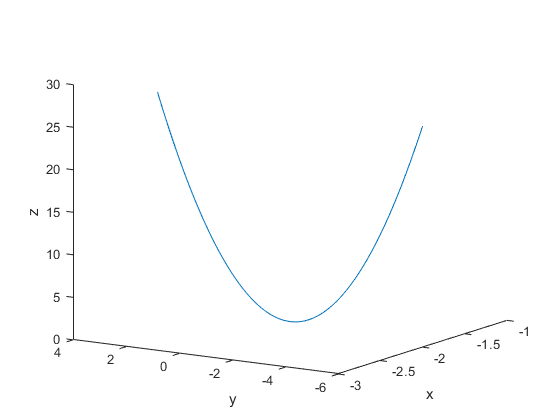
\includegraphics[width=3.5in,height=2.0in]{2_11_7_1.png}
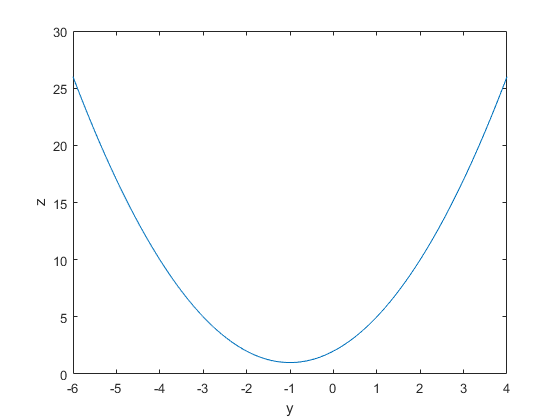
\includegraphics[width=3.5in,height=2.0in]{2_11_7_2.png}
It is easy to see that with increasing $t$, ${\bf r}(t)$ increases in the positive $y$ direction (due to the increasing nature of $t-1$). The position vectors ${\bf r}(0)$, ${\bf r}(1)$, ${\bf r}(2)$ are given by
\begin{eqnarray*}
{\bf r}(0)&=&\la 2,-1,1 \ra\\
{\bf r}(1)&=&\la 2,0,2 \ra\\
{\bf r}(2)&=&\la 2,1,5 \ra
\end{eqnarray*} 
I will sketch these on the plot of ${\bf r}_1(t)$ for simplicity. ${\bf r}(0)$, ${\bf r}(1)$, ${\bf r}(2)$ are in red/orange, yellow, and purple, respectively
\begin{center}
\begin{figure}
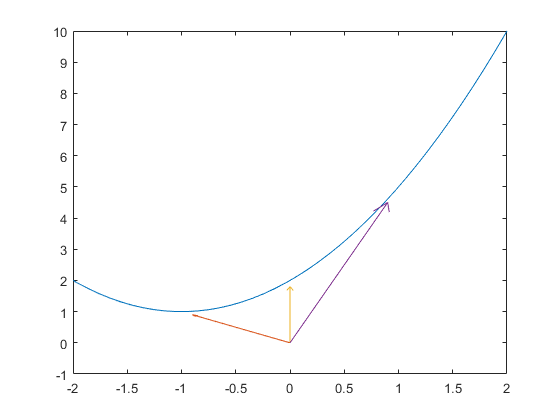
\includegraphics[width=3.5in,height=2.0in]{2_11_7_3.png}
\end{figure}
\end{center}
Next we must find ${\bf r}'(0)$, ${\bf r}'(1)$, ${\bf r}'(2)$. It should be clear that ${\bf r}'(t)=\la 0,1,2t \ra$. Thus we have
\begin{eqnarray*}
{\bf r}'(0)&=&\la 0,1,0 \ra\\
{\bf r}'(1)&=&\la 0,1,2 \ra\\
{\bf r}'(2)&=&\la 0,1,4 \ra
\end{eqnarray*}
Again, these will be sketched on the plot of ${\bf r}_1(t)$. To the left are just the three tangent vectors, to the right are both tangent and position vectors.
\\
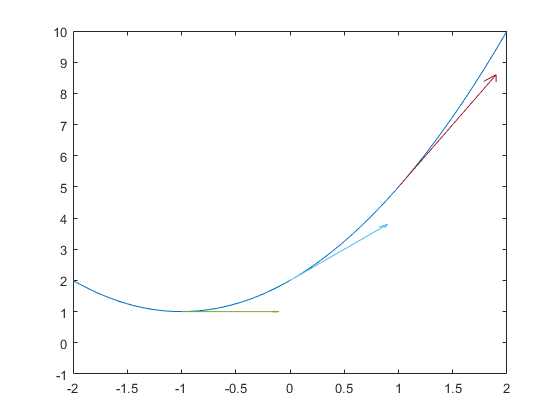
\includegraphics[width=3.5in,height=2.0in]{2_11_7_4.png}
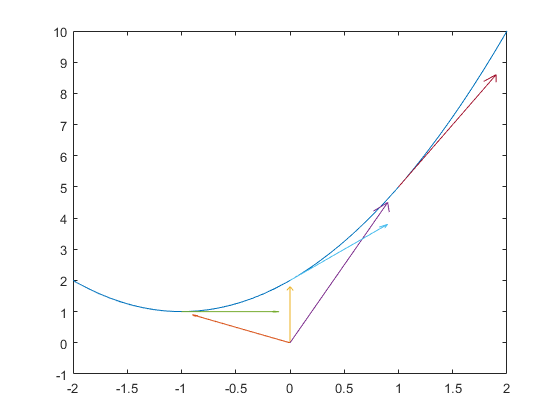
\includegraphics[width=3.5in,height=2.0in]{2_11_7_5.png}
\\
${\bf R}(t)$ simply traces the same curve but in the opposite direction. The final plot is produced below, with $t=0$ corresponding to red/orange, $t=1$ with yellow, and $t=2$ with purple as before (note: ${\bf R}(0)$ and ${\bf R}(1)$ are parallel, so their position vectors overlap).
\begin{center}
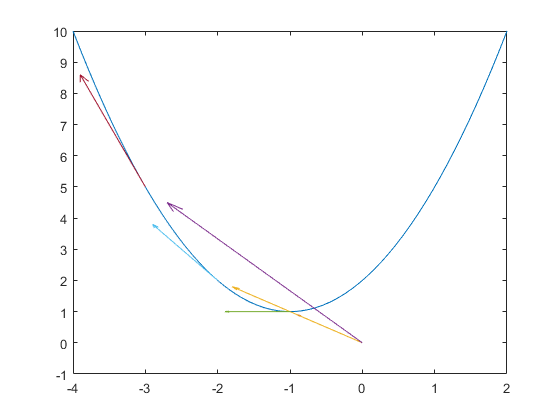
\includegraphics[width=3.5in,height=2.0in]{2_11_7_6.png}
\end{center}
\noindent
{\small {\bf 8}--{\bf 12}}. Determine if the curve traced out by each of the following vector
functions is smooth for a specified interval of the parameter. If the curve is
not smooth at a particular point, graph it near that point.
\begin{enumerate}
  \item[{\small\bf 8}.] ${\bf r}(t)=\la t, \ t^2, \ t^3\ra, \ \ \ 0 \leq t \leq 1$;
  \\
  \\
  {\sc Solution}: A curve is smooth on an interval if its unit tangent vector is continuous on that interval. Recall that the unit tangent vector is given by
  $$\hat{\bf T}(t)=\frac{{\bf r}'(t)}{\|{\bf r}'(t)\|}$$
  so long as ${\bf r}'(t)$ exists and does not vanish. First we find ${\bf r}'(t)$ as
  $${\bf r}'(t)=\la 1,2t,3t^2 \ra$$
  Note that ${\bf r}'(t)$ never vanishes since the first component is always $1$. So $\|{\bf r}'(t)\|$ is
  $$\|{\bf r}'(t)\|=\sqrt{1+4t^2+9t^4}$$
  Then $\hat{\bf T}(t)$ is found to be
  $$\hat{\bf T}(t)=\frac{1}{\sqrt{1+4t^2+9t^4}}\la 1,2t,3t^2 \ra$$
  which is continuous everywhere, hence ${\bf r}'(t)$ is smooth on the interval. 
  \\
  \item[{\small\bf 9}.] ${\bf r}(t)=\la t^2, \ t^3, \ 2 \ra, \ \ \ -1 \leq t \leq 1$;
  \\
  \\
  {\sc Solution}: As above, we must find $\hat{\bf T}$. First we find ${\bf r}'(t)$ as
  $${\bf r}'(t)=\la 2t,3t^2,0 \ra$$
  Note that ${\bf r}'(t)$ vanishes when $t=0$, which is in the given interval. So the unit tangent vector does not exist and ${\bf r}(t)$ is not smooth there. However, we must still determine if the unit tangent vector, when it exists, is continuous. So $\|{\bf r}'(t)\|$ is
  $$\|{\bf r}'(t)\|=\sqrt{4t^2+9t^4}=|t|\sqrt{4+9t^2}$$
  Then $\hat{\bf T}(t)$ is found to be
  $$\hat{\bf T}(t)=\frac{1}{|t|\sqrt{4+9t^2}}\la 2t,3t^2,0 \ra$$
  Note that for $t>0$ we have
  $$\hat{\bf T}(t)=\frac{1}{t\sqrt{4+9t^2}}\la 2t,3t^2,0 \ra=\frac{1}{\sqrt{4+9t^2}}\la 2,3t,0 \ra$$
  which is continuous, and for $t<0$ we have
  $$\hat{\bf T}(t)=\frac{1}{-t\sqrt{4+9t^2}}\la 2t,3t^2,0 \ra=-\frac{1}{\sqrt{4+9t^2}}\la 2,3t,0 \ra$$
  which is also continuous. It becomes evident from this that $\hat{\bf T}(t)$ is discontinuous at $t=0$ as the left and right limits as $t \rightarrow 0$ are not equal. Thus ${\bf r}(t)$ is only not smooth at $t=0$. A sketch is shown below
\begin{center}
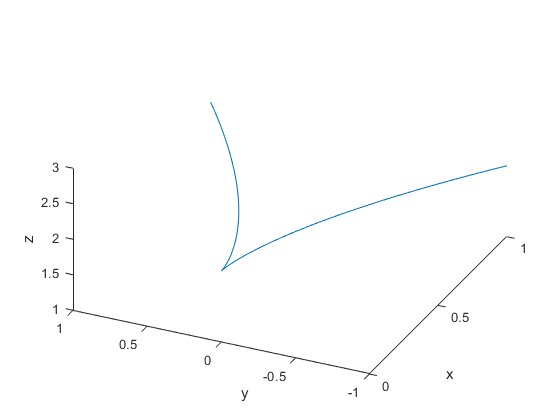
\includegraphics[width=3.5in,height=2.0in]{2_11_9.png}
\end{center}  
  \item[{\small\bf 10}.] ${\bf r}(t)=\la t^{1/3}, \ t, \ t^3\ra, \ \ \ -1 \leq t \leq 1$;
  \\
  \\
  {\sc Solution}: As above, we must find $\hat{\bf T}$. First we find ${\bf r}'(t)$ as
  $${\bf r}'(t)=\la \frac{1}{3}t^{-2/3},1,3t^2 \ra$$
  Note that ${\bf r}'(t)$ never vanishes since the third component is always $1$, but it does not exist when $t=0$ due to the first component. So ${\bf r}(t)$ is possibly not smooth at $t=0$. However, we must still determine if it is not smooth anywhere else in the interval. So $\|{\bf r}'(t)\|$ is
  $$\|{\bf r}'(t)\|=\sqrt{\frac{1}{9}t^{-4/3}+1+9t^4}$$
  Then $\hat{\bf T}(t)$ is found to be
\begin{eqnarray*}
\hat{\bf T}(t)&=&\frac{1}{\sqrt{\frac{1}{9}t^{-4/3}+1+9t^4}}\la \frac{1}{3}t^{-2/3},1,3t^2 \ra=\frac{3t^{2/3}}{\sqrt{1+9t^{4/3}+81t^{16/3}}}\la \frac{1}{3}t^{-2/3},1,3t^2 \ra\\
&=&\frac{1}{\sqrt{1+9t^{4/3}+81t^{16/3}}}\la 1,3t^{2/3},9t^{8/3} \ra
\end{eqnarray*}  
It ends up being that $\hat{\bf T}(t)$ is not smooth at $t=0$, illustrated below
\begin{center}
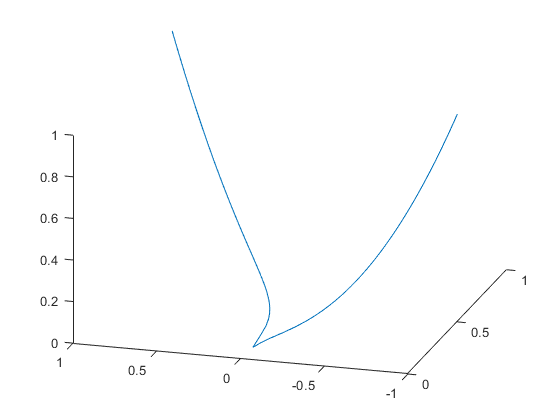
\includegraphics[width=3.5in,height=2.0in]{2_11_10.png}
\end{center} 
  \item[{\small\bf 11}.] ${\bf r}(t)=\la t^5, \ t^3, \ t^4\ra, \ \ \ -1 \leq t \leq 1$;
  \\
  \\
  {\sc Solution}: As above, we must find $\hat{\bf T}$. First we find ${\bf r}'(t)$ as
  $${\bf r}'(t)=\la 5t^4,3t^2,4t^3 \ra$$
  Note that ${\bf r}'(t)$ exists everywhere but vanishes at $t=0$. So ${\bf r}(t)$ is possibly not smooth at $t=0$. However, we must still determine if it is not smooth anywhere else in the interval. So $\|{\bf r}'(t)\|$ is
  $$\|{\bf r}'(t)\|=\sqrt{25t^8+9t^4+16t^6}=|t^2|\sqrt{25t^4+9+16t^2}=t^2\sqrt{9+16t^2+25t^4}$$
  Then $\hat{\bf T}(t)$ is found to be
$$\hat{\bf T}(t)=\frac{1}{t^2\sqrt{9+16t^2+25t^4}}\la 5t^4,3t^2,4t^3 \ra=\frac{1}{\sqrt{9+16t^2+25t^4}}\la 5t^2,3,4t \ra$$
It ends up being that $\lim_{t \rightarrow 0}\hat{\bf T}(t)$ exists and is $\la 0,1,0\ra$. So ${\bf r}(t)$ is smooth everywhere in the interval.
\\
  \item[{\small\bf 12}.] ${\bf r}(t)=\la \sin^3 t, \ 1, \ t^2 \ra, \ \ \ -\pi/2 \leq t \leq \pi/2$.
  \\
  \\
  {\sc Solution}: As above, we must find $\hat{\bf T}$. First we find ${\bf r}'(t)$ as
  $${\bf r}'(t)=\la 3\sin^2t\cos t, 0, 2t \ra$$
  Note that ${\bf r}'(t)$ exists everywhere but vanishes at $t=0$. So ${\bf r}(t)$ is possibly not smooth at $t=0$. However, we must still determine if it is not smooth anywhere else in the interval. So $\|{\bf r}'(t)\|$ is
  $$\|{\bf r}'(t)\|=\sqrt{9\sin^4t\cos^2t+4t^2}$$
  Then $\hat{\bf T}(t)$ is found to be
$$\hat{\bf T}(t)=\frac{1}{\sqrt{9\sin^4t \cos^2t+4t^2}}\la 3\sin^2t\cos t, 0, 2t \ra$$
Note that 
$$\lim_{t \rightarrow 0+}T_3(t)=\lim_{t \rightarrow 0+}\frac{2t}{\sqrt{9\sin^4 t \cos^2 t+4t^2}}=1$$
whereas
$$\lim_{t \rightarrow 0-}T_3(t)=\lim_{t \rightarrow 0-}\frac{2t}{\sqrt{9\sin^4 t \cos^2 t+4t^2}}=-1$$
and thus the limit does not exist, so ${\bf r}(t)$ is not smooth at $t=0$. The curve is shown below
\begin{center}
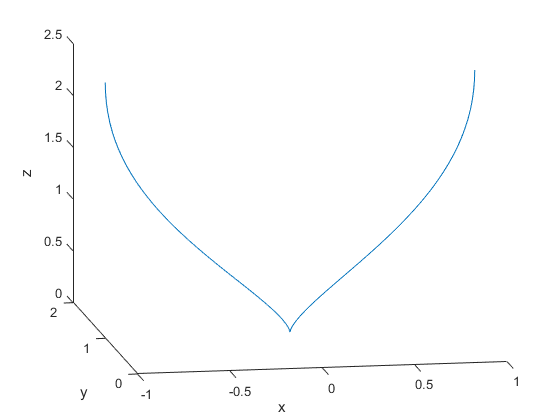
\includegraphics[width=3.5in,height=2.0in]{2_11_12.png}
\end{center} 
\end{enumerate}
{\small\bf 13}. Determine whether a cardioid described by the polar graph $r = 1 -
a \cos \theta$, $0 \leq \theta \leq 2\pi$, is smooth, where $|a| \leq 1$. Sketch the cardioid for $a = 0$,
$a = \pm1/2$, and $a = \pm1$. Hint: to find parametric equations of the cardioid,
use the relations between the polar and rectangular coordinates and $\theta$ as a
parameter.
\\
\\
{\sc Solution}: First I will write $t$ instead of $\theta$; this is purely a cosmetic change. Recall that the conversion from polar to rectangular coordinates is $x(t)=r\cos t$, $y(t)=r\sin t$. So ${\bf r}(t)=\la (1-a\cos t)\cos t, (1-a\cos t)\sin t\ra$ describes the cardioid. From this we must find the unit tangent vector. We have that
\begin{eqnarray*}
{\bf r}'(t)&=&\la -(1-a\cos t)\sin t+(a\sin t)\cos   t, (1-a\cos t)\cos t+(a\sin t)\sin t \ra \\
&=& \la -\sin t+2a\sin t\cos t, \cos t-a\cos^2 t+a\sin^2 t \ra\\
&=&\la -\sin t+a\sin (2t), \cos t-a\cos(2t) \ra\\
\|{\bf r}'(t)\|&=&\sqrt{(-\sin t+a\sin (2t))^2+(\cos t-a\cos(2t))^2}\\
&=&\sqrt{\sin^2 t -2a\sin t\sin(2t) +a^2\sin^2 (2t)+\cos^2 t -2a\cos t\cos(2t) +a^2\cos^2 (2t)}\\
&=&\sqrt{(\sin^2 t+\cos^2 t)+(a^2\sin^2 (2t)+a^2\cos^2 (2t))-2a(\sin t\sin(2t)+\cos t\cos(2t))}\\
&=&\sqrt{1+a^2-2a\cos t}
\end{eqnarray*}
It follows then that ${\bf r}(t)$ never vanishes so long as $(-2\cos t)^2-4 <0 \ \Leftrightarrow \ 4\cos^2 t <4$. This inequality is broken $t=0, \pi, 2\pi$. However, when $t=\pi$, $1+a^2-2a\cos t= 1+a^2+2a=(1+a)^2$, which is nonnegative so long as $a\neq -1$. When $t=0, 2\pi$, $1+a^2-2a\cos t= 1+a^2-2a=(1-a)^2$, which is nonnegative so long as $a\neq 1$. For any other combination of $a,t$, $\|{\bf r}'(t)\|$ is nonzero. Then the unit tangent vector can be defined as
$$\hat{\bf T}(t)=\frac{1}{\sqrt{1+a^2-2a\cos t}}\la (1-a\cos t)\cos t, (1-a\cos t)\sin t\ra$$
Again, when $a=-1$, ${\bf r}(t)$ is not smooth at $t=\pi$ and when $a=1$, ${\bf r})(t)$ is not smooth at $t=0, 2\pi$. The graphs are depicted below:
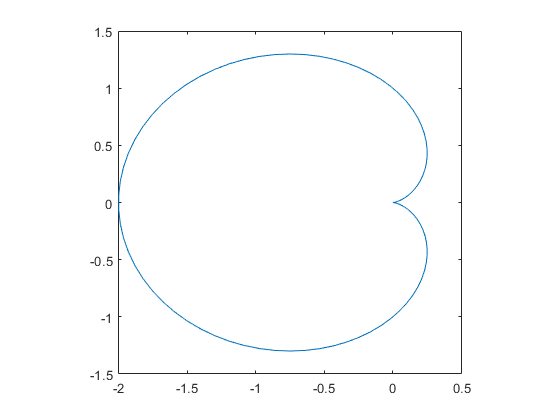
\includegraphics[width=3.5in,height=2.0in]{2_11_13_1.png}
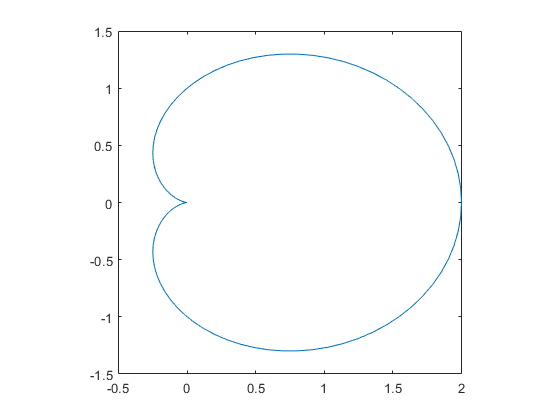
\includegraphics[width=3.5in,height=2.0in]{2_11_13_5.png}
\begin{center}
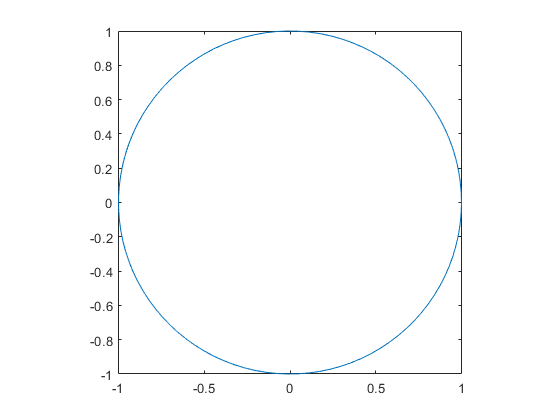
\includegraphics[width=3.5in,height=2.0in]{2_11_13_3.png}
\end{center}
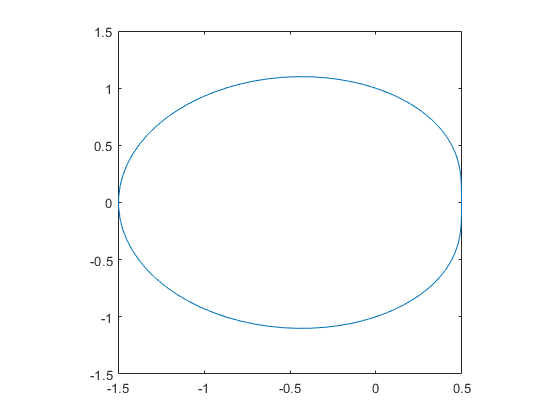
\includegraphics[width=3.5in,height=2.0in]{2_11_13_2.png}
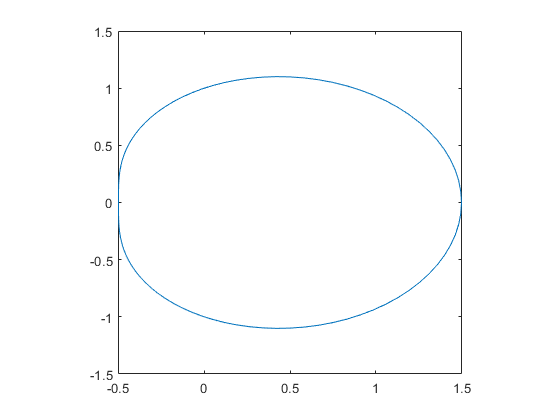
\includegraphics[width=3.5in,height=2.0in]{2_11_13_4.png}
From left to right, top to bottom: $a=1,-1,0,1/2,-1/2$.
\\
\\
\noindent
{\small {\bf 14}--{\bf 15}}. Find the parametric equations of the tangent line to each of the
following curves at a specified point:
\begin{enumerate}
  \item[{\small\bf 14}.] ${\bf r}(t)=\la t^2-t,\ t^3/3,\ 2t\ra, \ P_0=(6,9,6)$;
  \\
  \\
  {\sc Solution}: We begin by finding the value of $t$ such that ${\bf r}(t)=\overrightarrow{OP_0}$. Thus we have $t^3/3=9 \ \Leftrightarrow \ t^3=27 \ \Leftrightarrow \ t=3$. Next we find ${\bf r}'(t)$ by differentiating each component,
  $${\bf r}'(t)=\la 2t-1,t^2,2 \ra$$
  Then ${\bf r}'(3)=\la 5,9,2 \ra$, which is parallel to the tangent line at $P_0$. Recall that in general a line parallel to a vector ${\bf v}=\la v_i, v_j, v_k\ra$ passing through a $P_0=(x_0,y_0,z_0)$ is given by
  $${\bf R}(t)=\overrightarrow{OP_0}+t{\bf v},$$
  with parametric equations given by $x=x_0+tv_i$, $y=y_0+tv_j$, and $z=z_0+tv_k$. Thus the parametric equations of the tangent line are
  $$x=6+5t, \ \ y=9+9t, \ \ z=6+2t$$
  \item[{\small\bf 15}.] ${\bf r}(t)=\la \ln t,\ 2\sqrt{t},\ t^2\ra, \ P_0=(0,2,1)$.
  \\
  \\
  {\sc Solution}: As above, we begin by finding the value of $t$ such that ${\bf r}(t)=\overrightarrow{OP_0}$. Thus we have $2\sqrt{t}=2 \ \Leftrightarrow \ =1$. Next we find ${\bf r}'(t)$.
  $${\bf r}'(t)=\la 1/t, 1/\sqrt{t}, 2t\ra$$
  Then ${\bf r}'(1)=\la 1,1,2 \ra$. So the parametric equations of a line tangent to $P_0$ are
  $$x=t, \ \ y=2+t, \ \ z=1+2t$$
\end{enumerate}
\noindent
{\small {\bf 16}--{\bf 17}}. Find the unit tangent vector to the curve traversed by the specified
vector function at the given point $P_0$:
\begin{enumerate}
  \item[{\small\bf 16}.] ${\bf r}(t)=\la 2t+1,\ 2\arctan t,\ e^{-t}\ra, \ P_0=(1,0,1)$;
  \\
  \\
  {\sc Solution}: First we find the value of $t$ such that ${\bf r}(t)=\overrightarrow{OP_0}$. Then $e^{-t}=1 \ \Leftrightarrow  \ t=0$. Next we find ${\bf r}'(t)$ by differentiating each component as follows:
  $${\bf r}'(t)=\la 2,2/(1+t^2),-e^{-t} \ra$$
  Then ${\bf r}'(0)=\la 2,2,-1 \ra$. So $\|{\bf r}'(0)\|=\sqrt{2^2+2^2+1}=\sqrt{9}=3$
  So the unit tangent vector is
  $$\hat{\bf T}(0)=\frac{{\bf r}'(0)}{\|{\bf r}'(0)\|}=\frac{1}{3}\la 2,2,-1 \ra$$
  \item[{\small\bf 17}.] ${\bf r}(t)=\la \cos(\omega t),\ \cos(3\omega t),\ \sin(\omega t)\ra, \ P_0=(1/2,-1,\sqrt{3}/2)$, where $\omega$ is a positive constant.
  \\
  \\
  {\sc Solution}: As above we find the value of $t$ such that ${\bf r}(t)=\overrightarrow{OP_0}$. Then $\cos(\omega t)=1/2$, so $t=\pi/(3\omega)$ or $t=5\pi/(3\omega)$. Of these, only $t=\pi/(3\omega)$  satisfies $\sin(\omega t)=\sqrt{3}/2$. Of course, adding multiples of $2\pi/\omega$ to $t$ will also produce valid $t$, but these may be neglected; the effect is to essentially add $0$. Next we find ${\bf r}'(t)$ by differentiating each component as follows:
  $${\bf r}'(t)=\la -\omega\sin(\omega t),-3\omega\sin(3\omega t),\omega\cos(\omega t) \ra$$
  Then ${\bf r}'(\pi/(3\omega))=\la -\omega \sqrt{3}/2,0,\omega/2 \ra$. So $\|{\bf r}'(\pi/(3\omega))\|=\sqrt{\omega^2(3/4)+0+\omega^2/4}=\omega$
  So the unit tangent vector is
  $$\hat{\bf T}(\pi/(3\omega))=\frac{{\bf r}'(\pi/(3\omega))}{\|{\bf r}'(\pi/(3\omega))\|}=\frac{1}{\omega}\la -\omega \sqrt{3}/2,0,\omega/2 \ra=\la -\sqrt{3}/2,0,1/2 \ra$$
\end{enumerate}
{\small\bf 18}. Find ${\bf r}'(t)\cdot{\bf r}''(t)$ and ${\bf r}'(t)\times{\bf r}''(t)$ if ${\bf r}(t)=\la t, \ t^2-1, \ t^3+2\ra$.
\\
\\
{\sc Solution}: First we compute ${\bf r}'(t)$ and ${\bf r}''(t)$ as follows:
\begin{eqnarray*}
{\bf r}'(t)&=&\la 1,2t,3t^2 \ra\\
{\bf r}''(t)&=&\la 0,2, 6t \ra
\end{eqnarray*}
Then ${\bf r}'(t)\cdot {\bf r}''(t)$ is
$${\bf r}'(t)\cdot {\bf r}''(t)=\la 1,2t,3t^2 \ra\cdot \la 0,2,6t \ra = 4t+18t^3 $$
And ${\bf r}'(t)\times {\bf r}''(t)$ is 
$${\bf r}'(t)\times {\bf r}''(t)=\det
\begin{pmatrix}
\hat{\bf e}_1 & \hat{\bf e}_2 & \hat{\bf e}_3\cr 1&2t&3t^2\cr 0&2&6t \end{pmatrix}=\la \det\begin{pmatrix}2t&3t^2\cr 2&6t  \end{pmatrix}, -\det\begin{pmatrix}1&3t^2\cr 0&6t  \end{pmatrix}, \det\begin{pmatrix}1&2t\cr 0&2 \end{pmatrix} \ra = \la 6t^2, -6t, 2 \ra$$
\\
{\small\bf 19}. Is there a point on the curve ${\bf r}(t)=\la t^2-t, \ t^3/3, \ 2t \ra$ at which the
tangent line is parallel to the vector ${\bf v} = \la-5/2, 2, 1\ra$? If so, find the point.
\\
\\
{\sc Solution}: We must first compute ${\bf r}'(t)$ as follows
$${\bf r}'(t)=\la 2t-1, t^2, 2\ra$$
If there is a point on the curve ${\bf r})(t)$ such that the tangent line is parallel to ${\bf v}$, then there must exist an $s$ and $t$ such that ${\bf v}=s{\bf r}'(t)$. So we have
$$\la -5/2,2,1\ra = \la 2ts-s, t^2s, 2s \ra$$
Equating the third components yields $2s = 1 \ \Leftrightarrow \ s=1/2$. Equating the second components and substituting $s=1/2$ yields $2=t^2/2 \ \Leftrightarrow \ t=\pm 2$. With $t=-2$ we have $2(-2)/2-1/2=-5/2$ and with $t=2$ we have $2(2)/2-1/2=3/2$. Thus there is a point, when $t=-2$, ${\bf r}(-2)=\la 2, -8/3, -4\ra$.  
\\
\\
{\small\bf 20}. Let ${\bf r}(t)=\la e^t, 2\cos t, \sin(2t) \ra$. Use the best linear approximation
${\bf L}(t)$ near $t = 0$ to estimate ${\bf r}(0.2)$. Use a calculator to assess the accuracy
$\|{\bf r}(0.2)-{\bf L}(0.2)\|$ of the estimate. Repeat the procedure for ${\bf r}(0.7)$ and ${\bf r}(1.2)$. Compare the errors in all three cases.
\\
\\
{\sc Solution}: Recall that the best linear approximation, ${\bf L}(t)$, near a point $t=t_0$ is defined to be
$${\bf L}(t)={\bf r}(t_0)+(t-t_0){\bf r}'(t_0)$$
So we must first calculate ${\bf r}'(t)$, which is
$${\bf r}'(t)=\la e^t, -2\sin t, 2\cos(2t)\ra$$
Then we have that ${\bf r}(0)=\la 1,2,0 \ra$ and ${\bf r}'(0)=\la 1,0,2\ra$. So then ${\bf L}(t)$ around $t=0$ is
$${\bf L}(t)=\la 1,2,0 \ra + t\la 1,0,2\ra= \la 1+t, 2, 2t \ra.$$
We have that ${\bf r}(0.2)\approx{\bf L}(0.2)$, so
$${\bf r}(0.2)\approx{\bf L}(0.2)=\la 1.2, 2,0.4 \ra$$
Using a calculator to compute $\|{\bf r}(0.2)-{\bf L}(0.2)\|$ gives
$$\|{\bf r}(0.2)-{\bf L}(0.2)\|=0.0464695041096$$
For $t=0.7$ and $t=1.2$ we have
$${\bf r}(0.7)\approx{\bf L}(0.7)=\la 1.7, 2,1.4 \ra, \ \ \ {\bf r}(1.2)\approx{\bf L}(1.2)=\la 2.2, 2,2.4 \ra$$
And so
$$\|{\bf r}(0.7)-{\bf L}(0.7)\|=0.701063103676, \ \ \ \|{\bf r}(1.2)-{\bf L}(1.2)\|=2.419718929$$
Clearly the error increases as $t$ moves away from $0$. This makes sense as the approximation is accurate for small neighborhoods of $t_0$. 
\\
\\
{\small\bf 21}. Find the point of intersection of the plane $y + z = 3$ and the curve ${\bf r}(t)=\la \ln t, \ t^2, \ 2t \ra$. Find the angle between the normal of the plane and the tangent line to the curve at the point of intersection.
\\
\\
{\sc Solution}: To find the point of intersection simply substitute $y(t)$, $z(t)$ into the equation of the plane and solve for $t$:
$$t^2+2t=3 \ \Leftrightarrow \ t^2+2t-3=0 \ \Leftrightarrow \ (t+3)(t-1)=0 \ \Leftrightarrow \ t=-3,1$$
Since $\ln(-3)$ is not real, the only point of intersection is when $t=1$, at ${\bf r}(1)=\la 0,1,2 \ra$. The normal of the plane is ${\bf n}=\la 0,1,1 \ra$. The tangent line to the curve at the point of intersection is parallel to ${\bf r}'(1)$. First we must compute ${\bf r}'(t)$, which is
$${\bf r}'(t)=\la 1/t, 2t, 2 \ra$$
Then ${\bf r}'(1)=\la 1,2,2 \ra$. So the angle between the tangent line and the normal of the plane is simply the angle between ${\bf r}'(1)$ and ${\bf n}$, which is
$$\theta=\arccos(\frac{{\bf r}'(1)\cdot{\bf n}}{\|{\bf r}'(1)\|\|{\bf n}\|})=\arccos(\frac{2+2}{\sqrt{1+4+4}\sqrt{1+1}})=\arccos(\frac{4}{3\sqrt{2}})$$
\\
{\small\bf 22}. Does the curve ${\bf r}(t)=\la 2t^2, \ 2t, \ 2-t^2 \ra$ intersect the plane $x+y+z = -3$?
If not, find a point on the curve that is closest to the plane. What is the
distance between the curve and the plane. Hint: Express the distance between
a point on the curve and the plane as a function of $t$, then solve the extreme value problem.
\\
\\
{\sc Solution}: To test if ${\bf r}(t)$ intersects the plane, substitute $x(t)$, $y(t)$, and $z(t)$ into the equation of the plane and attempt to solve for $t$ as follows:
$$2t^2+2t+2-t^2=-3 \ \Leftrightarrow \ t^2+2t+3=0$$
The discriminant of this quadratic (in $t$) is $4-4(3)(1)<0$, so there are no real solutions. Thus there is no point of intersection. 
\\
Recall that the distance between a point, whose position vector is ${\bf r}_1$, and a plane is
$$D=\frac{|{\bf n}\cdot{\bf r}_1-d|}{\|{\bf n}\|}$$
Here we are interested in the closest distance between the curve and the plane, so we let ${\bf r}_1={\bf r}(t)$, and $D$ becomes a function of $t$. We may then minimize $D$ by computing its derivative and finding the critical points as follows
$$D'(t)=(\frac{|{\bf n}\cdot{\bf r}(t)-d|}{\|{\bf n}\|})'=\frac{|({\bf n})'\cdot({\bf r}(t)-{\bf r}_0))+({\bf n})\cdot({\bf r}(t)-{\bf r}_0))'|}{\|{\bf n}\|}=\frac{|{\bf n}\cdot{\bf r}'(t)|}{\|{\bf n}\|}$$
$D$ has a critical value when  ${\bf n}\cdot{\bf r}'(t)=0$. We first compute ${\bf r}'(t)$ as 
$${\bf r}'(t)=\la 4t,2,-2t \ra$$
Then to satisfy the condition ${\bf n}\cdot{\bf r}'(t)=0$ we must have
$$4t+2-2t=0 \ \Leftrightarrow \ t=-1$$
So ${\bf n}\cdot{\bf r}(t)=2t^2+2t+2-t^2=t^2+2t+2=(t+1)^2+1$. Thus ${\bf n}\cdot{\bf r}(-1)=1$. It follows that the minimum distance is
$$D(-1)=\frac{|1-(-3)|}{\sqrt{1+1+1}}=\frac{4}{\sqrt{3}}$$
An alternative solution can be found below.
\\
\\
Recall that the distance between a point $P$ on a curve and a plane is the distance of $QP$, where $QP$ is orthogonal to the plane and $Q$ is on the plane. The question can now be reformulated as to minimize the distance $QP$. We want $\overrightarrow{QP}$ to be parallel to ${\bf n}=\la 1,1,1\ra$, so $\la 2t^2-x_0, 2t-y_0, 2-t^2-z_0\ra=s\la 1,1,1 \ra$ for some $s$, where $(x_0,y_0,z_0)$ is a point on the plane. Then $z_0=-3-x_0-y_0$. Furthermore, $2t-y_0=s$, so $2t^2-x_0=s=2t-y_0 \ \Leftrightarrow \ 2t^2-2t-x_0+y_0=0$. Finally $2-t^2+3+x_0+y_0=2t^2-x_0 \ \Leftrightarrow \ 5-3t^2+2x_0+y_0=0$. Adding two times the first to the second gives $t^2-4t+5+3y_0=0 \ \Leftrightarrow \ y_0=-1/3(t^2-4t+5)$. Solving for $s$ gives $s=2t-y_0=2t+1/3(t^2-4t+5)=t^2/3+2/3t+5/3$. Note then that $|QP|=\|\overrightarrow{QP}\|=\|s\la 1,1,1 \ra\|$, and so we need only minimize $s$. We have that
$$s=1/3(t^2+2t+5)$$
and so 
$$s'(t)=1/3(2t+2)$$
and $s$ attains a minimum when $t=-1$. The minimum value of $s$ then is $s=1/3(1-2+5)=4/3$. Finally, the minimum distance is
$$|QP|=|s|\|\la 1,1,1 \ra \|=4/3\sqrt{3}=4/\sqrt{3}$$
{\small\bf 23}. Find the point of intersection of two curves ${\bf r}_1(t)=\la t, \ 1-t, \ 3+t^2 \ra$ and ${\bf r}_2(s)=\la 3-s, \ s-2, \ s^2 \ra$. If the angle at which two curves intersect is defined
as the angle between their tangent lines at the point of intersection, find the
angle at which the above two curves intersect.
\\
\\
{\sc Solution}: To find a point of intersection we must find an $s,t$ such that ${\bf r}_1(t)={\bf r}_2(s)$. So we have
$$\la t,1-t, 3+t^2 \ra = \la 3-s, s-2, s^2 \ra$$
Equating the first components gives $t=3-s$. Equating the third components and substituting this gives $3+9-6s+s^2=s^2 \ \Leftrightarrow \ s=2$. Thus $t=1$. It is easily verified that ${\bf r}_1(1)=\la 1,0,4 \ra$ and ${\bf r}_2(2)=\la 1,0,4 \ra$, which are indeed equal. The angle between the tangent lines is equal to the angle between the vectors parallel to the tangent lines, of which we may choose ${\bf r}_1'(1)$ and ${\bf r}_2'(2)$. We have that
\begin{eqnarray*}
{\bf r}_1'(t)&=&\la 1,-1, 2t \ra\\
{\bf r}_2'(s)&=&\la -1,1,2s \ra
\end{eqnarray*}
So ${\bf r}_1'(1)=\la 1,-1,2 \ra$ and ${\bf r}_2'(2)=\la -1,1,4 \ra$. Therefore the angle is
$$\theta=\arccos(\frac{{\bf r}_1'(1)\cdot{\bf r}_2'(2)}{\|{\bf r}_1'(1)\|\|{\bf r}_2'(2)\|})=\arccos(\frac{-1-1+8}{\sqrt{1+1+4}\sqrt{1+1+16}})=\arccos(\frac{6}{\sqrt{6}\sqrt{18}})=\arccos(\frac{1}{\sqrt{3}})$$
{\small\bf 24}. State the condition under which the tangent lines to the curve ${\bf r}(t)$
at two distinct points ${\bf r}(t_1)$ and ${\bf r}(t_2)$ are intersecting, or skew, or parallel.
Let ${\bf r}(t)=\la 2\sin(\pi t), \ \cos(\pi t), \ \sin(\pi t) \ra$, $t_1 = 0$, and $t_2 = 1/2$. Determine whether the tangent lines at these points are intersecting and, if so, find the
point of intersection.
\\
\\
{\sc Solution}: Recall the conditions for which two lines are intersecting, skew, or parallel:
\\
Let $\mathcal{L}_1$ be a line through $P_1$ and parallel to ${\bf v}_1$ and $\mathcal{L}_2$ a line through $P_2$ parallel to ${\bf v}_2$. Set ${\bf r}_{12}=\overrightarrow{P_1P_2}$ Then
\\
1. $\mathcal{L}_1$ and $\mathcal{L}_2$ are intersecting iff
$${\bf r}_{12}\cdot({\bf v}_1\times{\bf v}_2)= 0, \ \ {\bf v}_1\times{\bf v}_2 \neq {\bf 0}$$
2. $\mathcal{L}_1$ and $\mathcal{L}_2$ are skew iff
$${\bf r}_{12}\cdot({\bf v}_1\times{\bf v}_2)\neq 0$$
3. $\mathcal{L}_1$ and $\mathcal{L}_2$ are parallel iff
$${\bf v}_1\times{\bf v}_2={\bf 0}, \ {\bf r}_{12}\times{\bf v}_1 \neq {\bf 0}$$
Simply let ${\bf v}_1={\bf r}'(t_1)$, ${\bf v}_1={\bf r}'(t_2)$, and ${\bf r}_{12}={\bf r}(t_2)-{\bf r}(t_1)$ (the order does not matter) to formulate the condition under which the tangent lines are intersecting, skew, or parallel.
\\
With ${\bf r}(t)=\la 2\sin(\pi t), \ \cos(\pi t), \ \sin(\pi t) \ra$, $t_1 = 0$, and $t_2 = 1/2$, first find ${\bf r}'(t_1)$ and ${\bf r}'(t_2)$ as follows:
$${\bf r}'(t)=\la 2\pi\cos(\pi t), -\pi \sin(\pi t), \pi \cos(\pi t) \ra$$
Then ${\bf r}'(0)=\la 2\pi ,0 ,\pi \ra$ and ${\bf r}'(1/2)=\la 0, -\pi , 0 \ra$. The cross product ${\bf r}'(0)\times{\bf r}'(1/2)$ can easily be found to be $\la \pi^2, 0, -2\pi^2 \ra \neq {\bf 0}$. So the lines are either intersecting or skew, and we must calculate ${\bf r}(1/2)-{\bf r}(0)$ to determine which. Evidently ${\bf r}(1/2)=\la 2,0,1 \ra$ and ${\bf r}(0)=\la 0,1,0 \ra$, so ${\bf r}(1/2)-{\bf r}(0)=\la 2,-1,1 \ra$. The triple product $({\bf r}(1/2)-{\bf r}(0))\cdot({\bf r}'(0)\times{\bf r}'(1/2))$ can then be calculated as 
$$({\bf r}(1/2)-{\bf r}(0))\cdot({\bf r}'(0)\times{\bf r}'(1/2)) = \la 2,-1,1 \ra \cdot \la \pi^2,0,-2\pi^2 \ra =2\pi^2-2\pi^2= 0$$
Therefore the lines are skew.
\\
\\
{\small\bf 25}. Suppose a smooth curve ${\bf r}(t)$ does not intersect a plane through a point
$P_0$ and orthogonal to a vector ${\bf n}$. Assume that, among the points on the curve, there is one that is closest to the plane. What is the angle between ${\bf n}$ and a tangent vector to the curve at the point that is the closest to the plane?
\\
\\
{\sc Solution}: Let ${\bf r}_0$ be the position vector for $P_0$. Recall that the distance between a point, whose position vector is ${\bf r}_1$, and a plane is
$$D=\frac{|{\bf n}\cdot({\bf r}_1-{\bf r}_0)|}{\|{\bf n}\|}$$
Here we are interested in the closest distance between the curve and the plane, so we let ${\bf r}_1={\bf r}(t)$, and $D$ becomes a function of $t$. We may then minimize $D$ by computing its derivative and finding the critical points as follows
$$D'(t)=(\frac{|{\bf n}\cdot({\bf r}(t)-{\bf r}_0)|}{\|{\bf n}\|})'=\frac{|({\bf n})'\cdot({\bf r}(t)-{\bf r}_0))+({\bf n})\cdot({\bf r}(t)-{\bf r}_0))'|}{\|{\bf n}\|}=\frac{|{\bf n}\cdot{\bf r}'(t)|}{\|{\bf n}\|}$$
$D$ has a critical value when  ${\bf n}\cdot{\bf r}'(t)=0$, i.e. when ${\bf n}$ and ${\bf r}'(t)$ are orthogonal, so the angle is $\pi/2$.
\\
\\
{\small\bf 26}. Suppose ${\bf r}(t)$ is twice differentiable. Show that $({\bf r}(t)\times{\bf r}'(t))'={\bf r}(t)\times {\bf r}''(t)$.
\\
\\
{\sc Solution}: First recall the differentiation rule for cross products:
$$({\bf v}(t)\times{\bf u}(t))'={\bf v}'(t)\times{\bf u}(t)+{\bf v}(t)\times{\bf u}'(t)$$
The proof follows easily:
$$({\bf r}(t)\times{\bf r}'(t))'=({\bf r}(t))'\times({\bf r}'(t))+({\bf r}(t))\times({\bf r}'(t))'={\bf r}'(t)\times{\bf r}'(t)+{\bf r}(t)\times{\bf r}''(t)={\bf r}(t)\times {\bf r}''(t)$$
owing to the fact that ${\bf v}\times{\bf v}={\bf 0}$ for any vector $\bf v$.
\\
\\
{\small\bf 27}. Suppose that ${\bf r}(t)$ is differentiable three times. Show that $[{\bf r}(t)\cdot({\bf r}'(t)\times{\bf r}''(t))]'={\bf r}(t)\cdot({\bf r}'(t)\times{\bf r}'''(t))$. 
\\
\\
{\sc Solution}: Recall the differentiation rule for dot products:
$$({\bf v}(t)\cdot{\bf u}(t))'={\bf v}'(t)\cdot{\bf u}(t)+{\bf v}(t)\cdot{\bf u}'(t)$$
Then we have
\begin{eqnarray*}
[{\bf r}(t)\cdot({\bf r}'(t)\times{\bf r}''(t))]'&=&
({\bf r}(t))'\cdot({\bf r}'(t)\times{\bf r}''(t))+({\bf r}(t))\cdot({\bf r}'(t)\times{\bf r}''(t))'
\\
&=&{\bf r}'(t)\cdot({\bf r}'(t)\times{\bf r}''(t))+{\bf r}(t)\cdot({\bf r}'(t)\times{\bf r}''(t))'={\bf r}(t)\cdot({\bf r}'(t)\times{\bf r}''(t))'
\end{eqnarray*}
owing to the fact that ${\bf v}\cdot ({\bf v}\times{\bf u})=0$ for vectors ${\bf v}, {\bf u}$. 
Next recall the differentiation rule for cross products:
$$({\bf v}(t)\times{\bf u}(t))'={\bf v}'(t)\times{\bf u}(t)+{\bf v}(t)\times{\bf u}'(t)$$
The proof now follows:
\begin{eqnarray*}
{\bf r}(t)\cdot({\bf r}'(t)\times{\bf r}''(t))'&=&{\bf r}(t)\cdot[({\bf r}'(t))'\times({\bf r}''(t))+({\bf r}'(t))\times({\bf r}''(t))']={\bf r}(t)\cdot[{\bf r}''(t)\times{\bf r}''(t)+{\bf r}'(t)\times{\bf r}'''(t)]\\
&=&{\bf r}(t)\cdot({\bf r}'(t)\times{\bf r}'''(t))
\end{eqnarray*}
owing to the fact that ${\bf v}\times{\bf v}={\bf 0}$ for any vector $\bf v$.
\\
\\
{\small\bf 28}. Let ${\bf r}(t)$ be a differentiable vector function. Show that $(\|{\bf r}(t)\|)'={\bf r}(t)\cdot{\bf r}'(t)/\|{\bf r}(t)\|$.
\\
\\
{\sc Solution}: Recall that $\|{\bf r}(t)\|^2={\bf r}(t)\cdot{\bf r}(t) \ \Leftrightarrow \ \|{\bf r}(t)\|=\sqrt{{\bf r}(t)\cdot{\bf r}(t)}$. Using the differentiation rule for dot products we obtain:
$$(\|{\bf r}(t)\|)'=\frac{{\bf r}'(t){\bf r}(t)+{\bf r}(t){\bf r}'(t)}{2\sqrt{{\bf r}(t)\cdot{\bf r}(t)}}=\frac{{\bf r}(t)\cdot{\bf r}'(t)}{\|{\bf r}(t)\|}$$
Clearly this is only defined when $\|{\bf r}(t)\| \neq 0$. 
\\
\\
{\small\bf 29}. A space warship can fire a laser cannon forward along the tangent
line to its trajectory. If the trajectory is traversed by the vector function
${\bf r}(t)=\la t,t,t^2+4\ra$ in the direction of increasing $t$ and the target is the sphere $x^2+y^2+z^2=1$ find the part of the trajectory in which the laser cannon can hit the target. Hint: If a line $\mathcal{L}$ is tangent to the trajectory at $t=t_0$, then the target is hit when the distance between $\mathcal{L}$ and the origin is less or
equal $1$. State this geometrical condition as an algebraic condition on $t_0$. To solve this algebraic condition, show that the trajectory is a parabola in the plane $y = x$. So, find points on the parabola at which its tangent is at
a distance less or equal $1$ to the origin.
\\
\\
{\sc Solution}: A tangent line to the trajectory at $t=t_0$ is given by
$${\bf r}_1(t)={\bf r}(t_0)+(t-t_0){\bf r}'(t_0)=\la t_0, t_0, t_0^2+4 \ra +(t-t_0)\la 1,1, 2t_0 \ra = \la t,t,2t_0t-t_0^2+4 \ra$$
The target will be hit if the distance between ${\bf r}_1(t)$ and the origin is less than or equal to $1$ for some $t$. We can then only focus on the extreme case when the closest distance is less than or equal to 1.
\\
 To find the distance between the origin and a line, we need to find a point $P$ on the line such that $\overrightarrow{OP}$ is orthogonal to a vector parallel to the line. The distance $|OP|$ will be the closest distance between the tangent line and the origin. Clearly a vector parallel to the tangent line at $t=t_0$ is ${\bf r}'(t_0)=\la 1,1,2t_0$. So we require that
 $${\bf r}_1(t)\cdot\la 1,1,2t_0 \ra=0$$
 for some $t$. Then
\begin{eqnarray*}
t+t+(2t_0t-t_0^2+4)(2t_0)&=&0\\
(4t_0^2+2)t-2t_0^3+8t_0&=&0\\
t&=&\frac{t_0^3-4t_0}{2t_0^2+1}
\end{eqnarray*}
The closest distance then is
 \begin{eqnarray*}
 D&=&\sqrt{(\frac{t_0^3-4t_0}{2t_0^2+1})^2+(\frac{t_0^3-4t_0}{2t_0^2+1})^2+(2t_0(\frac{t_0^3-4t_0}{2t_0^2+1})-t_0^2+4)^2}\\
 &=&\frac{1}{2t_0^2+1}\sqrt{2t_0^2(t_0^2-4)^2+(2t_0^4-8t_0^2+(-t_0^2+4)(2t_0^2+1))^2}\\
 &=&\frac{1}{2t_0^2+1}\sqrt{2t_0^2(t_0^2-4)^2+(2t_0^4-8t_0^2-2t_0^4+8t_0^2-t_0^2+4)^2}\\
 &=&\frac{1}{2t_0^2+1}\sqrt{2t_0^2(t_0^2-4)^2+(-t_0^2+4)^2}\\
 &=&\frac{t_0^2-4}{2t_0^2+1}\sqrt{2t_0^2+1}\\
 &=&\frac{t_0^2-4}{\sqrt{2t_0^2+1}}
 \end{eqnarray*}
 We then require that $D\leq 1$, so
 \begin{eqnarray*}
 1&\geq& \frac{t_0^2-4}{\sqrt{2t_0^2+1}}\\
 2t_0^2+1 &\geq & (t_0^2-4)^2\\
 2t_0^2+1 &\geq & t_0^4-8t_0^2+16\\
 0 &\geq & t_0^4-10t_0^2+15
 \end{eqnarray*}
 This is quadratic in $t_0^2$. We may then use the quadratic equation to get the roots
 $$t_0^2=\frac{10\pm \sqrt{10^2-4(1)(15)}}{2}=\frac{10\pm\sqrt{100-60}}{2}=5 \pm \sqrt{10}, t_0=\pm \sqrt{5\pm \sqrt{10}}$$
 \\
 Finally we must determine when $t_0^4-10t_0^2+15$ is less than $0$. To do this note that the polynomial is even, so it symmetric. Substituting $t=0$ gives $15$, which is positive, so in the strip between $t_0=-\sqrt{5-\sqrt{10}}$ and $t_0=\sqrt{5-\sqrt{10}}$ it is positive. This means that between $t_0=-\sqrt{5+\sqrt{10}}$ and $t_0=-\sqrt{5-\sqrt{10}}$, and between $t_0=\sqrt{5-\sqrt{10}}$  and $t_0=\sqrt{5+\sqrt{10}}$, it is negative. Thus for these values of $t_0$, the distance is less than $1$. Because the laser shoots forwards in the direction of increasing $t$, we only consider the $t$ between $t_0=-\sqrt{5+\sqrt{10}}$ and $t_0=-\sqrt{5-\sqrt{10}}$.
 \\
 \\
 It is probably easier to define a new coordinate system in the plane $x=y$ and work with only two coordinates rather than three.
 \\
 \\
 \noindent
{\small {\bf 30}--{\bf 32}}. A plane $\textit{normal}$ to a curve at a point $P_0$ is the plane through $P_0$ whose normal is tangent to the curve at $P_0$. For each of the following curves
find a suitable parameterization, the tangent line, and the normal plane at a specified point:
\begin{enumerate}
  \item[{\small\bf 30}.] $y=x$, $z=x^2$, $P_0=(1,1,1)$;
  \\
  \\
  {\sc Solution}: First we parameterize the intersection by letting $x(t)=t$. Then $y(t)=t$ and $z(t)=x(t)^2=t^2$. Next we must find the value of $t$ such that ${\bf r}(t)=\la x(t),y(t),z(t)\ra$ is $\overrightarrow{OP_0}$. Clearly this corresponds to $t=1$. We then find ${\bf r}'(t)$ as
  $${\bf r}'(t)=\la 1,1, 2t\ra$$
  and at $t=1$ we have ${\bf r}'(1)=\la 1,1,2\ra$. So the tangent line at $P_0$ is
  $${\bf r}_1(t)=\la 1,1,1 \ra + t\la 1,1,2\ra = \la 1+t,1+t,2t+1 \ra$$
  Finally, the normal plane is given by
  $${\bf r}'(1)\cdot\la x,y,z \ra={\bf r}'(1)\cdot\la 1,1,1 \ra \ \Leftrightarrow \ x+y+2z=1+1+2=4$$
  \item[{\small\bf 31}.] $x^2+z^2=10$, $y^2+z^2=10$, $P_0=(1,1,3)$;
  \\
  \\
  {\sc Solution}: As above, we first parameterize the intersection by letting $x(t)=\sqrt{10}\cos t$. Then $z(t)=\sqrt{10}\sin t$ and $y(t)=\sqrt{10}\cos t$ (since $y=x$, as indicated by $P_0$). Next we must find the value of $t$ such that ${\bf r}(t)=\la x(t),y(t),z(t)\ra$ is $\overrightarrow{OP_0}$. Clearly this corresponds to $\arccos(1/\sqrt{10})$ (in the first quadrant since both sine and cosine must be positive). We then find ${\bf r}'(t)$ as
  $${\bf r}'(t)=\la -\sqrt{10}\sin t,-\sqrt{10}\sin t, \sqrt{10}\cos t\ra$$
  and at $t=\arccos(1/\sqrt{10})$ we have ${\bf r}'(\arccos(1/\sqrt{10}))=\la -3,-3,1\ra$. So the tangent line at $P_0$ is
  $${\bf r}_1(t)=\la 1,1,3 \ra + t\la -3,-3,1\ra = \la 1-3t,1-3t,3+t \ra $$
  (you could have also used $\la 3,3,-1\ra$ instead; this is what professor Shabanov does). 
  \\
  Finally, the normal plane is given by
  $${\bf r}'(\arccos(1/\sqrt{10}))\cdot\la x,y,z \ra={\bf r}'(\arccos(1/\sqrt{10}))\cdot\la 1,1,3 \ra \ \Leftrightarrow \ -3x-3y+z=-3-3+3=-3$$
  \item[{\small\bf 32}.] $x^2+y^2+z^2=6$, $x+y+z=0$, $P_0=(1,-2,1)$;
  \\
  \\
  {\sc Solution}: I will use the following trick to parameterize the intersection: Note that the first equation describes a sphere with center at the origin and the second equation describes a plane through the origin. Therefore the intersection will be a circle with center at the origin with radius $r=\sqrt{6}$ (that the radius is $\sqrt{6}$ is a consequence of its center being the same as that of the sphere). So it may be parameterized as 
  $${\bf r}(t)=\sqrt{6}\cos t {\bf u}+ \sqrt{6}\sin t{\bf v}$$
  for some orthogonal unit vectors ${\bf u}$ and ${\bf v}$, both of which will be orthogonal to ${\bf n}=\la 1,1,1\ra$. 
  \\
  We are free to choose one of the vectors, so let ${\bf u}=1/\sqrt{2}\la 1,-1,0 \ra$. Clearly this is orthogonal to ${\bf n}$. We may then find ${\bf v}$ to be a vector parallel to ${\bf u}\times{\bf n}=\la -\sqrt{2}, -\sqrt{2}, 2\sqrt{2} \ra$. Then let ${\bf v}=1/\sqrt{6}\la -1,-1,2\ra$. It follows that ${\bf r}(t)$ is
  $${\bf r}(t)=\sqrt{3}\cos t \la 1,-1,0 \ra-\sin t \la 1,1,-2 \ra=\la \sqrt{3}\cos t - \sin t, - \sqrt{3}\cos t - \sin t, 2\sin t \ra$$
  It is left to the reader to verify that this is a valid parameterization by substituting $x(t)$, $y(t)$, and $z(t)$ into the given equations. Next we must find the value of $t$ such that ${\bf r}(t)=\overrightarrow{OP_0}$. By equating the third components we have $2\sin t=1 \ \Leftrightarrow t=\pi/6, 5\pi/6$ (additions of multiples of $2\pi$ are ignored). Only $t=\pi/6$ gives a positive value for $\sqrt{3}\cos t-\sin t$. We then find ${\bf r}'(t)$ as
  $${\bf r}'(t)=\la -\sqrt{3}\sin t-\cos t, \sqrt{3}\sin t - \cos t, 2\cos t, \ra$$
  and at $t=\pi/6$ we have ${\bf r}'(\pi/6)=\la -\sqrt{3}/2-\sqrt{3}/2,\sqrt{3}/2-\sqrt{3}/2,\sqrt{3}\ra = \la -\sqrt{3},0,\sqrt{3} \ra$. So the tangent line at $P_0$ is
  $${\bf r}_1(t)=\la 1,-2,1 \ra + t\la -\sqrt{3},0,\sqrt{3}\ra = \la 1-\sqrt{3},-2,1+\sqrt{3} \ra $$
  (you could have also used $\la 1,0,-1\ra$ instead; this is what professor Shabanov does). 
  \\
  Finally, the normal plane is given by
  $${\bf r}'(\pi/6)\cdot\la x,y,z \ra={\bf r}'(\pi/6)\cdot\la 1,-2,1 \ra \ \Leftrightarrow \ x-z=0$$
  \end{enumerate}
{\small\bf 33}. Show that tangent lines to a circular helix have a constant angle with
the axis of the helix. 
\\
\\
{\sc Solution}: Without loss of generality we may assume the axis of the helix is the $z$ axis (this is because any other helix may be obtained from such a helix via rigid motions). The general form of a helix is
$${\bf r}(t)=\la r\cos(\omega t), r\sin(\omega t), t \ra$$
where $r$ gives the radius of the helix and $\omega$ describes how fast the helix winds. Then ${\bf r}'(t)=\la -r\omega\sin (\omega t), r\omega\cos (\omega t), 1 \ra$. Fix a $t=t_0$. Then the tangent line to the helix at $t=t_0$ is parallel to ${\bf r}'(t_0)=\la -r\omega\sin (\omega t_0), r\omega\cos (\omega t_0), 1 \ra$. The axis of the helix is parallel to $\la 0,0,1 \ra$. Therefore the angle between the tangent line and the axis of the helix is
$$\theta=\arccos(\frac{{\bf r}'(t_0)\cdot\la 0,0,1 \ra}{\|{\bf r}'(t_0)\|\|\la 0,0,1 \ra\|})=\arccos(\frac{1}{\sqrt{r^2\omega^2\sin^2(\omega t_0)+r^2\omega^2\cos^2(\omega t_0)}})=\arccos(\frac{1}{
|r\omega|}),$$
a constant.
\\
\\
{\small\bf 33}. Consider a line through the origin. Any such line sweeps a circular cone
when rotated about the z axis and, for this reason, is called a {\it generating} line of a cone. Prove that the curve ${\bf r}(t)=\la e^t\cos t, e^t\sin t, e^t \ra$ intersects all generating lines of the cone $x^2+y^2=z^2$ at the same angle. Hint: Show
that parametric equations of a line in the cone are $x=s\cos \theta$, $y=s\sin \theta$, and $z=s$ Define the points of intersection of the line and the curve and find the angle at which they intersect. 
\\
\\
{\sc Solution}: First we verify that a generating line is given by $x=s\cos \theta$, $y=s\sin \theta$, and $z=s$. Note that the variable is $s$ and $\theta$ is a constant. Then $x^2+y^2=s^2\cos^2\theta+s^2\sin^2\theta=s^2=z^2$, so they satisfy the equation of the cone for all $s$ and for all $\theta$. Next consider ${\bf r}(t)$. As $t \rightarrow -\infty$, ${\bf r}(t)$ approaches $\la 0,0,0 \ra$. So one point of intersection, where the curve traced by ${\bf r}(t)$ emanates from, is the origin. Next we let ${\bf r}(t)=\la s\cos\theta, s\sin \theta, s \ra$ for some $\theta$. Equating the third component gives $e^t=s$. Equating the first and second components and substituting $e^t=s$ gives $\cos t=\cos\theta$ and $\sin t=\sin\theta$. This implies that $t=\theta$ (with only one equality, this is not necessarily true), because both $\sin t$ and $\cos t$ must have the same sign as $\sin \theta$ and $\cos \theta$, respectively. So $s=e^{\theta}$, and the other point of intersection is $(e^{\theta}\cos \theta, e^{\theta}\sin \theta, e^{\theta})$. A line tangent to the curve at the point of intersection is parallel to ${\bf r}'(\theta)$. First, ${\bf r}'(t)=\la -e^t\sin t + e^t\cos t, e^t\cos t+e^t\sin t, e^t\ra$. So 
$${\bf r}'(\theta)=e^{\theta}\la \cos \theta -\sin \theta, \cos \theta +\sin \theta, 1 \ra$$
and $\|{\bf r}'(\theta)\|$ is
$$\|{\bf r}'(\theta)\|=e^{\theta}\sqrt{\cos^2\theta-2\sin \theta \cos \theta +\sin^2\theta+\cos^2\theta +2\sin\theta\cos\theta+\sin^2\theta+1}=e^{\theta}\sqrt{3}$$
A vector parallel to the generating line is ${\bf v}=\la \cos \theta, \sin \theta, 1 \ra$. Note that ${\bf r}'(\theta)=e^{\theta}(\la -\sin \theta, \cos \theta, 0 \ra + {\bf v})$. So
$${\bf r}'(\theta)\cdot {\bf v}=e^{\theta}(-\sin \theta \cos \theta+\cos \theta \sin \theta)+e^{\theta}\|{\bf v}\|=e^{\theta}\|{\bf v}\|$$ 
Finally the angle between ${\bf r}'(\theta)$ and ${\bf v}$ is
$$\phi=\arccos(\frac{{\bf r}'(\theta)\cdot{\bf v}}{\|{\bf r}'(\theta)\|\|{\bf v}\|})=\arccos(\frac{e^{\theta}\|{\bf v}\|}{e^{\theta}\sqrt{3}\|{\bf v}\|})=\arccos(\frac{1}{\sqrt{3}})$$

\newpage
\section{Integration of Vector Functions}

\noindent
{\small {\bf 1}--{\bf 7}}. Find the indefinite and definite integrals over specified intervals for
each of the following functions:
\begin{enumerate}
  \item[{\small\bf 1}.] ${\bf r}(t)=\la 1,\ 2t,\ 3t^2 \ra, \ 0\leq t \leq 2$;
  \\
  \\
  {\sc Solution}: We first begin by finding the indefinite integral. Recall that if ${\bf r}(t)=\la x(t),y(t),z(t)\ra$ is integrable, then $\int {\bf r}(t)dt = \la \int x(t)dt, \int y(t)dt, \int z(t)dt$. If $X(t),Y(t),Z(t)$ are such that $X'(t)=x(t), Y'(t)=y(t), Z'(t)=z(t)$ then $\int {\bf r}(t)dt=\la X(t),Y(t),Z(t)\ra + {\bf c}$ for some constant vector ${\bf c}$. So we first find the antiderivative of each component as follows:
  \begin{eqnarray*}
  \int x(t)dt&=&\int 1 dt = t+c_1 \\
  \int y(t)dt&=&\int 2t dt = t^2+c_2 \\
  \int z(t)dt&=&\int 3t^2 dt = t^3+c_3 
  \end{eqnarray*}
  for constants $c_1,c_2,c_3$. Let ${\bf c}=\la c_1,c_2,c_3\ra$. Then 
  $$\int {\bf r}(t)dt=\la t,t^2,t^3\ra + {\bf c}$$
  Recall that the definite integral on the interval $[a,b]$ is given by
  $$\int_a^b {\bf r}(t)dt=\la \int_a^b x(t)dt,\int_a^b y(t)dt,\int_a^b z(t)dt \ra = \la X(b)-X(a), Y(b)-Y(a), Z(b)-Z(a)\ra$$
  by the fundamental theorem of calculus. 
  Thus we have
  $$\int_0^2 {\bf r}(t)dt=\la 2-0, 2^2-0^2, 2^3-0^3 \ra = \la 2,4,8 \ra$$
  \item[{\small\bf 2}.] ${\bf r}(t)=\la \sin t,\ t^3,\ \cos t\ra, \ -\pi \leq t \leq \pi $;
  \\
  \\
  {\sc Solution}: As above, we first find the antiderivative of each component as follows:
  \begin{eqnarray*}
  \int x(t)dt&=&\int \sin t dt = -\cos t+c_1 \\
  \int y(t)dt&=&\int t^3 dt = t^4/4+c_2 \\
  \int z(t)dt&=&\int \cos t dt = \sin t+c_3 
  \end{eqnarray*}
  for constants $c_1,c_2,c_3$. Let ${\bf c}=\la c_1,c_2,c_3\ra$. Then 
  $$\int {\bf r}(t)dt=\la -\cos t,t^4/4,\sin t\ra + {\bf c}$$
  And the definite integral is
  $$\int_{-\pi}^\pi {\bf r}(t)dt=\la -\cos \pi+\cos(-\pi), \pi^4/4-(-\pi)^4/4, \sin \pi-\sin (-\pi) \ra = \la 0,0,0 \ra$$
  \item[{\small\bf 3}.] ${\bf r}(t)=\la t^2,\ t\sqrt{1-t},\ \sqrt{t}\ra, \ 0 \leq t \leq 1$;
  \\
  \\
  {\sc Solution}: As above, we first find the antiderivative of each component as follows:
  \begin{eqnarray*}
  \int x(t)dt&=&\int t^2 dt = t^3/3+c_1 \\
  \int y(t)dt&=&\int t\sqrt{1-t} dt = \int (u-1)\sqrt{u}du= 2/5u^{5/2}-2/3u^{3/2}+c_2\\
  &=&2/5(1-t)^{5/2}-2/3(1-t)^{3/2} +c_2 \\
  \int z(t)dt&=&\int \sqrt{t} dt = 2/3t^{3/2}+c_3 
  \end{eqnarray*}
  for constants $c_1,c_2,c_3$. Let ${\bf c}=\la c_1,c_2,c_3\ra$. Then 
  $$\int {\bf r}(t)dt=\la t^3/3,2/5(1-t)^{5/2}-2/3(1-t)^{3/2},2/3t^{3/2} \ra + {\bf c}$$
  And the definite integral is
\begin{eqnarray*}
\int_0^1 {\bf r}(t)dt=\la &1&^3/3-0^3/3,(2/5(1-1)^{5/2}-2/3(1-1)^{3/2})-(2/5(1-0)^{5/2}-2/3(1-0)^{3/2}),\\
&2&/3(1)^{3/2}-2/3(0)^{3/2} \ra=\la 1/3,-2/5+2/3,2/3 \ra=\la 1/3,4/15,2/3\ra
\end{eqnarray*}  
  \item[{\small\bf 4}.] ${\bf r}(t)=\la t\ln t,\ t^2,\ e^{2t} \ra, \ 0 \leq t \leq 1$;
  \\
  \\
  {\sc Solution}: As above, we first find the antiderivative of each component as follows:
  \begin{eqnarray*}
  \int x(t)dt&=&\int t\ln t dt = t^2/2\ln t - \int t^2/2(1/t)dt = t^2/2\ln t - t^2/4 +c_1 \\
  \int y(t)dt&=&\int t^2 dt = t^3/3+c_2\\
  \int z(t)dt&=&\int e^{2t} dt = 1/2e^{2t}+c_3 
  \end{eqnarray*}
  for constants $c_1,c_2,c_3$. Let ${\bf c}=\la c_1,c_2,c_3\ra$. Then 
  $$\int {\bf r}(t)dt=\la t^2/2\ln t - t^2/4, t^3/3,   1/2e^{2t}\ra + {\bf c}$$
  And the definite integral is
\begin{eqnarray*}
\int_0^1 {\bf r}(t)dt&=&\la (1^2/2\ln 1 - 1^2/4)-\lim_{t \rightarrow 0}(t^2/2\ln t - t^2/4), 1^3/3-0^3/3, 1/2e^{2}-1/2e^{0} \ra\\
& =& \la -1/4,1/3,1/2(e^2-1)\ra
\end{eqnarray*}
  \item[{\small\bf 5}.] ${\bf r}(t)=\la 2\sin t\cos t,\ 3\sin t \cos^2 t,\ 3\sin^2 t\cos t\ra, \ 0 \leq t \leq \pi/2$;
  \\
  \\
  {\sc Solution}: As above, we first find the antiderivative of each component as follows:
  \begin{eqnarray*}
  \int x(t)dt&=&\int 2\sin t\cos tdt=\sin^2 t +c_1 \\
  \int y(t)dt&=&\int 3\sin t\cos^2 t dt = -\cos^3 t+c_2\\
  \int z(t)dt&=&\int 3\sin^2 t\cos t dt = \sin^3 t+c_3 
  \end{eqnarray*}
  for constants $c_1,c_2,c_3$. Let ${\bf c}=\la c_1,c_2,c_3\ra$. Then 
  $$\int {\bf r}(t)dt=\la \sin^2 t, -\cos^3 t, \sin^3 t \ra + {\bf c}$$
  And the definite integral is
$$\int_0^{\pi/2} {\bf r}(t)dt=\la \sin^2 \pi/2 - \sin^2 0, -\cos^3 \pi/2 + \cos^3 0, \sin^3 \pi/2 - \sin^3 0 \ra = \la 1, 1 , 1\ra$$
  \item[{\small\bf 6}.] ${\bf r}(t)={\bf a}+\cos t{\bf b}, \ 0 \leq t \leq \pi,$ ${\bf a}$ and ${\bf b}$ are constant vectors;
  \\
  \\
  {\sc Solution}: Since ${\bf a}$ and ${\bf b}$ are constant vectors, their components are constants. Thus they may be treated simply as constants would, that is $\int f(t){\bf a}dt={\bf a}\int f(t)dt$ for any (integrable) function $f$.  Thus,
  $$\int {\bf r}(t)dt=\int {\bf a}dt +\int \cos t {\bf b}dt = t{\bf a}+\sin t{\bf b}+{\bf c}$$
  and the definite integral is
  $$\int_0^\pi {\bf r}(t)dt=\pi{\bf a}+\sin \pi{\bf b}-((0){\bf a}+\sin 0{\bf b})=\pi{\bf a}$$
  \item[{\small\bf 7}.] ${\bf r}(t)={\bf a}\times({\bf u}'(t)+{\bf b}), \ 0 \leq t \leq 1$ if ${\bf u}'(t)$ is continuous and ${\bf u}(0)={\bf a}$ and ${\bf u}(1)={\bf a}-{\bf b}$.
  \\
  \\
  {\sc Solution}: As above, ${\bf a}$ and ${\bf b}$ may be treated as constants, so the indefinite integral is
  $$\int {\bf r}(t)dt={\bf a}\times({\bf u}(t)+t{\bf b})+{\bf c}$$
  and the indefinite integral is
  $$\int_0^1 {\bf r}(t)dt={\bf a}\times({\bf u}(1)+(1){\bf b})-{\bf a}\times({\bf u}(0)+(0){\bf b})={\bf a}\times({\bf a}-{\bf b}+{\bf b})-{\bf a}\times{\bf a}={\bf 0}$$
\end{enumerate}

\noindent
{\small {\bf 8}--{\bf 11}}. Find ${\bf r}(t)$ if the derivatives ${\bf r}'(t)$ and ${\bf r}(t_0)$ are given:
\begin{enumerate}
  \item[{\small\bf 8}.] ${\bf r}'(t)=\la 1,\ 2t,\ 3t^2 \ra, \ {\bf r}(0)=\la 1,2,3 \ra$;
  \\
  \\
  {\sc Solution}: These types of problems are essentially the same as those from Calculus I, except three bundled into one. Recall that if ${\bf r}'(t)=\la x'(t),y'(t),z'(t) \ra$ is integrable then the definite integral is given by ${\bf r}(t)=\la x(t),y(t),z(t)\ra +{\bf c}$. The goal is to solve for ${\bf c}$ by substituting the given value of ${\bf r}(t_0)$. So we begin by computing the indefinite integral,
  $$\int {\bf r}(t)dt=\la \int 1 dt, \int 2tdt, \int 3t^2 dt\ra = \la t,t^2,t^3 \ra +{\bf c}$$
  We have that ${\bf r}(0)=\la 1,2,3 \ra$, thus
  $$\la 0,0,0 \ra + {\bf c}= \la 1,2,3 \ra \ \Rightarrow \ {\bf c}=\la 1,2,3 \ra$$
  Hence
  $${\bf r}(t)=\la t+1,t^2+2,t^3+3 \ra$$
  \item[{\small\bf 9}.] ${\bf r}'(t)=\la t-1,\ t^2,\  \sqrt{t}\ra, \ {\bf r}(1)=\la 1,0,1 \ra$;
  \\
  \\
  {\sc Solution}: As above we begin by computing the indefinite integral,
  $$\int {\bf r}(t)dt=\la \int (t-1) dt, \int t^2dt, \int \sqrt{t} dt\ra = \la t^2/2-t,t^3/3,2/3t^{3/2} \ra +{\bf c}$$
  We have that ${\bf r}(1)=\la 1,0,1 \ra$, thus
  $$\la -1/2,1/3,2/3 \ra + {\bf c}= \la 1,0,1 \ra \ \Rightarrow \ {\bf c}=\la 1,0,1 \ra - \la -1/2,1/3,2/3 \ra = \la 3/2, -1/3, 1/3 \ra$$
   Hence
  $${\bf r}(t)=\la t^2/2-t+3/2,t^3/3-1/3,2/3t^{3/2}+1/3 \ra$$
  \item[{\small\bf 10}.] ${\bf r}'(t)=\la \sin(2t),\ 2\cos t,\ \sin^2 t \ra, \ {\bf r}(\pi)=\la 1,2,3 \ra$;
  \\
  \\
  {\sc Solution}: As above we begin by computing the indefinite integral. It is wise to use the identity $\sin^2 t=1/2(1-\cos(2t))$,
  \begin{eqnarray*}
\int {\bf r}(t)dt&=&\la \int \sin(2t) dt, \int 2\cos tdt, \int 1/2(1-\cos(2t)) dt\ra \\
&=& \la -\cos(2t)/2,2\sin t,t/2-\sin(2t)/4 \ra +{\bf c}  
  \end{eqnarray*}
  We have that ${\bf r}(\pi)=\la 1,2,3 \ra$, thus
  $$\la -1/2,0,\pi/2 \ra + {\bf c}= \la 1,2,3 \ra \ \Rightarrow \ {\bf c}=\la 1,2,3 \ra - \la -1/2,0,\pi/2 \ra = \la 3/2,2,3-\pi/2 \ra$$
   Hence
  $${\bf r}(t)=\la -\cos(2t)/2+3/2,2\sin t+2,t/2-\sin(2t)/4 +3-\pi/2 \ra$$
  \item[{\small\bf 11}.] ${\bf r}'(t)=\la 2t,\ e^t,\ 4t^3 \ra, \ {\bf r}(0)=\la 1,3,0 \ra$.
  \\
  \\
  {\sc Solution}: As above we begin by computing the indefinite integral,
  $$\int {\bf r}(t)dt=\la \int 2t dt, \int e^tdt, \int 4t^3 dt\ra = \la t^2,e^t,t^4 \ra +{\bf c}$$
  We have that ${\bf r}(0)=\la 1,3,0 \ra$, thus
  $$\la 0,1,0 \ra + {\bf c}= \la 1,3,0 \ra \ \Rightarrow \ {\bf c}=\la 1,3,0 \ra - \la 0,1,0 \ra = \la 1,2,0 \ra$$
   Hence
  $${\bf r}(t)=\la t^2+1,e^t+2,t^4 \ra$$
\end{enumerate}

\noindent
{\small {\bf 12}--{\bf 14}}. Find the solution ${\bf r}(t)$ of each of the following initial value problems:
\begin{enumerate}
  \item[{\small\bf 12}.] ${\bf r}''(t)=\la 0 ,\ 2 ,\  6t \ra, \ {\bf r}(0)=\la 1,2,3 \ra, \ {\bf r}'(0)=\la 1,0,-1 \ra$;
  \\
  \\
  {\sc Solution}: These types of problems are also essentially the same as those from Calculus I. Recall that if ${\bf r}''(t)=\la x''(t),y''(t),z''(t) \ra$ is twice integrable then the definite integral is given by ${\bf r}(t)=\int (\la x'(t),y'(t),z'(t)\ra +{\bf c}_1) dt=\la x(t),y(t),z(t) \ra +t{\bf c}_1+{\bf c}_2$ for constant vectors ${\bf c}_1$ and ${\bf c}_2$. The goal is to solve for ${\bf c}_1$ first by substituting the condition for ${\bf r}'(t)$ after integrating once. Then, after substituting this, integrate once more and proceed as in Exercises 8-11. So we begin by computing the first indefinite integral,
  $$\int {\bf r}''(t)dt=\la \int 0 dt, \int 2dt, \int 6t dt\ra = \la 0,2t,3t^2 \ra +{\bf c}_1$$
  We have that ${\bf r}'(0)=\la 1,0,-1 \ra$, thus
  $$\la 0,0,0 \ra + {\bf c}_1= \la 1,0,-1 \ra \ \Rightarrow \ {\bf c}_1=\la 1,0,-1 \ra$$
  Hence
  $${\bf r}'(t)=\la 1,2t,3t^2-1 \ra$$
  Now we may compute ${\bf r}(t)$ by integrating the above
  $$\int {\bf r}'(t)dt= \la \int 1dt, \int 2t dt, \int (3t^2-1)dt \ra = \la t,t^2,t^3-t \ra + {\bf c}_2$$
  We have that ${\bf r}(0)=\la 1,2,3 \ra$, thus
  $$\la 0,0,0 \ra + {\bf c}_2= \la 1,2,3 \ra \ \Rightarrow \ {\bf c}_2=\la 1,2,3 \ra$$
  Finally,
  $${\bf r}(t)=\la t+1,t^2+2,t^3-t+3 \ra$$
  \item[{\small\bf 13}.] ${\bf r}''(t)=\la t^{1/3},\ t^{1/2},\ 6t \ra, \ {\bf r}(1)=\la 1,0,-1 \ra, \ {\bf r}'(0)=\la 1,2,0 \ra$;
  \\
  \\
  {\sc Solution}: As above we begin by computing the first indefinite integral,
  $$\int {\bf r}''(t)dt=\la \int t^{1/3} dt, \int t^{1/2}dt, \int 6t dt\ra = \la 3/4t^{4/3},2/3t^{3/2},3t^2 \ra +{\bf c}_1$$
  We have that ${\bf r}'(0)=\la 1,2,0 \ra$, thus
  $$\la 0,0,0 \ra + {\bf c}_1= \la 1,2,0 \ra \ \Rightarrow \ {\bf c}_1=\la 1,2,0 \ra$$
  Hence
  $${\bf r}'(t)=\la 3/4t^{4/3}+1,2/3t^{3/2}+2,3t^2 \ra$$
  Now we may compute ${\bf r}(t)$ by integrating the above
  $$\int {\bf r}'(t)dt= \la \int (3/4t^{4/3}+1)dt, \int (2/3t^{3/2}+2) dt, \int 3t^2dt \ra = \la 9/28t^{7/3}+t,4/15t^{5/2}+2t,t^3 \ra + {\bf c}_2$$
  We have that ${\bf r}(1)=\la 1,0,-1 \ra$, thus
  $$\la 37/28,34/15,1 \ra + {\bf c}_2= \la 1,0,-1 \ra \ \Rightarrow \ {\bf c}_2=\la 1,0,-1 \ra - \la 37/28,34/15,1\ra = \la -9/28, -34/15 , -2\ra$$
  Finally,
  $${\bf r}(t)=\la 9/28t^{7/3}+t-9/28,4/5t^{5/2}+2t-34/15,t^3-2 \ra$$
  \item[{\small\bf 14}.] ${\bf r}''(t)=\la -\sin t,\ \cos t,\ 1/t \ra, \ {\bf r}(\pi)=\la 1,-1,0 \ra, \ {\bf r}'(\pi)=\la -1,0,2 \ra$.
  \\
  \\
  {\sc Solution}: As above we begin by computing the first indefinite integral,
  $$\int {\bf r}''(t)dt=\la \int -\sin t dt, \int \cos tdt, \int 1/t dt\ra = \la \cos t,\sin t,\ln|t| \ra +{\bf c}_1$$
  We have that ${\bf r}'(\pi)=\la -1,0,2 \ra$, thus
  $$\la -1,0,\ln \pi \ra + {\bf c}_1= \la -1,0,2 \ra \ \Rightarrow \ {\bf c}_1=\la -1,0,2 \ra- \la -1,0,\ln \pi \ra = \la 0,0,2-\ln \pi \ra $$
  Hence
  $${\bf r}'(t)=\la \cos t,\sin t,\ln|t|+2-\ln \pi \ra$$
  Now we may compute ${\bf r}(t)$ by integrating the above. Note that
  $$\int \ln|t|dt = t\ln|t|-\int t(1/t)dt = t\ln|t|-t+C$$
  and so,
  $$\int {\bf r}'(t)dt= \la \int \cos tdt, \int \sin t dt, \ln|t|+2-\ln \pi \ra = \la \sin t,-\cos t,t\ln|t|+(1-\ln \pi)t \ra + {\bf c}_2$$
  We have that ${\bf r}(\pi)=\la 1,-1,0 \ra$, thus
  $$\la 0,1,\pi \ra + {\bf c}_2= \la 1,-1,0 \ra \ \Rightarrow \ {\bf c}_2=\la 1,-1,0 \ra - \la 0,1,\pi\ra = \la 1, -2 , -\pi \ra$$
  Finally,
  $${\bf r}(t)=\la \sin t +1,-\cos t-2,t\ln|t|+(1-\ln \pi)t -\pi \ra$$
\end{enumerate}
{\small\bf 15}. Solve the equation ${\bf r}''(t) = {\bf a}$ where ${\bf a}$ is a constant vector if ${\bf r}(0) = {\bf b}$ and ${\bf r}(t_0) = {\bf c}$ for some $t=t_0\neq 0$. 
\\
\\
{\sc Solution}: Since ${\bf a}$ is a constant vector, ${\bf r}''(t)$ is twice integrable, thus
$${\bf r}'(t)=\int {\bf r}''(t)dt=t{\bf a}+{\bf c}_1$$
for some constant vector ${\bf c}_1$, and 
$${\bf r}(t)=\int {\bf r}'(t)dt=t^2/2{\bf a}+t{\bf c}_1+{\bf c}_2$$
Our goal is to solve for ${\bf c}_1$ and ${\bf c}_2$ using the given conditions. Substitution of the conditions yields
$$0^2/2{\bf a}+0{\bf c}_1+{\bf c}_2={\bf b}, \ \ \ t_0^2/2{\bf a}+t_0{\bf c}_1+{\bf c}_2={\bf c}$$
Solving the first easily gives ${\bf c}_2={\bf b}$. Substituting this into the second yields
$$t_0^2/2{\bf a}+t_0{\bf c}_1+{\bf b}={\bf c} \ \Leftrightarrow \ {\bf c}_1=1/t_0({\bf c}-{\bf b})-t_0/2{\bf a}$$
Thus
$${\bf r}(t)=t^2/2{\bf a}+t(1/t_0({\bf c}-{\bf b})-t_0/2{\bf a})+{\bf b}$$
{\small\bf 16}. Find the most general vector function whose $n^{\text{th}}$ derivative vanishes,
${\bf r}^{(n)}(t)={\bf 0}$, in an interval. 
\\
\\
{\sc Solution}: Suppose that ${\bf r}^{(n)}(t)={\bf 0}$ for some positive integer $n$. Then ${\bf r}^{(n)}(t)$ is integrable and
$${\bf r}^{(n-1)}(t)=\int {\bf r}^{(n)}(t)dt= n!{\bf c}_n$$
for some constant vector $n!{\bf c}_n!$. Now, ${\bf r}^{(n-1)}(t)$ is integrable, and
$${\bf r}^{(n-2)}(t)=\int {\bf r}^{(n-1)}(t)dt = tn!/1!{\bf c}_n+(n-1)!{\bf c}_{n-1}$$
for some constant vector $(n-1)!{\bf c}_{n-1}$. Then  ${\bf r}^{(n-2)}(t)$ is integrable, and 
$${\bf r}^{(n-3)}(t)=\int {\bf r}^{(n-2)}(t)dt = t^2n!/2!{\bf c}_n+t(n-1)!/1!{\bf c}_{n-1}+(n-2)!{\bf c}_{n-2}$$
for some constant vector $(n-2)!{\bf c}_{n-2}$. Continuing in this fashion, we reach
$${\bf r}(t)=t^{n-1}{\bf c}_n+t^{n-2}c_{n-1}+...+t{\bf c}_2+{\bf c}_1$$
for constant vectors ${\bf c}_k, \ k=1,2,...,n$. 
\\
\\
{\small\bf 17}. Show that a continuously differentiable vector function ${\bf r}(t)$ satisfying the equation ${\bf r}''(t)\times{\bf r}'(t)={\bf 0}$, where ${\bf r}'(t)$ is never zero, traverses a straight line (or a part of it).
\\
\\
{\sc Solution}: Suppose ${\bf r}(t)=\la x(t),y(t),z(t)\ra$ is a continuously differentiable vector function such that ${\bf r}''(t)\times{\bf r}'(t)={\bf 0}$. Then 
$${\bf r}''(t)\times{\bf r}'(t)=\la y''(t)z'(t)-y'(t)z''(t),z''(t)x'(t)-x''(t)z'(t),x''(t)y'(t)-y''(t)x'(t)\ra = {\bf 0}$$
We may now employ the following trick:
\begin{eqnarray*}
{\bf r}''(t)\times{\bf r}'(t)&=&\la \frac{y''(t)z'(t)-y'(t)z''(t)}{z'(t)^2},\frac{z''(t)x'(t)-x''(t)z'(t)}{x'(t)^2},\frac{x''(t)y'(t)-y''(t)x'(t)}{y'(t)^2}\ra\\
& =& \la (\frac{y'(t)}{z'(t)})',(\frac{z'(t)}{x'(t)})',(\frac{x'(t)}{y'(t)})'\ra= {\bf 0}
\end{eqnarray*}
(there is a slight caveat that it is not guaranteed that all three of $x(t)$, $y(t)$, and $z(t)$ are nonzero. If this is the case, however, the numerator would have been zero to begin with and no division is necessary. In fact, it one component is like this, necessarily another one must be as well. Then you need only work with the remaining one component, keeping the others as 0). 
\\
Now, integrating component by component yields
$$\frac{y'(t)}{z'(t)}=c_1, \ \frac{z'(t)}{x'(t)}=c_2, \ \frac{x'(t)}{y'(t)}=c_3$$
for nonzero (if one is zero, then the caveat above would have applied) constants $c_1,c_2,c_3$. Solving for $z'(t)$ and $y'(t)$ in the second two equations gives
$$z'(t)=c_2x'(t), \ y'(t)=\frac{1}{c_3}x'(t)$$
and so we have
$${\bf r}'(t)=\la x'(t), \frac{1}{c_3}x'(t), c_2x'(t)\ra = x'(t)\la 1,\frac{1}{c_3}, c_2 \ra $$
and hence
$${\bf r}(t)={\bf c}+x(t)\la 1, \frac{1}{c_3}, c_2\ra$$
which is a line. Compare this to the general form of a line below
$${\bf L}(t)={\bf r}_0+f(t){\bf v}$$
{\small\bf 18}. If a particle was initially at point $(1, 2, 1)$ and had velocity ${\bf v} = \la 0, 1, -1\ra$, find the position vector of the particle after it has been moving with acceleration
${\bf a}(t) = \la 1, 0, t \ra$ for 2 units of time.
\\
\\
{\sc Solution}: The given information can be restated in the following initial conditions ${\bf r}(0)=\la 1,2,1 \ra$, ${\bf v}(0)={\bf r}'(0)=\la 0,1,-1 \ra$, and ${\bf a}(t)={\bf r}''(t)=\la 1,0,t \ra$. This is essentially like Exercises 12-14. We begin by computing ${\bf r}'(t)$ as follows
$${\bf r}'(t)=\int {\bf r}''(t)dt = \la \int 1 dt, \int 0 dt, \int t dt \ra= \la t,0,t^2/2 \ra +{\bf c}_1$$
We are given that ${\bf r}'(0)=\la 0,1,-1\ra$, so
$$\la 0,0,0 \ra +{\bf c}_1=\la 0,1,-1 \ra \ \Rightarrow \ {\bf c}_1=\la 0,1,-1 \ra$$
Hence,
$${\bf r}'(t)=\la t,1,t^2/2-1 \ra$$
Integrating this, we get
$${\bf r}(t)=\la \int t dt, \int 1 dt, \int (t^2/2-1)dt \ra = \la t^2/2, t, t^3/6-t \ra +{\bf c}_2$$
We are given that ${\bf r}(0)=\la 1,2,1 \ra$, so
$$\la 0,0,0 \ra + {\bf c}_2 = \la 1,2,1 \ra \ \Rightarrow \ {\bf c}_2= \la 1,2,1 \ra$$
Finally
$${\bf r}(t)=\la t^2/2+1,t+2,t^3/6-t+1 \ra$$
Then ${\bf r}(2)$ is
$${\bf r}(2)=\la 2^2/2+1, 2+2, 2^3/6-2+1 \ra = \la 3,4,1/3 \ra$$
{\small\bf 19}. A particle of unit mass moves under a constant force ${\bf F}$. If a particle was initially at the point ${\bf r}_0$ and passed through the point ${\bf r}_1$ after $2$ units of time, find the initial velocity of the particle. What was the velocity of the
particle when it passed through ${\bf r}_1$?
\\
\\
{\sc Solution}: Recall Newton's second law ${\bf F}=m{\bf a}$. We are given that $m=1$, so ${\bf F}={\bf a}$, a constant vector. Now, compare this problem to Exercise 15 with ${\bf b}={\bf r}_0$, ${\bf c}={\bf r}_1$ and $t_0=2$. By Exercise 15 we have that
$${\bf r}(t)=t^2/2{\bf F}+t(1/2({\bf r}_1-{\bf r}_0))+{\bf r}_0$$
Then ${\bf v}(t)={\bf r}'(t)$ is 
$${\bf v}(t)=t{\bf F}+1/2({\bf r}_1-{\bf r}_0)$$
and so ${\bf v}(0)$ is
$${\bf v}(0)=1/2({\bf r}_1-{\bf r}_0)$$
and ${\bf v}(2)$ is 
$${\bf v}(2)=2{\bf F}+1/2({\bf r}_1-{\bf r}_0)$$
{\small\bf 20}. A particle of mass of $1$ kg was initially at rest. Then during $2$ seconds a
constant force of magnitude of $3$ N was applied to the particle in the direction
of $\la 1,2,2\ra$. How far is the particle from its initial position in $4$ seconds?
\\
\\
{\sc Solution}: First, the conditions may be restated as $m=1$, ${\bf v}(0)={\bf r}'(0)={\bf 0}$, and ${\bf F}=\la 1,2,2 \ra$. Note that $\|{\bf F}\|=\sqrt{1+4+4}=\sqrt[2]{9}=3$, so its magnitude is indeed three N (otherwise we would have to make the direction vector a unit vector and multiply it by the desired magnitude). Note that I am not including units because they will all work out nicely; everything is in the appropriate SI unit. Newton's second law dictates that ${\bf F}=m{\bf a} \ \Leftrightarrow {\bf a}=\la 1,2,2 \ra$. So,
$${\bf v}(t)=\int {\bf a}(t)dt = \la t, 2t, 2t \ra +{\bf c}_1$$
Since ${\bf v}(0)=0$ (initially at rest), we have that ${\bf c}_1={\bf 0}$. Then the distance traveled (over the first two seconds only!) is given by the magnitude of 
$${\bf d}={\bf r}(2)-{\bf r}(0)=\int_0^2 {\bf v}(t)dt=\la 2, 4, 4 \ra$$
Next, we must find the particle's position at $t=4$. From $t=2$ to $t=4$, there is no force and hence ${\bf a}={\bf 0}$. Thus the particle will move with a constant velocity given by ${\bf v}(2)=\la 2,4,4 \ra$. Then we have that
$${\bf r}(4)-{\bf r}(2)=\int _2^4 {\bf v}(t)dt= \la 4,8,8 \ra$$
So we have that
$${\bf r}(4)-{\bf r}(2)+{\bf r}(2)-{\bf r}(0)={\bf r}(4)-{\bf r}(0)=\la 4,8,8 \ra + \la 2,4,4 \ra = \la 6,12,12 \ra=6\la 1,2,2 \ra$$
And thus the distance from the particle's initial position is
$$\|{\bf r}(4)-{\bf r}(0)\|=18$$
{\small\bf 21}. The velocity of a particle is ${\bf v}(t) = \la 2t, 5, 2t-16 \ra$. Find its position ${\bf r}(t)$ when the speed of the particle is minimal if ${\bf r}(0)={\bf 0}$. 
\\
\\
{\sc Solution}: First we have that speed is $\|{\bf v}(t)\|$. Recall from Exercise 28 of section 11 that
$$(\|{\bf v}(t)\|)'=\frac{{\bf v}(t)\cdot {\bf v}'(t)}{\|{\bf v}(t)\|}$$
Thus speed is minimal when ${\bf v}(t)\cdot {\bf v}'(t)=0$. It is clear that ${\bf v}'(t)=\la 2,0,2 \ra$, so
$${\bf v}(t)\cdot {\bf v}'(t)= \la 2t, 5, 2t-16 \ra \cdot \la 2,0,2 \ra = 4t+4t-32=8t-32$$
Thus speed is minimal when $8t-32=0 \ \Leftrightarrow \ t=4$. The particle's position at $t=4$ is given by
$${\bf r}(4)={\bf r}(4)-{\bf r}(0)=\int_0^4{\bf v}(t)=\la \int_0^4 2tdt,\la \int_0^4 5dt, \int_0^4 (2t-16)dt \ra = \la 16,20, -48 \ra$$ 
owing to the fact that ${\bf r}(0)={\bf 0}$.
\\
\\
{\small\bf 22}. A projectile is fired from the ground at an initial speed of $400$ m/s and at
an angle of elevation of $30^{\circ}$. Find the range of the projectile, the maximum height reached, and the speed at impact.
\\
\\
{\sc Solution}: We are given that ${\bf v}(0)=400\la \cos(30^{\circ}), \sin(30^{\circ}) \ra=200\la \sqrt{3}, 1 \ra$. Since gravity in action, we have that ${\bf a}(t)=\la 0, -g\ra$, where up is taken to be the positive direction and $g$ is the acceleration due to gravity (on Earth, about $9.81$ m/s). So
$${\bf v}(t)=\int {\bf a}(t)dt = \la 0, -gt \ra +{\bf c}_1$$
We are given ${\bf v}(0)$, so 
$$\la 0,0 \ra + {\bf c}_1 = {\bf v}_0$$
thus
$${\bf v}(t)=\la 0, -gt \ra + {\bf v}_0 = \la 200\sqrt{3}, 200-gt \ra$$
The projectile is at its maximum height when the vertical component of the velocity vector is $0$ (imagine the case of simply throwing a ball up). So the maximum height is when
$$-gt+200=0 \ \Leftrightarrow \ t=\frac{200}{g}$$
The height at this time is 
$$h=\int_0^\frac{200}{g}200-gtdt=200(\frac{200}{g})-\frac{g}{2}(\frac{200}{g})^2=\frac{40000}{g}-\frac{1}{2}\frac{40000}{g}=\frac{20000}{g} \approx 2038.73598369$$
Noting that the projectile's path is a parabola, the range is given by twice the horizontal distance from the initial position to where the maximum height occurs. Thus we have that
$$R=2\int_0^{\frac{200}{g}}200\sqrt{3}dt = 400\sqrt{3}(\frac{200}{g})=\frac{80000\sqrt{3}}{g} \approx 14124.7772279$$
Also due to the symmetry of the parabola, we have that impact will occur at twice the time it takes to reach the maximum height. So the speed at the impact
is
$$\|{\bf v}(\frac{400}{g})\|=\sqrt{200^2(3)+(200-g(\frac{400}{g}))^2}=\sqrt{200^2(3)+200^2}=200\sqrt{4}=400$$
{\small\bf 23}. A ball of mass $m$ is thrown southward into the air at an initial speed
of $v_0$ at an angle of $\theta$ to the ground. An east wind applies a steady force of
magnitude $F$ to the ball in a westerly direction. Find the trajectory of the
ball. Where does the ball land and at what speed? Find the deviation of
the impact point from the impact point $A$ when no wind is present. Is there
any way to correct the direction and the initial speed in which the ball is
thrown so that the ball still hits $A$? Is it possible to achieve the goal only
by adjusting the direction, while keeping the initial speed fixed?
\\
\\
{\sc Solution}: Take the positive $x$ direction to mean east, the positive $y$ direction to be north, and $z$ the vertical height. Without loss of generality we may assume that the initial point is at the origin. The initial condition tells us that ${\bf v}(0)=v_0\la 0, \cos \theta, \sin \theta \ra$ (the angle is with respect to the ground!). There is a easterly wind (force) of magnitude $F$, represented by $\la F,0,0 \ra$. There is also an the force of gravity, given by $\la 0,0,-gm \ra$. The net force then is $\la F,0,-gm \ra$ Using Newton's second law, we have that ${\bf a}=\la F/m,0,-g \ra$. Integrating this gives ${\bf v}(t)=\la F/m t,0,-gt  \ra +{\bf c}$. The initial velocity is ${\bf v}(0)=v_0\la 0,\cos \theta, \sin \theta \ra$. So
$${\bf v}(t)=\la F/m t, v_0\cos \theta, v_0\sin \theta -gt \ra$$
Then the trajectory of the ball is
$${\bf r}(t)=\int {\bf v}(t)dt=\la F/(2m)t^2, v_0\cos \theta t, v_0\sin \theta t -g/2t^2 \ra$$
because we specified that ${\bf r}(0)={\bf 0}$. 
\\
The ball lands when the vertical component is $0$. So 
$$v_0\sin \theta t -g/2t^2=0 \ \Leftrightarrow \ t({\bf v}_0\sin \theta -g/2t)=0 \ \Leftrightarrow \ t=0, t=2v_0\sin \theta /g$$
We ignore the solution $t=0$ because this corresponds to the initial position. The speed then is
\begin{eqnarray*}
\|{\bf v}(2v_0\sin \theta /g)\|&=&\sqrt{(F/m 2v_0\sin \theta /g)^2+v_0^2\cos^2\theta+(v_0\sin \theta -g (2v_0\sin \theta /g))^2}\\
&=&v_0\sqrt{(2F/m\sin\theta/g)^2+1}
\end{eqnarray*}
The ball lands at 
\begin{eqnarray*}
x&=&x(\frac{2v_0\sin \theta}{g})=\frac{F}{2m}(\frac{2v_0\sin \theta}{g})^2=\frac{2Fv_0^2\sin^2\theta}{mg^2}\\
y&=&y(\frac{2v_0\sin \theta}{g})=v_0\cos \theta(\frac{2v_0\sin \theta}{g})=\frac{2v_0^2\cos\theta \sin\theta}{g}=\frac{v_0^2\sin(2\theta)}{g}\\
z&=&z(\frac{2v_0\sin \theta}{g})=0
\end{eqnarray*}
If there is no wind present, then we may simply set $F=0$. Thus the trajectory and velocity become
\begin{eqnarray*}
{\bf r}_1(t)&=&\la 0, v_0\cos \theta t, v_0\sin \theta t -g/2t^2 \ra \\
{\bf v}(t)&=&\la 0, v_0\cos \theta, v_0\sin \theta -gt \ra
\end{eqnarray*}
The impact still occurs at the same time; thus the $y$ and $z$ coordinates remain the same. The deviation occurs in $x$, where the $x$ coordinate is now $0$. 
\\
It is possible to correct the direction and the initial speed in which the ball is
thrown so that the ball still hits $A$ (the impact point when no wind is present). To do this, change the initial speed so that it is ${\bf v}(0)=\la u, v_0\cos \theta, v_0\sin \theta \ra$. Then the trajectory is
$${\bf r}_2(t)=\la ut+F/(2m)t^2, v_0\cos \theta t, v_0\sin \theta t -g/2t^2 \ra$$
We wish to have that at $t=2v_0\sin \theta /g$, $x(t)=0$. So we require that
$$u(2v_0\sin \theta /g)+2Fv_0^2\sin^2\theta/(mg^2)=0  \ \Leftrightarrow \ u=-Fv_0\sin\theta/m$$
this will, however, change the initial speed. 
\\
\\
{\small\bf 24}. A rocket burns its on-board fuel while moving through space. Let ${\bf v}(t)$ and $m(t)$ be the velocity and mass of the rocket at time $t$. It can be shown that the force exerted by the rocket jet engines is $m'(t){\bf v}_g$, where
$v_g$ is the velocity of the exhaust gases relative to the rocket. Show that
${\bf v}(t) = {\bf v}(0)-\ln(m(0)/m(t)){\bf v}_g$. The rocket is to accelerate in a straight line
from rest to twice the speed of its own exhaust gases. What fraction of its
initial mass would the rocket have to burn as fuel?
\\
\\
{\sc Solution}: There is no gravity, so ${\bf F}_{\text{net}}=m'(t){\bf v}_g$, the force exerted by the rocket jet engines. On the other hand, we have by Newton's second law that ${\bf F}_{\text{net}}=m(t){\bf a}(t)=m(t){\bf v}'(t)$. So, 
$$m(t){\bf v}'(t)=m'(t){\bf v}_g$$
Let $v_i(t)$ be a component of ${\bf v}(t)$ and $v_{gi}$ the corresponding component of ${\bf v}_g$. Then
$$m(t)v_i'(t)=m'(t)v_{gi} \ \Leftrightarrow v_i'(t)=\frac{m'(t)}{m(t)}v_{gi}$$
Integrating this gives
$$v_i(t)-v_i(0)=\int_0^t v_i'(u)du= \ln(m(t))v_{gi}-\ln(m(0))v_{gi}=\ln(m(t)/m(0))v_{gi}=-\ln(m(0)/m(t))v_{gi}$$
where $u$ is a dummy variable. Rearranging this gives
$$v_i(t)=v_i(0)-\ln(m(0)/m(t))v_{gi}$$
Since this is true for each component, we have
$${\bf v}(t)={\bf v}(0)-\ln(m(0)/m(t)){\bf v}_g$$
If the rocket accelerates from rest to twice the speed of its exhaust gases, then ${\bf v}(0)=0$ and ${\bf v}(t_0)=-2{\bf v}_g$ (negative because the rocket moves in the opposite direction as its exhaust gases) for some $t_0$. Then,
$$ -2{\bf v}_g=-\ln(m(0)/m(t_0)){\bf v}_g \ \Leftrightarrow \ -2=-\ln(m(0)/m(t_0)) \ \Leftrightarrow \ m(t_0)/m(0)=e^{-2}$$
{\small\bf 25}. The acceleration of a projectile is ${\bf a}(t) = \la 0, 2, 6t \ra$. The projectile is shot from $(0, 0, 0)$ with an initial velocity ${\bf v}(0) = \la 1, -2, -10\ra$. It is supposed to
destroy a target located at $(2, 0, -12)$. The target can be destroyed if the
projectile’s speed is at least $3.1$ at impact. Will the target be destroyed?
\\
\\
{\sc Solution}: We must first determine ${\bf r}(t)$ from the given information. Integrating ${\bf a}(t)$ gives
$${\bf v}(t)=\la 0, 2t, 3t^2 \ra +{\bf v}(0) = \la 1, 2t-2, 3t^2-10 \ra$$
Integrating this gives 
$${\bf r}(t)=\la t, t^2-2t, t^3-10t \ra +{\bf r}(0)=\la t, t^2-2t, t^3-10t \ra$$
because ${\bf r}(0)={\bf 0}$. Next we must find when the projectile hits the target. This is evidently when $t=2$ by equating the first component. Checking the other two coordinates ensures that the projectile does indeed hit the target. Next we find the speed at this time
$$\|{\bf v}(2)\|=\sqrt{1^2+(2(2)-2)^2+(3(2)^2-10)^2}=\sqrt{1+2^2+2^2}=3$$
and the target is not destroyed.

\newpage
\section{Arc Length of a Curve}

\noindent
{\small {\bf 1}--{\bf 6}}. Find the arc length of each of the following parametric curves:
\begin{enumerate}
  \item[{\small\bf 1}.] ${\bf r}(t)=\la 3\cos t,\ 2t,\ 3\sin t\ra, \ -2 \leq t \leq 2$;
  \\
  \\
  {\sc Solution}: First recall that the arc length of a curve $C$ parameterized by a simple, continuously differentiable vector function ${\bf r}(t)$ on $a \leq t \leq b$ is 
  $$L=\int_a^b \|{\bf r}'(t)\|dt$$
  So we must first calculate ${\bf r}'(t)$ as follows
  $${\bf r}'(t)=\la -3\sin t, 2, 3\cos t \ra$$
  and so 
  $$\|{\bf r}'(t)\|=\sqrt{9\sin^2 t +4+9\cos^2 t}=\sqrt{13}$$
  where the fundamental trigonometric identity $\sin^2 t+\cos^2 t=1$ has been used. Then the arc length is
  $$L=\int_{-2}^2 \sqrt{13}dt=\sqrt{13}(2-(-2))=4\sqrt{13}$$
  \item[{\small\bf 2}.] ${\bf r}(t)=\la 2t,\ t^3/3,\ t^2 \ra, \ 0 \leq t \leq 1 $;
  \\
  \\
  {\sc Solution}: As above, we must first calculate ${\bf r}'(t)$ as follows
  $${\bf r}'(t)=\la 2,t^2,2t \ra$$
  and so 
  $$\|{\bf r}'(t)\|=\sqrt{4 +t^4+4t^2}=
  \sqrt{(t^2+2)^2}=t^2+2$$
   Finally the arc length is
  $$L=\int_{0}^1 (t^2+2)dt=\frac{1^3}{3}+2(1)-(\frac{0^3}{3}-0)=\frac{1}{3}+2=\frac{7}{3}$$
  \item[{\small\bf 3}.] ${\bf r}(t)=\la 3t^2 ,\ 4t^{3/2},\ 3t \ra, \ 0 \leq t \leq 2$;
  \\
  \\
  {\sc Solution}: As above, we must first calculate ${\bf r}'(t)$ as follows
  $${\bf r}'(t)=\la 6t, 6t^{1/2}, 3 \ra$$
  and so 
  $$\|{\bf r}'(t)\|=\sqrt{36t^2 +36t+9}=3\sqrt{4t^2+4t+1}=3\sqrt{(2t+1)^2}=3(2t+1)$$
   Finally the arc length is
  $$L=\int_{0}^2 3(2t+1)dt=3(2^2+2-(0^2+0))=18$$
  \item[{\small\bf 4}.] ${\bf r}(t)=\la e^{t},\ \sqrt{2}t,\ e^{-t}\ra, \ -1 \leq t \leq 1$;
  \\
  \\
  {\sc Solution}: As above, we must first calculate ${\bf r}'(t)$ as follows
  $${\bf r}'(t)=\la e^t,\sqrt{2},-e^{-t} \ra$$
  and so 
  $$\|{\bf r}'(t)\|=\sqrt{e^{2t}+2+e^{-2t}}=\sqrt{(e^t+e^{-t})^2}=e^t+e^{-t}$$
   Finally the arc length is
  $$L=\int_{-1}^1 (e^t+e^{-t})dt=(e-\frac{1}{e})-(\frac{1}{e}-e)=2e-\frac{2}{e}$$
  \item[{\small\bf 5}.] ${\bf r}(t)=\la \cosh t,\ \sinh t,\ t \ra, \ 0 \leq t \leq 1$;
  \\
  \\
  {\sc Solution}: As above, we must first calculate ${\bf r}'(t)$ as follows
  $${\bf r}'(t)=\la \sinh t, \cosh t, 1 \ra$$
  and so 
  \begin{eqnarray*}
  \|{\bf r}'(t)\|&=&\sqrt{\sinh^2 t + \cosh^2 t+1}=\sqrt{\cosh(2t)+1}=\sqrt{\frac{e^{2t}+e^{-2t}}{2}+1}=\frac{1}{\sqrt{2}}\sqrt{e^{2t}+e^{-2t}+2}\\
  &=&\frac{e^t+e^{-t}}{\sqrt{2}}
  \end{eqnarray*}  
  where the identity $\cosh^2 t+\sinh^2 t=\cosh(2t)$ and the result from Exercise 4 have been used.
   Finally the arc length is
  $$L=\int_{0}^1 \frac{e^t+e^{-t}}{\sqrt{2}} dt=\frac{e-1/e}{\sqrt{2}}-\frac{1-1}{\sqrt{2}}=\frac{e-1/e}{\sqrt{2}}$$
  \item[{\small\bf 6}.] ${\bf r}(t)=\la \cos t -t\sin t,\ \sin t+t\cos t ,\ t^2 \ra, \ 0 \leq t \leq 2\pi $; Hint: Find the decomposition ${\bf r}(t)={\bf v}(t)+t{\bf w}(t)+t^2\hat{\bf e}_3$, where ${\bf v}$, ${\bf w}$, and $\hat{\bf e}_3$ are mutually orthogonal, and ${\bf v}'(t)={\bf w}(t)$, ${\bf w}'(t)=-{\bf v}(t)$. Use the Pythagorean theorem to calculate $\|{\bf r}'(t)\|$. 
  \\
  \\
  {\sc Solution}: The decomposition in the hint is easily found to be
  $${\bf r}(t)=\la \cos t, \sin t, 0  \ra + t\la - \sin t, \cos t, 0 \ra +t^2 \hat{\bf e}_3$$
  with ${\bf v}(t)=\la \cos t, \sin t, 0  \ra$ and ${\bf w}(t)=\la - \sin t, \cos t, 0 \ra$. It is easily verified that ${\bf v}(t)\cdot {\bf w}(t)=0$, ${\bf v}(t)\cdot \hat{\bf e}_3=0$, and ${\bf w}(t)\cdot \hat{\bf e}_3=0$ are met (hence they are mutually orthogonal), as well as ${\bf v}'(t)={\bf w}(t)$, ${\bf w}'(t)=-{\bf v}(t)$. By the product rule we have
  $${\bf r}'(t)={\bf v}'(t)+{\bf w}(t)+t{\bf w}'(t)+2t\hat{\bf e}_3={\bf w}(t)+{\bf w}(t)+t(-{\bf v}(t))+2t\hat{\bf e}_3=2{\bf w}(t)-t{\bf v}(t)+2t\hat{\bf e}_3$$
  where I have also used the conditions ${\bf v}'(t)={\bf w}(t)$, ${\bf w}'(t)=-{\bf v}(t)$. Because ${\bf w}(t), {\bf v}(t)$, and $\hat{\bf e}_3$ are mutually orthogonal, we may use the Pythagorean theorem to calculate $\|{\bf r}'(t)\|$ as follows
  $$\|{\bf r}'(t)\|=\sqrt{2^2+(-t)^2+(2t)^2}=\sqrt{5t^2+4}$$
  since ${\bf w}(t)$, ${\bf v}(t)$, and $\hat{\bf e}_3$ are unit vectors. Then the arc length is 
  \begin{eqnarray*}
  L&=&\int_0^{2\pi}\sqrt{5t^2+4}dt=\frac{2}{\sqrt{5}}\ln(\sqrt{5\pi^2+1}+\sqrt{5}\pi)+2\pi\sqrt{5\pi^2+1}
  \end{eqnarray*}
  The easiest way to compute this integral is to first find the antiderivative using the substitution $t=2/\sqrt{5}\tan \theta$, then applying the fundamental theorem of calculus. The steps are shown below:
  $$ \int \sqrt{5t^2+4}dt = \int \frac{2}{\sqrt{5}}\sec^2 \theta \sqrt{5(\frac{4}{5})\tan^2\theta+4}d\theta=\int \frac{4}{\sqrt{5}} \sec^3\theta d\theta$$
  The indefinite integral $\int \sec^3\theta d\theta$ may be computed as follows
  \begin{eqnarray*}
  \int \sec^3 \theta d\theta &=& \int \sec \theta (\tan^2\theta + 1) d\theta\\
  &=& \int (\sec \theta \tan\theta) \tan\theta d\theta + \int \sec \theta d\theta \\
  &=& \sec \theta \tan \theta - \int \sec^3\theta d\theta + \int \sec \theta d\theta \\ 
  2\int \sec^3 \theta d\theta &=& \sec \theta \tan \theta + \int \sec \theta d\theta \\
  \end{eqnarray*}
  The indefinite integral $\int \sec \theta d\theta$ may be computed as follows
  \begin{eqnarray*}
  \int \sec \theta d\theta &=& \int \sec \theta (\frac{\sec \theta + \tan \theta}{\sec \theta + \tan \theta}) d\theta\\
  &=& \int \frac{du}{u}\\
  &=&\ln|u|+C\\
  &=&\ln|\sec \theta + \tan \theta| +C
  \end{eqnarray*}
  where the substitution $u=\sec \theta + \tan \theta$ has been used. Then we finally have that
  $$2\int \sec^3 \theta d\theta = \sec \theta \tan \theta + \ln|\sec \theta + \tan \theta| +C$$
  and so
  $$\int \frac{4}{\sqrt{5}}\sec^3\theta d\theta=\frac{2}{\sqrt{5}}(2\int \sec^3 \theta d\theta)=\frac{2}{\sqrt{5}}(\sec \theta \tan \theta + \ln|\sec \theta + \tan \theta|)+C$$
  Referring back to the original substitution $t=2/\sqrt{5}\tan \theta$, we have that $\tan \theta = \sqrt{5}/2t$ and $\sec \theta = \sqrt{\tan^2\theta+1}=\sqrt{5/4t^2+1}=1/2\sqrt{5t^2+4}$. And so the integral is
  \begin{eqnarray*}
  I(t)=\int \sqrt{5t^2+4}dt&=&\frac{2}{\sqrt{5}}(\ln|\frac{1}{2}\sqrt{5t^2+4}+\frac{\sqrt{5}}{2}t|+(\frac{1}{2}\sqrt{5t^2+4})(\frac{\sqrt{5}}{2}t))+C\\
  &=&\frac{2}{\sqrt{5}}\ln|\sqrt{5t^2+4}+\sqrt{5}t|+\frac{1}{2}\sqrt{5t^2+4}t+C'
  \end{eqnarray*}
  since $-2/\sqrt{5}\ln(2)$ is just a constant, we may absorb it into $C$. 
  \\
  By the fundamental theorem of calculus, the definite integral is just $I(2\pi)-I(0)$. It is left to the reader to verify that the answer given above is indeed $I(2\pi)-I(0)$.
\end{enumerate}
{\small\bf 7}. Find the arc length of the curve ${\bf r}(t)=\la e^{-t}\cos t, e^{-t}\sin t, e^{-t} \ra$, $0 \leq t \leq \infty$. Hint: Put ${\bf r}(t) = e^{-t}{\bf u}(t)$, differentiate, show that ${\bf u}(t)$ is orthogonal to ${\bf u}'(t)$, and use the Pythagorean theorem to calculate $\|{\bf r}'(t)\|$. 
\\
\\
{\sc Solution}: First note that, by the hint, ${\bf r}(t)=e^{-t}\la \cos t, \sin t, 1 \ra$ and so ${\bf u}(t)=\la \cos t, \sin t, 1 \ra$. Then ${\bf u}'(t)=\la -\sin t, \cos t, 0 \ra$ and 
$${\bf u}(t)\cdot {\bf u}'(t)=\cos t (-\sin t)+\sin t \cos t +0 = 0$$
and so ${\bf u}(t)$ and ${\bf u}'(t)$ are orthogonal. Thus
$${\bf r}'(t)=(e^{-t}{\bf u}(t))'=-e^{-t}{\bf u}(t)+e^{-t}{\bf u}'(t)$$
is a linear combination of two mutually orthogonal vectors. Therefore we may use the Pythagorean theorem to compute $\|{\bf r}'(t)\|$ as follows
$$\|{\bf r}'(t)\|=\sqrt{(-e^{-t}(\sqrt{2}))^2+(e^{-t})^2}=\sqrt{3}e^{-t}$$
where the factor of $\sqrt{2}$ comes from the fact that $\|{\bf u}(t)\|=\sqrt{\cos^2 t+\sin^2 t+1}=\sqrt{2}$. Then the arc length is
$$L=\int_0^{\infty}\sqrt{3}e^{-t}dt=\lim_{t\rightarrow \infty}(-\sqrt{3}e^{-t})+\sqrt{3}=\sqrt{3}$$
{\small\bf 8}. Find the arc length of the portion of the helix ${\bf r}(t) = \la \cos t, \sin t, t\ra$ that lies inside the sphere $x^2+y^2+z^2=2$
\\
\\
{\sc Solution}: We must first find the points of intersection of the helix with the sphere to determine the interval of $t$ such that ${\bf r}(t)$ lies inside the sphere. So,
$$\cos^2t + \sin^2 t+t^2=2 \ \Leftrightarrow \ t^2=1  \ \Leftrightarrow t=-1,1$$
Since ${\bf r}(0)={\bf 0}$, which lies inside the sphere, for all $t$ with $-1 \leq t \leq 1$, ${\bf r}(t)$ lies inside the sphere. We then have that
$${\bf r}'(t)=\la - \sin t, \cos t, 1 \ra$$
and so
$$\|{\bf r}'(t)\|=\sqrt{\sin^2 t+\cos^2 t+1}=\sqrt{2}$$
Thus the arc length is
$$L=\int_{-1}^1 \sqrt{2}dt = \sqrt{2}(1-(-1))=2\sqrt{2}$$
{\small\bf 9}. Find the arc length of the portion of the curve ${\bf r}(t)=\la 2t, 3t^2, 3t^3 \ra$ that
lies between the planes $z=3$ and $z=24$. 
\\
\\
{\sc Solution}: First we must find the points of intersection of the curve with the two planes to determine all $t$ such that ${\bf r}(t)$ lies in between them. We have then that
$$3t^3=3,  3t^3=24 \ \Leftrightarrow \ t=1, t=2$$
Since $3t^3$ is increasing it follows that for all $t$ such that $1 \leq t \leq 2$, ${\bf r}(t)$ lies in between the two planes. We then have that
$${\bf r}'(t)=\la 2, 6t, 9t^2 \ra$$
and so
$$\|{\bf r}'(t)\|=\sqrt{2^2+(6t)^2+(9t^2)^2}=\sqrt{81t^4+36t^2+4}=\sqrt{(9t^2+2)^2}=9t^2+2$$
Then the arc length is
$$L=\int_1^2 (9t^2+2)dt=(3(2)^3+2(2))-(3(1)^3+2(1))=28-5=23$$
{\small\bf 10}. Find the arc length of the portion of the curve ${\bf r}(t)=\la \ln t, t^2, 2t \ra$ that lies between the points of intersection of the curve with the plane $y-2z+3=0$. 
\\
\\
{\sc Solution}: We must first find the points of intersection with the given plane. So,
$$t^2-2(2t)+3=0 \ \Leftrightarrow \ t^2-4t+3=0 \ \Leftrightarrow \ (t-1)(t-3)=0 \ \Leftrightarrow \ t=1,3$$ 
We then have that 
$${\bf r}'(t)=\la \frac{1}{t}, 2t, 2 \ra$$
and so
$$\|{\bf r}'(t)\|=\sqrt{(\frac{1}{t})^2+(2t)^2+2^2}=\sqrt{4t^2+4+\frac{1}{t^2}}=\sqrt{(2t+\frac{1}{t})^2}=2t+\frac{1}{t}$$
Thus the arc length is
$$L=\int_1^3(2t+\frac{1}{t})dt=(3^2+\ln 3)-(1^2+\ln 1)=8+\ln 3$$
{\small\bf 11}. Let $C$ be the curve of intersection of the surfaces $z^2=2y$ and $3x=yz$ Find the length of $C $from the origin to the point $(36, 18, 6)$.
\\
\\
{\sc Solution}: First we must find a simple, continuously differentiable parameterization of $C$. To do this, begin by letting $z(t)=t$. Then $y(t)=1/2z(t)^2=1/2t^2$. Finally, $x(t)=1/3y(t)z(t)=1/6t^3$. We then have that ${\bf r}(t)=\la 1/6t^3, 1/2t^2, t \ra$ is a parameterization of $C$. Since $t$ is injective (one-to-one), ${\bf r}(t)$ is automatically a simple parameterization, and it is obviously differentiable since its components are polynomials. We must now find the value of $t$ such that ${\bf r}(t)=\la 36,18,6 \ra$. Evidently this is when $t=6$. Clearly, ${\bf r}(0)={\bf 0}$, so our interval is $0 \leq t \leq 6$. Then we have that
$${\bf r}'(t)=\la 1/2t^2, t, 1 \ra$$
and so 
$$\|{\bf r}'(t)\| = \sqrt{\frac{t^4}{4}+t^2+1}=\frac{1}{2}\sqrt{t^4+4t^2+4}=\frac{1}{2}\sqrt{(t^2+2)^2}=\frac{1}{2}(t^2+2)$$
Then the arc length is
$$L=\int_0^6 \frac{1}{2}(t^2+2)dt = \frac{1}{2}(\frac{6^3}{3}+2(6)-(\frac{0^3}{3}+2(0)))=\frac{1}{2}(72+12)=42$$
\noindent
{\small {\bf 12}--{\bf 15}}. For each of the following curves defined by given equations with a
parameter $a > 0$, find suitable parametric equations and evaluate the arc length between a given point $A$ and and a generic point $B = (x_0, y_0, z_0)$:
\begin{enumerate}
  \item[{\small\bf 12}.] $y= a\arcsin(x/a)$, $z=(a/4)\ln[(a-x)/(a+x)], \ A=(0,0,0)$;
  \\
  \\
  {\sc Solution}: We begin by finding a suitable parameterization. As ugly as the above equations may seem, it is actually best (as far as I can tell) to use them directly (it is not obvious, but it can be shown that $z=-a/2\tanh^{-1}(2x/a)$; this does not help, however). So we let $x(t)=t$, then $y(t)=a\arcsin(t/a)$ and $z(t)=(a/4)(\ln(a-t)-\ln(t+a))$. Then $A$ corresponds to $t=0$ and $B$ corresponds to $t=x_0$. Next, ${\bf r}'(t)$ is
  $${\bf r}'(t)=\la 1,  \frac{1}{\sqrt{1-(t/a)^2}}, \frac{a}{4}(\frac{1}{t-a}-\frac{1}{t+a})\ra = \la 1, \frac{a}{\sqrt{a^2-t^2}}, \frac{a^2}{2}\frac{1}{t^2-a^2}\ra$$
  and so 
  \begin{eqnarray*}
  \|{\bf r}'(t)\|&=& \sqrt{1-\frac{a^2}{t^2-a^2}+\frac{a^4}{4(t^2-a^2)^2}}\\
  &=&\frac{1}{2(t^2-a^2)}\sqrt{4(t^2-a^2)^2-4a^2(t^2-a^2)+a^4}\\
  &=&\frac{1}{2(t^2-a^2)}\sqrt{(2(t^2-a^2)-a^2)^2}\\
  &=&\frac{2t^2-3a^2}{2(t^2-a^2)}=1-\frac{a}{2(t^2-a^2)}=1-z'(t)
  \end{eqnarray*}
  where partial fraction decomposition has been used.
  Then the arc length is
  $$L=\int_0^{x_0}(1-z'(t))dt=(x_0-z(x_0))-(0-z(0))=x_0-\frac{a}{4}\ln[\frac{a-x_0}{a+x_0}]$$
  \item[{\small\bf 13}.] $(x-y)^2=a(x+y), x^2-y^2=9z^2/8, \ A=(0,0,0)$; Hint: Use
new variables $u = x+y$ and $v = x-y$ to find parametric equations;
\\
  \\
  {\sc Solution}: As above, we begin by finding a suitable parameterization. Using the hint, we have that
  $$x=\frac{u+v}{2}, \ y=\frac{u-v}{2}$$
substituting $u,v$ into the given equations produces
$$v^2=au, \ uv=\frac{9z^2}{8}$$
 Multiply both sides of the second equation by $a$ and substituting this into the second gives 
$$z^2=\frac{8}{9a}v^3 \ \Leftrightarrow \ z=\frac{2\sqrt{2}}{3\sqrt{a}}v^{3/2}$$
where we have chosen the positive square root. Finally, let $v(t)=t$. Then $u(t)=t^2/a$ and $z(t)=(2\sqrt{2})/(3\sqrt{a})t^{3/2}$. Substituting these into the equations for $x(t)$ and $y(t)$ gives $x(t)=t^2/(2a)+t/2$ and $y(t)=t^2/(2a)-t/2$. Then $A$ corresponds to $t=0$ and $B$ corresponds to $t_0=[(3\sqrt{a}z_0)]^{2/3}/2$. Next, ${\bf r}'(t)$ is
  $${\bf r}'(t)=\la t/a+1/2, t/a-1/2, \frac{\sqrt{2}}{\sqrt{a}}t^{1/2}\ra $$
  and so 
 $$\|{\bf r}'(t)\|=\sqrt{(\frac{t^2}{a^2}+\frac{t}{a}+\frac{1}{4})+(\frac{t^2}{a^2}-\frac{t}{a}+\frac{1}{4})+\frac{2t}{a}}=\sqrt{\frac{2t^2}{a^2}+\frac{2t}{a}+\frac{1}{4}}=\frac{\sqrt{2}t}{a}+\frac{1}{\sqrt{2}}$$
  Then the arc length is
  $$L=\int_0^{t_0}(\frac{\sqrt{2}t}{a}+\frac{1}{\sqrt{2}})dt=\frac{\sqrt{2}}{2a}t_0^2+\frac{t_0}{\sqrt{2}}$$
  \item[{\small\bf 14}.] $x^2+y^2=az, y=x\tan(z/a), \ A=(0,0,0)$; Hint: Use polar
coordinates in the $xy$-plane to find parametric equations;
 \\
 \\
  {\sc Solution}: As above, we begin by finding a suitable parameterization. Using the hint, we have that $x(t)=\sqrt{az(t)})\cos (z(t)/a)$ and $y(t)=\sqrt{az(t)}\sin (z(t)/a)$. It is easy to verify that these satisfy the given equations. So we may let $z(t)=at$. Thus 
$${\bf r}(t)=\la a\sqrt{t}\cos t, a\sqrt{t} \sin t, at \ra$$  
  Then $A$ corresponds to $t=0$ and $B$ corresponds to $t_0=z_0/a$. Next, ${\bf r}'(t)$ is
  $${\bf r}'(t)=a\la \frac{\cos t}{2\sqrt{t}}-\sqrt{t}\sin t, \frac{\sin t}{2\sqrt{t}}+\sqrt{t}\cos t, 1 \ra= \frac{a}{2\sqrt{t}}\la \cos t - 2t\sin t, \sin t +2t\cos t, 2\sqrt{t} \ra$$
  and so 
\begin{eqnarray*}
\|{\bf r}'(t)\|&=&\frac{a}{2\sqrt{t}}\sqrt{(\cos t - 2t\sin t)^2+(\sin t +2t\cos t)^2+4t}\\
&=&\frac{a}{2\sqrt{t}}\sqrt{\cos^2 t -4t\sin t \cos t +4t^2\sin^2 t+\sin^2 t +4t\sin t\cos t +4t\cos^2 t+4t}\\
&=&\frac{a}{2\sqrt{t}}\sqrt{1+4t^2+4t}=\frac{a}{2\sqrt{t}}(2t+1)=a\sqrt{t}+\frac{a}{2\sqrt{t}}
\end{eqnarray*}
  Then the arc length is
  $$L=\int_0^{t_0}(a\sqrt{t}+\frac{a}{2\sqrt{t}})dt=\frac{2a}{3}t_0^{3/2}+a\sqrt{t_0}=a\sqrt{t_0}(1+\frac{2}{3}t_0)$$
  \item[{\small\bf 15}.] $x^2+y^2+z^2=a^2, \sqrt{x^2+y^2}\cosh(\arctan(y/x))=a, \ A=(a,0,0)$; Hint: Represent the second equation as a polar graph.
  \\
  \\
  {\sc Solution}: As above, we begin by finding a suitable parameterization. Using the hint, we let $x=r\cos t$ and $y=r\sin t$. Then
$$r\cosh(t)=a \ \Leftrightarrow \ r=\frac{a}{\cosh t}$$
So we should have that $x(t)=a/\cosh(t)\cos t$ and $y(t)=a/\cosh(t)\sin t$. Thus
$$\frac{a^2}{\cosh^2 t} +z^2=a^2 \ \Leftrightarrow \ z^2=a^2-\frac{a^2}{\cosh^2 t} = \frac{a^2(\cosh^2 t -1 }{\cosh^2 t}=\frac{a^2\sinh^2 t}{\cosh^2 t}=a^2\tanh^2 t$$ 
  where the fundamental hyperbolic trigonometric identity $\cosh^2 t- \sinh^2 t=1$ has been used. Thus $z(t)=a\tanh t$ (taking the positive root). So,
  $${\bf r}(t)=\la \frac{a\cos t}{\cosh t}, \frac{a \sin t}{\cosh t}, a \tanh t \ra = \frac{a}{\cosh t} \la \cos t, \sin t, \sinh t \ra$$
  Then $A$ corresponds to $t=0$ and $B$ corresponds to $t_0=\tanh^{-1}(z_0/a)$. Next, ${\bf r}'(t)$ is
\begin{eqnarray*}
{\bf r}'(t)&=&\frac{-a\sinh t}{\cosh^2 t}{\bf r}(t)+\frac{a}{\cosh t}\la -\sin t, \cos t, \cosh t \ra \\
&=& \frac{a}{\cosh^2 t}\la -\sinh t \cos t - \sin t \cosh t, -\sinh t \sin t + \cosh t \cos t, -\sinh^2 t +\cosh^2 t \ra \\
&=& \frac{a}{\cosh^2 t}\la -(\cos t \sinh t+\sin t \cosh t ), \cos t \cosh t - \sin t \sinh t, 1 \ra
\end{eqnarray*} 
where the fundamental hyperbolic trigonometric identity $\cosh^2 t- \sinh^2 t=1$ has been used. And so, 
\begin{eqnarray*}
\|{\bf r}'(t)\|&=& \frac{a}{\cosh^2 t}\sqrt{(-(\cos t \sinh t+\sin t \cosh t ))^2+(\cosh t \cos t - \sinh t \sin t)^2+1}\\
&=&\frac{a}{\cosh^2 t}\sqrt{\sinh^2 t+\cosh^2 t +1}\\
&=&\frac{a}{\cosh^2 t}\sqrt{\cosh (2t) +1}\\
&=&\frac{a}{\sqrt{2}\cosh^2 t}\sqrt{e^{2t}+e^{-2t} +2}\\
&=&\frac{a}{\sqrt{2}\cosh^2 t}(e^t+e^{-t}) = \frac{2a}{\sqrt{2}\cosh^2 t}(\frac{e^t+e^{-t}}{2})=\frac{2a}{\sqrt{2}\cosh t}
\end{eqnarray*}
  Then the arc length is
  $$L=\int_0^{t_0}\frac{2a}{\sqrt{2}\cosh t}dt = \frac{2a}{\sqrt{2}}(\arctan(\sinh t_0))=\frac{2a}{\sqrt{2}}\arcsin(\frac{z_0}{a})$$
  as it can be shown that $\arctan(\sinh (t))=\arcsin(\tanh(t))$
  To compute the integral, first compute the indefinite integral. The steps are shown below
  \begin{eqnarray*}
  \int \frac{1}{\cosh t}dt &=& \int \frac{\cosh t}{\cosh^2 t}dt \\ 
  &=& \int \frac{\cosh t}{\sin^2 t+1}dt \\
  &=& \int \frac{1}{u^2+1}dt\\
  &=& \arctan(u)+C \\
  &=& \arctan(\sinh t)+C
  \end{eqnarray*}
  where the identity $\cosh^2 t -\sinh^2 t =1$ and the substitution $u=\sinh t $ have been used.
\end{enumerate}
\noindent
{\small {\bf 16}--{\bf 20}}. Reparameterize each of the following curves with respect to the arc
length measured from the point where $t = 0$ in the direction of increasing $t$:
\begin{enumerate}
  \item[{\small\bf 16}.] ${\bf r}(t)=\la t,\ 1-2t,\ 5+3t \ra$;
  \\
  \\
  {\sc Solution}: Our goal for these problems is to find 
  $$s(t)=\int_0^t \|{\bf r}'(u)\|du,$$
  then find the inverse of this, $t(s)$, and substitute it for $t$ in ${\bf r}(t)$. This will give us a new vector function ${\bf R}(s)={\bf r}(t(s))$ parameterized with respect to arc length from $t=0$. We begin by calculating ${\bf r}'(t)$
  $${\bf r}'(t)=\la 1,-2, 3 \ra$$
  and so 
  $$\|{\bf r}'(t)\|=\sqrt{1+4+9}=\sqrt{14}$$
  Thus we have that 
  $$s(t)=\int_0^t \sqrt{14} du =\sqrt{14}t$$
  and so $t(s)=\frac{s}{\sqrt{14}}$. Therefore the natural parameterization is
  $${\bf R}(s)=\la \frac{s}{\sqrt{14}}, 1-\frac{2s}{\sqrt{14}}, 5+\frac{3s}{\sqrt{14}} \ra$$
  \item[{\small\bf 17}.] ${\bf r}(t)=2t/(t^2+1)\hat{\bf e}_1+(2/(t^2+1)-1)\hat{\bf e}_3$;
  \\
  \\
  {\sc Solution}: As above, we begin by calculating ${\bf r}'(t)$
  $${\bf r}'(t)=\la \frac{2(t^2+1)-2t(2t)}{(t^2+1)^2},0,\frac{2}{(t^2+1)^2} \ra=\frac{2}{(t^2+1)^2}\la -t^2+1, 0 , -2t \ra$$
  and so 
  $$\|{\bf r}'(t)\|=\frac{2}{(t^2+1)^2}\sqrt{(-t^2+1)^2+(2t)^2}=\frac{2}{(t^2+1)^2}\sqrt{t^4+2t^2+1}=\frac{2}{t^2+1}$$
  Thus we have that 
  $$s(t)=\int_0^t \frac{2}{u^2+1} du =2\arctan t$$
  and so $t(s)=\tan (s/2)$. Therefore the natural parameterization is
\begin{eqnarray*}
{\bf R}(s)&=&\la \frac{2\tan(s/2)}{\tan^2(s/2)+1}, 0, \frac{2}{\tan^2(s/2)+1}-1 \ra \\
&=& \la \frac{2\tan (s/2)}{\sec^2(s/2)}, 0, \frac{2}{\sec^2(s/2)}-1 \ra\\
&=& \la 2\tan (s/2)\cos^2(s/2), 0, 2\cos^2(s/2)-1 \ra\\
&=& \la 2\sin(s/2)\cos(s/2), 0, 2\cos^2(s/2)-1 \ra\\
&=& \la \sin s, 0, \cos s \ra
\end{eqnarray*}  
  where the identity $2\cos^2 \theta -1 = \cos(2\theta)$ has been used.
  \\
  \item[{\small\bf 18}.] ${\bf r}(t)=\la \cosh t ,\ \sinh t,\ t \ra$;
  \\
  \\
  {\sc Solution}: As above, we begin by calculating ${\bf r}'(t)$
  $${\bf r}'(t)=\la \sinh t, \cosh t, 1 \ra$$
  and so 
  $$\|{\bf r}'(t)\|=\sqrt{\sinh^2 t +\cosh^2 t +1} = \sqrt{2\cosh^2 t}=\sqrt{2}\cosh t$$
  where the identity $\cosh^2 t-\sinh^2 t=1$ has been used. 
  Thus we have that 
  $$s(t)=\int_0^t \sqrt{2}\cosh u du =\sqrt{2}\sinh t$$
  and so $t(s)=\sinh^{-1} (s/\sqrt{2})$. Note that $\cosh(\sinh^{-1} y)= \sqrt{1+y^2}$. Therefore the natural parameterization is
$${\bf R}(s)=\la \sqrt{1+\frac{s^2}{2}}, \frac{s}{\sqrt{2}}, \sinh^{-1}\frac{s}{\sqrt{2}} \ra$$
  \item[{\small\bf 19}.] $x=a(t-\sin t), y=a(1-\cos t), z=0$, $a>0$, and $0\leq t \leq 2\pi$; 
  \\
  \\
  {\sc Solution}: As above, we begin by calculating ${\bf r}'(t)$
  $${\bf r}'(t)=\la a(1-\cos t), a\sin t, 0 \ra$$
  and so 
  $$\|{\bf r}'(t)\|=a\sqrt{1-2\cos t +\cos^2 t +\sin^2 t} = a\sqrt{2-2\cos t}=\sqrt{2}a\sqrt{1-\cos t}=2a\sin \frac{t}{2}$$
  where the identity $\sin^2 \theta = (1-\cos \theta)/2$ has been used. No absolute value is necessary since $\sin t/2$ is positive on $0 \leq t \leq 2\pi$. 
  Thus we have that 
  $$s(t)=\int_0^t 2a\sin \frac{u}{2} du = 4a-4a\cos \frac{t}{2}$$
  and so $t(s)=2\arccos(1-s/(4a))$. Therefore the natural parameterization is
\begin{eqnarray*}
{\bf R}(s)&=&a \la 2\arccos(1-\frac{s}{4a}) -\sin(2\arccos(1-\frac{s}{4a})), 1-\cos(2\arccos(1-\frac{s}{4a})),0 \ra \\
&=&a \la 2\arccos(1-\frac{s}{4a}) -2\sin(\arccos(1-\frac{s}{4a}))\cos(\arccos(1-\frac{s}{4a})), \\
&& \ \ \  1-2\cos(\arccos(1-\frac{s}{4a}))^2+1,0 \ra \\
&=&a \la 2\arccos(1-\frac{s}{4a}) -2\sqrt{1-(1-\frac{s}{4a})^2}(1-\frac{s}{4a}), 2-2(1-\frac{s}{4a})^2,0 \ra \\
\end{eqnarray*}
  \item[{\small\bf 20}.] ${\bf r}(t)=e^t \la \cos t ,\ \sin t,\ 1 \ra$.
  \\
  \\
  {\sc Solution}: As above, we begin by calculating ${\bf r}'(t)$. Let ${\bf u}(t)=\la \cos t, \sin t, 1\ra$, then
  $${\bf r}'(t)=e^t{\bf u}(t)+e^t{\bf u}'(t)$$
  where ${\bf u}'(t)=\la -\sin t, \cos t, 0 \ra$. Note that ${\bf u}(t)\cdot {\bf u}'(t)=0$, so they are orthogonal. Thus $\|{\bf r}'(t)\|$ may be computed using the Pythagorean theorem, as follows 
  $$\|{\bf r}'(t)\|=\sqrt{(e^t\sqrt{2})^2+e^{2t}}=\sqrt{3}e^t$$
  where the factor of $\sqrt{2}$ comes from the fact that $\|{\bf u}(t)\|=\sqrt{\cos^2 t+\sin^2 +1}=\sqrt{2}$.
  Thus we have that 
  $$s(t)=\int_0^t \sqrt{3}e^u du = \sqrt{3}e^t-\sqrt{3}$$
  and so $t(s)=\ln(s/\sqrt{3}+1)$. Therefore the natural parameterization is
$${\bf R}(s)=(\frac{s}{\sqrt{3}}+1)\la \cos(\ln(\frac{s}{\sqrt{3}}+1)), \sin(\ln(\frac{s}{\sqrt{3}}+1)), \ln(\frac{s}{\sqrt{3}}+1) \ra$$
\end{enumerate}
{\small\bf 21}. A particle travels from the point $(R, 0, 0)$ into the positive quadrant
along a helix of radius $R$ that rises $h$ units of length per turn. If the $z$ axis is
the symmetry axis of the helix, find the position vector of the particle after
it travels the distance $4\pi R$.
\\
\\
{\sc Solution}: We must first parameterize the helix. Each turn occurs with every $2\pi$ (if the arguments of sine and cosine are just $t$). So we want that $z(2\pi+(k+1))-z(2\pi +k)=h$ for all $k$. In particular, $z(2\pi)-z(0)=z(2\pi)=h$. So $z(t)=ht/(2\pi)$. Then $x(t)=R\cos t$ and $y(t)=R\sin t$. Indeed, if 
$${\bf r}(t)=\la R\cos t, R\sin t, \frac{ht}{2\pi} \ra$$
then the particle will start at $(R,0,0)$ and travel into the positive quadrant, since both sine and cosine will be positive (for $0 \leq t \leq \pi/2$). We are looking for the $T$ such that
$$4\pi R=\int_0^T \|{\bf r}'(t)\| dt$$
so we must first find ${\bf r}'(t)$. This is
$${\bf r}'(t)=\la -R\sin t, R\cos t, \frac{h}{2\pi} \ra$$
and so
$$\|{\bf r}'(t)\|=\sqrt{R^2\sin^2 t+R^2\cos^2 t + (\frac{h}{2\pi})^2}=\sqrt{R^2+\frac{h^2}{4\pi^2}}$$
Thus we have that
$$\int_0^T\sqrt{R^2+\frac{h^2}{4\pi^2}}dt = \sqrt{R^2+\frac{h^2}{4\pi^2}}T = 4\pi R \ \Leftrightarrow \ T=\frac{4 \pi R}{\sqrt{R^2+\frac{h^2}{4\pi^2}}}=\frac{8\pi^2R}{\sqrt{4\pi^2 R+h^2}}$$
The position of the particle at this time is
$${\bf r}(T)=\la R\cos(\frac{8\pi^2R}{\sqrt{4\pi^2 R+h^2}}), R\sin(\frac{8\pi^2R}{\sqrt{4\pi^2 R+h^2}}),  \frac{4\pi R h}{\sqrt{4\pi^2 R+h^2}}\ra$$
{\small\bf 22}. A particle travels along a curve traversed by the vector function ${\bf r}(u) =
\la u, \cosh u, \sinh u\ra$ from the point $(0, 1, 0)$ with a constant speed $\sqrt{2}$ m/s so that its $x$ coordinate increases. Find the position of the particle in one second.
\\
\\
{\sc Solution}: Recall that $\|{\bf r}'(t)\|$ can be interpreted as the speed of a particle with trajectory given by ${\bf r}'(t)$. So we require that $\|{\bf r}'(t)\|=2$. If $D$ is the distance traveled over the interval $a \leq t \leq b$ then
$$D=\int_a^b\|{\bf r}'(t)\|dt$$
and so if $a=0$ and $b=1$, then $D=\sqrt{2}$. Thus we are looking for a point on the curve ${\bf r}(u)=\la u,\cosh u, \sinh u \ra$ such that $x$ is positive and $\|{\bf r}(u)-\la 0,1,0 \ra \|=\sqrt{2}$. Note that ${\bf r}(0)=\la 0,1,0 \ra$. So it is sufficient to find a value of $u$, $u_0$, such that
$$L=\sqrt{2}=\int_0^{u_0} \|{\bf r}'(u)\|du$$
We have that 
$${\bf r}'(u)=\la 1, \sinh u, \cosh u \ra$$
and so
$$\|{\bf r}'(u)\|=\sqrt{1+\sinh^2 u +\cosh^2 u}= \sqrt{2}\cosh u$$
(this result was proven in Exercise 18).  Thus,
$$\int_0^{u_0}\sqrt{2}\cosh u du = \sqrt{2}\sinh u_0 = \sqrt{2} \ \Leftrightarrow \ \sinh u_0 =1$$
Recall that $\cosh(\sinh^{-1}(y))=\sqrt{1+y^2}$ and $\sinh^{-1}(y)=\ln (y+\sqrt{1+y^2})$, so
$${\bf r}(u_0)=\la \ln(1+\sqrt{2}), \sqrt{2}, 1 \ra$$
where $x$ is indeed positive, as required.
\\
\\
{\small\bf 23}. Let $C$ be a smooth closed curve whose arclength is $L$. Let ${\bf r}(t), a \leq t \leq b$, be a simple, continuously differentiable parameterization of $C$. Prove that
there is a number $a \leq t^{*} \leq b$
 such that $\|{\bf r}(t^{*})\|=L/(b-a)$. Hint: Recall
the integral mean value theorem.
\\
\\
{\sc Solution}: The integral mean value theorem states that if $f$ is continuous on $[a,b]$ then there exists a $c$ such that
$$f(c)=\frac{1}{b-a} \int_a^b f(x)dx$$
In particular, take $f(t)=\|{\bf r}'(t)\|$. Since ${\bf r}'(t)$ is continuously differentiable, $f(t)$ is continuous. Hence there exists a $t^*$ such that
$$f(t^*)=\|{\bf r}'(t^*)\|=\frac{1}{b-a}\int_a^b\|{\bf r}'(t)\|dt=\frac{L}{b-a}$$
{\small\bf 24}. A particle travels in space a distance $D$ in time $T$. Show that there is a
moment of time $0 \leq t \leq T$ at which the speed of the particle coincides with
the average speed $D/T$.
\\
\\
{\sc Solution}: This is an application of Exercise 23, with $a=0$, $b=T$, and taking $D=\int_0^{T}\|{\bf r}'(t)\|$, where $\|{\bf r}'(t)\|$ is the speed of a particle with trajectory ${\bf r}(t)$.
nd the target is not destroyed.

\newpage
\section{Curvature of a Space Curve}

\noindent
{\small {\bf 1}--{\bf 10}}. Find the curvature of each of the following parameterized curves as a
function of the parameter $t$, and find the radius of curvature at the indicated
point $P$:
\begin{enumerate}
  \item[{\small\bf 1}.] ${\bf r}(t)=\la t,\ 1-t ,\  t^2+1 \ra, \ P=(1,0,2)$;
  \\
  \\
  {\sc Solution}: Recall the definition of curvature of a parameterized curve,
  $$\kappa(t)=\frac{\|{\bf r}'(t)\times{\bf r}''(t)\|}{\|{\bf r}'(t)\|^3}$$
  where ${\bf r}(t)$ must be twice differentiable and ${\bf r}'(t)\neq {\bf 0}$. We then begin by calculating ${\bf r}'(t)$ as follows
  $${\bf r}'(t)=\la 1,-1,2t \ra$$
  and so 
  $$\|{\bf r}'(t)\|=\sqrt{1+1+4t^2}=\sqrt{2}\sqrt{1+2t^2}$$
  and ${\bf r}''(t)$ is
  $${\bf r}''(t)=\la 0,0 2\ra$$
  thus,
  $${\bf r}'(t)\times{\bf r}''(t)=\la -2,-2,0\ra$$
  so the curvature is
  $$\kappa(t)=\frac{2\sqrt{2}}{2\sqrt{2}(1+2t^2)^{3/2}}=\frac{1}{(1+2t^2)^{3/2}}$$
  Recall that the radius of curvature, $\rho(t)$, is given by 
  $$\rho(t)=\frac{1}{\kappa(t)}$$
  We must first find the parameter of $t$ such that ${\bf r}(t)=\la 1,0,2 \ra$. Evidently this is when $t=1$. Thus,
  $$\rho(1)=\frac{1}{\kappa(1)}=(1+2(1)^2)^{3/2}=3^{3/2}$$
  \item[{\small\bf 2}.] ${\bf r}(t)=\la t^2,\ t,\ 1 \ra, \ P=(4,2,1)$;
  \\
  \\
  {\sc Solution}: As above, we begin by calculating ${\bf r}'(t)$ as follows
  $${\bf r}'(t)=\la 2t,1,0 \ra$$
  and so 
  $$\|{\bf r}'(t)\|=\sqrt{1+4t^2}$$
  and ${\bf r}''(t)$ is
  $${\bf r}''(t)=\la 2,0, 0\ra$$
  thus,
  $${\bf r}'(t)\times{\bf r}''(t)=\la 0,0,2\ra$$
  so the curvature is
  $$\kappa(t)=\frac{2}{(1+4t^2)^{3/2}}$$
  To find the radius of curvature at $P$, we must first find the parameter of $t$ such that ${\bf r}(t)=\la 4,2,1 \ra$. Evidently this is when $t=2$. Thus,
  $$\rho(2)=\frac{1}{\kappa(2)}=\frac{(1+4(2)^2)^{3/2}}{2}=\frac{17^{3/2}}{2}$$
  \item[{\small\bf 3}.] $y=\sin(x/2), \ P=(\pi,1)$;
  \\
  \\
  {\sc Solution}: Recall the curvature of a graph $y=f(x)$ is given by
  $$\kappa(x)=\frac{|f''(x)|}{(1+f'(x)^2)^{3/2}}$$
  Here, we have $f(x)=\sin(x/2)$, so $f'(x)=1/2\cos(x/2)$ and $f''(x)=-1/4\sin(x/2)$. Thus the curvature is
  $$\kappa(x)=\frac{|-1/4\sin(x/2)|}{(1+(1/2\cos(x/2))^2)^{3/2}}=\frac{1}{4}\frac{|\sin(x/2)|}{(1+1/4\cos(x/2)^2)^{3/2}}$$
   The given point $P$ corresponds to $x=\pi$. Thus,
  $$\rho(\pi)=\frac{1}{\kappa(\pi)}=\frac{4(1+1/4\cos(\pi/2)^2)^{3/2}}{|\sin(\pi/2)|}=4$$
  \item[{\small\bf 4}.] ${\bf r}(t)=\la 4t^{3/2},\ -t^2,\ t\ra, \ P=(4,-1,1)$;
  \\
  \\
  {\sc Solution}: As above, we begin by calculating ${\bf r}'(t)$ as follows
  $${\bf r}'(t)=\la 6t^{1/2}, -2t,1 \ra$$
  and so 
  $$\|{\bf r}'(t)\|=\sqrt{36t+4t^2+1}$$
  and ${\bf r}''(t)$ is
  $${\bf r}''(t)=\la 3t{-1/2}, -2, 0\ra$$
  thus,
  $${\bf r}'(t)\times{\bf r}''(t)=\la -2,-3t^{-1/2},-6t{1/2} \ra$$
  so the curvature is
  $$\kappa(t)=\frac{\sqrt{36t+4+9/t}}{(4t^2+36t+1)^{3/2}}$$
  To find the radius of curvature at $P$, we must first find the parameter of $t$ such that ${\bf r}(t)=\la 4,-1,1 \ra$. Evidently this is when $t=1$. Thus,
  $$\rho(1)=\frac{1}{\kappa(1)}=\frac{(4(1)^2+36(1)+1)^{3/2}}{\sqrt{36(1)+4+9/(1)}}=\frac{41^{3/2}}{7}$$
  \item[{\small\bf 5}.] $x=1+t^2, \ y=2+t^3, P=(2,1)$;
  \\
  \\
  {\sc Solution}: Recall the curvature of a planar curve ${\bf r}(t)=\la x(t),y(t),0 \ra$ is
  $$\kappa(t)=\frac{|x'y''-x''y'|}{[(x')^2+(y')^2]^{3/2}}$$
  We have that $x'(t)=2t, \ y'(t)=3t^2$ and $x''(t)=2, \ y''(t)=6t$. Thus the curvature is
  $$\kappa(t)=\frac{|2t(6t)-2(3t^2)|}{[(2t)^2+(3t^2)^2]^{3/2}}=\frac{6t^2}{|t|^3[4+9t^2]^{3/2}}=\frac{6}{|t|[4+9t^2]^{3/2}}$$
  To find the radius of curvature at $P$, we must find the value of $t$ such that $x(t)=2, y(t)=1$. Evidently this is when $t=-1$. Thus,
  $$\rho(-1)=\frac{1}{\kappa(-1)}=\frac{|-1|[4+9(-1)^2]^{3/2}}{6}=\frac{13^{3/2}}{6}$$
  \item[{\small\bf 6}.] $x=e^t\cos t, \ y=0, \ z=e^t\sin t, \ P=(1,0,0)$;
  \\
  \\
  {\sc Solution}: As with Exercise 5, we may use the formula for the curvature of a planar curve; just replace $y$ with $z$. We have that $x'(t)=e^t\cos t -e^t\sin t, \ z'(t)=e^t\sin t+e^t\cos t$ and $x''(t)=-2e^t\sin t, \ z''(t)=2e^t\cos t$. Thus the curvature is
  $$\kappa(t)=\frac{|(e^t\cos t -e^t\sin t)(2e^t\cos t)-(e^t\sin t+e^t\cos t)(-2e^t\sin t)|}{[(e^t\cos t -e^t\sin t)^2+(e^t\sin t+e^t\cos t)^2]^{3/2}}=\frac{2e^{2t}}{|e^t|^3[2]^{3/2}}=\frac{1}{e^t\sqrt{2}}$$
  To find the radius of curvature at $P$, we must find the value of $t$ such that $x(t)=1, y(t)=0, z(t)=0$. Evidently this is when $t=0$. Thus,
  $$\rho(0)=\frac{1}{\kappa(0)}=e^(0)\sqrt{2}=\sqrt{2}$$
  \item[{\small\bf 7}.] ${\bf r}(t)=\la \ln t,\ \sqrt{t},\ t^2\ra, \ P=(0,1,1)$;
  \\
  \\
  {\sc Solution}: As above, we begin by calculating ${\bf r}'(t)$ as follows
  $${\bf r}'(t)=\la \frac{1}{t},\frac{1}{2} t^{-1/2}, 2t\ra$$
  and so 
  $$\|{\bf r}'(t)\|=\sqrt{\frac{1}{t^2}+\frac{1}{4t}+4t^2}$$
  and ${\bf r}''(t)$ is
  $${\bf r}''(t)=\la -\frac{1}{t^2}, -\frac{1}{4}t^{-3/2}, 2\ra$$
  thus,
  $${\bf r}'(t)\times{\bf r}''(t)=\la \frac{3}{2}t^{-1/2}, \frac{4}{t} , \frac{1}{4}t^{-5/2} \ra$$
  so the curvature is
  $$\kappa(t)=\frac{\sqrt{9/(4t)+16/t^2+1/(16t^5)}}{(1/t^2+1/(4t)+4t^2)^{3/2}}$$
  To find the radius of curvature at $P$, we must first find the parameter of $t$ such that ${\bf r}(t)=\la 0,1,1 \ra$. Evidently this is when $t=1$. Thus,
  $$\rho(1)=\frac{1}{\kappa(1)}=\frac{(1/(1)^2+1/(4(1))+4(1)^2)^{3/2}}{\sqrt{9/(4(1))+16/(1)^2+1/(16(1)^5)}}=\frac{(21/4)^{3/2}}{\sqrt{293/16}}=\frac{21^{3/2}}{2\sqrt{293}}$$
  \item[{\small\bf 8}.] ${\bf r}(t)=\la \cosh t,\ \sinh t,\ 2+t\ra, \ P=(1,0,2)$;
  \\
  \\
  {\sc Solution}: As above, we begin by calculating ${\bf r}'(t)$ as follows
  $${\bf r}'(t)=\la \sinh t,\cosh t, 1\ra$$
  and so 
  $$\|{\bf r}'(t)\|=\sqrt{\sinh^2t+\cosh^2t+1}=\sqrt{2}\cosh t$$
  and ${\bf r}''(t)$ is
  $${\bf r}''(t)=\la \cosh t, \sinh t, 0\ra$$
  thus,
  $${\bf r}'(t)\times{\bf r}''(t)=\la -\sinh t, \cosh t, -1 \ra$$
  so the curvature is
  $$\kappa(t)=\frac{\sqrt{2}\cosh t}{(\sqrt{2}\cosh t)^3}=\frac{1}{2\cosh^2 t}$$
  To find the radius of curvature at $P$, we must first find the parameter of $t$ such that ${\bf r}(t)=\la 1,0,2 \ra$. Evidently this is when $t=1$. Thus,
  $$\rho(1)=\frac{1}{\kappa(1)}=2\cosh^2 t=2\cosh(1)^2=2(\frac{e+1/e}{2})^2=\frac{(e+1/e)^2}{2}$$
  \item[{\small\bf 9}.] ${\bf r}(t)=\la e^t,\ \sqrt{2}t,\ e^{-t}\ra, \ P=(1,0,1)$;
  \\
  \\
  {\sc Solution}: As above, we begin by calculating ${\bf r}'(t)$ as follows
  $${\bf r}'(t)=\la e^t, \sqrt{2}, -e^{-t}\ra$$
  and so 
  $$\|{\bf r}'(t)\|=\sqrt{e^{2t}+2+e^{-2t}}=\sqrt{(e^t+e^{-t})^2}=e^t+e^{-t}$$
  and ${\bf r}''(t)$ is
  $${\bf r}''(t)=\la e^{t},0,e^{-t}\ra$$
  thus,
  $${\bf r}'(t)\times{\bf r}''(t)=\la \sqrt{2}e^{-t}, -2, -\sqrt{2}e^t \ra=\sqrt{2}\la e^{-t}, -\sqrt{2}, -e^t \ra$$
  so the curvature is
  $$\kappa(t)=\frac{\sqrt{2}(e^t+e^{-t})}{(e^t+e^{-t})^3}=\frac{\sqrt{2}}{(e^t+e^{-t})^2}$$
  (this happens to also be $\sqrt{2}/(4\cosh^2 t)$). To find the radius of curvature at $P$, we must first find the parameter of $t$ such that ${\bf r}(t)=\la 1,0,1 \ra$. Evidently this is when $t=0$. Thus,
  $$\rho(0)=\frac{1}{\kappa(0)}=\frac{(1+1)^2}{\sqrt{2}}=\frac{4}{\sqrt{2}}=2^{3/2}$$
  \item[{\small\bf 10}.] ${\bf r}(t)=\la \sin t-t\cos t,\ t,\ \cos t+t\sin t\ra, \ P=(0,1,1)$.
  \\
  \\
  {\sc Solution}: As above, we begin by calculating ${\bf r}'(t)$ as follows
  $${\bf r}'(t)=\la t\sin t, 1, t\cos t \ra$$
  and so 
  $$\|{\bf r}'(t)\|=\sqrt{t^2\sin^2t+1+t^2\cos^2t}=\sqrt{1+t^2}$$
  and ${\bf r}''(t)$ is
  $${\bf r}''(t)=\la \sin t +t\cos t, 0, \cos t-t\sin t\ra$$
  thus,
  $${\bf r}'(t)\times{\bf r}''(t)=\la \cos t -t\sin t, t^2, -\sin t-t\cos t\ra$$
  so the curvature is
  $$\kappa(t)=\frac{\sqrt{1+t^2+t^4}}{(1+t^2)^{3/2}}$$
  To find the radius of curvature at $P$, we must first find the parameter of $t$ such that ${\bf r}(t)=\la 0,1,1 \ra$. Evidently this is when $t=1$. Thus,
  $$\rho(1)=\frac{1}{\kappa(1)}=\frac{(1+1)^{3/2}}{\sqrt{1+1+1}}=\frac{2^{3/2}}{\sqrt{3}}$$
\end{enumerate}
{\small\bf 11}. Find the curvature of ${\bf r}(t)=\la t, t^2/2, t^3/3 \ra$ at the point of its intersection with the surface $z=2xy+2/3$.
\\
\\
{\sc Solution}: First we find the point of intersection by substituting $x(t), y(t),$ and $z(t)$ into the equation of the surface, as follows
$$\frac{t^3}{3}=2(t)(\frac{t^2}{2})+\frac{2}{3} \ \Leftrightarrow \ t^3=3t^3+2 \ \Leftrightarrow \ t=-1$$
To find the curvature, we begin by calculating ${\bf r}'(t)$
$${\bf r}'(t) = \la 1,t, t^2 \ra$$
and so
$$\|{\bf r}'(t)\|=\sqrt{1+t^2+t^4}$$
and ${\bf r}''(t)$ is 
$${\bf r}''(t) = \la 0,1, 2t \ra$$
thus,
$${\bf r}'(t)\times {\bf r}''(t) = \la t^2, -2t, 1 \ra$$
Then the curvature is
$$\kappa(t)=\frac{\sqrt{t^4+4t^2+1}}{(t^4+t^2+1)^{3/2}}$$
and in particular $\kappa(1)$ is 
$$\kappa(1)=\frac{\sqrt{1+4(1)+1}}{(1+1+1)^{3/2}}=\frac{\sqrt{6}}{3\sqrt{3}}=\frac{\sqrt{2}}{3}$$
{\small\bf 12}. Find the maximal and minimal curvatures of the graph $y = \cos(ax)$ and
the points at which they occur. Sketch the graph for $a = 1$ and mark the points of the maximal and minimal curvature, local maxima and minima of
$\cos x$, and the inflection points.
\\
\\
{\sc Solution}: I will ignore the case when $a=0$; this is a straight line and has no curvature. We first find the formula for the curvature (of a graph) as 
$$\kappa(x)=\frac{|f''(x)|}{[1+f'(x)^2]^{3/2}}$$
Then,
\begin{eqnarray*}
\kappa'(x)&=&\frac{f''(x)f'''(x)/(|f''(x)|)[1+f'(x)^2]^{3/2}-3|f''(x)|f'(x)f''(x)[1+f'(x)^2]^{1/2}}{[1+f'(x)^2]^{3}} \\
&=&\frac{f''(x)(f'''(x)(1+f'(x)^2)-3f'(x)f''(x)^2)}{|f''(x)|[1+f'(x)^2]^{5/2}}
\end{eqnarray*}
so long as $|f''(x)| \neq 0$. The maximum and minimum curvature occur at the critical points of $\kappa'(x)$, i.e. when $\kappa'(x)=0$ or does not exist. This is when either $f''(x)(f'''(x)(1+f'(x)^2)-3f'(x)f''(x)^2)=0$ or $|f''(x)|=0$, since $[1+f'(x)^2]^{5/2}$ can never be $0$. However, $|f''(x)|=0$ exactly when $f''(x)=0$, which is included in the first condition; so we need only find $x$ such that $f''(x)(f'''(x)(1+f'(x)^2)-3f'(x)f''(x)^2)=0$. 
\\
Here we have $f(x)=\cos(ax)$. So $f'(x)=-a\sin(ax)$, $f''(x)=-a^2\cos(ax)$, and $f'''(x)=a^3\sin(ax)$. Then we are looking for solutions to
\begin{eqnarray*}
-a^2\cos(ax)(a^3\sin(ax)+a^5\sin^3(ax)+3a^5\sin(ax)\cos^2(ax))&=&0\\
\cos(ax)\sin(ax)(1+a^2\sin^2(ax)+3a^2\cos^2(ax))&=&0 \\
\cos(ax)\sin(ax)(1+a^2+2a^2\cos^2(ax))&=&0
\end{eqnarray*}
Evidently the solutions to $\cos(ax)=0$ and $\sin(ax)=0$ are $x=(2k+1)\pi/(2a)$ and $x=k\pi/a$ for integers $k$. However, there are no real solutions to $1+a^2+2a^2\cos^2(ax)=0$, since the sum of three positive numbers is never 0. So our only critical points are at $x=k\pi/(2a)$ and $x=k\pi/a$ for integers $k$. Substituting these into the formula for $\kappa$ gives
$$\kappa(\frac{(2k+1)k\pi}{2a})=0, \ \kappa(\frac{k\pi}{a})=\frac{a^2}{(1+a^2(0)^2)^{3/2}}=a^2$$
so the minimum curvature occur at $x=(2k+1)k\pi/(2a)$ and the maximum at $x=k\pi/a$. These are shown on the first plot below, with the points in red those with maximum curvature, and those in blue with minimum. The second plot shows the min and max (again in blue and red, respectively), and the points of inflection (green) of $\cos x$.
\\
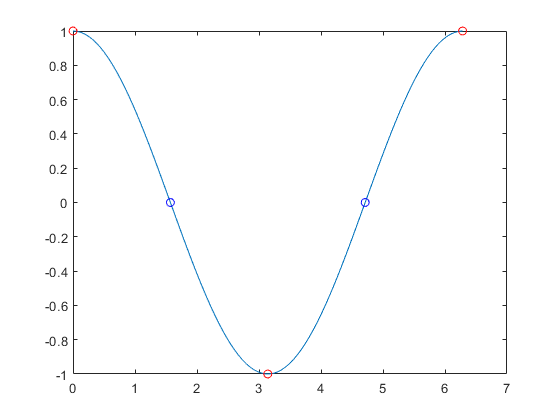
\includegraphics[width=3.5in,height=2.0in]{2_14_12_1.png}
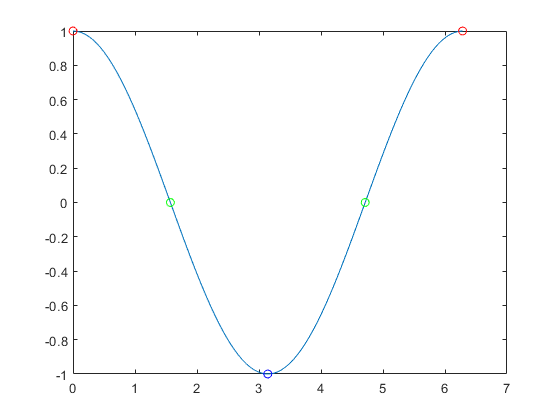
\includegraphics[width=3.5in,height=2.0in]{2_14_12_2.png}
\\
\\
{\small\bf 13}. Find the maximal and minimal curvatures of the graph $y = 1/x$.
\\
\\
{\sc Solution}: Let $f(x)=1/x$, so $f'(x)=-1/x^2$, $f''(x)=2/x^3$, and $f'''(x)=-6/x^4$. Using the formula for $\kappa'(x)$ established in Exercise 12, we have 
\begin{eqnarray*}
\kappa'(x)&=&\frac{2/x^3(-6/x^4(1+1/x^4)-3(-1/x^2)(4/x^6))}{|2/x^3|(1+1/x^4)^{5/2}} \\
&=&\frac{3|x^3|(-2/x^4(1+1/x^4)+4/x^8)}{x^3(1+1/x^4)^{5/2}} \\
&=&\frac{3|x^3|(-2/x^4+2/x^8)}{x^3(1+1/x^4)^{5/2}} \\
&=&\frac{-6|x^3|(x^4-1)}{x^3*x^8(1+1/x^4)^{5/2}}\\
&=&\frac{-6|x^3|(x^4-1)}{x^3(1+1/x^4)^{1/2}(x^4+1)^2}\\
&=&\frac{-6|x^3|(x^4-1)}{x(x^4+1)^{5/2}}
\end{eqnarray*}
It ends up being that the critical points are when $x=0,\pm 1$ (it is easy to check that $\lim_{x\rightarrow 0}\kappa'(x)=0$). We also have that
$$\kappa(x)=\frac{|2/x^3|}{(1+4/x^4)^{3/2}}$$
it ends up being that $\lim_{x\rightarrow 0}\kappa(x)=0$ and $\kappa(\pm 1)=\sqrt{2}/2$, so the maximal curvature occurs at $x=\pm 1$ and the minimal curvature at $x=0$. One could also argue that minimal curvature "occurs" ax $x$ approaches $\pm \infty$. 
\\
\\
{\small\bf 14}. Use a geometrical interpretation of the curvature to guess the point on
the graphs $y=ax^2$ and $y = ax^4$ where the maximal curvature occurs. Then verify your guess by calculations.
\\
\\
{\sc Solution}: First, $y=ax^2$ has a vertex. This intuitively seems to be where maximal curvature is (especially considering maximal curvature to be minimal radius of curvature). So our guess is at $x=0$ for $y=ax^2$. On the other hand, $y=ax^4$ is fairly flat at $x=0$ and starts to curve up on both sides. So the maximal curvature will probably occur at two points fairly close to $x=0$. To verify this, first let $f(x)=ax^2$. Then $f'(x)=2ax$, $f''(x)=2a$ (note that $|f''(x)|=f''(x)$), and $f'''(x)=0$. Then by Exercise 12, $\kappa'(x)$ is
$$\kappa'(x)=\frac{-3(2ax)(2a)^2}{(1+4a^2x^2)^{5/2}}=\frac{-24a^3x}{(1+4a^2x^2)^{5/2}}$$
Since the denominator is never $0$, the only critical point of $\kappa'(x)$ is at $x=0$. Because $\kappa'(-1)>0$ and $\kappa'(1)<0$, a sign chart reveals that this is indeed a maximum, as desired. 
\\
Next let $f(x)=ax^4$. Then $f'(x)=4ax^3$, $f''(x)=12ax^2$ (note that $|f''(x)|=f''(x)$), and $f'''(x)=24ax$. Then by Exercise 12 we have
$$\kappa'(x)=\frac{24ax(1+16ax^6)-3(4ax^3)(144a^2x^4)}{(1+16ax^6)^{5/2}}=\frac{24ax(1-56a^2x^6)}{(1+16a^2x^6)^{5/2}}$$
One critical point then is at $x=0$ whereas two more are at $x=\pm 1/(56a^2)^1/6$. A sign chart reveals that indeed, at $x=0$ curvature is minimal whereas at $x=\pm 1/(56a^2)^1/6$ curvature is maximal.
\\
\\
\noindent
{\small {\bf 15}--{\bf 17}}. Let $f(x)$ be twice continuously differentiable function and $\kappa(x)$ be the curvature of the graph $y = f(x)$.
\begin{enumerate}
  \item[{\small\bf 15}.] Does $\kappa$ attain a local maximum value at every local minimum and
maximum of $f$? If not, state an additional condition on $f$ under which the answer to this question is affirmative.
\\
\\
{\sc Solution}: By Exercise 12, we have that
$$\kappa'(x)=\frac{f''(x)(f'''(x)(1+f'(x)^2)-3f'(x)f''(x)^2)}{|f''(x)|[1+f'(x)^2]^{5/2}}$$
so long as $f''(x) \neq 0$. Suppose $f'(x_0)=0$ (i.e., there is a local min/max at $x=x_0$). Then 
$$\kappa'(x_0)=\frac{f''(x_0)f'''(x_0)}{|f''(x_0)|[1+f'(x_0)^2]^{5/2}}$$
So $\kappa'(x_0)$ may not be $0$. It will, however, always be $0$, if in addition, $f'''(x_0)=0$. 
\\
\\
  \item[{\small\bf 16}.] Prove that $\kappa=0$ at inflection points of the graph.
  \\
\\
{\sc Solution}: By definition,
$$\kappa(x)=\frac{|f''(x)|}{(1+f'(x)^2)^{3/2}}$$
Clearly if $f''(x)=0$, then $\kappa(x)=0$. So $\kappa=0$ at inflection points.
\\
\\
  \item[{\small\bf 17}.] Show by an example that the converse of the statement in Exercise
{\bf 16} is not true, i.e., that the curvature vanishes at $x = x_0$ does not
imply that the point $(x_0, f(x_0))$ is an inflection point.
\\
\\
{\sc Solution}: Consider $f(x)=1/4x^4$. Then $f'(x)=x^3$ and $f''(x)=3x^2$. Note that $f''(x) \geq 0$ for all $x$. A necessary condition for a point $x=x_0$ to be an inflection point of $f$ is that $f''(x_0)=0$; however, this is not a sufficient condition. One also needs that a change in the sign occurs, i.e., that $f''$ is positive or negative just before $x=x_0$ and negative or positive just after. So while 
$$\kappa(x)=\frac{3x^2}{(1+x^6)^{3/2}}$$
vanishes at $x=0$, the fact that there is no change in sign ($f''(x)$ is either $0$ or positive) ensures that $x=0$ is not an inflection point.
\end{enumerate}
{\small\bf 18}. Let $f$ be twice differentiable at $x_0$. Let $T_2(x)$ be its Taylor polynomial
of the second degree about $x = x_0$. Compare the curvatures of the graphs $y = f(x)$ and $y = T_2(x)$ at $x = x_0$.
\\
\\
{\sc Solution}: Recall that the second degree Taylor polynomial of $f$ about $x=x_0$ is given by
$$T_2(x)=f(x_0)+f'(x_0)(x-x_0)+\frac{1}{2}f''(x_0)(x-x_0)^2$$
The curvature for $y=f(x)$ is easy to compute, and can be verified to be
$$\kappa(x_0)=\frac{|f''(x_0)|}{(1+f'(x_0)^2)^{3/2}}$$
We have that $T_2'(x)=f'(x_0)+f''(x_0)(x-x_0)$ and $T_2''(x)=f''(x_0)$, so $T_2'(x_0)=f'(x_0)$ and $T_2''(x_0)=f''(x_0)$. Since the curvature is only dependent on the first and second derivatives, their curvatures are equal.
\\
\\
\noindent
{\small {\bf 19}--{\bf 21}}. Find the curvature of each of the following polar graphs:
\begin{enumerate}
  \item[{\small\bf 19}.] $r=1+\cos\theta$;
  \\
  \\
  {\sc Solution}: Let $r=f(\theta)$ be a polar graph. Study Problem {\bf 14.2} details that the curvature of a polar graph is
  $$\kappa(\theta)=\frac{|2f'(\theta)^2-f(\theta)f''(\theta)+f(\theta)^2|}{[f'(\theta)^2+f(\theta)^2]^{3/2}}$$
  Here, $f(\theta)=1+\cos\theta$, so $f'(\theta)=-\sin\theta$ and $f''(\theta)=-\cos\theta$. Then the curvature is
  $$\kappa(\theta)=\frac{|2(-\sin\theta)^2-(1+\cos\theta)(-\cos \theta)+(1+\cos\theta)^2|}{[(\sin\theta)^2+(1+\cos\theta)^2]^2}=\frac{3+3\cos\theta}{[2+2\cos\theta]^{3/2}}=\frac{3}{2\sqrt{2}(1+\cos\theta)^{1/2}}$$
  \item[{\small\bf 20}.] $r=e^{\theta}$;
  \\
  \\
  {\sc Solution}: We follow the same steps as above. First, let $f(\theta)=e^{\theta}$, so $f'(\theta)=e^{\theta}$ and $f''(\theta)=e^{\theta}$. Then the curvature is
  $$\kappa(\theta)=\frac{|2e^{2\theta}-e^{2\theta}+e^{2\theta}|}{(e^{2\theta}+e^{2\theta})^{3/2}}=\frac{2e^{2\theta}}{2\sqrt{2}e^{3\theta}}=\frac{1}{\sqrt{2}e^{\theta}},$$
  which was actually found in Exercise {\bf 6}. 
  \item[{\small\bf 21}.] $r=|\sin(3\theta)|$.
  \\
  \\
  {\sc Solution}: We follow the same steps as above. First, let $f(\theta)=|\sin(3\theta)|$. It is important to remember the derivative of the absolute value of a function does not exist when the function is $0$, but does exist elsewhere. It can be explicitly written as $g'(x)g(x)/|g(x)|$ if $f(x)=|g(x)|$. So,
 $$f'(\theta)=\frac{3\cos(3\theta)\sin(3\theta)}{|\sin(3\theta)|}=\frac{3\sin(6\theta)}{2|\sin(3\theta)|}$$ and 
 \begin{eqnarray*}
 f''(\theta)&=&\frac{36\cos(6\theta)|\sin(3\theta)|-6\sin(6\theta)(\frac{3\sin(6\theta)}{2|\sin(3\theta)|})}{(2|\sin(3\theta)|)^2}\\
 &=&\frac{36\cos(6\theta)|\sin(3\theta)|^2-3\sin(6\theta)(3\sin(6\theta))}{|\sin(3\theta)|(2|\sin(3\theta)|)^2}\\
  &=&\frac{36(\cos(6\theta)\sin(3\theta)^2-\sin^2(3\theta)\cos^2(3\theta))}{4\sin^2(3\theta)|\sin(3\theta)|}\\
   &=&\frac{9(\cos^2(3\theta)-\sin^2(3\theta)-\cos^2(3\theta))}{|\sin(3\theta)|}\\
   &=&\frac{-9\sin^2(3\theta)}{|\sin(3\theta)|}
 \end{eqnarray*}
 Then the curvature is
\begin{eqnarray*}
\kappa(\theta)&=&\frac{|2(\frac{3\cos(3\theta)\sin(3\theta)}{|\sin(3\theta)|})^2-(|\sin(3\theta)|)(\frac{-9\sin^2(3\theta)}{|\sin(3\theta)|})+(|\sin(3\theta)|)^2|}{((\frac{3\cos(3\theta)\sin(3\theta)}{|\sin(3\theta)|})^2+(|\sin(3\theta)|)^2)^{3/2}}\\
&=&\frac{|2(\frac{(9\cos^2(3\theta)\sin^2(3\theta))}{\sin^2(3\theta)})+9\sin^2(3\theta)+\sin^2(3\theta)|}{((\frac{(9\cos^2(3\theta)\sin^2(3\theta))}{\sin^2(3\theta)})+\sin^2(3\theta))^{3/2}}\\
&=&\frac{|2((9\cos^2(3\theta))+10\sin^2(3\theta)|}{(9\cos^2(3\theta)+\sin^2(3\theta))^{3/2}}\\
&=&\frac{|18\cos^2(3\theta)+10\sin^2(3\theta)|}{(9\cos^2(3\theta)+\sin^2(3\theta))^{3/2}}\\
&=&\frac{8\cos^2(3\theta)+10}{(8\cos^2(3\theta)+1)^{3/2}}
\end{eqnarray*}
\end{enumerate}
\noindent
{\small {\bf 22}--{\bf 26}}. Find the equation of the osculating circle for each of the following
planar curves at a specified point $P$:
\begin{enumerate}
  \item[{\small\bf 22}.] $y=x^2, \ P=(0,0)$;
  \\
  \\
  {\sc Solution}: First recall the definition of the osculating circle
  $${\bf R}(t)={\bf r}_0+\rho_0(1-\cos t)\hat{\bf N}_0+\rho_0\sin t\hat{\bf T}_0, \ \ \ 0\leq t <2\pi$$
  Thus to find the osculating circle at a point $P$, we must find $\rho_0$, $\hat{\bf N}_0$, and $\hat{\bf T}_0$. Calculation of the latter two is quite tedious for space curves; however, for planar curves (like those given), it is relatively easy. To begin with, first calculate the curvature, which is
  $$\kappa(x)=\frac{2}{(1+4x^2)^{3/2}}$$
  so the radius of curvature at $P$, $\rho_0$, is
  $$\rho_0=\rho(0)=\frac{1}{\kappa(0)}=\frac{(1+4(0)^2)^{3/2}}{2}=\frac{1}{2}$$
  Next we must find the unit normal and tangent vectors. Let the curve be parameterized by ${\bf r}(t)=\la t,f(t) \ra$. Then the unit tangent vector is given by $\hat{\bf T}(t)=1/(\sqrt{1+f'(t)^2})\la 1,f'(t) \ra$. Now we need to find the unit normal vector, which is always perpendicular to the unit tangent vector. Note that $\la -f'(t),1 \ra$ is always perpendicular to $\hat{\bf T}$; so $\hat{\bf N}=\pm1/(\sqrt{1+f'(t)^2})\la -f'(t),1 \ra$ (the appropriate sign must be chosen based on the concavity). At $t=0$, the unit normal and tangent vectors are $\hat{\bf N}_0=\la 0,1 \ra$ (positive chosen since $f$ is concave up at $t=0$) and $\hat{\bf T}_0=\la 1,0 \ra$. Therefore the osculating circle is given by
  $${\bf R}(t)=\frac{1}{2}(1-\cos t)\la 0,1 \ra+\frac{1}{2}\sin t \la 1,0 \ra = \frac{1}{2}\la \sin t, 1-\cos t \ra, \ \ \ 0\leq t <2\pi$$
  equivalently, this can be written as
  $$x^2+(y-\frac{1}{2})^2=\frac{1}{4}$$
  (an easy way to find the above is to use the general form $(x-x_0)^2+(y-y_0)^2=\rho_0^2$, where $x_0$ is the constant in the $x$ component of ${\bf R}(t)$ and $y_0$ is the constant in the $y$ component of ${\bf R}(t)$). 
  \\
  \\
  \item[{\small\bf 23}.] $y=x-x^2/4, \ P=(2,1)$;
  \\
  \\
  {\sc Solution}: As above, we begin by calculating the curvature, which is
  $$\kappa(x)=\frac{1/2}{(1+(1-x/2)^2)^{3/2}}$$
  so the radius of curvature at $P$, $\rho_0$, is
  $$\rho_0=\rho(2)=\frac{1}{\kappa(2)}=2(1+(1-2/2)^2)^{3/2}=2$$
  Next we must find the unit normal and tangent vectors. At $t=2$, the unit normal and tangent vectors are $\hat{\bf N}_0=\la 0,-1 \ra$ (negative chosen since $f$ is concave down at $t=2$) and $\hat{\bf T}_0=\la 1,0 \ra$. Therefore the osculating circle is given by
  $${\bf R}(t)=\la 2,1 \ra + 2(1-\cos t)\la 0, -1 \ra + 2\sin t \la 1,0 \ra = \la 2+2\sin t, -1+2\cos t \ra, \ \ \ 0\leq t <2\pi$$
  equivalently, this can be written as
  $$(x-2)^2+(y+1)^2=4$$
  \item[{\small\bf 24}.] $y=1/x, \ P=(1,1)$;
  \\
  \\
  {\sc Solution}: As above, we begin by calculating the curvature, which is
  $$\kappa(x)=\frac{2/x^3}{(1+(-1/x^2)^2)^{3/2}}$$
  so the radius of curvature at $P$, $\rho_0$, is
  $$\rho_0=\rho(1)=\frac{1}{\kappa(1)}=\frac{(1)^3(1+(-1/(1)^2)^2)^{3/2}}{2}=\frac{2\sqrt{2}}{2}=\sqrt{2}$$
  Next we must find the unit normal and tangent vectors. At $t=1$, the unit normal and tangent vectors are $\hat{\bf N}_0=1/\sqrt{2}\la 1,1 \ra$ (positive chosen since $f$ is concave up at $t=1$) and $\hat{\bf T}_0=1/\sqrt{2}\la 1,-1 \ra$. Therefore the osculating circle is given by
  $${\bf R}(t)=\la 1,1 \ra + \sqrt{2}(1-\cos t)(\frac{1}{\sqrt{2}})\la 1, 1 \ra + \sqrt{2}\sin t(\frac{1}{\sqrt{2}}) \la 1,-1 \ra = \la 2+\cos t +\sin t, 2+\cos t -\sin t \ra$$
  for $0\leq t <2\pi $. Equivalently, this can be written as
  $$(x-2)^2+(y-2)^2=2$$
  \item[{\small\bf 25}.] $x=a(t-\sin t),\ y=a(1-\cos t)$ (a cycloid) $P=(a(\pi/2-1),a)$;
  \\
  \\
  {\sc Solution}: As above, we begin by calculating the curvature. So $x'(t)=a(1-\cos t), \ y'(t)=a \sin t$ and $x''(t)=a \sin t, \ y''(t)=a \cos t$. Then the curvature is is
  $$\kappa(x)=\frac{|a(1-\cos t)(a \cos t)-(a \sin t)(a \sin t)|}{(a^2(1-\cos t)^2+a^2\sin^2 t)^{3/2}}=\frac{a^2|\cos t-1|}{a^3(2-2\cos t)^{3/2}}=\frac{1}{2a\sqrt{2}(1-\cos t)^{3/2}}$$
  so the radius of curvature at $P$ (which corresponds to $t=\pi/2$), $\rho_0$, is
  $$\rho_0=\rho(\pi/2)=\frac{1}{\kappa(\pi/2)}=2a\sqrt{2}(1-\cos \pi/2)^{3/2}=2a\sqrt{2}$$
  Next we must find the unit normal and tangent vectors. Note that ${\bf r}'(\pi/2)=\la a,a \ra$. So the unit tangent vector is $\hat{\bf T}_0=1/\sqrt{2}\la 1,1 \ra$. The unit normal vector must be perpendicular to this, so we have two options: $\pm 1/\sqrt{2}\la -1,1 \ra$. Choose the negative version since the curve is concave down at $t=\pi/2$. Therefore the osculating circle is given by
\begin{eqnarray*}
{\bf R}(t)&=&\la a(\pi/2-1),a \ra + 2a\sqrt{2}(1-\cos t)(\frac{1}{\sqrt{2}})\la 1, -1 \ra + 2a\sqrt{2}\sin t(\frac{1}{\sqrt{2}}) \la 1,1 \ra \\
&=& \la \frac{a\pi}{2}+a-2a\cos t + 2a\sin t, -a+2a\cos t +2a\sin t \ra, \ \ \ 0\leq t <2\pi
\end{eqnarray*}  
  equivalently, this can be written as
  $$(x-(\frac{a\pi}{2}+a))^2+(y+a)^2=8a^2$$  
  \item[{\small\bf 26}.] $x=\cos t, \ y=\sin(2t), \ P=(1,0)$ and $P=(-1,0)$.
  \\
  \\
  {\sc Solution}: I will first use $P=(1,0)$. As above, we begin by calculating the curvature. So $x'(t)=-\sin t, \ y'(t)=2\cos(2t)$ and $x''(t)=-\cos t, \ y''(t)=-4\sin(2t)$. Then the curvature is
  $$\kappa(x)=\frac{|(-\sin t)(-4\sin(2t))-(-\cos t)(2\cos(2t))|}{((-\sin t)^2+(2\cos(2t))^2)^{3/2}}=\frac{|4\sin t(\sin(2t))+2\cos t(\cos(2t))|}{(\sin^2t+4\cos^2(2t))^{3/2}}$$
  so the radius of curvature at $P$ (which corresponds to $t=0$), $\rho_0$, is
  $$\rho_0=\rho(0)=\frac{1}{\kappa(0)}=\frac{(\sin^20+4\cos^2(0))^{3/2}}{|4\sin (0)(\sin(0))+2\cos (0)(\cos(0))|}=\frac{4^{3/2}}{2}=4$$
  Next we must find the unit normal and tangent vectors. Note that ${\bf r}'(0)=\la 0,2 \ra$. So the unit tangent vector is $\hat{\bf T}_0=\la 0,1 \ra$. The unit normal vector must be perpendicular to this, so we have two options: $\pm \la 1,0 \ra$. Choose the negative version since the curve bends inward to the origin at $t=0$. Therefore the osculating circle is given by
$${\bf R}(t)=\la 1,0 \ra + 4(1-\cos t)\la -1,0 \ra + 4\sin t \la 0,1 \ra = \la -3+4\cos t,4\sin t \ra, \ \ \ 0\leq t <2\pi$$
  equivalently, this can be written as
  $$(x+3)^2+y^2=16$$  
  Now let $P=(-1,0)$, which corresponds to $t=\pi$ Then the radius of curvature, $\rho_0$, at $P$ is
  $$\rho_0=\rho(\pi)=\frac{1}{\kappa(\pi)}=\frac{(\sin^2(\pi)+4\cos^2(2\pi))^{3/2}}{|4\sin (\pi)(\sin(2\pi))+2\cos (\pi)(\cos(2\pi))|}=\frac{4^{3/2}}{2}=4$$
  Next we must find the unit normal and tangent vectors. Note that ${\bf r}'(\pi)=\la 0,2 \ra$. So the unit tangent vector is $\hat{\bf T}_0=\la 0,1 \ra$. The unit normal vector must be perpendicular to this, so we have two options: $\pm \la 1,0 \ra$. Choose the positive version since the curve bends inward to the origin at $t=0$. Therefore the osculating circle is given by
$${\bf R}(t)=\la -1,0 \ra + 4(1-\cos t)\la 1,0 \ra + 4\sin t \la 0,1 \ra = \la 3-4\cos t,4\sin t \ra, \ \ \ 0\leq t <2\pi$$
  equivalently, this can be written as
  $$(x-3)^2+y^2=16$$  
\end{enumerate}
{\small\bf 27}. Find the maximal and minimal curvature of the ellipse $x^2/a^2+y^2/b^2=1, \ a>b$ and the points where they occur. Give the equations of the osculating circles at these points.
\\
\\
{\sc Solution}: Assume $a,b$ are positive. First, the ellipse may be parameterized as ${\bf r}(t)=\la a\cos t, b\sin t\ra$. Then $x'(t)=-a\sin t, \ y'(t)= b\cos t$ and $x''(t)=-a\cos t, \ y''(t)=-b\sin t$. Then the curvature at $t$ is given by
$$\kappa(t)=\frac{|-a\sin t(-b \sin t)-b\cos t(-a\cos t)|}{(a^2\sin^2t+b^2\cos^2t)^{3/2}}=\frac{ab}{(a^2\sin^2t+b^2\cos^2t)^{3/2}}$$
Differentiating this gives
$$\kappa'(t)=\frac{-3ab(2a^2\sin t\cos t-2b^2\cos t\sin t)}{2(a^2\sin^2t+b^2\cos^2t)^{5/2}}=\frac{-3(a^2-b^2)ab\sin (2t)}{2(a^2\sin^2t+b^2\cos^2t)^{5/2}}$$
The critical points occur when $2t=0,\pi,2\pi,...$, when $t=k\pi/2$ for integers $k$. Evidently the sign of $\kappa'(t)$ depends only on $\sin (2t)$ and is in fact the same sign as $\sin (2t)$ (by assumption, $a>b$, so $a^2-b^2>0$). It can be inferred from a sign chart that the maximal $\kappa$ occur at $t=0, \pi, 2\pi, ...$ and the minimal $\kappa$ occur at $t=\pi/2, 3\pi/2, 5\pi/2,...$. These correspond to the points $(a,0)$ and $(-a,0)$ for maximal curvature and $(0,b)$ and $(0,-b)$ for minimal. The curvature at each of these points is
\begin{eqnarray*}
\kappa(0)&=&\kappa(\pi)=\frac{ab}{(a^2\sin^2(0)+b^2\cos^2(0))^{3/2}}=\frac{ab}{b^3}=\frac{a}{b^2}\\
\kappa(\frac{\pi}{2})&=&\kappa(\frac{3\pi}{2})=\frac{ab}{(a^2\sin^2(\frac{\pi}{2})+b^2\cos^2(\frac{\pi}{2}))^{3/2}}=\frac{ab}{a^3}=\frac{b}{a^2}\\
\end{eqnarray*}
Let $P=(a,0)$. The unit normal vector is $\la -1,0 \ra$ (negative since the ellipse bends in towards the origin). The center is $\rho_0=b^2/a$ units from $P$ in the direction of the unit normal vector; i.e., at $(a-b^2/a,0)$. Therefore the osculating circle is given by
$$(x-a+b^2/a)^2+y^2=\frac{b^4}{a^2}$$
Let $P=(-a,0)$. The unit normal vector is $\la 1,0 \ra$ (positive since the ellipse bends in towards the origin). The center is $\rho_0=b^2/a$ units from $P$ in the direction of the unit normal vector; i.e., at $(-a+b^2/a,0)$. Therefore the osculating circle is given by
$$(x+a-b^2/a)^2+y^2=\frac{b^4}{a^2}$$
Let $P=(0,b)$. The unit normal vector is $\la 0,-1 \ra$ (negative since the ellipse bends in towards the origin). The center is $\rho_0=a^2/b$ units from $P$ in the direction of the unit normal vector; i.e., at $(0,b-a^2/b)$. Therefore the osculating circle is given by
$$x^2+(y-b+a^2/b)^2=\frac{a^4}{b^2}$$
Let $P=(0,-b)$. The unit normal vector is $\la 0,1 \ra$ (positive since the ellipse bends in towards the origin). The center is $\rho_0=a^2/b$ units from $P$ in the direction of the unit normal vector; i.e., at $(0,-b+a^2/b)$. Therefore the osculating circle is given by
$$x^2+(y+b-a^2/b)^2=\frac{a^4}{b^2}$$
{\small\bf 28}. Let ${\bf r}(t) = \la t^3,t^2,0 \ra$ This curve is not smooth and has a cusp at $t = 0$.
Find the curvature for $t\neq 0$ and investigate its limit as $t \rightarrow 0$
\\
\\
{\sc Solution}: The curve is planar, so let $x(t)=t^3$ and $y(t)=t^2$. Then $x'(t)=3t^2, \ y'(t)=2t$ and $x''(t)=6t, \ y''(t)=2$. Then the curvature of the curve is given by
$$\kappa(t)=\frac{|3t^2(2)-6t(2t)|}{((3t^2)^2+(2t)^2)^{3/2}}=\frac{6t^2}{|t|^3(9t^2+4)^{3/2}}$$
for $t\neq 0$. We then have
\begin{eqnarray*}
\lim_{t\rightarrow 0+}\kappa(t)&=&\lim_{t\rightarrow 0+}\frac{6t^2}{t^3(9t^2+4)^{3/2}}=\lim_{t\rightarrow 0+}\frac{6}{t(9t^2+4)^{3/2}}=+\infty\\
\lim_{t\rightarrow 0-}\kappa(t)&=&\lim_{t\rightarrow 0-}\frac{6t^2}{-t^3(9t^2+4)^{3/2}}=\lim_{t\rightarrow 0-}-\frac{6}{t(9t^2+4)^{3/2}}=+\infty
\end{eqnarray*}
\\
\\
{\small\bf 29}. Show that the cardioid $r = 1 + \cos \theta$ is not smooth at the origin. Investigate
the curvature of the cardioid as the origin is approached along the
cardioid.
\\
\\
{\sc Solution}: By Exercise {\bf 19}, the curvature of the given cardiod is
$$\kappa(\theta)=\frac{3}{2\sqrt{2}(1+\cos \theta)^{1/2}}$$
The limit as $\theta$ approaches $\pi$ is $+\infty$.
\noindent
{\small {\bf 30}--{\bf 31}}. Find an equation of the osculating plane for each of the following
curves at a specified point:
\begin{enumerate}
  \item[{\small\bf 30}.] ${\bf r}(t)=\la 4t^{3/2},\ -t^2 ,\ t\ra, \ P=(4,-1,1)$;
  \\
  \\
  {\sc Solution}: Recall that the osculating circle, a planar curve, lies completely in the osculating plane. The osculating circle is also formed from a linear combination of $\hat{\bf N}_0$ and $\hat{\bf T}_0$. The latter is parallel to ${\bf r}'(t)$ while the former is a linear combination of ${\bf r}'(t)$ and ${\bf r}''(t)$ (apply product rule). Therefore the osculating plane contains the vectors ${\bf r}'(t)$ and ${\bf r}''(t)$. Therefore an equation of the osculating plane through a point $P_0$ on a curve $C$ traced by a twice differentiable function ${\bf r}(t)$, where the position vector of $P_0$ is ${\bf r}(t_0)=\la x_0,y_0,z_0 \ra$, is
  $$n_1(x-x_0)+n_2(y-y_0)+n_3(z-z_0)=0$$
  where ${\bf n}={\bf r}'(t_0)\times{\bf r}''(t_0)=\la n_1,n_2,n_3 \ra$. So we have that
  $${\bf r}'(t)=\la 6t^{1/2}, -2t, 1 \ra$$
  and
  $${\bf r}''(t)=\la 3t^{-1/2}, -2, 0 \ra$$
  The point $P=(4,-1,1)$ has position vector ${\bf r}(t_0)$ for $t_0=1$. Thus,
  $${\bf r}'(1)=\la 6,-2, 1 \ra, \ \ \  {\bf r}''(1)=\la 3,-2,0 \ra$$
  So,
  $${\bf r}'(1)\times{\bf r}''(1)=\la 2,3,-6 \ra$$
  and an equation of the osculating plane is
  $$2(x-4)+3(y+1)-6(z-1)=0 \ \Leftrightarrow \ 2x+3y-6z=-1$$
  \item[{\small\bf 31}.] ${\bf r}(t)=\la \ln t,\ \sqrt{t},\ t^2\ra, \ P=(0,1,1)$;
  \\
  \\
  {\sc Solution}: As above, we begin by computing ${\bf r}'(t)$ and ${\bf r}''(t)$. So we have that
  $${\bf r}'(t)=\la \frac{1}{t}, \frac{1}{2}t^{-1/2} , 2t\ra$$
  and
  $${\bf r}''(t)=\la -\frac{1}{t^2}, -\frac{1}{4}t^{-3/2}, 2 \ra$$
  The point $P=(0,1,1)$ has position vector ${\bf r}(t_0)$ for $t_0=1$. Thus,
  $${\bf r}'(1)=\la 1, \frac{1}{2},2 \ra, \ \ \  {\bf r}''(1)=\la -1,-\frac{1}{4},2 \ra$$
  So,
  $${\bf r}'(1)\times{\bf r}''(1)=\la \frac{3}{2},-4,\frac{1}{4} \ra$$
  and an equation of the osculating plane is
  $$\frac{3}{2}(x)-4(y-1)+\frac{1}{4}(z-1)=0 \ \Leftrightarrow \ 6z-16y+z=-15$$
\end{enumerate}
{\small\bf 32}. Find an equation for the osculating and normal planes for the curve ${\bf r}(t)=\la \ln t, 2t, t^2 \ra$ at the point $P_0$ of its intersection with the plane $y-z=1$. A plane is normal to a curve at a point if the tangent to the curve at
that point is normal to the plane.
\\
\\
{\sc Solution}: First we find the point of intersection by substituting $y(t)$ and $z(t)$ into the equation of the plane:
$$2t-t^2=1 \ \Leftrightarrow \ t^2-2t+1=0 \ \Leftrightarrow \ (t-1)^2=0 \ \Leftrightarrow \ t=1$$
And so $t_0=1$, and the point of intersection is $P=(0,2,1)$. Next we compute ${\bf r}'(t)$ and ${\bf r}''(t)$
$${\bf r}'(t)=\la \frac{1}{t}, 2, 2t \ra$$
and
$${\bf r}''(t)=\la -\frac{1}{t^2}, 0, 2 \ra$$
then at $t_0=1$,
l$${\bf r}'(1)=\la 1,2,2 \ra, \ \ \ {\bf r}''(1)=\la -1,0,2 \ra$$
therefore the normal plane is given by
$$(x-0)+2(y-2)+2(z-1)=0 \ \Leftrightarrow \ x+2y+2z=6$$
To find the osculating plane, we must find ${\bf r}'(1)\times{\bf r}''(1)$, shown below
$${\bf r}'(1)\times{\bf r}''(1)=\la 4,-4,2 \ra,$$
which is parallel to $\la 2,-2,1 \ra$. So the osculating plane is given by
$$2(x-0)-2(y-2)+(z-1)=0 \ \Leftrightarrow \ 2x-2y+z=-3$$
{\small\bf 33}. Is there a point on the curve ${\bf r}(t)=\la t,t^2,t^3 \ra$ where the osculating
plane is parallel to the plane $3x-3y+z=1$?
\\
\\
{\sc Solution}: This question is essentially asking if there exists a $t,s$ where ${\bf r}'(t)\times{\bf r}''(t)=s\la 3,-3,1 \ra$. So we must calculate the first and second derivatives, shown below:
$${\bf r}'(t)=\la 1,2t, 3t^2 \ra$$
and
$${\bf r}''(t)=\la 0,2,6t \ra$$
so ${\bf r}'(t)\times{\bf r}''(t)$ is
$${\bf r}'(t)\times{\bf r}''(t)=\la 6t^2,-6t,2 \ra=2\la 3t^2,-3t,1 \ra$$
Evidently with $t=1$ and $s=2$, it is clear that ${\bf r}'(1)\times{\bf r}''(1)$ is parallel to $\la 3,-3,1\ra$. The point is $(1,1,1)$.
\\
\\
{\small\bf 34}. Prove that the trajectory of a particle has a constant curvature if the
particle moves so that the magnitudes of its velocity and acceleration vectors
are constant.
\\
\\
{\sc Solution}: Let the trajectory of a particle be given by ${\bf r}'(t)$. Then the velocity and acceleration vectors are given by ${\bf v}(t)={\bf r}'(t)$ and ${\bf a}(t)={\bf r}''(t)$. Suppose the magnitudes of these vectors are constant; then $\|{\bf r}'(t)\|=v$ and $\|{\bf r}''(t)\|=a$ for constants $v,a$. But the curvature is given by
$$\kappa(t)=\frac{\|{\bf r}'(t)\times{\bf r}''(t)\|}{\|{\bf r}'(t)\|^3}=\frac{\|{\bf r}'(t)\|\|{\bf r}''(t)\|\sin \theta}{\|{\bf r}'(t)\|^3}=\frac{a\sin \theta}{v^2}$$
All that is left is to show that $\sin \theta$ is constant. To do this, consider ${\bf r}'(t)\cdot{\bf r}'(t)=\|{\bf r}'(t)\|^2=v^2$. Differentiating both sides yields
$${\bf r}''(t)\cdot {\bf r}'(t)+{\bf r}'(t)\cdot{\bf r}''(t)=0 \ \Leftrightarrow \ {\bf r}'(t)\cdot{\bf r}''(t)=0$$
hence $\theta=\pi/2$, and $\sin\theta=1$, a constant.
\\
\\
Alternatively, one might consider the natural parameterization of the trajectory, ${\bf r}(s)$, and simply note that $\kappa(s)=\|{\bf r}''(s)\|$, a constant, so $\kappa$ is constant.
\\
\\
{\small\bf 35}. Consider a graph $y = f(x)$ such that $f''(x_0)\neq 0$. At a point $(x_0, y_0)$ on
the curve, where $y_0 = f(x_0)$, find the equation of the osculating circle in the
form $(x-a)^2+(y-b)^2=R^2$. Hint: Show first that the vector $\la 1,f'(x_0) \ra$ is tangent to the graph and a vector orthogonal to it is $\la -f'(x_0),1 \ra$. Then
consider two cases $f''(x_0)>0$ and $f''(x_0)<0$
\\
\\
{\sc Solution}: Refer to Exercise {\bf 22} for the first part of the hint. In essence, the unit tangent vector is given by $\hat{\bf T}(t)=1/\sqrt{1+f'(t)^2}\la 1,f'(t) \ra$ and the unit normal vector is given by $\hat{\bf N}(t)=\pm 1/\sqrt{1+f'(t)^2}\la -f'(t), 1 \ra$, where plus is taken if the graph is concave up and negative is taken if the graph is concave down. We now break the problem into cases.
\\
\\
Case 1: $f''(x_0)>0$.
\\
In this case, we take $\hat{\bf N}=1/\sqrt{1+f'(t)^2}\la -f'(t), 1 \ra$. Since the graph is concave up, the osculating circle's center must lie above the curve, because we want the circle to "sit" in the graph. The center of the osculating circle is found by traveling $\rho(x_0)$ units in the direction of $\hat{\bf N}$ from $(x_0,y_0)$. In other words, the position vector of the center of the circle is
$$\la x_0,y_0 \ra + \rho(x_0)\hat{\bf N}=\la x_0 -\frac{f'(x_0)\rho(x_0)}{\sqrt{1+f'(x_0)^2}}, y_0+\frac{\rho(x_0)}{\sqrt{1+f'(x_0)^2}} \ra$$
Recall that the radius of curvature is given by
$$\rho(x)=\frac{1}{\kappa(x)}=\frac{[1+f'(x)^2]^{3/2}}{|f''(x)|}$$
at then $\rho(x_0)$ is
$$\rho(x_0)=\frac{[1+f'(x_0)^2]^{3/2}}{|f''(x_0)|}=\frac{[1+f'(x_0)^2]^{3/2}}{f''(x_0)}$$
since $f''(x_0)>0$.
Then $a=x_0-f'(x_0)(1+f'(x_0)^2)/f''(x_0)$  $b=y_0+(1+f'(x_0)^2)/f''(x_0)$, and $R^2=\rho(x_0)^2=[1+f'(x_0)^2]^3/f''(x_0)^2$. Thus the osculating circle is given by
$$(x-x_0+\frac{f'(x_0)(1+f'(x_0)^2)}{f''(x_0)})^2+(y-y_0-\frac{1+f'(x_0)^2}{f''(x_0)})^2=\frac{(1+f'(x_0)^2)^3}{f''(x_0)^2}$$
Case 2: $f''(x_0)<0$
In this case, we take $\hat{\bf N}=-1/\sqrt{1+f'(t)^2}\la -f'(t), 1 \ra$. Note that the radius of curvature will still be the same, but will have a negative sign in front (from evaluating the absolute value portion). The combination of this negative sign with that of the unit normal vector make a positive, which brings us exactly back to Case 1. The equation is the same. 
\\
\\
{\small\bf 36}. Let a smooth curve ${\bf r} = {\bf r}(t)$ be planar and lie in the $xy$ plane. At a
point $(x_0, y_0)$ on the curve, find the equation of the osculating circle in the
form $(x-a)^2+(y-b)^2=R^2$. Hint: Use the result of Study Problem {\bf 14.4} to
express the constants $a$, $b$, and $R$ via $x_0$, $y_0$, and the curvature at $(x_0, y_0)$.
\\
\\
{\sc Solution}: First, it is obvious that $R=\rho_0=1/\kappa_0$, where $\kappa_0$ is the curvature at $(x_0,y_0)$. Let ${\bf r}(t)=\la x(t),y(t),0 \ra$, where ${\bf r}(t_0)=\la x_0,y_0,0 \ra$. Then ${\bf r}'(t)=\la x'(t), y'(t), 0 \ra$ and $\hat{\bf T}(t)=1/\sqrt{x'(t)^2+y'(t)^2}\la x'(t),y'(t),0 \ra$. The unit normal vector must be orthogonal to this. So we may choose 
$$\hat{\bf N}(t)=\frac{1}{\sqrt{x'(t)^2+y'(t)^2}}\la -y'(t),x'(t),0 \ra$$
The center of the osculating circle is found by traveling $\rho_0$ units in the direction of $\hat{\bf N}_0=\hat{\bf N}(t_0)$. Recall the radius of curvature can be found using
$$\rho_0=\frac{1}{\kappa_0}=\frac{(x'(t_0)^2+y'(t_0)^2)^{3/2}}{x'(t_0)y''(t_0)-x''(t_0)y'(t_0)}$$
then the position vector of the center of the osculating circle is given by
$$\la x_0,y_0 \ra + \frac{x'(t_0)^2+y'(t_0)^2}{x'(t_0)y''(t_0)-x''(t_0)y'(t_0)}\la -y'(t_0),x'(t_0) \ra$$
So,
$$a=x_0-y'(t_0)(\frac{x'(t_0)^2+y'(t_0)^2}{x'(t_0)y''(t_0)-x''(t_0)y'(t_0)}), \ \ \ b=y_0+x'(t_0)(\frac{x'(t_0)^2+y'(t_0)^2}{x'(t_0)y''(t_0)-x''(t_0)y'(t_0)})$$
{\small\bf 36}. Find parametric equations of the osculating circle to the curve ${\bf r}(t)=\la 4t^{3/2}, -t^2, t \ra$ at the point $P = (4, -1, 1)$ by using the method of Study
Problem {\bf 14.4}.
\\
\\
{\sc Solution}: First, the point $P$ corresponds to $t=1$. We must find $\hat{\bf T}_0=\hat{\bf T}(1)$ and $\hat{\bf N}_0=\hat{\bf N}(1)$. Then,
\begin{eqnarray*}
{\bf r}'(t)&=&\la 6t^{1/2}, -2t, 1 \ra\\
\|{\bf r}'(t)\|&=&\sqrt{36t+4t^2+1}\\
\hat{\bf T}(t)&=&\frac{1}{\|{\bf r}'(t)\|}{\bf r}'(t)=\frac{1}{\sqrt{36t+4t^2+1}}\la 6t^{1/2},-2t,1 \ra \\
&\Rightarrow& \hat{\bf T}_0=\hat{\bf T}(1)=\frac{1}{\sqrt{41}}\la 6,-2,1 \ra \\
{\bf T}'(t)&=&-\frac{18+4t}{(36t+4t^2+1)^{3/2}}\la 6t^{1/2},-2t,1 \ra+\frac{1}{\sqrt{36t+4t^2+1}}\la 3t^{-1/2},-2,0 \ra \\
{\bf T}'(1)&=&-\frac{22}{41\sqrt{41}}\la 6,-2,1 \ra + \frac{41}{41\sqrt{41}}\la 3,-2,0 \ra = \frac{1}{41\sqrt{41}}\la -9,-38,-22\ra \\
&\Rightarrow& \|{\bf T}'(1)\|=\frac{1}{41\sqrt{41}}\sqrt{(-9)^2+(-38)^2+(-22)^2}=\frac{\sqrt{2009}}{41\sqrt{41}}=\frac{7}{41}\\
\hat{\bf N}_0&=&\frac{1}{\|{\bf T}'(1)\|}{\bf T}'(1)=\frac{1}{7\sqrt{41}}\la -9,-38,-22 \ra \\
\rho_0&=&\frac{1}{\kappa(1)}=\frac{\|{\bf r}'(1)\|}{\|{\bf T}'(1)\|}=\frac{\sqrt{41}}{7/41}=\frac{41\sqrt{41}}{7}
\end{eqnarray*}
The general equation of the osculating circle is
$${\bf R}(t)={\bf r}_0+\rho_0(1-\cos t)\hat{\bf N}_0+\rho_0\sin t\hat{\bf T}_0, \ 0\leq t <2\pi$$
where ${\bf r}_0=\la 4,-1,1 \ra$. Let ${\bf R}(t)=\la X(t), Y(t), Z(t) \ra$. Then
\begin{eqnarray*}
X(t)&=&4+\frac{41\sqrt{41}}{7}(1-\cos t)(-\frac{9}{7\sqrt{41}})+\frac{41\sqrt{41}}{7}\sin t(\frac{6}{\sqrt{41}})=-\frac{173}{49}+\frac{369}{49}\cos t +\frac{246}{7}\sin t \\
Y(t)&=&-1+\frac{41\sqrt{41}}{7}(1-\cos t)(-\frac{38}{7\sqrt{41}})+\frac{41\sqrt{41}}{7}\sin t(\frac{-2}{\sqrt{41}})=-\frac{1607}{49}+\frac{1558}{49}\cos t -\frac{82}{7}\sin t \\
Z(t)&=&1+\frac{41\sqrt{41}}{7}(1-\cos t)(-\frac{22}{7\sqrt{41}})+\frac{41\sqrt{41}}{7}\sin t(\frac{1}{\sqrt{41}})=-\frac{853}{49}+\frac{902}{49}\cos t +\frac{41}{7}\sin t \\
\end{eqnarray*}


\newpage
\section{Applications to Mechanics and Geometry}

\noindent
{\small {\bf 1}--{\bf 7}}. For each of the following trajectories of a particle, find the velocity,
speed, and the normal and tangential acceleration as functions of time, and their values at a specified point $P$:
\begin{enumerate}
  \item[{\small\bf 1}.] ${\bf r}(t)=\la t,\ 1-t,\ t^2+1 \ra, P=(1,0,2)$;
  \\
  \\
  {\sc Solution}: First we find the velocity and acceleration vectors
  \begin{eqnarray*}
  {\bf v}(t)&=&{\bf r}'(t)=\la 1,-1, 2t \ra\\
  {\bf a}(t)&=&{\bf r}''(t)=\la 0,0,2 \ra 
  \end{eqnarray*}
  then the speed is
  $$v(t)=\|{\bf v}(t)\|=\sqrt{1+1+4t^2}=\sqrt{2+4t^2}.$$
  Recall that the tangential and normal acceleration are given by
  \begin{eqnarray*}
  a_T(t)&=&\frac{{\bf v}(t)\cdot{\bf a}(t)}{v(t)}\\
  a_N(t)&=&\frac{\|{\bf v}(t)\times{\bf a}(t)\|}{v(t)}
\end{eqnarray*}   
Thus we have,
\begin{eqnarray*}
  a_T(t)&=&\frac{4t}{\sqrt{2+4t^2}}\\
  a_N(t)&=&\frac{\|\la -2,-2,0 \ra\|}{\sqrt{1+1+4t^2}}=\frac{2\sqrt{2}}{\sqrt{2+4t^2}}=\frac{2}{\sqrt{1+2t^2}}
\end{eqnarray*}  
The point $P=(1,0,2)$ corresponds to $t=1$. The values of the specified functions at this $t$ are
\begin{eqnarray*}
{\bf v}(1)&=&=\la 1,-1, 2 \ra\\
{\bf a}(1)&=&=\la 0,0,2 \ra \\
v(1)&=&=\sqrt{6}\\
a_T(1)&=&\frac{2\sqrt{2}}{\sqrt{3}}\\
a_N(1)&=&\frac{2}{\sqrt{3}}
\end{eqnarray*}
  \item[{\small\bf 2}.] ${\bf r}(t)=\la t^2,\ t,\ 1 \ra, P=(4,2,1)$;
  \\
  \\
  {\sc Solution}: As above, first we find the velocity and acceleration vectors
  \begin{eqnarray*}
  {\bf v}(t)&=&{\bf r}'(t)=\la 2t,1,0 \ra\\
  {\bf a}(t)&=&{\bf r}''(t)=\la 2,0,0 \ra 
  \end{eqnarray*}
  then the speed is
  $$v(t)=\|{\bf v}(t)\|=\sqrt{1+4t^2},$$
  and the tangential and normal acceleration are
\begin{eqnarray*}
  a_T(t)&=&\frac{{\bf v}(t)\cdot{\bf a}(t)}{v(t)}=\frac{4t}{\sqrt{1+4t^2}}\\
  a_N(t)&=&\frac{\|{\bf v}(t)\times{\bf a}(t)\|}{v(t)}=\frac{\|\la 0,0,-2 \ra\|}{\sqrt{1+4t^2}}=\frac{2}{\sqrt{1+4t^2}}
\end{eqnarray*}  
The point $P=(4,2,1)$ corresponds to $t=2$. The values of the specified functions at this $t$ are
\begin{eqnarray*}
{\bf v}(2)&=&\la 4,1,0 \ra\\
{\bf a}(2)&=&\la 2,0,0 \ra \\
v(2)&=&\sqrt{17}\\
a_T(2)&=&\frac{8}{\sqrt{17}}\\
a_N(2)&=&\frac{2}{\sqrt{17}}
\end{eqnarray*}
  \item[{\small\bf 3}.] ${\bf r}(t)=\la 4t^{3/2},\ -t^2,\ t\ra, P=(4,-1,1)$;
  \\
  \\
  {\sc Solution}: As above, first we find the velocity and acceleration vectors
  \begin{eqnarray*}
  {\bf v}(t)&=&{\bf r}'(t)=\la 6t^{1/2},-2t,1 \ra\\
  {\bf a}(t)&=&{\bf r}''(t)=\la 3t^{-1/2},-2,0 \ra 
  \end{eqnarray*}
  then the speed is
  $$v(t)=\|{\bf v}(t)\|=\sqrt{1+36t+4t^2},$$
  and the tangential and normal acceleration are
\begin{eqnarray*}
  a_T(t)&=&\frac{{\bf v}(t)\cdot{\bf a}(t)}{v(t)}=\frac{18+4t}{\sqrt{1+36t+4t^2}}\\
  a_N(t)&=&\frac{\|{\bf v}(t)\times{\bf a}(t)\|}{v(t)}=\frac{\|\la 2,3t^{-1/2},-6t^{1/2} \ra\|}{\sqrt{1+36t+4t^2}}=\frac{\sqrt{4+9/t+36t}}{\sqrt{1+36t+4t^2}}
\end{eqnarray*}  
The point $P=(4,-1,1)$ corresponds to $t=1$. The values of the specified functions at this $t$ are
\begin{eqnarray*}
{\bf v}(1)&=&\la 6,-2,1 \ra\\
{\bf a}(1)&=&\la 3,-2,0 \ra \\
v(1)&=&\sqrt{41}\\
a_T(1)&=&\frac{22}{\sqrt{41}}\\
a_N(1)&=&\frac{7}{\sqrt{41}}
\end{eqnarray*}
  \item[{\small\bf 4}.] ${\bf r}(t)=\la \ln t,\ \sqrt{t},\ t^2\ra, P=(0,1,1)$;
  \\
  \\
  {\sc Solution}: As above, first we find the velocity and acceleration vectors
  \begin{eqnarray*}
  {\bf v}(t)&=&{\bf r}'(t)=\la \frac{1}{t}, \frac{1}{2t^{1/2}}, 2t \ra\\
  {\bf a}(t)&=&{\bf r}''(t)=\la -\frac{1}{t^2}, -\frac{1}{4t^{3/2}}, 2 \ra 
  \end{eqnarray*}
  then the speed is
  $$v(t)=\|{\bf v}(t)\|=\sqrt{1/t^2+1/(4t)+4t^2},$$
  and the tangential and normal acceleration are
\begin{eqnarray*}
  a_T(t)&=&\frac{{\bf v}(t)\cdot{\bf a}(t)}{v(t)}=\frac{-1/t^3-1/(8t^2)+4t}{\sqrt{1/t^2+1/(4t)+4t^2}}\\
  a_N(t)&=&\frac{\|{\bf v}(t)\times{\bf a}(t)\|}{v(t)}=\frac{\|\la 3/(2t^{1/2}),-4/t,1/(4t^{5/2}) \ra\|}{\sqrt{1/t^2+1/(4t)+4t^2}}=\frac{\sqrt{9/(4t)+16/t^2+1/(16t^5)}}{\sqrt{1/t^2+1/(4t)+4t^2}}
\end{eqnarray*}  
The point $P=(0,1,1)$ corresponds to $t=1$. The values of the specified functions at this $t$ are
\begin{eqnarray*}
{\bf v}(1)&=&\la 1, \frac{1}{2}, 2 \ra\\
{\bf a}(1)&=&\la -1, -\frac{1}{4}, 2 \ra  \\
v(1)&=&\sqrt{1+1/4+4}=\frac{1}{2}\sqrt{21}\\
a_T(1)&=&\frac{23}{4\sqrt{21}}\\
\end{eqnarray*}
\begin{eqnarray*}
a_N(1)&=&\frac{\sqrt{293}}{2\sqrt{21}}
\end{eqnarray*}
  \item[{\small\bf 5}.] ${\bf r}(t)=\la \cosh t ,\ \sinh t ,\ 2+t \ra, P=(1,0,2)$;
  \\
  \\
  {\sc Solution}: As above, first we find the velocity and acceleration vectors
  \begin{eqnarray*}
  {\bf v}(t)&=&{\bf r}'(t)=\la \sinh t, \cosh t, 1 \ra\\
  {\bf a}(t)&=&{\bf r}''(t)=\la \cosh t , \sinh t, 0 \ra 
  \end{eqnarray*}
  then the speed is
  $$v(t)=\|{\bf v}(t)\|=\sqrt{\sinh^2t+\cosh^2t+1}=\sqrt{2}\cosh t,$$
  and the tangential and normal acceleration are
\begin{eqnarray*}
  a_T(t)&=&\frac{{\bf v}(t)\cdot{\bf a}(t)}{v(t)}=\frac{2\sinh t \cosh t}{\sqrt{2}\cosh t}=\sqrt{2}\sinh t\\
  a_N(t)&=&\frac{\|{\bf v}(t)\times{\bf a}(t)\|}{v(t)}=\frac{\|\la -\sinh t,\cosh t,-1 \ra\|}{\sqrt{2}\cosh t}=\frac{\sqrt{2}\cosh t}{\sqrt{2}\cosh t}=1
\end{eqnarray*}  
The point $P=(1,0,2)$ corresponds to $t=0$. The values of the specified functions at this $t$ are
\begin{eqnarray*}
{\bf v}(0)&=&\la 0, 1, 1 \ra\\
{\bf a}(0)&=&\la 1, 0, 0 \ra  \\
v(0)&=&\sqrt{2}\\
a_T(0)&=&0\\
a_N(0)&=&1
\end{eqnarray*}
  \item[{\small\bf 6}.] ${\bf r}(t)=\la e^t,\ \sqrt{2}t,\ e^{-t}\ra, P=(1,0,1)$;
  \\
  \\
  {\sc Solution}: As above, first we find the velocity and acceleration vectors
  \begin{eqnarray*}
  {\bf v}(t)&=&{\bf r}'(t)=\la e^t,\sqrt{2},-e^{-t} \ra\\
  {\bf a}(t)&=&{\bf r}''(t)=\la e^t,0,e^{-t} \ra 
  \end{eqnarray*}
  then the speed is
  $$v(t)=\|{\bf v}(t)\|=\sqrt{e^{2t}+2+e^{-2t}}=e^t+e^{-t},$$
  and the tangential and normal acceleration are
\begin{eqnarray*}
  a_T(t)&=&\frac{{\bf v}(t)\cdot{\bf a}(t)}{v(t)}=\frac{e^{2t}-e^{-2t}}{e^t+e^{-t}}=e^t-e^{-t}\\
  a_N(t)&=&\frac{\|{\bf v}(t)\times{\bf a}(t)\|}{v(t)}=\frac{\|\la \sqrt{2}e^{-t},-2,-\sqrt{2}e^t \ra\|}{e^t+e^{-t}}=\frac{\sqrt{2}(e^t+e^{-t})}{e^t+e^{-t}}=\sqrt{2}
\end{eqnarray*}  
The point $P=(1,0,1)$ corresponds to $t=0$. The values of the specified functions at this $t$ are
\begin{eqnarray*}
{\bf v}(0)&=&\la 1, \sqrt{2}, -1 \ra\\
{\bf a}(0)&=&\la 1, 0, 1 \ra  \\
v(0)&=&2\\
a_T(0)&=&0\\
a_N(0)&=&\sqrt{2}
\end{eqnarray*}
  \item[{\small\bf 7}.] ${\bf r}(t)=\la \sin t-t\cos t,\ t^2 ,\ \cos t +t\sin t \ra, P=(0,0,1)$.
  \\
  \\
  {\sc Solution}: As above, first we find the velocity and acceleration vectors
  \begin{eqnarray*}
  {\bf v}(t)&=&{\bf r}'(t)=\la t\sin t, 1, t\cos t\ra\\
  {\bf a}(t)&=&{\bf r}''(t)=\la \sin t +t\cos t,0,\cos t-t\sin t \ra 
  \end{eqnarray*}
  then the speed is
  $$v(t)=\|{\bf v}(t)\|=\sqrt{1+t^2},$$
  and the tangential and normal acceleration are
\begin{eqnarray*}
  a_T(t)&=&\frac{{\bf v}(t)\cdot{\bf a}(t)}{v(t)}=\frac{t}{\sqrt{1+t^2}}\\
  a_N(t)&=&\frac{\|{\bf v}(t)\times{\bf a}(t)\|}{v(t)}=\frac{\|\la \cos t-t\sin t,t^2,-\sin t-t\cos t \ra\|}{\sqrt{1+t^2}}=\frac{\sqrt{1+t^2+t^4}}{\sqrt{1+t^2}}
\end{eqnarray*}  
The point $P=(0,0,1)$ corresponds to $t=0$. The values of the specified functions at this $t$ are
\begin{eqnarray*}
{\bf v}(0)&=&\la 0,1,0 \ra\\
{\bf a}(0)&=&\la 0,0,1 \ra  \\
v(0)&=&1\\
a_T(0)&=&0\\
a_N(0)&=&1
\end{eqnarray*}
\end{enumerate}
{\small\bf 8}. Find the normal and tangential accelerations of a particle with the position
vector ${\bf r}(t)=\la t^2+1,t,t^2-1 \ra$ when the particle is at the least distance
from the origin.
\\
\\
{\sc Solution}: Note that the distance from the particle's position at a moment $t$ to the origin is given by $\|{\bf r}(t)\|$. The find when the distance is at a minimum, differentiate this. By Exercise {\bf 28} in section 11, we have
$$\|{\bf r}(t)\|'=\frac{{\bf r}(t)\cdot {\bf r}'(t)}{\|{\bf r}(t)\|}=\frac{{\bf r}(t)\cdot {\bf v}(t)}{\|{\bf r}(t)\|}$$
so we are looking for $t$ such that ${\bf r}(t)\cdot {\bf v}(t)=0$. We have that
\begin{eqnarray*}
{\bf v}(t)&=&\la 2t,1,2t \ra \\
{\bf a}(t)&=& \la 2,0,2 \ra
\end{eqnarray*}
Thus 
$${\bf r}(t)\cdot {\bf v}(t)=2t^3+2t+t+2t^3-2t=4t^3-t$$
which is evidently $0$ if $t=0$ or $t=\pm 1/2$. The distance to the origin is
$$\|{\bf r}(t)\|=\sqrt{2t^4+t^2+2}$$
Evidently $\|{\bf r}(1/2)\|=\|{\bf r}(-1/2)\|>\|{\bf r}(0)\|$. Thus the particle is at the least distance from the origin at $t=0$.
\\
Next, the velocity and acceleration at $t=0$ are
\begin{eqnarray*}
{\bf v}(0)&=&\la 0,1,0 \ra \\
{\bf a}(0)&=& \la 2,0,2 \ra
\end{eqnarray*}
So the speed at $t=0$ is $v(0)=1$. Then the tangential and normal accelerations are
\begin{eqnarray*}
a_T(0)&=&\frac{0}{1}=0 \\
a_N(0)&=&\frac{\|\la 2,0,-2 \ra\|}{1}=2\sqrt{2}
\end{eqnarray*}
\\
\\
{\small\bf 9}. Find the tangential and normal accelerations of a particle with the position
vector ${\bf r}(t)=\la R\sin(\omega t-\phi_0),-R\cos(\omega t-\phi_0),v_0 t\ra$ where $R$, $\omega$, $\phi_0$, and $v_0$ are constants (see Study Problem {\bf 15.4}).
\\
\\
{\sc Solution}: We have that the velocity and acceleration vectors are
\begin{eqnarray*}
{\bf v}(t)&=&\la \omega R \cos(\omega t-\phi_0), \omega R \sin(\omega t-\phi_0), v_0 \ra \\
{\bf a}(t)&=&\la -\omega^2 R \sin(\omega t-\phi_0), \omega^2 R \cos(\omega t-\phi_0), 0 \ra
\end{eqnarray*}
therefore the speed is
$$v(t)=\sqrt{\omega^2R^2+v_0^2}$$
and the tangential and normal acceleration are 
\begin{eqnarray*}
a_T(t)&=&\frac{-\omega^3R^2\sin(\omega t-\phi_0)\cos(\omega t-\phi_0)+\omega^3R^2\sin(\omega t-\phi_0)\cos(\omega t-\phi_0)}{\sqrt{\omega^2R^2+v_0^2}}=0 \\
a_N(t)&=&\frac{\|\la-v_0\omega^2R\cos(\omega t-\phi_0),-v_0\omega^2R\sin(\omega t-\phi_0),\omega^3R^2  \ra\|}{\sqrt{\omega^2R^2+v_0^2}}=\frac{\omega^2R\sqrt{v_0^2+\omega^2R^2}}{\sqrt{\omega^2R^2+v_0^2}}=\omega^2R
\end{eqnarray*}
This is essentially the general form of the converse of Study Problem {\bf 15.4}
\\
\\
{\small\bf 10}. The shape of a winding road can be approximated by the graph $y=L\cos(x/L)$, where the coordinates are in miles and $L = 1$ mile. The condition of the road is such that if the normal acceleration of a car on it exceeds $10$ m/s$^2$, the car may skid off the road. Recommend a speed limit for this portion of the road.
\\
\\
{\sc Solution}: First convert $L$ to meters, so that $y=f(x)=aL\cos(x/(aL))$, where $a=1609.34$ m/mile. Recall that
$$a_N(x)=\kappa(x)v^2=\frac{v^2}{\rho}$$
Here, $f'(x)=\sin(x/(aL))$ and $f''(x)=1/(aL)\cos(x/(aL))$. Then 
$$\kappa(x)=\frac{|\cos(x/(aL))|}{aL(1+\sin(x/(aL))^2)^{3/2}}$$
The maximal curvature occurs at $x=0$, since $\cos$ is at a maximum there and $\sin$ is at a minimum. This curvature is
$$\kappa(0)=\frac{1}{aL}$$
Let $a_m$ be the maximum normal acceleration allowed. Then a reasonable speed limit is to bound it using the maximum curvature. Thus, set 
$$a_N^{\text{max}}=a_N(0)=\kappa(0)v^2=\frac{v^2}{aL}$$
we bound this above by $a_m$, and so
$$\frac{v^2}{aL}<a_m \ \Rightarrow \ v<\sqrt{a_m(aL)}$$
note that this will have correct units, since $a_m$ is in m/s$^2$ and $aL$ is in m. So a suitable speed limit is, in m/s
$$\sqrt{a_m(aL)}=\sqrt{10(1609)}\approx 126.86$$
Conversion of this to km/h or mph yields $456.7$ km/h or $283.7$ mph
\\
\\
{\small\bf 11}. A particle moves along the curve $y=x^2+x^3$ in the direction of increasing
$x$. If the acceleration of the particle at the point $(1, 2)$ is ${\bf a} = \la -3,-1 \ra$,
find its normal and tangential accelerations.
\\
\\
{\sc Solution}: Let $f(x)=x^2+x^3$. Then ${\bf r}(t)=\la t,f(t)$ paremeterizes the curve. Thus a tangent vector to the point $(1,2)$ (corresponding to $t=1$) is 
$${\bf r}'(1)=\la 1, f'(1)\ra = \la 1,2(1)+3(1)^2 \ra = \la 1,5 \ra$$
Then the speed is $\|{\bf r}'(1)\|=\sqrt{1+25}=\sqrt{26}$. The tangential and normal accelerations are
\begin{eqnarray*}
a_T&=&\frac{\la 1,5\ra \cdot \la -3,-1 \ra}{\sqrt{26}}=-\frac{8}{\sqrt{26}}\\
a_N&=&\frac{\|\la 1,5,0 \ra \cdot \la -3,-1,0 \ra\|}{\sqrt{26}}=\frac{14}{\sqrt{26}}
\end{eqnarray*}
(note that ${\bf v}/\|{\bf v}\|$ is just the unit tangent vector, so we may choose any tangent vector to be ${\bf v}$; in particular, we have chosen ${\bf v}={\bf r}'(1)$). 
\\
\\
{\small\bf 12}. Suppose that a particle moves so that its tangential acceleration $a_T$ is
constant, while the normal acceleration $a_N$ remains $0$. What is the trajectory
of the particle?
\\
\\
{\sc Solution}: Recall that $a_T$ and $a_N$ are related by the equations
$$a_T=v', \ \ \ a_N=\kappa v^2 $$
Suppose $a_T=a$, where $a$ is a constant. Then $v'=a \ \Rightarrow v=at+v_0$ for a constant $v_0$. Suppose now that $a_N=0$. Then either $\kappa=0$ or $v^2=0$, or both. Suppose that $v=0$. Then ${\bf r}={\bf 0}$. Suppose now that $v\neq 0$. Then $\kappa=0$. Recall that straight lines have $0$ curvature.
\\
\\
{\small\bf 13}. Suppose that a particle moves so that its tangential acceleration $a_T$ remains $0$, while the normal acceleration $a_N$ is
constant. What is the trajectory
of the particle? Hint: Investigate the curvature of the trajectory
\\
\\
{\sc Solution}: As in Exercise {\bf 12}, we will need the following equations 
$$a_T=v', \ \ \ a_N=\kappa v^2 $$
Suppose $a_T=0$. Then $v'=0 \ \Rightarrow \ v=v_0$, where $v_0$ is a constant. Suppose now that $a_N$ is constant. Then $\kappa=a_n/v_0^2$ is a constant. Recall that circles have constant curvature, hence this is a circle.
\\
\\
{\small\bf 14}. A race car moves with a constant speed $v_0$ along an elliptic track $x^2/a^2+y^2/b^2=1, \ a>b$. Find the maximal and minimal values of the magnitude of its acceleration and the points where they occur.
\\
\\
{\sc Solution}: By Exercise {\bf 27} of Section 14, maximal curvature occurs at $(\pm a,0)$ and minimal curvature occurs at $(0, \pm b)$, where $\kappa^{\text{max}}=a/b^2$ and $\kappa^{\text{min}}=b/a^2$. Recall that
$$a_T=v', \ \ \ a_N=\kappa v^2$$
Since $v=v_0$, a constant, $a_T=0$. Moreover, since 
$${\bf a}(t)=a_T\hat{\bf T}+a_N\hat{\bf N}$$
where $\hat{\bf T}$ and $\hat{\bf N}$ are orthogonal, the total acceleration may be computed using the Pythagorean theorem as 
$$a=\sqrt{a_T^2+a_N^2}$$
(positive since magnitude). Hence,
$$a=\sqrt{0+a_N^2}=|a_N|=|\kappa v_0^2|$$
Thus the maximal acceleration is $av_0^2/b^2$ and the minimal acceleration is $bv_0^2/a^2$.  
\\
\\
{\small\bf 15}. Does there exist a curve with zero curvature and a non-zero torsion?
Explain the answer.
\\
\\
{\sc Solution}: Recall the Frenet-Serret equations
$$\hat{\bf T}'(s)=\kappa(s)\hat{\bf N}(s), \ \hat{\bf N}'(s)=-\kappa(s)\hat{\bf T}(s)+\tau(s)\hat{\bf B}(s), \ \hat{\bf B}'(s)=-\tau(s)\hat{\bf N}(s)$$
Suppose $\kappa(s)=0$ and $\tau(s)=\tau_0$. Then,
$$\hat{\bf T}'(s)={\bf 0}, \ \hat{\bf N}'(s)=\tau_0\hat{\bf B}(s), \ \hat{\bf B}'(s)=-\tau_0\hat{\bf N}(s)$$
Let ${\bf r}(s)$ be the natural parameterization of the curve, then ${\bf r}'(s)=\hat{\bf T}(s)$, and so ${\bf r}''(s)=\hat{\bf T}'(s)={\bf 0}$. Integration of this gives ${\bf r}(s)=r_0+\hat{\bf T}_0s$ where ${\bf r}_0$ and $\hat{\bf T}_0$ are constant vectors with $\hat{\bf T}(s)=\hat{\bf T}_0$, so a curve does exist and it is a straight line. Take the derivative of both sides of the second equation and substitute $\hat{\bf B}'(s)$ into the third. This yields
$$1/\tau_0\hat{\bf N}''(s)=-\tau_0\hat{\bf N}(s)$$
Let $x(t)$ be one component of $\hat{\bf N}(s)$. Then we have
$$x(t)=-\frac{1}{\tau_0^2}x''(t)$$
Suppose $x(t)=A\cos(\tau_0s)+B\sin(\tau_0t)$. Then,
$$A\cos(\tau_0s)+B\sin(\tau_0s)=-\frac{1}{\tau_0^2}(-A\tau_0^2\cos(\tau_0s)-B\tau_0^2\sin(\tau_0s))=A\cos(\tau_0s)+B\sin(\tau_0s)$$
which is true for any choice of $A,B$. Then,
$$\hat{\bf N}(s)=\cos(\tau_0s){\bf u}+\sin(\tau_0s){\bf v}$$
for constant vectors ${\bf u}, {\bf v}$. Substituting $s=0$ yields
$$\hat{\bf N}_0=\hat{\bf N}(0)={\bf u}$$
Taking the derivative of this gives
$$\hat{\bf N}'(s)=-\tau_0\sin(\tau_0s)\hat{\bf N}_0+\tau_0\cos(\tau_0s){\bf v}=\tau_0\hat{\bf B}(s)$$
And so,
$$\hat{\bf B}(s)=-\sin(\tau_0s)\hat{\bf N}_0+\cos(\tau_0s){\bf v}$$
Substitution of $s=0$ yields
$$\hat{\bf B}_0=\hat{\bf B}(s)={\bf v}$$
and so
\begin{eqnarray*}
\hat{\bf N}(s)&=&\cos(\tau_0s)\hat{\bf N}_0+\sin(\tau_0s)\hat{\bf B}_0 \\
\hat{\bf B}(s)&=&\cos(\tau_0s)\hat{\bf B}_0-\sin(\tau_0s)\hat{\bf N}_0
\end{eqnarray*}
which describes a rotation (note the resemblance to the rotation matrix!)
So, as $s$ increases, $\hat{\bf N}(s)$ and $\hat{\bf B}(s)$ rotate around the line, hence a nonzero torsion. 
\noindent
{\small {\bf 16}--{\bf 20}}. For each of the following curves, find the unit tangent, normal, and
binormal vectors and the torsion at a specified point $P$:
\begin{enumerate}
  \item[{\small\bf 16}.] ${\bf r}(t)=\la t,\ 1-t,\ t^2+1\ra, \ P=(1,0,2)$;
  \\
  \\
  {\sc Solution}: First recall the equations for the unit tangent, normal, and binormal vectors, and  torsion:
  \begin{eqnarray*}
  \hat{\bf T}(t_0)&=&\frac{{\bf r}'(t_0)}{\|{\bf r}'(t_0)\|} \\
  \hat{\bf B}(t_0)&=&\frac{{\bf r}'(t_0)\times{\bf r}''(t_0)}{\|{\bf r}'(t_0)\times{\bf r}''(t_0)\|} \\
  \hat{\bf N}(t_0)&=&\hat{\bf B}(t_0)\times\hat{\bf T}(t_0) \\
  \tau(t_0)&=&\frac{{\bf r}'''(t_0)\cdot({\bf r}'(t_0)\times{\bf r}''(t_0))}{\|{\bf r}'(t_0)\times{\bf r}''(t_0)\|^2}
  \end{eqnarray*}
  So we must first find ${\bf r}'(t_0)$, ${\bf r}''(t_0)$, and ${\bf r}'''(t_0)$. The given point corresponds to $t_0=1$. So,
  \begin{eqnarray*}
  {\bf r}'(t)&=&\la 1,-1, 2t \ra \ \Rightarrow \ {\bf r}'(1)=\la 1,-1, 2 \ra \\
  {\bf r}''(t)&=&\la 0,0,2 \ra \ \Rightarrow \ {\bf r}''(1)=\la 0,0,2 \ra \\
  {\bf r}'''(t)&=&\la 0,0,0 \ra  \ \Rightarrow \ {\bf r}'''(1)={\bf 0}
  \end{eqnarray*}
  Thus we have
  \begin{eqnarray*}
  \hat{\bf T}(1)&=&\frac{\la 1,-1, 2 \ra}{\|\la 1,-1, 2 \ra\|}=\frac{1}{\sqrt{6}}\la 1,-1,2 \ra \\
  \hat{\bf B}(1)&=&\frac{\la -2,-2,0 \ra}{\|\la -2,-2,0 \ra\|}=\frac{1}{\sqrt{2}}\la -1,-1,0 \ra \\
  \hat{\bf N}(1)&=&\frac{1}{\sqrt{2}\sqrt{6}} \la -1,-1,0 \ra\times\la 1,-1,2 \ra=\frac{1}{2\sqrt{3}}\la -2,2,2 \ra= \frac{1}{\sqrt{3}}\la -1,1,1 \ra\\
  \tau(1)&=&\frac{{\bf 0}\cdot(\la -1,-1,0 \ra)}{\sqrt{2}^2}=0
  \end{eqnarray*}  
  \item[{\small\bf 17}.] ${\bf r}(t)=\la t^3,\ t^2,\ 1\ra, \ P=(8,4,1)$;
  \\
  \\
  {\sc Solution}: As above, we must first find ${\bf r}'(t_0)$, ${\bf r}''(t_0)$, and ${\bf r}'''(t_0)$. The given point corresponds to $t_0=2$. So,
  \begin{eqnarray*}
  {\bf r}'(t)&=&\la 3t^2,2t,0 \ra \ \Rightarrow \ {\bf r}'(2)=\la 12,4,0 \ra \\
  {\bf r}''(t)&=&\la 6t,2,0 \ra \ \Rightarrow \ {\bf r}''(2)=\la 12,2,0 \ra \\
  {\bf r}'''(t)&=&\la 6,0,0 \ra  \ \Rightarrow \ {\bf r}'''(2)=\la 6,0,0 \ra
  \end{eqnarray*}
  Thus we have
  \begin{eqnarray*}
  \hat{\bf T}(2)&=&\frac{\la 12,4,0 \ra}{\|\la 12,4,0 \ra\|}=\frac{1}{\sqrt{10}}\la 3,1,0 \ra \\
  \hat{\bf B}(2)&=&\frac{\la 0,0,-24 \ra}{\|\la 0,0,-24 \ra\|}= \la 0,0,-1 \ra \\
  \hat{\bf N}(2)&=&\frac{1}{\sqrt{10}} \la 0,0,-1 \ra\times\la 3,1,0 \ra=\frac{1}{\sqrt{10}}\la 1,-3,0 \ra \\
  \tau(2)&=&\frac{\la 6,0,0 \ra\cdot(\la 0,0,-1 \ra)}{1^2}=0
  \end{eqnarray*} 
  \item[{\small\bf 18}.] ${\bf r}(t)=\la 4t^{3/2},\ -t^2,\ t\ra, \ P=(4,-1,1)$;
  \\
  \\
  {\sc Solution}: As above, we must first find ${\bf r}'(t_0)$, ${\bf r}''(t_0)$, and ${\bf r}'''(t_0)$. The given point corresponds to $t_0=1$. So,
  \begin{eqnarray*}
  {\bf r}'(t)&=&\la 6t^{1/2},-2t,1 \ra \ \Rightarrow \ {\bf r}'(1)=\la 6,-2,1 \ra \\
  {\bf r}''(t)&=&\la 3t^{-1/2},-2,0 \ra \ \Rightarrow \ {\bf r}''(1)=\la 3,-2,0 \ra \\
  {\bf r}'''(t)&=&\la -3/2t^{-3/2},0,0 \ra  \ \Rightarrow \ {\bf r}'''(1)=\la -3/2,0,0 \ra
  \end{eqnarray*}
  Thus we have
  \begin{eqnarray*}
  \hat{\bf T}(1)&=&\frac{\la 6,-2,1 \ra}{\|\la 6,-2,1 \ra\|}=\frac{1}{\sqrt{41}}\la 6,-2,1 \ra \\
  \hat{\bf B}(1)&=&\frac{\la 2,3,-6 \ra}{\|\la 2,3,-6 \ra\|}= \frac{1}{7}\la 2,3,-6 \ra \\
  \hat{\bf N}(1)&=&\frac{1}{7\sqrt{41}} \la 2,3,-6 \ra\times\la 6,-2,1 \ra=\frac{1}{7\sqrt{41}}\la -9,-38,22 \ra \\
  \tau(1)&=&\frac{\la -3/2,0,0 \ra\cdot(\la 2,3,-6 \ra)}{7^2}=-\frac{3}{49}
  \end{eqnarray*} 
  \item[{\small\bf 19}.] ${\bf r}(t)=\la \ln t,\ 2\sqrt{t},\ t^2\ra, \ P=(0,2,1)$;
  \\
  \\
  {\sc Solution}: As above, we must first find ${\bf r}'(t_0)$, ${\bf r}''(t_0)$, and ${\bf r}'''(t_0)$. The given point corresponds to $t_0=1$. So,
  \begin{eqnarray*}
  {\bf r}'(t)&=&\la \frac{1}{t},t^{-1/2},2t \ra \ \Rightarrow \ {\bf r}'(1)=\la 1,1,2 \ra \\
  {\bf r}''(t)&=&\la -\frac{1}{t^2},-\frac{1}{2}t^{-3/2},2 \ra \ \Rightarrow \ {\bf r}''(1)=\la -1,-\frac{1}{2},2 \ra \\
  {\bf r}'''(t)&=&\la \frac{2}{t^3},\frac{3}{4}t^{-5/2},0 \ra  \ \Rightarrow \ {\bf r}'''(1)=\la 2,\frac{3}{4},0 \ra
  \end{eqnarray*}
  Thus we have
  \begin{eqnarray*}
  \hat{\bf T}(1)&=&\frac{\la 1,1,2 \ra}{\|\la 1,1,2 \ra\|}=\frac{1}{\sqrt{6}}\la 1,1,2 \ra \\
  \hat{\bf B}(1)&=&\frac{\la 3,-4,1/2 \ra}{\|\la 3,-4,1/2 \ra\|}= \frac{2}{\sqrt{101}}\la 3,-4,1/2 \ra=\frac{1}{\sqrt{101}}\la 6,-8,1 \ra \\
  \hat{\bf N}(1)&=&\frac{1}{\sqrt{101}\sqrt{6}} \la 6,-8,1 \ra\times\la 1,1,2 \ra=\frac{1}{\sqrt{606}}\la -17,-11,14 \ra \\
  \tau(1)&=&\frac{\la 2,\frac{3}{4},0 \ra\cdot(\la 3,-4,1 \ra)}{\sqrt{101}^2/2^2}=\frac{4(6-3)}{101}=\frac{12}{101}
  \end{eqnarray*} 
  It is important to use the non-simplified form of the cross product, because its magnitude must be squared.
  \\
  \\
  \item[{\small\bf 20}.] ${\bf r}(t)=\la \cosh t,\ \sinh t,\ 2+t\ra, \ P=(1,0,2)$.
  \\
  \\
  {\sc Solution}: As above, we must first find ${\bf r}'(t_0)$, ${\bf r}''(t_0)$, and ${\bf r}'''(t_0)$. The given point corresponds to $t_0=0$. So,
  \begin{eqnarray*}
  {\bf r}'(t)&=& \la \sinh t, \cosh t, 1 \ra \ \Rightarrow \ {\bf r}'(0)=\la 0,1,1 \ra \\
  {\bf r}''(t)&=&\la \cosh t,\ \sinh t,\ 0\ra \ \Rightarrow \ {\bf r}''(0)=\la 1,0,0 \ra \\
  {\bf r}'''(t)&=&\la \sinh t, \cosh t, 0 \ra  \ \Rightarrow \ {\bf r}'''(0)=\la 0,1,0 \ra
  \end{eqnarray*}
  Thus we have
  \begin{eqnarray*}
  \hat{\bf T}(0)&=&\frac{\la 0,1,1 \ra}{\|\la 0,1,1 \ra\|}=\frac{1}{\sqrt{2}}\la 0,1,1 \ra \\
  \hat{\bf B}(0)&=&\frac{\la 0,1,-1 \ra}{\|\la 0,1,-1 \ra\|}= \frac{1}{\sqrt{2}}\la 0,1,-1 \ra \\
  \hat{\bf N}(0)&=&\frac{1}{\sqrt{2}\sqrt{2}} \la 0,1,-1 \ra\times\la 0,1,1 \ra=\frac{1}{2}\la 2,0,0 \ra=\la 1,0,0 \ra \\
  \tau(0)&=&\frac{\la 0,1,0 \ra\cdot(\la 0,1,-1 \ra)}{\sqrt{2}^2}=\frac{1}{2}
  \end{eqnarray*} 
\end{enumerate}
{\small\bf 21}. Let ${\bf r}(t)=\la \cos t+t\sin t,\sin t-t\cos t, t^2 \ra$. Find the speed, the tangential and normal accelerations, the curvature and torsion, and the unit tangent
vector, normal, and binormal as functions of time $t$.
Hint: To simplify calculations, find the decomposition ${\bf r}(t)={\bf v}(t)-t{\bf w}(t)+t^2\hat{\bf e}_3$ where $\bf v$, $\bf w$, and $\hat{\bf e}_3$ are mutually orthogonal unit vectors such that ${\bf v}'(t)={\bf w}(t), \ {\bf w}'(t)=-{\bf v}(t)$. Use the properties of the cross products of mutually orthogonal unit vectors.
\\
\\
{\sc Solution}: Let 
$${\bf r}(t)=\la \cos t+t\sin t,\sin t-t\cos t, t^2 \ra=\la \cos t, \sin t, 0 \ra-t\la -\sin t, \cos t,0 \ra +t^2\la 0,0,1 \ra$$
Then ${\bf v}(t)=\la \cos t, \sin t, 0 \ra$ and ${\bf w}(t)=\la -\sin t, \cos t,0 \ra $. It should be evident that these satisfy the conditions in the hint. So,
\begin{eqnarray*}
{\bf r}'(t)&=&{\bf v}'(t)-{\bf w}(t)-t{\bf w}'(t)+2t\hat{\bf e}_3={\bf w}(t)-{\bf w}(t)+t{\bf v}(t)+2t\hat{\bf e}_3=t{\bf v}(t)+2t\hat{\bf e}_3 \\
{\bf r}''(t)&=&{\bf v}(t)+t{\bf v}'(t)+2\hat{\bf e}_3 ={\bf v}(t)+t{\bf w}(t)+2\hat{\bf e}_3 \\
{\bf r}'''(t)&=&{\bf v}'(t)+{\bf w}(t)+t{\bf w}'(t)=2{\bf w}(t)-t{\bf v}(t)
\end{eqnarray*}
Since ${\bf v}(t)$ and $\hat{\bf e}_3$ are orthogonal, the speed may be calculated using the Pythagorean theorem, shown below
$$v(t)=|t|\sqrt{1+4}=\sqrt{5}|t|$$
The dot product ${\bf r}'(t)\cdot{\bf r}''(t)$ is
\begin{eqnarray*}
{\bf r}'(t)\cdot{\bf r}''(t)&=&t({\bf v}(t)+2\hat{\bf e}_3)\cdot({\bf v}(t)+t{\bf w}(t)+2\hat{\bf e}_3)=t[{\bf v}(t)\cdot{\bf v}(t)+4\hat{\bf e}_3\cdot \hat{\bf e}_3]\\
&=&t[\|{\bf v}(t)\|^2+4\|\hat{\bf e}_3\|^2]=5t
\end{eqnarray*}
owing to the orthogonality of ${\bf v}(t)$, ${\bf w}(t)$, and $\hat{\bf e}_3$, and the fact that each of those vectors is a unit vector. 
\\
The cross product ${\bf r}'(t)\times{\bf r}''(t)$ is
\begin{eqnarray*}
{\bf r}'(t)\times{\bf r}''(t)&=&t({\bf v}(t)+2\hat{\bf e}_3)\times({\bf v}(t)+t{\bf w}(t)+2\hat{\bf e}_3)\\
&=&t[t{\bf v}(t)\times{\bf w}(t)+2{\bf v}(t)\times\hat{\bf e}_3+2\hat{\bf e}_3\times{\bf v}(t)+2t\hat{\bf e}_3\times{\bf w}(t)]\\
&=&t^2[{\bf v}(t)\times{\bf w}(t)+2\hat{\bf e}_3\times{\bf w}(t)] \\
&=&t^2[\hat{\bf e}_3-2{\bf v}(t)] 
\end{eqnarray*}
(the cross products can be easily calculated by imagining ${\bf v}(t)$ as $\hat{\bf e}_1$ and ${\bf w}(t)$ as $\hat{\bf e}_2$). The magnitude of the cross product is easily found using the Pythagorean theorem, shown below:
$$\|{\bf r}'(t)\times{\bf r}''(t)\|=t^2\sqrt{1+4}=\sqrt{5}t^2$$
The cross product $({\bf r}'(t)\times{\bf r}''(t))\times({\bf r}'(t))$ is
\begin{eqnarray*}
({\bf r}'(t)\times{\bf r}''(t))\times({\bf r}'(t))&=&t^2[\hat{\bf e}_3-2{\bf v}(t)] \times(t)({\bf v}(t)+2\hat{\bf e}_3) \\
&=&t^3[\hat{\bf e}_3\times{\bf v}(t)-4{\bf v}(t)\times\hat{\bf e}_3] \\
&=&t^3[5\hat{\bf e}_3\times{\bf v}(t)]=5t^3{\bf w}(t)
\end{eqnarray*}
Finally, the triple product $ {\bf r}'''(t)\cdot({\bf r}'(t)\times{\bf r}''(t))$ is
\begin{eqnarray*}
{\bf r}'''(t)\cdot({\bf r}'(t)\times{\bf r}''(t))&=&(2{\bf w}(t)-t{\bf v}(t))\cdot(t^2[\hat{\bf e}_3-2{\bf v}(t)]) \\
&=&t^2[-2(-t){\bf v}(t)\cdot{\bf v}(t)]=2t^3
\end{eqnarray*}
Then we have the tangential acceleration, normal acceleration, unit tangent vector, unit binormal vector, unit normal vector, and torsion are:
\begin{eqnarray*}
a_T(t)&=&\frac{{\bf r}'(t)\cdot{\bf r}''(t)}{\|{\bf r}'(t)\|}=\frac{5t}{\sqrt{5}|t|}=\frac{\sqrt{5}t}{|t|} \\
a_N(t)&=&\frac{{\bf r}'(t)\times{\bf r}''(t)}{\|{\bf r}'(t)\|}=\frac{\sqrt{5}t^2}{\sqrt{5}|t|}=\frac{t^2}{|t|}=|t| \\
\hat{\bf T}(t)&=&\frac{{\bf r}'(t)}{\|{\bf r}'(t)\|}=\frac{1}{\sqrt{5}|t|}[t({\bf v}(t)+2\hat{\bf e}_3)]=\frac{|t|}{t\sqrt{5}}({\bf v}(t)+2\hat{\bf e}_3)\\
\hat{\bf B}(t)&=&\frac{{\bf r}'(t)\times{\bf r}''(t)}{\|{\bf r}'(t)\times{\bf r}''(t)\|}=\frac{1}{\sqrt{5}t^2}[t^2(\hat{\bf e}_3-2{\bf v}(t))]=\frac{1}{\sqrt{5}}(\hat{\bf e}_3-2{\bf v}(t))\\
\hat{\bf N}(t)&=&\hat{\bf B}(t)\times\hat{\bf T}(t)=\frac{[{\bf r}'(t)\times{\bf r}''(t)]\times{\bf r}'(t)}{\|{\bf r}'(t)\times{\bf r}''(t)\|\|{\bf r}'(t)\|}=\frac{5t^3{\bf w}(t)}{\sqrt{5}t^2\sqrt{5}|t|}=\frac{|t|}{t}{\bf w}(t)\\
\tau(t)&=&\frac{{\bf r}'''(t)\cdot({\bf r}'(t)\times{\bf r}''(t))}{\|{\bf r}'(t)\times{\bf r}''(t)\|^2}=\frac{2t^3}{(\sqrt{5}t^2)^2}=\frac{2t^3}{5t^4}=\frac{2}{5t}
\end{eqnarray*}
\\
\\
{\small\bf 22}. Let $C$ be the curve of intersection of an ellipsoid $x^2/a^2+y^2/b^2+z^2/c^2=1$ with the plane $2x-2y+z=0$. Find the torsion and the binormal $\hat{\bf B}$ along $C$.
\\
\\
{\sc Solution}: Planar curves have a torsion of $0$, so $\tau=0$. Let ${\bf r}(t)$ parameterize the curve. Recall that the osculating plane at a point with position vector ${\bf r}(t_0)$ has a normal vector of ${\bf r}'(t_0)\times{\bf r}''(t_0)$. But $\hat{\bf B}(t_0)={\bf r}'(t_0)\times{\bf r}''(t_0)/\|{\bf r}'(t_0)\times{\bf r}''(t_0)\|$. So 
$$\hat{\bf B}=\frac{\la 2,-2,1 \ra}{\|\la 2,-2,1 \ra\|}=\frac{1}{3}\la 2,-2,1 \ra$$


\chapter{Differentiation of Multivariable  Functions}
\section{Functions of Several Variables}
\noindent
{\small {\bf 1}--{\bf 13}}. Find and sketch the domain of each of the following functions:
\begin{enumerate}
  \item[{\small\bf 1}.] $f(x,y)=x/y$.
  \\
  \\
  {\sc Solution}: Recall that the domain of a function is, in essence, the set of $n-$tuples such that $f$ is able to assign a value to each. Therefore, a strategy for finding the domain is to take the set of all $n-$tuples (i.e., $\mathbb{R}^n$) and remove from this those $n-$tuples that $f$ cannot assign a value to (so-called "problem points"). The easiest way to do this is to break $f$ into the sum and product of other simpler functions, find the domain of each of these, and take the intersection of them. The intersection will be the domain of $f$. For example, here the only issue is when $y=0$, because $1/y$ is not defined there. So the domain of $f$ is
  $$D=\{(x,y)\in \mathbb{R}^2 \ | \ y\neq 0 \}$$ 
  a sketch is
  \begin{center}
  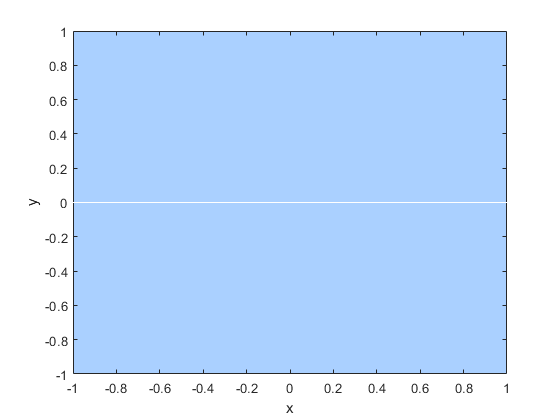
\includegraphics[width=3.5in,height=2.0in]{3_1_1.png}
  \end{center}
  on the unit square, where blue represents points in the domain of $f$ and white those that are not. 
  \\
  \\
  \item[{\small\bf 2}.] $f(x,y)=x/(x^2+y^2)$.
  \\
  \\
  {\sc Solution}: As above, we begin by finding the "problem points". Here, the only issue is when $x^2+y^2=0$, because $1/(x^2+y^2)$ is not defined there. So the domain of $f$ is
  $$D=\{(x,y)\in \mathbb{R}^2 \ | \ x\neq 0 \ \text{and} \ y\neq 0  \}$$ 
  a sketch is
  \begin{center}
  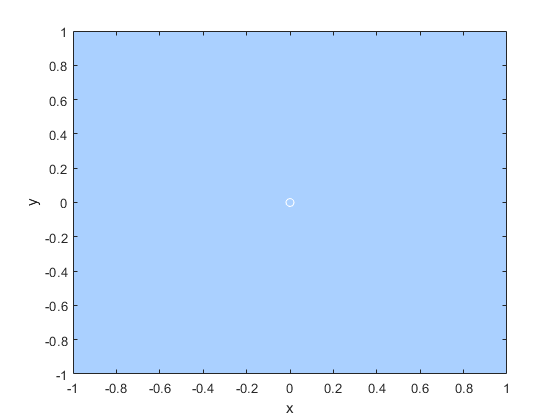
\includegraphics[width=3.5in,height=2.0in]{3_1_2.png}
  \end{center}
  on the unit square, where blue represents points in the domain of $f$ and white those that are not. 
  \\
  \\
  \item[{\small\bf 3}.] $f(x,y)=x/(y^2-4x^2)$.
  \\
  \\
  {\sc Solution}: As above, we begin by finding the "problem points". Here, the only issue is when $y^2-4x^2=0 \ \Leftrightarrow \ y=\pm 2x$, because $1/(y^2-4x^2)$ is not defined there. So the domain of $f$ is
  $$D=\{(x,y)\in \mathbb{R}^2 \ | y\neq\pm 2x  \}$$ 
  a sketch is
  \begin{center}
  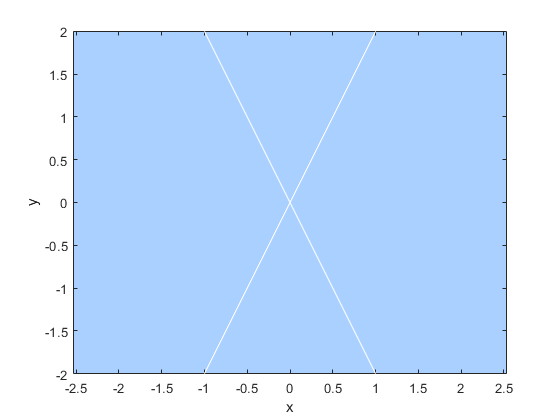
\includegraphics[width=3.5in,height=2.0in]{3_1_3.png}
  \end{center}
  where blue represents points in the domain of $f$ and white those that are not. 
  \\
  \\
  \item[{\small\bf 4}.] $f(x,y)=\ln(9-x^2-(y/2)^2)$.
  \\
  \\
  {\sc Solution}: As above, we begin by finding the "problem points". Here, the only issue is when $9-x^2-(y/2)^2 \leq 0 \ \Leftrightarrow \ 9 \leq x^2+y^2/4 \ \Leftrightarrow \ 1\geq x/9+y^2/36$, because $\ln(9-x^2-(y/2)^2)$ is not defined there. So the domain of $f$ is
  $$D=\{(x,y)\in \mathbb{R}^2 \ |  x/9+y^2/36<1 \}$$ 
  a sketch is
  \begin{center}
  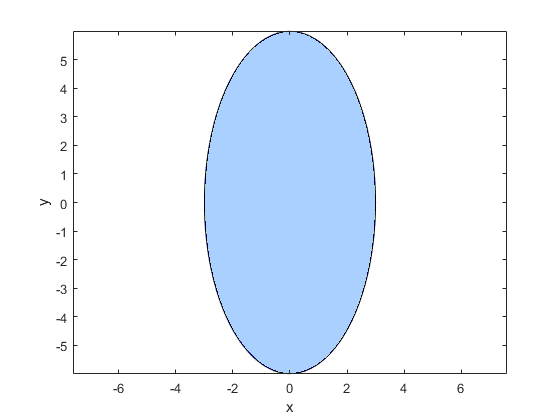
\includegraphics[width=3.5in,height=2.0in]{3_1_4.png}
  \end{center}
  where blue represents points in the domain of $f$ and white those that are not (note: the border of the ellipse is not included!). 
  \\
  \\
  \item[{\small\bf 5}.] $f(x,y)=\sqrt{1-(x/2)^2-(y/3)^2}$.
  \\
  \\
  {\sc Solution}: As above, we begin by finding the "problem points". Here, the only issue is when $1-(x/2)^2-(y/3)^2 < 0 \ \Leftrightarrow \ 1 < x^2/4+y^2/9$, because $\sqrt{1-(x/2)^2-(y/3)^2}$ is not defined there. So the domain of $f$ is
  $$D=\{(x,y)\in \mathbb{R}^2 \ |  x/4+y^2/9 \leq 1 \}$$ 
  a sketch is
  \begin{center}
  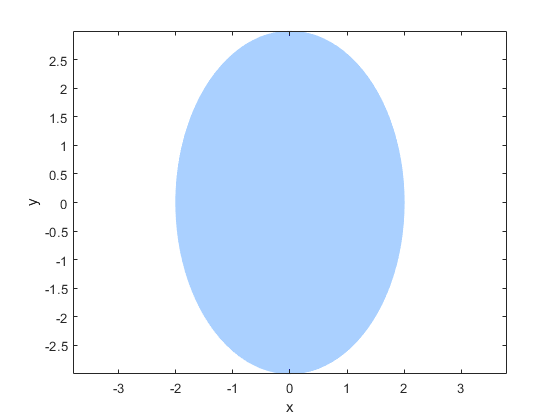
\includegraphics[width=3.5in,height=2.0in]{3_1_5.png}
  \end{center}
  where blue represents points in the domain of $f$ and white those that are not (note: the border of the ellipse is included!). 
  \\
  \\
  \item[{\small\bf 6}.] $f(x,y)=\sqrt{4-x^2-y^2}+2x\ln y$.
  \\
  \\
  {\sc Solution}: As above, we begin by finding the "problem points". Here, we have two simple functions to consider; the square root and the logarithm. $\sqrt{4-x^2-y^2}$ is not defined whenever $4-x^2-y^2 <0 \ \Leftrightarrow \ 4<x^2+y^2$. $\ln y$ is not defined whenever $y \leq 0$. So the domain of $f$ is
  $$D=\{(x,y)\in \mathbb{R}^2 \ |  x^2+y^2 \leq 4, y>0\}$$ 
  a sketch is
  \begin{center}
  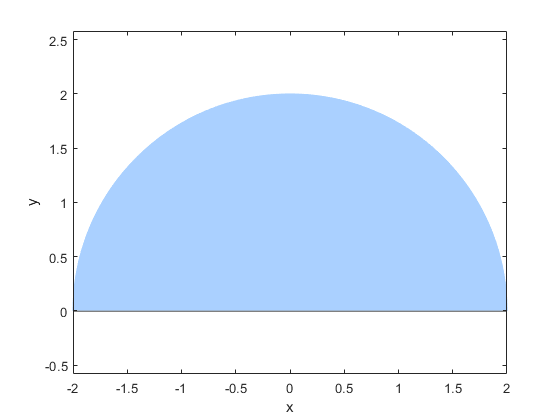
\includegraphics[width=3.5in,height=2.0in]{3_1_6.png}
  \end{center}
  where blue represents points in the domain of $f$ and white those that are not (note: the bottom border of the circle is not included, but the rest is!). 
  \\
  \\
  \item[{\small\bf 7}.] $f(x,y)=\sqrt{4-x^2-y^2}+x\ln y^2$.
  \\
  \\
  {\sc Solution}: As above, we begin by finding the "problem points". Here, we have two simple functions to consider; the square root and the logarithm. $\sqrt{4-x^2-y^2}$ is not defined whenever $4-x^2-y^2 <0 \ \Leftrightarrow \ 4<x^2+y^2$. $\ln y^2$ is not defined whenever $y^2 \leq 0 \ \Leftrightarrow \ y=0$. So the domain of $f$ is
  $$D=\{(x,y)\in \mathbb{R}^2 \ |  x^2+y^2 \leq 4, y\neq 0\}$$ 
  a sketch is
  \begin{center}
  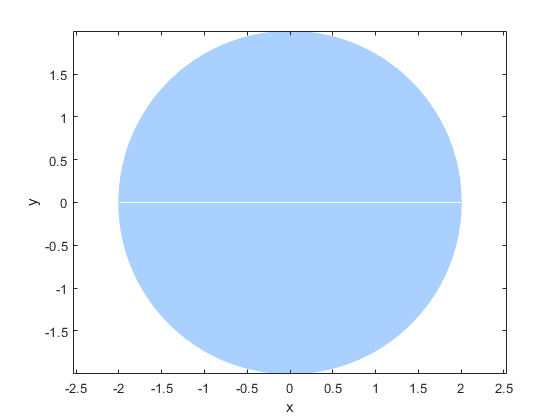
\includegraphics[width=3.5in,height=2.0in]{3_1_7.png}
  \end{center}
  where blue represents points in the domain of $f$ and white those that are not (note: entire border  is included, except when $y=0$!). 
  \\
  \\
  \item[{\small\bf 8}.] $f(x,y)=\sqrt{4-x^2-y^2}+\ln (x^2+y^2-1)$.
  \\
  \\
  {\sc Solution}: As above, we begin by finding the "problem points". Here, we have two simple functions to consider; the square root and the logarithm. $\sqrt{4-x^2-y^2}$ is not defined whenever $4-x^2-y^2 <0 \ \Leftrightarrow \ 4<x^2+y^2$. $\ln (x^2+y^2-1)$ is not defined whenever $x^2+y^2-1 \leq 0 \ \Leftrightarrow \ x^2+y^2 \leq 1$. So the domain of $f$ is
  $$D=\{(x,y)\in \mathbb{R}^2 \ |  x^2+y^2 \leq 4, x^2+y^2>1\}$$ 
  a sketch is
  \begin{center}
  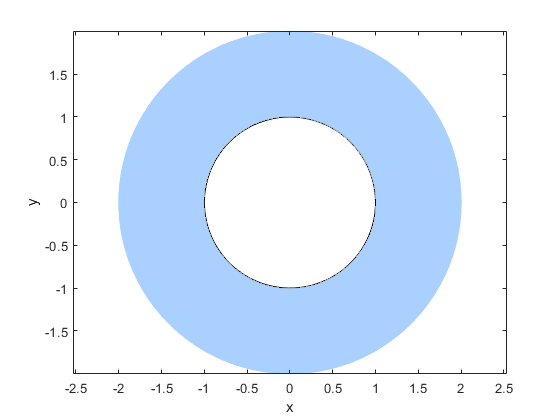
\includegraphics[width=3.5in,height=2.0in]{3_1_8.png}
  \end{center}
  where blue represents points in the domain of $f$ and white those that are not (note: entire border  of the outer circle is included, but not that of the inner circle!). 
  \\
  \\
  \item[{\small\bf 9}.] $f(x,y,z)=x/(yz)$.
  \\
  \\
  {\sc Solution}: As above, we begin by finding the "problem points". Here, we now work with $\mathbb{R}^3$ instead of $\mathbb{R}^2$, so all our inequalities will be in space. The only issue is when $yz=0 \ \Leftrightarrow \ y=0,z=0$ because $1/(yz)$ is not defined there. So the domain of $f$ is
  $$D=\{(x,y,z)\in \mathbb{R}^3 \ | \  y \neq 0, z\neq 0 \}$$ 
  a sketch is
  \begin{center}
  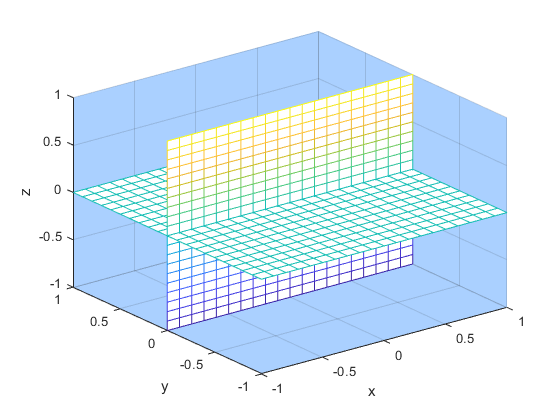
\includegraphics[width=3.5in,height=2.0in]{3_1_9.png}
  \end{center}
  where blue represents points in the domain of $f$ and the white grid planes are not included. 
  \\
  \\
  \item[{\small\bf 10}.] $f(x,y,z)=x/(x-y^2-z^2)$.
  \\
  \\
  {\sc Solution}: As above, we begin by finding the "problem points". The only issue is when $x-y^2-z^2=0 \ \Leftrightarrow \ x=y^2+z^2$ because $1/(x-y^2-z^2)$ is not defined there. So the domain of $f$ is
  $$D=\{(x,y,z)\in \mathbb{R}^3 \ | \  x\neq y^2+z^2 \}$$ 
  a sketch is
  \begin{center}
  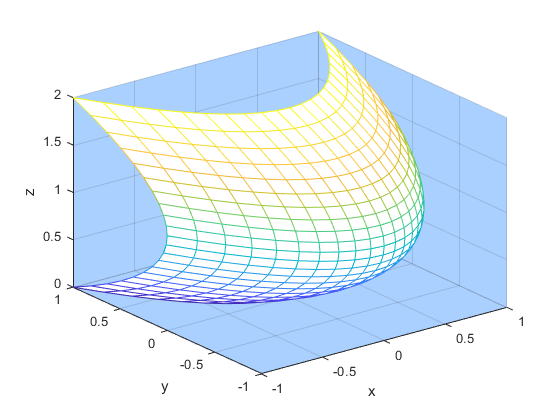
\includegraphics[width=3.5in,height=2.0in]{3_1_10.png}
  \end{center}
  where blue represents points in the domain of $f$ and the white grid paraboloid is not included. 
  \\
  \\
  \item[{\small\bf 11}.] $f(x,y,z)=\ln(1-z+x^2+y^2)$.
  \\
  \\
  {\sc Solution}: As above, we begin by finding the "problem points". The only issue is when $1-z+x^2+y^2 \leq 0 \ \Leftrightarrow \ x^2+y^2 \leq z -1$ because $\ln(1-z+x^2+y^2)$ is not defined there. So the domain of $f$ is
  $$D=\{(x,y,z)\in \mathbb{R}^3 \ | \  z -1 < x^2+y^2\}$$ 
  a sketch is
  \begin{center}
  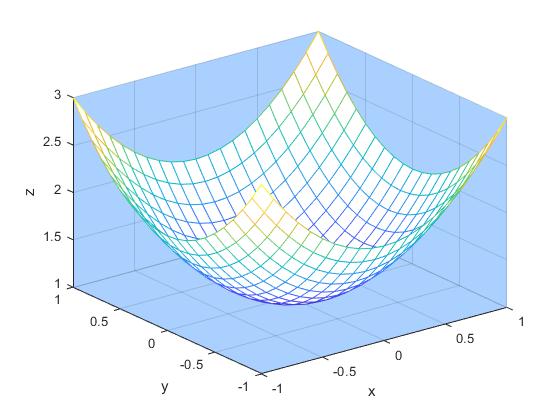
\includegraphics[width=3.5in,height=2.0in]{3_1_11.png}
  \end{center}
  where blue represents points in the domain of $f$. The region above and including the paraboloid is not included. 
  \\
  \\
  \item[{\small\bf 12}.] $f(x,y,z)=\sqrt{x^2-y^2-z^2}+\ln(1-x^2-y^2-z^2)$.
  \\
  \\
  {\sc Solution}: As above, we begin by finding the "problem points". There are two simple functions, the square root and the logarithm. For the square root, the problem  points are when $x^2-y^2-z^2 < 0 \ \Leftrightarrow \ x^2<y^2+z^2$. For the logarithm, the problem points are when $1-x^2-y^2-z^2 \leq 0 \ \Leftrightarrow \ 1 \leq x^2+y^2+z^2$. So the domain of $f$ is
  $$D=\{(x,y,z)\in \mathbb{R}^3 \ | \  x^2+y^2+z^2<1,  x^2\geq y^2+z^2 \}$$ 
  a sketch is
  \begin{center}
  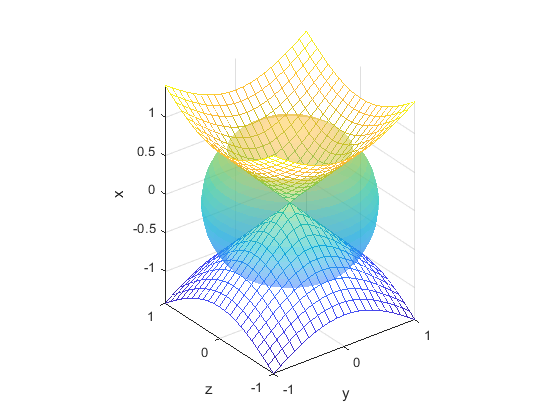
\includegraphics[width=3.5in,height=2.0in]{3_1_12.png}
  \end{center}
  The domain is the region between the double cone and the unit sphere, not including the boundary of the unit sphere.  
  \\
  \\
  \item[{\small\bf 13}.] $f(t,{\bf r})=(t^2-\|{\bf r}\|^2)^{-1}, \ {\bf r}=\la x_1,x_2,...,x_n \ra$.
  \\
  \\
  {\sc Solution}: As above, we begin by finding the "problem points". This is when $t= \pm \|{\bf r}\|$. So the domain of $f$ is
  $$D=\{(t,x_1,...,x_n)\in \mathbb{R}^{n+1} \ | \  t \neq \pm \|{\bf r}\| \}$$ 
There is no good way to sketch this for general $n$.
  \\
  \\
\end{enumerate}

\noindent
{\small {\bf 14}--{\bf 19}}. For each of the following functions, sketch a contour map and use
it to sketch the graph:
\begin{enumerate}
  \item[{\small\bf 14}.] $f(x,y)=x^2+4y^2$;
  \\
  \\
  {\sc Solution}: For each of these problems, we let $f(x,y)=k$, where $k$ is in the range of $f$. This is simply a level set of $f$, and a contour plot is a collection of level sets. To sketch the graph, we interpret $k$ as $z$; thus, take the contour plot, and "raise" or "lower" a each contour by its $k$. Here, we have $x^2+4y^2=k$, where $k$ is a nonnegative real number (since the sum of two positive numbers is always positive). This is clearly an ellipse, given by $x^2/k+y^2/(k/4)=1$ for nonzero $k$; when $k=0$, the contour is simply the origin. Thus we have
  \\
  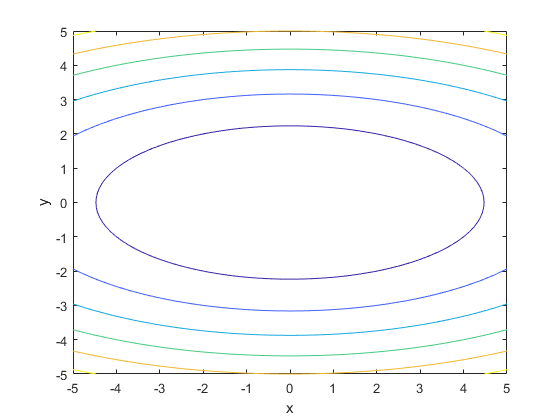
\includegraphics[width=3.5in,height=2.0in]{3_1_14_1.png}
  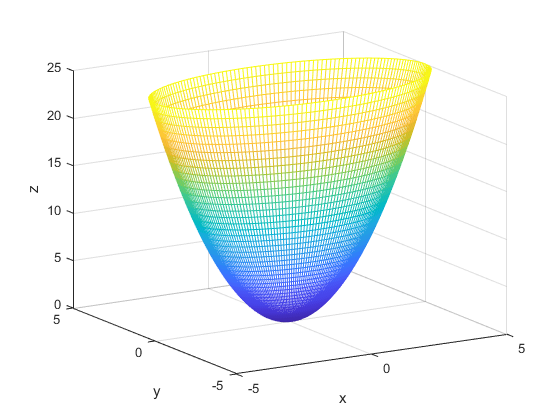
\includegraphics[width=3.5in,height=2.0in]{3_1_14_2.png}
  the contours closer to blue correspond to lower $k$ values and those in yellow correspond to greater $k$ values. A sketch of the graph is produced to the right. This is an elliptic paraboloid.
  \\
  \\
  \item[{\small\bf 15}.] $f(x,y)=xy$;
  \\
  \\
  {\sc Solution}: As above, we begin by forming the contour plot using multiple level sets. Here, we have $xy=k$, where $k$ is a real number. This is a hyperbola for nonzero $k$ given by $y=k/x$. For positive $k$, the level sets are hyperbolas in the 1st and 3rd quadrant; for negative $k$, in the 2nd and 4th. When $k=0$, the contour is $xy=0 \ \Leftrightarrow \ x=0,y=0$. Thus we have
  \\
  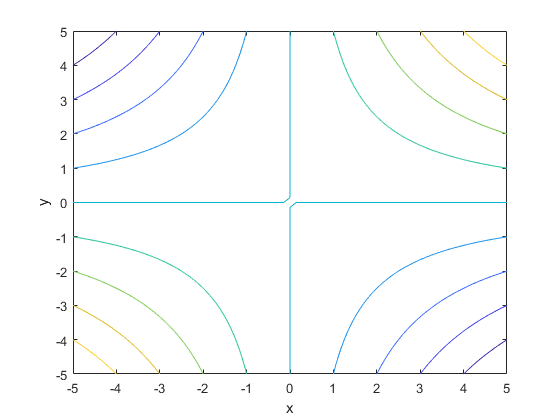
\includegraphics[width=3.5in,height=2.0in]{3_1_15_1.png}
  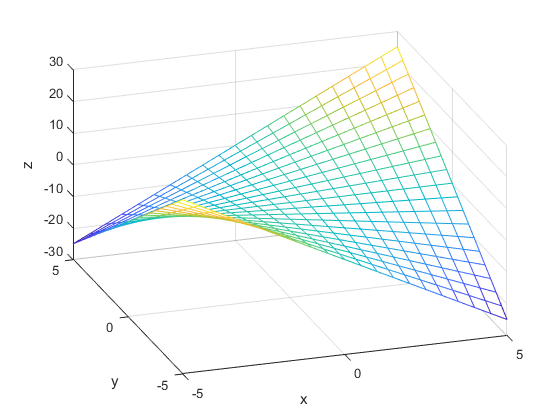
\includegraphics[width=3.5in,height=2.0in]{3_1_15_2.png}
  the contours closer to blue correspond to lower $k$ values (teal is $k=0$) and those in yellow correspond to greater $k$ values. A sketch of the graph is produced to the right. Note that this is a saddle rotated by 45 degrees, aligned along $y=x$. 
  \\
  \\
  \item[{\small\bf 16}.] $f(x,y)=x^2-y^2$;
  \\
  \\
  {\sc Solution}: As above, we begin by forming the contour plot using multiple level sets. Here, we have $x^2-y^2=k$, where $k$ is a real number. This is a hyperbola for nonzero $k$ given by $y=\pm \sqrt{x^2-k}$. For positive $k$, the level sets are hyperbolas in the opening along the $x$-axis; for negative $k$, along the $y$-axis. When $k=0$, the contour is $x^2-y^2=0 \ \Leftrightarrow \ y=\pm x$. Thus we have
  \\
  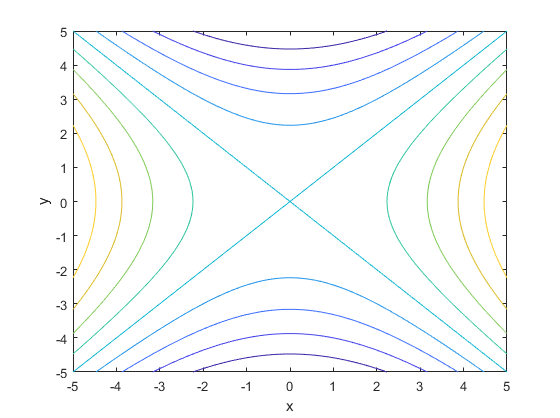
\includegraphics[width=3.5in,height=2.0in]{3_1_16_1.png}
  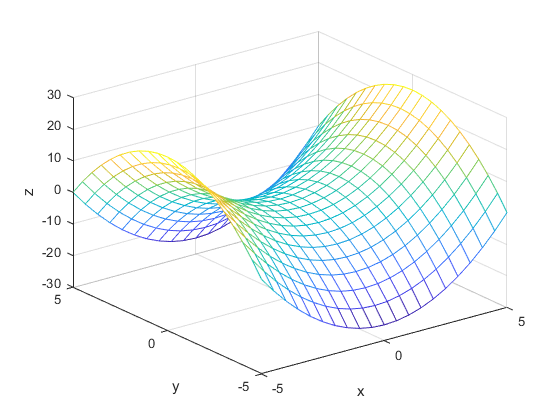
\includegraphics[width=3.5in,height=2.0in]{3_1_16_2.png}
  the contours closer to blue correspond to lower $k$ values (teal is $k=0$) and those in yellow correspond to greater $k$ values. A sketch of the graph is produced to the right. Note that this is a saddle in its canonical form. 
  \\
  \\
  \item[{\small\bf 17}.] $f(x,y)=\sqrt{x^2+9y^2}$;
  \\
  \\
  {\sc Solution}: As above, we begin by forming the contour plot using multiple level sets. Here, we have $\sqrt{x^2+9y^2}=k$, where $k$ is a nonnegative real number. This is an ellipse given by $x^2/k^2+y^2/(k^2/9)=1$. When $k=0$, the contour is $\sqrt{x^2+9y^2}=0$ which consists of only the origin. Thus we have
  \\
  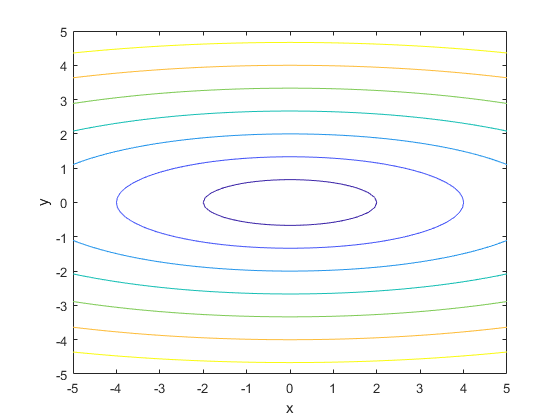
\includegraphics[width=3.5in,height=2.0in]{3_1_17_1.png}
  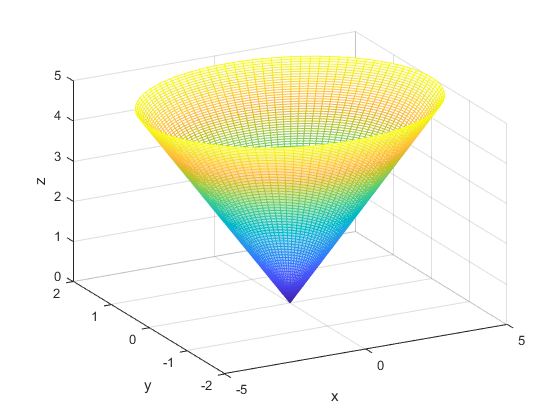
\includegraphics[width=3.5in,height=2.0in]{3_1_17_2.png}
  the contours closer to blue correspond to lower $k$ values and those in yellow correspond to greater $k$ values. A sketch of the graph is produced to the right. This is a cone. 
  \\
  \\
  \item[{\small\bf 18}.] $f(x,y)=\sin x$;
  \\
  \\
  {\sc Solution}: As above, we begin by forming the contour plot using multiple level sets. Here, we have $\sin x=k$, where $k$ satisfies $-1 \leq k \leq 1$. The contour is a collection of parallel lines given by $x=\arcsin k$, repeating as necessary. Note that there is no dependent on $y$, so the surface will look the same for any $y$; you can imagine the surface as being formed by taking the planar curve $\sin x$ and placing a copy for each $y$. Thus we have
  \\
  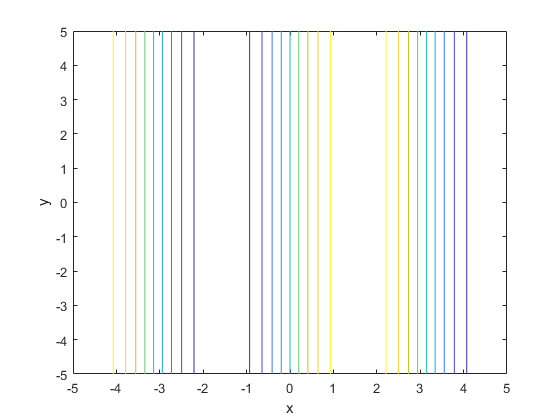
\includegraphics[width=3.5in,height=2.0in]{3_1_18_1.png}
  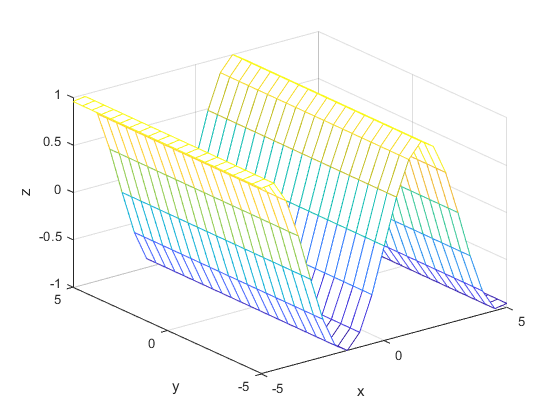
\includegraphics[width=3.5in,height=2.0in]{3_1_18_2.png}
  the contours closer to blue correspond to lower $k$ values and those in yellow correspond to greater $k$ values. A sketch of the graph is produced to the right.
  \\
  \\
  \item[{\small\bf 19}.] $f(x,y)=y^2+(1-\cos x)$.
  \\
  \\
  {\sc Solution}: As above, we begin by forming the contour plot using multiple level sets. Here, we have $y^2+(1-\cos x)=k$, where $k$ is a real number.  Thus we have
  \\
  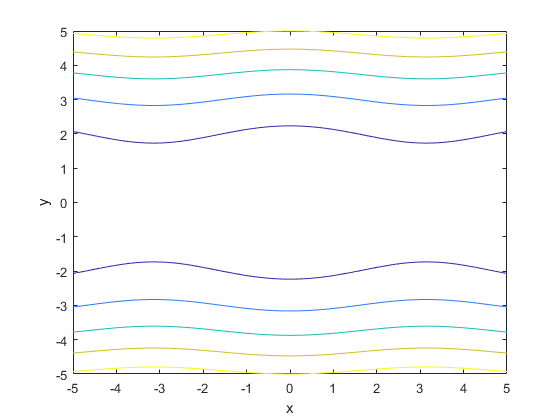
\includegraphics[width=3.5in,height=2.0in]{3_1_19_1.png}
  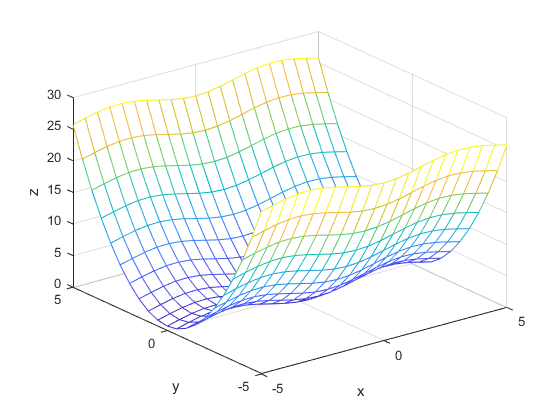
\includegraphics[width=3.5in,height=2.0in]{3_1_19_2.png}
  the contours closer to blue correspond to lower $k$ values and those in yellow correspond to greater $k$ values. A sketch of the graph is produced to the right.
\end{enumerate}

\noindent
{\small {\bf 20}--{\bf 25}}. Describe and sketch the level sets of each of the following functions:
\begin{enumerate}
  \item[{\small\bf 20}.] $f(x,y,z)=x+2y+3z$;
  \\
  \\
  {\sc Solution}: The level sets for each of these problem will be level surfaces. Thus we must describe and sketch the surfaces. To do this, we set $f(x,y,z)=k$ for $k$ in the range of $f$. Here we have $x+2y+3z=k$ for real $k$. These are parallel planes with normal vector ${\bf n}=\la 1,2,3 \ra$. The level sets for $k=-10,0,10$ are produced below:
  \begin{center}
  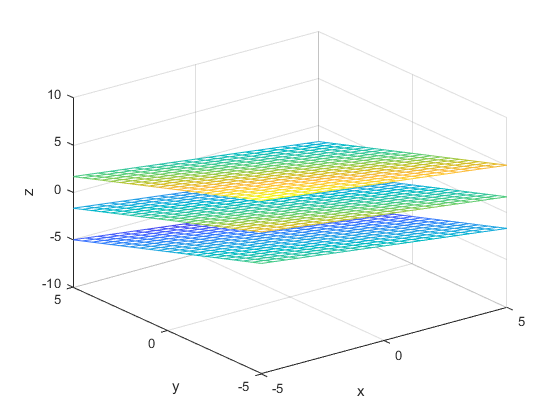
\includegraphics[width=3.5in,height=2.0in]{3_1_20.png}
  \end{center}
  \item[{\small\bf 21}.] $f(x,y,z)=x^2+4y^2+9z^2$;
  \\
  \\
  {\sc Solution}: As above, we set $f(x,y,z)=k$ for $k$ in the range of $f$. Here we have $x^2+4y^2+9z^2=k^2$ for nonnegative real $k$. Using $k^2$ rather than $k$ is merely an aesthetic choice. When $k=0$, we have $x^2+4y^2+9z^2=0$, the only solution of which is the origin (since the sum of three nonnegative numbers, not all zero, is nonzero). For positive $k$, we have $(x/k)^2+(y/(k/2))^2+(z/(k/3))^2=1$. This is an ellipsoid with axes along the $x$, $y$, and $z$ axis of length $2k$, $k$, and $2/3k$. The level sets for $k=0,1,2$ are produced below:
  \begin{center}
  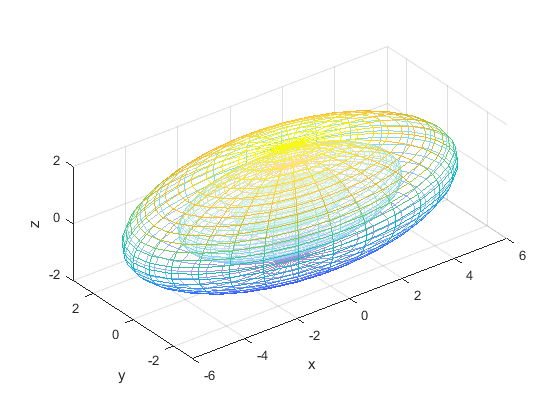
\includegraphics[width=3.5in,height=2.0in]{3_1_21.png}
  \end{center}
  \item[{\small\bf 22}.] $f(x,y,z)=z+x^2+y^2$;
  \\
  \\
  {\sc Solution}: As above, we set $f(x,y,z)=k$ for $k$ in the range of $f$. Here we have $z+x^2+y^2=k$ for real $k$. Note that this can be rearranged as $(z-k)=-(x^2+y^2)$; clearly, an elliptic paraboloid shifted concave down shifted $k$ units in the positive $z$ direction. The level sets for $k=0,1,2$ are produced below:
  \begin{center}
  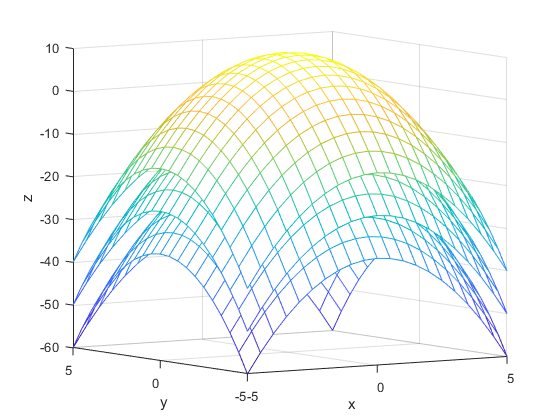
\includegraphics[width=3.5in,height=2.0in]{3_1_22.png}
  \end{center}
  \item[{\small\bf 23}.] $f(x,y,z)=x^2+y^2-z^2$;
  \\
  \\
  {\sc Solution}: As above, we set $f(x,y,z)=k$ for $k$ in the range of $f$. Here we have $x^2+y^2-z^2=k$ for real $k$. In the case when $k=0$, we have $z^2=x^2+y^2$, a cone. When $k$ is nonzero, we have $x^2/k+y^2/k-z^2/k=1$. The surface depends on the sign of $k$; if $k$ is positive, this is a hyperboloid of one sheets otherwise it is a hyperholoid of two sheets. The level sets for $k=-1/2,0,1/2$ (from inner to outer) are produced below:
  \begin{center}
  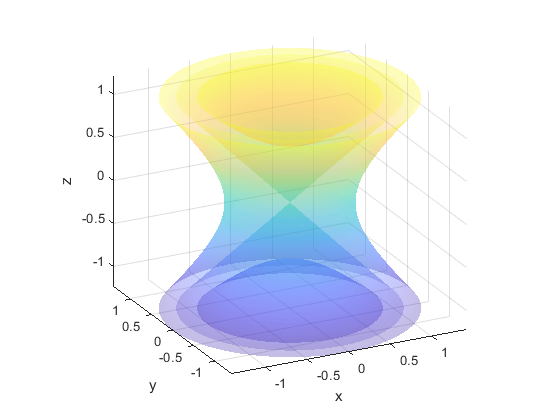
\includegraphics[width=3.5in,height=2.0in]{3_1_23.png}
  \end{center}
  \item[{\small\bf 24}.] $f(x,y,z)=\ln(x^2+y^2-z^2)$;
  \\
  \\
  {\sc Solution}: As above, we set $f(x,y,z)=k$ for $k$ in the range of $f$. Here we have $\ln(x^2+y^2-z^2)=k$ for real $k$. However, we can manipulate this to $x^2+y^2-z^2=e^k=K$ for some positive $K$ (since $e^k$ is never negative). Thus we are in a special case of Exercise {\bf 23} where we only have hyperboloids of one sheet. The level sets for $K=e^{-2},(e^2+e^{-2})/2,e^2$ (from inner to outer) are produced below:
  \begin{center}
  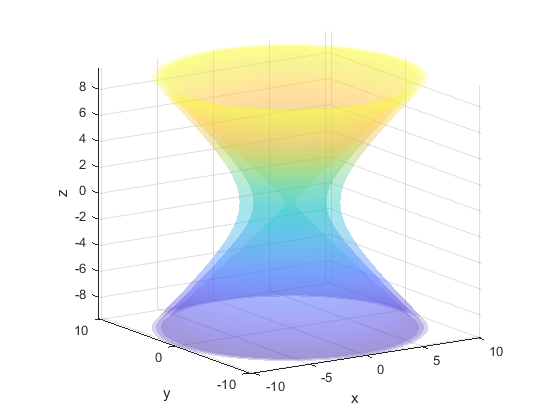
\includegraphics[width=3.5in,height=2.0in]{3_1_24.png}
  \end{center}
  \item[{\small\bf 25}.] $f(x,y,z)=\ln(z^2-x^2-y^2)$.
  \\
  \\
  {\sc Solution}: As above, we set $f(x,y,z)=k$ for $k$ in the range of $f$. Here we have $\ln(z^2-x^2-y^2)=k$ for real $k$. However, we can manipulate this to $z^2-x^2-y^2=e^k=K$ for some positive $K$ (since $e^k$ is never negative). Thus we are in a special case of Exercise {\bf 23} where we only have hyperboloids of two sheets. The level sets for $K=e^{-2},(e^2+e^{-2})/2,e^2$ (from outer to inner) are produced below:
  \begin{center}
  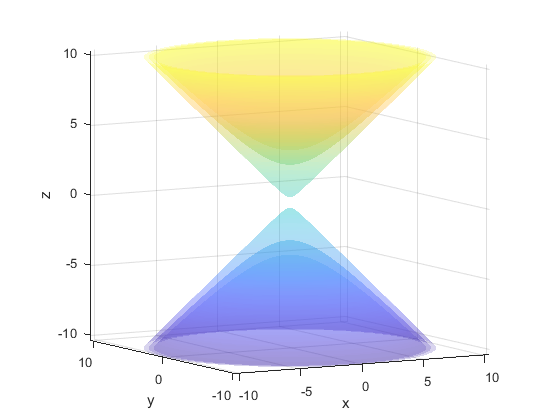
\includegraphics[width=3.5in,height=2.0in]{3_1_25.png}
  \end{center}
\end{enumerate}

\noindent
{\small {\bf 26}--{\bf 32}}. Sketch the level sets of each of the following functions. Here
$\operatorname{min}(a, b)$ and $\operatorname{max}(a, b)$ denote the smallest number and the largest number
of $a$ and $b$, respectively, and $\operatorname{min}(a, a)=\operatorname{max}(a, a)=a$.
\begin{enumerate}
  \item[{\small\bf 26}.] $f(x,y)=|x|+y$;
  \\
  \\
  {\sc Solution}: Here, the level sets are given by $|x|+y=k \ \Leftrightarrow \ y=k-|x|$ for real $k$. This is simply a vertical translation of $y=-|x|$ by $k$ units. The level sets are shown as a contour plot below:
  \begin{center}
  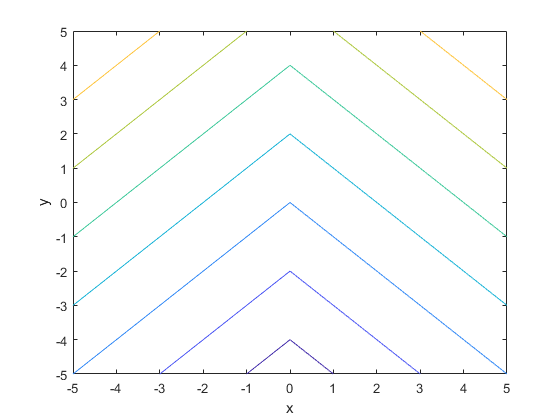
\includegraphics[width=3.5in,height=2.0in]{3_1_26.png}
  \end{center}
  \item[{\small\bf 27}.] $f(x,y)=|x|+|y|-|x+y|$;
  \\
  \\
  {\sc Solution}: Here, the level sets are given by $|x|+|y|-|x+y|=k$ for nonnegative $k$. $k$ must be nonnegative because, due to the triangle inequality, we have
  $$|x+y|\leq |x|+|y| \ \Leftrightarrow \ -|x+y|\geq-|x|-|y| \ \Leftrightarrow \ |x|+|y|-|x+y| \geq 0$$
   Suppose $k=0$. Then $|x|+|y|-|x+y|=0$. Let $y=0$, then $|x|-|x|=0$, which is true for all $x$. A similar argument holds for $x=0$. Thus the lines $x=0,y=0$ are the level set for $k=0$. Next, let $k>0$. It follows that $x=k/2,y=-k/2$ is a solution, since
   $$|k/2|+|-k/2|-|k/2-k/2|=k/2+k/2-0=k$$
   The same is true for $x=-k/2,y=k/2$. Suppose $x=k/2$. Then 
   $$|k/2|+|y|-|y+k/2|=k \ \Leftrightarrow \ |y|-|y+k/2|=k/2$$
   Suppose now that $y> -k/2$. Then $y+k/2>0$, and so $|y+k/2|=y+k/2$. However, $y+k/2>y$, so $|y|-|y+k/2|<0$. But $k$ is positive, so this cannot be. Clearly, the issue is with the equality $|y+k/2|=y+k/2$. Suppose now that $y \leq -k/2$. Then $|y+k/2|=-(y+k/2)$. We still have that $y+k/2>y$, and so $-y>-(y+k/2)$. Since $-y=|y|$ (both quantities are positive, $y$ is negative), we have $|y|-|y+k/2|>0$. In this case, we actually have direct equality. Thus the line $x=k/2$ for $y\leq -k/2$ is part of the contour. Additionally, we have $y=-k/2$ for $x \geq k/2$, $x=-k/2$ for $y \geq k/2$, and $y=k/2$ for $x \leq -k/2$. The level sets are shown as a contour plot below:
  \begin{center}
  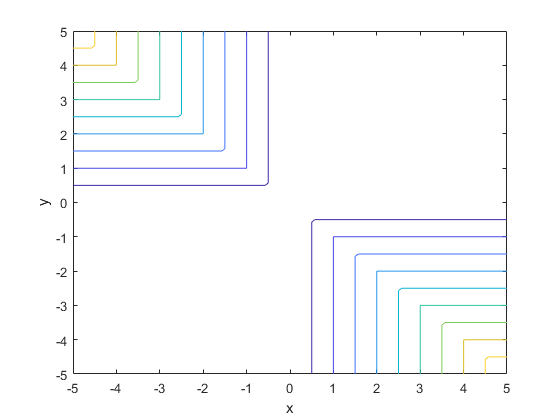
\includegraphics[width=3.5in,height=2.0in]{3_1_27.png}
  \end{center}
  \item[{\small\bf 28}.] $f(x,y)=\operatorname{min}(x, y)$;
  \\
  \\
  {\sc Solution}: Here, the level sets are given by $\operatorname{min}(x, y)=k$ for real $k$. First, recall that $\operatorname{min}(x, x)=x$, so clearly $(k,k)$ is a solution. Fix $x=k$. Then for any $y \geq k$, $\operatorname{min}(x, y)=x=k$. Next, fix $y=k$. Then for any $x \geq k$, $\operatorname{min}(x, y)=y=k$. So the level set consists of the two lines $x=k$ for $y \geq k$ and $y=k$ for $x \geq k$. 
   The level sets are shown as a contour plot below:
  \begin{center}
  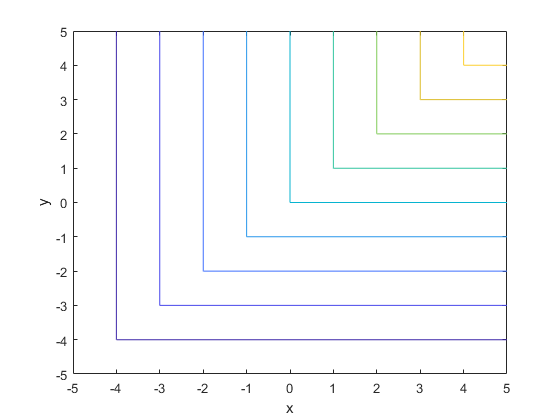
\includegraphics[width=3.5in,height=2.0in]{3_1_28.png}
  \end{center}
  \item[{\small\bf 29}.] $f(x,y)=\operatorname{max}(|x|, |y|)$;
    \\
  \\
  {\sc Solution}: Here, the level sets are given by $\operatorname{max}(|x|, |y|)=k$ for real $k$. First, recall that $\operatorname{max}(x, x)=x$, so clearly $(k,k)$ and $(-k,-k)$ are solutions. Fix $x=\pm k$. Then for any $-k \leq y \leq k$, $\operatorname{max}(|x|, |y|)=|x|=k$. Next, fix $y=\pm k$. Then for any $-k \leq x \leq k$, $\operatorname{max}(|x|, |y|)=y=k$. So the level set consists of the four lines $x=\pm$ for $y \geq k$ and $y=\pm k$ for $x \geq k$. Incidentally, these make squares of side length $2k$.
   The level sets are shown as a contour plot below:
  \begin{center}
  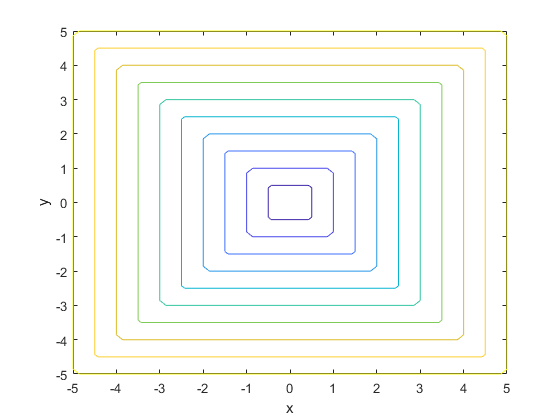
\includegraphics[width=3.5in,height=2.0in]{3_1_29.png}
  \end{center}
  \item[{\small\bf 30}.] $f(x,y)=\operatorname{sign}(\sin x \sin y)$; here $\operatorname{sign}(a)$ is the sign function, it
has the values $1$ and $−1$ for positive and negative $a$, respectively.
  \\
  \\
  {\sc Solution}: Here, the level sets are given by $\operatorname{sign}(\sin x \sin y)=k$ for $k=-1,0,1$. Recall that $\sin(x)=0$ for $x=n\pi$ where $n$ is an integer. Thus $\operatorname{sign}(\sin x \sin y)$ partitions $\mathbb{R}^2$ with grid lines at $x=n\pi$ and $y=n\pi$. Focus on the plot with $0\leq x \leq 2\pi$ and $0\leq y \leq 2\pi$. This region is subdivided into four squares (by the lines $x=\pi$ and $y=\pi$). In the lower left ($0< x < \pi$ and $0< y < \pi$), $\sin x$ and $\sin y$ are both positive, so $\operatorname{sign}(\sin x \sin y)=1$. Next, in the lower right ($\pi< x < 2\pi$ and $0< y < \pi$) square, $\sin x$ is negative whereas $\sin y$ is positive, so $\operatorname{sign}(\sin x \sin y)=-1$. In the upper left ($0< x < \pi$ and $\pi < y < 2\pi$) square, $\sin x$ is positive whereas $\sin y$ is negative, so $\operatorname{sign}(\sin x \sin y)=-1$. Finally, in the upper right ($\pi < x < 2\pi$ and $\pi < y < 2\pi$) square, $\sin y$ is negative and $\sin y$ is negative, so $\operatorname{sign}(\sin x \sin y)=1$. Due to the periodic nature of $\sin$, this plot may be tessellated to cover all of $\mathbb{R}^2$. 
   The level sets are shown as a contour plot below:
  \begin{center}
  \includegraphics[width=3.5in,height=2.0in]{3_1_30.png}
  \end{center}
  Unfortunately, MATLAB would not color the space appropriately. All white spaces should either be shaded yellow/blue, depending on the border of the square. Teal corresponds to $0$.
  \\
  \\
  \item[{\small\bf 31}.] $f(x,y)=(x+y)^2+z^2$;
  \\
  \\
  {\sc Solution}: Here, the level sets are given by $(x+y)^2+z^2=k$ for nonnegative $k$. Let $x=x'\cos(\phi)-y'\sin(\phi)$ and $y=y'\cos(\phi)+x'\sin(\phi)$ [Recall Chapter 1]. Then 
  $$x+y=x'(\cos(\phi)+\sin(\phi))+y'(\cos(\phi)-\sin(\phi))=\sqrt{2}x'\cos(\phi-\frac{\pi}{4})-\sqrt{2}y'\sin(\phi-\frac{\pi}{4}),$$
  so we have that
  $$(x+y)^2=2(x'^2\cos(\phi-\frac{\pi}{4})^2-2x'y'\cos(\phi-\frac{\pi}{4})\sin(\phi-\frac{\pi}{4})+y'^2\sin(\phi-\frac{\pi}{4})^2)$$
  We wish to remove the mixed term, so let $\phi = \pi/4$. Then the level sets are given by
  $$2x'^2+z^2=k$$
  which are evidently elliptic cylinders that have been rotated by $\pi/4$ (aligned along $y=-x$, because there are no solutions there!). 
   The level sets are shown with the surfaces ($k=1,4,9$, from inner to outer) below:
  \begin{center}
  \includegraphics[width=3.5in,height=2.0in]{3_1_31.png}
  \end{center}
  \item[{\small\bf 32}.] $f(x,y)=\arctan(2ay/(x^2+y^2-a^2)), \ a>0$.
  \\
  \\
  {\sc Solution}: Here, the level sets are given by $\arctan(2ay/(x^2+y^2-a^2))=k$ for real $k$ satisfying $-\pi/2<k<\pi/2$ (the range follows from the natural restriction of arctangent). This can be rearranged to give $2ay=\tan(k)(x^2+y^2-a^2)$. After completing the square, one yields
  $$x^2+(y-a/\tan(k))^2=a^2+(a/\tan(k))^2$$
  Evidently these are circles with radius $\sqrt{a^2+(a/\tan(k))^2}$ and center $(0,a/\tan(k))$. \
   The level sets are shown with the surfaces below:
  \begin{center}
  \includegraphics[width=3.5in,height=2.0in]{3_1_32.png}
  \end{center}
\end{enumerate}

\noindent
{\small {\bf 33}--{\bf 36}}. Explain how the graph $z = g(x, y)$ can be obtained from the graph
of $f(x, y)$ if
\begin{enumerate}
  \item[{\small\bf 33}.] $g(x,y)=k+f(x,y)$, where $k$ is a constant;
  \\
  \\
  {\sc Solution}: Recall that $z-k$ for a constant $k$ simply describes a shift by $k$ units in the positive $z$ direction. So $g(x,y)=k+f(x,y)$ is a translation of $f(x,y)$ by $k$ units.
  \\
  \item[{\small\bf 34}.] $g(x,y)=mf(x,y)$, where $m$ is a nonzero constant;
  \\
  \\
  {\sc Solution}: First, suppose $m>0$. In this case $g(x,y)=mf(x,y)$ is obtained where $f(x,y)$ is shrunk ($0<m<1$) or stretched ($1<m$). Next, suppose $m<0$. Then $g(x,y)=mf(x,y)$ is obtained by first reflecting $f$ over the $xy$ plane, then stretching/shrinking $f$.
  \\
  \item[{\small\bf 35}.] $g(x,y)=f(x-a,y-b)$, where $a$ and $b$ are constants;
  \\
  \\
  {\sc Solution}: As with Exercise {\bf 33}, $g(x,y)=f(x-a,y-b)$ is obtained by translating $f$ by $a$ units along the $x$ axis and $b$ units along the $y$ axis.
  \\
  \item[{\small\bf 36}.] $g(x,y)=f(px,qy)$, where $p$ and $q$ are nonzero constants.
  \\
  \\
  {\sc Solution}: As with Exercise {\bf 34}, the same shrinking/stretching effect occurs along each axis depending on the sign of $p,q$ and whether $|p|,|q|>1$.
  \\
\end{enumerate}

\noindent
{\small {\bf 37}--{\bf 39}}. Given a function $f(x, y)$, sketch the graphs of the function $g(x, y)$
defined in Exercises {\bf 33}-{\bf 36}. Analyze carefully various cases for values of the
constants (for example, $m > 0$, $m < 0$, $p > 1$, $0 < p < 1$, and $p = -1$, etc.)
\begin{enumerate}
  \item[{\small\bf 37}.] $f(x,y)=x^2+y^2$;
  \\
  \\
  {\sc Solution}: Let $f(x,y)=x^2+y^2$. Note that $f(y,x)=f(x,y)$, so there is no reason to investigate changes in $q$. Further observe that $f$ is even with respect to both $x$ and $y$, so $f(px,qy)=f(-px,-qy)$, and thus these cases will not be investigated. The plot to the left includes $z=f(x,y)$ and $z=\pm 4f(x,y)$. The plot to the right includes $z=f(2x,y)$, $z=f(x,y)$, and $z=f(x/2,y)$ (from inner to outer).
  \\
  \includegraphics[width=3.5in,height=2.0in]{3_1_37_1.png}
  \includegraphics[width=3.5in,height=2.0in]{3_1_37_2.png}
  \item[{\small\bf 38}.] $f(x,y)=xy$;
  \\
  \\
  {\sc Solution}: Let $f(x,y)=xy$. Note that $f(y,x)=f(x,y)$, so there is no reason to investigate changes in $q$. Further observe that $f(px,y)=pf(x,y)$, thus these cases will not be investigated. The plot to the left includes $z=f(x,y)$ and $z=2f(x,y)=f(2x,y)$. The plot to the right includes $z=f(x,y)$ and $z=-2f(x,y)=f(-2x,y)$
  \\
  \includegraphics[width=3.5in,height=2.0in]{3_1_38_1.png}
  \includegraphics[width=3.5in,height=2.0in]{3_1_38_2.png}
  \item[{\small\bf 39}.] $f(x,y)=(a^2-x^2-y^2)^2$.
  \\
  \\
  {\sc Solution}: Let $f(x,y)=(a^2-x^2-y^2)^2$. Note that $f(y,x)=f(x,y)$, so there is no reason to investigate changes in $q$. Further observe that $f$ is even with respect to both $x$ and $y$, so $f(px,qy)=f(-px,-qy)$, and thus these cases will not be investigated. The plot to the left includes $z=f(x,y)$ and $z=\pm 2f(x,y)$. The plot to the right (note: which is scaled differently) includes $z=f(x,y)$, $z=f(2x,y)$, and $z=f(x/2,y)$
  \\
  \includegraphics[width=3.5in,height=2.0in]{3_1_39_1.png}
  \includegraphics[width=3.5in,height=2.0in]{3_1_39_2.png}
\end{enumerate}

\noindent
{\small\bf 40}. Find $f(u)$ if $f(x/y) = \sqrt{x^2+y^2}/x, \ x>0$.
\\
\\
{\sc Solution}: The goal is to express all instances of $x$ and $y$ in $f(x/y)$ in terms of $x/y$ or $y/x$. Then we may substitute $u=x/y$ and $1/u=y/x$. This is just algebra.
$$f(\frac{x}{y})=\frac{\sqrt{x^2+y^2}}{x}=\sqrt{1+\frac{y^2}{x^2}}=\sqrt{1+(\frac{y}{x})^2}$$
so with $u=x/y$, $f(u)=\sqrt{1+1/u^2}=\sqrt{u^2+1}/u$.
\\
\\
{\small\bf 41}. Find $f(x,y)$ if $f(x+y,y/x)=y^2-x^2$
\\
\\
{\sc Solution}: I will solve this by making the substitutions $u=x+y$ and $v=y/x$. Note that we can solve for $x,y$ as follows. We have that $y=vx$. Substitution of this into the former equation gives $u=x+vx=(1+v)x$, so $x=u/(1+v)$. Substituting this back gives $y=v(u/(1+v))=uv/(1+v)$. Then we have
$$f(u,v)=(\frac{uv}{1+v})^2-(\frac{u}{1+v})^2=\frac{u^2}{(1+v)^2}(v^2-1)=\frac{u^2(v-1)}{1+v}$$
A simple cosmetic change provides $f(x,y)$ as $f(x,y)=x^2(y-1)/(y+1)$.
\\
\\
{\sc Alternative Solution}: One can also simply perform the following algebraic manipulations
$$f(x+y,y/x)=(y+x)(y-x)=(y+x)^2\frac{y-x}{y+x}=(x+y)^2\frac{y/x-1}{y/x+1},$$
but I find this to be far less intuitive.
\\
\\
{\small\bf 42}. Let $z=\sqrt{y}+f(\sqrt{x}-1)$. Find the functions $z$ and $f$ if $z=x$ when $y=1$.
\\
\\
{\sc Solution}: Suppose $z=x$ when $y=1$. Let $y=1$. Then 
$$x=1+f(\sqrt{x}-1) \ \Leftrightarrow \ f(\sqrt{x}-1)=x-1$$
and $f(x)=(x+1)^2-1$. Direct substitution verifies this:
$$f(\sqrt{x}-1)=(\sqrt{x}-1+1)^2-1=\sqrt{x}^2-1=x-1$$ 
Also, $z=\sqrt{y}+f(\sqrt{x}-1)=\sqrt{y}+x-1$. 
\\
\\
{\small\bf 43}. Graph the function $F(t) = f(\cos t,\sin t)$ where $f(x, y) = 1$ if $y \geq x$ and
$f(x, y) = 0$ if $y < x$. Give a geometrical interpretation of the graph of $F$ as
an intersection of two surfaces.
\\
\\
{\sc Solution}: First let us determine what the surface $z=f(x,y)$ looks like. Consider the plane $y=x$. Everything "above" this plane (with $y \geq x$) will be at $z=1$, and everything below will be at $z=0$. Note that $\cos t = \sin t$ for $t=\pi/4+n\pi$ ($n$ integer). On the interval $[0,\pi/4)$, $\cos t > \sin t \ \Leftrightarrow \ x> y$, and so $F(t)=0$. On the interval $[\pi/4,5\pi/4]$, $\sin t \geq \cos t \ \Leftrightarrow \ y \geq x$ and $F(t)=1$. On the interval $(5\pi/4,2\pi]$, $\cos t > \sin t \ \Leftrightarrow \ x> y$, and so $F(t)=0$. Thus $F(t)$ is $1$ if $t$ is in the interval $[\pi/4+2n\pi, 5\pi/4+2n\pi]$ and $0$ if $t$ is in the interval $(5\pi/4+2n\pi, 9\pi/4+2n\pi)$. $F$ is the intersection of the surface $z=f(x,y)$ and the cylinder $x^2+y^2=1$. 
\\
\\
\noindent
{\small {\bf 44}--{\bf 47}}. Let $f(u)$ be a continuous function for all real $u$. Investigate the relation between the shape of the graph of $f$ and the shape of the following
surfaces:
\begin{enumerate}
  \item[{\small\bf 44}.] $z=f(y-ax)$;
  \\
  \\
  {\sc Solution}: Let $f$ be a continuous function. Fix a real $a$. Then $y-ax=d$ represents a particular plane for every $d$. Since $d$ is a constant, if $y-ax=d$, then $f(y-ax)=f(d)$, a constant. Thus $f(y-ax)$ attains a constant value throughout the plane $y-ax=d$. The effect of this is the following: Consider any plane perpendicular to $y=ax$. Then a "copy" of $f(u)$ will be in this plane. Since this is true for every perpendicular plane, a cylinder is formed. The effect of $a$ can be found by referring to Exercise {\bf 36}.
  \\
  \item[{\small\bf 45}.] $z=f(\sqrt{x^2+y^2})$;
  \\
  \\
  {\sc Solution}: Let $f$ be a continuous function. Suppose $\sqrt{x^2+y^2}=r$ for a constant $r$. Then $f(\sqrt{x^2+y^2})=f(r)$, a constant. But we also have $x^2+y^2=r^2$, a circle. So $f$ is constant on circular regions (not a disc!). Imagine taking a circle $x^2+y^2=r^2$ in the $xy$ plane. Then $f(\sqrt{x^2+y^2}$ is produced by lifting this circle $f(r)$ units. The effect is that $z$ is $f$ rotated around the $z$ axis. However, it is only the surface with $z\geq f(0)$, since both $x^2+y^2$ are positive, $r$ can never be negative.
  \\
  \item[{\small\bf 46}.] $z=f(-\sqrt{x^2+y^2})$;
  \\
  \\
  {\sc Solution}: Let $f$ be a continuous function. This is in some sense the opposite of Exercise {\bf 45}. The reason being that only $z \leq f(0)$ are allowed now. More precisely, it is $f(-u)$ rotated about the z axis for $u \geq 0$. So, for functions that are neither even nor odd (e.g., $e^u$), the functions in Exercises {\bf 45} and {\bf 46} will be completely different!
  \\
  \item[{\small\bf 47}.] $z=f(x/y)$;
  \\
  \\
  {\sc Solution}: Let $f$ be a continuous function. Let $x(t)=r \cos t$ for $0 \leq t < 2\pi$ and  $y(t)=r \sin t$ for $0 \leq t < 2\pi$. Then $\la x(t),y(t) \ra$ defines a circle of radius $r$ in the $xy$ plane. Also note that $f(x(t)/y(t))=f(\cot(t))$. So for every circle $x^2+y^2=r^2$, $f$ looks identical.
  \\
\end{enumerate}

\newpage
\section{Limits and Continuity}
\noindent
{\small {\bf 1}--{\bf 5}}. Use Definition {\bf 17.3} of the limit to verify each of the following limits
(i.e., given $\epsilon > 0$, find a neighborhood of the limit point with the properties
specified in the definition):
\begin{enumerate}
  \item[{\small\bf 1}.] $\! \begin{aligned}[t]
 \lim_{{\bf r} \rightarrow {\bf 0}}\frac{x^3-4y^2x+5y^3}{x^2+y^2}=0;  
\end{aligned}$ 
\\
\\
{\sc Solution}: Let $\epsilon >0$. The limit point here is ${\bf 0}$. The distance between ${\bf r}$ and the limit point is 
$$R=\|{\bf r}-{\bf r}_0\|=\|{\bf r}\|=\sqrt{x^2+y^2}$$
From this equality, we immediately receive the following two inequalities:
$$|x| \leq R, \ |y|\leq R$$
where equality is reached when one of $x$ or $y$ (or both) is $0$. 
We will also need the triangle inequality, 
$$|x_1+x_2+...+x_n| \leq |x_1|+|x_2|+...+|x_n|$$
\\
To verify that the limit exists, we need to show that for every $\epsilon >0$, if $\|{\bf r}-{\bf r}_0\| < \delta$ [equivalent to $R<\delta$!] then $|f({\bf r})-0|=|f({\bf r})| < \epsilon$. Thus we need to evaluate the latter quantity in some way, as follows. 
$$|\frac{x^3-4y^2x+5y^3}{x^2+y^2}|\leq \frac{|x|^3+4y^2|x|+5|y|^3}{R^2} \leq \frac{R^3+4R^3+5R^3}{R^2}=10R$$
Note that $x^2+y^2=R^2$. Take close note, in particular, to the sign change of the $4y^2x$ quantity due to the triangle inequality. To get from the second to the third quantity, we employed the two derived inequalities $|x|,|y| \leq R$. 
\\
\\
Now, we require that $|f({\bf r})|<\epsilon$. So if $10R<\epsilon$, then $|f({\bf r})|< \epsilon$. Given $\epsilon>0$, we may choose $10\delta=\epsilon \ \Leftrightarrow \ \delta=\epsilon/10$ to meet the requirements $R<\delta$ and $10R<\epsilon$. However, we may actually choose any $\delta \leq \epsilon/10$; all this does is restrict our choice of $R$ further. 
\\
\item[{\small\bf 2}.] $\! \begin{aligned}[t]
 \lim_{{\bf r} \rightarrow {\bf 0}}\frac{x^3-4y^2x+5y^3}{3x^2+4y^2}=0;
\end{aligned}$ 
\\
\\
{\sc Solution}: Let $\epsilon >0$. The limit point here is ${\bf 0}$. As above, we need to evaluate $|f({\bf r})|$ as follows. 
$$|\frac{x^3-4y^2x+5y^3}{3x^2+4y^2}|\leq \frac{|x|^3+4y^2|x|+5|y|^3}{3x^2+3y^2} \leq \frac{R^3+4R^3+5R^3}{3R^2}=\frac{10R}{3}$$
Note that $3x^2+4y^2 \geq 3x^2+3y^2=3R^2 \ \Leftrightarrow \ 1/(3R^2) \leq 1/(3x^2+4y^2)$. You want all your inequalities to be $\leq$, otherwise you might run into trouble. 
\\
\\
Now, we require that $|f({\bf r})|<\epsilon$. So if $10R/3<\epsilon$, then $|f({\bf r})|< \epsilon$. Given $\epsilon>0$, we may choose $10\delta/3=\epsilon \ \Leftrightarrow \ \delta=3\epsilon/10$ to meet the requirements $R<\delta$ and $10R/3<\epsilon$. However, we may actually choose any $\delta \leq 3\epsilon/10$; all this does is restrict our choice of $R$ further. 
\\
\item[{\small\bf 3}.] $\! \begin{aligned}[t]
 \lim_{{\bf r} \rightarrow {\bf 0}}\frac{x^3-4y^4+5y^3x^2}{3x^2+4y^2}=0; 
\end{aligned}$ 
\\
\\
{\sc Solution}: Let $\epsilon >0$. The limit point here is ${\bf 0}$. As above, we need to evaluate $|f({\bf r})|$ as follows. 
$$|\frac{x^3-4y^4+5y^3x^2}{3x^2+4y^2}|\leq \frac{|x|^3+4y^4+5|y|^3x^2}{3x^2+4y^2} \leq \frac{R^3+4R^4+5R^5}{3R^2} \leq  \frac{R^3+4R^3+5R^3}{3R^2} =\frac{10R}{3}$$
for sufficiently small $R$. This is because for $R<1$, we have $R^5,R^4 < R^3$. So what about when $R>1$? We will get to that later.
\\
\\
Now, we require that $|f({\bf r})|<\epsilon$. So if $10R/3<\epsilon$, then $|f({\bf r})|< \epsilon$. Given $\epsilon>0$, we may choose $10\delta/3=\epsilon \ \Leftrightarrow \ \delta=3\epsilon/10$ to meet the requirements $R<\delta$ and $10R/3<\epsilon$. However, we may actually choose any $\delta \leq 3\epsilon/10$. Remember about the case when $R>1?$. We can avoid this by requiring that $\delta$ is the smallest number between $1$ and $3\epsilon/10$. This is because if $3\epsilon/10$ is greater than $1$, then we will still have that $R<\delta$, and so $R$ may possibly be greater than $1$. However, by restricting $\delta$ in these cases, we can ensure that $R$ is always less than $1$. So, $\delta \leq \delta_1$, where $\delta_1$ is the smallest number between $1$ and $3\epsilon/10$. 
\\
\item[{\small\bf 4}.] $\! \begin{aligned}[t]
 \lim_{{\bf r} \rightarrow {\bf 0}}\frac{x^3-4y^2x+5y^3}{3x^2+4y^2+y^4}=0;
\end{aligned}$ 
\\
\\
{\sc Solution}: Let $\epsilon >0$. The limit point here is ${\bf 0}$. As above, we need to evaluate $|f({\bf r})|$ as follows. 
$$|\frac{x^3-4y^2x+5y^3}{3x^2+4y^2+y^4}|\leq \frac{10R^3}{3R^2+R^4} \leq \frac{10R/3}{(1+R^2/3)} \leq  \frac{10R/3}{1} =\frac{10R}{3}$$
Note that $1+R^2/3 \geq 1 \ \Leftrightarrow 1/(1+R^2/3) \leq 1$ for all $R$, so we do not need to do anything like in Exercise {\bf 3}.
\\
\\
Now, we require that $|f({\bf r})|<\epsilon$. So if $10R/3<\epsilon$, then $|f({\bf r})|< \epsilon$. Given $\epsilon>0$, we may choose $10\delta/3=\epsilon \ \Leftrightarrow \ \delta=3\epsilon/10$ to meet the requirements $R<\delta$ and $10R/3<\epsilon$. However, we may actually choose any $\delta \leq 3\epsilon/10$. 
\\
\item[{\small\bf 5}.] $\! \begin{aligned}[t]
 \lim_{{\bf r} \rightarrow {\bf 0}}\frac{3x^3+4y^4-5y^5}{x^2+y^2+z^2}=0.
\end{aligned}$ 
\\
\\
{\sc Solution}: Let $\epsilon >0$. The limit point here is ${\bf 0}$. As above, we need to evaluate $|f({\bf r})|$ as follows. Note, we have $z$ in this limit; treat it the same as any other variable!
$$|\frac{3x^3+4y^4-5y^5}{x^2+y^2+z^2}|\leq \frac{3R^3+4R^4+5R^5}{R^2} \leq \frac{3R^3+4R^3+5R^3}{R^2} \leq  \frac{12R^3}{R^2} =12R$$
for sufficiently small $R$ (note: we'll have to do something like in Exercise {\bf 3} again!).
\\
\\
Now, we require that $|f({\bf r})|<\epsilon$. So if $12R<\epsilon$, then $|f({\bf r})|< \epsilon$. Given $\epsilon>0$, we may choose $12\delta=\epsilon \ \Leftrightarrow \ \delta=\epsilon/12$ to meet the requirements $R<\delta$ and $12R<\epsilon$. However, we may actually choose any $\delta \leq \delta_1$ where $\delta_1$ is the smallest number between $\epsilon/12$ and $1$. 
\\
\end{enumerate}

\noindent
{\small {\bf 6}--{\bf 8}}. Use the squeeze principle to prove the following limits and find a
neighborhood of the limit point in which the deviation of the function from
the limit value does not exceed a small given number $\epsilon$ (Hint: $|\sin u| \leq |u|$):
\begin{enumerate}
  \item[{\small\bf 6}.] $\! \begin{aligned}[t]
 \lim_{{\bf r} \rightarrow {\bf 0}} y\sin(x/\sqrt{y})=0
\end{aligned}$ 
\\
\\
{\sc Solution}: Recall the squeeze principle is
if there exists a function $h$ of one variable such that
$$|f({\bf r})-c|\leq h(R) \ \rightarrow \ 0 \ \text{as} \ \|{\bf r}-{\bf r}_0\|=R \ \rightarrow 0^+ $$
then the limit as ${\bf r} \rightarrow {\bf r}_0$ of $f({\bf r})$ is $c$. Here, we have
$$R=\|{\bf r}-{\bf 0}\|=\sqrt{x^2+y^2}$$
Using the hint,
$$|y\sin(x/\sqrt{y})-0|\leq |y||\sin(x/\sqrt{y})| \leq |y||x/\sqrt{y}| \leq |x|\sqrt{y} \leq R^{3/2}$$
Evidently, $R^{3/2}$ goes to $0$ as $R$ goes to $0$. Hence the limit exists. To find the neighborhood, simply use the second to last inequality as follows:
$$|y\sin(x/\sqrt{y})|\leq |x|\sqrt{y} \ \Rightarrow \ -|x|\sqrt{y}\leq y\sin(x/\sqrt{y}) \leq |x|\sqrt{y}$$
A delta such that $\delta \leq \epsilon^{2/3}$ may be chosen.
\\
\item[{\small\bf 7}.] $\! \begin{aligned}[t]
\lim_{{\bf r} \rightarrow {\bf 0}}[1-\cos(y/x)]x^2=0
\end{aligned}$ 
\\
\\
{\sc Solution}: As above, we have
$$R=\|{\bf r}-{\bf 0}\|=\sqrt{x^2+y^2}$$
The hint cannot exactly be used here, so we must develop our own. Recall the Taylor series for $\cos x$ about $x=0$. Then the Taylor expansion of $1-\cos x$ about $x=0$ is given by
$$1-\cos x = 1-\sum_{n=0}^{\infty}\frac{(-1)^nx^{2n}}{(2n)!}=1-(1+\sum_{n=1}^{\infty}\frac{(-1)^nx^{2n}}{(2n)!})=-\sum_{n=1}^{\infty}\frac{(-1)^nx^{2n}}{(2n)!}=\frac{x^2}{2}-\frac{x^4}{4!}+...$$
and so $|1-\cos x|\leq x^2/2$. Using this,
$$|[1-\cos(y/x)]x^2-0|\leq |1-\cos(y/x)|x^2 \leq |y^2/(2x^2)|x^2 \leq y^2/2 \leq R^2/2$$
Evidently, $R^2/2$ goes to $0$ as $R$ goes to $0$. Hence the limit exists. To find the neighborhood, simply use the second to last inequality as follows:
$$|[1-\cos(y/x)]x^2|\leq y^2/2 \ \Rightarrow \ -y^2/2 \leq [1-\cos(y/x)]x^2 \leq y^2/2$$
A delta such that $\delta \leq \sqrt{2\epsilon}$ may be chosen.
\\
\item[{\small\bf 8}.] $\! \begin{aligned}[t]
\lim_{{\bf r} \rightarrow {\bf 0}}\frac{\cos(xy)\sin(4x\sqrt{y})}{\sqrt{y}}=0
\end{aligned}$ 
\\
\\
{\sc Solution}: As above, we have
$$R=\|{\bf r}-{\bf 0}\|=\sqrt{x^2+y^2}$$
The hint can be used, but what about $\cos(xy)$? Recall that $|\cos(x)|\leq 1$. Using this,
$$|\frac{\cos(xy)\sin(4x\sqrt{y})}{\sqrt{y}}-0|\leq \frac{|\cos(xy)||\sin(4x\sqrt{y})|}{\sqrt{y}}\leq \frac{4|x|\sqrt{y}}{\sqrt{y}}\leq 4|x| \leq 4R$$
Evidently, $4R$ goes to $0$ as $R$ goes to $0$. Hence the limit exists. To find the neighborhood, simply use the second to last inequality as follows:
$$|\frac{\cos(xy)\sin(4x\sqrt{y})}{\sqrt{y}}|\leq 4|x| \ \Rightarrow \ -4x \leq \frac{\cos(xy)\sin(4x\sqrt{y})}{\sqrt{y}} \leq 4x$$
A delta such that $\delta \leq \epsilon/4$ may be chosen.
\\
\end{enumerate}
{\small\bf 9}. Suppose that $\lim_{{\bf r}\rightarrow {\bf r}_0}=2$ and ${\bf r}_0$ is in the domain of $f$. If nothing else is known about the function, what can be said about the value $f({\bf r}_0)$?
If, in addition, $f$ is known to be continuous at ${\bf r}_0$, what can be said about
the value $f({\bf r}_0)$?
\\
\\
{\sc Solution}: If nothing else is know, the value $f({\bf r}_0)$ is unknown. This in part why the definition of continuity exists. Recall that a function $f$ is continuous at ${\bf r}_0$ in its domain if 
$$\lim_{{\bf r}\rightarrow {\bf r}_0}=f({\bf r}_0)$$
thus if (and only if) $f$ is continuous, we may say that $f({\bf r}_0)=2$. 
\\
\\
\noindent
{\small {\bf 10}--{\bf 19}}. Find the points of discontinuity of each of the following functions:
\begin{enumerate}
  \item[{\small\bf 10}.] $f(x,y)=xy/(x^2+y^2)$;
  \\
  \\
  {\sc Solution}: $f(x,y)$ is the quotient of two continuous functions, so it is continuous everywhere the denominator is nonzero. The denominator is zero only at the origin. Therefore $f$ is discontinuous at the origin. It is of interest to investigate the limit at the origin. As a sketch, notice that if $R=\sqrt{x^2+y^2}$,
  $$|\frac{xy}{x^2+y^2}|\leq \frac{R^2}{R^2}=1$$
  and hence by the squeeze principle the limit does not exist (or, at least, the limit is not zero). However, the above reasoning for now is sufficient to show that the limit does not exist. More extensive techniques will be developed later to conclusively prove this. So, $f$ is not continuously extendable to the origin.
  \\
  \item[{\small\bf 11}.] $f(x,y,z)=xyz/(x^2+y^2+z^2)$;
  \\
  \\
  {\sc Solution}: $f(x,y)$ is the quotient of two continuous functions, so it is continuous everywhere the denominator is nonzero. The denominator is zero only at the origin. Therefore $f$ is discontinuous at the origin. It is of interest to investigate the limit at the origin. One  may be inclined to conclude, based on Exercise {\bf 10}, that the limit immediately does not exist. However, this is incorrect. If $R=\sqrt{x^2+y^2}$,
  $$|\frac{xyz}{x^2+y^2+z^2}|\leq \frac{R^3}{R^2}=R$$
  and hence by the squeeze principle the limit does exist and is equal to $0$. Hence, $f$ is continuously extendable to the origin.
  \\
  \item[{\small\bf 12}.] $f(x,y)=\sin(\sqrt{xy})$;
  \\
  \\
  {\sc Solution}: $f(x,y)$ is the composition of two continuous functions and thus is continuous everywhere on its domain.
  \\
  \item[{\small\bf 13}.] $f(x,y)=\cos(\sqrt{xyz})/(x^2y^2+1)$;
  \\
  \\
  {\sc Solution}: Observe first that $\cos(\sqrt{xyz})$ is the composition of two continuous functions and hence is continuous. Then $f$ is the ratio of two continuous functions and is discontinuous only where the denominator vanishes. But, $x^2y^2+1$ is never $0$ (it is $1$ plus something nonnegative and hence always greater than or equal to $1$). So $f$ is continuous everywhere in its domain.
  \\
  \item[{\small\bf 14}.] $f(x,y)=(x^2+y^2)\ln(x^2+y^2)$;
  \\
  \\
  {\sc Solution}: $f$ is the product of two functions and is hence continuous wherever they are continuous. $x^2+y^2$ is a polynomial and hence continuous everywhere. $\ln(x^2+y^2)$ is continuous everywhere such that $x^2+y^2 >0$, so everywhere but the origin. Thus $f$ is discontinuous at the origin.
  \\
  \item[{\small\bf 15}.] $f(x,y)=1$ if either $x$ or $y$ is rational and $f(x, y) = 0$ elsewhere;
  \\
  \\
  {\sc Solution}: $f$ is discontinuous everywhere. For every disc around a point ${\bf r}_0$, the disc will contain rational and irrational points.
  \\
  \item[{\small\bf 16}.] $f(x,y)=(x^2-y^2)/(x-y)$ if $x \neq y$ and $f(x,x)=2x$;
  \\
  \\
  {\sc Solution}: We may rewrite $f$ as $f(x,y)=(x+y)$ if $x \neq y$ and $f(x,x)=2x$. Here, it is obvious that the limit as $(x,y)$ approaches $(x,x)$ of $f(x,y)$ is $x+x=2x$, and hence $f$ is continuous.
  \\
  \item[{\small\bf 17}.] $f(x,y)=(x^2-y^2)/(x-y)$ if $x \neq y$ and $f(x,x)=x$;
  \\
  \\
  {\sc Solution}: The continuous extension of a function is unique and described in Exercise {\bf 16}. Hence $f$ is discontinuous everywhere along the line $y=x$ except at the origin (because $2(0)=(0)$, and the extensions agree).
  \\
  \item[{\small\bf 18}.] $f(x,y,z)=1/[\sin(x)\sin(z-y)]$;
  \\
  \\
  {\sc Solution}: $f$ is the quotient of two functions and hence is discontinuous everywhere the denominator is $0$. Evidently, this occurs when $x=n\pi$ for integers $n$ and $z-y=k\pi$ for integers $k$.
  \\
  \item[{\small\bf 19}.] $f(x,y)=\sin(1/(xy))$.
  \\
  \\
  {\sc Solution}: $f$ is the composition of two functions. Note that $\sin u$ is continuous everywhere, so we need only find when $1/(xy)$ is discontinuous. Evidently, this is whenever $x=0$ or $y=0$.
  \\
\end{enumerate}

\noindent
{\small {\bf 20}--{\bf 22}}. Each of the following functions has the value at the origin $f(0, 0) =
c$. Determine whether there is a particular value of c at which the function is continuous at the origin if for $(x, y) \neq (0, 0)$:
\begin{enumerate}
  \item[{\small\bf 20}.] $f(x,y)=\sin(1/(x^2+y^2))$;
  \\
  \\
  {\sc Solution}: Let $R=\sqrt{x^2+y^2}$. Then
  $$|f(x,y)-c| \leq \frac{1}{x^2+y^2}+|c| \leq \frac{1}{R^2}+|c|$$
  which does not exist as $R$ goes to $0$, hence the limit does not exist.
  \\
  \item[{\small\bf 21}.] $f(x,y)=(x^2+y^2)^{\nu}\sin(1/(x^2+y^2)), \ \nu>0$;
  \\
  \\
  {\sc Solution}: Let $R=\sqrt{x^2+y^2}$. Then
  $$|f(x,y)-0| \leq \frac{R^{2\nu}}{R^2} = R^{2\nu-2}$$
  which goes to $0$ as $R$ goes to $0$ since $\nu >0$. So we can continuously extend $f$ to $(0,0)$ by letting $c=0$.
  \\
  \item[{\small\bf 22}.] $f(x,y)=x^ny^m\sin(1/(x^2+y^2)), n\geq 0, m \geq 0,$ and $n+m>0$.
  \\
  \\
  {\sc Solution}: Let $R=\sqrt{x^2+y^2}$. Then
  $$|f(x,y)-0| \leq \frac{R^{2(n+m)}}{R^2}=R^{2n+2m-2}$$
  which goes to $0$ as $R$ goes to $0$ since $\nu >0$. So we can continuously extend $f$ to $(0,0)$ by letting $c=0$.
  \\
\end{enumerate}

\noindent
{\small {\bf 23}--{\bf 27}}. Use the properties of continuous functions to find the following limits
\begin{enumerate}
  \item[{\small\bf 23}.] $\! \begin{aligned}[t]
 \lim_{{\bf r} \rightarrow {\bf 0}}\frac{(1+x+yz^2)^{1/3}}{2+3x-4y+5z^2};  
\end{aligned}$ 
  \\
  \\
  {\sc Solution}: Note that both $(1+x+yz^2)^{1/3}$ and $(2+3x-4y+5z^2)$ are continuous at ${\bf r}_0={\bf 0}$. Thus we have that
  $$\lim_{{\bf r} \rightarrow {\bf 0}}\frac{(1+x+yz^2)^{1/3}}{2+3x-4y+5z^2}=\frac{\lim_{{\bf r} \rightarrow {\bf 0}}(1+x+yz^2)^{1/3}}{\lim_{{\bf r} \rightarrow {\bf 0}}[2+3x-4y+5z^2]}=\frac{1^{1/3}}{2}=\frac{1}{2}$$
  \item[{\small\bf 24}.] $\! \begin{aligned}[t]
 \lim_{{\bf r} \rightarrow {\bf 0}}\sin(x\sqrt{y});  
\end{aligned}$ 
  \\
  \\
  {\sc Solution}: Note that both $\sin(x\sqrt{y})$ is the composition of two continuous functions and hence continuous at ${\bf r}_0={\bf 0}$. Thus we have that
  $$\lim_{{\bf r} \rightarrow {\bf 0}}\sin(x\sqrt{y})=\sin(0)=0$$
  \item[{\small\bf 25}.] $\! \begin{aligned}[t]
 \lim_{{\bf r} \rightarrow {\bf 0}}\frac{\sin(x\sqrt{y})}{\cos(x^2y)};  
\end{aligned}$ 
  \\
  \\
  {\sc Solution}: Note that both $\sin(x\sqrt{y})$ and $\cos(x^2y)$ are continuous at ${\bf r}_0={\bf 0}$ and $\cos(0)=1$, so the quotient is continuous at the limit point. Thus we have that
  $$\lim_{{\bf r} \rightarrow {\bf 0}}\frac{\sin(x\sqrt{y})}{\cos(x^2y)}=\frac{0}{1}=0$$
  \item[{\small\bf 26}.] $\! \begin{aligned}[t]
 \lim_{{\bf r} \rightarrow {\bf 0}}[e^{xyz}-2\cos(yz)+3\sin(xy)];  
\end{aligned}$ 
  \\
  \\
  {\sc Solution}: Note that all of $e^{xyz}$, $-2\cos(yz)$, and $3\sin(xy)$ are continuous at $(0,0,0)$, so their sum is continuous there. Thus we have that
  $$\lim_{{\bf r} \rightarrow {\bf 0}}[e^{xyz}-2\cos(yz)+3\sin(xy)]=e^{0}-2(1)+3(0)=-1$$
  \item[{\small\bf 27}.] $\! \begin{aligned}[t]
 \lim_{{\bf r} \rightarrow {\bf 0}}\ln(1+x^2+y^2z^2).  
\end{aligned}$ 
  \\
  \\
  {\sc Solution}: Note that $1+x^2+y^2z^2$ is continuous at $(0,0,0)$ and is equal to $1$ at that point, so the composition is continuous there. Thus we have that
$$\lim_{{\bf r} \rightarrow {\bf 0}}\ln(1+x^2+y^2z^2)=\ln(1+0+0)=0$$
\end{enumerate}

\noindent
{\small\bf 28}. Use Theorem {\bf 17.1} and the properties of limits of numerical sequences
to prove Theorem {\bf 17.2}.
\\
\\
{\sc Solution}: Proof: Suppose $\lim_{{\bf r} \rightarrow {\bf r}_0}f({\bf r})=p$ and $\lim_{{\bf r} \rightarrow {\bf r}_0}g({\bf r})=q$. Let $p_n$ and $q_n$ be sequences such that $p_n=f({\bf r}_n)$ and $q_n=f({\bf r}_n)$ for some sequence of points ${\bf r}_n$ in $D$ that converges to ${\bf r}_0$ with ${\bf r}_n \neq {\bf r}_0$. Then by Theorem {\bf 17.1} we have
$$\lim_{{\bf r} \rightarrow {\bf r}_0}f({\bf r})=p \Leftrightarrow \lim_{n \rightarrow \infty}f({\bf r}_n)=p \Leftrightarrow \lim_{n \rightarrow \infty}p_n=p,$$
$$\lim_{{\bf r} \rightarrow {\bf r}_0}g({\bf r})=q \Leftrightarrow \lim_{n \rightarrow \infty}g({\bf r}_n)=q \Leftrightarrow \lim_{n \rightarrow \infty}q_n=q$$
Recall the properties of numerical sequences, produced below:
\begin{eqnarray*}
\lim _{n \rightarrow \infty}[p_n+q_n]&=&p+q\\
\lim _{n \rightarrow \infty}cp_n&=&cp\\
\lim _{n \rightarrow \infty}p_nq_n&=&pq\\
\lim _{n \rightarrow \infty}\frac{p_n}{q_n}&=&\frac{p}{q}, q\neq 0
\end{eqnarray*}
The proof immediately follows.
\\
\\
\noindent
{\small\bf 29}. Use Theorem {\bf 17.1} 
to prove Theorem {\bf 17.6}.
\\
\\
{\sc Solution}: Proof: Since $h$ is continuous, $\lim_{{\bf r} \rightarrow {\bf r}_0}h({\bf r})=h({\bf r}_0)$. Let ${\bf r}_n$ be a sequence that converges to ${\bf r}_0$ but ${\bf r}_n \neq {\bf r}_0$. Then by Theorem {\bf 17.1}, $\lim_{n \rightarrow \infty}h({\bf r}_n)=h({\bf r}_0)$. Consider the limit  $\lim_{{\bf r} \rightarrow {\bf r}_0}f({\bf r})$. Again by Theorem {\bf 17.1}, we have  $\lim_{{\bf r} \rightarrow {\bf r}_0}f({\bf r})=\lim_{n \rightarrow \infty}f({\bf r}_n)$. But this is exactly $\lim_{n \rightarrow \infty}g(h({\bf r}_n))$ since $f({\bf r})=g(h({\bf r}))$. Since $g$ is continuous, we have that $\lim_{u \rightarrow u'}g(u)=g(u')$. Hence $\lim_{n \rightarrow \infty}g(h({\bf r}_n))=g(\lim_{n \rightarrow \infty}h({\bf r}_n))=g(h({\bf r}_0))$. Therefore $f$ is continuous.

\newpage
\section{A General Strategy to Study Limits}
\noindent
{\small {\bf 1}--{\bf 3}}. Prove the following statements:
\begin{enumerate}
\item[{\small\bf 1}.] Let $f(x,y)=(x-y)/(x+y)$. Then
\\
 $\! \begin{aligned}[t]
\lim_{x \rightarrow 0}(\lim_{y \rightarrow 0}f(x,y))=1, \ \lim_{y \rightarrow 0}(\lim_{x \rightarrow 0}f(x,y))=-1
\end{aligned}$ 
\\
but the limit of $f(x,y)$ as $(x,y) \rightarrow (0,0)$ does not exist.
\\
\\
{\sc Solution}: The repeated limits are easily computed as follows
\begin{eqnarray*}
\lim_{x \rightarrow 0}(\lim_{y \rightarrow 0}f(x,y))&=&\lim_{x \rightarrow 0}(\frac{x-0}{x+0})=\lim_{x \rightarrow 0}(1)=1 \\
\lim_{y \rightarrow 0}(\lim_{x \rightarrow 0}f(x,y))&=&\lim_{y \rightarrow 0}(\frac{0-y}{0+y})=\lim_{y \rightarrow 0}(-1)=-1 
\end{eqnarray*}
By Corollary {\bf 18.1}, if the repeated limits are unequal or at least one does not exist, then the multivariable limit does not exist.
\\
\item[{\small\bf 2}.] Let $f(x,y)=x^2y^2/(x^2y^2+(x-y)^2)$. Then
\\
 $\! \begin{aligned}[t]
\lim_{x \rightarrow 0}(\lim_{y \rightarrow 0}f(x,y))=\lim_{y \rightarrow 0}(\lim_{x \rightarrow 0}f(x,y))=0
\end{aligned}$ 
\\
but the limit of $f(x,y)$ as $(x,y) \rightarrow (0,0)$ does not exist.
\\
\\
{\sc Solution}: The repeated limits are easily computed as follows
\begin{eqnarray*}
\lim_{x \rightarrow 0}(\lim_{y \rightarrow 0}f(x,y))&=&\lim_{x \rightarrow 0}(\frac{0}{0+(x-0)^2})=\lim_{x \rightarrow 0}(0)=0 \\
\lim_{y \rightarrow 0}(\lim_{x \rightarrow 0}f(x,y))&=&\lim_{y \rightarrow 0}(\frac{0}{0+(x-0)^2})=\lim_{y \rightarrow 0}(0)=0
\end{eqnarray*}
Note that both limits can be found since the denominator is nonzero when $x=0$, $y\neq 0$ or $y=0$ and $x\neq 0$. By Corollary {\bf 18.1}, if the repeated limits are unequal or at least one does not exist, then the multivariable limit does not exist. Note that it does not make any statement about the case when the limits exist and are equal. That is to say, this is not an iff statement; it gives a criteria for sufficiency, but not necessity. Thus it may or may not be that the multivariable limit exists, and we must investigate it independently. Let $x(t)=t$ and $y(t)=t$. Then the limit becomes
$$\lim_{t \rightarrow 0}\frac{t^4}{t^4+(t-t)^2}=\lim_{t \rightarrow 0}\frac{t^4}{t^4}=\lim_{t \rightarrow 0}(1)=1$$
Hence the limit is path dependent (another path was investigated in the repeated limits), and so the multivariable limit does not exist.
\\
\item[{\small\bf 3}.] Let $f(x,y)=(x+y)\sin(1/x)\sin(1/y)$. Then
\\ $\! \begin{aligned}[t]
\lim_{x \rightarrow 0}(\lim_{y \rightarrow 0}f(x,y)) \ \text{and} \ \lim_{y \rightarrow 0}(\lim_{x \rightarrow 0}f(x,y))
\end{aligned}$ 
\\
do not exist, but the limit of $f(x,y)$ exists and equals $0$ as $(x,y) \rightarrow (0,0)$. Does the result contradict to Theorem {\bf 18.2}? Explain.
\\
\\
{\sc Solution}: Evidently, the repeated limits do not exist because of the $\sin(1/x)$ and $\sin(1/y)$ terms, which undefined along the lines $x=0$ and $y=0$. However, this means that those lines are not in the domain of $f$ (but are limit points); therefore, this is not a contradiction of Corollary {\bf 18.1}. The multivariable limit is computed as follows:
\\
{\sf Step 1}: The continuity argument does not apply because $f$ is not defined at ${\bf r}_0$.
\\
{\sf Step 2}: No substitution is possible to transform the limit to a one-variable
limit.
\\
{\sf Step 3}: It is not wise to evaluate the limit along a curve. This is because $\sin(1/x(t))$ and $\sin(1/y(t))$ will be difficult to work with. 
\\
{\sf Step 4}: Let $R=\sqrt{x^2+y^2}$. Then
$$|f(x,y)-0|\leq |x+y||\sin(1/x)||\sin(1/y)|\leq |x+y| \leq |x|+|y|\leq 2R$$
where the inequality $|\sin u|\leq 1$ has been used. Since $2R$ goes to $0$ as $R$ goes to $0$, the limit exists and is $0$.
\end{enumerate}
\noindent
{\small {\bf 4}--{\bf 17}}. Find each of the following limits or show that it does not exist:
\begin{enumerate}
\item[{\small\bf 4}.] $\! \begin{aligned}[t]
\lim_{{\bf r} \rightarrow {\bf 0}}\frac{\cos(xy+z)}{x^4+y^2z^2+4} \end{aligned}$;
\\
\\
{\sc Solution}:
\\
{\sf Step 1}: The continuity argument applies since the denominator is nonzero at the origin; so the quotient is continuous at the origin since it is the quotient of two continuous functions. Hence,
$$\lim_{{\bf r} \rightarrow {\bf 0}}\frac{\cos(xy+z)}{x^4+y^2z^2+4} = \frac{\cos(0)}{0+0+4}=\frac{1}{4}$$
\item[{\small\bf 5}.] $\! \begin{aligned}[t]
\lim_{{\bf r} \rightarrow {\bf 0}}\frac{\sin(xy)-xy}{(xy)^3} \end{aligned}$;
\\
\\
{\sc Solution}:
\\
{\sf Step 1}: The continuity argument does not apply because $f$ is not defined at ${\bf r}_0$.
\\
{\sf Step 2}: We are able to transform this into a one-variable limit with the substitution $u=xy$. With this, $u\rightarrow 0$ as $(x,y)\rightarrow (0,0)$. Hence the limit is
$$\lim_{{\bf r} \rightarrow {\bf 0}}\frac{\sin(xy)-xy}{(xy)^3}=\lim_{u \rightarrow 0}\frac{\sin u-u}{u^3}=\lim_{u \rightarrow 0}\frac{\cos u-1}{3u^2}=\lim_{u \rightarrow 0}\frac{-\sin u}{6u}=\lim_{u \rightarrow 0}\frac{-\cos u}{6}=-\frac{1}{6}$$
where l'Hospital's rule has been used three times.
\\
\item[{\small\bf 6}.] $\! \begin{aligned}[t]
\lim_{{\bf r} \rightarrow {\bf 0}}\frac{\sqrt{xy^2+1}-1}{xy^2} \end{aligned}$;
\\
\\
{\sc Solution}:
\\
{\sf Step 1}: The continuity argument does not apply because $f$ is not defined at ${\bf r}_0$.
\\
{\sf Step 2}: We are able to transform this into a one-variable limit with the substitution $u=xy^2$. With this, $u\rightarrow 0$ as $(x,y)\rightarrow (0,0)$. Hence the limit is
$$\lim_{{\bf r} \rightarrow {\bf 0}}\frac{\sqrt{xy^2+1}-1}{xy^2}=\lim_{u \rightarrow 0}\frac{\sqrt{u+1}-1}{u}=\frac{\sqrt{xy^2+1}-1}{xy^2}=\lim_{u \rightarrow 0}\frac{1/(2\sqrt{u+1})}{1}=\frac{1}{2}$$
\item[{\small\bf 7}.] $\! \begin{aligned}[t]
\lim_{{\bf r} \rightarrow {\bf 0}}\frac{\sin(xy^3)}{x^2} \end{aligned}$;
\\
\\
{\sc Solution}:
\\
{\sf Step 1}: The continuity argument does not apply because $f$ is not defined at ${\bf r}_0$.
\\
{\sf Step 2}: No substitution is possible to transform the limit to a one-variable
limit.
\\
{\sf Step 3}: Consider the repeated limit
$$\lim_{y \rightarrow 0}(\lim_{x \rightarrow 0}\frac{\sin(xy^3)}{x^2})=\lim_{y \rightarrow 0}(\lim_{x \rightarrow 0}\frac{y^3\cos(xy^3)}{x^2})=\lim_{y \rightarrow 0}(\pm \infty)=\pm \infty$$
where $y$ is treated as a constant in evaluating the inner limit. Hence the limit does not exist.
\\
\item[{\small\bf 8}.] $\! \begin{aligned}[t]
\lim_{{\bf r} \rightarrow {\bf 0}}\frac{x^3+y^5}{x^2+2y^2} \end{aligned}$;
\\
\\
{\sc Solution}:
\\
{\sf Step 1}: The continuity argument does not apply because $f$ is not defined at ${\bf r}_0$.
\\
{\sf Step 2}: No substitution is possible to transform the limit to a one-variable
limit.
\\
{\sf Step 3}: Let $x(t)=t$ and $y(t)=st$ for some constant $s$. Then the limit becomes
$$\lim_{{\bf r} \rightarrow {\bf 0}}\frac{x^3+y^5}{x^2+2y^2}=\lim_{t \rightarrow 0}\frac{t^3+s^5t^5}{t^2+2s^2t^2}=\frac{t+s^5t^3}{1+2s^2}=0$$
since $1+2s^2$ is never $0$ when $s$ is real.
\\
\item[{\small\bf 9}.] $\! \begin{aligned}[t]
\lim_{{\bf r} \rightarrow {\bf 0}}\frac{e^{\|{\bf r}\|}-1-\|{\bf r}\|}{\|{\bf r}\|^2} \end{aligned}$;
\\
\\
{\sc Solution}:
\\
{\sf Step 1}: The continuity argument does not apply because $f$ is not defined at ${\bf r}_0$.
\\
{\sf Step 2}: Let $u=\|{\bf r}\|$. Then the limit becomes
$$\lim_{{\bf r} \rightarrow {\bf 0}}\frac{e^{\|{\bf r}\|}-1-\|{\bf r}\|}{\|{\bf r}\|^2}=\lim_{u \rightarrow 0}\frac{e^u-1-u}{u^2}=\lim_{u \rightarrow 0}\frac{e^u-1}{2u}=\lim_{u \rightarrow 0}\frac{e^u}{2}=\frac{1}{2}$$
where l'Hospital's rule has been used twice.
\\
\item[{\small\bf 10}.] $\! \begin{aligned}[t]
\lim_{{\bf r} \rightarrow {\bf 0}}\frac{x^2+\sin^2y}{x^2+2y^2} \end{aligned}$;
\\
\\
{\sc Solution}:
\\
{\sf Step 1}: The continuity argument does not apply because $f$ is not defined at ${\bf r}_0$.
\\
{\sf Step 2}: No substitution is possible to transform the limit to a one-variable
limit.
\\
{\sf Step 3}: Let $x(t)=t$ and $y(t)=st$ for some constant $s$. Then the limit becomes
$$\lim_{{\bf r} \rightarrow {\bf 0}}\frac{x^2+\sin^2y}{x^2+2y^2}=\lim_{t \rightarrow 0}\frac{t^2+\sin^2(st)}{t^2+2s^2t^2}=\lim_{t \rightarrow 0}\frac{2t+2s\sin(st)\cos(st)}{2t+4s^2t}=\lim_{t \rightarrow 0}\frac{2+2s^2\cos(2st)}{2+4s^2}=\frac{1+s^2}{1+2s^2}$$
Therefore the limit depends on the path (depends on $s$), and does not exist.
\\
\item[{\small\bf 11}.] $\! \begin{aligned}[t]
\lim_{{\bf r} \rightarrow {\bf 0}}\frac{xy^2+x\sin(xy)}{x^2+2y^2} \end{aligned}$;
\\
\\
{\sc Solution}:
\\
{\sf Step 1}: The continuity argument does not apply because $f$ is not defined at ${\bf r}_0$.
\\
{\sf Step 2}: No substitution is possible to transform the limit to a one-variable
limit.
\\
{\sf Step 3}: Let $x(t)=t$ and $y(t)=st$ for some constant $s$. Then the limit becomes
\begin{eqnarray*}
\lim_{{\bf r} \rightarrow {\bf 0}}\frac{xy^2+x\sin(xy)}{x^2+2y^2}&=&\lim_{t \rightarrow 0}\frac{t(s^2t^2)+t\sin(t(st))}{t^2+2s^2t^2}=\lim_{t \rightarrow 0}\frac{s^2t^2+\sin(st^2)}{t+2s^2t} \\
&=&\lim_{t \rightarrow 0}\frac{2ts^2+2st\cos(st^2)}{1+2s^2}=0
\end{eqnarray*}
since $1+2s^2$ is never $0$ for real $s$. However, this does not prove the limit exists. All it does is give us an educated guess on what the limit should be. Recall that the limit exists if all curves have the above limit, but we did not test all curves, only straight lines. So we must continue to conclusively prove whether the limit exists or not, using our guess that the limit should be $0$.
\\
{\sf Step 4}: Let $R=\sqrt{x^2+y^2}$. Then
$$|f(x,y)-0|\leq \frac{|x|y^2+|x||\sin(xy)|}{x^2+y^2} \leq \frac{R(R^2)+R|xy|}{R^2} \leq \frac{R^3+R^3}{R^2}=2R$$
which evidently goes to $0$ as $R$ goes to $0$. Hence the limit exists and is $0$.
\\
\item[{\small\bf 12}.] $\! \begin{aligned}[t]
\lim_{(x,y) \rightarrow (1,0)}\frac{\ln(x+e^y)}{\sqrt{x^2+y^2}} \end{aligned}$;
\\
\\
{\sc Solution}:
\\
{\sf Step 1}: The continuity argument applies since both the numerator and denominator are continuous at the limit point. So the limit is
$$\lim_{(x,y) \rightarrow (1,0)}\frac{\ln(x+e^y)}{\sqrt{x^2+y^2}}=\frac{\ln(1+e^0)}{\sqrt{1^2+0^2}}=\frac{\ln(2)}{\sqrt{1}}=\ln 2$$
\item[{\small\bf 13}.] $\! \begin{aligned}[t]
\lim_{{\bf r} \rightarrow {\bf 0}}(x^2+y^2)^{x^2y^2} \end{aligned}$;
\\
\\
{\sc Solution}:
\\
{\sf Step 1}: The continuity argument does not apply because $f$ is not defined at ${\bf r}_0$.
\\
{\sf Step 2}: No substitution is possible to transform the limit to a one-variable
limit.
\\
{\sf Step 3}: Let $x(t)=s\cos t$ and $y(t)=s \sin t$ for some constant $s \neq 0$. Then the limit becomes
$$\lim_{{\bf r} \rightarrow {\bf 0}}(x^2+y^2)^{x^2y^2}=\lim_{t \rightarrow 0}(s^2)^{s^4\cos^2t\sin^2t}=\lim_{t \rightarrow 0}(s)^{s^4\sin^2(2t)/2}=1$$
since $s\neq 0$, we have that $s^0=1$. So we guess that the limit is $1$.
\\
{\sf Step 4}: Let $R=\sqrt{x^2+y^2}$. UNSURE HOW TO PROCEED.
\begin{eqnarray*}
|f(x,y)-1|&=&|(x^2+y^2)^{x^2y^2}-1^{x^2y^2}|=|((x^2+y^2)^{xy}-1^{xy})((x^2+y^2)^{xy}+1^{xy})|\\
&=&|((x^2+y^2)^{xy}-1)((x^2+y^2)^{xy}+1)|
\end{eqnarray*}
\item[{\small\bf 14}.] $\! \begin{aligned}[t]
\lim_{{\bf r} \rightarrow {\bf 0}}\frac{1}{xy}\tan(\frac{xy}{1+xy}) \end{aligned}$;
\\
\\
{\sc Solution}:
\\
{\sf Step 1}: The continuity argument does not apply because $f$ is not defined at ${\bf r}_0$.
\\
{\sf Step 2}: Let $u=xy$. Then the limit becomes
$$\lim_{{\bf r} \rightarrow {\bf 0}}\frac{1}{xy}\tan(\frac{xy}{1+xy})=\lim_{u \rightarrow 0}\frac{1}{u}\tan(\frac{u}{1+u})=\lim_{u \rightarrow 0}\sec^2(1-\frac{1}{1+u})[\frac{1}{(1+u)^2}]=\sec^2(1-1)(1)=1$$
\item[{\small\bf 15}.] $\! \begin{aligned}[t]
\lim_{{\bf r} \rightarrow {\bf 0}}\ln(\frac{\sin(x^2-y^2)}{x^2-y^2})^2 \end{aligned}$;
\\
\\
{\sc Solution}:
\\
{\sf Step 1}: The continuity argument does not apply because $f$ is not defined at ${\bf r}_0$.
\\
{\sf Step 2}: Let $u=x^2-y^2$. Then the limit becomes
$$\lim_{{\bf r} \rightarrow {\bf 0}}\ln(\frac{\sin(x^2-y^2)}{x^2-y^2})^2=\lim_{u \rightarrow 0}\ln(\frac{\sin u}{u})^2=\ln(1)^2=0$$
Note that $\sin u/u$ can be continuously extended to $u=0$. It is easy to verify that the value here should be $1$. Then, the limit above is a composition of continuous functions, and we may simply substitute.
\\ 
\item[{\small\bf 16}.] $\! \begin{aligned}[t]
\lim_{{\bf r} \rightarrow {\bf 0}}\frac{\sqrt{xy+1}-1}{y\sqrt{x}} \end{aligned}$;
\\
\\
{\sc Solution}:
\\
{\sf Step 1}: The continuity argument does not apply because $f$ is not defined at ${\bf r}_0$.
\\
{\sf Step 2}: No substitution is possible to transform the limit to a one-variable
limit.
\\
{\sf Step 3}: Let $x(t)=t$ and $y(t)=s\sqrt{t}$. Then the limit becomes
$$\lim_{{\bf r} \rightarrow {\bf 0}}\frac{\sqrt{xy+1}-1}{y\sqrt{x}}=\lim_{t \rightarrow 0}\frac{\sqrt{st^{3/2}+1}-1}{st}=\lim_{t \rightarrow 0}\frac{(3/2s\sqrt{t})/(2\sqrt{st^{3/2}+1})}{s}=\lim_{t \rightarrow 0}\frac{3\sqrt{t}}{4\sqrt{st^{3/2}+1}}=0$$
Hence we guess that the limit is $0$ if it exists.
\\
{\sf Step 4}: Let $R=\sqrt{x^2+y^2}$. Then
$$|f(x,y)-0| \leq \frac{\sqrt{R^2+1}-1}{R^{3/2}}$$
which goes to $0$ as $R$ goes to $0$. Therefore the limit exists and is $0$.
\\
\item[{\small\bf 17}.] $\! \begin{aligned}[t]
\lim_{{\bf r} \rightarrow {\bf 0}}\frac{x^by^a}{x^a+y^b}, \ 0<b<a, \ x,y>0 \end{aligned}$;
\\
\\
{\sc Solution}:
\\
{\sf Step 1}: The continuity argument does not apply because $f$ is not defined at ${\bf r}_0$.
\\
{\sf Step 2}: No substitution is possible to transform the limit to a one-variable
limit.
\\
{\sf Step 3}: Let $x(t)=t$ and $y(t)=st$ where $s$ is a constant. Then the limit becomes
$$\lim_{{\bf r} \rightarrow {\bf 0}}\frac{x^by^a}{x^a+y^b}=\lim_{t \rightarrow 0}\frac{s^at^{a+b}}{t^a+s^bt^b}=\lim_{t \rightarrow 0}\frac{s^at^{a}}{t^{a-b}+s^b}=\lim_{t \rightarrow 0}\frac{s^a(a)...(b+1)t^{b}}{(a-b)!}=0$$
Note that this limit is "top heavy" since $a>a-b>0$. The above limit can be proved by using L'hopital's rule until the denominator is a constant; this establishes the second to last equality. Thus our guess for the limit is $0$ if it exists.
\\
{\sf Step 4}: Let $R=\sqrt{x^2+y^2}$. Then we have
$$|f(x,y)-0|\leq \frac{|x^b||y^a|}{|y^b|}\leq \frac{R^{a+b}}{R^a}=R^b$$
[Recall that $|x^a+y^b| \geq |x^a+y^a|$ for sufficiently small $R$. So, $1/|x^a+y^b|  \leq 1/|x^a+y^a|$]. Evidently this goes to $0$ as $R$ goes to $0$ since $b>0$. Therefore the limit exists and is $0$.
\end{enumerate}
\noindent
{\small\bf 18}. Let
$$f(x,y)=\frac{|x|+|y|-|x+y|}{(x^2+y^2)^k} \ \ \text{if} \ \ x^2+y^2 \neq 0, \ \ \text{and} \ \ f(0,0)=c$$
Find all values of constants $c$ and $k > 0$ at which the function is continuous
at the origin.
\\
\\
{\sc Solution}: Consider the limit along the path $y=x$. Evidently, the limit will be $0$ since the numerator evaluates to $0$ directly. Now consider the limit along the path $y=-x$. Then the limit becomes
$$\lim_{x \rightarrow 0}\frac{|x|+|-x|-|x-x|}{(x^2+(-x)^2)^k}=\lim_{x \rightarrow 0}\frac{2|x|}{2^kx^{2k}}$$
We can break this limit into the left and right limits as follows
\begin{eqnarray*}
\lim_{x \rightarrow 0+}\frac{2x}{2^kx^{2k}}=\lim_{x \rightarrow 0+}\frac{1}{2^{k-1}x^{2k-1}} \\
\lim_{x \rightarrow 0-}-\frac{2x}{2^kx^{2k}}=\lim_{x \rightarrow 0+}-\frac{1}{2^{k-1}x^{2k-1}} 
\end{eqnarray*}
The limit will not exist if we have something in the form $1/x^K$ for positive $K$. Hence, we require that $2k-1 \leq 0 \ \Leftrightarrow \ k \leq 1/2$. In the case when $k=1/2$, the limits evaluate to $\sqrt{2}$ and $-\sqrt{2}$, so the overall limit does not exist. Hence $k<1/2$; in these cases, both limits are 0, and so the overall limit is 0. Note that this matches what we expect, given that the path $y=x$ showed that the limit, if it exists, should be $0$. Going immediately to step 4, let $R=\sqrt{x^2+y^2}$. Then,
$$|f(x,y)-0| \leq \frac{|x|+|y|+|x+y|}{(x^2+y^2)^k} \leq \frac{|x|+|y|+|x|+|y|}{R^k} \leq \frac{4R}{R^{2k}}=\frac{4}{R^{2k-1}}$$
Note that this will only go to $0$ if $2k-1<0$, as expected. So choosing $c=0$ when $0<k<1/2$ makes $f$ continuous at the origin.
\\
\\
{\small\bf 19}. Let $f(x,y)=x^2y/(x^4+y^2)$ if $x^2+y^2 \neq 0$ and $f(0,0)=0$.
Show
that $f$ is continuous along any straight line through the origin, i.e., $F(t) =
f(x(t), y(t))$ is continuous for all $t$ where $x(t) = t \cos \theta, y(t) = t\sin \theta$ for
any fixed $\theta$, nevertheless $f$ is not continuous at $(0, 0)$. Hint: Investigate the
limits of $f$ along power curves through the origin.
\\
\\
{\sc Solution}: Let $x(t)=t\cos \theta$ and $y(t)=t\sin \theta$ for a fixed $\theta$. Then the limit becomes
$$\lim_{t \rightarrow 0} \frac{t^2\cos^2 \theta (t\sin \theta)}{t^4\cos^4 \theta+t^2\sin^2\theta}=\lim_{t \rightarrow 0} \frac{t\cos^2 \theta \sin \theta}{t^2\cos^4 \theta+\sin^2\theta}=0$$
so long a $\theta \neq 0, \pi, 2\pi,...$; the above limit is found by simply substituting $t=0$ since both numerator and denominator are continuous and the denominator is nonzero. For the $\theta$ given above, we have that $x(t)=\pm t$ and $y(t)=0$. So, $f(x(t),y(t))=t^2(0)/(t^4+0)=0$, and hence the limit is $0$ in these cases as well. So $f$ is continuous along these curves.
\\
Next, consider the limit along the curve $x(t)=t$, $y(t)=at^2$ for some constant $a$. I choose $y$ to be a degree $2$ polynomial so that in the denominator I will have a polynomial that is easily factorizable. Then the limit becomes
$$\lim_{t \rightarrow 0}\frac{t^2(at^2)}{t^4+a^2t^4}=\lim_{t \rightarrow 0}\frac{at^4}{t^4(1+a^2)}=\frac{a}{1+a^2}$$
which evidently depends on $a$, and hence the limit does not exist.
\\
\\
{\small\bf 20}. Let $f(x, y)$ be continuous in a rectangle $a < x < b, c < y < d$. Let $g(x)$
be continuous on the interval $(a, b)$ and takes values in $(c, d)$. Prove that
the function $F(x) = f(x, g(x))$ is continuous on $(a, b)$.
\\
\\
{\sc Solution}: Proof: Let $a<p<b$. Consider the limit
$$\lim_{x \rightarrow p}F(x)=f(p,\lim_{x \rightarrow p}g(x))=f(p,g(p)=F(p)$$
So $F$ is continuous. The first equality is reached due to continuity of $f$; the second due to continuity of $g$.
\\
\\
{\small\bf 21}. Investigate the limits of the function $f(x, y) = x^2e^{-(x^2-y)} $ along the
rays $x(t) = \cos(\theta)t, y(t) = \sin(\theta)t$, as $t \rightarrow \infty$ for all $0 \leq \theta \leq 2\pi$. Are the values of the function arbitrary small for all $\|{\bf r}\| > \delta$ if $\delta$ is large enough?
Does the limit $\lim_{{\bf r} \rightarrow \infty} f(x, y)$ exist?
\\
\\
{\sc Solution}: Let $x(t)=t\cos \theta, y(t)=t\sin \theta$ for a fixed $\theta$. Then the limit becomes
\begin{eqnarray*}
\lim_{t \rightarrow \infty}  \frac{t^2\cos^2\theta}{e^{t^2\cos^2\theta-t\sin\theta}}&=&\lim_{t \rightarrow \infty} \frac{2t\cos^2\theta}{(2t\cos^2\theta-\sin\theta)e^{t^2\cos^2\theta-t\sin\theta}}\\
&=&\lim_{t \rightarrow \infty} \frac{2\cos^2\theta}{(2\cos^2\theta)e^{t^2\cos^2\theta-t\sin\theta}+(2t\cos^2\theta-\sin\theta)^2e^{t^2\cos^2\theta-t\sin\theta}}=0
\end{eqnarray*}
The second and third questions are actually equivalent. "Arbitrarily small" refers to $\epsilon$ and whether $|f(x,y)-c|<\epsilon$ for $\|{\bf r}\|>\delta$. So we answer the third question, which is easier to approach (the second question is step 4). Consider $x(t)=t$ and $y(t)=t^2$. Then the limit becomes
$$\lim_{t \rightarrow \infty}t^2e^{-(t^2-t^2)}=\lim_{t \rightarrow \infty}t^2e^0=\lim_{t \rightarrow \infty}t^2=\infty$$
and so the limit does not exist
\\
\\
{\small {\bf 22}--{\bf 31}}. Find the limit or show that it does not exist:
\begin{enumerate}
\item[{\small\bf 22}.] $\! \begin{aligned}[t]
\lim_{{\bf r} \rightarrow {\bf 0}} \frac{\sin(x^2+y^2+z^2)}{x^4+y^4+z^4}
\end{aligned}$;
\\
\\
{\sc Solution}:
\\
{\sf Step 1}: The continuity argument does not apply because $f$ is not defined at ${\bf r}_0$.
\\
{\sf Step 2}: No substitution is possible to transform the limit to a one-variable
limit.
\\
{\sf Step 3}: As a guess, consider $x(t)=t$, $y(t)=t$, and $z(t)=t$. Then the limit becomes
$$\lim_{{\bf r} \rightarrow {\bf 0}} \frac{\sin(x^2+y^2+z^2)}{x^4+y^4+z^4}=\lim_{t \rightarrow 0} \frac{\sin(3t^2)}{3t^4}=\lim_{t \rightarrow 0} \frac{6t\cos(3t^2)}{12t^3}=\lim_{t \rightarrow 0} \frac{\cos(3t^2)}{2t^2}=\infty$$
This does not mean that the limit does not exist! Just that if it exists, then it is $\infty$. We must now move to step 4.
\\
{\sf Step 4}: This step will be slightly modified given that the limit is not a finite number. A limit is said to be $\infty$ if for every $M>0$ there exists a $\delta>0$ such that if $0<\|{\bf r}-{\bf r_0}\|<\delta$ then $f({\bf r})>M$. The notation $M$ is common when attempting to found an upper/lower bound for a function. Here, we are saying that for every attempted upper bound $M$, one can always find an ${\bf r}$ such that $f({\bf r})$ exceeds that bound; hence, $f$ is unbounded. So, suppose that $R=\sqrt{x^2+y^2+z^2}$. Then,
$$M<|f(x,y,z)|\leq \frac{|\sin(x^2+y^2+z^2)|}{|x|^4+|y|^4+|z|^4}\leq \frac{R^2}{3R^4}=\frac{1}{3R^2}$$
And so we choose $R$ such that $M<1/(3R^2)  \ \Leftrightarrow \ R<1/\sqrt{3M}$. Then if $\delta \leq 1/\sqrt{3M}$, the values of $f$ for $0<\|{\bf r}\| < \delta$ will be larger than any preassigned positive number $M$.
\\
\item[{\small\bf 23}.] $\! \begin{aligned}[t]
\lim_{{\bf r} \rightarrow {\bf 0}} \frac{x^2+2y^2+3z^2}{x^4+y^2z^4}
\end{aligned}$;
\\
\\
{\sc Solution}:
\\
{\sf Step 1}: The continuity argument does not apply because $f$ is not defined at ${\bf r}_0$.
\\
{\sf Step 2}: No substitution is possible to transform the limit to a one-variable
limit.
\\
{\sf Step 3}: As a guess, consider $x(t)=t$, $y(t)=t$, and $z(t)=t$. Then the limit becomes
$$\lim_{{\bf r} \rightarrow {\bf 0}} \frac{x^2+2y^2+3z^2}{x^4+y^2z^4}=\lim_{t \rightarrow 0} \frac{6t^2}{t^4+t^6}=\lim_{t \rightarrow 0} \frac{6}{t^2+t^4}=\infty$$
\\
{\sf Step 4}: Suppose that $R=\sqrt{x^2+y^2+z^2}$. Then,
$$M<|f(x,y,z)|\leq \frac{|x|^2+2|y|^2+3|z|^2}{|x|^4+|y|^2|z|^4} \leq \frac{R^2+2R^2+3R^2}{R^4+R^6} \leq \frac{6R^2}{2R^6}=\frac{3}{R^4}$$
owing to the fact that for sufficiently small $R$.
And so we choose $R$ such that $M<3/(R^4)  \ \Leftrightarrow \ R<\sqrt[4]{3/M}$. Then if $\delta \leq \delta_1$ where $\delta_1$ is the smallest of $\sqrt[4]{3/M}$ and $1$, the values of $f$ for $0<\|{\bf r}\| < \delta$ will be larger than any preassigned positive number $M$.
\\
\item[{\small\bf 24}.] $\! \begin{aligned}[t]
\lim_{{\bf r} \rightarrow \infty} \frac{\ln(x^2y^2z^2)}{x^2+y^2+z^2}
\\
\textit{Hint}: \ \text{Consider the limits along the curves}
\\
x=y=z=t \ \ \text{and} \ \ x=e^{-t^2},y=z=t
\end{aligned}$;
\\
\\
{\sc Solution}:
\\
{\sf Step 1}: The continuity argument does not apply because $f$ is not defined at ${\bf r}_0$.
\\
{\sf Step 2}: No substitution is possible to transform the limit to a one-variable
limit.
\\
{\sf Step 3}: First let $x(t)=y(t)=z(t)=t$. Then the limit becomes
$$\lim_{{\bf r} \rightarrow \infty} \frac{\ln(x^2y^2z^2)}{x^2+y^2+z^2}=\lim_{t \rightarrow \infty} \frac{\ln(t^6)}{3t^2}=\lim_{t \rightarrow \infty} \frac{2\ln t}{t^2}=\lim_{t \rightarrow \infty} \frac{2(1/t)}{2t}=0$$
Now let $x(t)=e^{-t^2}$ and $y(t)=z(t)=t$. Then the limit becomes
\begin{eqnarray*}
\lim_{{\bf r} \rightarrow \infty} \frac{\ln(x^2y^2z^2)}{x^2+y^2+z^2}&=&\lim_{t \rightarrow \infty} \frac{\ln(e^{-2t^2}t^4)}{e^{-2t^2}+2t^2}=\lim_{t \rightarrow \infty} \frac{-2t^2+4\ln(t)}{e^{-2t^2}+2t^2}=\lim_{t \rightarrow \infty} \frac{-4t+4/t}{-4te^{-2t^2}+4t} \\
&=&\lim_{t \rightarrow \infty} \frac{-t^2+1}{-t^2e^{-2t^2}+t^2}=\lim_{t \rightarrow \infty} \frac{-2t}{-2te^{-2t^2}+4t^3e^{-2t^2}+2t} \\
&=&\lim_{t \rightarrow \infty} \frac{-1}{-e^{-2t^2}+2^3e^{-2t^2}+1}=-1
\end{eqnarray*}
therefore the limit does not exist because it is path dependent.
\\
\item[{\small\bf 25}.] $\! \begin{aligned}[t]
\lim_{{\bf r} \rightarrow \infty}\frac{e^{3x^2+2y^2+z^2}}{(x^2+2y^2+3z^2)^{2012}}
 \end{aligned}$;
\\
\\
{\sc Solution}:
\\
{\sf Step 1}: The continuity argument does not apply because $f$ is not defined at ${\bf r}_0$.
\\
{\sf Step 2}: No substitution is possible to transform the limit to a one-variable
limit.
\\
{\sf Step 3}: As a guess, let $x(t)=y(t)=z(t)=t$. Then the limit becomes
$$\lim_{{\bf r} \rightarrow \infty}\frac{e^{3x^2+2y^2+z^2}}{(x^2+2y^2+3z^2)^{2012}}=\lim_{t\rightarrow \infty}\frac{e^{6t^2}}{(6t^2)^{2012}}=\lim_{u\rightarrow \infty}\frac{e^{u}}{u^{2012}}=...=\lim_{u\rightarrow \infty}\frac{e^{u}}{2012!}=\infty$$
where the substitution $u=6t^2$ has been used, and l'Hospital's rule has been used many times.
\\
{\sf Step 4}: Consider the function $g(x,y,z)=(1+3x^2+2y^2+z^2)/(x^2+2y^2+3z^2)$. Owing to the inequality $1+u \leq e^u$, we have that $g \leq f(x,y,z)=e^{3x^2+2y^2+z^2}/(x^2+2y^2+3z^2)$. It suffices to show that $\lim_{{\bf r} \rightarrow \infty}g({\bf r})=\infty$, due to the squeeze theorem. Let $R=\sqrt{x^2+y^2+z^2}$. For limits at infinity we need that $g({\bf r})>M$ for every $M>0$ if $\|{\bf r}\|>\delta$. Then,
\\
\item[{\small\bf 26}.] $\! \begin{aligned}[t]
\lim_{{\bf r} \rightarrow {\bf 0}} \frac{z}{x^2+y^2+z^2}
 \end{aligned}$;
\\
\\
{\sc Solution}:
\\
{\sf Step 1}: The continuity argument does not apply because $f$ is not defined at ${\bf r}_0$.
\\
{\sf Step 2}: No substitution is possible to transform the limit to a one-variable
limit.
\\
{\sf Step 3}: Take $x(t)=y(t)t,z(t)=-t$. Then the limit becomes
$$\lim_{{\bf r} \rightarrow {\bf 0}} \frac{z}{x^2+y^2+z^2}=\lim_{t \rightarrow 0} \frac{-t}{3t^2}=\lim_{t \rightarrow 0} \frac{-1}{3t}=-\infty$$
 Now take $x(t)=y(t)t,z(t)=-t^2$. Then the limit becomes
$$\lim_{{\bf r} \rightarrow {\bf 0}} \frac{z}{x^2+y^2+z^2}=\lim_{t \rightarrow 0} \frac{-t^2}{3t^2}=\lim_{t \rightarrow 0} \frac{-1}{3}=-\frac{1}{3}$$
so the limit does not exist because it is path dependent
\\
\item[{\small\bf 27}.] $\! \begin{aligned}[t]
\lim_{{\bf r} \rightarrow {\bf 0}} \frac{z}{x^2+y^2+z^2} \ \ \text{if} \ \ z<0
 \end{aligned}$;
\\
\\
{\sc Solution}: Both paths taken in Exercise {\bf 26} satisfy the condition $z<0$; Hence the limit still does not exist.
\\
\item[{\small\bf 28}.] $\! \begin{aligned}[t]
\lim_{{\bf r} \rightarrow \infty}\frac{x^2+y^2}{x^2+y^4}
\end{aligned}$;
\\
\\
{\sc Solution}:
\\
{\sf Step 1}: The continuity argument does not apply because $f$ is not defined at ${\bf r}_0$.
\\
{\sf Step 2}: No substitution is possible to transform the limit to a one-variable
limit.
\\
{\sf Step 3}: Let $x(t)=y(t)=t$. Then the limit becomes
$$\lim_{{\bf r} \rightarrow \infty}\frac{x^2+y^2}{x^2+y^4}=\lim_{t \rightarrow \infty}\frac{2t^2}{t^2+t^4}=\lim_{t \rightarrow \infty}\frac{1}{1+t^2}=0$$
Next, take $x(t)=t$ and $y(t)=\sqrt{t}$. Then the limit becomes
$$\lim_{{\bf r} \rightarrow \infty}\frac{x^2+y^2}{x^2+y^4}=\lim_{t \rightarrow \infty}\frac{t^2+t}{2t^2}=\lim_{t \rightarrow \infty}\frac{1+t}{t}=1$$
hence the limit does not exist.
\\
\item[{\small\bf 29}.] $\! \begin{aligned}[t]
\lim_{{\bf r} \rightarrow \infty}\sin(\frac{\pi x}{2x+y})
\end{aligned}$;
\\
\\
{\sc Solution}:
\\
{\sf Step 1}: The continuity argument does not apply because $f$ is not defined at ${\bf r}_0$.
\\
{\sf Step 2}: No substitution is possible to transform the limit to a one-variable
limit.
\\
{\sf Step 3}: Let $x(t)=y(t)=t$. Then the limit becomes
$$\lim_{{\bf r} \rightarrow \infty}\sin(\frac{\pi x}{2x+y})=\lim_{t \rightarrow \infty}\sin(\frac{\pi t}{2t+t})=\lim_{t \rightarrow \infty}\sin(\frac{\pi }{3})=\frac{\sqrt{3}}{2}$$
\\
Now let $x(t)=t, y(t)=2t$. Then the limit becomes
$$\lim_{{\bf r} \rightarrow \infty}\sin(\frac{\pi x}{2x+y})=\lim_{t \rightarrow \infty}\sin(\frac{\pi t}{2t+2t})=\lim_{t \rightarrow \infty}\sin(\frac{\pi }{4})=\frac{\sqrt{2}}{2}$$
so the limit does not exist.
\\
\item[{\small\bf 30}.] $\! \begin{aligned}[t]
\lim_{{\bf r} \rightarrow \infty} (x^2+y^2)e^{-|x+y|}
\end{aligned}$;
\\
\\
{\sc Solution}:
\\
{\sf Step 1}: The continuity argument does not apply because $f$ is not defined at ${\bf r}_0$.
\\
{\sf Step 2}: No substitution is possible to transform the limit to a one-variable
limit.
\\
{\sf Step 3}: Let $x(t)=y(t)=t$. Then the limit becomes
$$\lim_{{\bf r} \rightarrow \infty} (x^2+y^2)e^{-|x+y|}=\lim_{t \rightarrow \infty} 2t^2e^{-2|t|}=\lim_{t \rightarrow \infty} \frac{2t^2}{e^{-2t}}=\lim_{t \rightarrow \infty} \frac{4t}{-2e^{-2t}}=\lim_{t \rightarrow \infty} \frac{1}{e^{-2t}}=0$$
we are allowed to drop the absolute value because $t$ will eventually be positive (as it heads to positive infinity). Next, let $x(t)=t$ and $y(t)=-t$. Then the limit becomes
$$\lim_{{\bf r} \rightarrow \infty} (x^2+y^2)e^{-|x+y|}=\lim_{t \rightarrow \infty} 2t^2e^{0}=\infty,$$
hence the limit does not exist.
\\
\item[{\small\bf 31}.] $\! \begin{aligned}[t]
\lim_{{\bf r} \rightarrow \infty} (\frac{xy}{x^2+y^2})^{x^2}
\end{aligned}$;
\\
\\
{\sc Solution}:
\\
{\sf Step 1}: The continuity argument does not apply because $f$ is not defined at ${\bf r}_0$.
\\
{\sf Step 2}: No substitution is possible to transform the limit to a one-variable
limit.
\\
{\sf Step 3}: Let $x(t)=t, y(t)=t$. Then the limit becomes
$$\lim_{{\bf r} \rightarrow \infty} (\frac{xy}{x^2+y^2})^{x^2}=\lim_{{\bf r} \rightarrow \infty} (\frac{t^2}{2t^2})^{t^2}=\lim_{{\bf r} \rightarrow \infty} (\frac{1}{2})^{t^2}=0$$
Next let $x(t)=0$ and $y(t)=t$. Then the limit becomes
$$\lim_{t \rightarrow \infty}(\lim_{x \rightarrow 0}(\frac{xt}{x^2+t^2})^{x^2})$$
With respect to the inner limit, $t$ is a constant. Thus we may do the following:
\begin{eqnarray*}
L&=&\lim_{x \rightarrow 0}(\frac{xt}{x^2+t^2})^{x^2}\\
\ln L &=& \lim_{x \rightarrow 0}x^2\ln(\frac{xt}{x^2+t^2}) = \lim_{x \rightarrow 0}\frac{\ln x+\ln t-\ln(x^2+t^2)}{1/x^2} = \lim_{x \rightarrow 0}\frac{1/x-2x/(x^2+t^2)}{-2/x^3} \\
&=& \lim_{x \rightarrow 0}\frac{x^2-2x^4/(x^2+t^2)}{-2}=0 \\
L&=&e^0=1
\end{eqnarray*}
Then the repeated limit is
$$\lim_{t \rightarrow \infty}(\lim_{x \rightarrow 0}(\frac{xt}{x^2+t^2})^{x^2})=\lim_{t \rightarrow \infty}(1)=1$$
Thus the limit is path dependent and does not exist.
\end{enumerate}

\noindent
{\small\bf 32}. Find the repeated limits
$$\lim_{x \rightarrow 1}(\lim_{y \rightarrow 0} \log_x(x+y)) \ \ \text{and} \ \ \lim_{y \rightarrow 0}(\lim_{x \rightarrow 1} \log_x(x+y))$$
What can be said about the corresponding two-variable limit?
\\
\\
{\sc Solution}: First recall the change of base formula
$$\log_a b= \frac{\ln b}{\ln a}$$
(proof: set $\log_a b=k$ then $b=a^k$, and $\ln b=\ln a^k=k\ln a$. So $k=\ln b/\ln a$). The repeated limits are computed below:
\begin{eqnarray*}
\lim_{x \rightarrow 1}(\lim_{y \rightarrow 0} \frac{\ln (x+y)}{\ln x})&=&\lim_{x \rightarrow 1}(\frac{\ln (x+0)}{\ln x})=\lim_{x \rightarrow 1}(1)=1 \\
\lim_{y \rightarrow 0}(\lim_{x \rightarrow 1} \frac{\ln (x+y)}{\ln x})&=&\lim_{y \rightarrow 0}( \frac{\ln (1+y)}{\ln 1})=\infty
\end{eqnarray*}
So the multivariable limit does not exist. 

\newpage
\section{Partial Derivatives}
\noindent
{\small {\bf 1}--{\bf 7}}. Find the specified partial derivatives of each of the following functions:
\begin{enumerate}
\item[{\small\bf 1}.] $f(x,y)= (x-y)/(x+y) , \ f'_x(1,2), \ f'_y(1,2) $;
\\
\\
{\sc Solution}: Recall that the partial derivative of a multivariable function $f$ with respect to one of its variables, say $x$, means to treat all other variables as constants and take the derivative with respect to $x$. So the partial derivatives are
\begin{eqnarray*}
f'_x&=&\frac{(1)(x+y)-(1)(x-y)}{(x+y)^2}=\frac{2y}{(x+y)^2} \\
f'_y&=&\frac{(-1)(x+y)-(1)(x-y)}{(x+y)^2}=\frac{-2x}{(x+y)^2} 
\end{eqnarray*}
Note the sign change of $(1)$ to $(-1)$ in computing $u'$ in the quotient rule; This is because the variable we are differentiating with respect to changes from $x$ to $y$. The partial derivatives at $(1,2)$ are
\begin{eqnarray*}
f'_x(1,2)&=&\frac{2(2)}{(1+2)^2}=\frac{4}{9} \\
f'_y(1,2)&=&\frac{-2(1)}{(1+2)^2}=-\frac{2}{9} 
\end{eqnarray*}
One can also calculate the partial derivatives (at a specific point only!) as follows:
$$f'_x(1,2)=f'(x,2) |_{x=1}=(\frac{x-2}{x+2})' |_{x=1}=\frac{x+2-(x-2)}{(x+2)^2}|_{x=1}=\frac{4}{9}$$
where we have substituted $y=2$ and taken the derivative with respect to $x$ as usual. I will not take this approach so as to familiarize you with taking partial derivatives in general, but remember that the above approach is a suitable alternative for these problems.
\\
\item[{\small\bf 2}.] $f(x,y,z)= (xy+z)/(z+y), \ f'_x(1,2,3), \ f'_y(1,2,3), \ f'_z(1,2,3) $;
\\
\\
{\sc Solution}: As above, we begin by computing the partial derivatives, shown below
\begin{eqnarray*}
f'_x&=&=\frac{y}{z+y} \\
f'_y&=&\frac{x(z+y)-(1)(xy+z)}{(z+y)^2}=\frac{xz-z}{(z+y)^2} \\
f'_z&=&\frac{(1)(z+y)-(1)(xy+z)}{(z+y)^2}=\frac{y-xy+z}{(z+y)^2}
\end{eqnarray*}
(No quotient rule is necessary for $f'_x$ because the denominator does not contain $x$! Treat it like a constant!). The partial derivatives at $(1,2,3)$ are
\begin{eqnarray*}
f'_x(1,2,3)&=&\frac{2}{3+2}=\frac{2}{5} \\
f'_y(1,2,3)&=&\frac{(1)(3)-3}{(3+2)^2}=0 \\
f'_z(1,2,3)&=&-\frac{2-1(2)}{(3+2)^2}=0
\end{eqnarray*}
\item[{\small\bf 3}.] $f({\bf r})=(x_1+2x_2+...+mx_m)/(1+\|{\bf r}\|^2) , \ f'_{x_i}({\bf 0}), i=1,2,...,m$; 
\\
\\
{\sc Solution}: As above, we begin by computing the partial derivatives, shown below
\begin{eqnarray*}
f'_{x_i}=\frac{i(1+\|{\bf r}\|^2)-(x_1+2x_2+...+mx_m)(2i^2x_i)}{(1+\|{\bf r}\|^2)^2}
\end{eqnarray*}
Recall that $\|{\bf r}\|^2=(x_1)^2+(2x_2)^2+...+(mx_m)^2$, hence $(\|{\bf r}\|^2)'=2i^2x_i$. Alternatively, recall that $\|{\bf r}\|^2={\bf r}\cdot {\bf r}$, hence $(\|{\bf r}\|^2)'={\bf r}'\cdot {\bf r}+{\bf r}\cdot{\bf r}'=2{\bf r}\cdot{\bf r}'$. But ${\bf r}=\la x_1,2x_2,...,ix_i,...,mx_m \ra$, so ${\bf r}'=\la 0,0,...,i,...,0 \ra$, where the $i$th component is $1$ since all other components do not contain $x_i$.  The partial derivatives at ${\bf 0}$ are
\begin{eqnarray*}
f'_{x_i}({\bf 0})=\frac{i(1+0^2)-(0)(2i^2(0))}{(1+0^2)^2}=i
\end{eqnarray*}
\item[{\small\bf 4}.] $f(x,y,z)=x\sin(yz), \ f'_x(1,2,\pi/2), \ f'_y(1,2,\pi/2), \ f'_z(1,2,\pi/2)$; 
\\
\\
{\sc Solution}: As above, we begin by computing the partial derivatives, shown below
\begin{eqnarray*}
f'_x&=&\sin(yz) \\
f'_y&=&xz\cos(yz) \\
f'_z&=&xy\cos(yz)
\end{eqnarray*}
The partial derivatives at $(1,2,\pi/2)$ are
\begin{eqnarray*}
f'_x(1,2,\pi/2)&=&\sin(2(\pi/2)=0) \\
f'_y(1,2,\pi/2)&=&(1)(\pi/2)\cos(2(\pi/2))=-\pi/2 \\
f'_z(1,2,\pi/2)&=&(1)(2)\cos(2(\pi/2))=-2
\end{eqnarray*}
\item[{\small\bf 5}.] $f(x,y)= x+(y-1)\arcsin(\sqrt{x/y}), \ f'_x(1,1), \ f'_y(1,1)$; 
\\
\\
{\sc Solution}: As above, we begin by computing the partial derivatives, shown below
\begin{eqnarray*}
f'_x&=&1+(y-1)\frac{(1/2\sqrt{1/(xy)})}{\sqrt{1-(\sqrt{x/y})^2}}=1+\frac{y-1}{2\sqrt{x}\sqrt{y-x}} \\
f'_y&=&\arcsin(\sqrt{x/y})+(y-1)\frac{-1/2\sqrt{x}y^{-3/2}}{\sqrt{1-(\sqrt{x/y})^2}}=\arcsin(\sqrt{x/y})-(y-1)\frac{\sqrt{x}}{2y\sqrt{y-x}}
\end{eqnarray*}
The partial derivatives at $(1,1)$ are
\begin{eqnarray*}
f'_x(1,1)&=&1\\
f'_y(1,1)&=&\pi/2
\end{eqnarray*}
You will need to use a limit to compute both partial derivatives.
\\
\item[{\small\bf 6}.] $f(x,y)= (x^3+y^3)^{1/3}, \ f'_x(0,0), \ f'_y(0,0) $; 
\\
\\
{\sc Solution}: As above, we begin by computing the partial derivatives, shown below
\begin{eqnarray*}
f'_x&=&\frac{x^2}{(x^3+y^3)^{2/3}} \\
f'_y&=&\frac{y^2}{(x^3+y^3)^{2/3}} 
\end{eqnarray*}
The partial derivatives at $(0,0)$ are
\begin{eqnarray*}
f'_x(0,0)&=&1\\
f'_y(0,0)&=&1
\end{eqnarray*}
An intuition for this is that the degree of the numerator for each is $2$, and the "degree" of the denominator is $3*(2/3)=2$, so they are "equal". Hence the limit is just the ratio of the coefficients: $1$.
\\
\item[{\small\bf 7}.] $f(x,y)= \sqrt{|xy|}, \ f'_x(0,0), \ f'_y(0,0)$. 
\\
\\
{\sc Solution}: As above, we begin by computing the partial derivatives. First, recall that $|x|=\sqrt{x^2}$. So $\sqrt{|x|}=(x^2)^{1/4}$. Therefore we have
\begin{eqnarray*}
f'_x&=&\frac{(1/4)2x\sqrt{|y|}}{(x^2)^{3/4}} = \frac{x\sqrt{|y|}}{2(\sqrt{x^2})^{3/2}}= \frac{x\sqrt{|y|}}{2(\sqrt{|x|})^{3/2}}\\
f'_y&=& \frac{y\sqrt{|x|}}{2(\sqrt{|y|})^{3/2}}\\
\end{eqnarray*}
The partial derivatives at $(0,0)$ are
\begin{eqnarray*}
f'_x(0,0)&=&0\\
f'_y(0,0)&=&0
\end{eqnarray*}
The squeeze principle can be used here; a sketch is produced below
$$|f'_x-0|\leq \frac{R(\sqrt{R})}{2R^{3/4}}=\frac{R^{3/4}}{2}$$
which goes to $0$ as $R$ goes to $0$.
\\
\end{enumerate}

\noindent
{\small {\bf 8}--{\bf 23}}. Find the partial derivatives of each of the following functions:
\begin{enumerate}
\item[{\small\bf 8}.] $f(x,y)=(x+y^2)^n$;
\\
\\
{\sc Solution}: All these problems are just computing a bunch of derivatives. The key point is when calculating one partial derivative, you must treat all other variables as constants. Therefore we have
\begin{eqnarray*}
f'_x&=&n(x+y^2)^{n-1}\\
f'_y&=&n(x+y^2)^{n-1}(2y)=2ny(x+y^2)^{n-1}
\end{eqnarray*}
\item[{\small\bf 9}.] $f(x,y)=x^y$;
\\
\\
{\sc Solution}: We have
\begin{eqnarray*}
f'_x&=&yx^{y-1}\\
f'_y&=&\ln x (x^y)
\end{eqnarray*}
The latter partial derivative is computed as follows:
$$\ln(f(x,y))=y\ln x  \ \Leftrightarrow \ f'_y/f(x,y)=\ln x \ \Leftrightarrow \ f'_y=f(x,y)\ln x$$
where $x$ is treated as a constant.
\\
\item[{\small\bf 10}.] $f(x,y)=xe^{(x+2y)^2}$;
\\
\\
{\sc Solution}: We have
\begin{eqnarray*}
f'_x&=&e^{(x+2y)^2}+x(2(x+2y))e^{(x+2y)^2}=(1+2x^2+4xy)e^{(x+2y)^2} \\
f'_y&=&(2(x+2y)(2))xe^{(x+2y)^2}=4x(x+2y)e^{(x+2y)^2}
\end{eqnarray*}
where the $(2)$ in the unsimplified form of $f'_y$ came from chain rule with the $x+2y$ term. 
\\
\item[{\small\bf 11}.] $f(x,y)=\sin(xy)\cos(x^2+y^2)$;
\\
\\
{\sc Solution}: We have
\begin{eqnarray*}
f'_x&=&y\cos(xy)\cos(x^2+y^2)+\sin(xy)(-\sin(x^2+y^2)(2x))\\
&=&y\cos(xy)\cos(x^2+y^2)-2x\sin(xy)\sin(x^2+y^2) \\
f'_y&=&x\cos(xy)\cos(x^2+y^2)+\sin(xy)(-\sin(x^2+y^2)(2y))\\
&=&x\cos(xy)\cos(x^2+y^2)-2y\sin(xy)\sin(x^2+y^2)
\end{eqnarray*}
\item[{\small\bf 12}.] $f(x,y,z)=\ln(x+y^2+z^3)$;
\\
\\
{\sc Solution}: We have
\begin{eqnarray*}
f'_x&=&\frac{1}{x+y^2+z^3} \\
f'_y&=&\frac{2y}{x+y^2+z^3} \\
f'_z&=&\frac{3z^2}{x+y^2+z^3}
\end{eqnarray*}
\item[{\small\bf 13}.] $f(x,y,z)=xy^2\cos(z^2x)$;
\\
\\
{\sc Solution}: We have
\begin{eqnarray*}
f'_x&=&y^2\cos(z^2x)+xy^2(-\sin(z^2x)(z^2))=y^2\cos(z^2x)-xy^2z^2\sin(z^2x) \\
f'_y&=&x(2y)\cos(z^2x)=2xy\cos(z^2x) \\
f'_z&=&xy^2(-\sin(z^2x)(2zx))=-2x^2y^2z\sin(z^2x)
\end{eqnarray*}
\item[{\small\bf 14}.] $f({\bf r})=(a_1x_1+a_2x_2+...+a_mx_m)^n=({\bf a}\cdot{\bf r})^n$;
\\
\\
{\sc Solution}: We have
\begin{eqnarray*}
f'_{x_i}&=&a_in(a_1x_1+a_2x_2+...+a_mx_m)^{n-1}=na_i({\bf a}\cdot{\bf r})^{n-1}
\end{eqnarray*}
for $i=1,2,...,m$
\item[{\small\bf 15}.] $f(x,y)=\arctan(y/x)$;
\\
\\
{\sc Solution}: We have
\begin{eqnarray*}
f'_x&=& \frac{-y/x^2}{1+(y/x)^2}=-\frac{y}{x^2+y^2} \\
f'_y&=& \frac{1/x}{1+(y/x)^2}=\frac{x}{x^2+y^2}
\end{eqnarray*}
\item[{\small\bf 16}.] $f(x,y)=\arcsin(x/\sqrt{x^2+y^2})$;
\\
\\
{\sc Solution}: We have
\begin{eqnarray*}
f'_x&=& \frac{1}{\sqrt{1-(x/\sqrt{x^2+y^2})^2}}(\frac{\sqrt{x^2+y^2}-x/(2\sqrt{x^2+y^2})(2x)}{x^2+y^2}) \\
&=& \frac{\sqrt{x^2+y^2}}{\sqrt{x^2+y^2}\sqrt{1-x^2/(x^2+y^2)}}(\frac{\sqrt{x^2+y^2}-x^2/(\sqrt{x^2+y^2})}{x^2+y^2}) \\
&=& \frac{1}{\sqrt{x^2+y^2-x^2}}(\frac{x^2+y^2-x^2}{x^2+y^2})=\frac{y^2}{|y|(x^2+y^2)}=\frac{|y|}{x^2+y^2} \\
f'_y&=& \frac{1}{\sqrt{1-(x/\sqrt{x^2+y^2})^2}}(x(2y)(-1/2)(x^2+y^2)^{-3/2}) \\
&=&-\frac{xy}{(x^2+y^2)\sqrt{x^2+y^2}\sqrt{1-x^2/(x^2+y^2)}} \\
&=&-\frac{xy}{(x^2+y^2)\sqrt{x^2+y^2-x^2}}= \frac{xy}{|y|(x^2+y^2)}
\end{eqnarray*}
\item[{\small\bf 17}.] $f(x,y,z)=x^{y^z}$;
\\
\\
{\sc Solution}: We have
\begin{eqnarray*}
f'_x&=& y^zx^{y^z-1} \\
f'_y&=& \ln (x)zy^{z-1}x^{y^z} \\
f'_z&=& \ln(x)\ln(y)y^zx^{y^z}
\end{eqnarray*}
where the $zy^{z-1}$ term in $f'_y$ came from the chain rule in the exponent, and $f'_z$ is calculated as follows:
$$\ln(\ln f(x,y,z))=\ln(y^z\ln(x))=z\ln y+\ln\ln x \ \Leftrightarrow \ (f'_z/f(x,y,z))/\ln(f(x,y,z))=\ln y$$
\item[{\small\bf 18}.] $f(x,y,z)=x^{y/z}$;
\\
\\
{\sc Solution}: We have
\begin{eqnarray*}
f'_x&=& y/zx^{y/z-1} \\
f'_y&=& \ln (x)/zx^{y/z} \\
f'_z&=& -\ln(x)y/z^2x^{y/z}
\end{eqnarray*}
\item[{\small\bf 19}.] $f(x,y)=\tan(x^2/y)$;
\\
\\
{\sc Solution}: We have
\begin{eqnarray*}
f'_x&=& 2x/y\sec^2(x^2/y) \\
f'_y&=& -x^2/y^2\sec^2(x^2/y)
\end{eqnarray*}
\item[{\small\bf 20}.] $f(x,y,z)=\sin(x\sin(y\sin z))$;
\\
\\
{\sc Solution}: We have
\begin{eqnarray*}
f'_x&=& \sin(y\sin z)\cos(x\sin(y\sin z)) \\
f'_y&=& x\sin (z)\cos(y\sin z)\cos(x\sin(y\sin z)) \\
f'_z&=& xy\cos(z)\cos(y\sin(z))\cos(x\sin(y\sin z)) 
\end{eqnarray*}
This is really just excessive chain rule. It may be helpful to define $g(u)=\sin u$ and write $f$ as $g(xg(yg(z)))$. 
\\
\item[{\small\bf 21}.] $f(x,y)=(x+y^2)/(x^2+y)$;
\\
\\
{\sc Solution}: We have
\begin{eqnarray*}
f'_x&=& \frac{(1)(x^2+y)-(x+y^2)(2x)}{(x^2+y)^2}=\frac{y-2xy^2-x^2}{(x^2+y)^2} \\
f'_y&=& \frac{(2y)(x^2+y)-(x+y^2)(1)}{(x^2+y)^2}=\frac{2yx^2+y^2-x}{(x^2+y)^2}
\end{eqnarray*}
\item[{\small\bf 22}.] $f(x,y,z)={\bf a}\cdot({\bf b}\times{\bf r}),$ where ${\bf a}$ and ${\bf b}$ are constant vectors;
\\
\\
{\sc Solution}: We have
$$f'_u={\bf a}'_u\cdot({\bf b}\times{\bf r})+{\bf a}\cdot({\bf b}\times{\bf r})'_u={\bf a}\cdot({\bf b}'_u\times{\bf r}+{\bf b}\times{\bf r}'_u)={\bf a}\cdot({\bf b}\times{\bf r}'_u)$$
since ${\bf a}'_u={\bf b}'_u={\bf 0}$ (because they are constant). Moreover, ${\bf r}'_x=\la 1,0,0 \ra$, ${\bf r}'_y=\la 0,1,0 \ra$, and ${\bf r}'_z=\la 0,0,1 \ra$. So, ${\bf b}\times{\bf r}'_x=\la 0,b_3,-b_2\ra$, ${\bf b}\times{\bf r}'_y=\la -b_3,0,b_1\ra$, and ${\bf b}\times{\bf r}'_z=\la b_2,-b_1,0\ra$ Thus we have
\begin{eqnarray*}
f'_x&=& a_2b_3-a_3b_2 = ({\bf a}\times{\bf b})_x  \\
f'_y&=& -a_1b_3+a_3b_1= ({\bf a}\times{\bf b})_y  \\
f'_z&=& a_1b_2-a_2b_1= ({\bf a}\times{\bf b})_z 
\end{eqnarray*}
\item[{\small\bf 23}.] $f(x,y,z)=\|{\bf a}\times{\bf r}\|,$ where ${\bf a}$ is a constant vector.
\\
\\
{\sc Solution}: It is more useful to consider $f(x,y,z)^2$. Note that $(f(x,y,z)^2)'_u=2f(x,y,z)f'_u$. So,
$$f(x,y,z)^2=\|{\bf a}\times{\bf r}\|^2=({\bf a}\times{\bf r})\cdot({\bf a}\times{\bf r})=({\bf a}\cdot {\bf a})({\bf r}\cdot {\bf r})-({\bf a}\cdot {\bf r})({\bf r}\cdot {\bf a})=\|{\bf a}\|^2\|{\bf r}\|^2-({\bf a}\cdot {\bf r})^2$$
where the last identity comes from the so-called "quadruple product" (See Chapter 1 Section 5 Exercise {\bf 12} for more information). 
Hence,
$$(f(x,y,z)^2)'_u=\|{\bf a}\|^2(2u)-2({\bf a}'_u\cdot {\bf r}+{\bf a}\cdot {\bf r}'_u)({\bf a}\cdot {\bf r})=2u({\bf a}\cdot {\bf a})-2a_u({\bf a}\cdot {\bf r})$$
We may then conclude that
$$2f(x,y,z)f'_u=2u({\bf a}\cdot {\bf a})-2a_u({\bf a}\cdot {\bf r}) \ \Leftrightarrow \ f'_u=\frac{1}{\|{\bf a}\times{\bf r}\|}(u({\bf a}\cdot {\bf a})-a_u({\bf a}\cdot {\bf r}))$$
where ${\bf a}=\la a_x,a_y,a_z \ra$. 
\end{enumerate}

\noindent
{\small {\bf 24}--{\bf 28}}. For each of the following functions, determine whether the function
$f$ increases or decreases at a specified point $P_0$ when one variable increases,
while the others are fixed:
\begin{enumerate}
\item[{\small\bf 24}.] $f(x,y)=xy/(x+y) , \ P_0=(1,2)$;
\\
\\
{\sc Solution}: To determine whether the function $f$ increases or decreases at a point $P_0$ while one variable increases and all others are fixed, we must consider the partial derivative of each variable. First, keeping $y$ constant, we have
$$f'_x(x,y)=\frac{y(x+y)-(1)(xy)}{(x+y)^2}=\frac{y^2}{(x+y)^2}$$
At $P_0$, we have
$$f'_x(1,2)=\frac{2^2}{(1+2)^2}=\frac{4}{9}>0$$
so $f$ is increasing.
\\
Next, keeping $x$ constant, we have
$$f'_y(x,y)=\frac{x(x+y)-(1)(xy)}{(x+y)^2}=\frac{x^2}{(x+y)^2}$$
At $P_0$, we have
$$f'_y(1,2)=\frac{1^2}{(1+2)^2}=\frac{1}{9}>0$$
so $f$ is increasing.
\\
\item[{\small\bf 25}.] $f(x,y)=(x^2-2y^2)^{1/3} , \ P_0=(1,1)$;
\\
\\
{\sc Solution}: As above, first keep $y$ constant. We have
$$f'_x(x,y)=\frac{2x}{3(x^2-2y^2)^{2/3}}$$
At $P_0$, we have
$$f'_x(1,1)=\frac{2(1)}{3((1)^2-2(1)^2)^{2/3}}=\frac{2}{3((-1)^2)^{1/3}}=\frac{2}{3}>0$$
so $f$ is increasing.
\\
Next, keeping $x$ constant, we have
$$f'_y(x,y)=-\frac{4y}{3(x^2-2y^2)^{2/3}}$$
At $P_0$, we have
$$f'_y(1,1)=-\frac{4(1)}{3((1)^2-2(1)^2)^{2/3}}=-\frac{4}{3}<0$$
so $f$ is decreasing.
\\
\item[{\small\bf 26}.] $f(x,y)=x^2\sin(xy) , \ P_0=(-1,\pi)$;
\\
\\
{\sc Solution}: As above, first keep $y$ constant. We have
$$f'_x(x,y)=2x\sin(xy)+x^2y\cos(xy)$$
At $P_0$, we have
$$f'_x(-1,\pi)=2(-1)\sin(-\pi)+(-1)^2\pi\cos(-\pi)=-\pi<0$$
so $f$ is decreasing.
\\
Next, keeping $x$ constant, we have
$$f'_y(x,y)=x^3\cos(xy)$$
At $P_0$, we have
$$f'_y(-1,\pi)=(-1)^3\cos(-\pi)=1>0$$
so $f$ is increasing.
\\
\item[{\small\bf 27}.] $f(x,y,z)=zx/(x+y^2) , \ P_0=(1,1,1)$;
\\
\\
{\sc Solution}: As above, first keep $y,z$ constant. We have
$$f'_x(x,y,z)=\frac{z(x+y^2)-zx(1)}{(x+y^2)^2}=\frac{zy^2}{(x+y^2)^2}$$
At $P_0$, we have
$$f'_x(1,1,1)=\frac{(1)(1)^2}{(1+(1)^2)^2}=\frac{1}{4}>0$$
so $f$ is increasing.
\\
Next, keeping $x,z$ constant, we have
$$f'_y(x,y,z)=\frac{zx(-2y))}{(x+y^2)^2}$$
At $P_0$, we have
$$f'_y(1,1,1)=-\frac{2(1)(1)(1)}{(1+(1)^2)^2}=-\frac{2}{4}=-\frac{1}{2}<0$$
so $f$ is decreasing.
\\
Finally, keeping $x,y$ constant, we have
$$f'_z(x,y,z)=\frac{x}{x+y^2}$$
At $P_0$, we have
$$f'_z(1,1,1)=\frac{1}{1+(1)^2}=\frac{1}{2}>0$$
so $f$ is increasing.
\\
\item[{\small\bf 28}.] $f(x,y,z)=(x+yz)/\sqrt{x+2y+z^2} , \ P_0=(1,2,2)$.
\\
\\
{\sc Solution}: As above, first keep $y,z$ constant. We have
$$f'_x(x,y,z)=\frac{\sqrt{x+2y+z^2}-(x+yz)/(2\sqrt{x+2y+z^2})}{x+2y+z^2}$$
At $P_0$, we have
$$f'_x(1,2,2)=\frac{\sqrt{1+2(2)+(2)^2}-(1+(2)(2))/(2\sqrt{1+2(2)+(2)^2})}{1+2(2)+(2)^2}=\frac{3-5/(2(3))}{9}=\frac{13}{54}>0$$
so $f$ is increasing.
\\
Next, keeping $x,z$ constant, we have
$$f'_y(x,y,z)=\frac{z\sqrt{x+2y+z^2}-(x+yz)(2)/(2\sqrt{x+2y+z^2})}{x+2y+z^2}$$
At $P_0$, we have
$$f'_y(1,2,2)=\frac{(2)3-5/3}{9}=\frac{13}{27}>0$$
so $f$ is increasing.
\\
Finally, keeping $x,y$ constant, we have
$$f'_z(x,y,z)=\frac{y\sqrt{x+2y+z^2}-(x+yz)(2z)/(2\sqrt{x+2y+z^2})}{x+2y+z^2}$$
At $P_0$, we have
$$f'_z(1,2,2)=\frac{2(3)-5(2)/3}{9}=\frac{8}{27}>0$$
so $f$ is increasing.
\end{enumerate}


\newpage
\section{Higher-Order Partial Derivatives}
\noindent
{\small {\bf 1}--{\bf 7}}. Find all second partial derivatives of each of the following functions
and verify Clairaut’s theorem:
\begin{enumerate}
\item[{\small\bf 1}.] $f(x,y)=\arctan(xy)$;
\\
\\
{\sc Solution}: The first partial derivatives are calculated as follows:
\begin{eqnarray*}
f'_x&=&\frac{y}{1+x^2y^2} \\
f'_y&=&\frac{x}{1+x^2y^2}
\end{eqnarray*}
Then the second partial derivatives are
\begin{eqnarray*}
f''_{xx}&=& \frac{-2xy^3}{(1+x^2y^2)^2} \\
f''_{yy}&=& \frac{-2yx^3}{(1+x^2y^2)^2} \\
f''_{xy}&=& (f'_x)'_y= \frac{(1)(1+x^2y^2)-y(2x^2y)}{(1+x^2y^2)^2}=\frac{1-x^2y^2}{(1+x^2y^2)^2}\\
f''_{yx}&=& (f'_y)'_x= \frac{(1)(1+x^2y^2)-x(2xy^2)}{(1+x^2y^2)^2}=\frac{1-x^2y^2}{(1+x^2y^2)^2}
\end{eqnarray*}
Clairaut's theorem asserts that if $f''_{xy}$ and $f''_{yx}$ are continuous on a region $D$ then $f''_{xy}=f''_{yx}$ on $D$. Evidently, the two are equal here, since rational functions are continuous everywhere the denominator is nonzero, and here the denominator is always greater than or equal to $1$. Thus Clairaut's theorem is verified.
\\
\item[{\small\bf 2}.] $f(x,y,z)=x\sin(zy^2)$;
\\
\\
{\sc Solution}: The first partial derivatives are calculated as follows:
\begin{eqnarray*}
f'_x&=&\sin(zy^2) \\
f'_y&=&2xyz\cos(zy^2) \\
f'_z&=&xy^2\cos(zy^2)
\end{eqnarray*}
Then the second partial derivatives are
\begin{eqnarray*}
f''_{xx}&=& 0 \\
f''_{yy}&=& 2xz\cos(zy^2)+2xyz(2yz)(-\sin(zy^2))=2xz\cos(zy^2)-4xy^2z^2\sin(zy^2) \\
f''_{zz}&=& -xy^4\sin(zy^2) \\
f''_{xy}&=& (f'_x)'_y= 2zy\cos(zy^2)\\
f''_{yx}&=& (f'_y)'_x= 2yz\cos(zy^2)\\
f''_{xz}&=& (f'_x)'_z= y^2\cos(zy^2)\\
f''_{zx}&=& (f'_z)'_x= y^2\cos(zy^2)\\
f''_{zy}&=& (f'_z)'_y= 2xy\cos(zy^2)+xy^2(2yz)(-\sin(zy^2)) = 2xy\cos(zy^2)-2xy^3z\sin(zy^2)\\
f''_{yz}&=& (f'_y)'_z= 2xy\cos(zy^2) - 2xy^3z\sin(zy^2)
\end{eqnarray*}
Clearly all the mixed partial derivatives are compositions of continuous functions and hence continuous. Therefore Clairaut's theorem is verified.
\\
\item[{\small\bf 3}.] $f(x,y,z)=x^3+zy+z^2$;
\\
\\
{\sc Solution}: The first partial derivatives are calculated as follows:
\begin{eqnarray*}
f'_x&=&3x^2 \\
f'_y&=&z \\
f'_z&=&y+2z
\end{eqnarray*}
Then the second partial derivatives are
\begin{eqnarray*}
f''_{xx}&=& 6x \\
f''_{yy}&=& 0 \\
f''_{zz}&=& 2 \\
f''_{xy}&=& 0 \\
f''_{yx}&=& 0 \\
f''_{xz}&=& 0 \\
f''_{zx}&=& 0 \\
f''_{zy}&=& 1 \\
f''_{yz}&=& 1
\end{eqnarray*}
Clearly all the mixed partial derivatives are  continuous. Therefore Clairaut's theorem is verified.
\\
\item[{\small\bf 4}.] $f(x,y,z)=(x+y)/(x+2z)$;
\\
\\
{\sc Solution}: The first partial derivatives are calculated as follows:
\begin{eqnarray*}
f'_x&=& \frac{(x+2z)-(x+y)}{(x+2z)^2}=\frac{2z-y}{(x+2z)^2}  \\
f'_y&=& \frac{1}{x+2z} \\
f'_z&=& -\frac{2(x+y)}{(x+2z)^2}
\end{eqnarray*}
Then the second partial derivatives are
\begin{eqnarray*}
f''_{xx}&=& \frac{2(y-2z)}{(x+2z)^3} \\
f''_{yy}&=& 0 \\
f''_{zz}&=& \frac{8(x+y)}{(x+2z)^3} \\
f''_{xy}&=& -\frac{1}{(x+2z)^2} \\
f''_{yx}&=& -\frac{1}{(x+2z)^2} \\
f''_{xz}&=& \frac{2(x+2z)^2-(2z-y)(2)(x+2z)(2)}{(x+2z)^4}=\frac{2[x+2z-2(2z-y)]}{(x+2z)^3}=\frac{2[x+2y-2z]}{(x+2z)^3} \\
f''_{zx}&=& -2(\frac{(1)(x+2z)^2-(x+y)(2)(x+2z)}{(x+2z)^4})=-2(\frac{x+2z-2x-2y}{(x+2z)^3})=\frac{2[x+2y-2z]}{(x+2z)^3} \\
f''_{zy}&=& -\frac{2}{(x+2z)^2} \\
f''_{yz}&=& \frac{-1(2)}{(x+2z)^2}=-\frac{2}{(x+2z)^2}
\end{eqnarray*}
And Clairaut's theorem is verified.
\\
\item[{\small\bf 5}.] $f(x,y)=\arccos(\sqrt{x/y})$;
\\
\\
{\sc Solution}: Recall that $d/du \arccos u= -1/\sqrt{1-u^2}$ (this can be established from the relation $\arccos u = -\arcsin u +\pi/2$. So the first partial derivatives are calculated as follows:
\begin{eqnarray*}
f'_x&=& -\frac{1}{\sqrt{1-(\sqrt{x/y})^2}}(1/(2\sqrt{xy}))=-\frac{1}{2\sqrt{xy-x^2}} \\
f'_y&=& -\frac{1}{\sqrt{1-(\sqrt{x/y})^2}}(-\sqrt{x}/(2y^{3/2}))=\frac{x}{2y\sqrt{xy-x^2}} 
\end{eqnarray*}
Then the second partial derivatives are
\begin{eqnarray*}
f''_{xx}&=& -\frac 12 \frac{y-2x}{(xy-x^2)^{3/2}}(-1/2)=\frac{y-2x}{4(xy-x^2)^{3/2}} \\
f''_{yy}&=& \frac x2 [(y)^{-2}(-1)(xy-x^2)^{-1/2}+(y)^{-1}(xy-x^2)^{-3/2}(-1/2)(x)] \\
&=&-\frac{x}{2y\sqrt{xy-x^2}}(\frac 1y + \frac{x}{2(xy-x^2)}) \\
f''_{xy}&=& -\frac 12 \frac{x}{(xy-x^2)^{3/2}}(-1/2)=\frac{x}{4(xy-x^2)^{3/2}}\\
f''_{yx}&=& \frac{1}{2y}(\frac{\sqrt{xy-x^2}-x(1/\sqrt{xy-x^2})(1/2)(y-2x)}{xy-x^2}) \\
 &=& =\frac{2xy-2x^2-xy+2x^2}{4y(xy-x^2)^{3/2}} = \frac{2(xy-x^2)-x(y-2x)}{4y(xy-x^2)^{3/2}}=\frac{x}{4(xy-x^2)^{3/2}}
\end{eqnarray*}
And Clairaut's theorem is verified.
\\
\item[{\small\bf 6}.] $f(x,y)=x^y$;
\\
\\
{\sc Solution}: The first partial derivatives are calculated as follows:
\begin{eqnarray*}
f'_x&=&yx^{y-1} \\
f'_y&=&\ln(x)x^y 
\end{eqnarray*}
Then the second partial derivatives are
\begin{eqnarray*}
f''_{xx}&=&y(y-1)x^{y-1} \\
f''_{yy}&=&\ln(x)^2x^{y} \\
f''_{xy}&=&x^{y-1}+y\ln(x)x^{y-1}=(1+y\ln x)x^{y-1} \\
f''_{yx}&=& \frac{1}{x}(x^y)+\ln(x)(y)x^{y-1}=(1+y\ln x)x^{y-1}
\end{eqnarray*}
And Clairaut's theorem is verified.
\\
\item[{\small\bf 7}.] $f(x_1,x_2,...,x_m)=({\bf a}\cdot{\bf r})({\bf b}\cdot{\bf r}),$ where ${\bf r}=\la x_1,x_2,...,x_m \ra$ and ${\bf a}$ and ${\bf b}$ are constant vectors.
\\
\\
{\sc Solution}: The first partial derivatives are calculated as follows:
\begin{eqnarray*}
f'_{x_i}&=& ({\bf a}\cdot{\bf r})'_{x_i}({\bf b}\cdot{\bf r})+({\bf a}\cdot{\bf r})({\bf b}\cdot{\bf r})'_{x_i} \\
&=&({\bf a}'_{x_i}\cdot{\bf r}+{\bf a}\cdot{\bf r}'_{x_i})({\bf b}\cdot{\bf r})+({\bf a}\cdot{\bf r})({\bf b}'_{x_i}\cdot{\bf r}+{\bf b}\cdot{\bf r}'_{x_i}) \\
&=&({\bf a}\cdot{\bf r}'_{x_i})({\bf b}\cdot{\bf r})+({\bf a}\cdot{\bf r})({\bf b}\cdot{\bf r}'_{x_i})=a_i({\bf b}\cdot{\bf r})+b_i({\bf a}\cdot{\bf r}) 
\end{eqnarray*}
for $i=1,2,...,m$. 
Then the second partial derivatives are
\begin{eqnarray*}
f''_{x_ix_j}&=&a_i({\bf b}\cdot{\bf r})'_{x_j}+b_i({\bf a}\cdot{\bf r})'_{x_j} \\
&=&a_i({\bf b}'_{x_j}\cdot{\bf r}+{\bf b}\cdot{\bf r}'_{x_j})+b_i({\bf a}'_{x_j}\cdot{\bf r}+{\bf a}\cdot{\bf r}'_{x_j}) \\
&=&a_i({\bf b}\cdot{\bf r}'_{x_j})+b_i({\bf a}\cdot{\bf r}'_{x_j}) = a_ib_j+a_jb_i
\end{eqnarray*}
And Clairaut's theorem is verified since addition is commutative.
\\
\end{enumerate}

\noindent
{\small {\bf 8}--{\bf 12}}. Show without explicit calculations of higher-order partial derivatives
why the hypotheses of Clairaut’s theorem are satisfied for the following
functions:
\begin{enumerate}
\item[{\small\bf 8}.] $f(x,y,z)=\sin(x^2+y-z)\cos(xy)$;
\\
\\
{\sc Solution}: The only condition necessary for Clairaut's theorem is continuity of the mixed partial derivatives. This can often be established by seeing if the function in question is a composition, product, quotient, etc. of continuous functions with continuous derivatives. Here, $f$ is the product of sine and cosine, which have continuous derivatives of all orders. By the chain rule, we must also consider the derivatives of their arguments, which are polynomials and hence continuously differentiable. Thus Clairaut's theorem will hold. 
\\
\item[{\small\bf 9}.] $f(x,y)=\sin(x+y^2)/(x^2+y^2), \ x^2+y^2\neq 0$;
\\
\\
{\sc Solution}: Here, $f$ is the quotient of sine and a polynomial. By the chain rule, we must consider the derivative of the argument of sine, which is a polynomial and hence continuously differentiable. Thus the derivatives are discontinuous only whenever $x^2+y^2=0$, but these points are not considered in the problem. Thus Clairaut's theorem will hold. 
\\
\item[{\small\bf 10}.] $f(x,y,z)=e^{x^2yz}(y^2+zx^4)$;
\\
\\
{\sc Solution}: Here, $f$ is the product of an exponential function and a polynomial, which are both continuously differentiable. Moreover, the argument of the exponential function is a polynomial, which is continuously differentiable. Thus Clairaut's theorem will hold. 
\\
\item[{\small\bf 11}.] $f(x,y)=\ln(1+x^2+y^4)/(x^2-y^2), \ x^2\neq y^2$;
\\
\\
{\sc Solution}: Here, $f$ is the quotient of a logarithm and a polynomial. The derivative of the logarithm will not exist whenever its argument is $0$, but this can never occur since the sum of three positive numbers is positive. Upon differentiating once, a $1+x^2+y^4$ term will appear in the denominator, but this will not affect continuity since it is never $0$. The denominator only vanishes when $x^2=y^2$, but these points are not considered in the problem. Thus Clairaut's theorem will hold. 
\\
\item[{\small\bf 12}.] $f(x,y,z)=(x+yz^2-xz^5)/(1+x^2y^2z^4)$.
\\
\\
{\sc Solution}: Here, $f$ is the quotient of two polynomials and hence its derivatives are discontinuous only when the denominator vanishes. But, the denominator is the sum of two positive numbers so it is never $0$. Thus Clairaut's theorem will hold. 
\\
\end{enumerate}

\noindent
{\small {\bf 13}--{\bf 20}}. Find the indicated partial derivatives of each of the following functions:
\begin{enumerate}
\item[{\small\bf 13}.] $f(x,y)=x^n+xy+y^m, \ f'''_{xxy}, f'''_{xyx}, f'''_{yyx}, f'''_{xyy};$ here $n$ and $m$ are positive integers;
\\
\\
{\sc Solution}: Note that $f$ is a polynomial and hence has continuous derivatives of all orders. Therefore Clairaut's theorem will hold, in particular for the mixed third derivatives. Thus $f'''_{xxy}=f'''_{xyx}$ and $f'''_{yyx}=f'''_{xyy}$. Then we have
\begin{eqnarray*}
f'''_{xyx}&=&f'''_{xxy}=((f'_x)'_x)'_y=((nx^{n-1}+y)'_x)'_y=(n(n-1)x^{n-2})'_y=0 \\
f'''_{xyy}&=&f'''_{yyx}=((f'_y)'_y)'_x=((x+ny^{n-1})'_y)'_x=(n(n-1)y^{n-2})'_x=0 
\end{eqnarray*}
\item[{\small\bf 14}.] $f(x,y,z)=x\cos(yx)+z^3, \ f'''_{xyz}, f'''_{xxz}, f'''_{yyz}$;
\\
\\
{\sc Solution}: We have
\begin{eqnarray*}
f'''_{xyz}&=&((f'_x)'_y)'_z=((\cos(yx)-xy\sin(yx))'_y)'_z=0 \\
f'''_{xxz}&=&((f'_x)'_y)'_z=((\cos(yx)-xy\sin(yx))'_x)'_z=0 \\
f'''_{xxz}&=&((f'_x)'_y)'_z=(-x^2\sin(yx))'_y)'_z=0 
\end{eqnarray*}
In the calculation of $f'''_{xyz}$, you need only show that $f'_x$ contains no $z$ term, hence the mixed partials will not either and are constant with respect to $z$.
\\
\item[{\small\bf 15}.] $f(x,y,z)=\sin(xy)e^z, \ \partial f^5/\partial z^5, f^{(4)}_{xyzz}, f^{(4)}_{zyxz}, f^{(4)}_{zxzy}$;
\\
\\
{\sc Solution}: First, $f$ is the product of sine and the exponential function, which have continuous derivatives of all orders. Moreover, the argument of the sine part is a polynomial and also has continuous derivatives of all orders. Therefore Clairaut's theorem will hold and $f^{(4)}_{xyzz}= f^{(4)}_{zyxz}=f^{(4)}_{zxzy}$. Next, note that $f(x,y,z)$ can be written as $f(x,y,z)=g(x,y)h(z)$; this will make our calculations easier. For example, $f^{(4)}_{xyzz}=g''_{xy}h''_{zz}$, since $h$ is constant with respect to $x,y$ and $g$ is constant with respect to $z$. Therefore we have
\begin{eqnarray*}
\frac{\partial f^5}{\partial z^5}&=&g(x,y)h^{(5)}_{zzzzz}=\sin(xy)e^z \\
f^{(4)}_{zyxz}&=&f^{(4)}_{zxzy}=f^{(4)}_{xyzz}=g''_{xy}h''_{zz}=(y\cos(xy))'_ye^z=(\cos(xy)-xy\sin(xy))e^z
\end{eqnarray*}
\item[{\small\bf 16}.] $f(x,y,z,t)=\sin(x+2y+3z-4t), f^{(4)}_{abcd}$ where $abcd$ denotes all permutations of $xyzt$;
\\
\\
{\sc Solution}: Observe that $f$ is the composition of sine and a polynomial and hence will have continuous derivatives of all order. Therefore Clairaut's theorem will hold, and differentiation order does not matter (that is, permuting $xyzt$ in the mixed fourth derivative will not change anything). Therefore we have
\begin{eqnarray*}
f^{(4)}_{abcd}&=&f^{4}_{tzyx}=(((-4\cos(x+2y+3z-4t))'_z)'_y)'_x=((4(3)\sin(x+2y+3z-4t))'_y)'_x \\
&=&(4(3)(2)\cos(x+2y+3z-4t))'_x=-4!\sin(x+2y+3z-4t)
\end{eqnarray*}
where I have chosen $f^{4}_{tzyx}$ arbitrarily to compute the fourth mixed partial.
\\
\item[{\small\bf 17}.] $f(x,y)=e^{xy}(y^2+x), f^{(4)}_{abcd}$ where $abcd$ denotes all permutations of $xxxy$;
\\
\\
{\sc Solution}: Note that $f$ is the product of an exponential function whose argument is a polynomial and a polynomial; therefore its partial derivatives will be continuous and Clairaut's theorem will hold. Thus $f^{(4)}_{abcd}$ will be the same for any permutation of $xxxy$. So we have that
\begin{eqnarray*}
f^{(4)}_{abcd}&=&f^{(4)}_{xxxy}=(((ye^{xy}(y^2+x)+e^{xy})'_x)'_x)'_y=(((ye^{xy}(y^2+x+1/y))'_x)'_x)'_y \\
&=&((y^2e^{xy}(y^2+x+2/y))'_x)'_y=(y^3e^{xy}(y^2+x+3/y))'_y =(y^2e^{xy}(y^3+xy+3))'_y \\
&=&2ye^{xy}(y^3+xy+3)+xy^2e^{xy}(y^3+xy+3)+y^2e^{xy}(3y^2+x) \\
&=&[2(y^3+xy+3)+xy(y^3+xy+3)+y(3y^2+x)][ye^{xy}] \\
&=&[2y^3+2xy+6+xy^4+x^2y^2+3xy+3y^3+xy][ye^{xy}] \\
&=&[x^2y^2+xy^4+6xy+5y^3+6][ye^{xy}]
\end{eqnarray*}
\item[{\small\bf 18}.] $f(x,y,z)=\arctan((x+y+z-xyz)/(1-xy-yz-xz)), f^{(3)}_{abc}$ where $abc$ denotes all permutations of $xyz$;
\\
\\
{\sc Solution}: Note that $f$ will satisfy Clairaut's theorem since the derivative of arctangent gives a rational function with nonvanishing denominator). Therefore we have
\begin{eqnarray*}
f^{(3)}_{abc}&=&(((\frac{1}{1+\frac{(x+y+z-xyz)^2}{(1-xy-yz-xz)^2}})(\frac{(1-yz)(1-xy-yz-xz)-(-y-z)(x+y+z-xyz)}{(1-xy-yz-xz)^2}))'_y)'_z \\
&=&((\frac{(1-yz)(1-xy-yz-xz)+(y+z)(x+y+z-xyz)}{(1-xy-yz-xz)^2+(x+y+z-xyz)^2})'_y)'_z \\
&=&((\frac{1+y^2z^2+y^2+z^2}{(1+y^2z^2+y^2+z^2)(1+x^2)})'_y)'_z=((\frac{1}{1+x^2})'_y)'_z=0
\end{eqnarray*}
There is a lot of tedious algebra here that I will skip.
\item[{\small\bf 19}.] $f(x,y,z,t)=\ln((x-y)^2+(z-t)^2)^{-1/2}, f^{(4)}_{abcd}$ where $abcd$ denotes all permutations of $xyzt$;
\\
\\
{\sc Solution}: Note that $f$ will satisfy Clairaut's theorem except when $x=y$ and $z=t$. Apart from that case, we have that $f^{(4)}_{abcd}$ is independent of the permutation. To simplify the problem, I will write $f(x,y,z,t)=(\ln(g(x,y,z,t)))^{-1/2}$ where $g(x,y,z,t)=(x-y)^2+(z-t)^2$.
Hence
\begin{eqnarray*}
f^{(4)}_{abcd}&=&f^{(4)}_{xyzt}= (((-\frac{1}{2}\ln(g)^{-3/2}\frac{g'_x}{g})'_y)'_z)'_t \\
&=&((\frac{3}{4}\ln(g)^{-5/2}\frac{g'_xg'_y}{g^2}-\frac{1}{2}\ln(g)^{-3/2}[\frac{g''_{xy}g-g'_xg'_y}{g^2}])'_z)'_t \\
\end{eqnarray*}
\item[{\small\bf 20}.] $f(x,y)=e^x\sin y, \ \partial^{n+m}f/(\partial^n x \partial^m y)(0,0),$ where $n$ and $m$ are positive integers.
\\
\\
{\sc Solution}: Observe that $f$ will satisfy Clairaut's theorem and $f$ may be written as $f(x,y)=g(x)h(y)$ where $g(x)=e^x$ and $h(y)=\sin y$. Hence $\partial^n f/\partial^n x = g^{(n)}(x)h(y)$ and $\partial^m f/\partial^m y = g(x)h^{(m)}(y)$. Therefore
$$\partial^{n+m}f/(\partial^n x \partial^m y)=g^{(n)}(x)h^{(m)}(y)=e^xh^{(m)}(y)$$
we must now break this down into three cases:
\\
Case 1: $m$ is one greater than a multiple of $4$ (that is, $m \mod 4 \equiv 1$). Then $h^{(m)}(y)=\cos y$, and $h^{(m)}(0)=\cos 0 =1$
\\
Case 2: $m$ is three greater than a multiple of $4$ (that is, $m \mod 4 \equiv 3$). Then $h^{(m)}(y)=-\cos y$, and $h^{(m)}(0)=-\cos 0 =-1$
\\
Case 3: $m$ is even. Then $h^{(m)}(y)=\pm \sin y$, and $h^{(m)}(0)=\pm \sin 0 =0$
\\
Therefore,
$$\partial^{n+m}f/(\partial^n x \partial^m y)(0,0)= \begin{cases} 
1& \  m \mod 4 \equiv 1\\
-1& \  m \mod 4 \equiv 3\\
0& \ m \ \text{even}
\end{cases}$$
\end{enumerate}

\noindent
{\small {\bf 21}--{\bf 25}}. Given partial derivatives, find the function or show that it does not exist:
\begin{enumerate}
\item[{\small\bf 21}.] $f'_x=3x^2y ,\ f'_y=x^3+3y^2 $;
\\
\\
{\sc Solution}: We first test to see if the function may exist by seeing if its mixed partial derivatives are equivalent; this is known as the integrability condition. So we have
$$f''_{xy}=(3x^2y)'_y=3x^2, \ \ f''_{yx}=(x^3+3y^2)'_x=3x^2$$
Hence $f''_{xy}=f''_{yx}$ and a function $f$ does exist. Thus we have that
$$f(x,y)=\int f'_x dx = x^3y+g(y)$$
where $g(y)$ is used since it is a constant with respect to $x$ (it is thus easily verified that $(x^3y+g(y))'_x=3x^2y+0=f'_x$, as expected). However, we must also have that
$$x^3+3y^2=f'_y=(x^3y+g(y))'_y=x^3+g'(y)$$
where we have calculated $f'_y$ in two different ways. Thus we have
$$x^3+3y^2=x^3+g'(y) \ \Leftrightarrow \ g'(y)=3y^2 \ \Leftrightarrow \ g(y)=y^3+C$$
Note the cancellation of the $x^3$ term; this is necessary since $g$ must be a function of $y$ only. Had the integrability conditions not been met, the terms containing $x$ may not vanish and thus we would have a contradiction. Therefore $f$ is 
$$f(x,y)=x^3y+y^3+C$$
for arbitrary $C$. Note that one may have also started by integrating $f'_y$. The choice of $f'_x$ was arbitrary. 
\\
\item[{\small\bf 22}.] $f'_x=yz+3x^2 ,\ f'_y=xz+4y ,\ f'_z=xy+1 $;
\\
\\
{\sc Solution}: We first test to see if the function may exist by seeing if its mixed partial derivatives are equivalent. So we have
\begin{eqnarray*}
f''_{xy}&=&(yz+3x^2)'_y=z, \ \ f''_{yx}=(xz+4y)'_x=z \\
f''_{xz}&=&(yz+3x^2)'_z=y, \ \ f''_{zx}=(xy+1)'_x=y \\
f''_{yz}&=&(xz+4y)'_z=x, \ \ f''_{zy}=(xy+1)'_y=x 
\end{eqnarray*}
So the mixed partial derivatives are equal and a function $f$ does exist. Thus we have that
$$f(x,y,z)=\int f'_x dx = xyz+x^3+g(y,z)$$
where $g(y,z)$ is used since it is a constant with respect to $x$. However, we must also have that
$$xz+4y=f'_y=(xyz+x^3+g(y,z))'_y=xz+g'_y(y,z)$$
where we have calculated $f'_y$ in two different ways. Thus we have
$$xz+4y=xz+g'_y(y,z) \ \Leftrightarrow \ g'_y(y,z)=4y \ \Leftrightarrow \ g(y,z)=2y^2+h(z)$$
We must also have
$$xy+1=f'_z=(xyz+x^3+2y^2+h(z))'_z=xy+h'(z)$$
Thus we have
$$xy+1=xy+h'(z) \ \Leftrightarrow \ h'(z)=1 \ \Leftrightarrow \ h(z)=z+C$$
Therefore $f$ is 
$$f(x,y,z)=xyz+x^3+2y^2+z+C$$
for arbitrary $C$. 
\\
\item[{\small\bf 23}.] $f'_{x_k}=kx_k ,\ k=1,2,...,m$;
\\
\\
{\sc Solution}: We first test to see if the function may exist by seeing if its mixed partial derivatives are equivalent. So we have
$$f''_{x_ix_j}=(ix_i)'_{x_j}=0, \ \ f''_{x_jx_i}=(jx_j)'_{x_i}=0$$
for $i,j=1,2,...,m$ with $i \neq j$. So the mixed partial derivatives are equal and a function $f$ does exist. Thus we have that
$$f(x_1,x_2,...,x_m)=\int f'_{x_1} d{x_1} = \frac{1}{2}x_1^2+g(x_2,x_3,...,x_m)$$
However, we must also have that
$$2x_2=f'_{x_2}=(\frac{1}{2}x_1^2+g(x_2,x_3,...,x_m))'_{x_2}=g'_{x_2}(x_2,x_3,...,x_m)$$
Thus we have
$$2x_2=g'_{x_2}(x_2,x_3,...,x_m) \ \Leftrightarrow \ g'_{x_2}(x_2,x_3,...,x_m))=2x_2 \ \Leftrightarrow \ g(x_2,x_3,...,x_m)=\frac{2}{2}x_2^2+h(x_3,...,x_m)$$
Continuing this process, we will have that $f$ is
$$f(x_1,x_2,...,x_m)=\sum_{k=1}^m\frac{k}{2}x_k^2+C$$
for arbitrary $C$. 
\\
\item[{\small\bf 24}.] $f'_x=xy+z ,\ f'_y=x^2/2 ,\ f'_z=x+y$;
\\
\\
{\sc Solution}: We first test to see if the function may exist by seeing if its mixed partial derivatives are equivalent. So we have
$$f''_{xy}=(xy+z)'_y=0, \ \ f''_{yx}=(x^2/2)'_x=x $$
which are not equivalent, so $f$ does not exist.
\\
\item[{\small\bf 25}.] $f'_x=\sin(xy)+xy\cos(xy) ,\ f'_y=x^2\cos(xy)+1$.
\\
\\
{\sc Solution}: We first test to see if the function may exist by seeing if its mixed partial derivatives are equivalent; this is known as the integrability condition. So we have
\begin{eqnarray*}
f''_{xy}&=&(\sin(xy)+xy\cos(xy))'_y=x\cos(xy)+x\cos(xy)-x^2y\sin(xy)=2x\cos(xy)-x^2y\sin(xy) \\ f''_{yx}&=&(x^2\cos(xy)+1)'_x=2x\cos(xy)-x^2y\sin(xy)
\end{eqnarray*}
Hence $f''_{xy}=f''_{yx}$ and a function $f$ does exist. Thus we have that
$$f(x,y)=\int (x^2\cos(xy)+1) dy = x\sin(xy)+y+g(x)$$
where $g(x)$ is used since it is a constant with respect to $y$. However, we must also have that
$$\sin(xy)+xy\cos(xy)=f'_x=(x\sin(xy)+y+g(x))'_x=\sin(xy)+xy\cos(xy)+g'(x)$$
where we have calculated $f'_x$ in two different ways. Thus we have
$$\sin(xy)+xy\cos(xy)=\sin(xy)+xy\cos(xy)+g'(x) \ \Leftrightarrow \ g'(x)=0 \ \Leftrightarrow \ g(y)=C$$
Therefore $f$ is 
$$f(x,y)=x\sin(xy)+y+C$$
for arbitrary $C$. 
\\
\end{enumerate}

\noindent
{\small {\bf 26}--{\bf 32}}. Verify that a given function is a solution of the indicated differential
equation:
\begin{enumerate}
\item[{\small\bf 26}.] $f(t,x)=A\sin(ct-x)+B\cos(ct+x), \ c^{-2}f''_{tt}-f''_{xx}=0$ if $A$, $B$, and $c$ are constants;
\\
\\
{\sc Solution}: I will first calculate the necessary partial derivatives as follows:
\begin{eqnarray*}
f''_{tt}&=&(Ac\cos(ct-x)-Bc\sin(ct+x))'_t=-Ac^2\sin(ct-x)-Bc^2\cos(ct+x)=-c^2f \\
f''_{xx}&=&(-A\cos(ct-x)-B\sin(ct+x))'_x=-A\sin(ct-x)-B\cos(ct+x)=-f
\end{eqnarray*}
Then we have that
$$c^{-2}f''_{tt}-f''_{xx}=c^{-2}(-c^2f)-(-f)=f-f=0$$
\item[{\small\bf 27}.] $f(x,y,t)=g(ct-ax-by)+h(ct+ax+by), f''_{tt}=c^2(f''_{xx}+f''_{yy})$ if $a$, $b$, and $c$ are constants such that $a^2+b^2=1$, and $g$ and $h$ are twice differentiable functions;
\\
\\
{\sc Solution}: I will first calculate the necessary partial derivatives as follows. Note that $g''_{tt}/u''_{tt}=g''_{xx}/u''_{xx}=g''_{yy}/u''_{yy}$ where $u=ct-ax-by$; A similar argument holds for $h$ (with $v=ct+ax+by$). This is because we may rewrite $g$ as $g(u)$, and hence $g''_{kk}=g''(u)u''_{kk}$ by the chain rule and the fact that $u'_k$ is independent of $k$ for $k=x,y,t$. 
\begin{eqnarray*}
f''_{tt}&=&(cg'(u)+ch'(v))'_t=c^2g''(u)+c^2h''(v)=c^2(g''(u)+h''(v)) \\
f''_{xx}&=&(-ag'(u)+ah'(v))'_x=a^2g''(u)+a^2h''(v)=a^2(g''(u)+h''(v)) \\
f''_{yy}&=&(-bg'(u)+bh'(v))'_y=b^2g''(u)+b^2h''(v)=b^2(g''(u)+h''(v))
\end{eqnarray*}
Then we have that
$$c^{2}(f''_{xx}+f''_{yy})=c^2([a^2+b^2]g''(u)+[a^2+b^2]h''(v))=c^2(g''(u)+h''(v))=f''_{tt}$$
where we have applied the assumption that $a^2+b^2=1$.
\\
\item[{\small\bf 28}.] $f(x,y)=\ln(x^2+y^2), f''_{xx}+f''_{yy}=0$;
\\
\\
{\sc Solution}: I will first calculate the necessary partial derivatives as follows:
\begin{eqnarray*}
f''_{xx}&=&(\frac{2x}{x^2+y^2})'_x=\frac{2(x^2+y^2)-2x(2x)}{(x^2+y^2)^2}=\frac{2y^2-2x^2}{(x^2+y^2)^2} \\
f''_{yy}&=&(\frac{2y}{x^2+y^2})'_y=\frac{2(x^2+y^2)-2y(2y)}{(x^2+y^2)^2}=\frac{2x^2-2y^2}{(x^2+y^2)^2}
\end{eqnarray*}
Then we have that
$$\frac{2y^2-2x^2}{(x^2+y^2)^2}+\frac{2x^2-2y^2}{(x^2+y^2)^2}=\frac{2x^2-2x^2+2y^2-2y^2}{(x^2+y^2)^2}=0$$
\item[{\small\bf 29}.] $f(x,y)=\ln(e^x+e^y), f'_{x}+f'_{y}=1$ and $f''_{xx}f''_{yy}-(f''_{xy})^2=0$;
\\
\\
{\sc Solution}: I will first calculate the necessary partial derivatives as follows:
\begin{eqnarray*}
f'_{x}&=&\frac{e^x}{e^x+e^y} \\
f''_{xx}&=&(\frac{e^x}{e^x+e^y})'_x=\frac{e^x(e^x+e^y)-e^x(e^x)}{(e^x+e^y)^2}=\frac{e^xe^y}{(e^x+e^y)^2} \\
f'_{y}&=&\frac{e^y}{e^x+e^y} \\
f''_{yy}&=&(\frac{e^y}{e^x+e^y})'_y=\frac{e^y(e^x+e^y)-e^y(e^y)}{(e^x+e^y)^2}=\frac{e^xe^y}{(e^x+e^y)^2} \\
f''_{xy}&=&(\frac{e^x}{e^x+e^y})'_y=\frac{(0)(e^x+e^y)-e^x(e^y)}{(e^x+e^y)^2}=-\frac{e^xe^y}{(e^x+e^y)^2}
\end{eqnarray*}
Then we have that
$$\frac{e^x}{e^x+e^y}+\frac{e^y}{e^x+e^y}=\frac{e^x+e^y}{e^x+e^y}=1, $$
$$(\frac{e^xe^y}{(e^x+e^y)^2})(\frac{e^xe^y}{(e^x+e^y)^2})-(-\frac{e^xe^y}{(e^x+e^y)^2})^2=\frac{e^{2x}e^{2y}-e^{2x}e^{2y}}{(e^x+e^y)^2}=0$$
\item[{\small\bf 30}.] $f({\bf r})=\exp({\bf a}\cdot{\bf r}), $ where ${\bf a}\cdot{\bf a}=1$ and ${\bf r} \in \mathbb{R}^m, \ f''_{x_1x_1}+f''_{x_2x_2}+...+f''_{x_mx_m}=f$;
\\
\\
{\sc Solution}: I will first calculate the necessary partial derivatives as follows:
\begin{eqnarray*}
f''_{x_ix_i}&=&(\exp({\bf a}\cdot{\bf r})[{\bf a}'_{x_i}\cdot{\bf r}+{\bf a}\cdot{\bf r}'_{x_i}])'_{x_i}=a_i(\exp({\bf a}\cdot{\bf r}))'_{x_i}=a_i^2\exp({\bf a}\cdot{\bf r})
\end{eqnarray*}
for $i=1,2,...,m$. Note that $\exp(x)=e^x$. 
Then we have that
$$a_1^2\exp({\bf a}\cdot{\bf r})+a_2^2\exp({\bf a}\cdot{\bf r})+...+a_m^2\exp({\bf a}\cdot{\bf r})=\exp({\bf a}\cdot{\bf r})\sum_{k=1}^{m}a_k^2=[\exp({\bf a}\cdot{\bf r})]({\bf a}\cdot{\bf a})=f$$
where I have used the assumption that ${\bf a}\cdot{\bf a}=1$.
\\
\item[{\small\bf 31}.] $f({\bf r})=\|{\bf r}\|^{2-m}$ where ${\bf r}\in \mathbb{R}^m, \ f''_{x_1x_1}+f''_{x_2x_2}+...+f''_{x_mx_m}=0$ if $\|{\bf r}\| \neq 0$;
\\
\\
{\sc Solution}: I will first calculate the necessary partial derivatives as follows. Note that $\|{\bf r}\|=\sqrt{{\bf r}\cdot{\bf r}}$. Thus $f=({\bf r}\cdot{\bf r})^{1-m/2}$
\begin{eqnarray*}
f''_{x_ix_i}&=&((1-m/2)({\bf r}\cdot{\bf r})^{-m/2}[{\bf r}'_{x_i}\cdot{\bf r}+{\bf r}\cdot{\bf r}'_{x_i}])'_{x_i}=((2-m)x_i({\bf r}\cdot{\bf r})^{-m/2})'_{x_i} \\
&=& (2-m)[({\bf r}\cdot{\bf r})^{-m/2}+x_i(-m/2)({\bf r}\cdot{\bf r})^{-m/2-1}(2x_i)]=\frac{(2-m)[{\bf r}\cdot{\bf r}-mx_i^2]}{({\bf r}\cdot{\bf r})^{m/2+1}}
\end{eqnarray*}
for $i=1,2,...,m$.
Then we have that
\begin{eqnarray*}
&&\frac{(2-m)[{\bf r}\cdot{\bf r}-mx_1^2]}{({\bf r}\cdot{\bf r})^{m/2+1}}+\frac{(2-m)[{\bf r}\cdot{\bf r}-mx_2^2]}{({\bf r}\cdot{\bf r})^{m/2+1}}+...+\frac{(2-m)[{\bf r}\cdot{\bf r}-mx_m^2]}{({\bf r}\cdot{\bf r})^{m/2+1}} \\
&=&\frac{2-m}{({\bf r}\cdot{\bf r})^{m/2+1}} \sum_{k=1}^m[{\bf r}\cdot{\bf r}-mx_i^2]=\frac{2-m}{({\bf r}\cdot{\bf r})^{m/2+1}} [{\bf r}\cdot{\bf r}\sum_{k=1}^m(1)-m\sum_{k=1}^mx_i^2] \\
&=&\frac{2-m}{({\bf r}\cdot{\bf r})^{m/2+1}} [m{\bf r}\cdot{\bf r}-m{\bf r}\cdot{\bf r}]=0
\end{eqnarray*}
\item[{\small\bf 32}.] $f(x,y,z)=\sin(k\|{\bf r}\|)/\|{\bf r}\|, \ f''_{xx}+f''_{yy}+f''_{zz}+k^2f=0$ (Helmholtz equation), where $k$ is a constant.
\\
\\
{\sc Solution}: First define $g(x,y,z)=\|{\bf r}\|$. Then $f=\sin(kg)/g$. Note that $g'_u=u/g$ and $g''_u=(g-ug'_u)/g^2=(g^2-u^2)/g^3$ where $u=x,y,z$. The necessary partial derivatives are as follows:
\begin{eqnarray*}
f'_{u}&=&\frac{(kg'_u\cos(kg))g-(\sin(kg))g'_u}{g^2}=\frac{ku\cos(kg)g-u\sin(kg)}{g^3}=\frac{ku\cos(kg)}{g^2}-\frac{u\sin(kg)}{g^3} \\
f''_{uu}&=&\frac{[k\cos(kg)-k^2ug'_u\sin(kg)]g^2-[ku\cos(kg)](2gg'_u)}{g^4} \\
&&  \ \ -\frac{[\sin(kg)+kug'_u\cos(kg)]g^3-[u\sin(kg)](3g^2g'_u)}{g^6} \\
&=&\frac{[kg\cos(kg)-k^2u^2\sin(kg)]-[2ku^2\cos(kg)](1/g)}{g^3} \\
&& \ \ -\frac{g^3\sin(kg)+ku^2g^2\cos(kg)-3u^2g\sin(kg)}{g^6} \\
&=&\frac{k\cos(kg)}{g^2}-\frac{k^2u^2\sin(kg)}{g^3}-\frac{2ku^2\cos(kg)}{g^4}-\frac{\sin(kg)}{g^3}-\frac{ku^2\cos(kg)}{g^4}+\frac{3u^2\sin(kg)}{g^5} \\
&=&\frac{k\cos(kg)}{g^2}+\frac{-(k^2u^2+1)\sin(kg)}{g^3}-\frac{3ku^2\cos(kg)}{g^4}+\frac{3u^2\sin(kg)}{g^5}
\end{eqnarray*}
Then we have that
\begin{eqnarray*}
&&3(\frac{k\cos(kg)}{g^2})+\frac{-(k^2(x^2+y^2+z^2)+3)\sin(kg)}{g^3}-\frac{3k(x^2+y^2+z^2)\cos(kg)}{g^4} \\
&& \ \ +\frac{3(x^2+y^2+z^2)\sin(kg)}{g^5}+k^2f \\
&=&\frac{3k\cos(kg)}{g^2}+\frac{-(k^2g^2+3)\sin(kg)}{g^3}-\frac{3kg^2\cos(kg)}{g^4}+\frac{3g^2\sin(kg)}{g^5}+k^2f \\
&=&\frac{3k\cos(kg)}{g^2}-\frac{3k\cos(kg)}{g^2}-\frac{k^2\sin(kg)}{g^3}-\frac{3\sin(kg)}{g^3}+\frac{3\sin(kg)}{g^3}+k^2f=-k^2f+k^2f=0
\end{eqnarray*} 
where the three copies of $k\cos(kg)/g^2$ and $-\sin(kg)/g^3$ came from each of $f''_{xx}$, $f''_{yy}$, and $f''_{zz}$. 
\\
\end{enumerate}
{\small\bf 33}. Find a relation between constants a, b and c such that the function
$u(x, y, t) = \sin(ax + by + ct)$ satisfies the wave equation $u''_{tt}-u''_{xx}-u''_{yy}=0$. Give a geometrical description of such a relation, e.g., by setting values of $c$ on a vertical axis, and the values of $a$ and $b$ on two horizontal axes
\\
\\
{\sc Solution}: We start by calculating the necessary partial derivatives
\begin{eqnarray*}
u''_{tt}&=&(c\cos(ax + by + ct))'_t=-c^2\sin(ax + by + ct)=-c^2u \\
u''_{xx}&=&(a\cos(ax + by + ct))'_x=-a^2\sin(ax + by + ct)=-a^2u \\
u''_{yy}&=&(b\cos(ax + by + ct))'_y=-b^2\sin(ax + by + ct)=-b^2u 
\end{eqnarray*}
We then require that $u$ satisfies the wave equation, so
$$-c^2u-(-a^2u)-(-b^2u)=0 \ \Leftrightarrow \ (-c^2+a^2+b^2)(u)=0$$
The only way for this to be guaranteed to be equal to $0$ for all $u$ is if $-c^2+a^2+b^2=0 \ \Leftrightarrow \ c^2=a^2+b^2,$
which is a double cone.
\\
\\
{\small\bf 34}. Let $f(x, y, z) = u(t)$ where $t = xyz$. Show that $f'''_{xyz}=F(t)$ and find
$F(t)$ in terms of $u(t)$.
\\
\\
{\sc Solution}: Applying the chain rule we have
\begin{eqnarray*}
f'''_{xyz}&=&((u'(t)t'_x)'_y)'_z=((u'(t)yz)'_y)'_z
=(u''(t)t'_yyz+u'(t)z)'_z=
(u''(t)xyz^2+u'(t)z)'_z \\
&=&u'''(t)t'_zxyz^2+u''(t)xy(2z)+u''(t)t'_zz+u'(t)=u'''(t)x^2y^2z^2+3u''(t)xyz+u'(t) \\
&=&t^2u'''(t)+3tu''(t)+u'(t)
\end{eqnarray*}
So $F(t)=t^2u'''(t)+3tu''(t)+u'(t)$.

\noindent
{\small {\bf 35}--{\bf 36}}. Find $(f'_x)^2+(f'_y)^2+(f'_z)^2$ and $f''_{xx}+f''_{yy}+f''_{zz}$ for each of the following
functions:
\begin{enumerate}
\item[{\small\bf 35}.] $f=x^3+y^3+z^3-3xyz$;
\\
\\
{\sc Solution}: The necessary partial derivatives are
\begin{eqnarray*}
f'_x&=&3x^2-3yz  \ \Rightarrow \ (f'_x)^2=9x^4+9y^2z^2-18x^2yz \\
f''_{xx}&=&6x \\
f'_y&=&3y^2-3xz \ \Rightarrow \ (f'_y)^2=9y^4+9x^2z^2-18xy^2z \\
f''_{yy}&=&6y \\
f'_z&=&3z^2-3xy \ \Rightarrow \ (f'_z)^2=9z^4+9x^2y^2-18xyz^2 \\
f''_{zz}&=&6z 
\end{eqnarray*}
Therefore we have that
$$(f'_x)^2+(f'_y)^2+(f'_z)^2=9(x^4+y^4+z^4)+9(y^2z^2+x^2z^2+x^2y^2)-18xyz(x+y+z)$$
and 
$$f''_{xx}+f''_{yy}+f''_{zz}=6(x+y+z)$$
\item[{\small\bf 36}.] $f=(x^2+y^2+z^2)^{-1/2}$.
\\
\\
{\sc Solution}: Note that this is actually just a special case of Exercise {\bf 31} with $m=3$. So the sum of the second partial derivatives will be $0$. Thus we need only calculate the first partial derivatives
$$f'_u=(2-3)u(x^2+y^2+z^2)^{-3/2}=-u(x^2+y^2+z^2)^{-3/2}$$
And so,
$$(-x(x^2+y^2+z^2)^{-3/2})^2+(-y(x^2+y^2+z^2)^{-3/2})^2+(-z(x^2+y^2+z^2)^{-3/2})^2=\frac{1}{x^2+y^2+z^2}$$
\end{enumerate}

\noindent
{\small {\bf 37}--{\bf 38}}. Let the action of $K$ on a function $f$ be defined by $Kf = xf'_x+yf'_y$.
Find $Kf, K^2f=K(Kf), $ and $K^3f=K(K^2f)$ if
\begin{enumerate}
\item[{\small\bf 37}.] $f=x/(x^2+y^2)$;
\\
\\
{\sc Solution}: In order to calculate $K^3f$, we probably need to calculate many partial derivatives and, really, who wants to do that? So first we will find $Kf$ and see if anything interesting happens.
\begin{eqnarray*}
f'_x&=&\frac{x^2+y^2-x(2x)}{(x^2+y^2)^2}=\frac{y^2-x^2}{(x^2+y^2)^2} \\
f'_y&=&\frac{-x(2y)}{(x^2+y^2)^2}=-\frac{2xy}{(x^2+y^2)^2} 
\end{eqnarray*}
Thus $Kf$ is
$$Kf=x(\frac{y^2-x^2}{(x^2+y^2)^2})+y(-\frac{2xy}{(x^2+y^2)^2} )=-\frac{x^3+xy^2}{(x^2+y^2)^2}=-\frac{x}{x^2+y^2}$$
So we have that $Kf=-f$. Therefore $K^2f=K(Kf)=K(-f)=-Kf=f$ and $K^3f=K(K^2f)=K(f)=-f$.
\\
\item[{\small\bf 38}.] $f=1/2\ln(x^2+y^2)$
\\
\\
{\sc Solution}: As above, we first calculate $Kf$.
\begin{eqnarray*}
f'_x&=&\frac{x}{x^2+y^2} \\
f'_y&=&\frac{y}{x^2+y^2} 
\end{eqnarray*}
Thus $Kf$ is
$$Kf=x(\frac{x}{x^2+y^2})+y(\frac{y}{x^2+y^2})=1$$
So we have that $Kf=1$. Therefore $K^2f=K(Kf)=K(1)=0$ and $K^3f=K(K^2f)=K(0)=0$.
\\
\end{enumerate}
\noindent
{\small\bf 39}. Let $f(x,y)=xy^2/(x^2+y^2)$ if ($x, y) \neq (0, 0)$ and $f(0, 0) = 0$. Do $f''_{xy}(0,0)$ and $f''_{yx}(0,0)$ exist?
\\
\\
{\sc Solution}: To tackle this problem, find the first partial derivatives and then use the identity $g'_x=d/dx g(x,0)|_{x=0}$ with $g=f'_y$ to find $f''_{yx}(0,0)$ and vice verse. So we have
\begin{eqnarray*}
f'_x&=&\frac{y^2(x^2+y^2)-xy^2(2x)}{(x^2+y^2)^2}=\frac{y^4-x^2y^2}{(x^2+y^2)^2} \\
f'_y&=&\frac{2xy(x^2+y^2)-xy^2(2y)}{(x^2+y^2)^2}=\frac{2x^3y}{(x^2+y^2)^2} 
\end{eqnarray*}
Then $f''_{yx}(0,0)$ is
$$f''_{yx}(0,0)=\frac{d}{dx}(f'_{y}(x,0))=\frac{d}{dx}(0)=0$$
and $f''_{xy}(0,0)$ is 
$$f''_{xy}(0,0)=\frac{d}{dy}(f'_{x}(0,y))=\frac{d}{dy}(\frac{y^4}{(0+y^2)^2})=\frac{d}{dy}\frac{y^4}{y^4}$$
which is actually not differentiable at $y=0$ since $f'_x(0,y)=1$ if $y\neq 0$.
\\
\\
\noindent
{\small {\bf 40}--{\bf 43}}. If $f = f(x, y)$ and $g = g(x, y, z)$, find the most general solution to
each of the following equations:
\begin{enumerate}
\item[{\small\bf 40}.] $f''_{xx}=0$;
\\
\\
{\sc Solution}: Suppose a function $f$ satisfies $f''_{xx}=0$. Then 
$$f'_x=\int f''_{xx} \ dx=g(y), \ f(x,y)=\int f'_x \ dx=xg(y)+h(y)$$
for functions $g(y),h(y)$. 
\\
\item[{\small\bf 41}.] $f''_{xy}=0$;
\\
\\
{\sc Solution}: Suppose a function $f$ satisfies $f''_{xy}=0$. Then 
$$f'_x=\int f''_{xy} \ dy=g'(x), \ f(x,y)=\int f'_x \ dx= g(x)+h(y)$$
for once differentiable functions $g(x),h(y)$; note that $g'(x)$ is a constant with respect to $y$ and $h(y)$ is a constant with respect to $x$, hence both act like "$+C$" in their respective integrals.
\\
\item[{\small\bf 42}.] $\partial^nf/\partial y^n=0$;
\\
\\
{\sc Solution}: Suppose a function $f$ satisfies $\partial^nf/\partial y^n=0$. Then 
\begin{eqnarray*}
\partial^{n-1}f/\partial y^{n-1}&=&\int \partial^nf/\partial y^n  \ dy = \int 0 \ dy = g_n(x) \\
\partial^{n-2}f/\partial y^{n-2}&=&\int \partial^{n-1}f/\partial y^{n-1}  \ dy = \int g_n(x) \ dy = yg_n(x)+g_{n-1}(x) \\
\end{eqnarray*}
Eventually we reach
$f(x,y)=y^{n-1}g_n(x)+y^{n-2}g_{n-1}(x)+...+g_1(x)$
for functions $g_1(x),g_2(x),...,g_n(x)$ (which are treated like constants with respect to $y$). Also note that we may incorporate any constant coefficient (like the factorials) into the functions themselves. Note that the highest power of $y$ must be $n-1$; if it were $n$, then the $n$th partial derivative would just be the coefficient of the $y^n$ term.
\\
\item[{\small\bf 43}.] $g'''_{xyz}=0$.
\\
\\
{\sc Solution}: Suppose a function $g$ satisfies $g'''_{xyz}=0$. Then
$$g''_{xy}= \int g'''_{xyz} \ dz=\int 0 \ dz=f''_{xy}(x,y)$$
And so
$$g'_x= \int f''_{xy}(x,y) dy = f'_x(x,y)+p'_x(x,z)$$
since $p'_x(x,z)$ is constant with respect to $y$. Finally,
$$g(x,y,z)=\int (f'_x(x,y)+p'_x(x,z))dx =  f(x,y)+p(x,z)+h(y,z)$$
for functions $f(x,y)$, $p(x,z)$, and $h(y,z)$.
\\
\end{enumerate}
\noindent
{\small {\bf 44}--{\bf 46}}. Find $f(x, y)$ that satisfies the given conditions:
\begin{enumerate}
\item[{\small\bf 44}.] $f'_y=x^2+2y, \ f(x,x^2)=1$;
\\
\\
{\sc Solution}: First we have that
$$f(x,y)=\int f'_y \ dy= x^2y+y^2+g(x)$$
Using the second condition, we have
$$x^2(x^2)+(x^2)^2+g(x)=1 \ \Rightarrow \ g(x)=1-2x^4$$
Hence $g(x)=1-2x^2$ and
$$f(x,y)=x^2y+y^2+1-2x^2=x^2y+y^2-2x^4+1$$
\item[{\small\bf 45}.] $f''_{yy}=4, \ f(x,0)=2, \ f'_y(x,0)=x$;
\\
\\
{\sc Solution}: We have
$$f'_y=\int f''_{yy} \ dy= 4y+g(x)$$
Using the third condition, 
$$f'_y(x,0)=4(0)+g(x)=x \ \Rightarrow \ g(x)=x$$
and so $f'_y=4y+x$. It follows that
$$f(x,y)=\int f'_y \ dy = 2y^2+xy+h(x)$$
With the second condition,
$$f(x,0)=2(0)^2+x(0)+h(x)=2 \ \Rightarrow  \ h(x)=2$$
and so
$$f(x,y)=2y^2+xy+2$$
\item[{\small\bf 46}.] $f''_{xy}=x+y, \ f(x,0)=x, \ f(0,y)=y^2$.
\\
\\
{\sc Solution}: With the first condition,
$$f'_x=\int f''_{xy} \ dy= xy+1/2y^2 + g'(x) \ \Rightarrow  \ f(x,y)= \int f'_x \ dx = 1/2x^2y+1/2y^2x+g(x)+h(y)$$
for functions $g(x), h(y)$. By the second and third conditions,
\begin{eqnarray*}
f(x,0)&=&1/2x^2(0)+1/2(0)^2x+g(x)+h(0)=x \ \Rightarrow \ g(x)+h(0)=x \\
f(0,y)&=&1/2(0)^2y+1/2y^2(0)+g(0)+h(y)=y^2 \ \Rightarrow \ g(0)+h(y)=y^2 
\end{eqnarray*}
Now, using the first equation we have $g(0)+h(0)=0$. Adding both equations gives $g(x)+g(0)+h(0)+h(y)=x+y^2 \ \Rightarrow \ g(x)+0+h(y)=x+y^2$. Thus,
$$f(x,y)=\frac{xy}{2}(x+y)+x+y^2$$
\end{enumerate}


\newpage
\section{Differentiation of Multivariable Functions}
\noindent
{\small\bf 1}. Let $g(x,y)=4-x^2-y^2$. Sketch the graph $z = g(x, y)$ for the disk $x^2+y^2\leq 4$. Find $g'_x(1,1)$ and $g'_y(1,1)$. Consider the plane $z=g(1,1)+g'_x(1,1)(x-1)+g'_y(1,1)(y-1)=L(x,y)$. Is this plane a good linear approximation to the function near $(1, 1)$? Is the function differentiable
at $(1, 1)$?
\\
\\
{\sc Solution}: Sketching the graph is easy enough; it is an elliptic paraboloid concave down from $0 \leq z \leq 4$ (owing to the fact that when $x^2+y^2=4, z=4-4=0$). 
\begin{center}
\includegraphics[width=3.5in,height=2.0in]{3_21_1.png}
\end{center}
The partial derivatives of $g$ are
\begin{eqnarray*}
g'_x(x,y)&=&-2x \ \Rightarrow \ g'_x(1,1)=-2 \\
g'_y(x,y)&=&-2y \ \Rightarrow \ g'_y(1,1)=-2 
\end{eqnarray*}
Let $L(x,y)=4-1^2-1^2-2(x-1)-2(y-1)=-2x-2y+6$.
To see if $L(x,y)$ is a good linear approximation to $g$ near $(1,1)$, we must investigate the limit
$$L=\lim_{{\bf r} \rightarrow {\bf r}_0}\frac{f({\bf r})-L({\bf r})}{\|{\bf r}-{\bf r}_0\|}$$
where ${\bf r}_0=\la 1,1 \ra$ here. So we have
\begin{eqnarray*}
L&=&\lim_{{\bf r} \rightarrow {\bf r}_0}\frac{4-x^2-y^2-(-2x-2y+6)}{\sqrt{(x-1)^2+(y-1)^2}}=\lim_{{\bf r} \rightarrow {\bf r}_0}\frac{-(x^2-2x+1)-(y^2-2y+1)}{\sqrt{(x-1)^2+(y-1)^2}} \\
&=&\lim_{{\bf r} \rightarrow {\bf r}_0}\frac{-(x-1)^2-(y-1)^2}{\sqrt{(x-1)^2+(y-1)^2}}=\lim_{{\bf r} \rightarrow {\bf r}_0}-\sqrt{(x-1)^2+(y-1)^2}=0
\end{eqnarray*}
Since the limit is $0$, a good linear approximation exists. Hence $g$ is differentiable at $(1,1)$. This can also be concluded by noting that the partial derivatives of $g$ are continuous at $(1,1)$.
\\
\\
{\small\bf 2}. Let $f(x,y)=4-x^2-y^2$ if $(x, y)$ is not in $D = \{(x, y)| \ x < y < 2x-1 , x >
1\}$ and $f(x, y) = 0$ if $(x, y)$ is in $D$. Sketch $D$ and the graph $z = f(x, y)$ for
the disk $x^2+y^2\leq 4$. Use the definition of partial derivatives to find $f'_x(1,1)$ and $f'_y(1,1)$. Consider the plane $z=f(1,1)+f'_x(1,1)(x-1)+f'_y(1,1)(y-1)=L(x,y)$. Is this plane a good linear approximation to the function near
$(1, 1)$? Is the function differentiable at $(1, 1)$? Hint: Investigate the difference
$f(x, y) - L(x, y)$ along straight lines through the point $(1, 1)$.
\\
\\
{\sc Solution}: $D$ is the set of $(x,y)$ between the lines $y=x$ and $y=2x-1$ for $x>1$ (note that the two lines intersect at $x=1$). A sketch is shown below, along with an approximate sketch of $f$ (the one produced has a slice cut out extending to $(0,0)$, but this is not actually the case). 
\\
\includegraphics[width=3.5in,height=2.0in]{3_21_2_1.png}
\includegraphics[width=3.5in,height=2.0in]{3_21_2_2.png}
The point $(1,1)$ is not in $D$ (since $x>1$ for all points in $D$), therefore the partial derivatives are the same as those in Exercise {\bf 1}. So $L(x,y)=-2x-2y+6$. The plane is not a good linear approximation to $f$ near $(1,1)$. Indeed, consider $L(1+\Delta x,1 +\Delta y)=-2-\Delta x-2-\Delta y+6=2-\Delta x - \Delta y$ for $\Delta x,\Delta y >0$, whereas $f(1+\Delta x,1+\Delta y)=0$. 
\\
Consider a straight line path through $(1,1)$ given by $x(t)=t+1$ and $y(t)=at+1$ where $1<a<2$. This defines a line completely in $D$ for $t>0$. Then $f(x(t),y(t))=0$ for $t>0$, and
\begin{eqnarray*}
\lim_{t \rightarrow 0+} \frac{f(x(t),y(t))-L(x(t),y(t))}{\sqrt{(t+1-1)^2+(at+1-1)^2}}&=&\lim_{t \rightarrow 0+} \frac{0-(-2(t+1)-2(at+1)+6)}{|t|\sqrt{1+a^2}} \\
&=&\lim_{t \rightarrow 0+} \frac{2(1+a)t-2}{|t|\sqrt{1+a^2}}
\end{eqnarray*}
does not exist, thus $f$ is not differentiable at $(1,1)$.
\\
\\
{\small\bf 3}. Let $f(x,y)=xy^2$ if $(x,y) \neq (0,0)$ and $f(0,0)=1$ and let $g(x,y)=\sqrt{|x|}+\sqrt{|y|}$. Are the functions $f$ and $g$ differentiable at $(0, 0)$?
\\
\\
{\sc Solution}: Suppose $f$ is differentiable at $(0,0)$. Then it is continuous at $(0,0)$. However, it is obvious that $f$ is not continuous there (if $f$ was, then $f(0,0)=0$, rather than $1$). Therefore $f$ is not differentiable. 
\\
Consider $g'_x$. By the chain rule, we have that
$$g'_x=\frac{1}{2\sqrt{|x|}}(|x|)'=\frac{1}{2\sqrt{|x|}}(\frac{|x|}{x})=\frac{\sqrt{|x|}}{2x}$$
where we have used the fact that $|x|'=|x|/x$. Because $g(x,y)=g(y,x)$, $g'_y=\sqrt{|y|}/(2y)$. Then $L(x,y)$ is
$$L(x,y)=g(0,0)+\frac{\sqrt{|x|}}{2x}(x-0)+\frac{\sqrt{|y|}}{2y}(y-0)=\frac{1}{2}(\sqrt{|x|}+\sqrt{|y|})=\frac{1}{2}g(x,y)$$
Then,
$$\frac{g(x,y)-L(x,y)}{\sqrt{x^2+y^2}}=\frac{1}{2}\frac{\sqrt{|x|}+\sqrt{|y|}}{\sqrt{x^2+y^2}}$$
By the squeeze principle,
$$|\frac{g(x,y)-L(x,y)}{\sqrt{x^2+y^2}}-0|\leq \frac{1}{2}\frac{R^{1/2}+R^{1/2}}{R}=\frac{1}{R^{1/2}}$$
which does not tend to $0$; hence the limit is not $0$ (if it even exists), and therefore $g$ is not differentiable. This is reaffirmed by the observation that $g'_x$ is not continuous at $(0,0)$.
\\
\\
{\small\bf 4}. Let $f(x,y)=xy^2/(x^2+y^2)$ if $x^2+y^2 \neq 0$ and $f(0,0)=0$. Show that $f$
is continuous and has bounded partial derivatives $f'_x$ and $f'_y$, but that $f$ is
not differentiable at $(0, 0)$. Investigate continuity of partial derivatives near
$(0, 0)$.
\\
\\
{\sc Solution}: To show that $f$ is continuous, we need to show that as $(x,y) \rightarrow (0,0)$, $f(x,y) \rightarrow 0$. By the squeeze principle,
$$|f(x,y)-0|=\frac{|x||y|^2}{x^2+y^2}\leq \frac{R^3}{R^2}=R$$
which goes to $0$ as $R$ goes to $0$. Hence the limit is indeed $0$, and $f$ is continuous.
\\
The partial derivatives are
\begin{eqnarray*}
f'_x&=&\frac{y^2(x^2+y^2)-xy^2(2x)}{(x^2+y^2)^2}=\frac{y^2(y^2-x^2)}{(x^2+y^2)^2} \\
f'_y&=&\frac{2xy(x^2+y^2)-xy^2(2y)}{(x^2+y^2)^2}=\frac{2x^3y}{(x^2+y^2)^2}
\end{eqnarray*}
Clearly the numerator of $f'_x$ is maximized when $x^2$ is minimized (because of the $y^2-x^2$ factor). $x^2$ is minimized when $x=0$. Setting $x=0$, we have that $f'_x(0,y)=1$. Thus $f'_x$ is bounded above by $1$. This is shown with the below inequality
$$\frac{y^2(y^2-x^2)}{(x^2+y^2)^2}\leq 1 \ \Rightarrow \ y^4-x^2y^2 \leq x^4+2x^2y^2+y^4 \ \Rightarrow \ 0 \leq x^4+3x^2y^2$$
which holds for all $(x,y)$, since the sum of two positive numbers is positive. In fact, $1$ is the supremum of $f'_x$ over $\mathbb{R}^2$.
\\
It can also be shown that $f'_y$ is bounded, where the supremum is $3\sqrt{3}/8$. As a hint, let $x=r\cos \theta$ and $y=r\sin \theta$. Then 
$$f'_y(x,y)=\frac{r^3\cos \theta (r\sin \theta)}{(r^2)^2}=\cos^3 \theta \sin \theta$$
Owing to the fact that $\cos \theta, \sin \theta <1$, $f'_y(x,y)<1$. 
\\
Next we will investigate the continuity of $f'_x$ at $(0,0)$. First let $x=0$. Then, as shown, $f'_x(0,y)=1$. However, let $y=0$. Then $f'_x(x,0)=0$. Therefore $f'_x$ is not continuous.
\\
Finally, investigate the continuity of $f'_y$ at $(0,0)$. Let $x=t$ and $y=at$. Then 
$$f'_y(t,at)=\frac{2t^3(at)}{(t^2+a^2t^2)^2}=\frac{2a}{(1+a^2)^2}$$
so the limit will certainly depend on $a$, and thus $f'_y$ is not continuous at $(0,0)$. Therefore $f$ is not differentiable there either.
\\
\\
{\small\bf 5}. Show that the function $f(x, y) = \sqrt{|xy|}$ is continuous at $(0, 0)$ and has the partial derivatives $f'_x(0,0)$ and $f'_y(0,0)$, but that $f$ is not differentiable at $(0, 0)$. Investigate continuity of the partial derivatives near
$(0, 0)$.
\\
\\
{\sc Solution}: $f(x,y)$ is the composition of continuous functions, so $f$ is continuous. 
\\
By definition we have
$$f'_x(0,0)=\frac{d}{dx}f(x,0)|_{x=0}=\frac{d}{dx}(0)|_{x=0}=0$$
Similarly, $f'_y(0,0)=0$. So $L(x,y)=0$. Therefore we have
$$L=\lim_{{\bf r}\rightarrow {\bf 0}}\frac{f(x,y)-L(x,y)}{\sqrt{x^2+y^2}}=\lim_{{\bf r}\rightarrow {\bf 0}}\frac{\sqrt{|xy|}}{\sqrt{x^2+y^2}}$$
Consider the path $x(t)=t$, $y(t)=a^2t$. Then 
$$L=\lim_{t \rightarrow 0}\frac{\sqrt{t(a^2t)}}{\sqrt{t^2+(a^2t)^2}}=\lim_{t \rightarrow 0}\frac{|a||t|}{|t|\sqrt{1+a^4}}=\lim_{t \rightarrow 0}\frac{|a|}{\sqrt{1+a^4}}$$
so the limit depends on $a$ and does not exist. Thus $f$ is not differentiable.
\\
The partial derivatives are
\begin{eqnarray*}
f'_x&=&\frac{\sqrt{|y|}}{2\sqrt{|x|}}(|x|)'=\frac{\sqrt{|y|}}{2\sqrt{|x|}}(\frac{|x|}{x})=\frac{\sqrt{|xy|}}{2x}=\frac{f}{2x} \\
f'_y&=&\frac{\sqrt{|x|}}{2\sqrt{|y|}}(|y|)'=\frac{\sqrt{|x|}}{2\sqrt{|y|}}(\frac{|y|}{y})=\frac{\sqrt{|xy|}}{2y}=\frac{f}{2y}
\end{eqnarray*}
which are not continuous at $(0,0)$. As an example, consider $f'_x$ along the path $x=t^2$, $y=1$. Then
$$\lim_{t \rightarrow 0}\frac{\sqrt{t^2}}{2t}=\lim_{t \rightarrow 0}\frac{|t|}{2t}$$
which is $1/2$ from the right, but $-1/2$ from the left. Hence the limit does not exist. Similarly, $f'_y$ is not continuous.
\\
\\
{\small\bf 6}. Let $f(x,y)=x^3/(x^2+y^2)$ if $(x,y)\neq (0,0)$ and $f(0, 0) = 0$. Show that f
is continuous, has partial derivatives at $(0, 0)$, but that $f$ is not differentiable
at $(0, 0)$.
\\
\\
{\sc Solution}: If $f$ is continuous, then the limit as $(x,y)$ goes to $(0,0)$ of $f$ must be $0$. By the squeeze principle,
$$|f(x,y)-0|=\frac{|x|^3}{x^2+y^2}\leq \frac{R^3}{R^2}=R$$
which goes to $0$ as $R$ goes to $0$. Hence the limit exists and is indeed $0$; therefore $f$ is continuous. The partial derivatives of $f$ are calculated as follows:
\begin{eqnarray*}
f'_x(0,0)&=&\frac{d}{dx}f(x,0)|_{x=0}=\frac{d}{dx}x^2|_{x=0}=0 \\
f'_y(0,0)&=&\frac{d}{dy}f(0,y)|_{y=0}=\frac{d}{dy}(0)|_{y=0}=0
\end{eqnarray*}
Hence $L(x,y)=0$. Then we have
$$L=\lim_{{\bf r} \rightarrow {\bf 0}}\frac{f(x,y)-L(x,y)}{\sqrt{x^2+y^2}}=\lim_{{\bf r} \rightarrow {\bf 0}}\frac{x^3}{(x^2+y^2)^{3/2}}$$
Let $x=t$ and $y=at$. Then,
$$L=\lim_{t \rightarrow 0}\frac{t^3}{(t^2+a^2t^2)^{3/2}}=\lim_{t \rightarrow 0}\frac{1}{(1+a^2)^{3/2}}$$
which depends on $a$. Therefore the limit does not exist and $f$ is not differentiable.
\\
\noindent
{\small {\bf 7}--{\bf 13}}. Find the set on which each of the following functions is differentiable:
\begin{enumerate}
\item[{\small\bf 7}.] $f(x,y)=y\sqrt{x}$;
\\
\\
{\sc Solution}: First recall the necessary and sufficient conditions for differentiability of $f$ at a point ${\bf r}_0$. It is necessary that $f$ is continuous at ${\bf r}_0$ and that the partial derivatives exist at ${\bf r}_0$. It is sufficient to show that the partial derivatives are continuous at ${\bf r}_0$. 
\\
\\
First, $f$ is continuous everywhere on $D=\{ (x,y)| \ 0<x<\infty, \ -\infty<y<\infty\}$ and clearly has continuous partial derivatives there (both $y$ and $\sqrt{x}$ are continuous, differentiable functions on $D$). So $f$ is differentiable on $D$.
\\ 
\item[{\small\bf 8}.] $f(x,y)=xy/(2x+y)$;
\\
\\
{\sc Solution}: $f$ is the quotient of two polynomials. Hence, it is continuous everywhere the denominator does not vanish, and has continuous partial derivatives at the same location. The denominator vanishes when $y=-2x$. Hence $f$ is differentiable on $D=\{(x,y)| \ y\neq -2x \}$.
\\
\item[{\small\bf 9}.] $f(x,y,z)=\sin(xy+z)e^{zy}$;
\\
\\
{\sc Solution}: $f$ is the product of two continuous functions and hence continuous everywhere. Moreover, those two functions are continuously differentiable everywhere. Therefore $f$ is differentiable everywhere.
\\
\item[{\small\bf 10}.] $f(x,y,z)=\sqrt{x^2+y^2-z^2}$;
\\
\\
{\sc Solution}: $f$ is the composition of $\sqrt{u}$ and a polynomial. So $f$ is continuous when $x^2+y^2-z^2 \geq 0$. By the chain rule, the partial derivatives exist and are continuous at the same location. So $f$ is differentiable when $x^2+y^2>z^2$.
\\
\item[{\small\bf 11}.] $f({\bf r})=\ln(1-\|{\bf r}\|)$, where ${\bf r}=\la x_1,x_2,...,x_m \ra$;
\\
\\
{\sc Solution}: $f$ is continuous when $1-\|{\bf r}\|>0 \ \Rightarrow \ \|{\bf r}\|<1$. $f$ has continuous partial derivatives when $1-\|{\bf r}\| \neq 0$, which is included in the above condition. Hence $f$ is differentiable in the ball $\|{\bf r}\|<1$. 
\\
\item[{\small\bf 12}.] $f(x,y)=\sqrt[3]{x^3+y^3}$;
\\
\\
{\sc Solution}: $f$ is continuous everywhere, but its partial derivatives only exist when $x^3+y^3 \neq 0$ (and are continuous elsewhere). Therefore $f$ is differentiable everywhere except the origin.
\\
\item[{\small\bf 13}.] $f({\bf r})=e^{-1/\|{\bf r}\|^2}$ if ${\bf r}\neq 0$ and $f({\bf r}) = 0$, where ${\bf r}=\la x,y \ra$.
Hint: Show $f'_x({\bf r})=f'_y({\bf r})=0$ using the definition of partial derivatives.
Calculate the partial derivatives at ${\bf r}\neq 0$. Investigate continuity
of partial derivatives.
\\
\\
{\sc Solution}: When $\|{\bf r}\|\neq 0$, $f$ is continuous and has continuous partial derivatives; therefore it is differentiable. The partial derivatives at $(0,0)$ are 
\begin{eqnarray*}
f'_x&=&\frac{d}{dx}f(x,0)|_{x=0}=\frac{d}{dx}e^{-1/x}=e^{-1/x}/x^2 \\
f'_y&=&\frac{d}{dy}f(0,y)|_{y=0}=\frac{d}{dy}e^{-1/y}=e^{-1/y}/y^2 
\end{eqnarray*}
It can be shown that the limit of these as $x$ or $y$ goes to $0$ is $0$. Hence $L(x,y)=0$. But,
$$L=\lim_{{\bf r} \rightarrow {\bf 0}}\frac{f(x,y)-L(x,y)}{\|{\bf r}\|}=\lim_{u \rightarrow 0}\frac{e^{-1/u^2}}{u}=0$$
So $f$ is differentiable at the origin as well.
\\
\end{enumerate}

\noindent
{\small {\bf 14}--{\bf 19}}. The line through a point $P_0$ of a surface perpendicular to the tangent
plane at $P_0$ is called the {\it normal line}. Show that each of the following surfaces has a tangent plane at the given point $P_0$, and find an equation of the tangent plane and symmetric equations of the normal line to each of the following surfaces at the specified point:
\begin{enumerate}
\item[{\small\bf 14}.] $z=x^2+3y-y^3x$, $P_0=(1,2,-1)$;
\\
\\
{\sc Solution}: $f(x,y)=x^2+3y-y^3x$ is differentiable at $P_0$ because it is a polynomial and polynomials have continuous partial derivatives. So a best linear approximation $L(x,y)$ to $f$ at $P_0$ exists, which is exactly given by the tangent plane. So a tangent plane at $P_0$ of $z=f(x,y)$ exists. The partial derivatives are
\begin{eqnarray*}
f'_x(1,2)&=&\frac{d}{dx}(x^2+6-8x)|_{x=1}=(2x-8)|_{x=1}=-6 \\
f'_y(1,2)&=&\frac{d}{dy}(1+3y-y^3)|_{y=2}=(3-3y^2)|_{y=2}=-9
\end{eqnarray*}
Therefore $L(x,y)$ is given by
$$L(x,y)=-1-6(x-1)-9(y-2)=23-6x-9y \ \Rightarrow \ 6x+9y+z=23$$
where a normal vector to $L(x,y)$ is ${\bf n}=\la -f'_x(1,2),-f'_y(1,2),1 \ra = \la 6,9,1 \ra$.
So a line parallel to ${\bf n}$ through $P_0$ is given by
$${\bf r}(t)=\la 1,2,-1 \ra +t \la 6,9,1 \ra \ \Rightarrow \ \frac{x-1}{6}=\frac{y-2}{9}=z+1$$
\item[{\small\bf 15}.] $z=\sqrt{x^3y}$, $P_0=(1,4,2)$;
\\
\\
{\sc Solution}: $f(x,y)=\sqrt{x^3y}$ is differentiable at $P_0$ because it has continuous partial derivatives there (they are only discontinuous at $x,y=0$). So a tangent plane at $P_0$ of $z=f(x,y)$ exists. The partial derivatives are
\begin{eqnarray*}
f'_x(1,4)&=&\frac{d}{dx}(2x^{3/2})|_{x=1}=(3x^{1/2})|_{x=1}=3 \\
f'_y(1,4)&=&\frac{d}{dy}(\sqrt{y})|_{y=4}=(1/(2\sqrt{y}))|_{y=4}=\frac{1}{4}
\end{eqnarray*}
Therefore $L(x,y)$ is given by
$$L(x,y)=2+3(x-1)+\frac{1}{4}(y-4) \ \Rightarrow \ 12x+y-4z=8$$
where a normal vector to $L(x,y)$ is ${\bf n}=\la f'_x(1,4),f'_y(1,4),-1 \ra = \la 3,1/4,-1 \ra$.
So a line parallel to ${\bf n}$ through $P_0$ is given by
$${\bf r}(t)=\la 1,4,2 \ra +t \la 3,1/4,-1 \ra \ \Rightarrow \ \frac{x-1}{3}=4(y-4)=-(z-2)$$
\item[{\small\bf 16}.] $z=y\ln(x^2-3y)$, $P_0=(2,1,0)$;
\\
\\
{\sc Solution}: $f(x,y)=y\ln(x^2-3y)$ is differentiable at $P_0$ because it has continuous partial derivatives there (they are only discontinuous or do not exist for $x^2-3y\leq 0$, but $4-3>0$). So a tangent plane at $P_0$ of $z=f(x,y)$ exists. The partial derivatives are
\begin{eqnarray*}
f'_x(2,1)&=&\frac{d}{dx}(\ln(x^2-3))|_{x=2}=(\frac{2x}{x^2-3})|_{x=2}=4 \\
f'_y(2,1)&=&\frac{d}{dy}(y\ln(4-3y))|_{y=1}=(\ln(4-3y)-\frac{3y}{4-3y})|_{y=1}=-3
\end{eqnarray*}
Therefore $L(x,y)$ is given by
$$L(x,y)=0+4(x-2)-3(y-1) \ \Rightarrow \ 4x-3y-z=5$$
where a normal vector to $L(x,y)$ is ${\bf n}=\la f'_x(2,1),f'_y(2,1),-1 \ra = \la 4,-3,-1 \ra$.
So a line parallel to ${\bf n}$ through $P_0$ is given by
$${\bf r}(t)=\la 2,1,0 \ra +t \la 4,-3,-1 \ra \ \Rightarrow \ \frac{x-2}{4}=-\frac{y-1}{3}=-z$$
\item[{\small\bf 17}.] $y=\arctan(xz^2)$, $P_0=(1,\pi/4,-1)$;
\\
\\
{\sc Solution}: $f(x,z)=\arctan(xz^2)$ is differentiable at $P_0$ because it has continuous partial derivatives there (they only do not exist when $1+xz^2=0$). So a tangent plane at $P_0$ of $y=f(x,z)$ exists. The partial derivatives are
\begin{eqnarray*}
f'_x(1,-1)&=&\frac{d}{dx}(\arctan x)|_{x=1}=(\frac{1}{1+x^2})|_{x=1}=\frac{1}{2} \\
f'_z(1,-1)&=&\frac{d}{dz}(\arctan(z^2))|_{z=-1}=(\frac{2z}{1+z^4})|_{z=-1}=-1
\end{eqnarray*}
Therefore $L(x,z)$ is given by
$$y=L(x,z)=\frac{\pi}{4}+\frac{1}{2}(x-1)-(z+1) \ \Rightarrow \ \frac{1}{2}(x-1)-(y-\frac{\pi}{4})-(z+1)=0$$
where a normal vector to $L(x,z)$ is ${\bf n}=\la f'_x(1,-1),-1,f'_z(1,-1) \ra = \la 1/2,-1,-1 \ra$.
So a line parallel to ${\bf n}$ through $P_0$ is given by
$${\bf r}(t)=\la 1,\pi/4,-1 \ra +t \la 1/2,-1,-1 \ra \ \Rightarrow \ 2(x-1)=-(y-\pi/4)=-(z+1)$$
\item[{\small\bf 18}.] $x=z\cos(y-z)$, $P_0=(1,1,1)$;
\\
\\
{\sc Solution}: $f(y,z)=z\cos(y-z)$ is differentiable at $P_0$ because it has continuous partial derivatives there. So a tangent plane at $P_0$ of $x=f(y,z)$ exists. The partial derivatives are
\begin{eqnarray*}
f'_y(1,1)&=&\frac{d}{dy}(\cos(y-1))|_{y=1}=(-\sin(y-1))|_{y=1}=0\\
f'_z(1,1)&=&\frac{d}{dz}(z\cos(1-z))|_{z=1}=(\cos(1-z)+z\sin(1-z))|_{z=1}=1
\end{eqnarray*}
Therefore $L(y,z)$ is given by
$$x=L(y,z)=1+0(y-1)+(z-1) \ \Rightarrow \ x-z=0$$
where a normal vector to $L(y,z)$ is ${\bf n}=\la -1,f'_y(1,1),f'_z(1,1) \ra = \la -1,0,1 \ra$.
So a line parallel to ${\bf n}$ through $P_0$ is given by
$${\bf r}(t)=\la 1,1,1 \ra +t \la -1,0,1 \ra \ \Rightarrow \ -(x-1)=z-1, \ y=1$$
\item[{\small\bf 19}.] $z-y+\ln z-\ln x=0$, $P_0=(1,1,1)$.
\\
\\
{\sc Solution}: $f(x,z)=z+\ln z-\ln x$ is differentiable at $P_0$ because it has continuous partial derivatives there (they only do not exist or are discontinuous when $x,z\leq0$). So a tangent plane at $P_0$ of $y=f(x,z)$ exists. The partial derivatives are
\begin{eqnarray*}
f'_x(1,1)&=&\frac{d}{dx}(1-\ln x)|_{x=1}=(-\frac{1}{x})|_{x=1}=-1 \\
f'_z(1,1)&=&\frac{d}{dz}(z+\ln z)|_{z=1}=(1+\frac{1}{z})|_{z=1}=2
\end{eqnarray*}
Therefore $L(x,z)$ is given by
$$y=L(x,z)=1-(x-1)+2(z-1) \ \Rightarrow \ x+y-2z=0$$
where a normal vector to $L(x,z)$ is ${\bf n}=\la -f'_x(1,1),1,-f'_z(1,1) \ra = \la 1,1,-2 \ra$.
So a line parallel to ${\bf n}$ through $P_0$ is given by
$${\bf r}(t)=\la 1,1,1 \ra +t \la 1,1,-2 \ra \ \Rightarrow \ x-1=y-1=-\frac{z-1}{2}$$
\end{enumerate}

\noindent
{\small {\bf 20}--{\bf 22}}. Show that each of the following functions is differentiable at the
given point ${\bf r}_0$, and find its linearization at ${\bf r}_0$:
\begin{enumerate}
\item[{\small\bf 20}.] $f(x,y)=\frac{2y+3}{4x+1}$, ${\bf r}_0={\bf 0}$;
\\
\\
{\sc Solution}: $f$ is differentiable because it is a rational function, and rational functions are differentiable except when the denominator vanishes; i.e., when $x=-1/4$. Since $x=0$ at the given point, it is differentiable there. The partial derivatives are
\begin{eqnarray*}
f'_x(0,0)&=&\frac{(2y+3)(-4)}{(4x+1)^2}|_{(x,y)=(0,0)}=\frac{3(-4)}{(4(0)+1)^2}=-12 \\
f'_y(0,0)&=&\frac{2}{4x+1}|_{(x,y)=(0,0)}=2
\end{eqnarray*}
The linearization then is
$$L(x,y)=\frac{2(0)+3}{4(0)+1}-12(x-0)+2(y-0)=3-12x+2y$$
\item[{\small\bf 21}.] $f(x,y,z)=z^{1/3}\sqrt{x+\cos^2(y)}$, ${\bf r}_0=\la 0,0,1 \ra$;
\\
\\
{\sc Solution}: $f$ is differentiable because it is a product of differentiable functions. $z^{1/3}$ is clearly differentiable so long as $z\neq 0$, which is the case. $\sqrt{x+\cos^2(y)}$ is differentiable (using the product and chain rule) so long as $x+\cos^2(y) \neq 0$, which is also not the case at ${\bf r}_0$. The partial derivatives are
\begin{eqnarray*}
f'_x(0,0,1)&=&\frac{d}{dx}((1)\sqrt{x+\cos^2(0)})|_{x=0}=\frac{d}{dx}(\sqrt{x+1})|_{x=0}=\frac{1}{2\sqrt{x+1}}|_{x=0}=\frac{1}{2} \\
f'_y(0,0,1)&=&\frac{d}{dy}((1)\sqrt{0+\cos^2(y)})|_{y=0}=\frac{d}{dy}|\cos(y)|_{y=0}=0 \\ 
f'_z(0,0,1)&=&\frac{d}{dz}(z^{1/3}\sqrt{0+\cos^2(0)})|_{z=1}=\frac{d}{dy}(z^{1/3})|_{z=1}=\frac{1}{3z^{2/3}}|_{z=1}=\frac{1}{3}
\end{eqnarray*}
(note that $|\cos(y)|=\cos(y)$ near $y=0$). 
The linearization then is
$$L(x,y)=f(0,0,1)+\frac{1}{2}(x-0)+0(y-0)+\frac{1}{3}(z-1)=\frac{2}{3}+\frac{x}{2}+\frac{z}{3}$$
\item[{\small\bf 22}.] $f({\bf r})=\sin({\bf n}\cdot{\bf r})$, ${\bf r}_0=\la a_1,a_2,...,a_m \ra$, where ${\bf r}=\la x_1,x_2,...,x_m \ra$ and ${\bf n}\neq {\bf 0}$ is a constant vector orthogonal to ${\bf r}_0$.
\\
\\
{\sc Solution}: $f$ is differentiable because it is the composition of differentiable functions. $\sin u$ is clearly differentiable and ${\bf n}\cdot{\bf r}$ is differentiable since it is a polynomial in $m$ variables. The partial derivatives are
\begin{eqnarray*}
f'_{x_i}({\bf r})=\cos({\bf n}\cdot {\bf r})({\bf n}'_{x_i}\cdot {\bf r}+{\bf n}\cdot{\bf r}'_{x_i})=\cos({\bf n}\cdot {\bf r})(n_i)
\end{eqnarray*}
where $n_i$ is the $i$th component of ${\bf n}$ (for $1 \leq i \leq m$). Now, if ${\bf r}_0$ is orthogonal to ${\bf n}$, then ${\bf n}\cdot{\bf r}_0=0$. So,
$$f'_{x_i}({\bf r}_0)=\cos({\bf n}\cdot{\bf r}_0)n_i=n_i$$
The linearization then is
$$L(x_1,x_2,...,x_m)=\sin({\bf n}\cdot{\bf r}_0)+n_1(x_1-a_1)+n_2(x_2-a_2)+...+n_m(x_m-a_m)={\bf n}\cdot({\bf r}-{\bf r}_0)={\bf n}\cdot{\bf r}$$
\end{enumerate}

\noindent
{\small {\bf 23}--{\bf 26}}. Use the linearization to approximate the following numbers. Then
use a calculator to find the numbers. Compare the results.
\begin{enumerate}
\item[{\small\bf 23}.] $\sqrt{20-7x^2-y^2}$, where $(x,y)=(1.08,1.95)$;
\\
\\
{\sc Solution}: Let $f(x,y)=\sqrt{20-7x^2-y^2}$. We will find the linearization at $(1,2)$. Then the partial derivatives are
\begin{eqnarray*}
f'_x(1,2)&=&\frac{d}{dx}\sqrt{16-7x^2}|_{x=1}=-\frac{7x}{\sqrt{16-7x^2}}|_{x=1}=-\frac{7}{\sqrt{9}}=-\frac{7}{3} \\
f'_y(1,2)&=&\frac{d}{dy}\sqrt{13-y^2}|_{y=2}=-\frac{y}{\sqrt{13-y^2}}|_{y=2}=-\frac{2}{3}
\end{eqnarray*}
Then the linearization is 
$$L(x,y)=3-\frac{7}{3}(x-1)-\frac{2}{3}(y-2)$$
Then $L(1.08,1.95)$ is a good approximation for $f(1.08,1.95)$. So,
$$L(1.08, 1.95)=3-\frac{7}{3}(.08)-\frac{2}{3}(-.05)=\frac{8.54}{3} \approx 2.84666666667$$
whereas $f(1.08,1.95) \approx 2.83420182768$, which is fairly close to the approximation.
\\
\item[{\small\bf 24}.] $xy^2z^3$, where $(x,y,z)=(1.002,2.003,3.004)$;
\\
\\
{\sc Solution}: Let $f(x,y,z)=xy^2z^3$. We will find the linearization at $(1,2,3)$. Then the partial derivatives are
\begin{eqnarray*}
f'_x(1,2,3)&=&\frac{d}{dx}(2)^2(3)^3x|_{x=1}=108 \\
f'_y(1,2,3)&=&\frac{d}{dy}(1)(3)^3y^2|_{y=2}=27(2y)|_{y=2}=108 \\
f'_z(1,2,3)&=&\frac{d}{dz}(1)(2)^2z^3|_{z=3}=4(3z^2)|_{z=3}=108
\end{eqnarray*}
Then the linearization is 
$$L(x,y,z)=108+108(x-1)+108(y-2)+108(z-3)$$
Then $L(1.002,2.003,3.004)$ is a good approximation for $f(1.002,2.003,3.004)$. So,
$$L(1.002,2.003,3.004)=108(1+.002+.003+.004)=108(1.009)=108.972$$
whereas $f(1.002,2.003,3.004) \approx 108.975634194$, which is fairly close to the approximation.
\\
\item[{\small\bf 25}.] $(1.03)^2/\sqrt[3]{0.98\sqrt[4]{(1.05)^2}}$;
\\
\\
{\sc Solution}: Let $f(x,y,z)=x^2/(y^{1/3}z^{1/6})$; observe that $f(1.03,.98,1.05)$ is exactly the quantity we wish to approximate. We will find the linearization at $(1,1,1)$. Then the partial derivatives are
\begin{eqnarray*}
f'_x(1,1,1)&=&\frac{d}{dx}x^2/(1^{1/3}(1^{1/6}))|_{x=1}=2x|{x=1}=2 \\
f'_y(1,1,1)&=&\frac{d}{dy}(1)^2/(y^{1/3}(1^{1/6}))|_{y=1}=-\frac{1}{3y^{4/3}}|_{y=1}=-\frac{1}{3} \\
f'_z(1,1,1)&=&\frac{d}{dz}(1)^2/(1^{1/3}(z^{1/6}))|_{z=1}=-\frac{1}{6z^{7/6}}|_{z=1}=-\frac{1}{6}
\end{eqnarray*}
Then the linearization is 
$$L(x,y,z)=1+2(x-1)-\frac{1}{3}(y-1)-\frac{1}{6}(z-1)$$
Then $L(1.03,.98,1.05)$ is a good approximation for $f(1.03,.98,1.05)$. So,
$$L(1.03,.98,1.05)=1+2(.03)-\frac{1}{3}(-.02)-\frac{1}{6}(.05)=\frac{6.35}{5}\approx 1.05833333333$$
whereas $f(1.03,.98,1.05) \approx 1.05941847196$, which is fairly close to the approximation.
\\
\item[{\small\bf 26}.] $(0.97)^{1.05}$.
\\
\\
{\sc Solution}: Let $f(x,y)=x^y$. We will find the linearization at $(1,1)$. Then the partial derivatives are
\begin{eqnarray*}
f'_x(1,1)&=&\frac{d}{dx}x|_{x=1}=1 \\
f'_y(1,1)&=&\frac{d}{dy}1^y|_{y=1}=0
\end{eqnarray*}
Then the linearization is 
$$L(x,y)=1+(x-1)+0(y-1)=1+(x-1)$$
Then $L(0.97,1.05)$ is a good approximation for $f(0.97,1.05)$. So,
$$L(0.97,1.05)=1+(-.03)=.97$$
whereas $f(0.97,1.05) \approx 0.968523852779$, which is fairly close to the approximation.
\\
\end{enumerate}

\noindent
{\small {\bf 27}--{\bf 29}}. Use one iteration of Newton’s method initiated at the given point
$P_0$ to approximate the solution of each of the following system of nonlinear equations. Assume that the solution exists near $P_0$. Explain why Newton’s
method is applicable in each case. Check whether the approximate solution is better than the initial guess $P_0$.
\begin{enumerate}
\item[{\small\bf 27}.] $x^2+xy+2y^2=4.2, \ x^2-x^3y+y^3=0.9, \ P_0=(1,1)$;
\\
\\
{\sc Solution}: Let $f(x,y)=x^2+xy+2y^2$ and $g(x,y)=x^2-x^3y+y^3$. Then $f(1,1)=4$, $g(1,1)=1$. The functions are differentiable, and in particular
\begin{eqnarray*}
f'_x(1,1)&=&2x+y|_{(x,y)=(1,1)}=3, \ \ \ f'_y(1,1)=x+4y|_{(x,y)=(1,1)}=5 \\
g'_x(1,1)&=&2x-3x^2y|_{(x,y)=(1,1)}=-1, \ \ \ g'_y(1,1)=-x^3+3y^2|_{(x,y)=(1,1)}=2 
\end{eqnarray*}
Put $x=1+\Delta x$ and $y=1+\Delta y$. We may linearize $f$ and $g$ at $P_0$ and obtain a system of equations where $\Delta x$ and $\Delta y$ may be solved for:
\\
$$\begin{cases}
3\Delta x+5\Delta y = 4.2-f(1,1)=.2  \Rightarrow \Delta x=.9/11=9/110 \\
-\Delta x + 2\Delta y=0.9-g(1,1)=-.1 \Rightarrow \Delta y=-.1/11=-1/110
\end{cases}$$
$\Delta y$ can easily be found by adding three times the second equation to the first. Find $\Delta x$ by substituting for $\Delta y$ in the second equation. Finally,
\begin{eqnarray*}
f(1+\Delta x, 1+\Delta y) &\approx & 4.20611570248 \\
g(1+\Delta x, 1+\Delta y) &\approx & 0.888729997951
\end{eqnarray*}
which are closer to $4.2$ and $0.9$, respectively, than the initial guess.
\\
\item[{\small\bf 28}.] $\ln(1+y+2x)+x^2+y=3.2, \ x^3+y^2=2.7, \ P_0=(-1,2)$;
\\
\\
{\sc Solution}: Let $f(x,y)=\ln(1+y+2x)+x^2+y$ and $g(x,y)=x^3+y^2$. Then $f(-1,2)=3$, $g(-1,2)=3$. The functions are differentiable, and in particular
\begin{eqnarray*}
f'_x(-1,2)&=&\frac{2}{1+y+2x}+2x|_{(-1,2)}=0, \ \ \ f'_y(-1,2)=\frac{1}{1+y+2x}+1|_{(-1,2)}=2 \\
g'_x(-1,2)&=&3x^2|_{(-1,2)}=3, \ \ \ g'_y(-1,2)=2y|_{(-1,2)}=4 
\end{eqnarray*}
Put $x=-1+\Delta x$ and $y=2+\Delta y$. We may linearize $f$ and $g$ at $P_0$ and obtain a system of equations where $\Delta x$ and $\Delta y$ may be solved for:
\\
$$\begin{cases}
2\Delta y = 3.2-f(-1,2)=.2  \Rightarrow \Delta y=.1 \\
3\Delta x + 4\Delta y=2.7-g(-1,2)=-.3 \Rightarrow \Delta x=-.7/3
\end{cases}$$
$\Delta y$ can easily be found by adding three times the second equation to the first. Find $\Delta x$ by substituting for $\Delta y$ in the second equation. Finally,
\begin{eqnarray*}
f(-1+\Delta x, 2+\Delta y) &\approx & 3.16435270862 \\
g(-1+\Delta x, 2+\Delta y) &\approx & 2.53396296296
\end{eqnarray*}
which are closer to $3.2$ and $2.7$, respectively, than the initial guess.
\\
\item[{\small\bf 29}.] $y\sin(y-x)+x=1.2, \ x\cos(y^2-x)+y=0.8, \ P_0=(1,1)$.
\\
\\
{\sc Solution}: Let $f(x,y)=y\sin(y-x)+x$ and $g(x,y)=x\cos(y^2-x)+y$. Then $f(1,1)=1$, $g(1,1)=2$. The functions are differentiable, and in particular
\begin{eqnarray*}
f'_x(1,1)&=&[-y\cos(y-x)+1]|_{(1,1)}=0, \ \ \ f'_y(1,1)=[\sin(y-x)+y\cos(y-x)]|_{(1,1)}=1 \\
g'_x(1,1)&=&[\cos(y^2-x)+x\sin(y^2-x)]|_{(1,1)}=1, \ \ \ g'_y(1,1)=[-2xy\sin(y^2-x)+1]|_{(1,1)}=1 
\end{eqnarray*}
Put $x=1+\Delta x$ and $y=1+\Delta y$. We may linearize $f$ and $g$ at $P_0$ and obtain a system of equations where $\Delta x$ and $\Delta y$ may be solved for:
\\
$$\begin{cases}
\Delta y = 1.2-f(1,1)=.2  \Rightarrow \Delta y=.2 \\
\Delta x + \Delta y=0.8-g(1,1)=-1.2 \Rightarrow \Delta x=-1.4
\end{cases}$$
$\Delta y$ can easily be found by adding three times the second equation to the first. Find $\Delta x$ by substituting for $\Delta y$ in the second equation. Finally,
\begin{eqnarray*}
f(1+\Delta x, 1+\Delta y) &\approx & 1.59982944122 \\
g(1+\Delta x, 1+\Delta y) &\approx & 1.30638555024
\end{eqnarray*}
of which the former is farther away from the initial guess, whereas the latter is closer.
\\
\end{enumerate}

\noindent
{\small {\bf 30}--{\bf 31}}. The existence of partial derivatives at a point is not sufficient for
continuity of the function at that point (Example {\bf 21.2}). Prove the following
assertions:
\begin{enumerate}
\item[{\small\bf 30}.] Suppose that a function $f(x, y)$ is continuous with respect to $x$
at each fixed $y$ and has a bounded partial derivative $f'_y(x,y)$, i.e., $|f'_y(x,y)|\leq M$ for some $M > 0$ and all $(x, y)$. Then $f$ is continuous.
\\
\\
{\sc Solution}: Proof: That $f$ is continuous with respect to $x$ at each fixed $y$ implies that $f$ is defined for all $(x,y)$. Indeed, fix a $y=y_0$. Then $\lim_{x \rightarrow x_0}f(x,y_0)=f(x_0,y_0)$ since $f$ is continuous with respect to $x$ for fixed $y$. Hence $f$ must exist at each $(x_0,y_0)$. 
\\
We may linearize $f$ at a point $P_0(x_0,y_0)$ as 
$$f(x,y) \approx L(x,y)=f(x_0,y_0)+f'_x(x_0,y_0)(x-x_0)+f'y(x_0,y_0)(y-y_0)$$
Then,
$$|f(x,y)-f(x_0,y_0)|\leq |f'_x(x_0,y_0)(x-x_0)+f'_y(x_0,y_0)|\leq |f'_x(x_0,y_0)||x-x_0|+|M
|(y-y_0)|$$
\item[{\small\bf 31}.] Let $f(x, y)$ be defined on open set $D$ and have bounded partial
derivatives, $|f'_x(x,y)|\leq M_1$ and $|f'_y(x,y)|\leq M_2$ for all $(x, y)$ in $D$
and some positive $M_1$ and $M_2$. Then f is continuous on $D$.
\\
\\
{\sc Solution}: 
\end{enumerate}


\newpage
\section{Chain Rules and Implicit Differentiation}
\noindent
{\small\bf 1}. Let $f(x,y)=4-x^2-y^2$ if $(x, y)$ is not in $D = \{(x, y)| \ x < y < 2x-1 , x >
1\}$ and $f(x, y) = 0$ if $(x, y)$ is in $D$. Sketch $D$ and the graph $z = f(x, y)$ for
the disk $x^2+y^2\leq 4$. Use the definition of partial derivatives to find $f'_x(1,1)$ and $f'_y(1,1)$. Consider a smooth simple curve through the point
(1, 1) with parametric equations $x = x(t)$, $y = y(t)$ so that $x(0) = y(0) = 1$
and $x'(0)$ and $y'(0)$ do not vanish. Put $F(t) = f(x(t), y(t))$. Is it true that $F'(0)=f'_x(1,1)x'(0)+f'_y(1,1)y'(0)$ for any smooth simple curve through
$(1, 1)$? If not, give an example of a curve for which the chain rule holds and
an example of a curve for which it does not hold.
\\
\\
{\sc Solution}: For a sketch of $D$ and $f(x,y)$ in $x^2+y^2\leq 4$, see Exercise {\bf 2} of the previous section. The partial derivatives are
\begin{eqnarray*}
f'_x&=& -2x \ \Rightarrow \ f'_x(1,1)=-2 \\
f'_y&=& -2y \ \Rightarrow \ f'_y(1,1)=-2 
\end{eqnarray*}
Let ${\bf r}(t)=\la x(t),y(t)$ be a smooth curve satisfying the above conditions. Then $F(t)$ is 
$$F(t)=f(x(t),y(t))=4-x(t)^2-y(t)^2$$
and so, by the chain rule for one variable
$$F'(t)=4-x(t)(2x'(t))-y(t)((2y'(t))=4-2x(t)x'(t)-2y(t)y'(t)$$
Since $x(0)=y(0)=1$ and $f'_x(1,1)=f'_y(1,1)=-2$ we have
$$F'(0)=-2x'(0)-2y'(0)=f'_x(1,1)x'(0)+f'_y(1,1)y'(0)$$
Thus it is true that $F'(0)=f'_x(1,1)x'(0)+f'_y(1,1)y'(0)$ for any smooth simple curve through
$(1, 1)$.
\\
\\
{\small\bf 2}. Use the chain rule to find $dz/dt$ if $z=\sqrt{1+x^2+2y^2}$ and $x=2t^3$, $y=\ln t$.
\\
\\
{\sc Solution}: By the chain rule,
$$\frac{dz}{dt}=\frac{\partial z}{\partial x}\frac{dx}{dt}+\frac{\partial z}{\partial y}\frac{dy}{dt}=\frac{x}{\sqrt{1+x^2+2y^2}}(6t^2)+\frac{2y}{\sqrt{1+x^2+2y^2}}(\frac{1}{t})=\frac{12t^5+2\ln t/t}{\sqrt{1+4t^6+2(\ln t)^2}}$$
{\small\bf 3}. Use the chain rule to find $\partial z/\partial s$ and $\partial z/\partial t$ if $z=e^{-x}\sin(xy)$ and $x = ts$, $y=\sqrt{s^2+t^2}$.
\\
\\
{\sc Solution}: By the chain rule, we have
\begin{eqnarray*}
\frac{\partial z}{\partial s}&=&\frac{\partial z}{\partial x}\frac{\partial x}{\partial s}+\frac{\partial z}{\partial y}\frac{\partial y}{\partial s}=(-e^{-x}\sin(xy)+ye^{-x}\cos(xy))(t)+(xe^{-x}\cos(xy))(\frac{s}{\sqrt{s^2+t^2}}) \\
\frac{\partial z}{\partial t}&=&\frac{\partial z}{\partial x}\frac{\partial x}{\partial t}+\frac{\partial z}{\partial y}\frac{\partial y}{\partial t}=(-e^{-x}\sin(xy)+ye^{-x}\cos(xy))(s)+(xe^{-x}\cos(xy))(\frac{t}{\sqrt{s^2+t^2}})
\end{eqnarray*}

{\small {\bf 4}--{\bf 5}}. Use the chain rule to write the partial derivatives of each of the
following functions $F$ with respect to the new variables:
\begin{enumerate}
\item[{\small\bf 4}.] $F=f(x,y), \ x=x(u,v,w), \ y=y(u,v,w)$;
\\
\\
{\sc Solution}: We will need to calculate the derivative of $F$ with respect to $u$, $v$, and $w$. By the chain rule,
\begin{eqnarray*}
F'_u&=&\frac{\partial f}{\partial x}\frac{\partial x}{\partial u}+\frac{\partial f}{\partial y}\frac{\partial y}{\partial u}=f'_xx'_u+f'_yy'_u\\
F'_v&=&\frac{\partial f}{\partial x}\frac{\partial x}{\partial v}+\frac{\partial f}{\partial y}\frac{\partial y}{\partial v}=f'_xx'_v+f'_yy'_v\\
F'_w&=&\frac{\partial f}{\partial x}\frac{\partial x}{\partial w}+\frac{\partial f}{\partial y}\frac{\partial y}{\partial w}=f'_xx'_w+f'_yy'_w
\end{eqnarray*}
\item[{\small\bf 5}.] $F=f(x,y,z,t), \ x=x(u,v), \ y=y(u,v), \ z=z(w,s), \ t=t(w,s)$.
\\
\\
{\sc Solution}: We will need to calculate the derivative of $F$ with respect to $u$, $v$, $w$, and $s$. By the chain rule,
\begin{eqnarray*}
F'_u&=&\frac{\partial f}{\partial x}\frac{\partial x}{\partial u}+\frac{\partial f}{\partial y}\frac{\partial y}{\partial u}+\frac{\partial f}{\partial z}\frac{\partial z}{\partial u}+\frac{\partial f}{\partial t}\frac{\partial t}{\partial u}=f'_xx'_u+f'_yy'_u\\
F'_v&=&\frac{\partial f}{\partial x}\frac{\partial x}{\partial v}+\frac{\partial f}{\partial y}\frac{\partial y}{\partial v}+\frac{\partial f}{\partial z}\frac{\partial z}{\partial v}+\frac{\partial f}{\partial t}\frac{\partial t}{\partial v}=f'_xx'_v+f'_yy'_v\\
F'_w&=&\frac{\partial f}{\partial x}\frac{\partial x}{\partial w}+\frac{\partial f}{\partial y}\frac{\partial y}{\partial w}+\frac{\partial f}{\partial z}\frac{\partial z}{\partial w}+\frac{\partial f}{\partial t}\frac{\partial t}{\partial w}=f'_zz'_w+f'_tt'_w \\
F'_s&=&\frac{\partial f}{\partial x}\frac{\partial x}{\partial s}+\frac{\partial f}{\partial y}\frac{\partial y}{\partial s}+\frac{\partial f}{\partial z}\frac{\partial z}{\partial s}+\frac{\partial f}{\partial t}\frac{\partial t}{\partial s}=f'_zz'_s+f'_tt'_s
\end{eqnarray*}
owing to the fact that $z'_u=t'_u=0$, $z'_v=t'_v=0$ , $x'_w=y'_w=0$, and $x'_s=y'_s=0$
\end{enumerate}

\noindent
{\small\bf 6}. Find the rates of change $\partial z/\partial u$, $\partial z/\partial v$, $\partial z/\partial w$ when $(u, v, w) = (2, 1, 1)$
if $z=x^2+yx+y^3$ and $x = uv^2 + w^3$, $y = u + v\ln w$.
\\
\\
{\sc Solution}: First note that $x(2,1,1)=3$ and $y(2,1,1)=2$. Then we calculate the individual partial derivatives,
\begin{eqnarray*}
z'_x&=&2x+y \ \Rightarrow \ z'_x(3,2)=8 \\
z'_y&=&x+3y^2 \ \Rightarrow \ z'_y(3,2)=15 \\
x'_u&=& v^2 \ \Rightarrow \ x'_u(2,1,1)=1 \\
x'_v&=& 2vu \ \Rightarrow \ x'_v(2,1,1)=4 \\
x'_w&=& 3w^2 \ \Rightarrow \ x'_w(2,1,1)=3 \\
y'_u&=& 1 \ \Rightarrow \ y'_u(2,1,1)=1 \\
y'_v&=& \ln w \ \Rightarrow \ y'_v(2,1,1)=0 \\
y'_w&=& \frac{v}{w} \ \Rightarrow \ y'_w(2,1,1)=1 
\end{eqnarray*}
Then we have
\begin{eqnarray*}
z'_u(3,2)&=&z'_x(3,2)x'_u(2,1,1)+z'_y(3,2)y'_u(2,1,1)=8(1)+15(1)=23\\
z'_v(3,2)&=&z'_x(3,2)x'_v(2,1,1)+z'_y(3,2)y'_v(2,1,1)=8(4)+15(0)=32\\
z'_w(3,2)&=&z'_x(3,2)x'_w(2,1,1)+z'_y(3,2)y'_w(2,1,1)=8(3)+15(1)=39
\end{eqnarray*}

{\small\bf 7}. For a differentiable function $f(x, y, z)$ find the rates of change $f'_u$, $f'_z$, $f'_w$ when $(x, y, z) = (0, 2, -1)$ if $x = 2/u - v + w$, $y = vuw$, $z = w^3$, and $f'_x(0,2,-1)=2$, $f'_y(0,2,-1)=1$, $f'_z(0,2,-1)=-1$.
\\
\\
{\sc Solution}: First we have that if $x=0$, $y=2$, and $z=-1$, then $w=-1$ (from $z=w^3$), $u=4$, and $v=-1/2$. The partial derivatives are
\begin{eqnarray*}
x'_u&=&-\frac{2}{u^2} \ \Rightarrow \ x'_u(4,-\frac{1}{2},-1)=-\frac{1}{8} \\
x'_v&=&-1 \ \Rightarrow \ x'_v(4,-\frac{1}{2},-1)=-1 \\
x'_w&=&1 \ \Rightarrow \ x'_w(4,-\frac{1}{2},-1)=1 \\
y'_u&=&vw \ \Rightarrow \ y'_u(4,-\frac{1}{2},-1)=\frac{1}{2} \\
y'_v&=&uw \ \Rightarrow \ y'_v(4,-\frac{1}{2},-1)=-4 \\
y'_w&=&vu \ \Rightarrow \ y'_w(4,-\frac{1}{2},-1)=-2 
\end{eqnarray*}
\begin{eqnarray*}
z'_u&=&0 \ \Rightarrow \ z'_u(4,-\frac{1}{2},-1)=0 \\
z'_v&=&0 \ \Rightarrow \ z'_v(4,-\frac{1}{2},-1)=0 \\
z'_w&=&3w^2 \ \Rightarrow \ z'_w(4,-\frac{1}{2},-1)=3 
\end{eqnarray*}
Then the rates of change are
\begin{eqnarray*}
f'_u(0,2,-1)&=&f'_x(0,2,-1)x'_u(4,-\frac{1}{2},-1)+f'_y(0,2,-1)y'_u(4,-\frac{1}{2},-1)+f'_z(0,2,-1)z'_u(4,-\frac{1}{2},-1) \\
&=&(2)(-\frac{1}{8})+(1)(\frac{1}{2})+(-1)(0)=\frac{1}{4} \\
f'_v(0,2,-1)&=&f'_x(0,2,-1)x'_v(4,-\frac{1}{2},-1)+f'_y(0,2,-1)y'_v(4,-\frac{1}{2},-1)+f'_z(0,2,-1)z'_v(4,-\frac{1}{2},-1) \\
&=&(2)(-1)+(1)(-4)+(-1)(0)=-6 \\
f'_w(0,2,-1)&=&f'_x(0,2,-1)x'_w(4,-\frac{1}{2},-1)+f'_y(0,2,-1)y'_w(4,-\frac{1}{2},-1)+f'_z(0,2,-1)z'_w(4,-\frac{1}{2},-1) \\
&=&(2)(1)+(1)(-2)+(-1)(3)=-3 
\end{eqnarray*}
{\small\bf 8}. If $z(u, v) = f(x, y)$ where $x = e^u
\cos v$ and $y = e^u\sin v$, show that $z''_{xx}+z''_{yy}=e^{-2u}(z''_{uu}+z''_{vv})$
\\
\\
{\sc Solution}: The derivation in the book for the chain rule for higher derivatives only does so if $x,y$ are with functions of one variable. Here, we will derive it for two, although it is essentially the same. First we calculate $z'_u$ from the normal chain rule:
$$z'_u=f'_xx'_u+f'_yy'_u$$
Now we apply the chain rule and product rule to $z'_u$
\begin{eqnarray*}
z''_{uu}&=&(f'_xx'_u)'_u+(f'_yy'_u)'_u=(f'_x)'_ux'_u+f'_xx''_{uu}+(f'_y)'_uy'_u+f'_yy''_{uu} \\
&=&(f''_{xx}x'_u+f''_{xy}y'_u)x'_u+f'_xx''_{uu}+(f''_{yx}x'_u+f''_{yy}y'_u)y'_u+f'_yy''_{uu} \\
&=& f''_{xx}(x'_u)^2+f''_{yy}(y'_u)^2+f'_xx''_{uu}+f'_yy''_{uu}+2f''_{xy}x'_uy'_u
\end{eqnarray*}
Here we have that
\begin{eqnarray*}
x'_u&=&e^u\cos v \\
x''_{uu}&=&e^u\cos v\\
x'_v&=& -e^u\sin v \\
x''_{vv}&=& -e^u\cos v 
\end{eqnarray*}
\begin{eqnarray*}
y'_u&=&e^u\sin v \\
y''_{uu}&=&e^u\sin v\\
y'_v&=& e^u\cos v \\
y''_{vv}&=& -e^u\sin v 
\end{eqnarray*}
Then $z''_{uu}$ and $z''_{vv}$ are
\begin{eqnarray*}
z''_{uu}&=&f''_{xx}(e^u \cos v)^2+f''_{yy}(e^u\sin v)^2+f'_x(e^u\cos v)+f'_y(e^u\sin v)+2f''_{xy}(e^u \cos v)(e^u\sin v) \\
&=&f''_{xx}(e^{2u}\cos^2 v)+f''_{yy}(e^{2u}\sin^2 v)+f'_x(e^u\cos v)+f'_y(e^u\sin v)+2f''_{xy}(e^{2u}\cos v\sin v) \\
z''_{vv}&=&f''_{xx}(-e^u\sin v)^2+f''_{yy}(e^u\cos v)^2+f'_x(-e^u\cos v)+f'_y(-e^u\sin v)+2f''_{xy}(-e^u\sin v)(e^u\cos v) \\
&=&f''_{xx}(e^{2u}\sin^2 v)+f''_{yy}(e^{2u}\cos^2 v)-f'_x(e^u\cos v)-f'_y(e^u\sin v)+2f''_{xy}(-e^{2u}\cos v\sin v)
\end{eqnarray*}
Note the cancellation in $f'_x$, $f'_y$, and $f''_{xy}$ when the two are added. Thus,
$$z''_{uu}+z''_{vv}=f''_{xx}(e^{2u}\cos^2 v+e^{2u}\sin^2 v)+f''_{uu}(e^{2u}\sin^2 v+e^{2u}\cos^2 v)=e^{2u}(f''_{xx}+f''_{yy})=e^{2u}(z''_{xx}+z''_{yy})$$
We do not need to apply chain rule when calculating $z''_{xx}$ or $z''_{yy}$. 
\\
\\
{\small\bf 9}. If $z(u, v) = f(x, y)$ where $x=u^2+v^2$ and $y = 2uv$, find all the second
order partial derivatives of $z(u, v)$.
\\
\\
{\sc Solution}: Half of the work for this problem was derived in Exercise {\bf 8}. To find $z''_{uv}=z''_{vu}$, we have
\begin{eqnarray*}
z''_{uv}=(z'_{u})'_v&=&(f'_xx'_u)'_v+(f'_yy'_u)'_v=(f'_x)'_vx'_u+f'_xx''_{uv}+(f'_y)'_vy'_u+f'_yy''_{uv} \\
&=&(f''_{xx}x'_v+f''_{xy}x'_v)x'_u+f'_xx''_{uv}+ (f''_{yx}x'_v+f''_{yy}y'_v)y'_u+f'_yy''_{uv} \\
&=&f''_{xx}x'_ux'_v+f''_{yy}y'_uy'_v+f''_{xy}(x'_uy'_v+x'_vy'_u)+f'_xx''_{uv}+f'_yy''_{uv} 
\end{eqnarray*}
The partial derivatives of $x,y$ are
\begin{eqnarray*}
x'_u&=&2u, \ y'_u=2v \\
x'_v&=&2v, \ y'_v=2u \\
x''_{uu}&=& 2 \ y''_{uu}=0 \\
x''_{vv}&=& 2 \ y''_{vv}=0 \\
x''_{uv}&=& 0 \ y''_{uv}=2
\end{eqnarray*}
Then $z''_{uu}, z''_{vv}, $ and $z''_{uv}$ are
\begin{eqnarray*}
z''_{uu}&=&f''_{xx}(2u)^2+f''_{yy}(2v)^2+f'_x(2)+f'_y(0)+2f''_{xy}(2u)(2v)=2f'_x+8uvf''_{xy}+4u^2f''_{xx}+4v^2f''_{yy} \\
z''_{vv}&=&f''_{xx}(2v)^2+f''_{yy}(2u)^2+f'_x(2)+f'_y(0)+2f''_{xy}(2v)(2u)=2f'_x+8uvf''_{xy}+4v^2f''_{xx}+4u^2f''_{yy} \\
z''_{uv}&=&f''_{xx}(2u)(2v)+f''_{yy}(2v)(2u)+f''_{xy}((2u)(2u)+(2v)(2v))+f'_x(0)+f'_y(2)\\
&=&2f'_y+4uv(f''_{xx}+f''_{yy})+4(u^2+v^2)f''_{xy}=2f'_y+2y(f''_{xx}+f''_{yy})+4xf''_{xy}
\end{eqnarray*}
\noindent
{\small\bf 10}. If $z(u, v) = f(x, y)$ where $x = u + v$ and $y = u - v$, show that $(z'_x)^2+(z'_y)^2=z'_uz'_v$
\\
\\
{\sc Solution}: By the chain rule,
\begin{eqnarray*}
z'_u&=&z'_xx'_u+z'_yy'_u=z'_x(1)+z'_y(1)=z'_x+z'_y \\
z'_v&=&z'_xx'_v+z'_yy'_v=z'_x(1)+z'_y(-1)=z'_x-z'_y 
\end{eqnarray*}
Then,
$$z'_uz'_v=(z'_x+z'_y)(z'_x-z'_y)=(z'_x)^2+(z'_y)^2$$

{\small {\bf 11}--{\bf 16}}. Find the first and second partial derivatives of the function g in
terms of the first and second partial derivatives of the function f:
\begin{enumerate}
\item[{\small\bf 11}.] $g(x,y,z)=f(x^2+y^2+z^2)$;
\\
\\
{\sc Solution}: Let $u=x^2+y^2+z^2$. Then $g(x,y,z)=f(u)$. These problems will be a little strange, as we are used to having $f$ be a function of $x,y,z$ where $x,y,z$ are functions of $u,v$, etc. Here it is backwards; keep this in mind! By the chain rule the first derivatives are
\begin{eqnarray*}
g'_x&=&f'(u)u'_x=2xf'(u) \\
g'_y&=&f'(u)u'_y=2yf'(u) \\
g'_z&=&f'(u)u'_z=2zf'(u)
\end{eqnarray*}
Using the chain and product rules, the second derivatives are
\begin{eqnarray*}
g''_{xx}&=&2f'(u)+2x(f''(u)u'_x)=2f'(u)+4x^2f''(u) \\
g''_{yy}&=&2f'(u)+2y(f''(u)u'_y)=2f'(u)+4y^2f''(u) \\
g''_{zz}&=&2f'(u)+2z(f''(u)u'_z)=2f'(u)+4z^2f''(u) \\
g''_{xy}&=&g''_{yx}=(0)f'(u)+2x(f''(u)u'_y)=4xyf''(u) \\
g''_{xz}&=&g''_{zx}=(0)f'(u)+2x(f''(u)u'_z)=4xzf''(u) \\
g''_{zy}&=&g''_{yz}=(0)f'(u)+2z(f''(u)u'_y)=4yzf''(u) 
\end{eqnarray*}
\item[{\small\bf 12}.] $g(x,y)=f(x,x/y)$;
\\
\\
{\sc Solution}: Let $u=x$ and $v=x/y$. Then $g(x,y)=f(u,v)$. By the chain rule, the first partial derivatives are
\begin{eqnarray*}
g'_x&=&f'_uu'_x+f'_vv'_x=f'_u+\frac{1}{y}f'_v \\
g'_y&=&f'_uu'_y+f'_vv'_y=f'_u(0)-\frac{x}{y^2}f'_v=-\frac{x}{y^2}f'_v
\end{eqnarray*}
Using the product and chain rules, the second partial derivatives are
\begin{eqnarray*}
g''_{xx}&=&(f''_{uu}u'_x+f''_{uv}v'_x)+\frac{1}{y}(f''_{vu}u'_x+f''_{vv}v'_x)=f''_{uu}+\frac{2}{y}f''_{uv}+\frac{1}{y^2}f''_{vv} \\
g''_{yy}&=&\frac{2x}{y^3}f'_v-\frac{x}{y^2}(f''_{vu}u'_y+f''_{vv}v'_y)=\frac{2x}{y^3}f'_v-\frac{x}{y^2}(-\frac{x}{y^2}f''_{vv})=\frac{2x}{y^3}f'_v+\frac{x^2}{y^4}f''_{uv} \\
g''_{xy}&=&g''_{yx}=-\frac{1}{y^2}f'_v-\frac{x}{y^2}(f''_{vu}u'_x+f''_{vv}v'_x)=-\frac{1}{y^2}f'_v-\frac{x}{y^2}(f''_{uv}+\frac{1}{y}f''_{vv})=-\frac{1}{y^2}f'_v-\frac{x}{y^2}f''_{uv}-\frac{x}{y^3}f''_{vv}
\end{eqnarray*}
\item[{\small\bf 13}.] $g(x,y,z)=f(x,xy,xyz)$;
\\
\\
{\sc Solution}: Let $u=x$, $v=xy$, and $w=xyz$. Then $g(x,y,z)=f(u,v,w)$. By the chain rule, the first partial derivatives are
\begin{eqnarray*}
g'_x&=&f'_uu'_x+f'_vv'_x+f'_ww'_x=f'_u+yf'_v+yzf'_w \\
g'_y&=&f'_uu'_y+f'_vv'_y+f'_ww'_y=xf'_v+xzf'_w \\
g'_z&=&f'_uu'_z+f'_vv'_z+f'_ww'_z=xyf'_w
\end{eqnarray*}
Using the product and chain rules, the second partial derivatives are
\begin{eqnarray*}
g''_{xx}&=&(f''_{uu}u'_x+f''_{uv}v'_x+f''_{uw}w'_x)+y(f''_{vu}u'_x+f''_{vv}v'_x+f''_{vw}w'_x)+yz(f''_{wu}u'_x+f''_{wv}v'_x+f''_{ww}w'_x) \\
&=&f''_{uu}+y^2f''_{vv}+y^2z^2f''_{ww}+2yf''_{uv}+2yzf''_{uw}+2y^2zf''_{vw}\\
g''_{yy}&=&x(f''_{vu}u'_y+f''_{vv}v'_y+f''_{vw}w'_y)+xz(f''_{wu}u'_y+f''_{wv}v'_y+f''_{ww}w'_y) =x^2f''_{vv}+x^2z^2f''_{ww}+2x^2zf''_{vw} \\
g''_{zz}&=&xy(f''_{wu}u'_z+f''_{wv}v'_z+f''_{ww}w'_z)=x^2y^2f''_{ww} \\
g''_{xy}&=&g''_{yx}=f'_v+x(f''_{vu}u'_x+f''_{vv}v'_x+f''_{vw}w'_x)+zf'_w+xz(f''_{wu}u'_x+f''_{wv}v'_x+f''_{ww}w'_x) \\
&=&f'_v+xyf''_{vv}+zf'_w+xyz^2f''_{ww}+xf''_{vu}+xzf''_{wu}+2xyzf''_{vw} \\
g''_{xz}&=&g''_{zx}=yf'_w+xy(f''_{wu}u'_x+f''_{wv}v'_x+f''_{ww}w'_x)=yf'_w+xyf''_{wu}+xy^2f''_{wv}+xy^2zf''_{ww} \\
g''_{yz}&=&g''_{zy}=xf'_w+xy(f''_{wu}u'_y+f''_{wv}v'_y+f''_{ww}w'_y)=xf'_w+x^2yzf''_{ww}+x^2yf''_{wv}
\end{eqnarray*}
\item[{\small\bf 14}.] $g(x,y)=f(x/y,y/x)$;
\\
\\
{\sc Solution}: Let $u=x/y$ and $v=y/x$. Then $g(x,y)=f(u,v)$. By the chain rule, the first partial derivatives are
\begin{eqnarray*}
g'_x&=&f'_uu'_x+f'_vv'_x=\frac{1}{y}f'_u-\frac{y}{x^2}f'_v \\
g'_y&=&f'_uu'_y+f'_vv'_y=-\frac{x}{y^2}f'_u+\frac{1}{x}f'_v
\end{eqnarray*}
Using the product and chain rules, the second partial derivatives are
\begin{eqnarray*}
g''_{xx}&=&\frac{1}{y}(f''_{uu}u'_x+f''_{uv}v'_x)+\frac{2y}{x^3}f'_v-\frac{y}{x^2}(f''_{vu}u'_x+f''_{vv}v'_x) \\
&=&\frac{1}{y^2}f''_{uu}+\frac{y^2}{x^4}f''_{vv}-\frac{2}{x^2}f''_{uv}+\frac{2y}{x^3}f'_v \\
g''_{yy}&=&\frac{2x}{y^3}f'_u-\frac{x}{y^2}(f''_{uu}u'_y+f''_{uv}v'_y)+\frac{1}{x}(f''_{vu}u'_y+f''_{vv}v'_y) \\
&=&\frac{x^2}{y^4}f''_{uu}+\frac{1}{x^2}f''_{vv}-\frac{2}{y^2}f''_{uv}+\frac{2x}{y^3}f'_u \\
g''_{xy}&=&g''_{yx}=-\frac{1}{y^2}f'_u+\frac{1}{y}(f''_{uu}u'_y+f''_{uv}v'_y)-\frac{1}{x^2}f'_v-\frac{y}{x^2}(f''_{vu}u'_y+f''_{vv}v'_y) \\
&=&g''_{yx}=-\frac{x}{y^3}f''_{uu}-\frac{y}{x^2}f''_{vv}+\frac{2}{xy}f''_{uv}-\frac{1}{y^2}f'_u-\frac{1}{x^2}f'_v
\end{eqnarray*}
\item[{\small\bf 15}.] $g(x,y,z)=f(x+y+z,x^2+y^2+z^2)$;
\\
\\
{\sc Solution}: Let $u=x+y+z$ and $v=x^2+y^2+z^2$. Then $g(x,y,z)=f(u,v)$. By the chain rule, the first partial derivatives are
\begin{eqnarray*}
g'_x&=&f'_uu'_x+f'_vv'_x=f'_u+2xf'_v \\
g'_y&=&f'_uu'_y+f'_vv'_y=f'_u+2yf'_v \\
g'_z&=&f'_uu'_z+f'_vv'_z=f'_y+2zf'_v
\end{eqnarray*}
Using the product and chain rules, the second partial derivatives are
\begin{eqnarray*}
g''_{xx}&=&f''_{uu}u'_x+f''_{uv}v'_x+2f'_v+2x(f''_{vu}u'_x+f''_{vv}v'_x)=f''_{uu}+4x^2f''_{vv}+4xf''_{uv}+2f'_v\\
g''_{yy}&=&f''_{uu}u'_y+f''_{uv}v'_y+2f'_v+2y(f''_{vu}u'_y+f''_{vv}v'_y)=f''_{uu}+4y^2f''_{vv}+4yf''_{uv}+2f'_v\\
g''_{zz}&=&f''_{uu}u'_z+f''_{uv}v'_z+2f'_v+2z(f''_{vu}u'_z+f''_{vv}v'_z)=f''_{uu}+4z^2f''_{vv}+4zf''_{uv}+2f'_v\\
g''_{xy}&=&g''_{yx}=f''_{uu}u'_y+f''_{uv}v'_y+2x(f''_{vu}u'_y+f''_{vv}v'_y)=f''_{uu}+4xyf''_{vv}+(2x+2y)f''_{uv}\\
g''_{xz}&=&g''_{zx}=f''_{uu}u'_z+f''_{uv}v'_z+2x(f''_{vu}u'_z+f''_{vv}v'_z)=f''_{uu}+4xzf''_{vv}+(2x+2z)f''_{uv}\\
g''_{yz}&=&g''_{zy}=f''_{uu}u'_z+f''_{uv}v'_z+2y(f''_{vu}u'_z+f''_{vv}v'_z)=f''_{uu}+4yzf''_{vv}+(2y+2z)f''_{uv}
\end{eqnarray*}
\item[{\small\bf 16}.] $g(x,y)=f(x+y,xy)$.
\\
\\
{\sc Solution}: Let $u=x+y$ and $v=xy$. Then $g(x,y)=f(u,v)$. By the chain rule, the first partial derivatives are
\begin{eqnarray*}
g'_x&=&f'_uu'_x+f'_vv'_x=f'_u+yf'_v \\
g'_y&=&f'_uu'_y+f'_vv'_y=f'_u+xf'_v
\end{eqnarray*}
Using the product and chain rules, the second partial derivatives are
\begin{eqnarray*}
g''_{xx}&=& f''_{uu}u'_x+f''_{uv}v'_x+y(f''_{vu}u'_x+f''_{vv}v'_x)=f''_{uu}+y^2f''_{vv}+2yf''_{uv}\\
g''_{yy}&=& f''_{uu}u'_y+f''_{uv}v'_y+y(f''_{vu}u'_y+f''_{vv}v'_y)=f''_{uu}+x^2f''_{vv}+2xf''_{uv}\\
g''_{xy}&=&g''_{yx}=f''_{uu}u'_y+f''_{uv}v'_y+y(f''_{vu}u'_y+f''_{vv}v'_y)=f''_{uu}+xyf''_{vv}+(x+y)f''_{uv}
\end{eqnarray*}
\end{enumerate}

\noindent
\\
{\small\bf 17}. Find $g''_{xx}+g''_{yy}+g''_{zz}$ if $g(x, y, z) = f(x + y + z, x^2+y^2+z^2)$.
\\
\\
{\sc Solution}: See Exercise {\bf 15} for a derivation of the necessary partial derivatives. Then 
$$g''_{xx}+g''_{yy}+g''_{zz}=3f''_{uu}+4(x^2+y^2+z^2)f''_{vv}+4(x+y+z)f''_{uv}+6f'_v=3f''_{uu}+4vf''_{vv}+4uf''_{uv}+6f'_v$$
\\
{\small\bf 18}. Let $x = r \cos \theta$ and $y = r \sin \theta$. Show that
$$f''_{xx}+f''_{yy}=\frac{1}{r}\frac{\partial}{\partial r}(r\frac{\partial f}{\partial r})+\frac{1}{r^2}\frac{\partial ^2f}{\partial ^2 \theta}$$
\\
{\sc Solution}: Let $z=f(x,y)$. As shown in Exercise {\bf 8}, 
$$z''_{uu}=f''_{uu}=f''_{xx}(x'_u)^2+f''_{yy}(y'_u)^2+f'_xx''_{uu}+f'_yy''_{uu}+2f''_{xy}x'_uy'_u$$
for $u=r, \theta$. Therefore,
\begin{eqnarray*}
f''_{rr}&=&f''_{xx}(\cos \theta)^2+f''_{yy}(\sin \theta)^2+2\cos \theta \sin \theta f''_{xy} \\
f''_{\theta\theta}&=&f''_{xx}(r^2\sin^2\theta)+f''_{yy}(r^2\cos^2\theta)-r\cos\theta f'_x-r\sin\theta f'_y-2r^2\cos\theta\sin \theta f''_{xy}
\end{eqnarray*}
Note that
$$r^2f''_{rr}+f''_{\theta \theta}=r^2f''_{xx}+r^2f''_{yy}-r(\cos \theta f'_x+\sin \theta f'_y)$$
Since $f'_r=f'_xx'_r+f'_yy'_r=\cos \theta f'_x+\sin \theta f'_y$, 
$$r^2f''_{rr}+f''_{\theta \theta}=r^2(f''_{xx}+f''_{yy})-r(f'_r)$$
Rearranging this gives
$$f''_{xx}+f''_{yy}=\frac{1}{r}(rf''_{rr}+f'_r)+\frac{1}{r^2}f''_{\theta \theta}=\frac{1}{r}(rf'_r)'_r+\frac{1}{r^2}f''_{\theta \theta}=\frac{1}{r}\frac{\partial }{\partial r}(r\frac{\partial f}{\partial r})+\frac{1}{r^2}\frac{\partial ^2 f}{\partial ^2 \theta}$$
which was to be shown.
\\
\\
{\small\bf 19}. Let $x = \rho \sin \phi \cos \theta$, $y = \rho \sin \phi \sin \theta$, and $z=\rho \cos \phi$. The variables
$(\rho, \phi, \theta)$ are called {\it spherical coordinates}. Show that
$$f''_{xx}+f''_{yy}+f''_{zz}=\frac{1}{\rho^2}\frac{\partial}{\partial \rho}(\rho ^2\frac{\partial f}{\partial \rho})+\frac{1}{\rho^2\sin \phi}\frac{\partial}{\partial \phi}(\sin \phi \frac{\partial f}{\partial \phi})+\frac{1}{\rho^2\sin^2\phi}\frac{\partial ^2f}{\partial  \theta^2}$$
\\
{\sc Solution}: Let $f$ be a function of $x,y,z$. We will use the same rule found in Exercise {\bf 8}, though slightly modified (as $f$ is a function of three variables, not two):
$$f''_{uu}=f''_{xx}(x'_u)^2+f''_{yy}(y'_u)^2+f''_{zz}(z'_u)^2+f'_xx''_{uu}+f'_yy''_{uu}+f'_zz''_{uu}+2f''_{xy}x'_uy'_u+2f''_{xz}x'_uz'_u+2f''_{yz}y'_uz'_u$$
for $u=\rho, \theta, \phi$. The above is easily verified. Therefore,
\begin{eqnarray*}
f''_{\rho \rho}&=&f''_{xx}(\sin^2 \phi \cos^2 \theta)+f''_{yy}(\sin^2 \phi \sin^2 \theta)+f''_{zz}(\cos ^2\phi) +f''_{xy}(2\sin^2 \phi \cos \theta\sin 
\theta)\\
&&+f''_{xz}(2\sin \phi\cos \phi \cos \theta)+f''_{yz}(2\sin \phi\cos \phi \sin \theta) \\
f''_{\phi\phi}&=&f''_{xx}(\rho^2 \cos^2 \phi \cos^2 \theta)+f''_{yy}(\rho^2 \cos^2 \phi \sin^2 \theta)+f''_{zz}(\rho^2 \sin^2 \phi)\\
&&+f'_x(-\rho \sin \phi \cos \theta)+f'_y(-\rho \sin \phi \sin \theta)+f'_z(-\rho \cos \phi) \\
&&+f''_{xy}(2\rho^2 \cos^2 \phi \cos \theta \sin \theta)+f''_{xz}(-2\rho^2 \cos \phi \sin \phi \cos \theta)+f''_{yz}(-2\rho^2 \cos \phi\sin \phi \sin \theta) \\
f''_{\theta \theta}&=&f''_{xx}(\rho^2 \sin^2 \phi \sin^2 \theta)+f''_{yy}(\rho^2 \sin^2 \phi \cos^2 \theta)+f'_x(-\rho \sin \phi \cos \theta)+f'_y(-\rho \sin \phi \sin \theta)\\
&&+f''_{xy}(-2\rho^2 \sin^2 \phi \sin \theta\cos \theta)
\end{eqnarray*}
Consider the quantity $\rho^2\sin^2 \phi f''_{\rho\rho}+\sin^2 \phi f''_{\phi\phi}+f''_{\theta \theta}$. The coefficients here are not obvious, but can be found by multiplying the equation we're trying to prove by $\rho^2\sin^2\phi$. The unmixed second partials in the sum become
\begin{eqnarray*}
f''_{xx}&:&(\rho^2\sin^2 \phi)( \sin^2 \phi \cos^2\theta)f''_{xx} + (\sin^2 \phi)(\rho^2 \cos^2 \phi \cos^2\theta)f''_{xx}+(\rho^2 \sin^2 \phi \sin^2\theta)f''_{xx}\\
&=&(\rho^2\sin^2\phi)(\sin^2\phi\cos^2\theta+\cos^2\phi\cos^2\theta+\sin^2\theta)f''_{xx}=(\rho^2\sin^2\phi)(\cos^2\theta+\sin^2\theta)f''_{xx} \\
&=&(\rho^2\sin^2\phi)f''_{xx} \\
f''_{yy}&:&(\rho^2\sin^2 \phi)( \sin^2 \phi \sin^2\theta)f''_{yy} + (\sin^2 \phi)(\rho^2 \cos^2 \phi \sin^2\theta)f''_{yy}+(\rho^2 \sin^2 \phi \cos^2\theta)f''_{yy}\\
&=&(\rho^2\sin^2\phi)(\sin^2\phi\sin^2\theta+\cos^2\phi\sin^2\theta+\cos^2\theta)f''_{yy}=(\rho^2\sin^2\phi)f''_{yy}\\
f''_{zz}&:&(\rho^2\sin^2 \phi)( \cos^2 \phi)f''_{zz} + (\sin^2 \phi)(\rho^2 \sin^2 \phi)f''_{zz}=(\rho^2\sin^2\phi)(\cos^2\phi+\sin^2\phi)f''_{zz}\\
&=&(\rho^2\sin^2\phi)f''_{zz}
\end{eqnarray*}
The mixed second partials become
\begin{eqnarray*}
f''_{xy}&:&(\rho^2\sin^2\phi)(2\sin^2 \phi \cos \theta\sin \theta)f''_{xy}+(\sin^2\phi)(2\rho^2 \cos^2 \phi \cos \theta \sin \theta)f''_{xy} \\
&&+(-2\rho^2 \sin^2 \phi \sin \theta\cos \theta)f'_{xy}=(2\rho^2\sin^2\phi\cos\theta\sin\theta)(\sin^2\phi+\cos^2\phi-1)f'_{xy}=0\\
f''_{xz}&:&(\rho^2\sin^2\phi)(2\cos \phi\sin \phi \cos \theta)f''_{xz}+(\sin^2\phi)(-2\rho^2 \cos \phi \sin \phi \cos \theta)f''_{xz}=0\\
f''_{yz}&:&(\rho^2\sin^2\phi)(2\sin \phi\cos \phi \sin \theta)f''_{yz}+(\sin^2\phi)(-2\rho^2 \cos \phi\sin \phi \sin \theta)f''_{yz}=0
\end{eqnarray*}
Finally, the first partial derivatives become
\begin{eqnarray*}
f'_x&:&(\sin^2\phi)(-\rho\sin \phi\cos \theta)f'_x+(-\rho\sin\phi\cos \theta)f'_x=-\rho\sin\phi\cos\theta(\sin^2\phi+1)f'_x \\
&=&-\rho\sin\phi\cos\theta(2\sin^2\phi+\cos^2\phi)f'_x \\
f'_y&:&(\sin^2\phi)(-\rho\sin \phi\sin \theta)f'_y+(-\rho\sin\phi\sin \theta)f'_y=-\rho\sin\phi\sin\theta(\sin^2\phi+1)f'_y \\
&=&-\rho\sin\phi\sin\theta(2\sin^2\phi+\cos^2\phi)f'_y \\
f'_z&:&(\sin^2\phi)(-\rho\cos\phi)f'_z=-\rho\cos\phi\sin^2\phi f'_z 
\end{eqnarray*}
Noting that 
$$f'_{\rho}=f'_xx'_{\rho}+f'_yy'_{\rho}+f'_zz'_{\rho}=f'_x(\sin\phi\cos\theta)+f'_y(\sin\phi\sin\theta)+f'_z(\cos\phi),$$ 
$$f'_{\phi}=f'_xx'_{\phi}+f'_yy'_{\phi}+f'_zz'_{\phi}=f'_x(\rho\cos\phi\cos\theta)+f'_y(\rho\cos\phi\sin\theta)+f'_z(-\rho\sin\phi)$$
Consider the quantity $-2\rho\sin^2\phi f'_{\rho}-\sin\phi\cos\phi f'_{\phi}$. The first partials in this quantity have coefficients
\begin{eqnarray*}
f'_x&:&-\rho(2\sin^3\phi\cos\theta+\sin \phi\cos^2\phi\cos\theta)f'_x=-\rho\sin\phi\cos\theta(2\sin^2\phi+\cos^2\phi)f'_x \\
f'_y&:&-\rho(2\sin^3\phi\sin\theta+\sin \phi\cos^2\phi\sin\theta)f'_y=-\rho\sin\phi\sin\theta(2\sin^2\phi+\cos^2\phi)f'_y \\
f'_z&:&-\rho(2\sin^2\phi\cos\phi-\sin^2\phi\cos\phi)f'_z=-\rho\cos\phi\sin^2\phi f'_z
\end{eqnarray*}
Which are exactly the coefficients derived above in the sum $\rho^2\sin^2\phi f''_{\rho\rho}+\sin^2\phi f''_{\phi\phi}+f''_{\theta\theta}$. Hence the first partials will become $-2\rho\sin^2\phi f'_{\rho}-\sin\phi\cos\phi f'_{\phi}$. Putting this all together,
$$\rho^2\sin^2\phi f''_{\rho\rho}+\sin^2\phi f''_{\phi\phi}+f''_{\theta\theta}=\rho^2\sin^2\phi(f''_{xx}+f''_{yy}+f''_{zz})-2\rho\sin^2\phi f'_{\rho}-\sin\phi\cos\phi f'_{\phi}$$
Rearranging this give
\begin{eqnarray*}
\rho^2\sin^2\phi(f''_{xx}+f''_{yy}+f''_{zz})&=&2\rho\sin^2\phi f'_{\rho}+\rho^2\sin^2\phi f''_{\rho\rho}+\sin \phi\cos \phi f'_{\phi}+\sin^2{\phi}f''_{\phi\phi}+f''_{\theta\theta} \\
&=&\sin^2\phi[2\rho f'_{\rho}+\rho^2\phi f''_{\rho\rho}]+\sin \phi[\cos \phi f'_{\phi}+\sin{\phi}f''_{\phi\phi}]+f''_{\theta\theta} \\
f''_{xx}+f''_{yy}+f''_{zz}&=&\frac{\sin^2\phi}{\rho^2\sin^2\phi}[\rho^2 f'_{\rho}]'_{\rho}+\frac{\sin{\phi}}{\rho^2\sin^2\phi}[\sin \phi f'_{\phi}]'_{\phi}+\frac{1}{\rho^2\sin^2\phi}f''_{\theta\theta} \\
&=&\frac{1}{\rho^2}\frac{\partial}{\partial \rho}[\rho^2 \frac{\partial f}{\partial \rho}]+\frac{1}{\rho^2\sin\phi}\frac{\partial}{\partial \phi}[\sin \phi \frac{\partial f}{\partial \phi}]+\frac{1}{\rho^2\sin^2\phi}\frac{\partial^2 f}{\partial \theta^2} 
\end{eqnarray*}
which was to be shown. 
\\
\\
{\small\bf 20}. Prove that if a function $f(x, y)$ satisfies the Laplace equation $f''_{xx}+f''_{yy}=0$, then the function $g(x, y) = f(x/(x^2+y^2),y/(x^2+y^2)), \ x^2+y^2>0$, also satisfies the Laplace equation.
\\
\\
{\sc Solution}: Let $u=x/(x^2+y^2)$ and $v=y/(x^2+y^2)$. Then $g(x,y)=f(u,v)$. By the chain rule
$$g''_{xx}=f''_{uu}(u'_x)^2+f''_{vv}(y'_x)^2+f'_uu''_{xx}+f'_vv''_{xx}+2f''_{uv}u'_xv'_x$$
\begin{eqnarray*}
g''_{xx}&=&f''_{uu}(\frac{y^2-x^2}{(x^2+y^2)^2})^2+f''_{vv}(\frac{-2xy}{(x^2+y^2)^2})^2+f'_u(\frac{2x(x^2-3y^2)}{(x^2+y^2)^3})+f'_v(\frac{2y(3x^2-y^2)}{(x^2+y^2)^3})\\
&&+2f''_{uv}(\frac{y^2-x^2}{(x^2+y^2)^2})(\frac{-2xy}{(x^2+y^2)^2})\\
&=&f''_{uu}(\frac{y^4-2x^2y^2+x^4}{(x^2+y^2)^4})+f''_{vv}(\frac{4x^2y^2}{(x^2+y^2)^4})+f'_u(\frac{2x(x^2-3y^2)}{(x^2+y^2)^3})+f'_v(\frac{2y(3x^2-y^2)}{(x^2+y^2)^3})\\
&&+f''_{uv}(\frac{-4xy(y^2-x^2)}{(x^2+y^2)^4})\\
g''_{yy}&=&f''_{uu}(\frac{-2xy}{(x^2+y^2)^2})^2+f''_{vv}(\frac{x^2-y^2}{(x^2+y^2)^2})^2+f'_u(\frac{2x(3y^2-x^2)}{(x^2+y^2)^3})+f'_v(\frac{2y(y^2-3x^2)}{(x^2+y^2)^3})\\
&&+2f''_{uv}(\frac{-2xy}{(x^2+y^2)^2})(\frac{x^2-y^2}{(x^2+y^2)^2}) \\
&=&f''_{uu}(\frac{4x^2y^2}{(x^2+y^2)^4})+f''_{vv}(\frac{y^4-2x^2y^2+x^4}{(x^2+y^2)^4})+f'_u(\frac{-2x(x^2-3y^2)}{(x^2+y^2)^3})+f'_v(\frac{-2y(3x^2-y^2)}{(x^2+y^2)^3})\\
&&+f''_{uv}(\frac{4xy(y^2-x^2)}{(x^2+y^2)^4})
\end{eqnarray*}
So,
$$g''_{xx}+g''_{yy}=f''_{uu}(\frac{y^4+2x^2y^2+x^2}{(x^2+y^2)^4})+f''_{vv}(\frac{y^4+2x^2y^2+x^2}{(x^2+y^2)^4})=(\frac{1}{(x^2+y^2)^2})(f''_{uu}+f''_{vv})=0$$
if $x^2+y^2 \neq 0$, which is assumed. The above is established since $f''_{uu}+f''_{vv}=0$. 
\\
\\
{\small\bf 21}. Prove that if a function $f(x, t)$ satisfies the diffusion equation $f'_t=a^2f''_{xx}$,
$a > 0$, then the function
$$g(x,t)=\frac{1}{a\sqrt{t}}e^{-x^2/(4a^2t)}f(\frac{x}{a^2t},-\frac{x}{a^4t}), \ t>0$$
also satisfies the diffusion equation.
\\
\\
{\sc Solution}: Let $u(x,t)=x/(a^2t)$ and $v(x,t)=-x/(a^4t)$. Define $h(x,t)=1/(a\sqrt{t})e^{-x^2/(4a^2t)}$. Then $g(x,t)=h(x,t)f(u,v)$. By the chain and product rule,
\begin{eqnarray*}
g'_t&=&h'_tf+hf'_t=h'_tf+h(f'_uu'_t+f'_vv'_t)\\
g''_{xx}&=&(h'_xf+hf'_x)'_x=(h'_xf+h(f'_uu'_x+f'_vv'_x))'_x\\
&=&h''_{xx}f+h'_xf'_x+h'_x(f'_uu'_x+f'_vv'_x)+h(f'_uu'_x+f'_vv'_x)'_x\\
&=&h''_{xx}f+2h'_x(f'_uu'_x+f'_vv'_x)+h(f''_{uu}(u'_x)^2+f''_{vv}(v'_x)^2+2f''_{uv}v'_xu'_x+f'_uu''_{xx}+f'_vv''_{xx})
\end{eqnarray*}
The necessary partial derivatives are
\begin{eqnarray*}
h'_t&=&-\frac{1}{2at^{3/2}}e^{-x^2/(4a^2t)}+\frac{1}{a\sqrt{t}}(\frac{x^2}{4a^2t^2})e^{-x^2/(4a^2t)}=-\frac{1}{2t}h+\frac{x^2}{4a^2t^2}h\\
h'_x&=&\frac{1}{a\sqrt{t}}(-2x/(4a^2t))e^{-x^2/(4a^2t)}=-\frac{x}{2a^2t}h \\
h''_{xx}&=&-\frac{1}{2a^2t}h-\frac{x}{2a^2t}h'_x=-\frac{1}{2a^2t}h+\frac{x^2}{4a^4t^2}h=\frac{1}{a^2}h'_t \\
u'_t&=&-\frac{x}{a^2t^2}=-\frac{1}{t}u, \ \ \ v'_t=\frac{x}{a^4t^2}=-\frac{1}{t}v \\
u'_x&=&\frac{1}{a^2t}=\frac{1}{x}u, \ \ \ u''_{xx}=0\\
v'_x&=&-\frac{1}{a^4t}=\frac{1}{x}v, \ \ \ v''_{xx}=0
\end{eqnarray*}
Then,
\begin{eqnarray*}
g'_t&=&h'_tf-\frac{h}{t}(f'_uu+f'_vv)=h'_tf-\frac{xh}{a^2t^2}(f'_u-f'_v\frac{1}{a^2}) \\
g''_{xx}&=&\frac{1}{a^2}h'_tf+\frac{2h'_x}{x}(f'_uu+f'_vv)+h(f''_{uu}(\frac{u^2}{x^2})+f''_{vv}(\frac{v^2}{x^2})+\frac{2uv}{x^2}f''_{uv}) \\
&=&\frac{1}{a^2}h'_tf+\frac{-xh}{a^4t^2}(f'_u-f'_v\frac{1}{a^2})+\frac{h}{a^4t^2}(f''_{uu}+f''_{vv}(\frac{1}{a^4})-\frac{2}{a^2}f''_{uv})
\end{eqnarray*}
%Incomplete
{\small\bf 23}. Show that the function $g(x, y) = x^nf(y/x^2)$, where $f$ is a differentiable
function, satisfies the equation $xg'_x+2yg'_y=ng$.
\\
\\
{\sc Solution}: Let $u=y/x^2$. Then $g(x,y)=x^nf(u)$. By the chain rule,
\begin{eqnarray*}
g'_x&=&nx^{n-1}f(u)+x^nf'(u)u'_x=nx^{n-1}f(u)+x^nf'(u)(-2y/x^3)=nx^{n-1}f(u)-2x^{n-3}yf'(u)\\
g'_y&=&x^nf'(u)u'_y=x^nf'(u)(1/x^2)=x^{n-2}f'(u)
\end{eqnarray*}
Therefore,
$$xg'_x+2yg'_y=nx^nf(u)-2x^{n-2}yf'(u)+2yx^{n-2}f'(u)=nx^nf(u)=ng$$
\\
{\small\bf 24}. Show that the function $g(x, y,z) = x^nf(y/x^a,z/x^b)$, where $f$ is a differentiable
function, satisfies the equation $xg'_x+ayg'_y+bzg'_z=ng$.
\\
\\
{\sc Solution}: Let $u=y/x^a$ and $v=z/x^b$. Then $g(x,y,z)=x^nf(u,v)$. By the chain rule,
\begin{eqnarray*}
g'_x&=&nx^{n-1}f(u,v)++x^n(f'_uu'_x+f'_vv'_x)=nx^{n-1}f(u,v)+x^n(-ayf'_u/x^{a-1}-bzf'_v/x^{b-1}) \\
g'_y&=&x^n(f'_uu'_y+f'_vv'_y)=x^n(f'_u/x^a) \\
g'_z&=&x^n(f'_uu'_z+f'_vv'_z)=x^n(f'_v/x^b)
\end{eqnarray*}
Therefore,
$$xg'_x+ayg'_y+bzg'_z=nx^nf(u,v)-ax^nyf'_u/x^{a}-bx^nzf'_v/x^{b}+ayx^n(f'_u/x^a)+bzx^n(f'_v/x^b)=ng$$
Observe that Exercise {\bf 23} is a special case of this with $a=2$ and $z=0$. 
\\
\\
\noindent
{\small {\bf 25}--{\bf 27}}. Assume in each case below that the given equation determines $z$
implicitly as a function of $x$ and $y$. Find the first partial derivatives of this
function $z(x, y)$:
\begin{enumerate}
\item[{\small\bf 25}.] $x+2y+3z=e^z$;
\\
\\
{\sc Solution}: First, we must check that the hypothesis of Theorem 22.2 are satisfied. We let $F(x,y,z)=x+2y+3z-e^z$. $F$ is the sum of continuous functions, so it is continuous. Moreover, it is the sum of differentiable functions, so it is differentiable. In particular, $F'_z=3-e^z$, which vanishes only at $z=\ln 3$. Applying Theorem 22.2, we have
\begin{eqnarray*}
z'_x&=& -\frac{F'_x}{F'_z}=\frac{1}{e^z-3}\\
z'_y&=& -\frac{F'_y}{F'_z}=\frac{2}{e^z-3}
\end{eqnarray*}
except for $z= \ln3$.
\\
\item[{\small\bf 26}.] $x-z=\arctan(yz)$;
\\
\\
{\sc Solution}: Let $F(x,y,z)=x-z-\arctan(yz)$. $F$ is a continuous and differentiable function. $F'_z=-1-\frac{y}{1+y^2z^2}$, which is continuous everywhere. $F'_z=0$ when $y^2z^2+y+1=0$. Thus we have
\begin{eqnarray*}
z'_x&=& -\frac{F'_x}{F'_z}=-\frac{1}{-1-\frac{y}{1+y^2z^2}}=\frac{1+y^2z^2}{y^2z^2+y+1}\\
z'_y&=& -\frac{F'_x}{F'_z}=-\frac{-\frac{z}{1+y^2z^2}}{-1-\frac{y}{1+y^2z^2}}=\frac{z}{y^2z^2+y+1}\\
\end{eqnarray*}
For all $x,y,z$ such that $y^2z^2+y+1 \neq 0$
\\
\item[{\small\bf 27}.] $x/z=\ln(z/y)+1$.
\\
\\
{\sc Solution}: Let $F(x,y,z)=x/z-\ln(z/y)-1$. $F$ is continuous whenever $z \neq 0$ and when $z/y>0$. $F'_z$ is given by $F'_z=-\frac{x}{z^2}-\frac{1}{z}$, which is continuous when $z \neq 0$. Additionally, $F'_z=0$ when $x+z=0$, so we must exclude these points. Therefore,
\begin{eqnarray*}
z'_x&=&-\frac{1/z}{-\frac{x}{z^2}-\frac{1}{z}}=\frac{z}{x+z} \\
z'_y&=&-\frac{1/y}{-\frac{x}{z^2}-\frac{1}{z}}=\frac{z^2}{xy+yz}
\end{eqnarray*}
For $z/y>0$, $x+z \neq 0$. 
\end{enumerate}


\noindent
{\small {\bf 28}--{\bf 30}}. Assume in each case below that the given equation determines $z$
implicitly as a function of $x$ and $y$. Find the second partial derivatives of
this function $z(x, y)$:
\begin{enumerate}
\item[{\small\bf 28}.] $x+2y+3z=\ln z$;
\\
\\
{\sc Solution}: First, we will find the first partial derivatives using the implicit function theorem. Then, we will calculate the second partial derivatives using the chain rule.
\\
Let $F(x,y,z)=x+2y+3z-\ln z$. Then $F$ is continuous when $z>0$, and $F'_z=3-\frac{1}{z}$, which is continuous when $z \neq 0$. Moreover, $F'_z=0$ when $3z=1$. So, we have
\begin{eqnarray*}
z'_x&=&-\frac{1}{3-\frac{1}{z}}=\frac{z}{3z-1}=\frac{1}{3}+\frac{1/3}{3z-1} \\
z'_y&=&-\frac{2}{3-\frac{1}{z}}=\frac{2z}{3z-1}=\frac{2}{3}+\frac{2/3}{3z-1} \\
\end{eqnarray*}
The second partial derivatives then are
\begin{eqnarray*}
z''_{xx}&=&\frac{-(1/3)3z'_x}{(3z-1)^2}=-\frac{z}{(3z-1)^3} \\
z''_{yy}&=&\frac{-(2/3)3z'_y}{(3z-1)^2}=-\frac{4z}{(3z-1)^3} \\
z''_{xy}&=&\frac{-(1/3)3z'_y}{(3z-1)^2}=-\frac{2z}{(3z-1)^3}
\end{eqnarray*}
for $z \neq 1/3$. 
\\
\item[{\small\bf 29}.] $x+z=\arctan(yz)$;
\\
\\
{\sc Solution}: Let $F(x,y,z) = x+z-\arctan(yz)$. Following a similar procedure in Exercise {\bf 28}, we will use the implicit function theorem to find the first partials. The functions $F$ and $F'_z = 1-y/(1+y^2z^2)$ are continuous for all $x,y,z$. Note that $F'_z$ is zero when $z^2=(y-1)/y^2$. By the implicit function theorem,
\begin{eqnarray*}
z'_x&=&-\frac{1}{1-y/(1+y^2z^2)}=\frac{1+y^2z^2}{y-y^2z^2-1} =-1+\frac{y}{y-y^2z^2-1} \\
z'_y&=&-\frac{-z/(1+y^2z^2)}{1-y/(1+y^2z^2)} = \frac{z}{1+y^2z^2-y}
\end{eqnarray*}
Then the second partials are
\begin{eqnarray*}
z''_{xx}&=&\frac{y(-2y^2zz'_x)}{(y-y^2z^2-1)^2}=\frac{-2y^3z(1+y^2z^2)}{(y-y^2z^2-1)^3} \\
z''_{yy}&=&\frac{z'_y(1+y^2z^2-y)-z(2yz^2+y^2(2zz'_y)-1)}{(y-y^2z^2-1)^2} \\
&=& \frac{z(1+y^2z^2-y)-z(2yz^2+2y^2zz'_y-1)(1+y^2z^2-y)}{(y-y^2z^2-1)^3} \\
&=& \frac{z(1+y^2z^2-y)-z(2yz^2-1)(1+y^2z^2-y)-z(2y^2zz'_y)(1+y^2z^2-y)}{(y-y^2z^2-1)^3} \\
&=& \frac{z(2-2yz^2)(1+y^2z^2-y)-2y^2z^3}{(y-y^2z^2-1)^3} \\
z''_{xy}&=&\frac{(y-y^2z^2-1)-y(1-2yz^2-2y^2zz'_y)}{(y-y^2z^2-1)^2}\\
& = &\frac{y-y^2z^2-1-y+2y^2z^2+2y^3zz'_y}{(y-y^2z^2-1)^2}\\
&=&\frac{-1+y^2z^2+2y^3zz'_y}{(y-y^2z^2-1)^2}
\end{eqnarray*}
\\
\item[{\small\bf 30}.] $xz=e^{yz}$.
\\
\\
{\sc Solution}: 
\end{enumerate}
\end{document}
